\documentclass[nofontspec, cn,11pt,dvipsnames,green,cite=numbers,bibstyle=gb7714-2015,T4]{elegantbook}
\usepackage{siunitx}
\DeclareSIUnit{\angstrom}{\textup{\AA}}
%\sisetup{load-configurations = abbreviations}
\usepackage{derivative}
\usepackage{tikz}
%Commutative graph.
\usetikzlibrary{cd}
%\usepackage{mathabx}
\usepackage{fancybox}
\usepackage{empheq}
%阴影盒子
\newtcbox{\myalgo}[1][]{%
    nobeforeafter, math upper, tcbox raise base,
    enhanced, colframe=blue!50,
    colback=gray!10, boxrule=1pt,
    #1}
\newtcbox{\mymath}[1][]{%
    nobeforeafter, math upper, tcbox raise base,
    enhanced, colframe=red!50,
    colback=gray!10, boxrule=1pt,
    #1}
\DeclareMathOperator{\arccot}{arccot}
\DeclareMathOperator{\colspace}{colspace}
\DeclareMathOperator{\ReLU}{ReLU}
\DeclareMathOperator{\HardTanh}{HardTanh}
\DeclareMathOperator{\sign}{sign}
\DeclareMathOperator{\softmax}{softmax}
\DeclareMathOperator{\mvec}{vec}
%\DeclareMathOperator{\trace}{trace}
\usepackage{mathtools}
%\usepackage{unicode-math}
%Page break for align.
\allowdisplaybreaks

%Differential operator.
%symbfit from unicode-math
%\newcommand{\bm}{\symbfit{x}}
\newcommand*\dif{\mathop{}\!\mathrm{d}}
\newcommand{\mtag}[1]{\tag{\heiti{#1}}}
\newcommand{\bn}{\bm{n}}
\newcommand{\bx}{\bm{x}}
\newcommand{\by}{\bm{y}}
\newcommand{\bz}{\bm{z}}
\newcommand{\btheta}{\bm{\theta}}
\newcommand{\bbeta}{\bm{\beta}}
\newcommand{\balpha}{\bm{\alpha}}
\newcommand{\bmeta}{\bm{\eta}}
\newcommand{\blambda}{\bm{\lambda}}
\newcommand{\bmu}{\bm{\mu}}
\newcommand{\bxi}{\bm{\xi}}
\newcommand{\bvarepsilon}{\bm{\varepsilon}}
\newcommand{\bA}{\bm{A}}
\newcommand{\bB}{\bm{B}}
\newcommand{\bE}{\bm{E}}
\newcommand{\bJ}{\bm{J}}
\newcommand{\bH}{\bm{H}}
\newcommand{\bU}{\bm{U}}
\newcommand{\hpi}{\frac{\pi}{2}}

\DeclareMathOperator{\prlim}{plim}
\DeclareMathOperator{\rank}{rank}
\DeclareMathOperator{\spec}{spec}
\DeclareMathOperator{\nullspace}{nullspace}
\DeclareMathOperator{\SL}{SL}
\DeclareMathOperator{\GL}{GL}
%\DeclareMathOperator{\SL}{nullspace}
\newcommand{\plim}[1]{\underset{#1}{\prlim}\ }
\newcommand{\sdet}[1]{\left| #1 \right|}
\newcommand{\sbra}[1]{\left(#1\right) }
\newcommand{\sbbra}[1]{\left\{#1\right\} }
\newcommand{\ssbra}[1]{\left[#1\right] }
\newcommand{\inv}[1]{\frac{1}{#1}}
%Fraction half 
\newcommand{\fh}{\frac{1}{2}}
%Page break for align.
\allowdisplaybreaks

%Highlight V2
\usepackage{tcolorbox}
\newtcbox{\entoure}[1][red]{on line,
arc=3pt,colback=#1!10!white,colframe=#1!50!black,
before upper={\rule[-3pt]{0pt}{10pt}},boxrule=1pt,
boxsep=0pt,left=2pt,right=2pt,top=1pt,bottom=.5pt}
\usepackage{tikz-3dplot}

\usetikzlibrary{datavisualization}
\usetikzlibrary{positioning}

\usepackage{pgfplots}
\usepackage{graphicx}
\pgfplotsset{every axis/.append style={thick}}

\title{数学与应用数学手册}
\subtitle{Elegant\LaTeX{} 经典之作}

\author{Zhou Yao}
\date{\today}
\version{0.5}

\extrainfo{Victory won\rq t come to us unless we go to it. --- M. Moore}

\logo{logo.png}
\cover{cover.jpg}


\usepackage[ruled,vlined,linesnumbered]{algorithm2e}
\usepackage{lscape}


%表格定义.
\usepackage{longtable}
\newcommand{\PreserveBackslash}[1]{\let\temp=\\#1\let\\=\temp}
\newcolumntype{C}[1]{>{\PreserveBackslash\centering}p{#1}}
\newcolumntype{R}[1]{>{\PreserveBackslash\raggedleft}p{#1}}
\newcolumntype{L}[1]{>{\PreserveBackslash\raggedright}p{#1}}
\newcolumntype{X}[1]{>{\PreserveBackslash\centering}m{#1}}
\newcolumntype{Z}[1]{>{\PreserveBackslash\raggedleft}m{#1}}
\newcolumntype{Y}[1]{>{\PreserveBackslash\raggedright}m{#1}}

\setlength\heavyrulewidth{0.25ex}

%树图
\tikzset{
	treenode/.style = {shape=rectangle, rounded corners,
		draw, align=center,
		top color=white,
		bottom color=blue!20},
	root/.style     = {treenode, font=\Large\heiti,
		bottom color=red!30},
	env/.style      = {treenode, font=\heiti},
	dummy/.style    = {circle,draw}
}

\setCJKmainfont[BoldFont   = AdobeHeitiStd-Regular.otf,ItalicFont = AdobeKaitiStd-Regular.otf]{SourceHanSerifSC-Regular.otf}

%Mathoperator
\DeclareMathOperator{\vcurl}{\mathbf{curl}}
%\DeclareMathOperator{\vcurl}{\bm{\curl}}
\DeclareMathOperator{\vdiv}{div}

\DeclareMathOperator{\trace}{trace}
\DeclareMathOperator{\sint}{int}
\DeclareMathOperator{\diam}{diam}
\DeclareMathOperator{\Dom}{Dom}
\DeclareMathOperator{\E}{\mathbb{E}}
\DeclareMathOperator{\Prob}{P}
\DeclareMathOperator{\Var}{Var}
\DeclareMathOperator{\MGF}{MGF}
\DeclareMathOperator{\Sym}{Sym}
\DeclareMathOperator{\CF}{CF}
\DeclareMathOperator{\Cov}{Cov}
\DeclareMathOperator{\argmin}{argmin}
\DeclareMathOperator{\argmax}{argmax}
\DeclareMathOperator{\Li}{Li}
\DeclareMathOperator{\li}{li}
\DeclareMathOperator{\Ei}{Ei}
\DeclareMathOperator{\Si}{Si}
\DeclareMathOperator{\isi}{si}
\DeclareMathOperator{\ci}{ci}
\DeclareMathOperator{\obj}{obj}
\DeclareMathOperator{\Hom}{Hom}
\DeclareMathOperator{\diag}{diag}
\DeclareMathOperator{\sn}{sn}
\DeclareMathOperator{\cn}{cn}
\DeclareMathOperator{\dn}{dn}
\DeclareMathOperator{\am}{am}
\DeclareMathOperator{\doop}{do}
\DeclareMathOperator{\Risk}{Risk}
\DeclareMathOperator{\Span}{span}
\DeclareMathOperator{\sym}{sym}
\DeclareMathOperator{\skewop}{skew}
\DeclareMathOperator{\sgn}{sgn}

\newcommand*\Dif[1]{\mathop{}\!\mathrm{d^#1}}
\newcommand*\Rns{\mathbb{R}^n}
\newcommand*\Normal{\mathcal{N}}

\DeclareMathOperator{\Dirichlet}{Dirichlet}
\DeclareMathOperator{\Exp}{Exp}
\DeclareMathOperator{\DP}{DP}
\DeclareMathOperator{\KL}{KL}

\usepackage{caption}
\usepackage{ulem}

%\DeclareDerivative{\odv}{\symup{d}} 
%\DeclareDerivative{\mdv}{\symup{D}}
\usepackage{cleveref}
%\usepackage{tikz-cd}
%\usepackage{biblatex}
\addbibresource{reference.bib}

\hypersetup{pageanchor=true,
     psdextra,
      colorlinks=true}
     %level=0 for expand to chapter.
 \usepackage[open=false]{bookmark}

\setcounter{MaxMatrixCols}{20}
\setcounter{tocdepth}{4}

\usepackage{blkarray}
\usepackage{nicematrix}
\usepackage{esint} %integral

\definecolor{orang}{RGB}{255,155,0}

%警告
\newtcolorbox[auto counter,number within=section]{caja}[1][]{
  enhanced jigsaw,colback=white,colframe=orang,coltitle=orang,
  fonttitle=\bfseries\sffamily,
  sharp corners,
  detach title,
  leftrule=22mm,
  % What you need %%%%%%%%%%%%
  underlay unbroken and first={\node[below,text=black,anchor=east]
  at ([xshift=-22.5pt]interior.base west) {\Huge  \textbf{!}};},
  %%%%%%%%%%%%%%%%%%%%%%%%
  breakable,pad at break=1mm,
  #1,
  code={\ifdefempty{\tcbtitletext}{}{\tcbset{before upper={\tcbtitle\par\medskip}}}},
}

\usepackage{minted}
\definecolor{maHead}{RGB}{255, 121, 63}
\newenvironment{cma}{\VerbatimEnvironment
	\begin{minted}[frame=single,breaklines, framerule=1.5pt,tabsize=4, showtabs=false, rulecolor=maHead]{mathematica}}
	{\end{minted}}
	
\newenvironment{cml}{\VerbatimEnvironment
  \begin{minted}[frame=single,breaklines, framerule=1.5pt,tabsize=4, showtabs=false, rulecolor=maHead]{matlab}}
{\end{minted}}


\setlist[description]{leftmargin=1cm,labelindent=2em}
\begin{document}

\maketitle
%\tableofcontents

% \thispagestyle{empty}

\mainmatter

\chapter*{前言}
\addcontentsline{toc}{chapter}{前言}  
本书系统性地整理了我的知识体系。写作的一个难点时如何平衡原理与细节,原理是相通的,但细节是千变万化的。因此,本文主要采用这种编写思路:容纳最核心的原理,辅助以一定的细节、高级推广、应用来加深对于核心原理的细节;同时包含一些常见的计算结果、定理作为备查(这是作为工具书的要求)。

有些内容是共通的,可以放在不同的地方。以下特别指出:
\begin{enumerate}
\item 涉及迭代算法分析的内容统一放在《微分方程与动力系统》章节,分为离散与连续时间,连续时间就是微分方程。
\item 微分方程的数值算法放在《数值与广义计算》部分,在分析学中也有偏微分方程的计算,但这里主要是代数计算。量子计算等涉及广义计算的内容也放在这里。
\item 解非线性方程组的内容放在《凸优化》章节。
\item 微分形式、外微分等内容放在《微积分》章节。
\item 空间坐标系的内容放在《微分几何》章节。
\item 场论的内容分散在各个章节,比如张量分析、电磁场、相对论,不单独成章。
\end{enumerate}

从我个人的经验来看,对于实践来说,以下几部分内容是最基础的:
\begin{enumerate}
\item 整个线性代数部分\ref{linear-algebra-part}。
\item 分析学的《微积分》\ref{diff-int}、《级数与函数逼近》\ref{series-function-approxmation}、《泛函分析》\ref{functional-analysis}、《微分方程与动力系统》\ref{ode-dynamic-system}。
\item 概率论与统计学的《基本理论》\ref{prob-stat-base}、《估计理论》\ref{prob-stat-est}。
\item 数值与广义计算的《凸优化》\ref{convex-optimization}、《微分方程的数值算法》\ref{ode-numeric}。
\end{enumerate}
说它们是最基础,是因为这些内容之中包含了理解、求解其它具体问题的大多数技巧,对这些技巧进行组合,可以开发出新的方法。

有一些结果是我自己的研究结果,对于其正确性,请自行甄别。
\part{集合论、形式系统与离散数学}
\chapter{集合论}

\section{集合的属性}
最基本的集合就是一组对象构成的集合,首先需要认识的是子集与全集.对于多个子集,可以定义交($\cap$)、并($\cup$)、补($\Sigma-A$).

单个最直接的属性就是集合的大小,这就是Cardinality.对于有限可数的集合,可以直接数出来有多少个元素,但对于无限集,需要通过映射的方式定义.

\subsection{基数、Card与映射}
对于两个无限集,假如存在一一对应,就说两个集合的Card( cardinality,基数)是相等的:$|A|=|X|$.通过这种方式可以证明有理数与整数一样多.比如$(0,1]$间的有理数可以按以下方式列出:
\begin{enumerate}
\item 分母为1的既约分数:1。
\item 分母为2的既约分数:$\frac{1}{2}$。
\item 分母为3的既约分数:$\frac{1}{3},\frac{2}{3}$。
\item 分母为$n$的既约分数,其个数小于$n-1$。
\end{enumerate}

对于基数,有以下论断:
\begin{enumerate}
\item 任意可列(可数)的无限集与自然数集等势,也有一说:与自然数等势的集合,被定义为可数无限集。
\item 自然数集的基数是$\aleph_0$,是最小的可列无限集。实数集的基数是$2^{\aleph_0}$。也就是说:自然数集的幂集与实数集等势。证明时可以考虑实数的二进制表达,构造两个单射:$\{0,1\}^N\rightarrow $与$[0,1)\rightarrow \{0,1\}^N$,有些实数有两种二进制表达,比如$(0.1)_{2}=(0.01111\cdots)_2$,所以约定不允许连续无限个1.
\item 无限集关于card的性质:设$X$是无限集,则
\begin{enumerate}
\item $|\mathbb{N}| \lesssim |X|$。意为$\mathbb{N}$是最小的无限基数。
\item $|X\times X|=|X|$。相当于说乘积空间与原空间等势。那么容易知道,$|\mathbb{N}\times \mathbb{N}|=|\mathbb{N}|$,这是因为前者是可列的:
\begin{center}
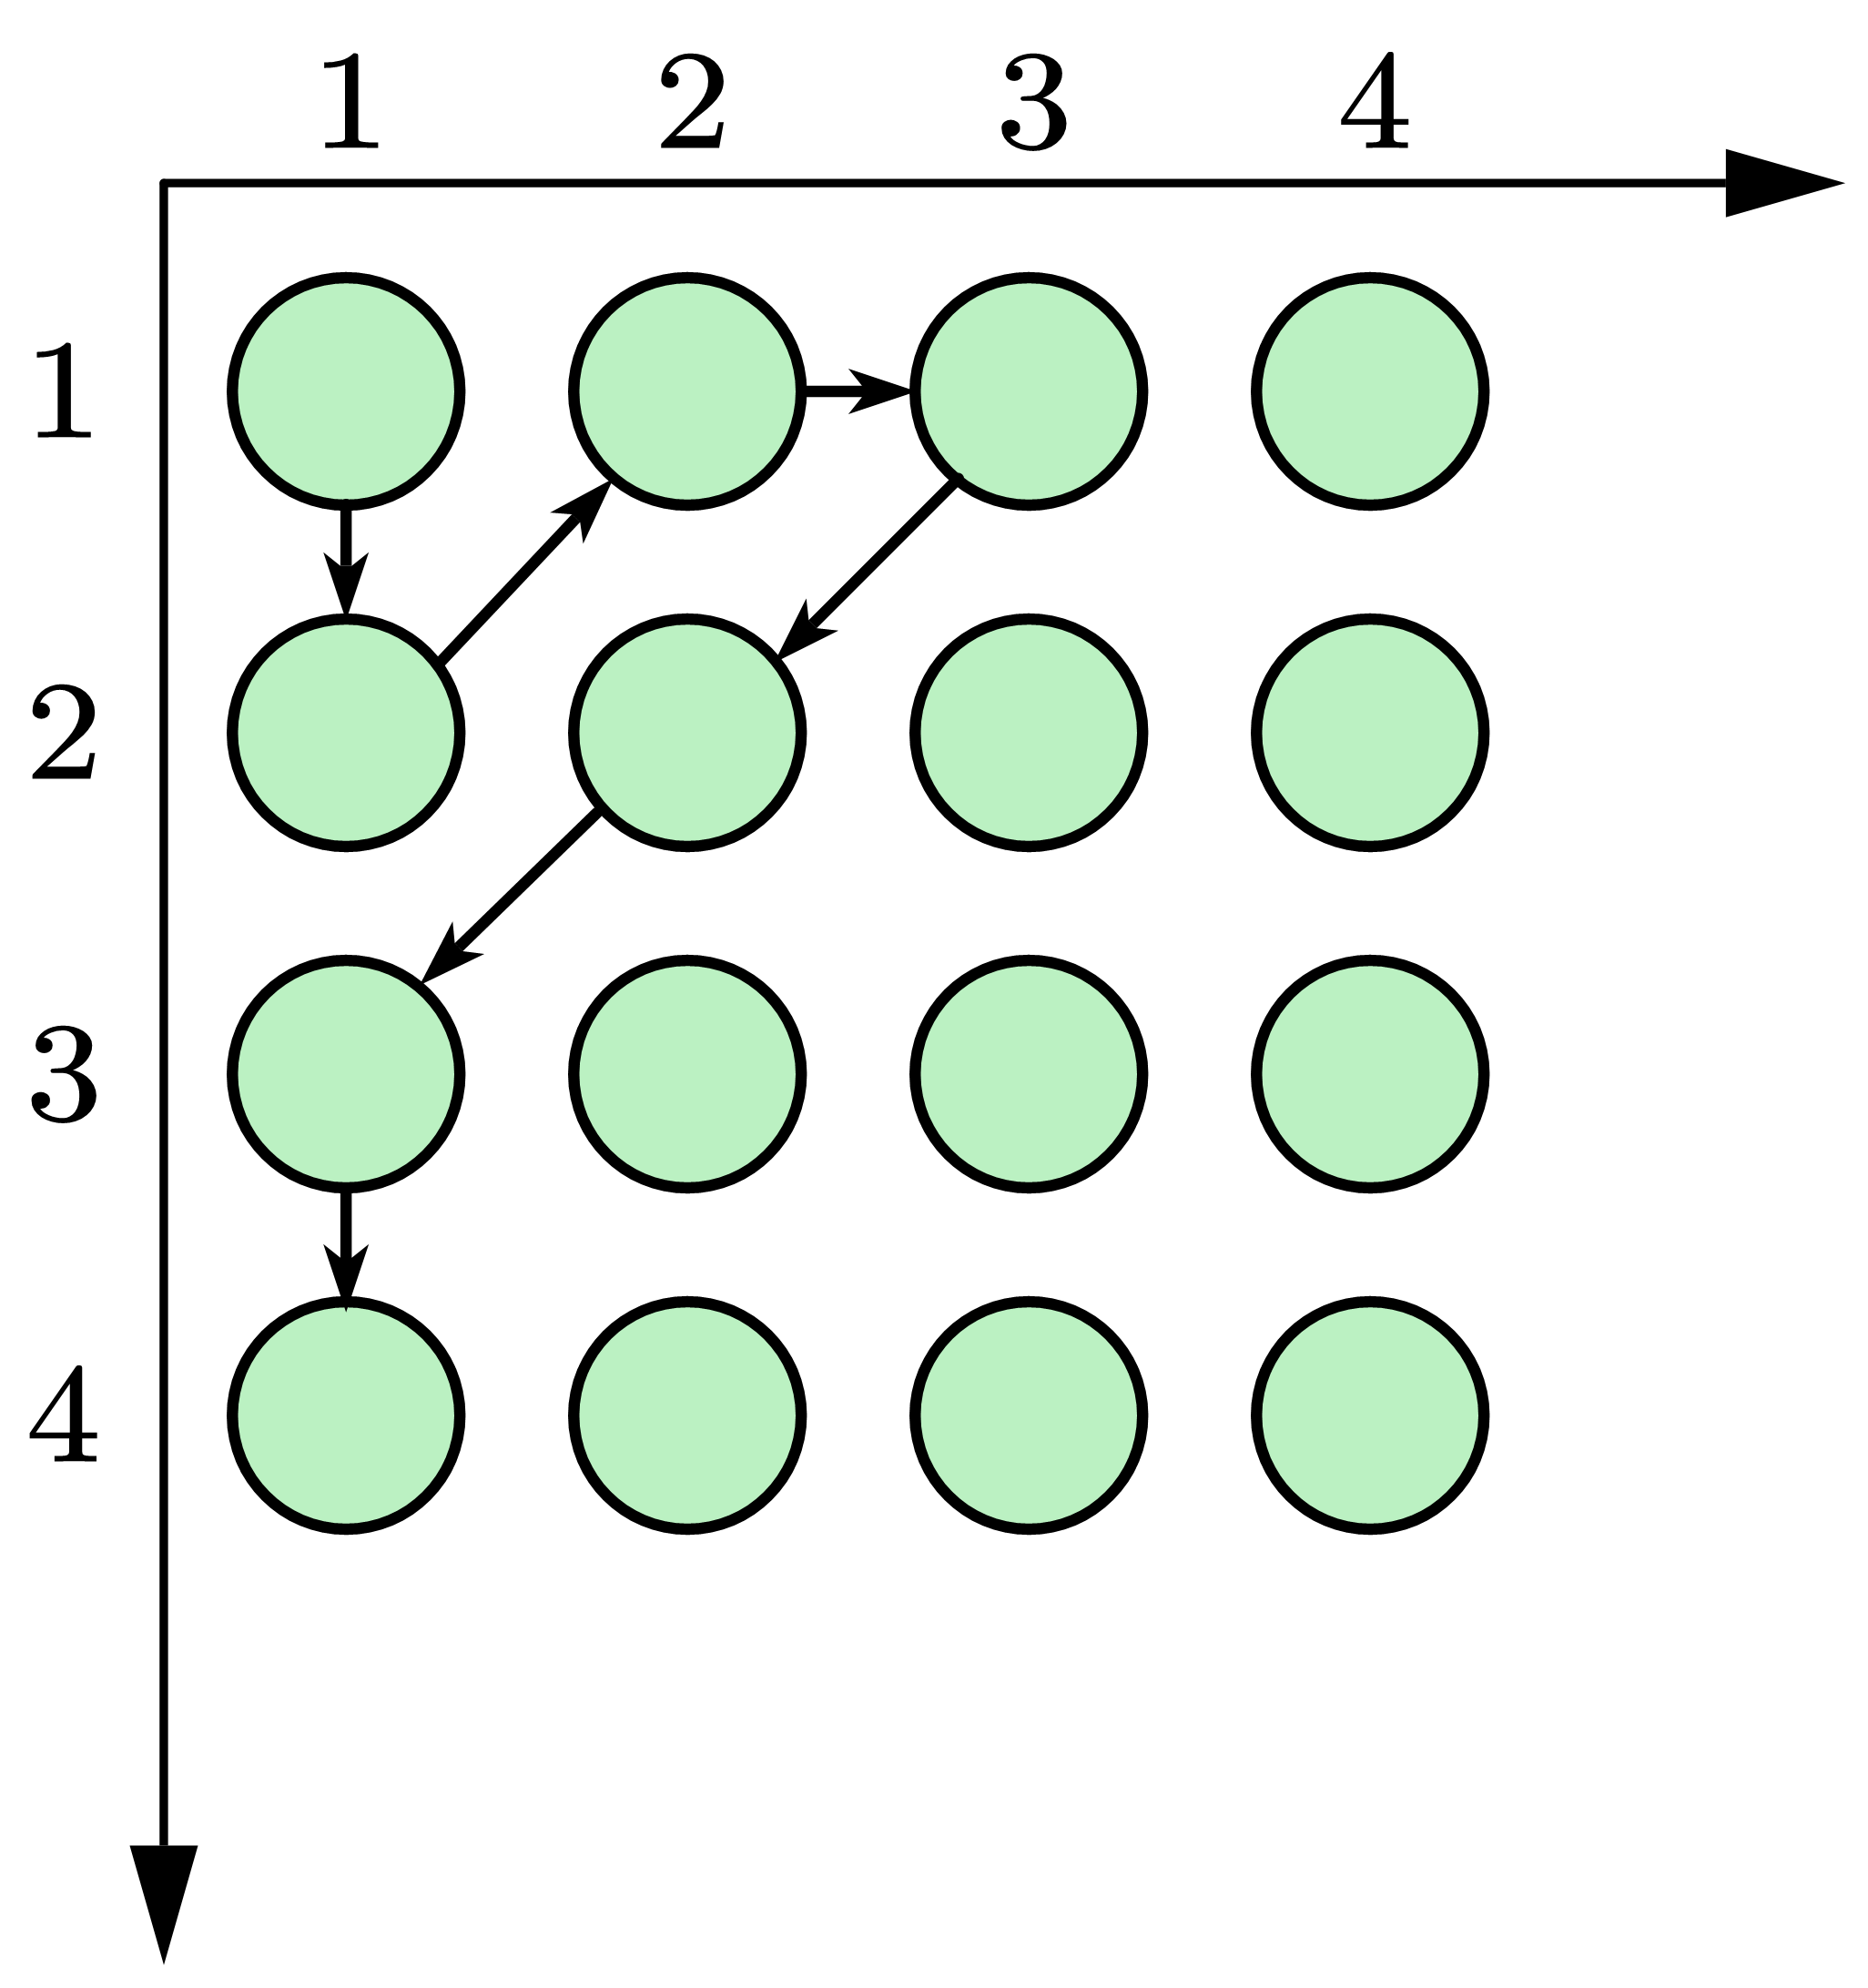
\includegraphics[width=5cm]{figure/2d-list.png}
\end{center}
同时,也有$|\mathbb{R}\times \mathbb{R}|=|\mathbb{R}|$,这是因为对于任意两个实数,可以按10进制展开,然后把它们的数字“交织”在一起形成一个实数。
\item $|\mathbb{R}|=|P(\mathbb{N})|$。$P(X)$为幂集。
\end{enumerate}
\item \emph{连续统假设}:任意实数的不可数子集,与整个实数集等势。这是希尔伯特的23个数学问题的第一个问题。它的另一表述是对基数进行排序:$\aleph_0,\aleph_1,\cdots$,那么$\aleph_{n+1}=2^{\aleph}$,则连续统假设断言:$\aleph_1=2^{\aleph_0}$。也可以说不存在$\aleph$,满足$\aleph_0<\aleph<2^{\aleph}$.

记$P(X)$为无限集合$X$的幂集,前者的基数是$2^{\aleph}$,后者为$\aleph$,\emph{广义连续统假设}认为:如果存在$A\subset P(X)$,且$A$与$P(X)$不等势,那么$|A|\leq |X|$。另一方面,这个假设是说,任意幂集的子集合,其基数不能大于$|X|$,所以广义连续统假设也可以表述为,对于任意无穷基数,不存在严格介于$\aleph$与$2^{\aleph}$之间的基数。哥德尔证明:连续统假设与ZFC是独立的,即假如ZF集合论没有矛盾,则连续统假设不能被ZFC证伪。
\end{enumerate}

仅仅有大小和一组对象还比较简单,给集合中的元素赋予相互关系,就可以构成更复杂的结构.比如给两个元素定义一个距离(距离空间、度量空间),那么就可以定义邻域($U(a)$)、开集、边界($\partial A$)、内部($\text{int} A$或者$\mathring{A}$)、闭包($\overline{A}$).

\subsection{测度}
测度是面积、长度概念的推广,直观上也相当于集合的大小,但基数描述大小主要是从计算的角度出发的,而测度主要是从积分的概念出发。首先要明确的是,测度是一个函数,将一个集合映射为实数,并且这个映射至少满足可加性。这就与范畴\ref{category}、同胚联系起来了。测度映射保持了可加性。以下列出一些比较重要的测度。

与分开密切相关的\emph{豪斯多夫测度(hausdorff)}:

\begin{empheq}{align*}
H^s_{\delta}(A)&=\inf\sbbra{2^{-s}\alpha(s)\sum_{j=1}^{\infty}|C_j|^s\middle| A\subset \bigcup_{j=1}^{\infty}C_j,|C_j|\leq \delta}\\
\alpha(s)&=\frac{\pi^{s/2}}{\Gamma(s/2+1)} \mtag{s维球面积}\\
H^s(A)&=\lim_{\delta\rightarrow 0} H^s_{\delta}(A) \mtag{s维Hausdorff Measure}
\end{empheq}

$|C_j|$为点集的直径,不要把它当成面积,比如对于一个直径为$\delta$的圆,那么$C_j\delta$。在$H^s_{\delta}(A)$的定义中,我们首先对区域进行拆分(为多个球),然后分别计算每个区域的测度,再线性组合起来。又定义\emph{豪斯多夫维数}为:
$$\dim_H(A)=\inf \sbbra{0\leq s<\infty \mid H^s(A)=C\neq 0<\infty}$$

由于计算维数时,仅仅要求测试为有限值,因此$\alpha(s)$和$\frac{1}{2^s}$的系数可以不要。这个维数的特点是,如果$s<\dim_H(A)$,那么有$H^s(A)=0$。$s$大于时,为无穷大。

豪斯多夫维数之所以与分形联系紧密,是因为它很好地描述了“倍增”。考虑二维边长为1的矩形,按边长$\delta$划分为小矩形,每个用圆来代替。那么忽略系数后,$h^s_{\delta}(A)=n^2|C_j|^s=\frac{1}{\delta^2}\delta^s$,要使这个值有限,显然$s=2$。另一个角度来看,一个正方形可以划分为4个小正方形,相当于说如果每条边缩小2倍,那么面积缩小4倍,即维数:
$$s=\frac{\ln 4}{\ln 2}=2$$

\paragraph*{零测集}零测集就是测度为0的集合,直到了十分关键的作用。

\begin{definition}[零测集]
对于集合$A\in\mathbb{R}^n$,如果$\forall \varepsilon>0,$,可以用可数个$n$维立方体覆盖$A$,且这些立方体的体积之和小于$\varepsilon$。则称$A$为零测集。形式化表述为:

$\forall \varepsilon>0,\exists U_n\in(a_n, b_n)^n$,满足$A\subset \cup U_n, \sum |U_n|<\varepsilon$。
\end{definition}

一个典型的例子是有理数集合,它是零测集。因为它是可列的:$\mathbb{Q}={q_1,q_2,\cdots}$,那么取覆盖$U_n=(q_n-3^{-n}\varepsilon,q_n+3^{-n}\varepsilon)$,这个覆盖的测度小于$\varepsilon$。

从以上例子也可以看出,可列集都是零测集。不过零测集不一定可列。
\subsection{邻域($U(a)$)}邻域是包含这个点的集合,并且稍微”抖动“一下也不会离开这个集合.常见的邻域如:

\begin{enumerate}
	\item 开球$U(x,\delta)$.
	\item 去心开球$U_0(x,\delta)$.
\end{enumerate}

\subsection{边界($\partial A$)}几种定义:

\begin{enumerate}
\item 边界=闭包-内部:
	$$\partial A=\overline{A}-\mathring{A}$$
\item 边界=闭包$\cap$补集的闭包:
	$$\partial A=\overline{A}\cap \overline{\Omega-A}$$
\item 边界是一系列点的集合,这些点的每一个领域都至少有一个点属于$A$,也至少有一个点不属于$A$:
	$$\partial A=\{x | \forall U(x), \exists p,q\in U(x), p\in A, q\notin A\}$$
	
	这种定义是最基本的定义.
\end{enumerate}

\subsection{内部($\mathring{A}$)}比较难理解.

\begin{enumerate}
	\item 内部就是非边界点.
	\item 内部是内点的集合,内点是指,存在以这些点为中心的邻域,包含于集合$A$中.
\end{enumerate}

单独一个圆${(x,y)|x^2+y^2=1}$是没有内部的,任取一个点,它的任意领域必然有点不属于这个圆.

假如一个集合内部为空,即$\mathring{A} \neq \emptyset$,相当于只有边界集.以二维平面来看,边界是线,我们在线上找不出一个圆形区域.因此内部为空,即$\nexists \text{非空开子集} O\in A$.反面就是,假如内部非空,则可以找到一个开子集$O$,它满足$O\in A, O\notin X-A$,或者说$\exists O\in X, O\cap X-A=\emptyset$.如下图所示.

\begin{center}
	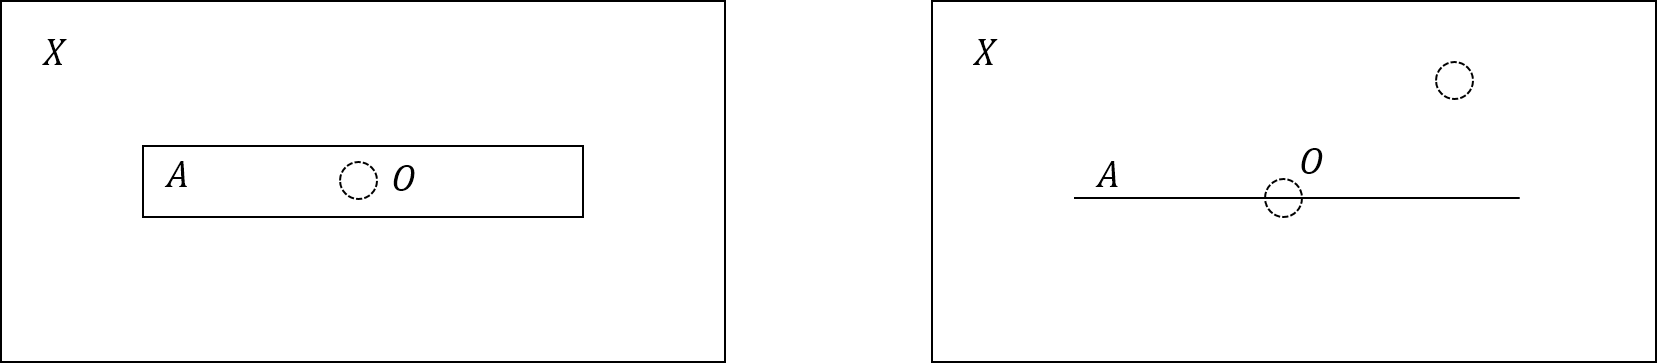
\includegraphics[width=\linewidth]{figure/集合内部非空.png}
\end{center}

再取反面,就可以得到

$$\mathring{A}=\emptyset \iff \forall \text{ 非空开子集 } O \in X, O\cap X-A\neq \emptyset $$

对应上图右边,无论怎么取开集,它都与补集有交.

后面证明Baire定理\ref{thm:baire:proof}时将要用到这种描述.

\subsection{闭包($\overline{A}$)}
在点集拓扑中,集合的闭包是指集合本身与集合的极限点构成的集合.比如一个圆,去掉内部一个点$x_0$,在集合中可以取一系列点,这些点逼近于$x_0$,则$x_0$属于闭包.一个开球的闭包还需要加上恰好在闭球的边界点.

给集合装备一种运算(实际上就是代数结构),假如集合中的元素在这种运算下生成的元素属于集合本身,那么说这个集合满足闭包性质.假如集合不闭合,那么包含这个集合的最小集合就是闭包.

对比这两种定义,可以看出它们本来是一回事,假如把点集拓扑中的“极限”当作一种运算,就是第二种定义.

\subsection{开集与闭集}
非常核心的概念.首先定义开集,闭集自然是对应的,或者取开集的补集.

\begin{enumerate}
	\item 距离空间中,所有点都是内点的集合是开集.
	\item 拓扑学中,所有开集构成拓扑,那么开集就是拓扑的元素.
\end{enumerate}

\subsection{紧性}
一开始有种直观理解是在任意两个点之间,都存在第三个点位于它们之间,假如这两个点恰好取在边界上,则不一定成立。比如平面上有一个洞,在这个洞的边界上取两个点,则它们的连线是在集合外。

现代数学中定义的紧性是基于有限子覆盖:如果一个拓扑空间$X$的所有开覆盖都有有限子覆盖。所谓“开覆盖”是指用开集族覆盖$X$,“子覆盖”就是开集族的子集覆盖$X$。

度量空间中的紧性是指:
\begin{enumerate}
\item 任意序列有收敛子序列,且子序列的极限点属于该集合。
\item 完备且完全有界。
\end{enumerate}

\subsection{稠密}
紧性是集合自身的性质,而稠密性还要涉及集合所处的空间。
\begin{definition}[稠密性]{}
给定拓扑空间$X$与一个子集$A$,如果对于$X$中任意一点$x$,它的邻域与$A$的交集非空。称$A$在$X$中稠密。等价于:

\begin{enumerate}
\item $\bar{A}=X$。
\end{enumerate}
\end{definition}

稠密性的直观理解是全空间中的任意一点都可以由子集中的点逼近。因此在逼近理论中非常有用。

一个简单的例子就是有理数在实数集的稠密性。因此任何一个实数都可以用有理数来逼近。但显然,有理数集自身不是紧的,因为一个有限数列的极限可以是无理数。

\subsection{可分性}
\begin{definition}[可分性]{}
一个距离空间如果有可数个稠密子集,则称为该空间可分。
\end{definition}

\section{集合的运算}
集合的差集$A-B$表示仅在$A$中,而不在$B$中的元素.

用$\Delta$表示对称差,$A\Delta B$表示属于并集,但不属于交集的元素,即仅在$A$或者仅在$B$中的元素.

$$A\Delta B=(A-B)\cup (B-A)$$

\paragraph*{分配律}

\begin{empheq}{align}
(A\cap B)\cup C&=(A\cup C)\cap (B\cup C) \\
(A\cup B)\cap C&=(A\cap C)\cup (B\cap C) \\
(A- B)\cap C&=(A\cap C)- (B\cap C)\\
(A- B)\cup C&=(A\cup C)- (B\cup C)\\
A-\cup B_k &=\cup(A-B_k)\\
A-\cap B_k &=\cap(A-B_k)
\end{empheq}

\paragraph*{de' morgan律}

\begin{empheq}{align}
	\overline{A\cup B}&=\overline{A}\cap \overline{B} \\
	\overline{A\cap B}&=\overline{A}\cup \overline{B} 
\end{empheq}

\section{集合论公理}
\subsection{六大基本公理}

\subsection{选择公理与Zorn引理}
两个定理是等价的,但Zorn引理方便使用一些.

\begin{definition}{选择公理}{sel}
设$(A_i)_{i\in I}$为某集合的一族子集,如果$I\neq \emptyset$,且$\forall i\in I,A_i\neq \emptyset$,则$\prod_{i\in I}A_i\neq\emptyset$.

乘积$\prod_{i\in I}A_i$(选择函数)是映射$f\colon I\rightarrow X$的集合,对$\forall i\in I,f(i)\in A_i$.

另一种表述:$X$非空,且每个元素非空,则存在选择函数.

这种描述中,$X$相当于$(A_i)_{i\in I}$.

\end{definition}

选择函数对每个$i$选择一个元素$f(i)\in A_i$.大致上相当于集合的外积、笛卡尔积.每个选择函数的定义域是相同的,而值域相当于笛卡尔集合中的一个元素.

注意选择公理本身并不是定理,而是人为加入的,仅由前六条公理无法得到选择公理的存在.

\begin{definition}{Zorn引理}{zorn}
设$X$为非空半序集,它的每个全序子集在$X$中均有上界,则$X$至少有一个极大元.
\end{definition}


\chapter{一阶谓词逻辑}
\chapter{形式化系统}

\section{EBNF}
EBNF(Extended Backus–Naur form)可以用来描述上下文无关语法。
\subsection{语法元素}
一个语法需要两类元素,第一是terminal,即最小的元素,第二是规则,描述了元素间的转换关系。定义terminal与规则可以使用以下一些基本操作:
\begin{longtable}{cc}
	\toprule
	含义&	符号\\
	\midrule
	definition	&$=$\\
	concatenation&	$,$\\
	termination	&$;$\\
	alternation	&$|$\\
	optional	&$[\ \cdots\ ]$\\
	repetition	&$\{\ \cdots\ \}$\\
	grouping &	$(\ \cdots\ )$\\
	terminal string	&$"\ \cdots\ "$\\
	terminal string	&$'\ \cdots\ '$\\
	comment	&$(*\ \cdots\ *)$\\
	special sequence	&$?\ \cdots\ ?$\\
	exception&	$-$\\
	\bottomrule
\end{longtable}

\subsection{案例}

\section{CCS}

\subsection{基本技巧}
\begin{enumerate}
  \item 描述一个单元需要多种输入才能进入下一个状态.由于原版的CCS的交互只涉及2个个体,没有3个个体同时交互,那么就需要引入多个状态.比如需要2种资源,就用4个状态:空、等待资源1、等待资源2、准备完成.空状态得到资源1就进入等待资源2,再得到资源2则准备完成.

      但有时如果很明确就是三个个体交互,那么应该也可以让一个个体接受多个输入,其它个体输出,一次完成多个个体交互.
  \item
\end{enumerate} 


\chapter{数论}
\section{基本概念}
\subsection{素数}

\subsection{模运算}
有人认为加、减、乘、除、模是五种最基本的运算,用它们可以表示其它的运算,同时,只有定义了这5种运算,才是完备的。模运算通常用在离散数学中,所以一般的科学技术用的并不多。它可以用来表示周期性。
\subsubsection{同余关系}
同余关系是指
$$a\equiv b \pmod n$$
利用模$n$同余关系可以将整数划分为$n$等价类,这些等价类构成模$n$的完全剩余系,记为
$$\mathbb{Z}_n=\{0,1,\cdots,n-1\}$$

从完全剩余系中去掉与$n$不互素($\gcd(n,k)=1$)的那些数(显然0不是不互素的,$\gcd(n,0)\neq 1$),剩下的叫简化剩余系,比如
$$Z_9^\star=\{1,2,4,5,7,8\}$$
注意$3,6$与9是不互素的。
\subsubsection{模运算的性质}
\paragraph*{四则运算}以同余关系定义的运算法则有以下一些。

如果$a\equiv b\pmod n$,那么有
\begin{empheq}{align*}
a+k\equiv b+k&\pmod n\\
a^k\equiv b^k&\pmod n
\end{empheq}

以同余关系定义,有点类似于对方程两边进行操作,从一个预定义的关系出发。也可以以直接代数运算来定义,此时是从一边进行推导到另一边。

\begin{empheq}{align*}
(a\bmod n+b\bmod n)\bmod n&=(a+b)\bmod n\\
(a\bmod n\times b\bmod n)\bmod n&=(a\times b)\bmod n
\end{empheq}

\paragraph*{乘法逆}假设$gcd(n,k)=1$,那么存在$k^{-1}$,有$k\times k^{-1}\equiv 1  \pmod n$。这里是对互素的情况,如果不互素,一般好像定义乘法逆为0。

\paragraph*{重复序列}使用模运算$x \mod n$可以生成$0,1,\cdots,n-1,0,1,\cdots,n-1,\cdots$的重复序列。使用$((x-1)\mod n) +1$可以生成$1,\cdots,n,1,\cdots,n,\cdots$的重复序列,在数组循环的时候很有用。
\subsection{Euler定理}
定义欧拉函数$\varphi(n)$,其含义是不超过$n$且与$n$互素的元素个数,也相当于简化剩余系的个数。
\begin{empheq}{align*}
\varphi(1)&=1\\
\varphi(p)&=p-1,\ p\text{为素数}\\
\varphi(p^k)&=p^{k-1}(p-1)=p^k-p^{k-1}=p^k\left(1-\inv{p}\right),\ \text{如果}p\text{为素数}\\
\varphi(n_1n_2)&=\varphi(n_1)\varphi(n_2),\ \text{如果}\gcd(n_1,n_2)=1\\
\varphi(n)&=n\prod_{i=1}^{n}\left(1-\inv{p_i}\right),\ \text{如果}n=\prod_{i=1}^{n}p_i^{a_i},p_i\text{为素数}
\end{empheq}
\chapter{组合论}
\section{基本原理}
\subsection{排列数与组合数}
\subsubsection{排列数}
\begin{definition}
从$n$种不物品中不放回取出$k$种物品,再将取出的物品进行排列,则最终可以得到不同的排列为排列数:
$$A(n,k)=\frac{n!}{(n-k)!}$$
\end{definition}

\subsubsection{组合数}
\begin{definition}
从$n\geq 0$种不物品中不放回取出$k$种物品,则不同的取法数量为组合数:
\begin{empheq}{align}
P(n,k)&=\binom{n}{k}=\frac{A(n,k)}{k!}=\frac{n!}{(n-k)!k!}\\
\binom{n}{0}=\binom{n}{n}=1,\quad n\geq 0
\end{empheq}
\end{definition}

\subsection{组合论等式}
\begin{empheq}{align*}
\binom{n}{k}+\binom{n}{k+1}=\binom{n+1}{k+1}
\end{empheq}

\subsection{鸽巢原理}
基本的表述是:将一个空间分成$n$类,那么从这个空间中取出$n+1$个元素,必然至少有两个元素处于同一类中.

使用鸽巢原理最重要的就是如何分类.对于不同的问题分类标准不同,比如对于数空间:正负、有理无理、奇偶等等.

\begin{example}
在二维平面上的整数格点中取5个点,则必然存在另一个整数格点,恰好位于这5个点中某两个点连线构成的线段上.

分类标准就是奇偶性,一个点的两个坐标奇偶性只有4种情况,就可以用鸽巢原理了.如(奇,奇),(奇,奇)的中点就是(偶,偶).
\end{example}

\section{组合论例子}
\subsection{样本问题}
\begin{example}
\textbf{(滑动窗口的采样重叠问题)}考虑滑动窗口,假设长度为$n$,滑动距离为1,那么每两个相邻的窗口,有$n-1$个重叠样本。假设从两个相邻的窗口中,每个窗口中取$m$个样本,问相同样本数量的分布。
\end{example}
\begin{solution}
显然地,全空间为$\binom{n}{m}^2$. $n$个样本可分为$1+(n-1)$个样本。取$m$个样本,分为两种情况:取或者不取前1个样本。则取两组样本时,有4种情况,一个一个列出来然后计算。

首先考虑最基本的情形:全不重叠。

假设第一组取了前1个样本,则第二组假如也取前1个,那么剩下$m-1$个要从$n-1-(m-1)=n-m$个中取。
\begin{empheq}{align*}
&\frac{\underbrace{\binom{n-1}{m-1}}_{\text{1取}}\left(\underbrace{\binom{n-m}{m-1}}_{\text{2取}}+\underbrace{\binom{n-m}{m}}_{\text{2不取}}\right)+\underbrace{\binom{n-1}{m}}_{\text{1不取}}\left(\underbrace{\binom{n-1-m}{m-1}}_{\text{2取}}+\underbrace{\binom{n-1-m}{m}}_{\text{2不取}}\right)}{\binom{n}{m}^2}\\
=&\frac{\underbrace{\binom{n-1}{m-1}}_{\text{1取}}\binom{n-m+1}{m}+\underbrace{\binom{n-1}{m}}_{\text{1不取}}\binom{n-m}{m}}{\binom{n}{m}^2}
\end{empheq}

再考虑有$k,k\leq m$个重叠的。

$k=m$比较显然。第一组只能在$n-1$个中取$m$个:
\begin{empheq}{align*}
\frac{\binom{n-1}{m}}{\binom{n}{m}^2}=\frac{n-m}{n}\bigg/\binom{n}{m}
\end{empheq}

对于其它情形。此时首先第一组任取,然后第二组取的时候先从第一组里面取$k$个,然后从剩下的取$m-k$个。第一组要分情况,假如第一组取了前1个,那么第二组只能从$m-1$个取$k$个,而且剩下的$m-k$个也分取或者不取两种情形,假如取了前1个,那么要从$n-1-(m-1)$个中$m-k-1$个;假如不取,从$n-1-(m-1)$个取$m-k$个。
\begin{empheq}{align*}
&\frac{\underbrace{\binom{n-1}{m-1}}_{\text{1取}}\binom{m-1}{k}\left(\underbrace{\binom{n-m}{m-k-1}}_{\text{2取}}+\underbrace{\binom{n-m}{m-k}}_{\text{2不取}}\right)+\underbrace{\binom{n-1}{m}}_{\text{1不取}}\binom{m}{k}\left(\underbrace{\binom{n-1-m}{m-k-1}}_{\text{2取}}+\underbrace{\binom{n-1-m}{m-k}}_{\text{2不取}}\right)}{\binom{n}{m}^2}\\
=&\frac{\underbrace{\binom{n-1}{m-1}}_{\text{1取}}\binom{m-1}{k}\binom{n-m+1}{m-k}+\underbrace{\binom{n-1}{m}}_{\text{1不取}}\binom{m}{k}\binom{n-m}{m-k}}{\binom{n}{m}^2}
\end{empheq}

以下给出一些算例:
\begin{enumerate}
\item 假设$n=1000,m=50$,则完全不重合的概率$P(0)\simeq 0.07$,前几个概率值如下:
\begin{empheq}{align*}
P(1)&\simeq 0.2\quad &P(2)&\simeq 0.2659\\
P(3)&\simeq 0.2259\quad & P(4)&\simeq 0.1378\\
P(5)&\simeq 0.0644 \quad & P(6) &\simeq 0.0239\\
P(7)&\simeq 0.0072 \quad & P(8) &\simeq 0.001856
\end{empheq}
$$\sum_{k=1}^{7}\simeq 0.86$$

可见,大概率只有少数几个样本会重合。
\end{enumerate}
\end{solution}

\begin{example}
\textbf{(随机采样的覆盖面)}$N$个样本,有放回取$n$个,问这些样本中不同样本个数$k,k\leq \min(N,n)$的分布。

训练模型时,经常是随机采样,通过这个问题,主要是看看需要抽多少次,才能使所有样本都被抽到的概率大于一定值。
\end{example}
\begin{solution}
全空间显然为$N^n$。
\end{solution}
\begin{example}\label{birthday_paradox}
\begin{theorem}[生日悖论]{}
	$N$为正整数,从中独立、随机选择$Q$个元素$x_1,\cdots,x_Q$,则
	$$\frac{Q(Q-1)}{4n}\leq P(\exists (i,j),x_i=x_j)=\frac{n\times(n-1)\times(n-Q+1)}{}\leq \frac{Q^2}{2N}$$
\end{theorem}

在上面的下界中,取$Q=\sqrt{2N}$,那么下界就接近$\fh$了。取1年365天,那么只要取$\sqrt{2\times 364}\approx 27$个人,其中有两个人同月同日生的概率就大于$\fh$。
\end{example}


\chapter{密码学}
\section{基本概念}
\subsection{密码学研究的问题}
\subsubsection{加密解密}
希望某些内容只能被一部分人知道,向其它人隐藏相关信息。是最基本的问题。其它的问题需要基于这个问题。为解决这个问题,需要构建一个系统。

对称密码体制是指双方共享密钥,整个系统由以下元素构成:

\begin{description}
\item[明文空间$P$] 所有可能的明文。
\item[密文空间$P$] 明文加密后得到密文。
\item[密钥$K$] 我们可以传送操作,比如传送加密和解密算法,但这样很困难,不同的机器运行的程序不一定相同。因此需要使用密钥的体制,密钥易于传送。
\item[加密算法$e_K$和解密算法$d_K$] $e_K: P\rightarrow C,\ d_K: C\rightarrow P$,且满足$d_K(e_K(x))=x$,但是需要注意通常$e_K(d_K(x))\neq x$,所以这里是非交换代数。
\end{description}

有对称的就有非对称的,公钥密码体制就属于这一类,除了明文和密文空间以外,现在密钥有2个:
\begin{description}
\item[公钥$SK$] 公开的,所有人都知道。
\item[私钥$PK$] 私有,只有自己知道。给定公钥生成算法和公钥$PK$,不可以得到$SK$。
\item[加密算法$E_{PK}$和解密算法$D_{SK}$] 加密$C=E_{PK}(M)$,解密$M=D_{SK}(C)$。假设想向对方传递消息,只有对方可以知道,就需要用对方的公钥加密,对方用私钥解密。
\end{description}
\subsubsection{身份验证}

\subsubsection{消息摘要}

\subsubsection{判断密码体制的安全性}
密码学中使用的都是有限域,通过穷举,一定是可以得到解的,只是穷举的效率一般很低。还可以通过随机搜索, 一个典型的例子就是“生日悖论”\ref{birthday_paradox}。



\section{加密原理}
\subsection{椭圆曲线}
椭圆曲线是由方程确定的曲线,可以是连续的,或者离散的。
\subsubsection{连续域}
由方程
$$y^2=x^3+ax+b,4a^2+27b^2\neq 0, a,b,x,y\in\mathbb{R}$$
确定的曲线再加上一个无穷远点$O$构成的集合叫椭圆曲线。在曲线上取2不相等的点,连线与曲线自身一般会交于第三个点。

在这个集合上可以定义加法$\oplus$:
\begin{enumerate}
\item $P\oplus O=O\oplus P=P$
\item 对于$P=(x_1,y_1),Q=(x_2,y_2)$:
\begin{enumerate}
	\item 如果$x_1=x_2,y_1=-y_2$,即两点的连续平行于$y$轴,那么$P+Q=O$。直线与曲线只有1个交点。
	\item 如果$P=Q$,则$P\oplus Q=2P=R'$,$R'$是过$P$的切线与曲线的第二个交点对$x$轴的对称点。即直线与曲线只有2个交点。
	\item 如果$x_1\neq x_2$,那么定义$P\oplus Q=R'$,$R'$为$P,Q$的连线与曲线自身的第三个交点,再把这个交点对$x$轴对称,或者对$y$取反。这个定义与上一个是一致的,当两个点趋近时,连线就趋于切线。

\end{enumerate}
	
详细的结果按以下公式给出。假设$y_1\neq 0,x_1\neq x_2$,那么
\begin{empheq}[left=\empheqlbrace]{align*}
	x_3&=-x_1-x_2+k^2\\
	y_3&=-y_1+k(x_1-x_3)
\end{empheq}
其中$k$是斜率:
\begin{empheq}[left={k=\empheqlbrace}]{align*}
	\frac{y_2-y_1}{x_2-x_1}&\\
	\frac{3x_1^2+a}{2y_1}&,\text{ if }P=Q
\end{empheq}

这个公式对于$P=Q,P\neq Q$都可以用。
\end{enumerate}
配上加法后,椭圆曲线构成了交换群,无穷远点是单位元。

\subsubsection{离散域}
观察到在连续域中进行计算,需要三种基本运算:加法、减法、乘法、乘法逆运算、取反。这些运算可以定义在$\mathbb{Z}_n$上。此时记椭圆曲线为$E_n(a,b)$,五种基本运算是对应的运算再$\mod n$。乘法逆运算是指$xy\equiv 1 (\mod 23)$。

给出一个实际的例子。取$E_{23}(1,1),P=(3,10),Q=(9,7)$。
\begin{enumerate}
\item 计算$-P$。结果是$(3,-10) \mod 23=(3, 13)$。
\item 计算$P+Q$。斜率是$-\fh=(-1)\times \fh=\left((-1 \mod 23) \times (2^{-1}) \right)\mod 23=11$。注意$2^{-1}=12$,因为$2\times 12 \mod 23=1$。由于$\left((a\mod n)\times b\right)\mod n=(a\times b)\mod n$,所以之前也可以用$(-1\times 12)\mod 23=11$。

现在可以按之前的公式进行计算。$x_3=-x_1-x_2+k^2=(-3-9+11^2)\mod 23=17$,$y_3=(-10+11\times (3-17))\mod 23=20$。所以$P\oplus Q=(17,20)$。
\item 计算$2P$。斜率$k=\frac{3\times 9+1}{2\times 10}=\frac{1}{4}=1\times 4^{-1}=6$。那么$x=-3-3+62=30\equiv 7(\mod 23)$,$y=-10+6\times(3-7)=12$,因此$2P=(7,12)$。
\end{enumerate}

\section{经典密码体制}
\subsection{RSA}
\subsubsection{执行过程}
\begin{enumerate}
\item 选择大素数$p,q$,通常需要512位,需要使用素数筛法来生成。
\item 计算$n=pq, \varphi(n)=(p-1)(q-1)$。
\item 选择整数$e$,满足$1\leq e\leq \varphi(n),\gcd(\varphi(n),e)=1$。
\item 计算$d\equiv e^{-1}\pmod{n}$。
\item 公开$n,e$,$e$是公钥;私有$p,q,d$,$d$是私钥。
\end{enumerate}


%\chapter{计算理论}

\section{理解计算}
\subsection{计算的一般模式}
下图展示了计算的一般模式:

\begin{center}
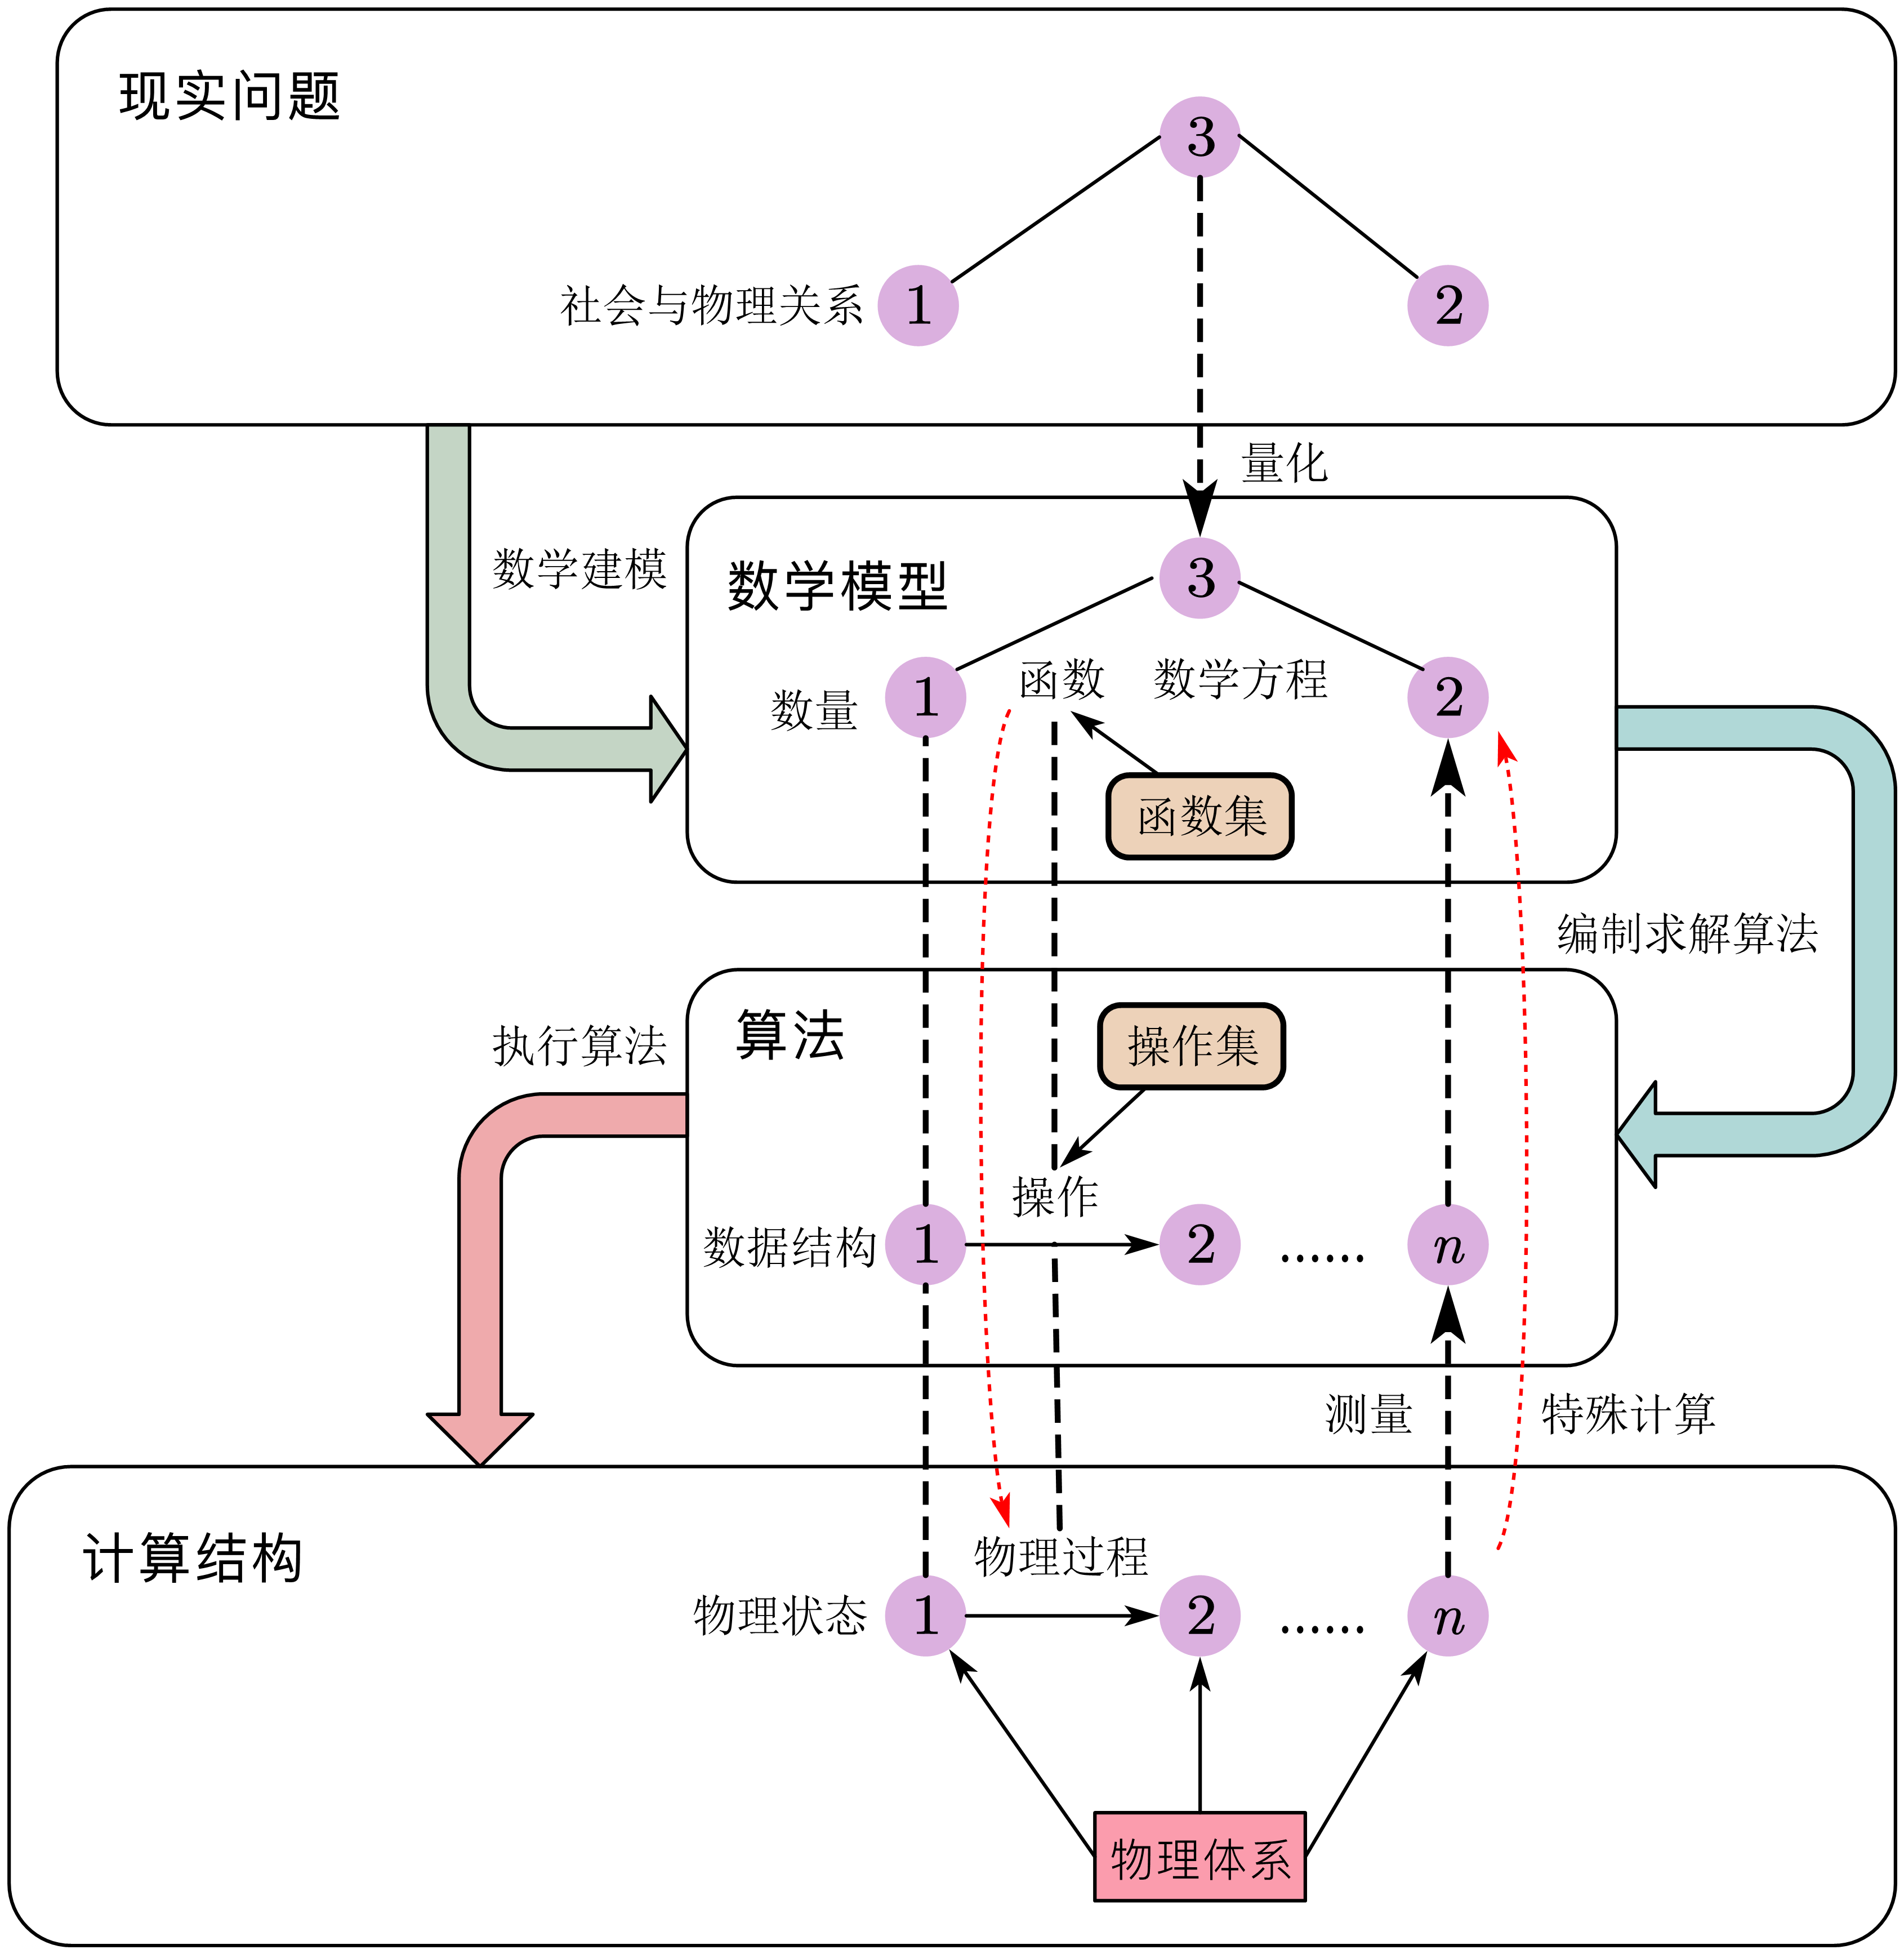
\includegraphics[width=14cm]{figure/General Computing.png}
\end{center}

图中画红线的是特殊计算,比如光子计算、蛋白质计算、神经计算等等,以区别于传统的诸如使用计算机编程的计算。


\section{量子计算}


\part{几何学}
\chapter{平面几何}


\section{运动与曲线}
\subsection{圆沿着曲线滚动}
\subsubsection{沿直线滚动}
\paragraph*{摆线}圆沿着一条直线滚动,其边上一点形成的曲线叫摆线。
假设初始时圆心坐标为$(0,r)$,初始的圆上的点为$(0,0)$。从几何角度推导如下图:

\begin{center}
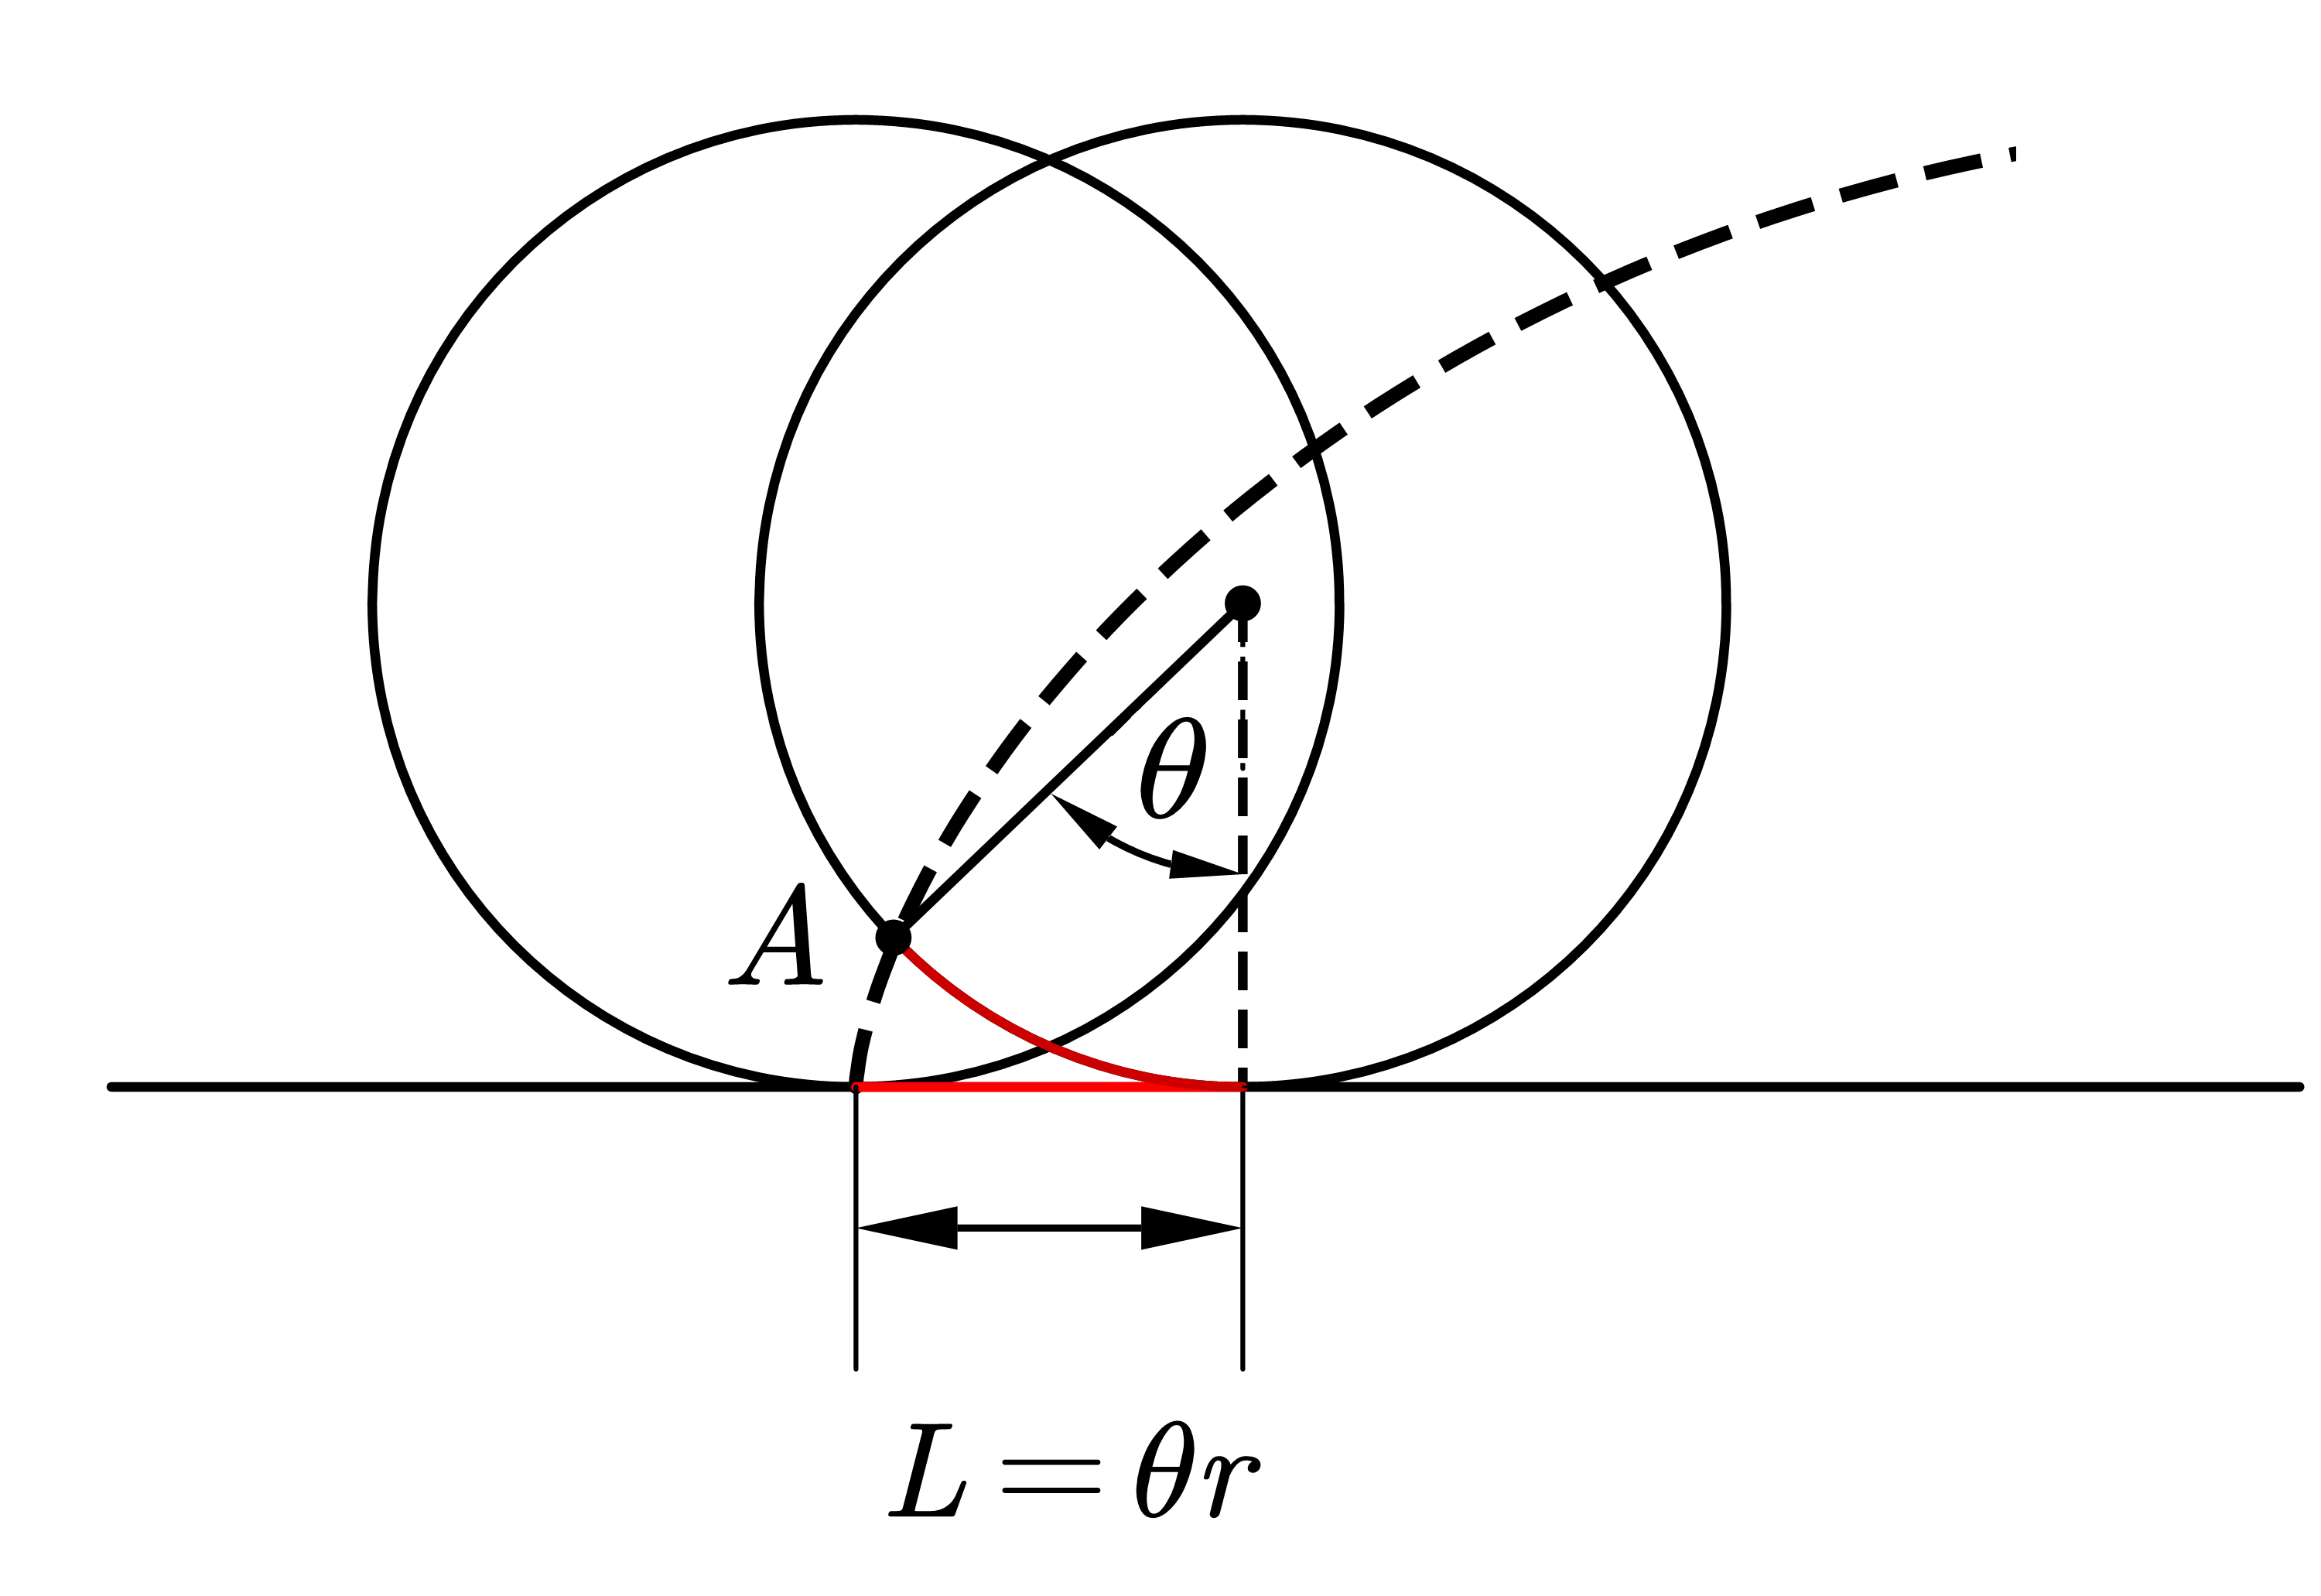
\includegraphics[width=8cm]{figure/摆线.png}
\end{center}

图中两段红线的长度应该是相等的。求$A$点的坐标时可以先把圆心平移到圆点,此时坐标为
\begin{empheq}{align*}
x&=r\cos\sbra{-\frac{\pi}{2}-\theta}\\
y&=r\sin\sbra{-\frac{\pi}{2}-\theta}
\end{empheq}
再平移回去,$x$坐标增加$L=r\theta$,$y$坐标增加$r$。即有:
\begin{empheq}{align*}
	x&=r\sbra{\theta-\sin\theta}\\
	y&=r\sbra{1-\cos\theta}
\end{empheq}

从另一个角度来看,假如沿直线滚动了长度$L$,那么我们需要在圆上找一点,使得其弧长恰好也是$L$。

\subsubsection{沿圆滚动}
如下图所示,小圆沿着大圆滚动:

\begin{center}
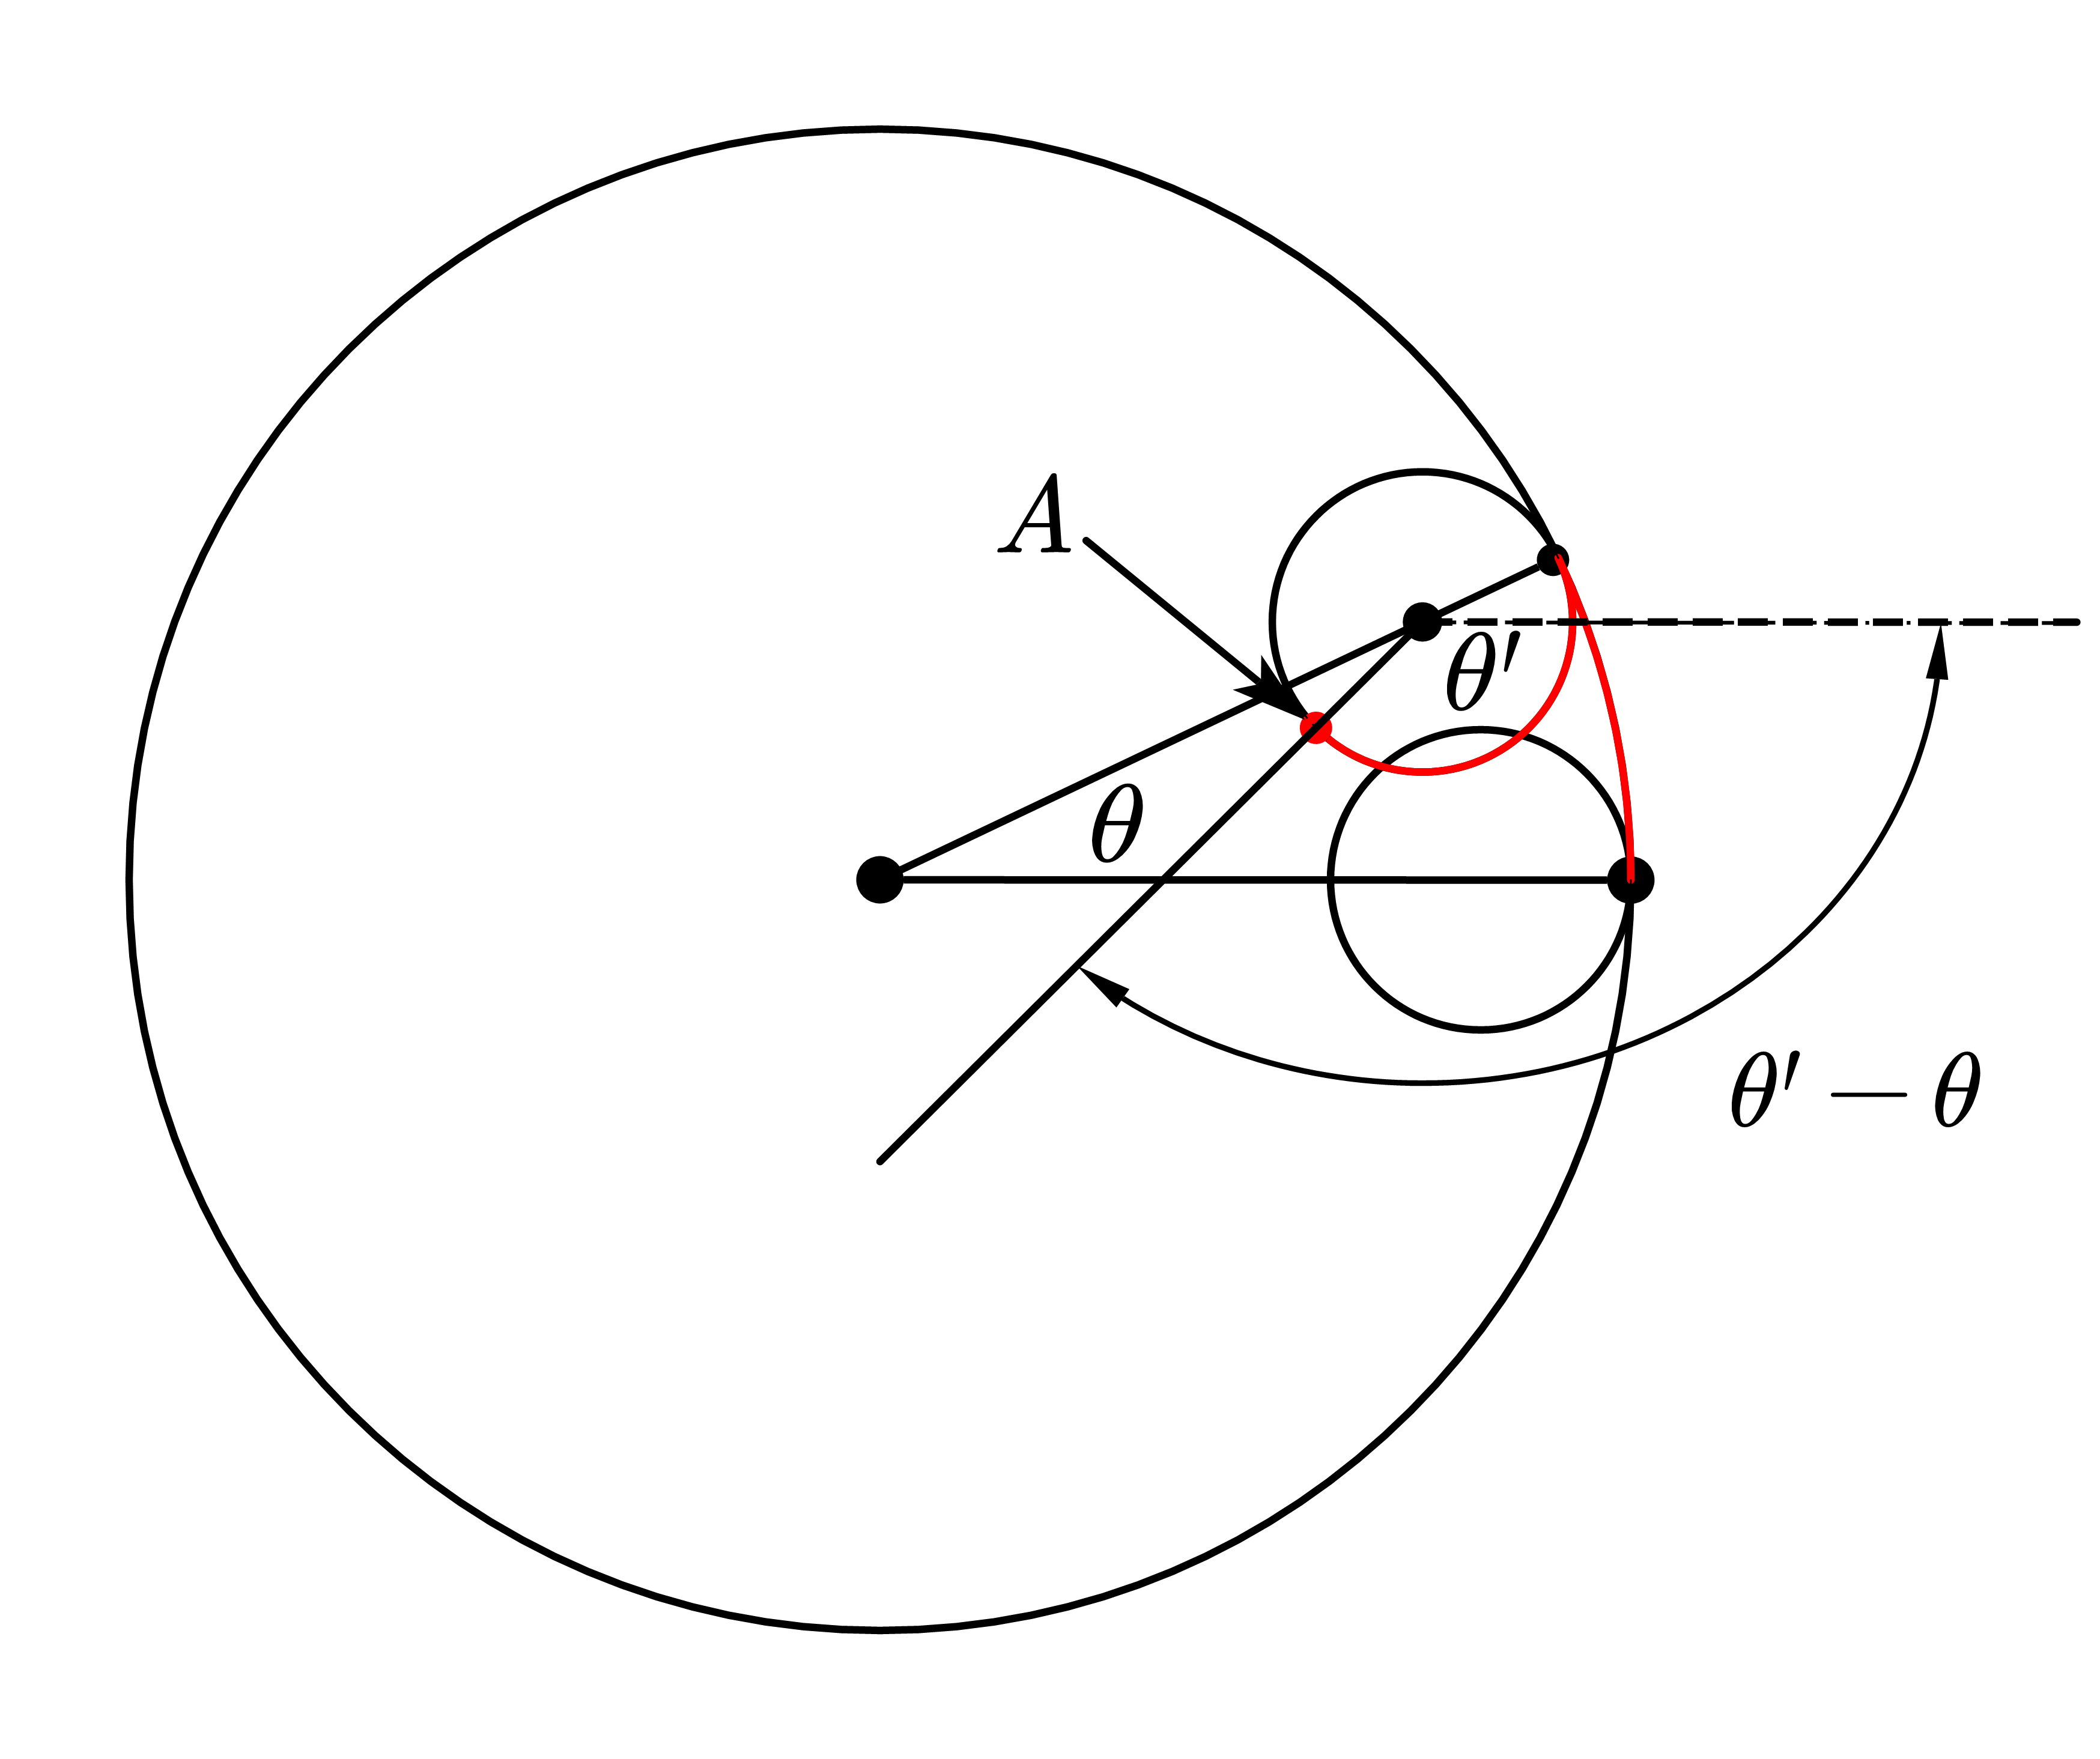
\includegraphics[width=8cm]{摆线(圆上).png}
\end{center}

计算时可以没用找弧长为$L$的方法。


\chapter{空间几何}
%\chapter{投影}
\section{几何体}
\subsection{$n$维球}\label{ndsphere}
对于$n$维球,设半径为$R$,那么体积
$$V_n=\frac{\pi^{n/2}}{\Gamma(n/2+1)}R^n$$
$n-1$维球表面积为
$$S_{n-1}=\frac{\dif V_n}{\dif R}=\frac{2\pi^{n/2}}{\Gamma(n/2)}R^{n-1}$$
这里求表面积非常巧妙,将半径无穷小增加,则体积也增加,增加的比例于表面积有关。因此直接求导。

假如取单位球$R=1$,那么可以看出,当维数$n$增加时,体积趋向于0。这可能有点反直觉,因为高维球应该是“包含”低维球的,比如对于任意一个低维球中的点,只要把其它维度设成0,就可以变成高维球的点,为什么高维球的体积反而小了呢?

这主要是由于低维体在高维中,体积是0。比如二维平面在三维空间中,体积就是0。
\chapter{计算几何}
\section{几何数据结构}

\subsection{四叉树}

\section{几何操作}
\subsection{基本操作}
\subsubsection{旋转}
\paragraph*{2D旋转矩阵}
\begin{empheq}{align*}
R_x(\theta)&=\begin{bmatrix}
	\cos \theta &-\sin\theta\\
	\sin\theta& \cos\theta
\end{bmatrix}\\
x'&=R_x(\theta)x=\begin{bmatrix}
x_1\cos\theta-x_2\sin\theta\\
x_1\sin\theta+x_2\cos\theta
\end{bmatrix}
\end{empheq}

此处的$\theta$是与$x$轴形成的角度。
\paragraph*{3D旋转矩阵}

\begin{empheq}{align*}
R_x(\theta)&=\begin{bmatrix}
	 1& 0 &0\\
	0 & \cos \theta &-\sin\theta\\
	0& \sin\theta& \cos\theta
\end{bmatrix}\\
R_y(\theta)&=\begin{bmatrix}
	\cos \theta& 0 &\sin\theta\\
	0 & 1 &0\\
	-\sin\theta& 0&\cos\theta
\end{bmatrix}\\
R_z(\theta)&=\begin{bmatrix}
	\cos\theta& -\sin\theta &0\\
	\sin\theta & \cos \theta &0\\
	0& 0& 1
\end{bmatrix}
\end{empheq}

\paragraph*{旋转对齐}考虑向量$\bm{a},\bm{b}$,希望旋转$\bm{a}$使之与$\bm{b}$对齐,即求旋转矩阵$R\bm{a}=\bm{b}$。

公式是
$$R=I+\bm{v}_{\times}+\frac{1-c}{s^2}\bm{v}_{\times}^2$$

其中$\bm{v}=\bm{a}\times \bm{b}, s=\|\bm{v}\|,c=\bm{a}\cdot\bm{b}$,
$$\bm{v}_{\times}=\begin{bmatrix}
0 & -v_3 & v_2 \\
v_3 &0 & -v_1\\
 -v_2& v_1& 0
\end{bmatrix}$$
叫skew-symmetric cross-product matrix。
\subsubsection{}
\chapter{射影几何}

\chapter{光学}
\section{折射}

\chapter{计算机图形学}
%\input{图形计算}
\section{颜色}

\section{光线追踪}
\subsection{路径追踪基本}
要利用路径跟踪算法,实现一个全局光照模型,至少需要解决四方面的问题:
\begin{enumerate}
\item 场景、物体、材料的数据结构,物体数据结构中需要存储坐标和一些必要的属性缓存信息,如法向量。材料的数据结构中主要存储材料的参数。
\item 实现光线与场景的交互,包括计算交点、折射、反射、漫反射。
\item 实现颜色模型,即处理颜色如何叠加。
\item 输出可视化结果。
\end{enumerate}

对于第一个问题,本文使用三角面片来表示物体,每个物体用一个基类表示,所有物体继承这个基类,内部存储三角面片的坐标、面法向量、顶点法向量。由于是光线追踪类模型是从屏幕的像素点发射光线到场景中,因此主要问题是把屏幕“放置”到世界中,确实3D坐标。不必考虑怎么将3D坐标投影到屏幕的2D坐标。

本文采用的方式是将屏幕放在XY平面,屏幕中心就是原点。如下图所示:

\begin{center}
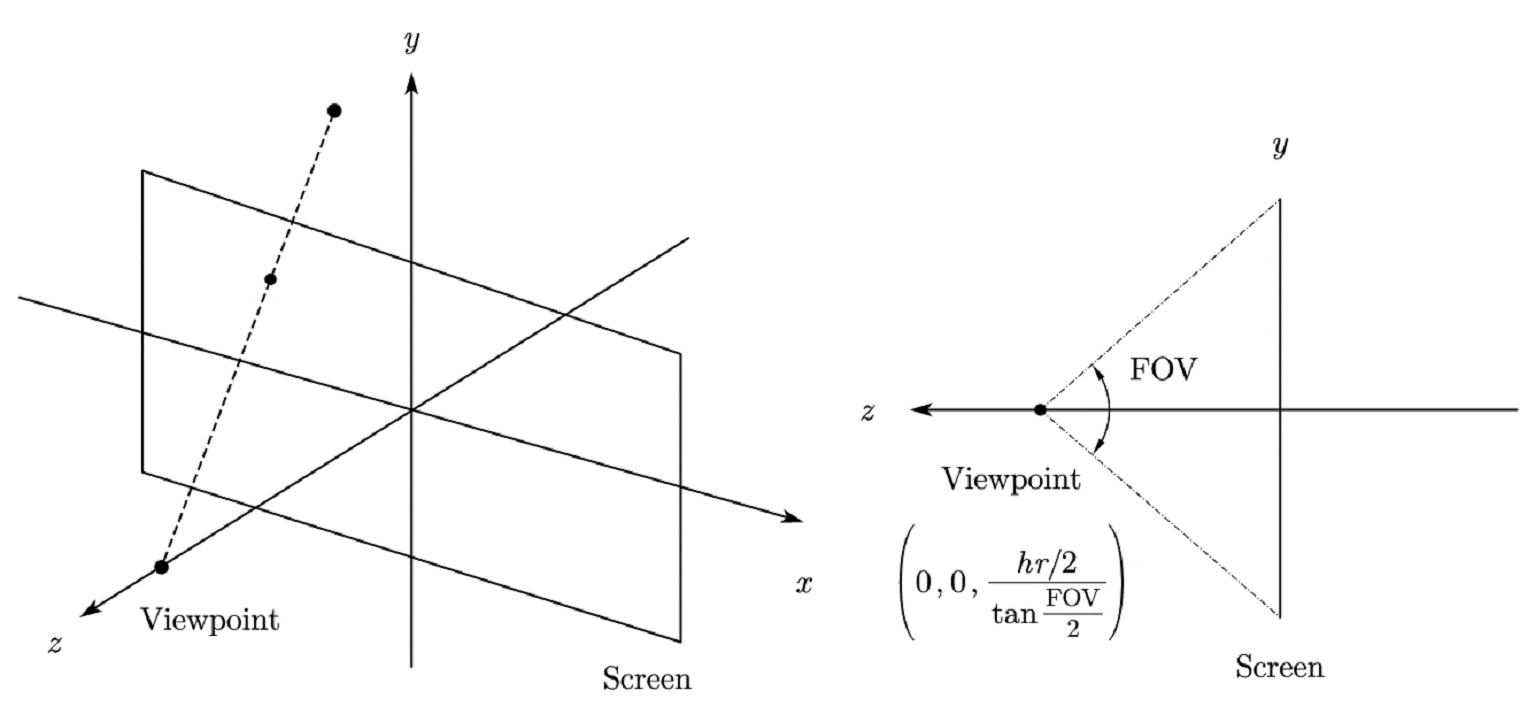
\includegraphics[width=10cm]{figure/screen.png}
\end{center}

对于第二个问题。路径追踪的思路是从每个像素点射出若干条射线,射线如果遇到三角面片,会以一定概率发生反射、折射、漫反射,这由材料的属性决定,最终假如遇到了光源,就可以计算像素的颜色了。示意图如下:

\begin{center}
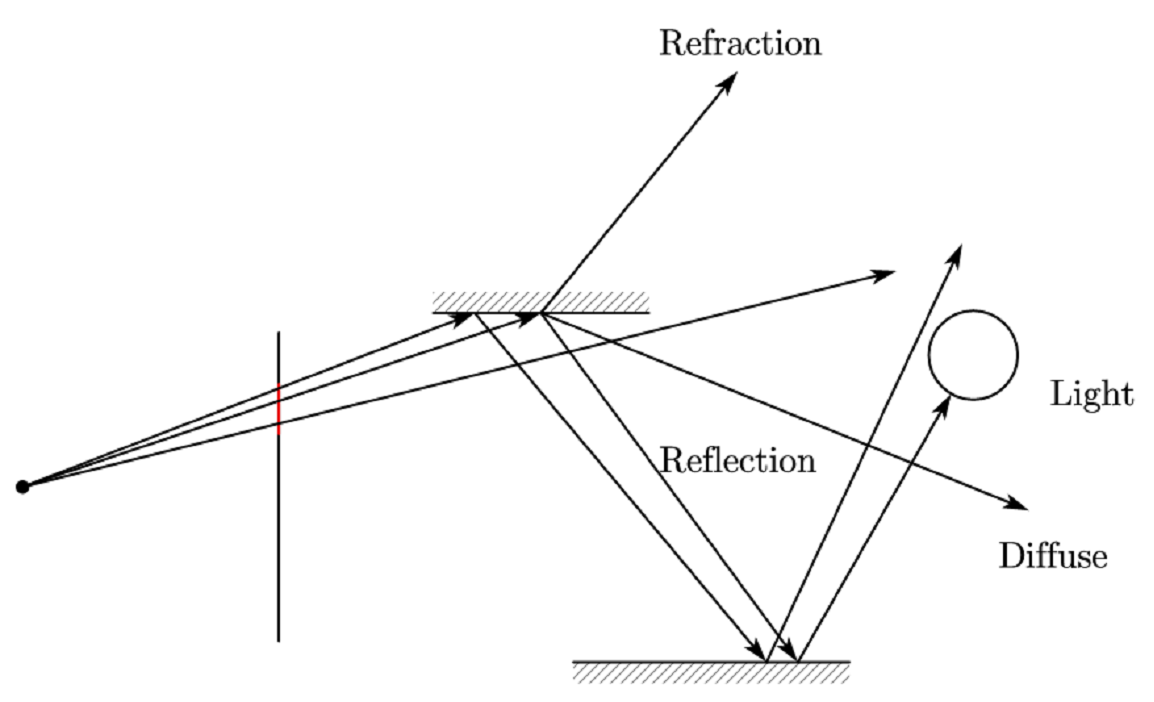
\includegraphics[width=10cm]{figure/path tracing.png}
\end{center}

一个首要的问题就是计算射线与三角面片的交点。本文使用了NanoRT库,它就是用来计算交点。使用这个库是因为它使用了加速算法,如果自己实现一遍,手动遍历所有面片来计算交点,则效率会很低。

在计算交点以后,需要计算折射、反射与漫反射的概率。按下式给出:

\begin{center}
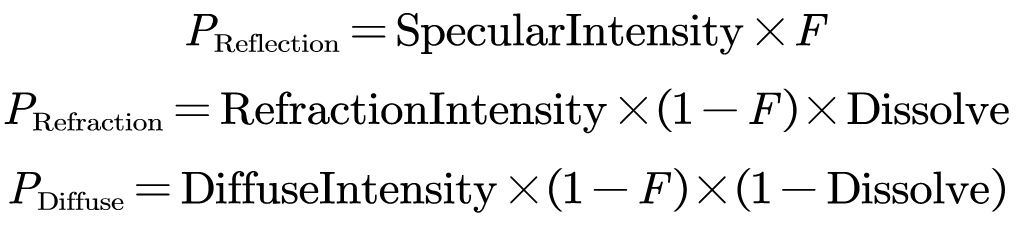
\includegraphics[width=6cm]{figure/prob.png}
\captionof{figure}{反射、折射、漫反射概率}
\label{prob}
\end{center}
基中$F$值为Fresnel效应值,按下式逼近:
\begin{center}
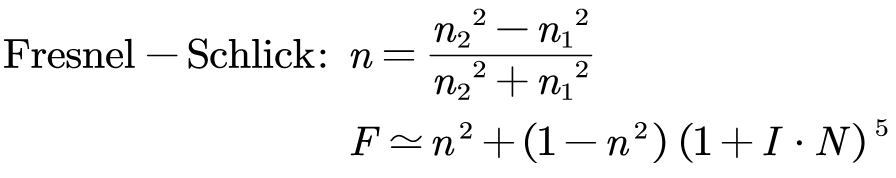
\includegraphics[width=6cm]{figure/fresnel.png}
\end{center}
$I,N$分别为入射光线的方向向量、法向量,参考后面的折射公式。当入射光线接近垂直于平面时,$I\cdot N$会接近0,于是折射效应强烈。注意以上三个值的和并不为1,需要归一化后才能用来进行采样。

然后需要计算每种情形下的光线。前两个的示意图如下:

\begin{center}
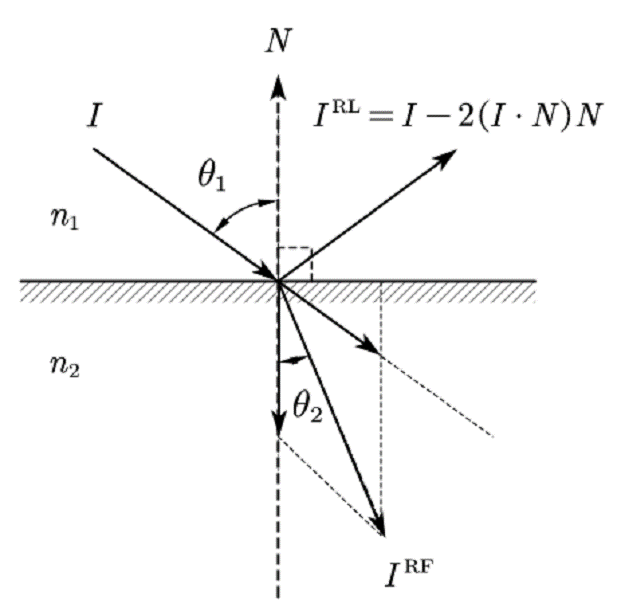
\includegraphics[width=6cm]{figure/reflection and refraction.png}
\end{center}

反射可以直接通过几何计算出来,而折射需要考虑物理效应:Fresnel效应,计算公式如下:

\begin{center}
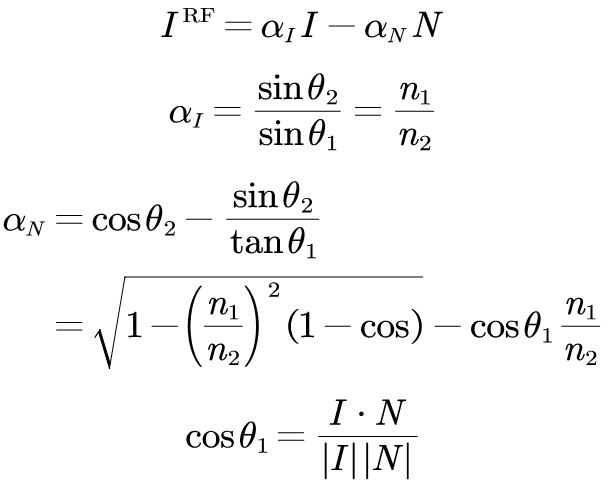
\includegraphics[width=6cm]{figure/refraction formula.png}
\end{center}

在计算漫反射时,首先建立一个局部坐标系,随机从坐标在原点的上半球上采样一点作为漫反射的采样光线,再把这条光线进行旋转、平移,使原点变换为入射光线与面片的交点,使$z$轴与面片的法向相同,公式如下:

\begin{center}
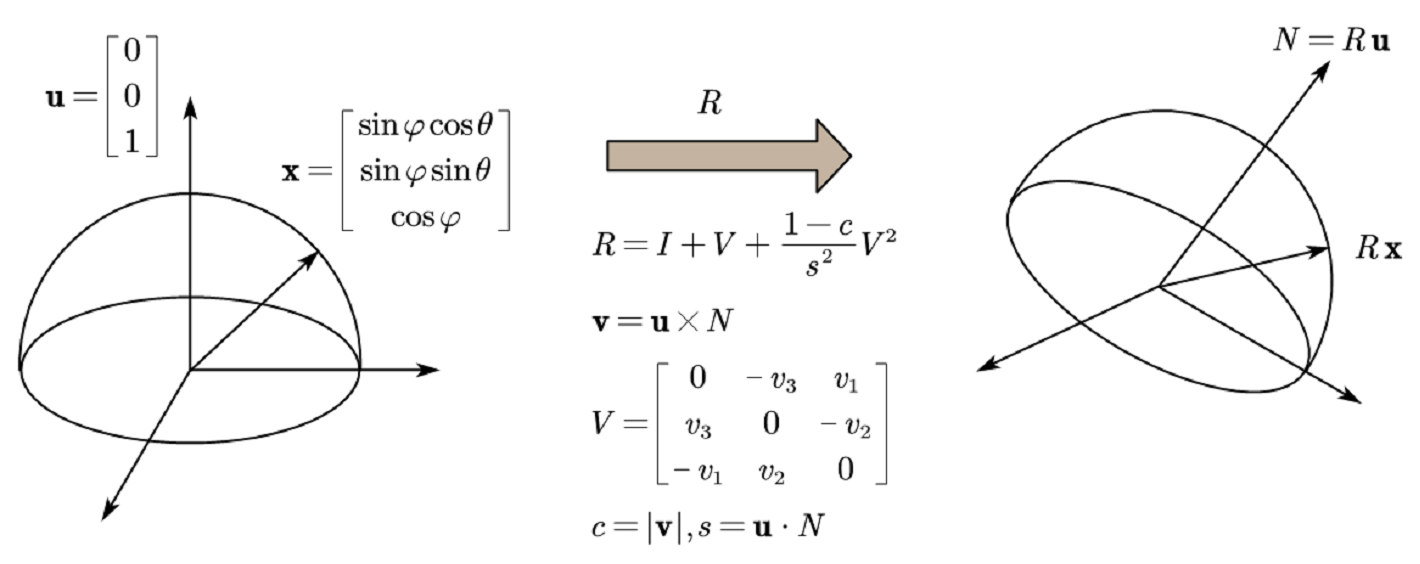
\includegraphics[width=12cm]{figure/diffuse.png}
\end{center}

然后需要确定颜色模型,即如何确定每条光线给像素的着色。本文对每条光线首先赋予一个3D向量$w=[1,1,1]^T$作为权重。此后,按以下方式在光线发生折射、反射、漫反射时更新权重:
\begin{enumerate}\label{color-model}
\item 反射:$w'=w\odot specular$
\item 漫反射:$w'=w\odot diffuse$
\item 折射:$w'=w\odot transmittance$
\item 光源:$c=w\cdot emission$
\end{enumerate}
其中$\odot$为element-wise乘法,specular、diffuse、transmittance、emission为材料的参数,$c$为最终的像素颜色。



\part{一般代数}
\chapter{多项式}

\section{多项式的性质}
\subsection{代数学基本定理}
\begin{theorem}[代数学基本定理]\label{basic-theorem-in-algebra}
每个复系数$n$次多项式$p(x)=\sum_{k=0}^{n}a_kx^k$有乘积表达式
$$p(x)=a_n(x-x_1)\cdots(x-x_n)$$
$x_k$为零点。这个定理说,每个$n$次多项式由$n$个零点和一个缩放因子$a_n$完全决定。从另一个角度来说,如果一个多项式有$n+1$个不同的零点,则它必为0。
\end{theorem}

\chapter{不等式与估计}
本章中的估计与参数估计的估计不是一回事,而是取近似一类的意思。

\section{常数不等式}
\subsection{常数列表}

\subsection{常数逼近}
$$\sqrt{7} \approx 2.6458 \leq e\approx 2.7183\leq\sqrt{8}\approx 2.828 $$

\section{基本不等式}
\begin{empheq}{align*}
    \mid |\bm{z}|-|\bm{w}|\mid \leq \mid \bm{z}-\bm{w} \mid &\leq |\bm{z}|+|\bm{w}| \mtag{三角} \\
 |\bm{x}\cdot \bm{y}|&\leq | \bm{x} | \cdot | \bm{y} |  \mtag{施瓦茨}\\
 |\bm{x}\cdot \bm{y}|&\leq \parallel \bm{x} \parallel_p \cdot \parallel \bm{y} \parallel_q \left(\frac{1}{p}+\frac{1}{q}=1\right) \mtag{Holder} \\
 \parallel \bm{x}+\bm{g} \parallel_r &\leq \parallel \bm{x}\parallel_r+\parallel \bm{y}\parallel_r\mtag{闵可夫斯基} \\
 \E(f(X))&\geq f(\E(X)),\ f\text{ convex} \label{jensen's-in-eq}\mtag{Jensen}\\
 \bm{\lambda}\cdot f(\bx)&\geq f(\bm{\lambda}\cdot \bx),\sum \lambda_i=1,\lambda_i\in[0,1],f\text{ convex}  \mtag{Jensen}
\end{empheq}
可以看出Cauchy-Schwarz不等式是Holder不等式的特例。

\section{均值不等式系列}
\subsection{基本均值不等式}
\subsubsection{公式一览}
\begin{empheq}{align}
H_n&=\frac{n}{\sum \inv{x_i}}\mtag{调和平均}\\
G_n&=\sqrt[n]{\prod x_i}\mtag{几何平均}\\
A_n&=\frac{\sum x_i}{n}\mtag{算术平均}\\
Q_n&=\sqrt{\frac{\sum x_i^2}{n}}\mtag{平方平均}\\
H_n\leq G_n&\leq A_n\leq Q_n \mtag{均值不等式}\\
G_n&\leq A_n \mtag{AM-GM不等式}
\end{empheq}
\subsubsection{应用}
\subsection{Holder不等式}
\subsubsection{公式一览}
\begin{theorem}[Holder不等式]
对于$m$个正数序列$(a_{11},a_{12},\cdots,a_{1n}),\cdots,(a_{m1},a_{m2},\cdots,a_{mn})$,有
$$\prod_i\underbrace{\sum_j a_{ij}}_{\text{列和}}\geq \left(\sum_j \underbrace{\sqrt[\uproot{18}m]{\prod_i a_{ij}}}_{\text{行几何平均}}\right)^m$$
\end{theorem}
如果取$m=2$就是柯西不等式。
\subsection{Chebyshev不等式}
\subsubsection{公式一览}
\begin{empheq}{align}
a_i,b_i\text{分别递增}, \text{则}\sum a_ib_i&\geq \inv{n}\sum a_i\sum b_i
\end{empheq}
注意不要与柯西不等式混淆。这个公式是说$\sum a_ib_i\leq \sqrt{\sum a_i^2}\sqrt{\sum b_i^2}$。

\section{积分不等式}
\subsection{基本公式}
由基本不等式可以诱导积分不等式,只要把范数运算用积分替代即可。

以下$p,q>1,\frac{1}{p}+\frac{1}{q}=1$。

\begin{empheq}{align}
	\sdet{\int_G f \dif x}&\leq \int_G\sdet{f}\dif x \mtag{三角}\\
	\sdet{\int_G fg\dif x}&\leq \sbra{\int_G\sdet{f}^p\dif x}^{1/p}\sbra{\int_G\sdet{g}^q\dif x}^{1/q} \mtag{Holder}\\
	\sdet{\int_G fg\dif x}^2&\leq \sbra{\int_G\sdet{f}^2\dif x}\sbra{\int_G\sdet{g}^2\dif x} \mtag{Schwarz}\label{int-Schwarz}\\
	\sbra{\int_G \sdet{f+g}^r\dif x}^{1/r}&\leq \sbra{\int_G\sdet{f}^r\dif x}^{1/r}+\sbra{\int_G\sdet{g}^r\dif x}^{1/r}\mtag{闵可夫斯基}\\
	\sbra{\int_G \sdet{f}^p\dif x}^{1/p}&\leq \sbra{\int_G\sdet{f}^r\dif x}^{1/r}, 0<p<r<\infty \mtag{Jensen}
\end{empheq}

\subsection{中值定理}
\subsubsection{定理}

\subsubsection{应用}
\begin{empheq}{align*}
\exists \theta\in[0,1],P(X>x)&=P(X>0)+\int_{0}^{x}\frac{1}{\sqrt{2\pi}}e^{-\frac{t^2}{2}}\dif t\\
&=\inv{2}+x\frac{1}{\sqrt{2\pi}}e^{-\frac{(\theta x)^2}{2}}
\end{empheq}

\section{函数不等式}
\subsection{基本函数}
\begin{longtable}{c}
$\forall x,y>0, xy\leq x\max(1,y^2)\leq x+xy^2 $
\end{longtable}
\section{估计技巧}
\begin{enumerate}
\item 假如两个函数在某一点处相等$f(x_0)=g(x_0)$,且当$x>x_0$时$f'(x)>g'(x)$,利用积分可知,$f(x)>g(x)$。
\end{enumerate}


\chapter{代数方程示例}
\section{多项式}
\begin{example}

\end{example}
\chapter{代数结构}

\section{代数结构一览}

\newpage
\thispagestyle{empty}
\newgeometry{left=1.5cm,bottom=0.4cm,top=0.5cm,right=1.5cm}
\begin{landscape}
\begin{tikzpicture}[grow  = right,
	sibling distance        = 6em,
	level distance          = 10em,
	edge from parent/.style = {draw, -latex},
	every node/.style       = {font=\footnotesize},
	sloped]
 \node [root] {集合}
child { node [env] {偏序集} 
		child { node [env] {格}
				edge from parent node [below] {交、并}
		}
		edge from parent node [above] {自反、传递} node[below]{反对称关系}
}
child { node [env] {半群}
		child { node [env] {幺半群}
				child { node [env] {群}
						child { node [env] {李群}
							edge from parent node [above] {解析流形} node [below] {$xy^{-1}$解析映射}
						}
						child { node [env] {交换群}
								child { node [env] {环}
										child { node (CR) [env] {除环}
												edge from parent node [above] {乘法逆元}
										}
										child { node [env] {交换环}
												child { node (F) [env] {域}
														edge from parent node  [above] {乘法逆元}
												}
												child { node [env] {$R$模}
														edge from parent node [above] {加法交换群$R$} node [below] {标量运算}	
												}
											edge from parent node [above] {乘法交换律}
										}
										edge from parent node [above] {乘法半群} node [below] {分配律}
								}
								edge from parent node [above] {(加法)交换律}
						}
						edge from parent node [above] {逆元}
				}
				edge from parent node [above] {单位元}
		}
		edge from parent node [above] {乘法封闭} node[below]{结合律} 
};
\draw[-latex] (CR) -- (F) node [pos=0.5,sloped,above] {乘法交换律};
\end{tikzpicture}

\end{landscape}
\newpage
\restoregeometry

\section{群}
\subsection{群的一般概念}
\subsubsection{群作用}
群作用是指群$G$作用于集合$\mathcal{S}$。假如对于$G$中任意元素$g$,存在$\alpha\in\mathcal{S}$,有$g\cdot \alpha \in \mathcal{S}$。则称群$G$作用于$S$。可以看出群作用其实相当于将集合$\mathcal{S}$映射为自身(或子集),即群$G$到$\mathcal{S}$的变换群内有一个同态映射$\eta$:
$$g^{\eta}\colon \alpha \rightarrow g\cdot \alpha$$
$\eta$称为群$G$在$\mathcal{S}$中的作用。

由于$\eta$是一个映射,自然地有不动点,在群论中称为核。对于$G$中某些元素,它们将$\mathcal{S}$中的元素$\alpha$映射成自身,称$G$中的这些元素为$\eta$的核。

\subsubsection{子群}
子群就是满足群性质的子集。

\paragraph{正规子群}正规子群是在共轭变换下不变的子群,即
\begin{definition}[正规子群]\label{normal-subgroup}
取$N$为一子群,若满足
$$\forall n\in N,g\in G,gng^{-1}\in N$$
则$N$是正规子群。
\end{definition}

\paragraph*{陪集}子群的完备扩张。
\begin{definition}[陪集]
	子群$H$关于$a$的左陪集为
	$$aH\coloneqq\{ax\mid x\in H\}$$
	类似地有右陪集。
\end{definition}
对于任意两个陪集$aH,bH$,它们要么相交,要么相等,因此一个群可分解为左陪集的交,或者右陪集的交,称为陪集分解。

\subsection{置换群与循环群}
\subsubsection{置换群的表示}通常用$\sigma,\pi$表示置换群(permutation),循环群是置换群表示的简化,本质上是一回事。

置换群用矩阵表示,比如
$$P=\begin{pmatrix}
1 & 2 & 3 & 4\\
1 & 3 & 2& 4
\end{pmatrix}=(1)(23)(4)$$

置换群矩阵的列表示,将第一行中的元素换成第二行中的元素,注意第一行的元素不是单纯地表示位置,而是表示特定的元素,所以交换列的顺序时,置换群是一样的。而循环群中的每个节是将前面的元素换成后面的,最后一个元素换成第一个。

\subsubsection{置换群的乘法}
注意置换群相乘时,是从右到左看的,按函数表示就是$\sigma(\pi(x))$,可以看出,内部的先算。举一个例子:
$$\begin{pmatrix}
1 & 2 & 3 &4\\
1 & 3 & 2 & 4
\end{pmatrix}\begin{pmatrix}
1 & 2 & 3 &4\\
2 & 1 & 3 &4
\end{pmatrix}=\begin{pmatrix}
1 & 2 & 3 &4\\
3 & 1 & 2 & 4
\end{pmatrix}$$

首先看第二个矩阵的第1列,表示将元素1换成2,而在第一个矩阵中,第二列将2换成3,所以1最终换成3。

\subsubsection{置换群的性质}
\paragraph*{阶数}首先转换成循环表示法, 会有若干个节,每节元素个数的最小公倍数,就是阶数。对于每个节来说,重复作用$n_i$次,会回到原来的状态,因此取最小公倍数,就表示所有节回到原来的状态。
\paragraph*{Cayley定理}每个群都与某个$\Sym(G)$的子群同构。$\Sym$是对称群,它由群$G$的所有permutation组成。也相当于说,每个群与某个置换群同构。

\subsection{商群}
商群这个概念很重要、基本,但也有点难以理解。 它相当于一个群配上等价关系:
\begin{definition}[商群]
给定群$G$和它的正规子群$N$,定义商群$G/N$为$N$在$G$中的所有左陪集,或者:
$$G/N\coloneqq \{aN\in G  \}$$
商群中的乘法定义为
$$(aN)(bN)\coloneqq (ab)N$$
由于$N$是正规子群,所以取$aN$或者$Na$是一回事。
\end{definition}

\subsection{群的例子}
\subsubsection{线性群}
\begin{longtable}{ccc}
	\toprule
	表示& 含义 &维数\\
	\midrule
	$\GL(n,F)$ &$F$上全体可逆矩阵& $n^2$\\
	$\SL(n,F)$ &$F$上全体行列式为1的可逆矩阵&$n^2-1$\\
	$\text{O}(n,F)$ & $\GL(n,F)$中的正交矩阵&\\
	$\text{SO}(n,F)$ & $\SL(n,F)$中的正交矩阵&\\
	\bottomrule
\end{longtable}

\section{环}

\section{域}

\section{特殊代数结构的例子}

\subsection{Tropical Geometry}
属于代数几何的一种.
\begin{definition}{Tropical Geometry}{}
\begin{empheq}{align*}
x\oplus y&=\max (x,y)\\
x\odot y&=x+y\\
x^a&=ax\\
\bx^{\bm{a}}&=c\odot x_1^{a_1}\odot\cdots\odot x_d^{a_d}\mtag{Tropical monomial}\\
f(\bx)&=c_1\bx^{\bm{\alpha}_1}\oplus\cdots\oplus\bx^{\bm{\alpha_r}}\mtag{Tropical Polynomial}\\
f(x)\oslash g(x)&=f(x)-g(x)\mtag{Rational Function}
\end{empheq}

\end{definition}


前两个算子可以构成半环$\mathbb{T}\coloneqq (\mathbb{R}\cup\{-\infty\},\oplus,\odot)$.这里的$\max$也可以换成$\min$,两者等价.

\chapter{代数几何}
\section{基本概念}

\begin{definition}{层}{}
	
\end{definition}

\begin{definition}{概型}{}
	
\end{definition}

\begin{definition}{纤维丛}{}
	
\end{definition}

\begin{definition}{层}{}
	
\end{definition}
\chapter{范畴结构}\label{category}
一个范畴由对象及对象之间的联系(态射)构成,所以它本身也属于一种结构,但又不同于一般的代数结构,范畴可以视为结构的结构,描述了不同具体结构(集合结构、群结构等等)的共性。所以本章冠以“结构”的名字。

也有人认为,集合是从元素的角度来理解世界,而范畴论是从关系的角度来理解世界。

范畴论中经常使用交换图的描述方式,交换图的含义是说,对于图中给定的起点与终点,任意一条从起点到终点的路径都是成立的,即经过不同的计算可以从起点到达相同的终点。

\section{基本定义}
\subsection{范畴}
\begin{definition}[范畴]
范畴由如下组成:
\begin{enumerate}
\item 对象$A,B,C,\cdots$组成的类$\obj(\mathcal{C})$。
\item 任意两个对象$A,B$,存在从$A$到$B$的态射$\mathcal{C}(A,B)$(也morphism,可记为$\Hom_{\mathcal{C}}(A,B)$),元素记为$f\colon A\rightarrow B$。
\item (复合)对任意三个对象$A,B,C$,存在映射$\mathcal{C}(A,B)\times \mathcal{C}(B,C)\rightarrow \mathcal{C}(A,C),(f,g)\mapsto gf$,并且满足:
\begin{enumerate}
	\item (惟一性)集合$\mathcal{C}(A_1,B_1)$与$\mathcal{C}(A_2,B_2)$相同当且仅当$A_1=A_2,B_1=B_2$。
	\item (结合律)对态射$f\colon A\rightarrow B,g\colon B\rightarrow C,h:C\rightarrow D$,有$h(fg)=(hg)f$。
	\item (单位元)对每个对象$A$,有态射$1_A\colon A\rightarrow A$,使得对任意$f\colon A\rightarrow B,g\colon C\rightarrow A$有$f1_A=f,1_Ag=g$。
\end{enumerate}
\end{enumerate}
\end{definition}

在以上的定义中,注意,“态射”可以理解为一般的“映射”。
\subsection[函子]
简单地说,函子是从一个范畴到另一个范畴的映射,通常分为共变函子与反变函子。

\begin{definition}[共变与反变函子]
给定两个范畴$\mathcal{C,D}$与范畴间的函子$F\colon \mathcal{C}\rightarrow\mathcal{D}$,如果$\mathcal{C}$中每一个对象$A$,对应$\mathcal{D}$中的$F(A)$,$\mathcal{C}$中每一个态射$f\colon A\rightarrow B$对应$F(f)\colon F(A)\rightarrow F(B)$,且
\begin{enumerate}
	\item $F(1_A)=1_{F(A)}$。
	\item $F(gf)=F(g)F(f)$。
\end{enumerate}
则称$F$为从$\mathcal{C}$到$\mathcal{D}$的共变函子。以上条件如果变成$F(f)\colon F(B)\rightarrow F(A),F(gf)=F(f)F(g)$,则称之为反变函子。
\end{definition}

从形式上看,“共变”与“反变”像是在说分配律的顺序。
\subsection{范畴的例子}

\section{高阶范畴}


\section{范畴论的应用}

\chapter{同伦论}
\chapter{同调论}

\part{线性代数}\label{linear-algebra-part}
\chapter{矩阵定理}

\section{向量性质}

\subsection{基本性质}

\paragraph*{内积与夹角}在二维平面上,内积的含义是平行四边形的有向面积.

$$\cos\theta=\frac{\bx\cdot\by}{|\bx||\by|}$$

$\theta$为夹角.夹角与欧几里得距离有关联.考虑端点在单位圆上的两个向量$\bx_1,\bx_2$.则两个端点的欧几里得距离为:

$$2\sin\frac{\theta}{2}=2\sqrt{1-\cos^2\frac{\theta}{2}}$$

参考下图:

\begin{center}
	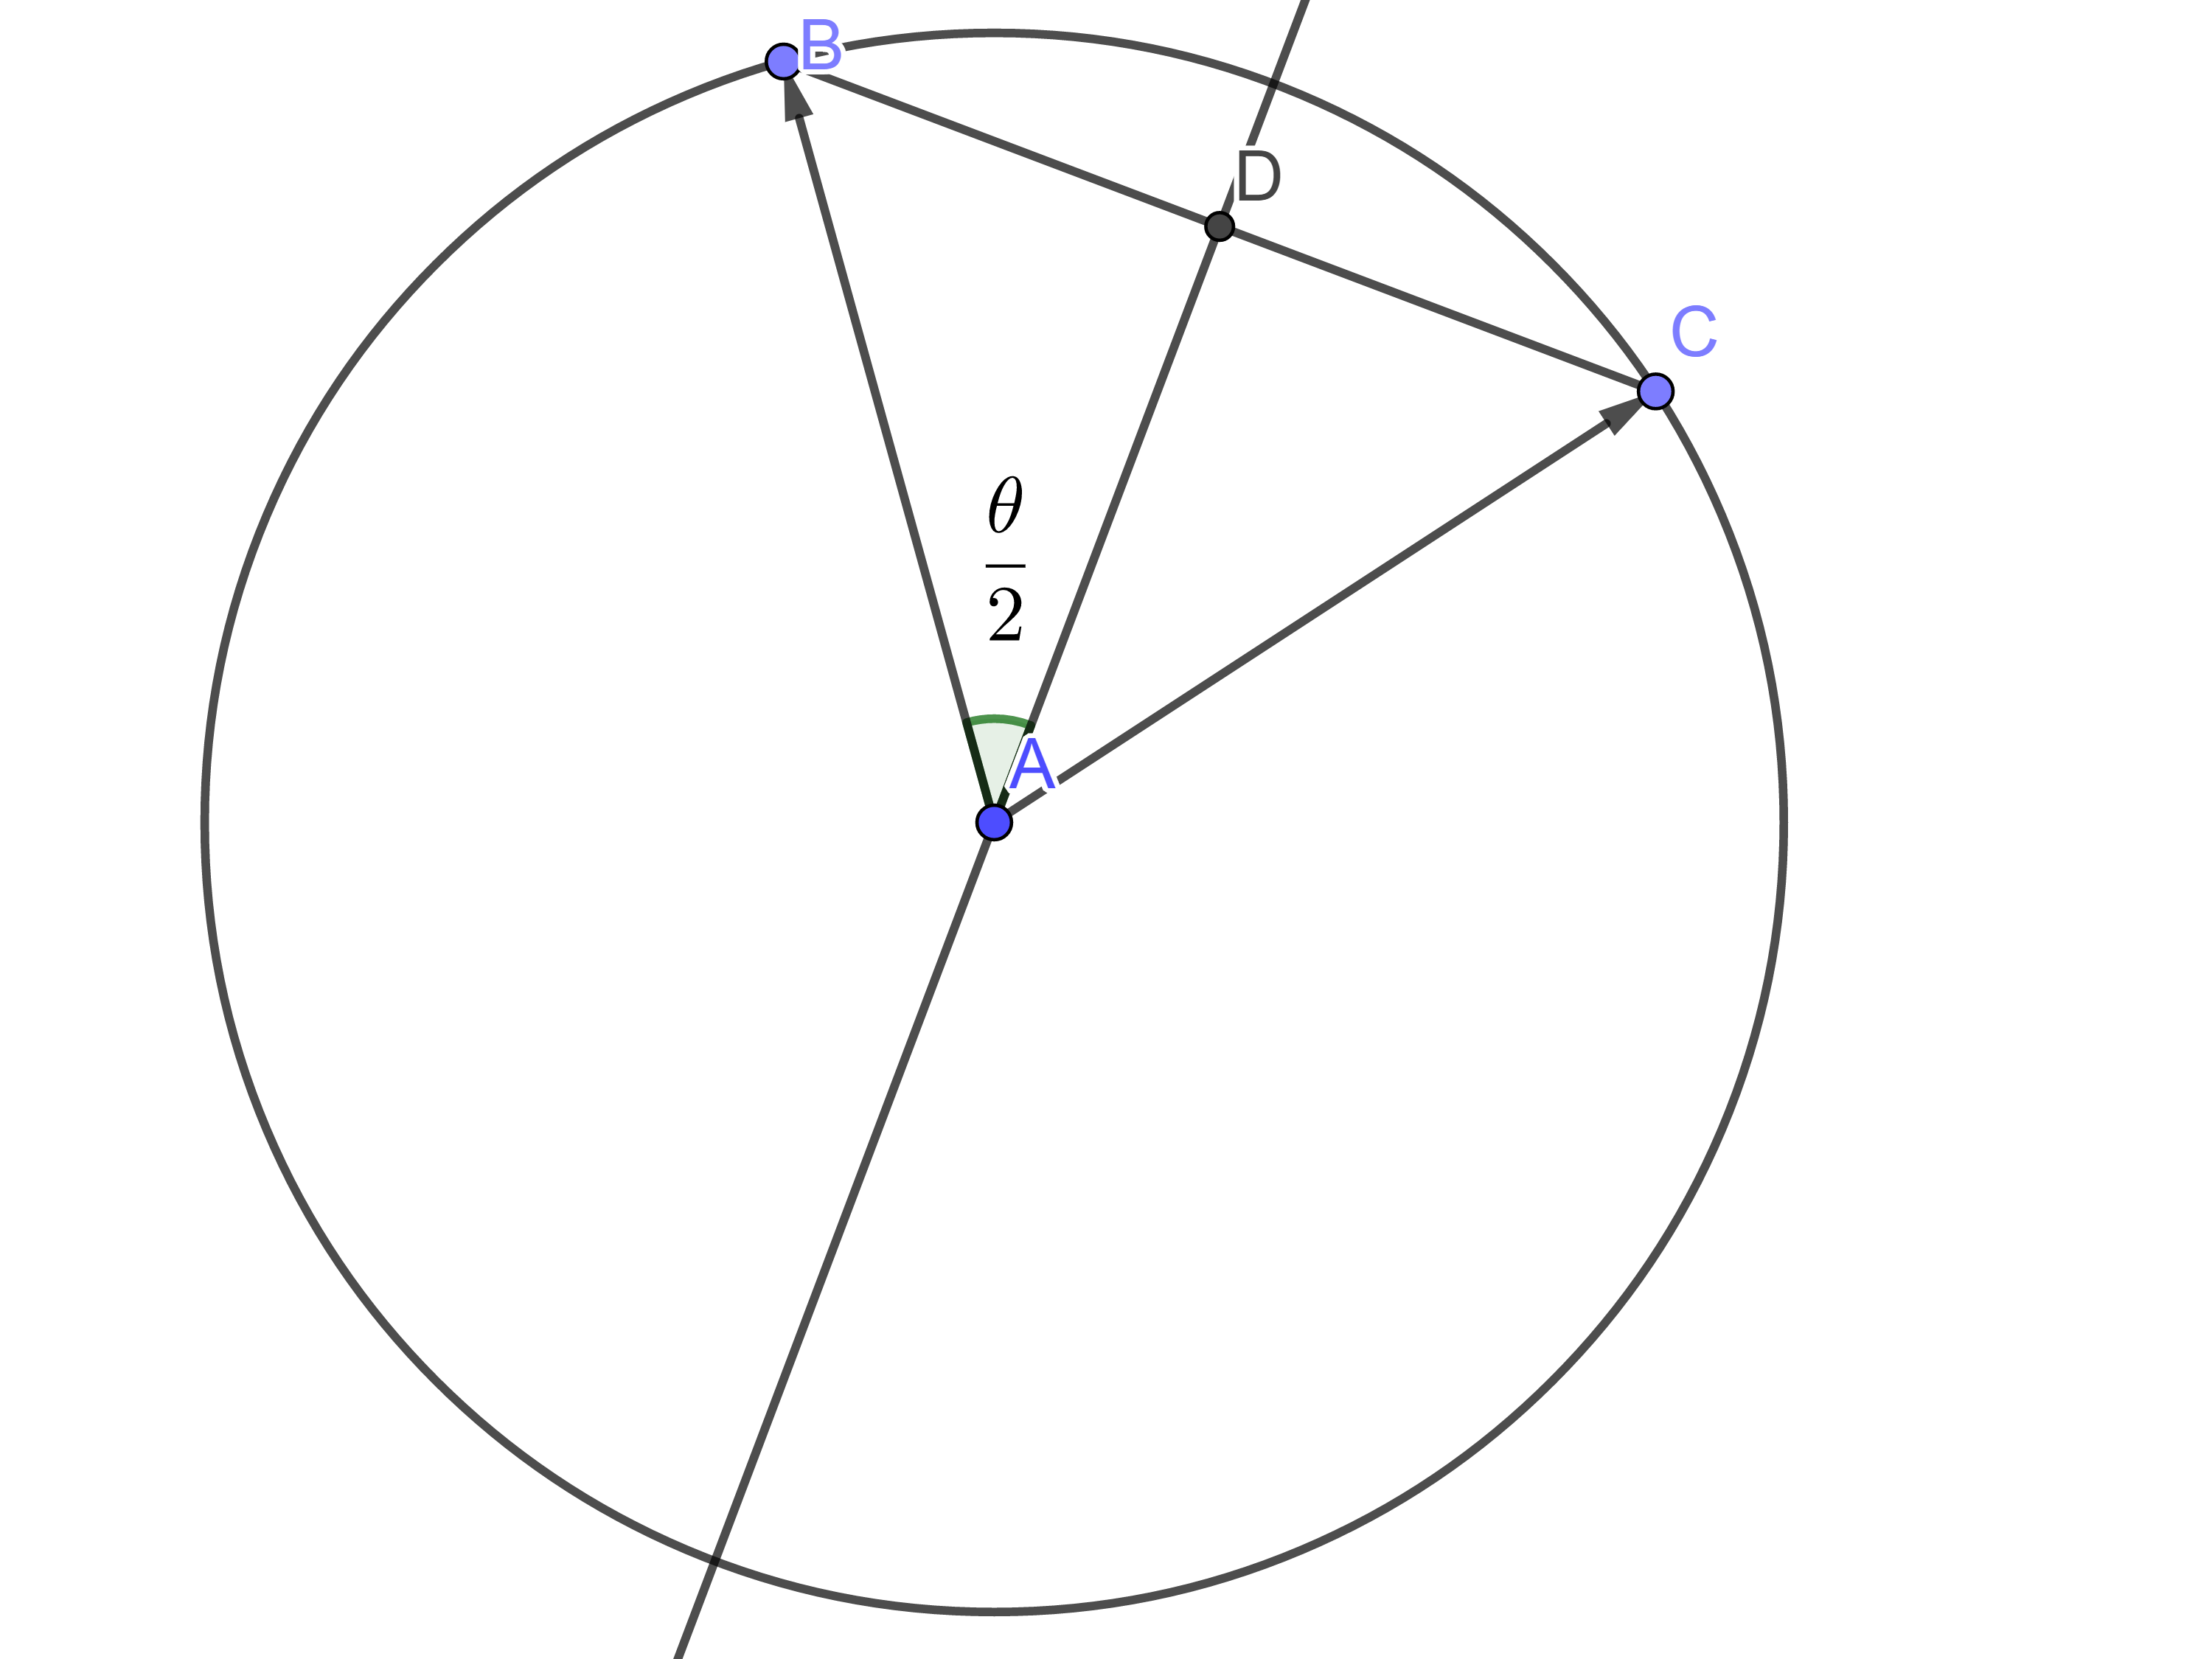
\includegraphics[width=6cm]{figure/cosDistance.png}
\end{center}

\paragraph*{垂直(orthogonal)}垂直关系可以用内积描述:

$$\bx\cdot\by=0$$

如果另外有$|\bx|=|\by|=1$,则称为orthonomal.
\section{矩阵性质}

\subsection{逆矩阵}
$$A^{-1}=\frac{1}{|A|}A^{\star}$$
其中$A^{\star}=M^T$为伴随矩阵,其值为
$$M_{ij}=(-1)^{i+j}|A_{-i,-j}|$$
$M_{-i,-j}$为去掉矩阵的$i$行$j$列后剩下的矩阵。

$n$阶可逆矩阵构成一般线性群$\GL_n$。对于2阶矩阵有简单的表达式:
$$\begin{bmatrix}
a&b\\c&d
\end{bmatrix}=\frac{1}{ad-bc}\begin{bmatrix}
d&-b\\-c&a
\end{bmatrix}$$
注意
$$M=\begin{bmatrix}
	d&-c\\-b &a
\end{bmatrix}$$
转置一下就是上面的表达式。求二阶线性方程组的时候可以用。

手动计算矩阵逆时可以使用消元法,首先构造矩阵$(A,I)$,通过行变换变成$(I,A')$,则$A'=A^{-1}$。具体操作时,首先把$A$的下半部分变成全0,依次把第1列的$2,\cdots,n$行元素变成0,然后把第2列的$3,\cdots,n$个元素变成0,$\cdots$再变换上半部分为全0。
\subsection{特征向量与特征值}
\subsubsection{定义}
特征值集合在算子理论中也叫做谱,用$\sigma(A)$表示,通常将特征值从大到小排列,那么$\lambda_1=\sigma_1(A)$就表示最大的特征值,$\lambda_n=\sigma_n(A)$为最小特征值。常用的特征值只对\textbf{方阵}才有定义。

\begin{empheq}{align*}
	A\bx&=\lambda\bx\\
	\sum \lambda_i &=\trace A\\
	\prod \lambda_i &=\det A
\end{empheq}

特征值的最大模就是谱半径:

\begin{definition}[谱半径]\label{matrix-spec-radius}
\begin{equation}
\rho(A)=\max_i |\lambda_i(A)|
\end{equation}
\end{definition}
要注意区别谱半径与谱范数,谱半径不是矩阵范数,但它非常重要。

谱半径有一个重要性质:
$$\rho(A)\leq\|A\|$$
即它小于任意一种范数。同时还有Gelfand定理:
\begin{equation}
\rho(A)=\lim_{k\rightarrow \infty} \|A^k\|^{1/k}
\end{equation}

\subsubsection{特征值和特征向量性质}
\begin{enumerate}
\item  常见矩阵函数的特征值:
\begin{longtable}{|c|c|c|c|c|}
\hline
矩阵& $A$& $A^T$& $A^{-1}$& $A^k$\\
\hline
特征值& $\lambda$ & $\lambda$ & $\inv{\lambda}$ & $\lambda^k$\\
\hline  
\end{longtable}
如果$A$有SVD分解$A=U\Lambda V$,即$A$有奇异值$\sigma_i$,则$AA^T$的特征值为$\lambda_i=\sigma_i^2$。
\item 如果已知特征值和特征向量,则从$A$中去掉一行,右边的特征向量中去掉对应的行,等式依然成立.
\item 假设$A\in\mathbb{R}^{d\times n},B\in\mathbb{R}^{n\times d},d\leq n$,即$A$为横矩阵,则$AB$为小方阵,有$\sigma(BA)=(\sigma(AB),\bm{0})$,特别地,假如$d=n$,那么$\sigma(AB)=\sigma(BA)$。

对于三个矩阵,在矩阵乘法成立的情况下,有$\sigma(ABC)=\sigma(BCA)=\sigma(CAB)$。在二次型定理\ref{quadratic-form-ratio}的证明中就会用到:
$$\sigma(B^{-1}A)=\sigma(R^{-1}(R^{-T})A)=\sigma(R^{-T}AR^{-1})$$
\item 如果$A$是Hermitian矩阵,则
\begin{empheq}{align}
\lambda_1&=\max_{\|\bx\|=1}\bx^TA\bx\\
\lambda_n&=\min_{\|\bx\|=1} \bx^TA\bx\\
\end{empheq}

更一般地有:
\begin{empheq}{align}
\sum_{i=1}^k \lambda_k&=\underset{(\bx_1,\cdots,\bx_k)}{\max}\sum_{i=1}^{k}\bx_i^TA\bx_i \mtag{Ky Fan's Maximum Principle}\\
\sum_{i=n-k+1}^n \lambda_k&=\underset{(\bx_1,\cdots,\bx_k)}{\min}\sum_{i=1}^{k}\bx_i^TA\bx_i \mtag{Ky Fan's Maximum Principle}\\
\end{empheq}
要求$(\bx_1,\cdots,\bx_k)$相互orthonormal。
\end{enumerate}

\subsubsection{迭代算法}
\paragraph*{计算最大的特征值与特征向量}
\begin{empheq}{align}
\bx_{n+1}&=\alpha(A\bx-\bx^T\bx\bx)+\bx
\end{empheq}
收敛时$\bx$就是特征向量,对应特征值$\bx^T\bx$。

\paragraph*{计算最小的特征值与特征向量}
\begin{empheq}{align}
\bx_{n+1}&=\alpha((kI-A)\bx-\bx^T\bx\bx)+\bx
\end{empheq}

\subsection{奇异值}
SVD分解中$\Lambda$矩阵的对角元素就是奇异值。

\subsubsection{与特征值的联系}
\begin{enumerate}
\item 
$$\sigma_i^2(A)=\lambda_i(A^*A)=\lambda(AA^*)$$
\item 对于$n$阶矩阵:
$$\lambda_i(A+A^*)\leq 2\sigma_i(A)$$

假如$A$是对称的,则有
$$\lambda_i(A)\leq\sigma_i(A)$$
\item 正定矩阵的特征值与奇异值相同。
\end{enumerate}
\subsubsection{$A+B$的奇异值}
\begin{enumerate}
\item $A+B,A,B\in\mathbb{C}^{m,n}$的奇异值:
$$\sigma_{i+j-1}(A+B)\leq \sigma_i(A)+\sigma_j(B),i+j-1\leq \min\{m,n\}$$

特殊情况:
\begin{enumerate}
\item 假如取$m=n$,分别令$i=1,j=n$和$i=n,j=1$,有:
\begin{empheq}{align*}
\sigma_n(A+B)\leq \sigma_1(A)+\sigma_n(B)\\
\sigma_n(A+B)\leq \sigma_n(A)+\sigma_1(B)\\
\end{empheq}
\end{enumerate}
\end{enumerate}

\subsection{矩阵范数}
矩阵范数对任何矩阵均存在,且任何矩阵范数都是等价的。

\subsubsection{范数的类型}
\paragraph*{Unitarily invariant norm}比较常用的类型。
\begin{definition}[Unitarily invariant norm]
一个范数如果满足
$$\forall A,\|UAV\|=\|A\|$$
其中$U,V$为任意酉矩阵。则称之为Unitarily invariant norm。

Frobenius范数都属于此类。
\end{definition}

\subsubsection{诱导范数}
参考算子范数\ref{op-norm},它依赖于向量的范数。如果向量取$p$范数,则有相应的$\|A\|_p$。特殊情形:
\begin{description}
\item[$p=1$] 列范数,先把所有元素取绝对值,再对每列求和,然后取最大的。
\item[$p=2$] 谱范数,参见\ref{matrix-spec-norm}。
\item[$p=\infty$] 行范数。与列范数相对应。
\end{description}
\subsubsection{谱范数}
\begin{definition}[谱范数]\label{matrix-spec-norm}
$$\|A\|_2=\sigma_{\max}(A^TA)$$
即最大奇异值。注意$A$不必是方阵。
\end{definition}
\begin{property}
\begin{enumerate}
\item 根据奇异值分解可得:
$$\|A^{-1}\|=\inv{\min \sigma(A)}$$
\end{enumerate}
\end{property}

\subsubsection{Frobenius范数}
\begin{definition}[Frobenius范数]
对于一个长方阵$X\in\mathbb{R}^{n\times d}$,有Frobenius范数:
\begin{empheq}{equation}
\|A\|_F=\sqrt{\trace(A^TA)}=\sqrt{\trace(AA^T)}=\sqrt{\sum |A_{ij}|^2}
\end{empheq}
最后一个等号说把所有元素排列一个向量,然后取向量的$L_2$范数。

显然从定义可以看出
$$\|A\|_2\leq \|A\|_F$$
\end{definition}

\subsection{特殊矩阵}
\subsubsection{常见复矩阵及对应的实矩阵}
记$A^H$为伴随矩阵,是复矩阵的共轭转置、实矩阵的转置($A^T$),有时也用$A^*$表示.

\begin{longtable}{c c}
	\toprule
	名称& 定义 \\
	\midrule
	Hermitian(对称矩阵) &$A=A^H$ \\
	斜伴矩阵(反对称矩阵)&$A=-A^H$\\
	正规矩阵& $AA^H=A^H A$\\
	酉矩阵(正交矩阵)& $AA^H=A^H A=I$\\
	\bottomrule
\end{longtable}

\paragraph*{Hermitian}具有非常重要的性质:
\begin{enumerate}
\item 如果元素全为实数,则为实对称阵。满足性质:
\begin{enumerate}
\item 实对称矩阵必然可以对角化。
\item 不同特征值对应的特征向量正交。
\item 特征值必为实数。
\end{enumerate}
\end{enumerate}
\subsubsection{正矩阵与非负矩阵族}
\paragraph*{非负矩阵}元素非负的矩阵,不要与负定矩阵混淆。

\begin{definition}[非负矩阵]
对于矩阵$A$,如果$A_{ij}\geq 0$,称$A$为非负矩阵,记为$A\geq 0$。我们用$|A|$表示按元素取绝对值。

非负矩阵具有以下性质:
\begin{enumerate}
\item 如果$B\geq A\geq 0,D\geq C\geq 0$,则$BD\geq Ac\geq 0$
\item 如果$B\geq A\geq 0$,则$B^k\geq A^k\geq 0,k=1,2,\cdots$。
\item 如果$|A|\geq B$,则$\rho(A)\leq\rho(|A|)\leq \rho(B)$。
\end{enumerate}
\end{definition}


\paragraph*{Z矩阵与M矩阵}
\begin{definition}[Z矩阵与M矩阵]\label{z-m-matrix}
记方阵$A=[A_{ij}]\in\mathbb{R}^{n\times n}$,如果$A_{ij}\leq 0,i\neq j$(非对角元素小于等于0),则称$A$为$Z$矩阵,任何一个$Z$矩阵$A$可以表示成$A=sI-B$,且$s>0,B\geq 0$。

如果$s\geq \rho(A)$,称$A$为$M$矩阵。若$s>\rho(B)$,称之为非奇异$M$矩阵,$s=\rho(B)$时,称为奇异的$M$矩阵。

$\rho(A)$为谱半径\ref{matrix-spec-radius}。
\end{definition}

\begin{theorem}[Z矩阵的性质]
若$A$为$Z$矩阵,则下列命题等价:
\begin{enumerate}
\item $A$是非奇异的$M$矩阵。
\item $A$非奇异且$A^{-1}\geq 0$。
\item 存在$\bx>0$使得$A\bx>0$。
\item 任意$\lambda\in\lambda(A)$,有$\Re(\lambda)>0$。即特征值的实部为正。
\item $A$的所有实特征值都是正数。
\end{enumerate}
\end{theorem}
\subsubsection{正定矩阵与二次型}
\paragraph*{定义}
\begin{definition}[正定矩阵]\label{pos-definite-matrix}
对称矩阵$A$如果满足
$$\forall \bx\in\mathbb{R}^n,\bx^TA\bx> 0$$
称$A$为正定矩阵,如果取$\geq$,就是半正定矩阵,如果取$<$,就是负定矩阵。,单位阵是半正定矩阵。

正定矩阵也可以表示为$A\succ 0$,半正定矩阵就是$A\succeq 0$。有的地方也用$A\geq 0$来表示半正定矩阵,但这容易与非负矩阵混淆。

\end{definition}
\paragraph*{性质}正定矩阵满足以下性质:
\begin{enumerate}
\item 行列式为正。这是由于特征值非负,特征值的乘积就是行列式。
\item 对角线元素之和为正。因为特征值之和为对角线元素之和。
\item 特征值全部为正。
\item 正定矩阵之和仍然正定,Hadmond积也正定(Schur乘积定理),但矩阵乘积\textbf{可能不正定}:
\begin{empheq}{equation}
A\succ 0,B\succ 0\implies A+B\succ 0, A\odot B\succ 0
\end{empheq}
\item 正定矩阵的逆正定:$A\succ 0\implies A^{-1}\succ 0$。再加上上一条,可以导出:如果$A\succ B\succ 0$,则$A+B\succ B$,然后有$(A+B)^{-1}\succ B^{-1}$。
\item 对于两个正定矩阵$A,B$,有和矩阵的特征值:
$$\lambda_k(A)+\lambda_n(B)\leq \lambda_k(A+B)\leq \lambda_k(A)+\lambda_1(B)$$
$\lambda_1$为最大的特征值,$\lambda_n$为最小特征值。特殊情况:
\begin{empheq}{align*}
\lambda_n(A)+\lambda_n(B)&\leq \lambda_n(A+B)\leq\lambda_n(A)+\lambda_1(B)
\end{empheq}

有矩阵乘法的特征值:
\begin{empheq}{align*}
\lambda_1(AB)&\leq \lambda_1(A)\lambda_1(B)\\
\lambda_n(A)\lambda_n(B)&\leq \lambda_n(AB)
\end{empheq}
\end{enumerate}


涉及正定或者半正定矩阵的其它一些定理:
\begin{enumerate}
\item 如果$A$非负定,则
$$(\bx^TA\by)^2\leq(\bx^TA\bx)(\by^TA\by)$$
\item 如果$A$正定,则
$$(\bx^T\by)^2\leq (\bx^TA\bx)(\by^TA^{-1}\by)$$
\item 如果$A$非负定,则
$$|A_{ij}|\leq \max \{A_{ii}\}$$
也就是说非负定矩阵中绝对值最大的元素位于对角线上。
\item 非负定矩阵$A,B$满足:
\begin{empheq}{align}
0\leq \trace(AB)&\leq \trace(A)\trace(B)\\
\det(A+B)&\geq \det(A)+\det(B) 
\end{empheq}
对于第2式,如果$n\geq 2$且$A,B$正定,则只取$>$。
\item 如果$A,B,C,D,U,V$都是同样大小的方阵,且$U,V$正定,则
$$\det(AUA^T+BVB^T)\det(CUC^T+DVD^T)\geq \det(AUC6T+BVD^T)^2$$
\item 如果$A$非负定,则
$$\det(I+A)\geq 1+\det(A)$$
如果$n\geq 2$且$A$正定,则只取$>$。
\end{enumerate}

\paragraph*{判定}判断一个对称矩阵是否正定:
\begin{enumerate}
\item 顺序主子式为正。就是取前$k$行$k$列,计算行列式。左上角元素就是第1个顺序主子式,所以要求这个元素为正。

如果奇数阶主子式为负(第一个元素为负),偶数阶为负,就是负定矩阵。

此外需要注意,假如顺序主子式全部非负,不一定半正定。
\end{enumerate}

\paragraph*{二次型}
\begin{enumerate}
\item 对于任意对称方阵$A$,
\begin{empheq}{align*}
\max_{|bx|=1}\bx^TA\bx=\lambda_{\max},&\quad \min_{|bx|=1}\bx^TA\bx=\lambda_{\min}\\
\max_{bx}\frac{\bx^TA\bx}{\bx^T\bx}=\lambda_{\max},&\quad \min_{bx}\frac{\bx^TA\bx}{\bx^T\bx}=\lambda_{\min}\\
\end{empheq}
\item\label{quadratic-form-ratio} $A,B$为任意$n$阶方阵, $B$正定,则有
$$\max_{\bx\neq\bm{0}} \frac{\bx^TA\bx}{\bx^TB\bx}=\lambda_{\max}(B^{-1}A)$$

\end{enumerate}
\subsubsection{投影矩阵}
给定一个行满秩矩阵$A\in \mathbb{R}^{m\times n},m\leq n$,现在有一个向量$\bx\in\mathbb{R}^n$,希望将它投影到$A$的零空间。

首先可以这样考虑,求一个向量$\bx'$,它满足零空间的定义,同时尽量接近$\bx$,可以形式化为一个最小二乘问题:
\begin{empheq}{equation}
\begin{aligned}
	\min_{\bx'\in\mathbb{R}^n} & \inv{2}(\bx'-\bx)^T(\bx'-\bx)\\
	\text{s.t. }& A\bx'=\bm{0}
\end{aligned}
\end{empheq}
目标函数是距离。用乘子法:
\begin{empheq}{align*}
L(\bx',\bm{v})&=\inv{2}(\bx'-bx)^T(\bx'-\bx)+\bm{v}^TA\bx',\bm{v}\in\mathbb{R}^m\\
\pdv{L}{\bx'}&=\bx'-\bx+A^T\bm{v}=0\\
A\bx'&=\bm{0}
\end{empheq}
第二个式子左乘$A$,就可以得到
$$\bm{v}=(AA^T)^{-1}A\bx$$

同时由第二个式子有$\bx'=\bx-A^T\bm{v}$,于是
$$\bx'=P\bx=(I-A^T(AA^T)^{-1}A)\bx$$
$P=I-A^T(AA^T)^{-1}A,P\in\mathbb{R}^{n\times n}$称为投影矩阵。

也可以从另一个角度考虑,希望求解$\bx$在$A$的零空间下的坐标。

\subsubsection{Stiefel流形}
Stiefel流形是正交矩阵的扩展,它的定义为
\begin{empheq}{equation}
\mathcal{S}_{n,d}\{A\in\mathbb{C}^{n\times d}:A^HA=I\}
\end{empheq}
注意它不必是方阵。

\paragraph*{性质}Stiefel流形具有以下性质:
\begin{enumerate}
\item $\dim(\mathcal{S}_{n,d})=nd-\inv{2}d(d+1)$
\end{enumerate}

\subsection{矩阵分解}
\subsubsection{概览}
\begin{longtable}{m{0.15\textwidth} m{0.15\textwidth} m{0.3\textwidth} m{0.4\textwidth}}
	\toprule
	\hfil \textbf{范围}&\hfil \textbf{名称} & \hfil \textbf{形式}  & \hfil \textbf{说明}\\
	\midrule
任意矩阵 &	SVD分解 &$A_{m\times n}=U_{m\times m}\Lambda_{m\times n}V_{n\times n}$&$U,V$酉矩阵,$\Lambda$实对角阵,其中的元素为奇异值。\\
任意方阵&Jordan标准型 &$A=PJP^{-1}$ &$J=\diag(J_1,J_2,\cdots)$,其中$J_k$的对角线上全为$\lambda_k$,且对角线右边的一个元素全为1。形如:
$$J_k=\begin{bmatrix}
\lambda_k & 1 & &\\
& \lambda_k& 1 & & \\
& & \cdots& &\\
& & & &\lambda_k
\end{bmatrix}$$ \\
\hline
	任意方阵 &QR分解&$A=QR$ & $Q$正交,$R$上三角\\
    \hline
某些方阵& 对角化 &$A=Q\Lambda Q^{-1}$&$\Lambda$为对角矩阵,对角线上元素为特征值。$Q$的列为特征向量,显然如果要$Q$可逆,则特征空间的维数必然等于$n$。

强调实对称矩阵必然可以对角化。\\
\hline
    任意方阵& Schur分解 &$A=QUQ^{H}$ & $Q$酉矩阵,因此 $Q^{-1}=Q^H$,$U$半上三角阵,对角线上为$A$的特征值.\\
    \hline
	半正定矩阵& Cholesky分解& $A=LL^H $& $L$下三角.\\
	\bottomrule
\end{longtable}

\subsubsection{SVD分解}
\paragraph*{低秩逼近}SVD分解的一个重要应用是用低秩矩阵逼近一个目标矩阵,其最优逼近为
$$A_k=\sum_{i=1}^k\lambda_i \bm{u}_i\bm{v}_i^T$$
$\bm{u}_i$是$U$的列,$\bm{v}_i$是$V$的列。
\section{线性方程组的解}
\subsection{齐次方程组}
一个齐次线性方程组形如:
$$A\bx=\bm{0}$$
$A\in \mathbb{R}^{m\times n}$,$m$是方程个数,$n$是变量个数。
\begin{enumerate}
\item 显然,这个方程组至少有1个解:$\bm{0}$解,即$\bx=\bm{0}$。
\item 假如$\rank(A)=n$,即列满秩,则只有$\bm{0}$解。列满秩时,列之间是独立的,所以不可能找到一个线性组合使和为0.
\item 假如$\rank(A)<n$,则有无穷多个解。此时解空间又称为$\nullspace$(或者叫kernel),满足条件:
$$\dim(\nullspace(A))+\rank(A)=n$$
零空间的基相当于方程组基础解系,$\dim(\nullspace(A))$就是基变量的个数。
\end{enumerate}
\subsection{非齐次方程组}
对于一个非齐次方程组
$$A\bx=\bm{b}$$
其增广矩阵为$(A,\bm{b})$。解的存在性由以下判别方法给出:
\begin{enumerate}
\item $\rank(A)< \rank(A,\bm{b})$,则无解。
\item $\rank(A)= \rank(A,\bm{b})<n$,有多个解。
\item $\rank(A)= \rank(A,\bm{b})=n$,唯一解。
\end{enumerate}
\chapter{矩阵代数}

\section{基本矩阵运算}
%\subsection{公式}
\subsection{矩阵乘法与基本算子}
\paragraph*{核心原理}
\begin{empheq}{align*}
	\bm{x}^T\bm{y}&=\bm{y}^T\bm{x}=\text{trace}(\bm{x}\bm{y}^T)\\
	\by^T\bx\bx^T\by&=(\bx^T\by)^2=(\by^T\bx)^2\\
    \bx^TA\by&=\trace(\by\bx^TA)\\
	\text{trace}(AB)&=\text{trace}(BA)\\
	\trace(ABC)&=\trace(BCA)=\trace(CBA)\\
	\det(A^{-1})&=\det(A)^{-1}\\
	\det(e^A)&=e^{\trace(A)}\\
	\det (I_m+AB^T)&=\det (I_n+A^TB)\\
	\det(I+\bm{a}\bm{b}^T)&=1+\bm{a}^T\bm{b}\\
	\det (I+A)&=1+\det A+\text{trace}(A)\\
	\det(I+\varepsilon A)&\approx 1+\det(A)+\varepsilon\trace(A)+\inv{2}\varepsilon^2\trace(A)^2-\inv{2}\varepsilon^2\trace(A^2)\\	\det\left(A^{-1}+A^{-1}BA\right)&=\det\left(A^{-1}A^{-1}A++A^{-1}BA\right)=\det\left(A^{-1}+B\right)\\
\det \begin{bmatrix}
A&B\\C&D\\
\end{bmatrix}&=\det (A)\det(D-CA^{-1}B)\\
 &=\det (D)\det(A-BD^{-1}C)
\end{empheq}
以上假定$\diag$是列向量。

矩阵运算如果在运算过程中产生了标量,那么不一定满足结合律,比如:
$$\bx^T\bx\bx\neq \bx^T(\bx\bx)$$

右边是没有定义的.但是假如没有生成标量,那么就是结合的.这是因为标量乘以矩阵,实际上是两个元素,无法进一步化简了;而多个矩阵乘起来,最终得到一个矩阵,只有一个元素.

此外还要强调:
\begin{empheq}{align*}
ABA+ACA&=A(B+C)A\\
ACB+DCE&\neq (A+D)C(B+E)
\end{empheq}

后面这个地方比较容易出错。

矩阵运算中,要注意几点:

\begin{enumerate}
	\item 假如包含标量,可以放到前面或者后面、可以转置.标量非常重要的,要注意区分.
	\item 注意一些基本的量,可能隐含一些潜在的关系,比如求值使两个向量相减为0,则向量是平行的,正交回归是一例.
	\item 在式子中插入一个单位项$I=AA^{-1}=A^{-1}A$用于构造二次型,在多元高斯分布的计算中比较常用。
	\item 掌握一些改写方程的技巧:
	
		\begin{empheq}{align*}
			1+\bm{\theta}^T\bm{\theta}&=\begin{bmatrix}
				\bm{\theta}^T&-1
			\end{bmatrix} \begin{bmatrix}
				\bm{\theta}\\-1
			\end{bmatrix}\\
			\by-X\bm{\theta}&=\begin{bmatrix}
				X&y
			\end{bmatrix} \begin{bmatrix}
				\bm{\theta}\\-1
			\end{bmatrix}
		\end{empheq}
\end{enumerate}

\begin{note}
\begin{enumerate}
\item 证明矩阵恒等式$\det(e^A)=e^{\trace A}$。考虑函数$f(t)=\det(e^{tA})$,求导有$f'(t)=f(t)\trace A$,这里的求导参考矩阵微分\eqref{derivative-det},解方程有$f(t)=Ce^{t\trace A}$,配合初始条件$f(0)=1$,就得到原式。
\end{enumerate}

\end{note}

\subsection{矩阵逆}
\paragraph*{原理}
\begin{empheq}{align}
(AB)^{-1}&=B^{-1}A^{-1}\\
(A+BD^{-1}C)^{-1}&=A^{-1}-A^{-1}B(D+CA^{-1}B)^{-1}CA^{-1}\mtag{Woodbury}\label{Woodbury}\\
\left(A+uv^T\right)^{-1}&=A^{-1}-\frac{A^{-1}uv^TA^{-1}}{1+v^TA^{-1}u}\mtag{Sherman-Morrison}\\
(A+UV^T)^{-1}&=A^{-1}-A^{-1}U(I+V^TA^{-1}U)^{-1}V^TA^{-1}\mtag{Shermon-Morrison-Woodbury}\\
(I+B)^{-1}&=(I+IBI)^{-1}\\
	&=I-(B^{-1}+I)^{-1}\\
	&=I-B(I+B)^{-1}\\
(I+AB)^{-1}A&=A(I+BA)^{-1}\\
(A^{-1}+B^TC^{-1}B)^{-1}B^TC^{-1}&=AB^T(BAB^T+C)^{-1}
\end{empheq}

\begin{empheq}[left=\empheqlbrace]{align*}
\begin{bmatrix}
	A&D\\
	C&B
\end{bmatrix}^{-1}&=
\begin{bmatrix}
	A^{-1}+E\Delta^{-1}F & -E\Delta^{-1}\\
	-\Delta^{-1}F & \Delta^{-1}
\end{bmatrix}\mtag{分块矩阵逆I}\\
\Delta&\coloneqq B-CA^{-1}D\\
E&\coloneqq A^{-1}D\\
F&\coloneqq CA^{-1}
\end{empheq}

\begin{empheq}{align}
\begin{bmatrix}
	A&\bm{0}\\
	C&B
\end{bmatrix}^{-1}&=
\begin{bmatrix}
	A^{-1}&\bm{0}\\
	-B^{-1}CA^{-1}&B^{-1}
\end{bmatrix}\\
\begin{bmatrix}
	A&C\\
	\bm{0}&B
\end{bmatrix}^{-1}&=
\begin{bmatrix}
	A^{-1}&-A^{-1}CB^{-1}\\
	\bm{0}&B^{-1}
\end{bmatrix}
\end{empheq}

\begin{empheq}[left=\empheqlbrace]{align*}
	\begin{bmatrix}
		A&D\\
		C&B
	\end{bmatrix}^{-1}&=
	\begin{bmatrix}
		\Delta^{-1} & -\Delta^{-1}E\\
		-F\Delta^{-1} & B^{-1}+F\Delta^{-1}E
	\end{bmatrix}\mtag{分块矩阵逆II}\\
	\Delta&\coloneqq A-DB^{-1}C\\
	E&\coloneqq DB^{-1}\\
	F&\coloneqq B^{-1}C
\end{empheq}

\paragraph*{Shermon-Morrison-Woodbury定理的证明}基本思路是构造矩阵方程组,再用消元法。

取辅助矩阵
$$H=\begin{bmatrix}
A & U\\
-V^T&I
\end{bmatrix}$$
显然有
\begin{empheq}{align*}
\begin{bmatrix}
I&0\\
V^TA^{-1}&I
\end{bmatrix}H&=\begin{bmatrix}
A & U\\
0&I+V^TA^{-1}U
\end{bmatrix}\\
\begin{bmatrix}
I&-U\\
0&I
\end{bmatrix}H&=\begin{bmatrix}
A+UV^T & 0\\
-V^T&I
\end{bmatrix}
\end{empheq}
两式结合有:
\begin{equation}\label{SMW-proof-core-eq}
\begin{bmatrix}
A+UV^T & 0\\
-V^T&I
\end{bmatrix}=\begin{bmatrix}
I&-U\\
0&I
\end{bmatrix}\begin{bmatrix}
I&0\\
V^TA^{-1}&I
\end{bmatrix}^{-1}\begin{bmatrix}
A & U\\
0&I+V^TA^{-1}U
\end{bmatrix}
\end{equation}

然后根据矩阵逆有
\begin{empheq}{align*}
\begin{bmatrix}
A+UV^T & 0\\
-V^T&I
\end{bmatrix}^{-1}=\begin{bmatrix}
(A+UV^T)^{-1} & 0\\
\star&I
\end{bmatrix}&
\end{empheq}
左边再按\eqref{SMW-proof-core-eq}展开再比较系数即可,注意上式中的$\star$不必计算。

\paragraph*{Moore-Penrose伪逆}用来给非方阵求逆。假如$A\in\mathbb{R}^{n\times d}$,则$A^+\in\mathbb{d\times n}$,即形状恰好互为转置。

\begin{definition}[Moore-Penrose伪逆]\label{moore-penrose-pseudo-inv}
对于任意矩阵$A$,定义Moore-Penrose伪逆为满足以下条件的唯一矩阵:
\begin{enumerate}
\item $AA^+A=A$
\item $A^+AA^+=A$
\item $(AA^+)^H=AA^+$,即$AA^+$为Hermitian。
\item  $(A^+A)^H=A^+A$
\end{enumerate}

它满足的性质有:
\begin{enumerate}
\item 如果$A$为实矩阵,则$A^+$也是。
\item 如果$A$可逆,则$A^+=A^{-1}$。
\end{enumerate}
\end{definition}
\subsection{多项式}
\subsubsection{几何级数}
\begin{theorem}[矩阵几何级数的收敛]\label{matrix-geometric-series}
$A$为方阵,则:
\begin{enumerate}
\item $\sum_{k=0}^{\infty}A^k$收敛的充要条件为$\rho(A)<1$。
\item 当$\sum_{k=0}^{\infty}A^k$收敛时,有
$$\sum_{k=0}^{\infty}A^k=(I-A)^{-1}$$
\end{enumerate}
而且存在范数$\|\cdot\|$,使得
$$\left|(I-A)^{-1}-\sum_{k=0}^{m}A^k\right|\leq \frac{\|A\|^{m+1}}{1-\|A\|}$$
\end{theorem}

\subsection{例子}
\begin{example}
(\textbf{正交回归}) 正交回归最小化点到超平面的距离.假设数据已经中心化,则回归方程无常数项,形式为:

$$\by=X\bm{\theta},\ X\in \mathcal{R}^{n\times k}$$

正交回归目标函数如下:

$$\min_{\bm{\theta}} \frac{(X\bm{\theta}-\by)^T(X\bm{\theta}-\by)}{1+\bm{\theta}^T\bm{\theta}}$$

\begin{solution}
	对目标函数求导得到
	
	$$X^T(X\bm{\theta}-\by)(1+\bm{\theta}^T\bm{\theta})-(X\theta-\by)^T(X\theta-\by)\bm{\theta}=0$$
	
	注意到$\bm{\theta}^T\bm{\theta}$和$(\by-X\bm{\theta})^T(\by-X\bm{\theta})$都是标量,所以原式实际上是两个向量相减,要求向量平行.改写如下:
	
	\begin{empheq}[left=\empheqlbrace]{align}
		\begin{bmatrix}
			X^TX& X^Ty
		\end{bmatrix}\begin{bmatrix}
		\bm{\theta}\\-1
	\end{bmatrix}&=\lambda \bm{\theta} \label{eq5a1}\\
	\begin{bmatrix}
		\bm{\theta}^T&-1
	\end{bmatrix}\begin{bmatrix}
	X^TX& X^Ty\\
	y^TX& y^Ty
\end{bmatrix}\begin{bmatrix}
\bm{\theta}\\-1
\end{bmatrix}&=\lambda 	\begin{bmatrix}
\bm{\theta}^T&-1
\end{bmatrix}\begin{bmatrix}
\bm{\theta}\\-1
\end{bmatrix}\label{eq5a2}
\end{empheq}

第一个式子的形式基本上类似于特征向量.对于第二个式子,它的一个很直观的解是


$$\begin{bmatrix}
	X^TX& X^Ty\\
	y^TX& y^Ty
\end{bmatrix}\begin{bmatrix}
	\bm{\theta}\\-1
\end{bmatrix}=\Sigma \begin{bmatrix}
\bm{\theta}\\-1
\end{bmatrix}=\lambda \begin{bmatrix}
\bm{\theta}\\-1
\end{bmatrix}$$

这就是特征值向量与特征值.同时,上式去掉矩阵的最后一行,就变成了\ref{eq5a1},所以特征向量满足原方程的解.

现在证明只有特征向量是原方程组的解.对\ref{eq5a2}改写得到

$$\begin{bmatrix}
	\bm{\theta}^T&-1
\end{bmatrix}\left(\Sigma\begin{bmatrix}
\bm{\theta}\\-1
\end{bmatrix}-\lambda \begin{bmatrix}
\bm{\theta}\\-1
\end{bmatrix}\right)=\bm{0}$$


$\bx=\begin{bmatrix}
	\bm{\theta}^T&-1
\end{bmatrix}$是$1\times(k+1)$向量,则$A\bx=0$的解集中最多包含$k+1$个独立基.而$\Sigma$的独立特征向量最多有$k+1$个,所以恰好对应起来.因此原方程组的解就是$\Sigma$的特征向量.

现在还剩下一个问题:到底是哪一个特征向量.仅由导数无法得到更多的信息,现在只能从目标函数上看.注意到目标函数实际上是

\begin{empheq}{equation}
\cfrac{\begin{bmatrix}
		\bm{\theta}^T&-1
\end{bmatrix}\Sigma \begin{bmatrix}
\bm{\theta}\\-1
\end{bmatrix}}{\begin{bmatrix}
\bm{\theta}^T&-1
\end{bmatrix} \begin{bmatrix}
\bm{\theta}\\-1
\end{bmatrix}}=\lambda
\end{empheq}

所以应该选择特征值最大的特征向量.

以上是针对没有常数项的方程,如果有常数项,则超平面应该是:

\begin{empheq}{equation}
\by=X\bm{\theta}+b
\end{empheq}

推导过程相似.

\end{solution}


\end{example}


\section{特殊矩阵运算}
\subsection{vec算子}
把矩阵按列堆积成一个向量。
\subsection{Hadamard积——Elementwise乘法}
\begin{definition}[Hadamard积]
Element-wise乘法也叫Hadamard product。
\begin{empheq}{align}
\bx\odot\by&=\by\odot\bx=\diag(\bx\by^T)=\diag(\bx)\by\\
A(\bx\odot\by)&=A\diag(\bx)\by\neq(A\bx)\odot\by\\
\sum_{i,j}(A\odot B)&=\trace(A^TB)=\trace(AB^T)\\
\bx^T(\by\odot\bz)&=\trace(\by\bx^T\diag(\bz))=\bx^T\diag(\by)\bz
\end{empheq}
\end{definition}

把矩阵$A$的每一列与一个向量$\bx$进行Element-wise乘法,相当于把行$i$乘上$\bx_i$,可以表示为
$$\diag(\bx) A$$
类似地,对列进行为:
$$A\diag(\bx)$$
记住左行右列,即左乘,是行变换。
\subsection{Kronecker积}
\subsubsection{定义}
\begin{definition}[Kronecker积]
对于任意两个矩阵$A_{m\times n},B_{p\times q}$有Kronecker积:
\begin{equation}
(A\otimes B){mp\times nq}=[A_{ij}B]
\end{equation}
也叫张量积。它满足以下性质:
\begin{enumerate}
\item 结合律:$A\otimes(B\otimes C)=(A\otimes B)\otimes C$。
\item 分配律:$(A+C)\otimes(B+D)=A\otimes B+A\otimes D+C\otimes B+C\otimes D$。
\item $(A\otimes B)(C\otimes D)=(AC)\otimes(BD)$。
\item 对共轭转置分配:$(A\otimes B)^H=A^H\otimes B^H$。
\item $\bx\in\mathbb{R}^m,\bx\in\mathbb{R}^n$,有$\bx\by^T=\bx^T\otimes \by=\by\otimes \bx^T$。
\item $\mvec(AXB)=(B^T\otimes A)\mvec(X)$
\end{enumerate}

\end{definition}

对于方阵$A\in\mathbb{R}^{m\times m},B\in\mathbb{R}^{n\times n}$的Kronecker积,还有一些特殊的性质:
\begin{enumerate}
\item 若$A,B$可逆,则$A\otimes B$可逆,且$(A\otimes B)^{-1}=A^{-1}\otimes B^{-1}$。对于Moore–Penrose伪逆\ref{moore-penrose-pseudo-inv}也是一样:$(A\otimes B)^+=A^+\otimes B^+$。
\item $\det(A\otimes B)=\det(A)^n\det(B)^m$。注意不要看错指数,指数与阶数是反的。
\item $\rank(A\otimes B)=\rank(A)\rank(B)$。
\end{enumerate}

根据Kronecker积的代数性质,有以下一些有趣的结论:
\begin{enumerate}
\item 如果$A,B$有奇异值分解$A=U_1\Lambda_1 V_1,B=U_2\Lambda_2V_2$,则$A\otimes B$有奇异值分解$(U_1\otimes U_2)(\Lambda_1\otimes \Lambda_2)(V_1\otimes V_2)$.据此可以用来导出一个定理:

记$A_{m\times m},B_{n\times n}$的特征值分别为$\lambda_i,\mu_j$,则$I_n\otimes A-B^T\otimes I_m$的特征值为$\lambda_i-\mu_j$。
\end{enumerate}

\subsubsection{应用}
Kronecker积的一大用处是用来改写线性矩阵方程组:
\begin{enumerate}
\item $AX-XB=C\implies (I_n\otimes A-B^T\otimes I_m)\mvec(X)=\mvec(C)$,对应$\mathcal{A}\bx=\bm{c}$。
\end{enumerate}
\subsection{矩阵的平方根$A^{1/2}$}
\begin{definition}[矩阵的平方根]\label{matrix-square-root}
两个方阵$A,B\in\mathbb{n\times n}$,如果$B$满足
$$A=BB$$
则称$B$为$A$的平方根。平方根不是唯一的,一般有无限多个。但恰有一个唯一的primary平方根,它的特征值的实部非负。

如果$A$是半正定矩阵,则它只有一个唯一的半正定平方根(但平方根仍然有无限多个)。这是因为半正定矩阵的特征值非负,取对角化$A=Q\Lambda Q^{-1}$,则$A^{\inv{2}}=Q\Lambda^{\inv{2}}Q^{-1}$。

如果$A$奇异,可能没有平方根。
\end{definition}
注意区别Cholesky分解$A=LL^T$,有时也用$A^{\inv{2}}=L$来表示,但这个不是标准的平方根。


\subsection{矩阵指数}
\begin{definition}[矩阵指数]
初值问题
$$\dot{\bx}=A\bx,\bx(0)=\bx_0$$
有一个唯一解
$$\bx=e^{At}\bx_0$$
其中
$$e^A=\sum_{k=0}^\infty\inv{k!}A^k$$
\end{definition}

矩阵指数具有以下性质:
\begin{enumerate}
\item $e^{\bm{0}}=I$。
\item 如果$A=\diag(\lambda_1,\cdots,\lambda_n)$,则$e^A=\diag(e^{\lambda_1},\cdots,e^{\lambda_n})$
\item 如果$XY=YX$(可交换),那么$e^Xe^Y=e^{X+Y}$。如果$X,Y$不交换,则有Lie product公式:
$$e^{X+Y}=\lim_{k\rightarrow\infty}\left(e^{\inv{n}X}e^{\inv{n}Y}\right)^{n}$$

也有 Baker–Campbell–Hausdorff公式
$$e^{X}e^Y=e^{X+Y+\inv{2}[X,Y]+\inv{12}[X,[X,Y]]+\cdots}$$
\item $e^A$一定可逆,且$(e^A)^{-1}=e^{-A}$
\item $\forall X$可逆,有$e^{X^{-1}AX}=X^{-1}e^AX$
\end{enumerate}

\subsection{skew与sym算子}
\begin{empheq}{align}
\sym(A)&=\inv{2}(A+A^T)\\
\skewop(A)&=\inv{2}(A-A^T)
\end{empheq}
\section{矩阵方程}
\subsubsection{$B+AXA^T=0$}
假设$B\in\mathbb{R}^{d\times d},A\in\mathbb{R}^{d\times k},d>k$,即$A$是一个竖矩阵。同时要求$A^TA$可逆。

\begin{empheq}{align*}
\text{原式}\implies& BA+AXA^TA=0\\
\implies& BA(A^TA)^{-1}+AX=0\\
\implies& A^TBA(A^TA)^{-1}+A^TAX=0\\
\implies&X=-(A^TA)^{-1}A^TBA(A^TA)^{-1}
\end{empheq}

\subsubsection{Riccati方程}
\paragraph*{$XCX=B$} 其中$C,B\in\mathbb{C}^{n\times n}$.这个方程在$CB$没有$R^{-}$(闭负实半轴)上的特征值时有解。其解有以下一些:
\begin{empheq}{align*}
X&=B(CB)^{-1/2}=(BC)^{-1/2}B\\
X&=C^{-1}(CB)^{1/2}=(BC)^{1/2}C^{-1}\\
X&=B^{1/2}(B^{1/2}CB^{1/2})^{-1/2}B^{1/2}
\end{empheq}
对$X,C,B\in\mathbb{R}^{n\times n}$随机生成,进行数值验证的时候发现解通常不是唯一的。这是因为平方根本身就不唯一。

\paragraph*{非对称代数Riccati方程}形如:
\begin{empheq}{align}\label{non-symemtric-riccati-eq}
XCX-XD-AX+B&=0\mtag{非对称代数Riccati方程}\\
YBY-YA-DY+C&=0\mtag{对偶方程}
\end{empheq}
其中$A\in\mathbb{R}^{m\times m},B\in\mathbb{R}^{m\times n},C\in\mathbb{R}^{n\times m},D\in\mathbb{R}^{n\times n}$,即$A,B$为方阵,而解$X\in\mathbb{R}^{m\times n}$。解可能不存在,或者有无穷多个解,实践中一般希望求解最小非负解:
\begin{enumerate}
\item $X\geq 0$
\item 如果$\tilde{X}$是另一个解,则$\tilde{X}\geq X$。
\end{enumerate}

最小非负解的存在性条件由以下给出:
\begin{definition}[非对称代数Riccati方程最小非负解的判定]
对于方程\eqref{non-symemtric-riccati-eq},如果

\begin{equation}
K=\begin{bmatrix}
D & -C\\
-B& A
\end{bmatrix}
\end{equation}
是非奇异的$M$矩阵\ref{z-m-matrix},则方程有一个最小非负解$S$,且$S$使得$D-CS$是非奇异的$M$矩阵。
\end{definition}
\section{矩阵不等式}
\subsection{涉及基本运算的不等式}
\subsubsection{$\det$}
\begin{enumerate}
\item 对任意方阵$A$,有
$$\det(A)^2\leq \prod_j \underbrace{\sum_{i} b_{ij}^2}_{\text{列元素平方和t}}$$
\item 如果$A,B$同形,则
$$\det(A^TB)^2\leq \det(A^TA)\det(B^TB)$$
\end{enumerate}
\subsection{正定与半正定矩阵}
\subsubsection{Lowner-Heinz不等式}
\begin{definition}[Lowner-Heinz不等式]
如果$A\succeq B\succeq 0,0\leq r\leq 1$,那么有
$$A^r\succeq B^r$$
\end{definition}
上式在$r>1$时一般不成立。

根据这个不等式可以导出其它一些不等式:
\begin{enumerate}
\item 如果$A\succeq B\succeq 0,r,p\geq 0,q\geq 1$且$(1+2r)q\geq p+2r$,则
\begin{empheq}{align}
(B^rA^pB^r)^{1/q}&\succeq B^{(p+2r)/q}\\
A^{(p+2r)/q}&\succeq (A^rB^pA^r)^{1/q}
\end{empheq}

还可以导出其它一些不等式:
\begin{enumerate}
\item 如果$A\succeq B\succeq 0,r\geq 0,p\geq 1$,则有
\begin{empheq}{align}
(B^rA^pB^r)^{1/p}&\succeq B^{(p+2r)/p}\\
A^{(p+2r)/p}&\succeq (A^rB^pA^r)^{1/p}
\end{empheq}
\item  如果$A\succeq B\succeq 0$,则
\begin{empheq}{align}
(BA^2B)^{1/2}&\succeq B^2\\
A^2&\succeq (AB^2A)^{1/2}
\end{empheq}
\end{enumerate}
\end{enumerate}

\subsection{范数不等式}
如果没有特别说明,所有范数都是unitarily invariant norm。
\subsubsection{矩阵乘法}
\begin{enumerate}
\item 根据范数自身的性质:
\begin{empheq}{equation}
\|AB\|\leq \|A\|\|B\|
\end{empheq}
\item $\|A\bx\|_2\leq \|A\|_2\|\bx\|_2=\lambda_{\max}(A^TA)\|\bx\|_2\leq \|A\|_F\|\bx\|_2$
\item 对于任意三个矩阵$A,B,X$和unitarily invariant norm,有
\begin{empheq}{equation}
\|AXB^T\|\leq \inv{2}\|A^TAX+XB^TB\|
\end{empheq}
\item 对于$A,B\succeq 0,1\leq 2r\leq 3, -2<t\leq 2$,有:
$$(2+t)\|A^rXB^{2-r}+A^{2-r}XB^r\|\leq 2\|A^2X+tAXB+XB^2\|$$
\item 对于同阶$A,B\succ 0,\inv{p}+\inv{q}=1$,有
$$\forall r>0,\quad \||AXB|^r\|\leq \||A^pX|^r\|^{1/p}\||XB^q|^r\|^{1/q}$$
\item 对于同阶$A,B\succeq 0$,有
\begin{empheq}{align}
\forall X,\quad \|A^{1/2}XB^{1/2}&\leq \inv{2}\|AX+XB\|\\
4\|AB\|&\leq \|(A+B)^2\|
\end{empheq}
\item 假如范数$\|\cdot\|$满足$\|I\|=1$,且$A_{n\times n}$满足$\|A\|\leq 1$,则$I-A$可逆,且
$$\|(I-A)^{-1}\|\leq \inv{1-\|A\|}$$
这可以由定理\ref{matrix-geometric-series}导出。
\end{enumerate}
\subsubsection{Hadardmon乘法}
\begin{enumerate}
\item 如果$X\succeq 0$,则
$$\forall Y,\|X\odot Y\|\leq \max_i X_{ii}\|Y\|$$
\end{enumerate}

\subsubsection{矩阵逆}

\subsubsection{矩阵指数}
\begin{enumerate}
\item $$\|e^{X+Y}-e^X\|\leq \|Y\|e^{\|X\|}e^{\|Y\|}$$
\item 记$\mu(A)=\lambda_{\max}(\inv{2}(A+A^T))$,则有
$$\|e^{At}\|_2\leq e^{\mu(t)t}$$
\end{enumerate}
\chapter{矩阵微分}

\section{标量对标量微分$\rightarrow$标量}
\begin{empheq}{align}
\frac{\partial |A(t)|}{\partial t}&=|A|\trace\left(A^{-1}\frac{\partial A}{\partial t}\right)\label{derivative-det}
\end{empheq}
\section{标量对向量微分$\rightarrow$向量}
\begin{empheq}{align*}
\frac{\partial \bm{a}^T\bx}{\partial \bx}&=\frac{\partial \bm{x}^T\bm{a}}{\partial \bx}=\bm{a}\\
\frac{\partial\bx^T A\bx}{\partial \bx}&=(A+A^T)\bx\\
\frac{\partial \ln|A|}{\partial \bx} &=\text{trace}\Big(A^{-1}\frac{\partial A}{\partial \bx}\Big)\\
\frac{\partial G(\bm{w}^T\bx)}{\partial \bm{w}}&=\bx g(\bm{w}^T\bx)\\
\pdv{(\by-\bx)^T\Sigma(\by-\bx)}{\bx}&=-2\Sigma^T(\by-\bx)\\
\pdv{(\by-A\bx)^T\Sigma(\by-A\bx)}{\bx}&=-2A^T\Sigma^T(\by-A\bx)
\end{empheq}

\section{标量对矩阵微分$\rightarrow$矩阵}
$\trace$算子很常见,注意它本身是标量,所以内部可以转置.

\begin{empheq}{align*}
\frac{\partial \text{ trace}(XA)}{\partial X}&=A^T\\
\frac{\partial \text{ trace}(X^TA)}{\partial X}&=\frac{\partial \text{ trace}(AX^T)}{\partial X}=A\\
\frac{\partial \trace(X^TX)}{\partial X}&=\frac{\partial \trace(XX^T)}{\partial X}=2X\\
\frac{\partial \text{ trace}(XBX^T)}{\partial X}&=\frac{\partial \text{ trace}(BX^TX)}{\partial X}=\frac{\partial \text{ trace}(X^TXB)}{\partial X}=X(B+B^T)\\
\frac{\partial \trace AX^TB}{\partial X}&=BA\\
\frac{\partial \ln |A|}{\partial A}&=A^{-T}\\
\frac{\partial |A|}{\partial A}&=|A|A^{-T}\\
\frac{\partial g(U)}{\partial X}&=\left[\frac{\partial g(U)}{\partial x_{ij}}\right]=\left[\sum_{k=1}^{M}\sum_{l=1}^{N}\frac{g(U)}{\partial u_{kl}}\frac{\partial u_{kl}}{\partial x_{ij}}\right]\\
\frac{\partial g(U)}{\partial x_{ij}}&=\trace \left[\left(\frac{\partial g(U)}{\partial U}\right)^T\frac{\partial U}{\partial x_{ij}}\right]
\end{empheq}

以下利用全微分可以容易计算出来。

\begin{empheq}{align}
\pdv{(A\bx)^T(A\bx)}{A}&=\pdv{\trace((A\bx)(A\bx)^T)}{A}=2A\bx\bx^T\\
\pdv{(\by-A\bx)^T(\by-A\bx)}{A}&=\pdv{\trace((\by-A\bx)(\by-A\bx)^T)}{A}=-2\b(y-A\bx)\bx^T\label{vector-regression-target}
\end{empheq}
\begin{empheq}{align}
\pdv{\bm{e}^T\Sigma^{-1}\bm{e}}{\Sigma}&=-\Sigma^{-1}\bm{e}\bm{e}^T\Sigma^{-1}=-(\Sigma^{-1}\bm{e})(\Sigma^{-1}\bm{e})^T
\end{empheq}

\section{向量对向量微分$\rightarrow$矩阵}
\begin{empheq}{align*}
\frac{\partial A\bx}{\partial \bx^T}&=A^T
\end{empheq}

注意向量对向量微分有点类似于J矩阵,$A\bx$和$\bm{x}$都是列向量,但我们把$\bm{x}$转置为行向量,与$A\bx$的每一行匹配起来,形成矩阵.

\section{矩阵对标量微分$\rightarrow$矩阵}
\begin{empheq}{align*}
\frac{\partial AB}{\partial x}&=\frac{\partial A}{\partial x}B+A\frac{\partial B}{\partial x}\\
\frac{\partial A^{-1}}{\partial x}&=-A^{-1}\frac{\partial A}{\partial x}A^{-1}
\end{empheq}
要证明这个公式,首先注意$A^{-1}A=I,\frac{\partial I}{\partial x}=\mathbf{0}$,很容易得到.

\begin{empheq}{align*}
\frac{\partial e^{tA}}{\partial t}&=e^{tA}A
\end{empheq}
注意$e^{tA}$是矩阵。

\section{全微分}
直接求导有一定局限性,比如对于向量函数$\by=A\bx$,$\by$不能直接对$\bx$求导,因为向量对矩阵求导,没有直接定义。但通过全微分就比较好写了:
$$\dif \by=A\dif \bx+(\dif A)\bx$$

\subsection{基本规则}
\subsubsection{Element-wise}
\begin{empheq}{align*}
\dif f(\bx)&=f'(\bx)\odot \dif \bx\\
\dif f(X)&=f'(X)\odot \dif X\\
\dif( \bx\odot\bx)&=2\bx\odot\dif\bx
\end{empheq}

$f$和$f'$都是Element-wise的标量函数,那么$f(\bx)$是一个向量。

\subsubsection{标量全微分与偏导数转换}
\paragraph*{核心原理}
\begin{equation}\label{scalar-diff-core}
\odv{L}{A}=B\iff \dif L=\sum_{i,j}((\dif A)\odot B)=\trace((\dif A)B^T)=\trace(B^T\dif A)
\end{equation}
$L$是标量,$A$是矩阵。据此可以推断
$$\dif L=\bx^T(\dif A)\by\iff \odv{L}{A}=\bx\by^T$$
这是因为$\bx^T(\dif A)\by=\trace(\by\bx^T\dif A)$。

又比如
\begin{empheq}{align*}
\dif L=&\bx^T(\by\odot((\dif A)\bz))\\
=&\bx^T\diag(\by)(\dif A)\bz\\
=&\trace((\dif A)\bz\bx^T\diag(\by))\\
\iff&\odv{L}{A}=\diag(\by)\bx\bz^T
\end{empheq}
\paragraph*{例子}
\begin{empheq}{align*}
L&=\bx^TW^TW\bx\\
\implies \dif L&=\bx^T((\dif W^T)W+W^T\dif W)\bx\\
&=\trace(\bx^T(\dif W^T)W\bx+\bx^TW^T(\dif W)\bx)\\
&=2\trace(\bx^TW^T(\dif W)\bx)\\
&=2\trace(\bx\bx^TW^T\dif W)\\
\implies \odv{L}{W}&=2W\bx\bx^T
\end{empheq}
\begin{empheq}{align*}
L&=\trace(ABA^T)\\
&=\trace((\dif A)BA^T+A(\dif B)A^T+AB(\dif A)^T)\\
&=\trace((\dif A)(BA^T+B^TA^T))+\trace(A(\dif B)A^T)\\
\implies &\odv{L}{A}=A(B+B^T)\\
&\odv{L}{B}=AA^T
\end{empheq}

\subsubsection{向量全微分与偏导数转换}
\paragraph*{核心原理}
\begin{empheq}{align}
\dif \by=A\dif \bx &\iff \pdv{\by}{\bx^T}=A \mtag{不涉标量}
\end{empheq}
涉及标量的情形比较复杂,因为标量与矩阵其实是两种不同的量,其乘法不能约简。以下给出一些基本的推导:
\begin{empheq}{align}
\by&=f(\bx)\bx,\by\in \mathbb{R}^{d\times 1}, \bx \in \mathbb{R}^{d\times 1}\\
\dif \by&=(\dif f(\bx))\bx+f(\bx)\dif \bx\\
&=(\dif \bx^T f'(\bx))\bx+f(\bx)\dif \bx\\
&=\bx((f'(\bx))^T\dif \bx)+f(\bx)\dif \bx\label{scalar-mat-diff-core-1}\\
\iff \odv{\by}{\bx}&=\bx (f'(\bx))^T+f(\bx)I\label{scalar-mat-diff-core-2}
\end{empheq}
注意从\eqref{scalar-mat-diff-core-1}到\eqref{scalar-mat-diff-core-2}的转换与标量全微分转换的式\eqref{scalar-diff-core}非常相似。

根据上面的结果,立即有以下结论:
\begin{empheq}{align}
\by&=f(\bx)A\bx,\by\in \mathbb{R}^{n\times 1},A\in\mathbb{R}^n, \bx \in \mathbb{R}^{d\times 1}\\
\odv{\by}{\bx^T}&=A\bx (f'(\bx))^T+f(\bx)A
\end{empheq}
\subsubsection{微分基本运算法则}
微分运算的一个基本特征是保持维度不变,就是说对标量微分,必然得到标量。那么原式的形式在求微分后也是保持形式不变的,比如原来是标量乘向量,那么根据乘法的法则,微分后两项都是标量乘以向量。

\begin{empheq}{align}
\dif A^{-1}&=-A^{-1}(\dif A)A^{-1}\\
\dif AB&=(\dif A)B+A\dif B\\
\dif |A|&=\trace(|A|A^{-1}\dif A)\\
\dif \ln |A|&=\trace(A^{-1}\dif A)
\end{empheq}

\subsection{实例}
\begin{example}
以下推导在Kalman滤波中用到,假定$A$是变量,$C$是对称矩阵:
\begin{empheq}{align*}
\dif L&=\dif \trace((I-AB)C(I-AB)^T)\\&=\trace(\dif (I-AB)2C(I-AB)^T)\\
&=\trace(-2(\dif A)BC(I-AB)^T)\\
\implies&\odv{L}{A}=-2(I-AB)CB^T
\end{empheq}
\end{example}

\section{自动微分}
\subsection{原理}
\subsubsection{基本要素}
自动微分的基本原理是把计算过程表示为图:
\begin{center}
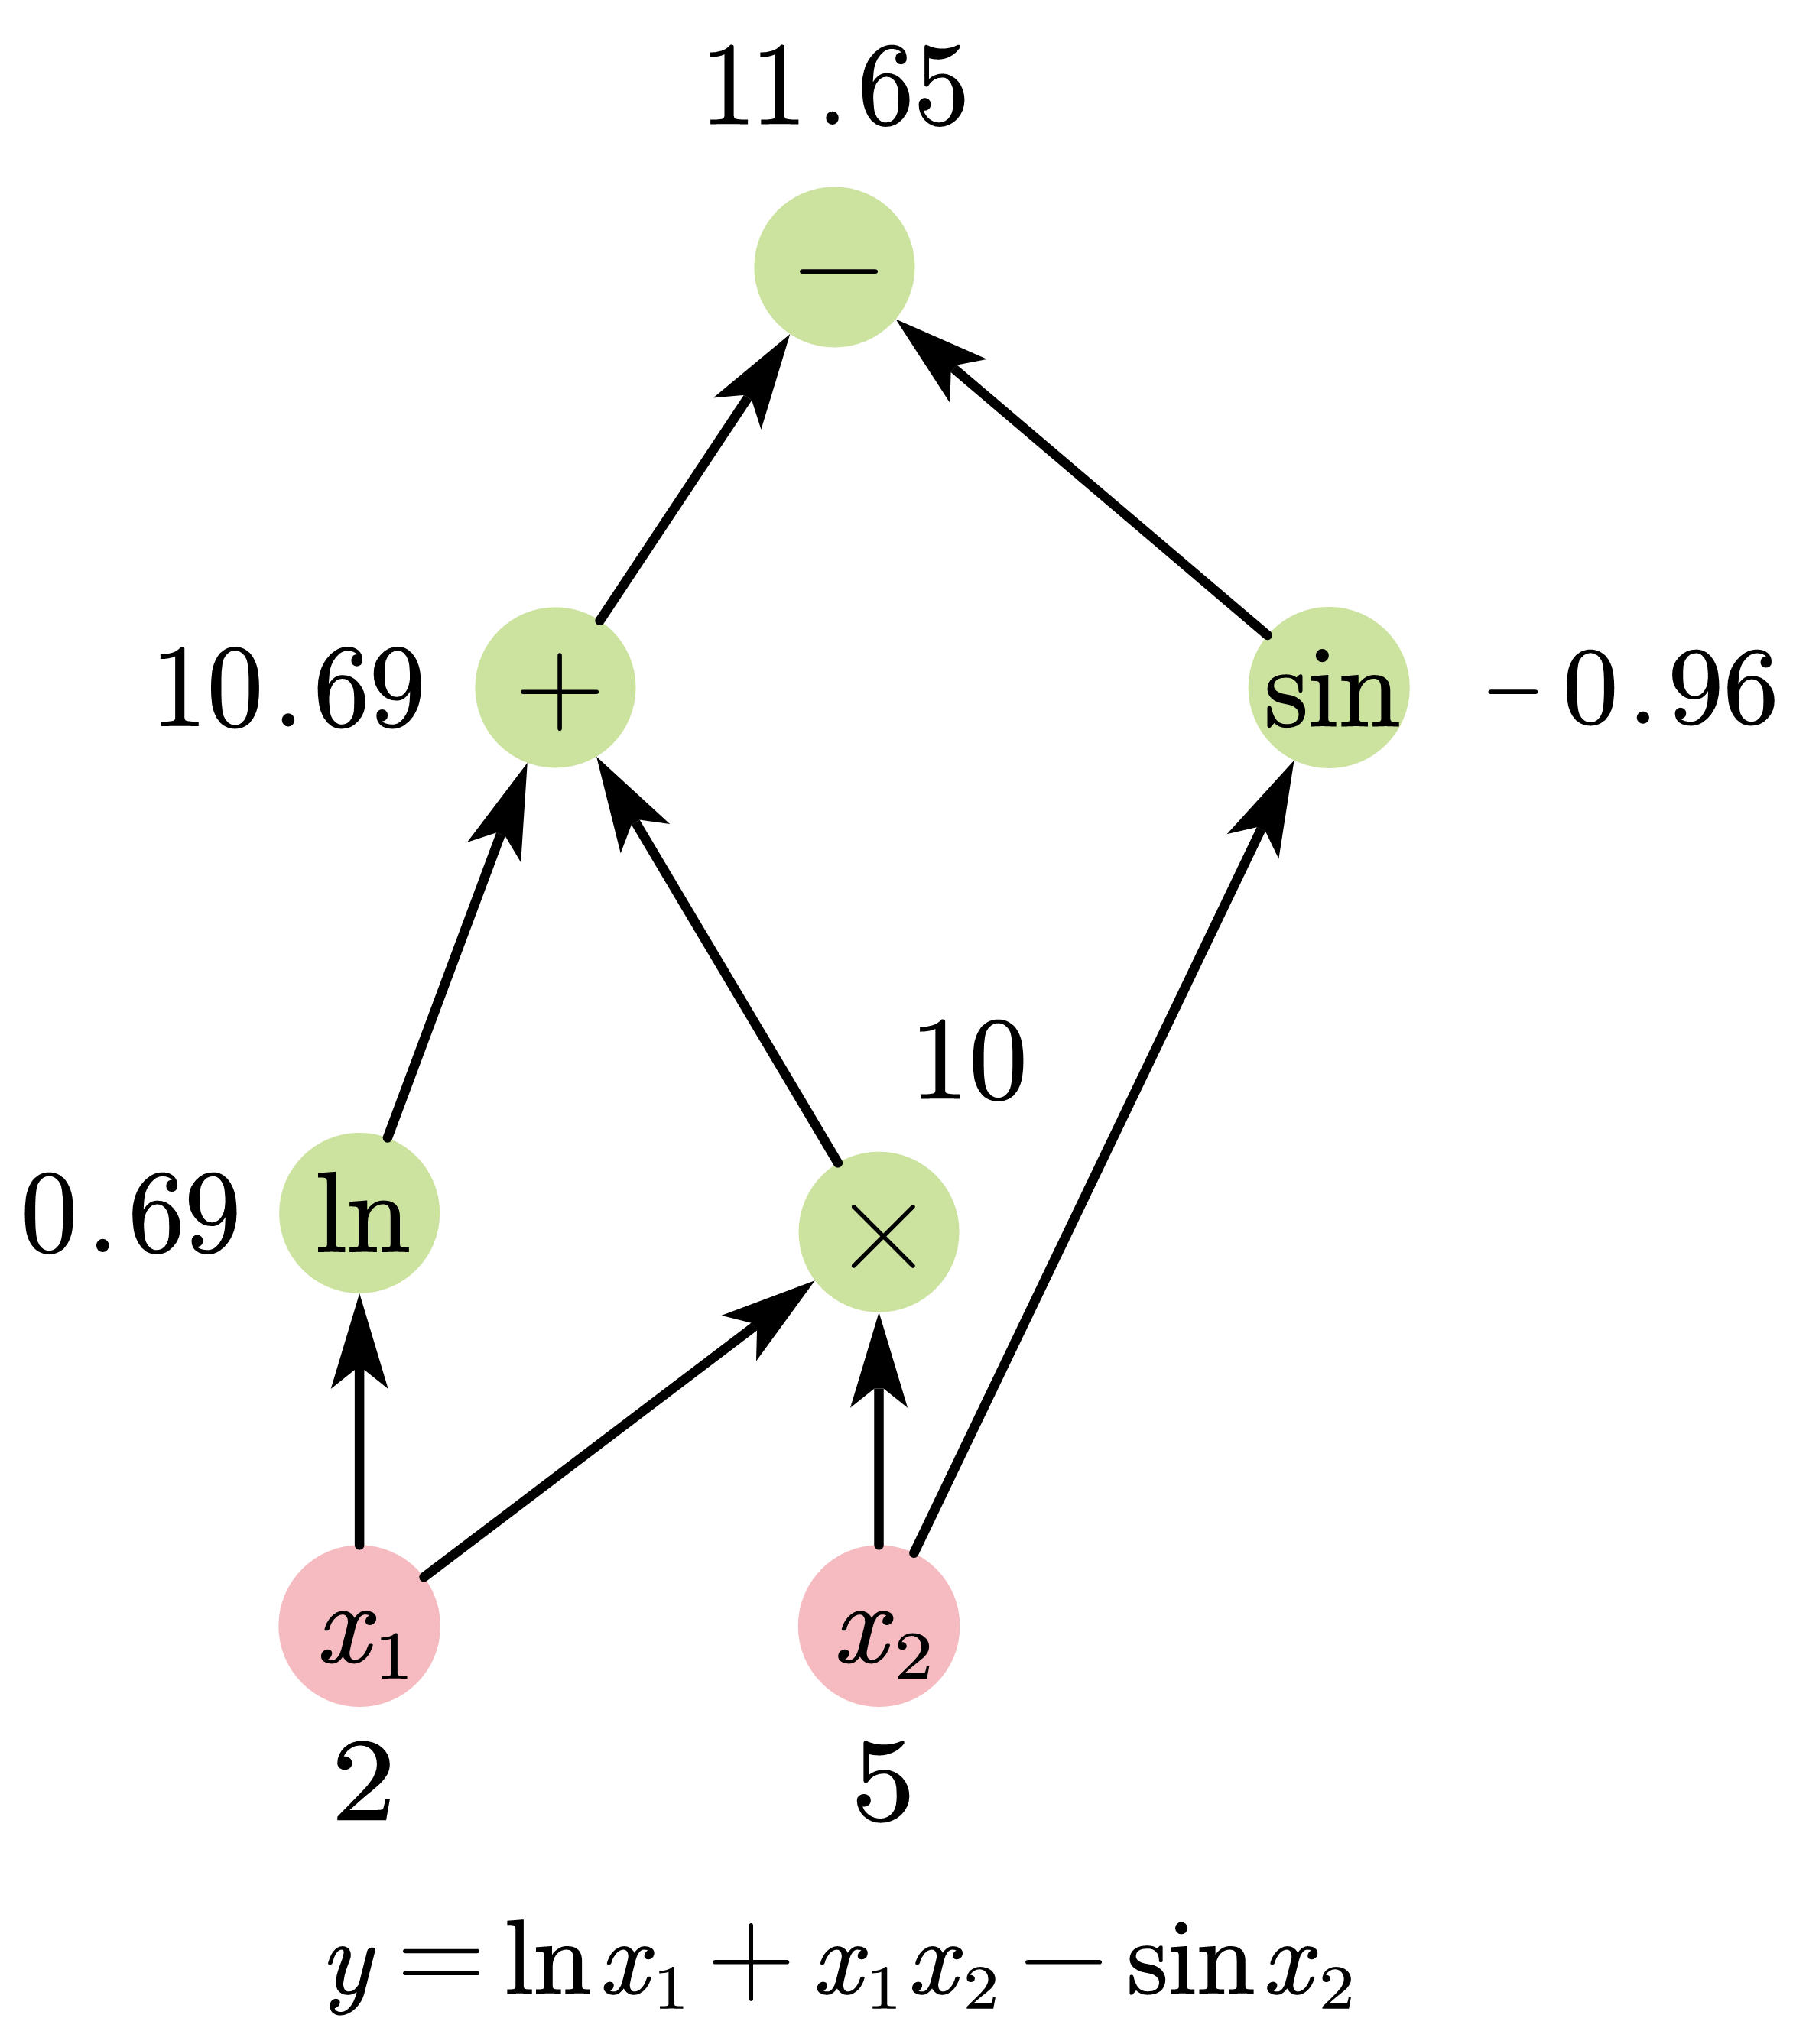
\includegraphics[width=7cm]{figure/ComputingGraph.png}
\end{center}
图有两个基本要素:变量与运算。通过这个图来计算微分,具体计算有两种模式:前向与反向模式。前者是指从变量出发,一次计算中间值与微分;后者是先前向计算函数值,再反向计算微分。反向模式在机器学习中比较常用。

变量可以是张量,包括矩阵、向量在内。图中每个节点只需要存储函数值与微分值。
\subsubsection{反向模式}
计算过程如下:
\begin{center}
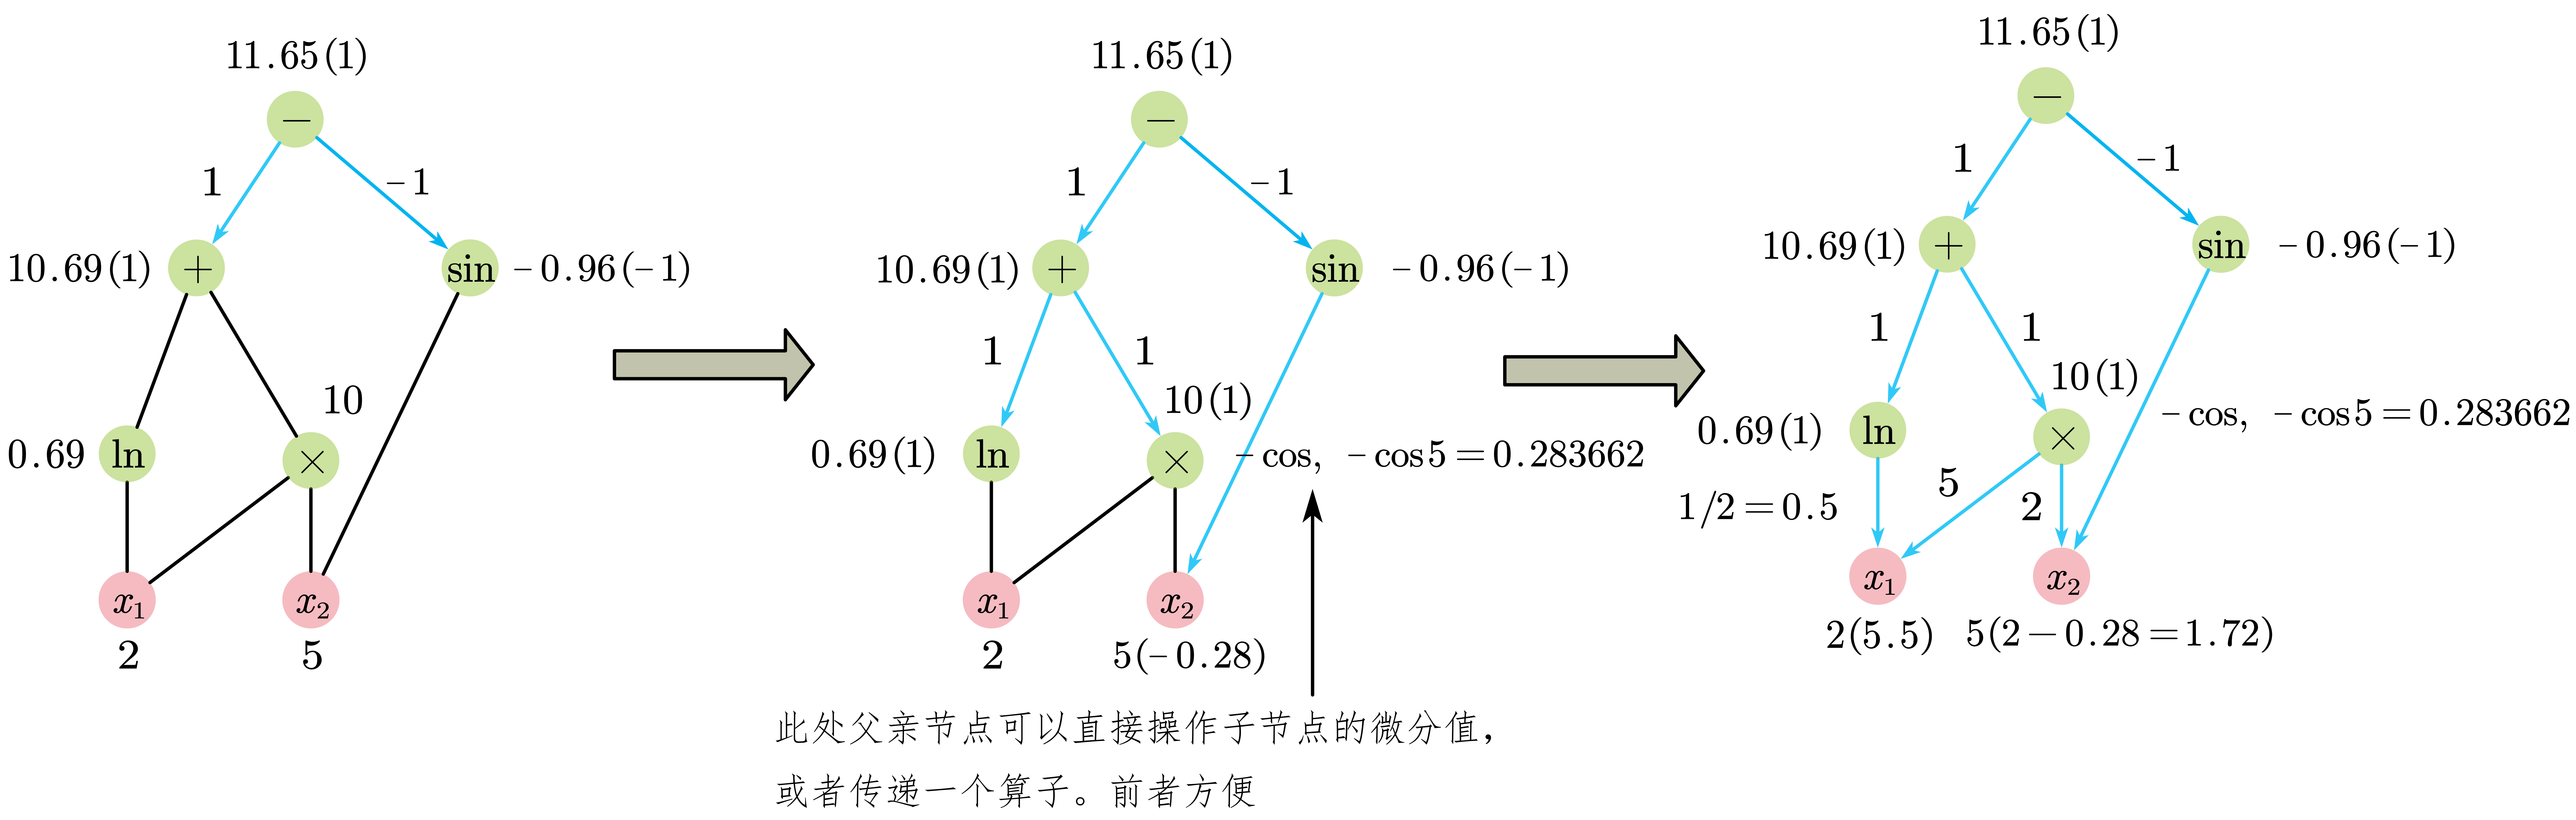
\includegraphics[width=\linewidth]{figure/ReverseMode.png}
\end{center}
节点存储值与微分,父亲节点可以操作子节点的微分值。
\subsubsection{一元运算}

\subsubsection{二元运算}

\subsubsection{矩阵运算}
\paragraph*{转置}转置是很特殊的操作,它本身是一元运算,但它会改变变量的数据结构,所以不能等同于计算图中一个变量输出多条边。
\section{矩阵微分应用实例}
\subsection{神经网络的BP传播}
以下给出一个二次网络的例子:
$$\bm{y}_k=f(\bm{x}_{k-1})=f(g_{k-1}(\by_{k-1}))=f\left(U_{k-1}\by_{k-1}^{\odot 2}+V_{k-1}\by_{k-1}+\bm{b}_{k-1}\right)$$
模型参数是$U_k,V_k,\bm{b}_k$。$\odot$表示Element-wise操作,比如$\bx\odot\by=\diag(\bx)\by$,$\diag(\cdot)$函数假如参数是列向量,则结果是对角矩阵,如果参数是矩阵,结果是对角线构成的列向量。那么$\by_{k-1}^{\odot 2}$表示Element-wise的多项式。注意,这里我们是用的$\by_k$,而不是题目中的$\bx_k$,这是为了方便。$\by_k$为第$k$层在损失函数作用之后的输出,不妨设整个网络输入为第0层,输入为$\bm{y}_0$,最终输出是第$M$层,输出$y_{M}$。于是整个模型表示为

\begin{center}
\begin{tikzcd}[column sep=small]
	\bm{y}_0\arrow[r,"g_0"]& \bm{x}_0 \arrow[r,"f"] & \bm{y}_1\arrow[r,"g_1"]&\bm{x}_1\arrow[r,"f"]&\cdots\arrow[r,"f"]&\bm{y}_{M-1}\arrow[r,"g_{M-1}"]&x_{M-1}\arrow[r,"f"]&y_M\arrow[r,"\mathcal{L}"]&L
\end{tikzcd}
\end{center}
$\mathcal{L}$为损失函数,$L$为最终的损失函数值。可以看出$\bx$的下标数量比$\by$少1。

假如只有一个隐藏层,那么应该是
\begin{center}
	\begin{tikzcd}[column sep=small]
		\bm{y}_0\arrow[r,"g_0"]& \bx_0 \arrow[r,"f"] & \by_1\arrow[r,"g_1"]&x_1\arrow[r,"f"]&y_2\arrow[r,"\mathcal{L}"]&L
	\end{tikzcd}
\end{center}
此时$U_1,V_1$是矩阵,而$U_2,V_2$是行向量,$y_1,x_1$是列向量,$y_2,x_2$是标量。

另外取
\begin{empheq}{align*}
f(x)&=\frac{1}{1+e^{-x}}\\
f'(x)&=f(x)(1-f(x))\\
\mathcal{L}(y_M;y)&=-\left(y\ln y_M+(1-y)\ln(1-y_M)\right)\\
\mathcal{L}'(y_M)&=\frac{1-y}{1-y_M}-\frac{y}{y_M}
\end{empheq}

由于是二分类问题,所以上面取的是损失函数是Binary Cross-Entropy函数。

我们的目标是计算损失对参数的导数,即$\pdv{L}{U_k},\pdv{L}{V_k},\pdv{L}{\bm{b}_k}$
。然后利用梯度下降法来更新:
\begin{empheq}{align}
U_k^{(t+1)}&=U_k^{(t)}-\eta\E\left(\pdv{L}{U_k^{(t)}}\right)\\
V_k^{(t+1)}&=V_k^{(t)}-\eta\E\left(\pdv{L}{V_k^{(t)}}\right)\\
\bm{b}_k^{(t+1)}&=\bm{b}_k^{(t)}-\eta\E\left(\pdv{L}{\bm{b}_k^{(t)}}\right)
\end{empheq}
其中$\E(\cdot)$为期望,可以用在样本点处的导数的均值来代替。

利用全微分,有
\begin{empheq}{align}
\dif \bm{x}_k=&(\dif U_{k}) \by_{k}^{\odot 2}+2U_{k}\diag(\by_{k})\dif \by_{k}+(\dif V_{k}) \bm{y}_{k}+V_{k}\dif \by_{k}+\dif \bm{b}_k\nonumber\\
=&(\dif U_{k}) \by_{k}^{\odot 2}+(2U_{k}\diag(\by_{k})+V_{k})\dif \by_{k} +(\dif V_{k}) \bm{y}_{k}+\dif\bm{b}_{k}\\
\dif \bx_0=&(\dif U_0) \by_{0}^{\odot 2}+(\dif V_0) \bm{y}_{0}+\dif \bm{b}_0\label{total_dif_1}\\
\dif \bm{y}_k=&f'(\bx_{k-1})\odot\dif \bx_{k-1}\label{total_dif_2}\\
\dif L=&\mathcal{L}'(y_M)\dif y_M\label{total_dif_3}
\end{empheq}
强调这里的求导是对于单个样本而言的。

从全微分中得到偏微分时,可以忽略掉不相关的项,比如
$$\dif L=\mathcal{L}'(y_{M})f'(x_{M-1})(dU_{M-1})\by_{M-1}^{\odot 2}+C$$
那么
$$\frac{\partial L}{\partial U_M}=\mathcal{L}'(y_M)f'(x_{M-1})(\by_{M-1}^{\odot 2})^T$$
这里使用了两个技巧。第一,如果$\frac{\dif L}{\dif A}=B$,那么$\dif L=\sum_{i,j}(\dif A\odot B)=\trace(B^T\dif A)=\trace((\dif A)B^T)$,反之亦然。第二,$\bx^T\by=\trace(\bx^T\by)=\trace(\bx\by^T)$。

类似地有:
\begin{empheq}{align}
\pdv{L}{V_M}&=\mathcal{L}'(y_M)f'(x_{M-1})(\by_{M-1})^T\\
\pdv{L}{\bm{b}_M}&=\mathcal{L}'(y_M)f'(x_{M-1})
\end{empheq}

现在考虑$\dif\bx$的展开式中的$\dif \by_{k-1}$项,它展开后,可以得到$\dif U_{k-1},\dif V_{k-1},\dif \by_{k-2}$,前两个项可以用于求偏导。此时
$$\dif L=\mathcal{L}'(y_M)f'(x_{M-1})(2U_{M-1}\diag(\by_{M-1})+V_{M-1})\dif \by_{k-1}+C$$
所以要求$V_{k-1}$的偏导数,就要展开$\dif \by_{k-1}$项。不妨假设$\dif \by_{k}$项的系数矩阵是$A_{k}$,那么
\begin{empheq}{align}
A_M&=\mathcal{L}'(y_M)\label{init0}\\
\dif L&=\mathcal{L}'(y_M)\dif y_M\\
&=A_{k}\dif \by_{k}+C\\
&=A_{k}\diag(f'(\bx_{k-1}))\dif \bx_{k-1}+C
\end{empheq}

那么可以得到
\begin{empheq}{align}
\pdv{L}{\bm{b}_{k-1}}&=\diag(f'(\bx_{k-1}))A_{k}^T\label{rec1}\\
\frac{\partial L}{\partial U_{k-1}}&=\diag(f'(\bx_{k-1}))A_{k}^T(\by_{k-1}^{\odot 2})^T=\pdv{L}{\bm{b}_{k-1}}(\by_{k-1}^{\odot 2})^T\label{rec2}\\
\pdv{L}{V_{k-1}}&=\diag(f'(\bx_{k-1}))A_{k}^T(\by_{k-1})^T=\pdv{L}{\bm{b}_{k-1}}(\by_{k-1})^T\label{rec3}\\
A_{k-1}&= A_{k}\diag(f'(\bx_{k-1}))(2U_{k-1}\diag(\by_{k-1})+V_{k-1})\label{rec4}
\end{empheq}

注意$A_0$其实是没用的,可以从\cref{total_dif_1}看出来,$\dif x_0$的展开式中没有$\dif \bm{y}_0$。

至此,已经给出了反向传播的全部递推式。即由\cref{init0,rec1,rec2,rec3,rec4}可以进行反向传播。在实现的时候,可以把$U_k,V_k,\bm{b}_k,A_k,\bx_{k},\by_k$存储在向量中,然后按下标访问。
\chapter{矩阵积分}

\section{多变量高斯分布积分}
\subsection{密度函数}
$$f(\bx)=(2\pi)^{-\frac{n}{2}}|\Sigma|^{-\frac{1}{2}}e^{-\frac{1}{2}(\bx-\mu)^T\Sigma^{-1}(\bx-\mu)}$$
\subsection{由联合分布诱导条件分布}
假设两个高斯向量$\bx,\by$服从联合高斯分布。记
\[
\bmu=\begin{bmatrix}
\bmu_{\bx}\\
\bmu_{\by}
\end{bmatrix},\Sigma=\begin{bmatrix}
\Sigma_{\bx}&\Sigma_{\bx\by}\\
\Sigma_{\by\bx}&\Sigma_{\by}
\end{bmatrix}
\]

\chapter{张量代数}
张量代数在这些地方有出现过:
\begin{enumerate}
\item 理论物理学。
\item 线性代数中的张量积。
\item 范畴论中的共变与反变函子。
\end{enumerate}
从上到下,抽象程序依次提升。这里取中间的一层,即作为多线性代数的张量。

\section{理解张量}
\subsection{理解坐标变换}
\subsubsection{坐标变换与基变换}
坐标变换与基变换,并不完全是一回事。比如用$x_i$表示笛卡尔坐标系的坐标,$\bm{e}^i$表示笛卡尔坐标系的基。给定坐标变换
\begin{empheq}{align*}
x^1&=x_1+x_2\\
x^2&=x_1-x_2-5
\end{empheq}
这是一个平移变换。我们可能设想对应的基变换是直接把坐标换掉:
\begin{empheq}{align*}
	\bm{e}_1&=\bm{e}^1+\bm{e}^2\\
	\bm{e}_2&=\bm{e}^1-\bm{e}^2-5
\end{empheq}
但这是不对的,注意下面一行,左边是向量,而5是常数,相减其实没有定义。而且由于坐标变换中,涉及常数,所以并不能直接用二维笛卡尔基来表示基变换。

\subsubsection{坐标变换的方向}
坐标变换是一个笼统的概念,从函数的角度考虑,一个映射,有定义域与值域的区别,因此在具体的量中进行坐标变换时,也会存在方向的问题。即坐标可以以其它量为参数(是值域),或者是其它量的参数(定义域)。

考虑速度向量,坐标系是$(x^1,x^2,x^3)$,它是时间$t$的函数,则速度向量为
$$(\xi^1,\xi^2,\xi^3)=\left(\odv{x^1}{t},\odv{x^2}{t},\odv{x^3}{t}\right)$$

现在我们有一个新的坐标系$(z^1,z^2,z^3)$,此时使用坐标变换$x^i\rightarrow z^i$,即$x$是$z$的函数,给定$x$,可以求得新坐标$z$。在新坐标系下,速度向量为
\begin{equation}\label{velocity-vector}
\eta^i=\odv{z^i}{t}=\xi^j \pdv{z^i}{x^j}
\end{equation}

新坐标$\bz$在上边,因此速率向量为$(1,0)$张量。

另一方面,又考虑梯度向量。原坐标系也是$(x^1,x^2,x^3)$,函数为$f(x^1,x^2,x^3)$,梯度为
$$\nabla f(x^1,x^2,x^3)=\left(\pdv{f}{x^1},\pdv{f}{x^2},\pdv{f}{x^3}\right)=(\xi^1,\xi^2,\xi^3)$$。现在有一个新坐标系$(z^1,z^2,z^3)$,此时的坐标变换应该为$z^i\rightarrow x^i$,即把$x^i$用$\bz$表示出来,这样才能算出$f$,于是现在新坐标系下
$$\eta_i=\pdv{f}{z^i}=\xi^j\pdv{x^j}{z^i}$$

注意$\eta_i$的下标,对应于$\partial z^i$在下边,因此梯度为$(0,1)$张量。

对比以上两个例子,可以看出,虽然都是坐标变换,但其实方向恰好相反,这种方向上的区别就是协变与共变的区别。然而实际上都是链式法则。

\subsubsection{为什么使用张量}
参考系在物理学中的地位非常重要,同样的物理量,在不同的参考系下有不同的表示。常规情况下,在一个坐标系下进行计算的结果,在新坐标系下,需要重新计算一遍:
\begin{center}
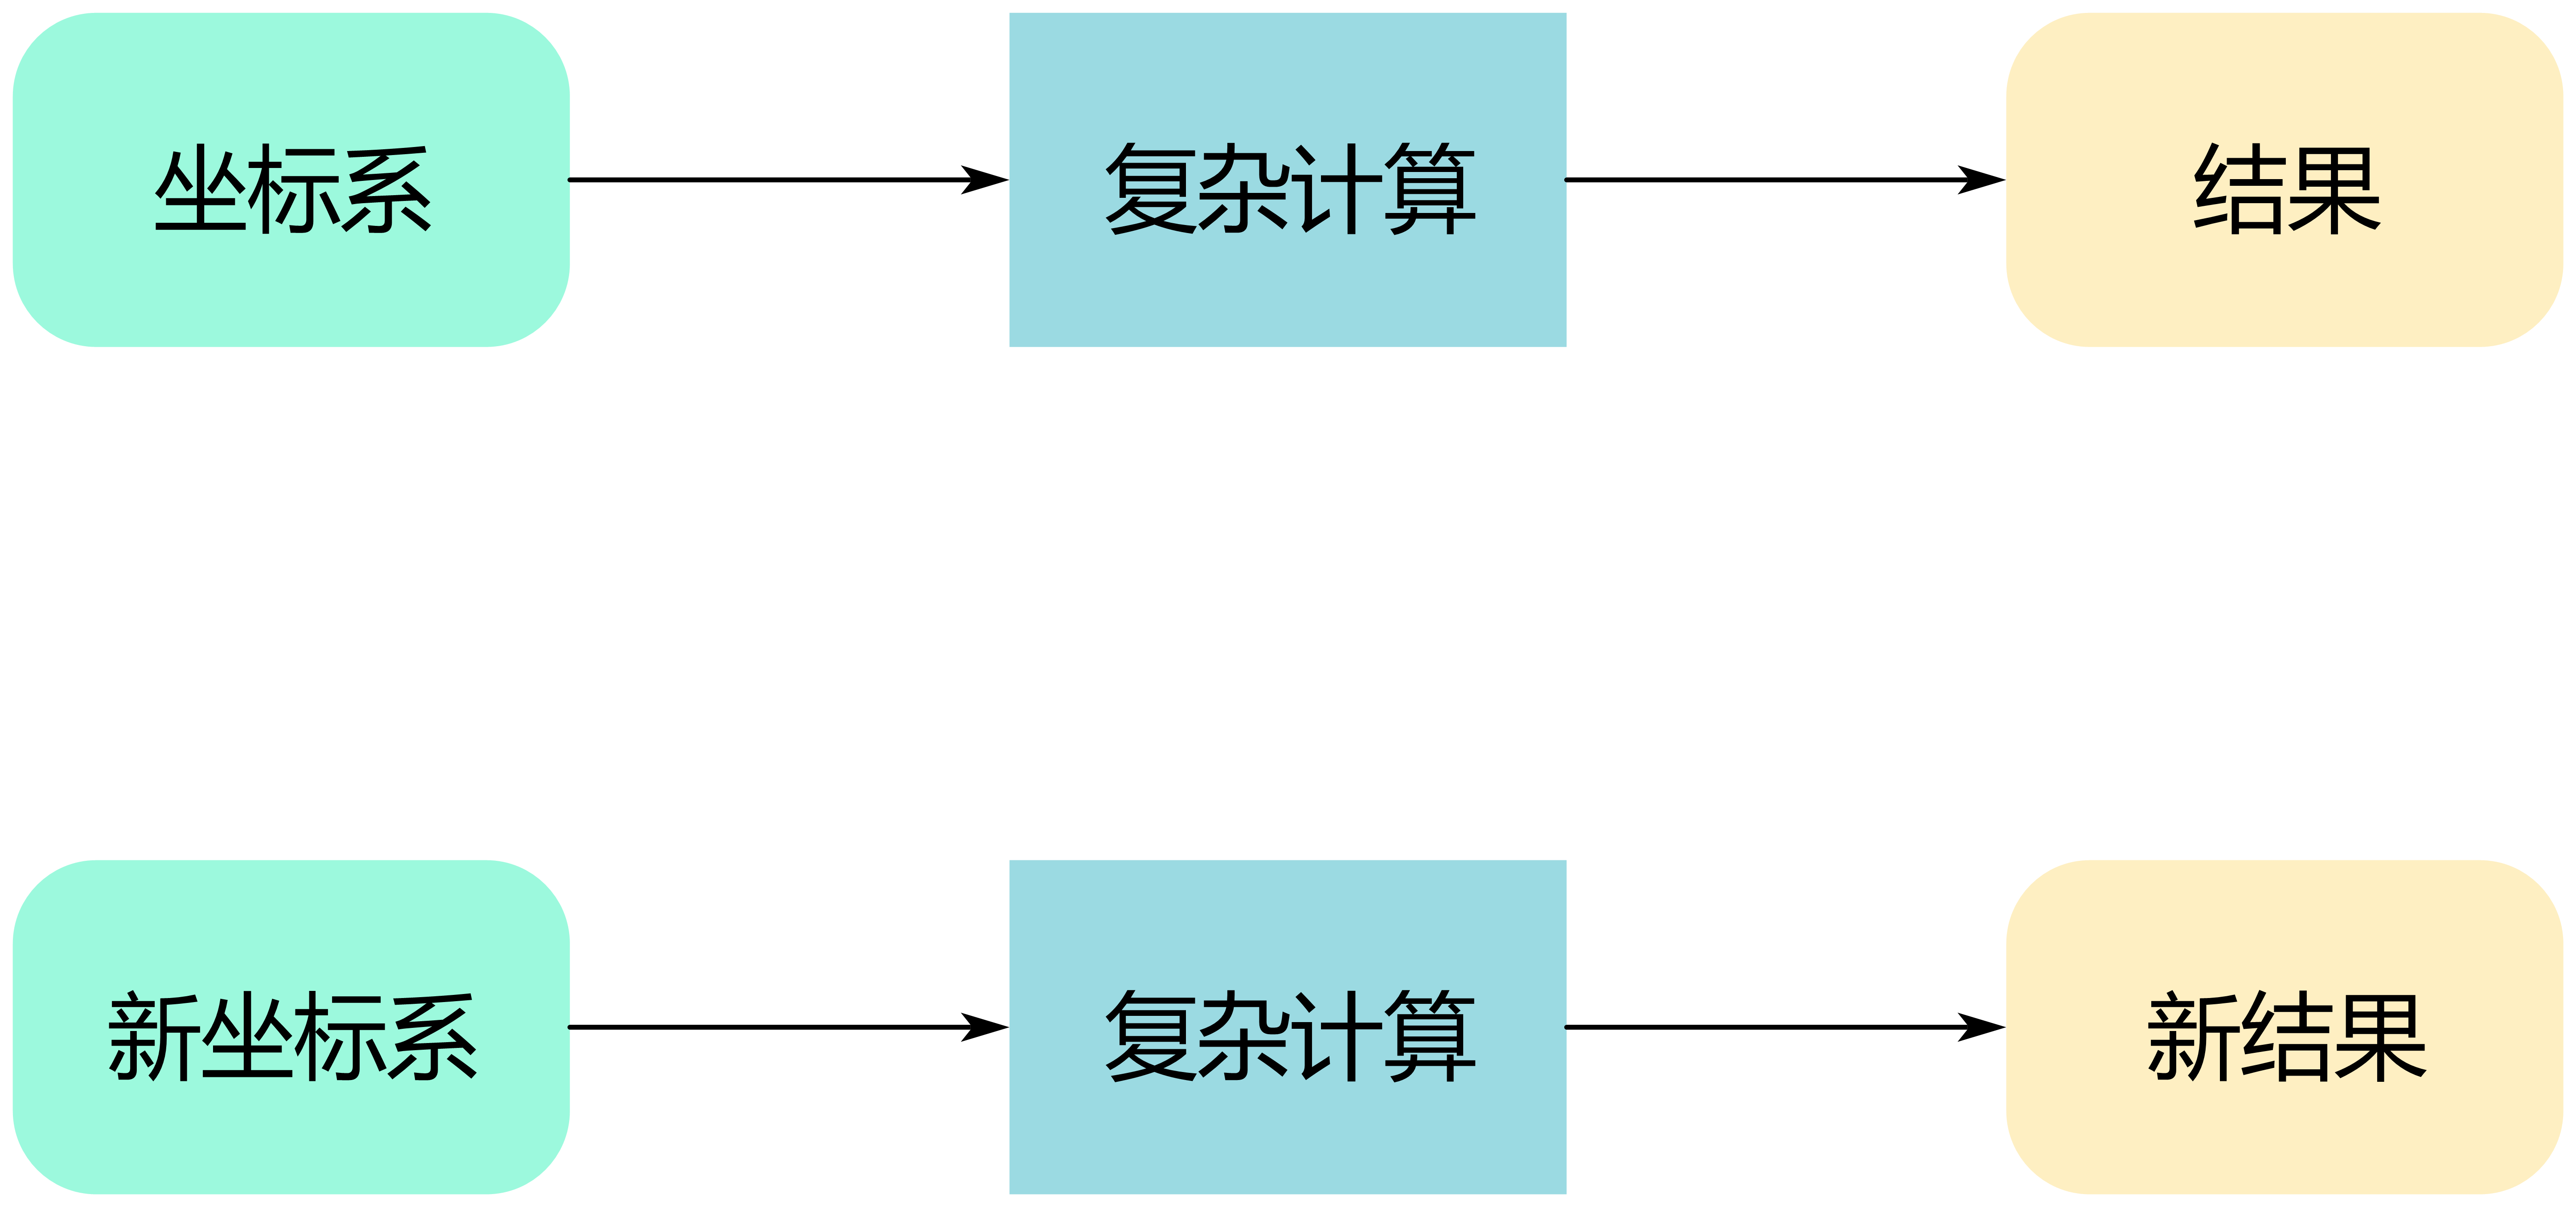
\includegraphics[width=8cm]{figure/NoTensor.png}
\end{center}
这样是非常繁琐的,而且不同的坐标系是无限多的。

现在引入张量,张量就是在坐标变换下不变的量。张量本身在不同的坐标系下是不变的,但张量在不同坐标系下的表示却是不同的。有了张量,我们就只需要在一个坐标系下进行计算,得出结果,然后找出坐标变换,对结果也进行一下坐标变换,就得到了在新坐标系下的结果,不需要重行进行计算:
\begin{center}
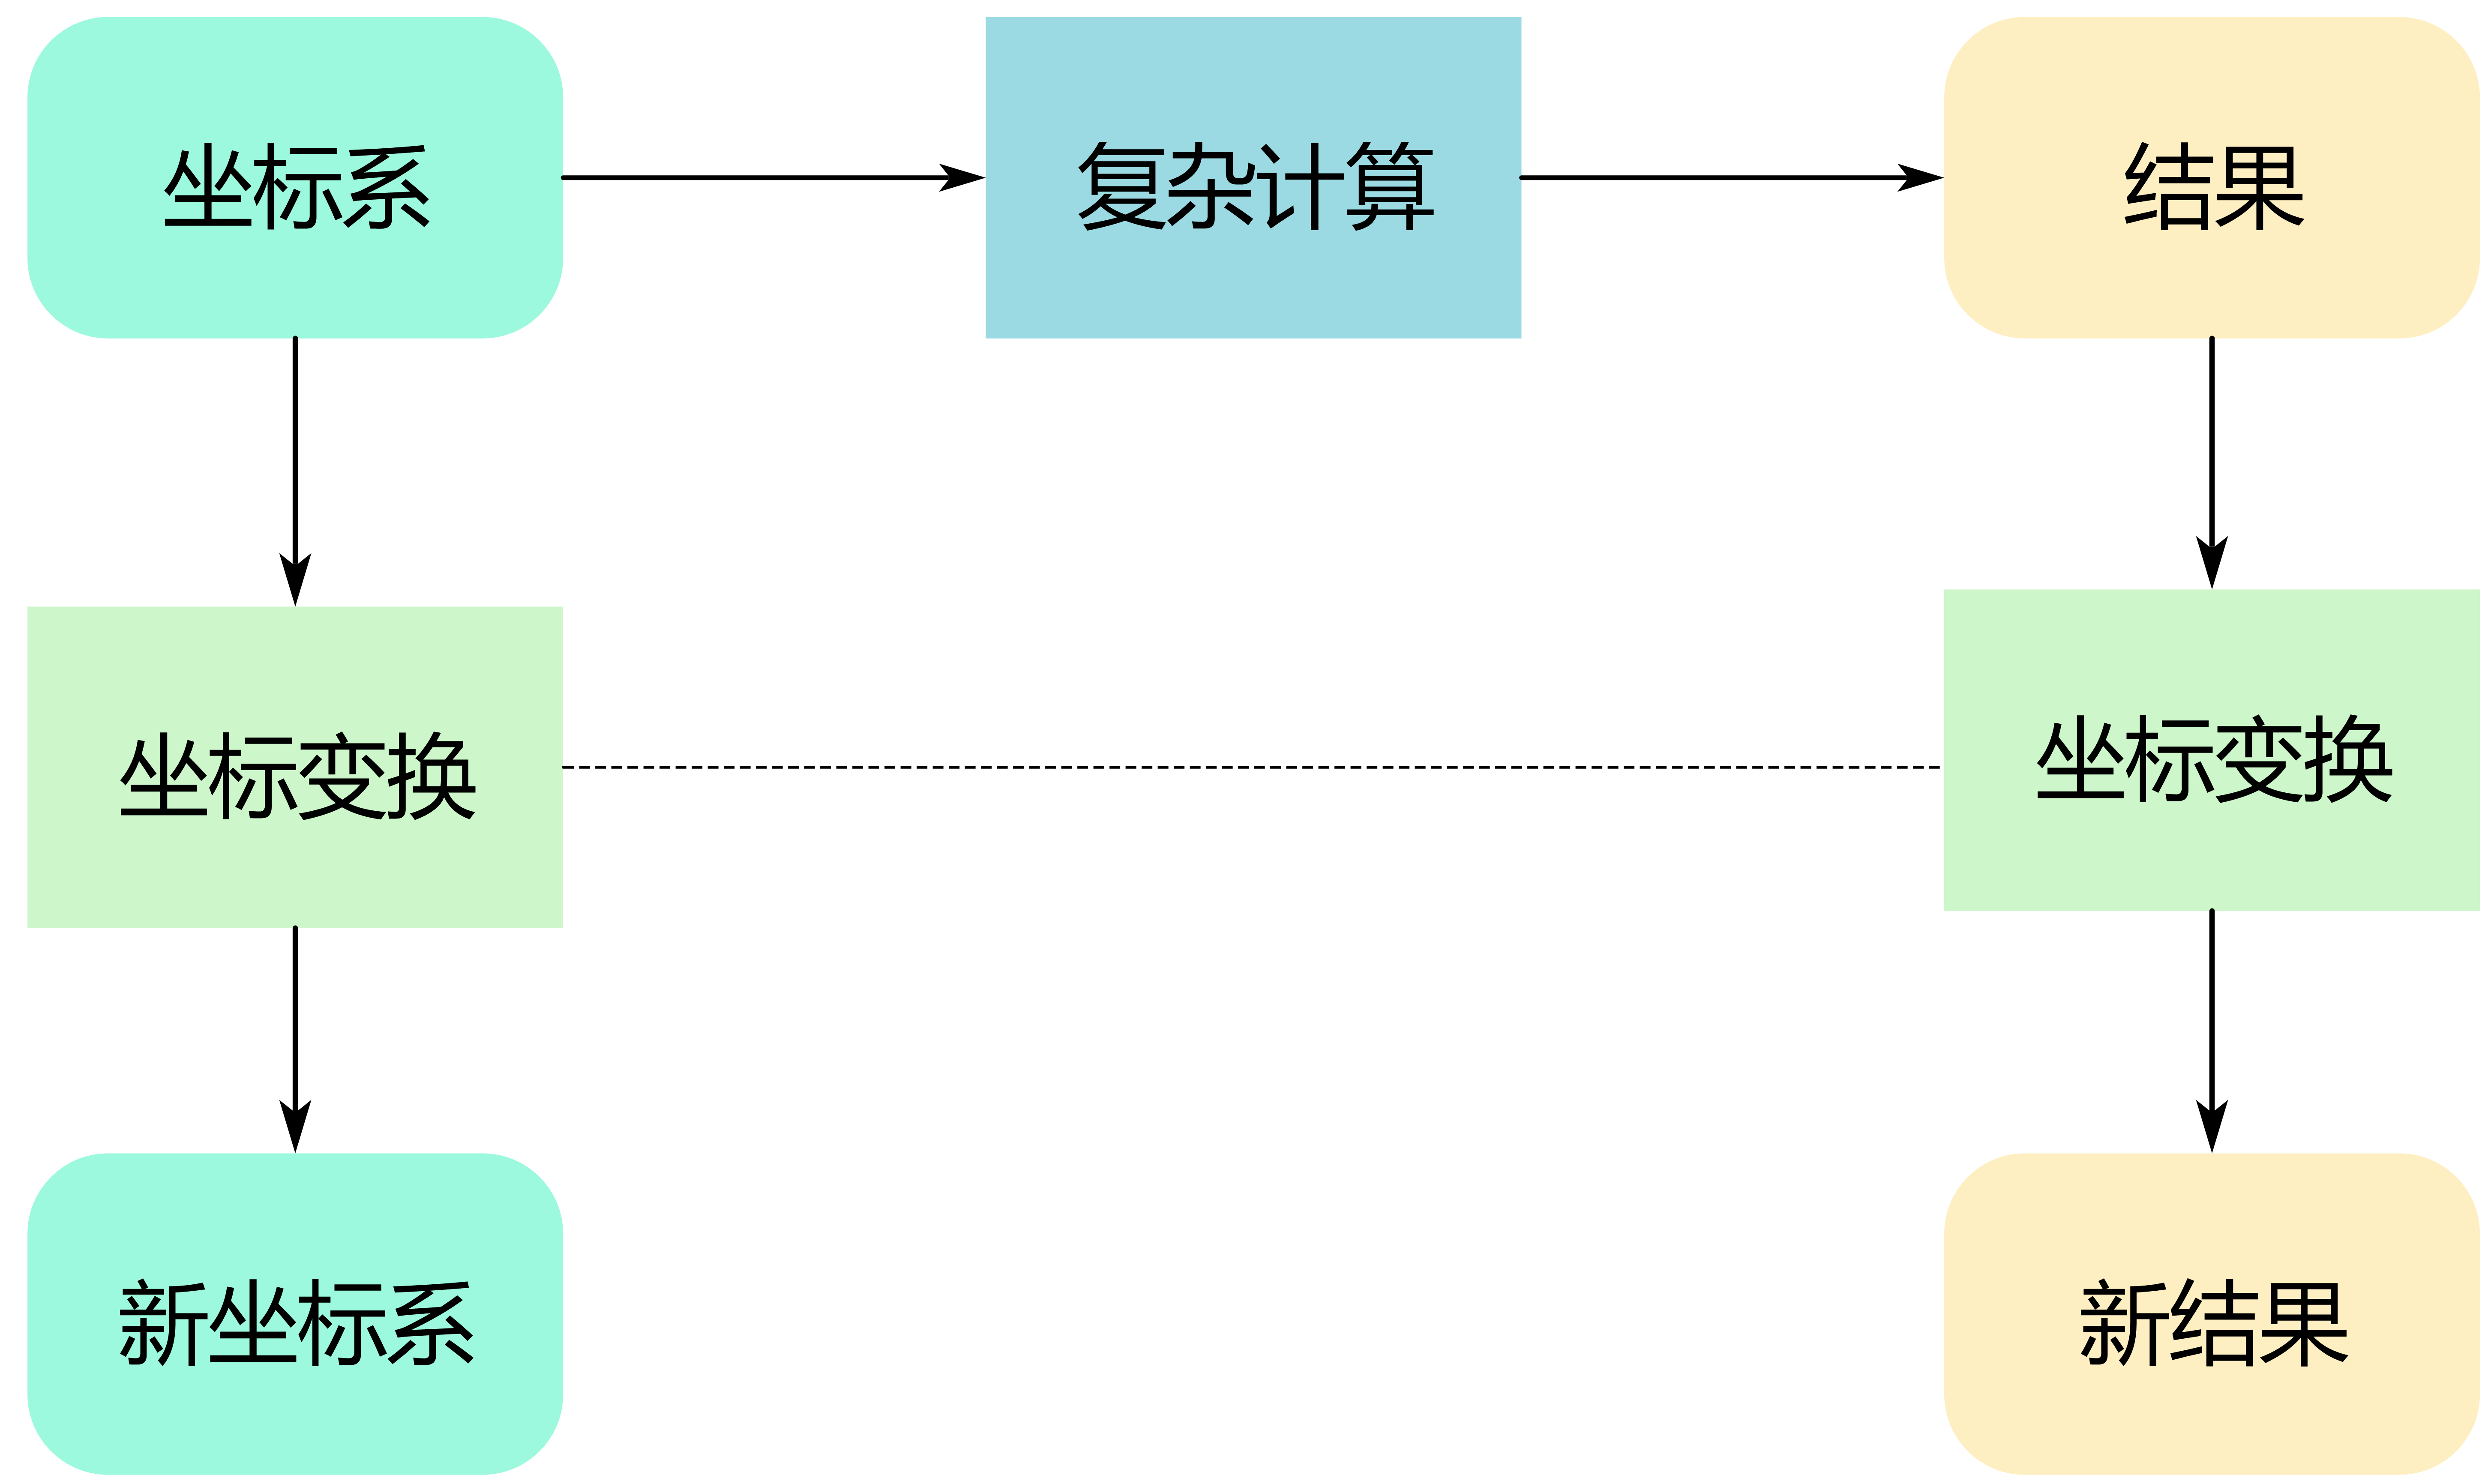
\includegraphics[width=8cm]{figure/WithTensor.png}
\end{center}
\subsection{协变与逆变(或共变与反变)}
在线性代数中,记$E$的列$\{\bm{e}_1,\cdots,\bm{e}_n\}$为某个坐标系下的基,则给定坐标变换
$$E'=ET$$
$T$称为从基$\{\bm{e}_1,\cdots,\bm{e}_n\}$到基$\{\bm{e}_1',\cdots,\bm{e}_n'\}$的过渡矩阵。

假设在某个坐标系$E$下,某个欧几里得空间中的向量表示为$\bx$,那么在基变换$T$下有$E'=ET$,由于张量是不变的,所以
\[
\begin{aligned}
E'\bx'&=E\bx\\
ET\bx'&=E\bx\\
x'&=T^{-1}x
\end{aligned}
\]

注意到坐标变换式与基变换式恰好相反,所以欧几里得空间中的张量是一次反变张量。

我们说的反变与共变张量是指张量在坐标变换下的性质。似乎与反变分量、共变分量并不完全一样,说反变、共变分量时,一定是针对基与对偶基而言的,而基与对偶基(reciporical basis)之间需要满足某种关系,并不能随意选取。关于反变与共变分量需要记住:
\begin{center}
\textbf{张量在共变基下的分量叫反变分量。}\\
\textbf{张量在反变基下的分量叫共变分量。}
\end{center}
这里可以看出,爱因斯坦求和是对上指标与下指标求和。

$(p,q)$型张量称为$p$次反变($p$个反变基)、$q$次共变($q$个共变基)张量,表示为$T^p_q(V)$,可见上标是反变,下标是共变。


\subsection{张量的例子}

\section{Einstein记号与张量乘法}
\subsection{多维数组的Einstein记号}
以下用$A_{ij}$来表示一个二维数组。使用Einstein记号可以很方便地表示多维数组的乘法和一些运算:
\subsubsection{矩阵运算}
\begin{empheq}{align}
AB&=Y_{ij}=A_{ik}B_{kj} \mtag{矩阵乘法}\\
ABC&=Y_{ij}=A_{ik}B_{kl}C_{lj}\\
ABCD&=Y_{ij}=A_{ik}B_{kl}C_{lm}D_{mj}\\
A^TA&=Y_{ij}=A_{ki}A_{kj}\\
XA^TAX^T&=Y_{ij}=X_{ik}A_{lk}A_{lm}X_{jm}\\
\bx^TA\by&=L=x_iA_{ij}y_j
\end{empheq}
以下用$[\underline{\bx^T}_m]$表示把一个行向量沿行方向复制多份,构成矩阵。$A\odot [\underline{\bx^T}_m]$就是把矩阵$A$的每一行按元素乘以$\bx$。
\begin{empheq}{align}
A\odot [\underline{\bx^T}_m] &=Y_{ij}=A_{ij}x_j
\end{empheq}
\begin{empheq}{align}
\trace(A)&=L=A_{ii}\\
\trace(AB)&=L=A_{ik}B_{ki}\\
\trace(XAX^T)&=L=X_{ik}A_{kl}X_{li}\\
\trace(XA^TAX^T)&=L=X_{ik}A_{lk}A_{lm}X_{im}
\end{empheq}
\begin{empheq}{align}
\diag(A)&=\bx_{i}=A_{ii}\\
\diag(AB)&=\bx_{i}=A_{ij}B_{ji}
\end{empheq}
\section{张量的定义}
\subsection{$(p,q)$型张量}
\begin{definition}[$(p,q)$型张量]{}
称在坐标系$(x^1,\cdots,x^n)$下给出的数组$T^{i_1\cdots i_p}_{j_1\cdots j_q}$为$p+q$阶的$(p,q)$型张量是指它按如下方式在依赖于坐标系:

$$T^{i_1\cdots i_p}_{j_1\cdots j_q}=\sum_{k,l}{T'}^{k_1\cdots k_p}_{l_1\cdots l_q}\pdv{x^{i_1}}{z^{k_1}}\cdots\pdv{x^{i_p}}{z^{k_p}}\pdv{z^{l_1}}{x^{j_1}}\cdots\pdv{z^{l_q}}{x^{j_1}}$$
\end{definition}
以之前的速度向量\eqref{velocity-vector}为例,在$\bz$坐标系下,其表示式中$\partial z^i$在上边,因此就是$(1,0)$型张量。

\part{分析学}
\chapter{复分析}
\section{复数}
\subsection{复数的运算法则}
\begin{empheq}{align}
e^{ix}&=\cos x+i\sin x\\
\left|re^{ix}\right|&=|r|\\
|a+bi|&=\sqrt{a^2+b^2}\\
\left|r_1e^{ix}+r_2e^{-ix}\right|&=\sqrt{(r_1+r_2)^2-4r_1r_2\sin^2 x}\label{complex-sum-abs}
\end{empheq}
\chapter{实分析}

\section{实数集的完备性}

\section{收敛与极限}
\subsection{极限的定理}
\subsubsection{洛必达法则}

\subsubsection{Stoltz定理}
\begin{theorem}[Stoltz定理]
假设$\{x_n\}_{n=1}^\infty,\{y_n\}_n=1^\infty$是2个序列,满足
\begin{enumerate}
\item $\{y_n\}_{n=1}^\infty$单调增加,且发散。
\item $\lim\limits_{n\rightarrow\infty}\frac{x_n-x_{n-1}}{y_n-y_{n-1}}=C$为一常数。
\end{enumerate}
那么
$$\lim\limits_{n\rightarrow\infty}\frac{x_n}{y_n}=C$$

实际上这个定理相当于洛必达法则。
\end{theorem}
\begin{lemma}[等差数列均值的极限]\label{Stoltz-l1}
如果
$$\lim_{n\rightarrow\infty} (a_{n+1}-a_n)=a$$
那么有
$$\lim_{n\rightarrow\infty}\frac{a_n}{n}=a$$

要得到这个公式,在Stoltz定理中取$y_n=n$即可。
\end{lemma}
\subsection{极限计算的例子}
\subsubsection{与指数函数相关}
\begin{example}
	\begin{empheq}{equation}
		\lim_{x\rightarrow \infty}x\left(1-e^{-\frac{a}{x^2}}\right),a>0
	\end{empheq}
\end{example}
\begin{solution}
	右边$\rightarrow$0,左边$\rightarrow \infty$,乘积是不定的。但指数函数收敛快,所以右边趋近0快,有可能收敛。
\begin{empheq}{align*}
\text{原式}&\xRightarrow{u=1/x}\\
\lim_{u\rightarrow 0}&=\frac{1-e^{-au^2}}{u}\\
	&=\frac{e^{au^2}-1}{ue^{au^2}}\\
	&=0
\end{empheq}
\end{solution}

\chapter{微积分}\label{diff-int}
\section{一元微分}
\subsection{导数公式}
\paragraph*{实函数}
\begin{empheq}{align*}
\odv{f(x)}{x}&=f'(x)=\lim_{h\rightarrow 0}\frac{f(x+h)-f(x)}{h}\\
\frac{\dif^n f(ax)}{\dif x^n}&=a^nf^{(n)}(u)\big|_{u=ax}\\
\frac{\dif f(x)}{\dif x}&=\frac{\dif \ln f(x)}{\dif x}f(x)\\
\odv{fg}{x}&=f'g+fg'\\
\odv[order=2]{fg}{x}&=f''g+2f'g'+fg''\\
\odv[order=n]{fg}{x}&=\sum_{k=0}^{n} \binom{n}{k}f^{(k)}g^{(n-k)} 
\end{empheq}

\paragraph*{复函数}
记$z=x+iy,f(z)=u(x,y)+iv(x,y)$,则假如$f$满足柯西——黎曼方程:
\begin{empheq}{align}
\pdv{u}{x}&=\pdv{v}{y}\\
\pdv{u}{y}&=-\pdv{v}{x}
\end{empheq}
那么有复函数的导数:
\begin{empheq}{align}
f'(z)&=\pdv{u}{x}+i\pdv{v}{x}\\
\odv{f(x)e^{ig(x)}}{x}&=f'e^{ig}+fe^{ig}ig'=e^{ig}(f'+ifg')
\end{empheq}

此外常见初等函数$(z^n,\ln z,\sin z,\sinh z,\cdots)$的复导数与实导数形式相同,如$\odv{z^2}{z}=2z$。
\section{多元微分与向量分析}
\subsection{Jacobi矩阵}
多元函数的一阶微分.

\[
J\left(\bm{f}(\bx)\right)=\begin{bmatrix}
\frac{\partial f_1(\bx)}{\partial \bx^T}\\
\cdots\\
\frac{\partial f_n(\bx)}{\partial \bx^T}
\end{bmatrix}
\]

注意我们认为$f$的输出是列向量,它的每一行的导数对应矩阵的1行.
\subsection{向量分析}\label{sec-vector-analysis}
\subsubsection{内积、叉积}

\begin{align*}
\bm{x}\times\bm{y}&=\begin{bmatrix}
\bm{i} &\bm{j}&\bm{k}\\
\bx_1&\bx_2&\bx_3\\
\by_1&\by_2&\by_3
\end{bmatrix} \mtag{叉积}\\
(\bm{x}\bm{y}\bm{z})&=(\bm{x}\times\bm{y})\cdot \bm{z}=\begin{bmatrix}
\bm{x}_1 &\bm{x}_2&\bm{x}_3\\
\by_1&\by_2&\by_3\\
\bz_1&\bz_2&\bz_3
\end{bmatrix} \mtag{混合积}
\end{align*}

显然,混合积满足特殊的交换律:
$$(\bm{x}\bm{y}\bm{z})=(\bm{y}\bm{z}\bm{x})=(\bm{z}\bm{x}\bm{y})=-(\bm{x}\bm{z}\bm{y})=-(\bm{y}\bm{x}\bm{z})=-(\bm{x}\bm{z}\bm{y})$$

叉积还满足的运算规则有:
\begin{align}\label{triple-cross-prod-rule}
\bx\times(\by\times\bz)&=\by(\bx\cdot\bz)-\bz(\bx\cdot\by)
\end{align}
对于三维空间,任取一组基(协变基)$[\bm{e}_1,\bm{e}_2,\bm{e}_3]$,那么对偶基(逆变基)定义为:
$$[\bm{e}^1,\bm{e}^2,\bm{e}^3]=\left[\frac{\bm{e}_2\times\bm{e}_3}{(\bm{e}_1\bm{e}_2\bm{e}_3)},\frac{\bm{e}_3\times\bm{e}_1}{(\bm{e}_1\bm{e}_2\bm{e}_3)},\frac{\bm{e}_1\times\bm{e}_2}{(\bm{e}_1\bm{e}_2\bm{e}_3)}\right]$$

同时对某个向量有分解式
\[
\begin{aligned}
\bm{x}&=x^1\bm{e}_1+x^2\bm{e}_2+x^3\bm{e}_3\\
&=x_1\bm{e}^1+x_2\bm{e}^2+x_3\bm{e}^3
\end{aligned}\]
$[x^1,x^2,x^3]$叫反变坐标,$[x_1,x_2,x_3]$叫共变坐标,这里与张量分析联系起来了。

在笛卡尔坐标系中,共变基与逆变基相同。
\subsubsection{梯度、散度、旋度}
散度是标量场,另两个是向量场。在散度、旋度基本情况下只用来描述3维空间,梯度可以用于任意维度空间。梯度作用于标量场,散度、旋度作用于向量场。

以下假设向量场$\bm{F}=[a(\bm{P}),b(\bm{P}),c(\bm{P})]$,$\bm{P}=[x,y,z]$是三维点。


\paragraph*{哈密顿算子与梯度}用$\nabla$表示哈密顿算子:
$$\nabla =\bm{i}\frac{\partial}{\partial x}+\bm{j}\frac{\partial}{\partial y}+\bm{k}\frac{\partial}{\partial z}$$

标量场的梯度:
$$\textbf{grad } T=\nabla T=[T_x,T_y,T_z]$$
向量场也有梯度,一般就是Jacobi矩阵:$\nabla \bm{F}=J\bm{F}=\pdv{\bm{F^T}}{\bx}=[\bm{F}_x,\bm{F}_y,\bm{F}_z]$,在这样的记号下,$\nabla\cdot(\nabla \bm{F})=\Delta F$,与\eqref{laplacian-of-vector-field}一致。有的地方是用$(J\bm{F})^T$表示$\nabla \bm{F}$,注意区别。

在上面的记号下,
\begin{empheq}{align}
\nabla \cdot(\nabla \bm{F}^T)=\nabla (\nabla\cdot \bm{F})
\end{empheq}

我们还记:
$$(\nabla T)^2=(T_x)^2+(T_y)^2+(T_z)^2$$
不要与$\nabla^2$混淆。

\paragraph*{向量梯度}
$$\frac{\bm{F(P)}}{\partial \bm{n}}=(\bm{n} \textbf{ grad })\bm{F(P)}=(\bm{n}\cdot \nabla)\bm{F}=\lim_{h\rightarrow 0}\frac{\bm{F}(\bm{r}+h\bm{n})-\bm{F(r)}}{h}$$
$\bm{r}$表示向量$\overrightarrow{OP}$,也可以直接用$\bm{P}$表示。一般取$\bm{n}$为单位向量,叫方向导数。注意$\bm{n} \textbf{ grad }$似乎可以理解为向量内积。

对于标量场,方向导数的计算很简单:
\[(\bm{n}\cdot\nabla)f(\bm{x})=\frac{\bm{n}}{|\bm{n}|}\cdot\nabla f(\bm{x})\]

对于向量场有:
\begin{align}
(\bm{n}\cdot\nabla)&=\sum \bm{n}_k\frac{\partial}{\partial x^k}
\end{align}

方向导数在有的地方也表示为
\[\nabla_{\bm{n}}f(\bm{x})\]

\paragraph*{拉普拉斯算子}
\begin{empheq}{align*}
\Delta T(\bm{P})&=\vdiv \textbf{grad } T(\bm{P})\mtag{标量场$\rightarrow$标量}\\
\Delta \bm{F}(\bm{P}) &=\textbf{grad }\vdiv \bm{F(P)}-\textbf{curl }\textbf{curl }\bm{F(P)}\mtag{向量场$\rightarrow$向量}
\end{empheq}
在笛卡尔坐标系下有
\begin{empheq}{align}
\Delta T(\bm{P})&=T_{xx}+T_{yy}+T_{zz}\\
\Delta \bm{F(P)}&=\bm{F}_{xx}+\bm{F}_{yy}+\bm{F}_{zz}\\
\Delta&=\nabla^2=\nabla \cdot \nabla \label{laplacian-of-vector-field}
\end{empheq}

\paragraph*{向量场散度}
$$\vdiv \bm{F}=\nabla \cdot \bm{F}=a_x+b_y+c_z$$

\paragraph*{高阶张量场的散度}前面提到的散度是向量场的散度,结果是标量,对于高阶张量场也可以求散度,一般来说,对$n$阶张量场求散度后得到$n-1$阶张量。比如流体力学中的
\begin{empheq}{align}
\vdiv (\bm{U}\bm{U})&\coloneqq \vdiv (\bm{U}\otimes \bm{U})\\
&=\vdiv \begin{bmatrix}
u_1u_1& u_1u_2& u_1u_3\\
u_2u_1& u_2u_2& u_2u_3\\
u_3u_1& u_3u_2& u_3u_3
\end{bmatrix}\\
&=\begin{bmatrix}
\vdiv [u_1u_1,u_1u_2,u_1u_3]\\
\vdiv [u_2u_1,u_2u_2,u_2u_3]\\
\vdiv [u_3u_1,u_3u_2,u_3u_3]
\end{bmatrix}\\
&=(\nabla \bm{U})\bm{U}+(\vdiv \bm{U})\bm{U}\\
&=\bm{U}\cdot \nabla \bm{U}+\bm{U}\nabla \cdot \bm{U}
\end{empheq}
\paragraph*{向量场旋度}
$$\textbf{curl\ } \bm{F}=\nabla\times \bm{F}=[c_y-b_z,a_z-c_x,b_x-a_y]=\begin{bmatrix}
\bm{i} & \bm{j} &\bm{k}\\
\frac{\partial}{\partial x} & \frac{\partial}{\partial x}& \frac{\partial}{\partial x}\\
a& b& c
\end{bmatrix}$$

在爱因斯坦符号下,给定向量场$\bm{F}=\left[F_1,F_2,F_3\right]$,有
\[\nabla\times\bm{F}=\varepsilon^{ijk}\bm{e}_i\frac{\partial F_k}{\partial x^j}\]

\paragraph*{运算法则}由于梯度、散度、旋度都是线性算子,所以线性算子的运算性质就不列出了。

涉及梯度的:

\begin{empheq}{align}
\nabla (ab)&=(\nabla a)b+a(\nabla b)\\
\nabla (\varphi \bm{a})&=(\nabla \varphi)\cdot \bm{a}+\varphi \vdiv \bm{a}\\
\nabla (\bm{a}\cdot \bm{b})&=\bm{a}\times(\nabla \times \bm{b})+\bm{b}\times(\nabla\times \bm{a}) + (\bm{a}\cdot\nabla )\bm{b}+(\bm{b}\cdot \nabla )\bm{a}\label{div-of-inner-prod}\\
\vdiv (\rho \bm{F}\bm{F})&=(\nabla \rho \bm{F})F+(\vdiv \rho\bm{F})\bm{F}
\end{empheq}

涉及散度的:
\[
\begin{aligned}
\vdiv (\bm{a}\times \bm{b})&=(\nabla\times \bm{a})\cdot\bm{b}-\bm{a}\cdot(\nabla\times\bm{b})\\
\vdiv \vcurl \bm{a}&=\nabla\cdot(\nabla\times \bm{a})=0
\end{aligned}
\]

涉及拉普拉斯算子的:
\begin{empheq}{align}
\Delta(ab)&=(\Delta a)b+2\nabla a\cdot\nabla b+a(\Delta b)\\
\Delta f(g(\bx))&=f''(g)(\nabla g)^2+f'(g)\Delta g\\
\Delta (ae^{g})&=e^g\left(\Delta a+2\nabla a\cdot \nabla g+a((\nabla g)^2+\Delta g)\right)\\
\Delta (\bm{a}\cdot \bm{b})&=()
\end{empheq}


涉及旋度的:
\begin{empheq}{align}
\nabla \times \pdv{\bm{F}}{t}&=\pdv{}{t}(\nabla \times \bm{F})\\
\nabla\times(\nabla \phi)&=0\\
\nabla^2\phi&=\nabla\cdot(\nabla \phi)\\
\nabla\times(\nabla\times \bm{a})&=\nabla(\nabla\cdot \bm{a})-\nabla^2\bm{a}\\
\nabla \times (f\bm{F})&=f(\nabla\times \bm{F})+(\nabla f)\times\bm{F}\\
\nabla\times(\bm{a}\times\bm{b})&=\bm{a}(\nabla\times \bm{b})-\bm{b}(\nabla\cdot\bm{a})+(\bm{b}\cdot\nabla)\bm{a}-(\bm{a}\cdot\nabla)\bm{b}\\
&=(\nabla\cdot \bm{b}+\bm{b}\cdot\nabla)\bm{a}-(\nabla\cdot\bm{a}+\bm{a}\cdot\nabla)\bm{b}\\
&=\nabla\cdot(\bm{b}\bm{a}^T)-\nabla\cdot(\bm{a}\bm{b}^T)\\
&=\nabla\cdot(\bm{b}\bm{a}^T-\bm{a}\bm{b}^T)
\end{empheq}

涉及三维位矢$\bm{r}=[x,y,z]$的:
\begin{empheq}{align}
\nabla \bm{r}&=\frac{\bm{r}}{r}\\
\nabla \phi(r)&=\phi'(r)\frac{\bm{r}}{r}\\
\nabla \frac{1}{r}&=-\frac{\bm{r}}{r}\\
\nabla (\bm{c}\cdot \bm{r})&=(\bm{c}\cdot\nabla)\bm{r}=\bm{c}\\
\nabla e^{i(\bm{c}\cdot\bm{r})}&=ie^{i(\bm{c}\cdot\bm{r})}\bm{c}\\
\nabla^2 \inv{r}&=-\nabla\cdot\left(\frac{\bm{r}}{r^3}\right)
\end{empheq}

\begin{empheq}{align}
\nabla\cdot\bm{r}&=3
\end{empheq}

\begin{empheq}{align}
\nabla\times\bm{r}&=\bm{0}\\
\end{empheq}

以上记$r=|\bm{r}|$,$\bm{c}$为常矢量。
\subsubsection{向量分析基本定理}
\paragraph*{无散场}\label{vec-ana-div-zero}如果向量场$\bm{f}$的散度为$0$,则它叫作无散场或横场、无源场。同时有
$$\vdiv \bm{f}=0\implies \exists \bm{A},\bm{f}=\nabla\times \bm{A}$$
无源场这个名字更能反映散度的本质,如果散度为0,就表示不存在源,不能“无中生有”。
\paragraph*{无旋场}旋度为0的向量场叫无旋场或者纵场。有:
$$\vcurl=0\implies \exists \phi,\bm{f}=\nabla \phi$$
此处$\phi$为标量场。
\paragraph*{向量场的唯一性}一个向量场$\bm{f}$由散度、旋度、边界条件唯一确定。
\paragraph*{亥姆霍兹定理}矢量场的分解定理:
\begin{theorem}[亥姆霍兹定理]
任意一个向量场可以分解为无旋场与无散场之和:
$$\bm{f}=\bm{f}_1+\bm{f}_2=\nabla \phi+\nabla \times \bm{A}$$
\end{theorem}


\subsection{复函数的向量分析}
\subsubsection{梯度、散度、旋度}

\paragraph*{运算法则}运算法则与实数的相似。

涉及梯度的:
\begin{empheq}{align}
\nabla e^{iS(x,y,z)}&=ie^{iS}\nabla S\\
\nabla a(x,y,z)e^{iS(x,y,z)}&=(\nabla a)e^{iS}+iae^{iS}(\nabla S)
\end{empheq}

涉及拉普拉斯算子的:
\begin{empheq}{align}
\Delta e^{iS(x,y,z)}&=e^{iS}(i\nabla S)^2+ie^{iS}\Delta S=-e^{iS}(\nabla S)^2+ie^{iS}\Delta S\\
\Delta a(x,y,z)e^{iS(x,y,z)}&=e^{iS}\left(\Delta a+2i\nabla a\cdot\nabla S+a\left(-(\nabla S)^2+i\Delta S\right)\right)
\end{empheq}

\section{差分逼近}\label{diff-int-finite-difference}
\subsection{一维}
\subsubsection{一致网格}
这里的一致是指网格的大小相同。最基本的几个差分公式:
\begin{empheq}{align*}
f'(x)&=\frac{f(x+h)-f(x)}{h}\\
&=\frac{f(x+h)-f(x-h)}{2h}(\text{精度更高})\\
\end{empheq}

可以按如下方式推导差分逼近的公式。考虑“五点式”逼近一阶导数,由Taylor公式可以给出
\begin{empheq}{equation}
\begin{bmatrix}
f(x+2h)\\
f(x+h)\\
f(x)\\
f(x-h)\\
f(x-2h)
\end{bmatrix}=\begin{bmatrix}
1 & 2h & \frac{(2h)^2}{2} & \frac{(2h)^3}{3!} & \frac{(2h)^4}{4!}\\
1 & h & \frac{h^2}{2} & \frac{h^3}{3!} &  \frac{h^4}{4!}\\
1 &0 & 0& 0& 0\\
1 & -h & \frac{h^2}{2} & -\frac{h^3}{3!} &  \frac{h^4}{4!}\\
1 & -2h & \frac{(2h)^2}{2} & -\frac{(2h)^3}{3!} & \frac{(2h)^4}{4!}
\end{bmatrix}\begin{bmatrix}
f(x)\\
f'(x)\\
f''(x)\\
f'''(x)\\
f^{(4)}(x)
\end{bmatrix}
\end{empheq}
对应于
$$F=AF'$$

现在我们希望求$F$的线性组合,使得
$$c^TF=C^TAF'=\begin{bmatrix}
0 & 1 & 0 & 0 & 0
\end{bmatrix}F'=f'(x)$$

那么
$$c^T=\begin{bmatrix}
0 & 1 & 0 & 0 & 0
\end{bmatrix}A^{-1}$$

可以看出,通过使用更多的点,可以消去高阶导数。以上的方程组还可以用来推导2、3、4阶导数的近似公式。

类似地可以考虑一阶导数的前向差分,
$$A=\begin{bmatrix}
1 & h\\1&0
\end{bmatrix}$$
则逼近方式为
$$f'(x)=c^TF=\begin{bmatrix}
0 & 1 
\end{bmatrix}\begin{bmatrix}
1 & h\\1&0
\end{bmatrix}^{-1}F=\begin{bmatrix}
0 & 1 
\end{bmatrix}\begin{bmatrix}
0 & 1\\\frac{1}{h}&-\frac{1}{h}
\end{bmatrix}F=\begin{bmatrix}
\inv{h} & -\inv{h} 
\end{bmatrix}\begin{bmatrix}
f(x+h)\\f(x)
\end{bmatrix}$$

对于一阶导数的中心差分:
$$A=\begin{bmatrix}
1 & h & \frac{h^2}{2}\\
1 & 0 & 0\\
1 & -h & \frac{h^2}{2}
\end{bmatrix}$$
那么
$$f'(x)=\begin{bmatrix}
0 & 1 & 0
\end{bmatrix}A^{-1}F=\begin{bmatrix}
\inv{2h} & 0 & -\inv{2h} 
\end{bmatrix}\begin{bmatrix}
f(x+h)\\f(x)\\f(x-h)
\end{bmatrix}$$
\subsubsection{非一致网格}
\paragraph*{Hilding Sundqvist}文献\cite{https://doi.org/10.1111/j.2153-3490.1970.tb01933.x}提出了一种非均匀网格的离散方法:
\begin{empheq}{align}
f_i'&=\frac{f_{i+1}-\left(\frac{h_k}{h_{k-1}}\right)^2f_{i-1}-\left(1-\left(\frac{h_k}{h_{k-1}}\right)^2\right)f_i}{h_k\left(1+\frac{h_k}{h_{k-1}}\right)}+\mathcal{O}(h_kh_{k-1}f_i''')\\
f_i''&=2\frac{f_{i+1}+\left(\frac{h_k}{h_{k-1}}\right)f_{i-1}-\left(1+\frac{h_k}{h_{k-1}}\right)f_i}{h_kh_{k-1}\left(1+\frac{h_k}{h_{k-1}}\right)}+\mathcal{O}((h_k-h_{k-1})f_i''')
\end{empheq}

图示如下:
\begin{center}
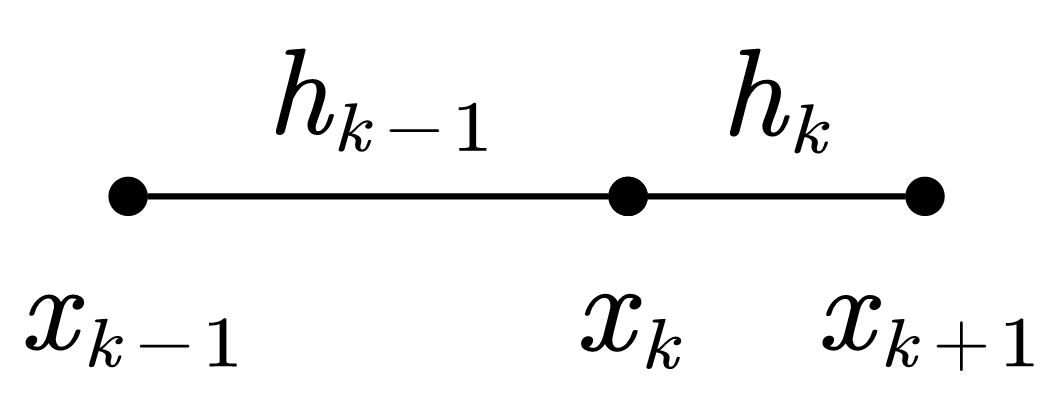
\includegraphics[width=3cm]{figure/Hingding-nonuniform-grid.png}
\end{center}

\subsection{二维}
\subsubsection{一致网格}
\paragraph*{梯度与Hessian阵}
\begin{empheq}{align}
\left.\pdv[order=2]{f}{x}\right|_{i,j}&=\frac{f_{i+1,j}-2f_{i,j}+f_{i-1,j}}{h^2}+\mathcal{O}(h^2)\\
\left.\pdv[order=2]{f}{y}\right|_{i,j}&=\frac{f_{i,j+1}-2f_{i,j}+f_{i,j-1}}{k^2}+\mathcal{O}(k^2)\\
\left.\pdv[order={1,1}]{f}{x,y}\right|_{i,j}&=\frac{f_{i+1,j+1}-f_{i+1,j-1}-f_{i-1,j+1}+f_{i-1,j-1}}{4hk}\mtag{四对角}\\
&=\frac{f_{i+1,j+1}-f_{i+1,j}-f_{i,j+1}+2f_{i,j}-f_{i-1,j}-f_{i,j-1}+f_{i-1,j-1}}{2hk}\mtag{七对角}
\end{empheq}
以上$f_{i+1,j+1}=f(x+h,y+k)$,其它类似。

注意在$f_{xy}$的第二个公式中,假如我们是依次计算$f_x,f_y,f_{xx},f_{yy}$,那么只需要再计算$f(x+h,y+k),f(x-h,y-k)$就可以计算$f_{xy}$了,$f(x+h,y)$一类可以利用之前计算的值。前两个$f_{xx},f_{yy}$实际上是固定另一个变量,然后进行一维差分。

图示如下:
\begin{center}
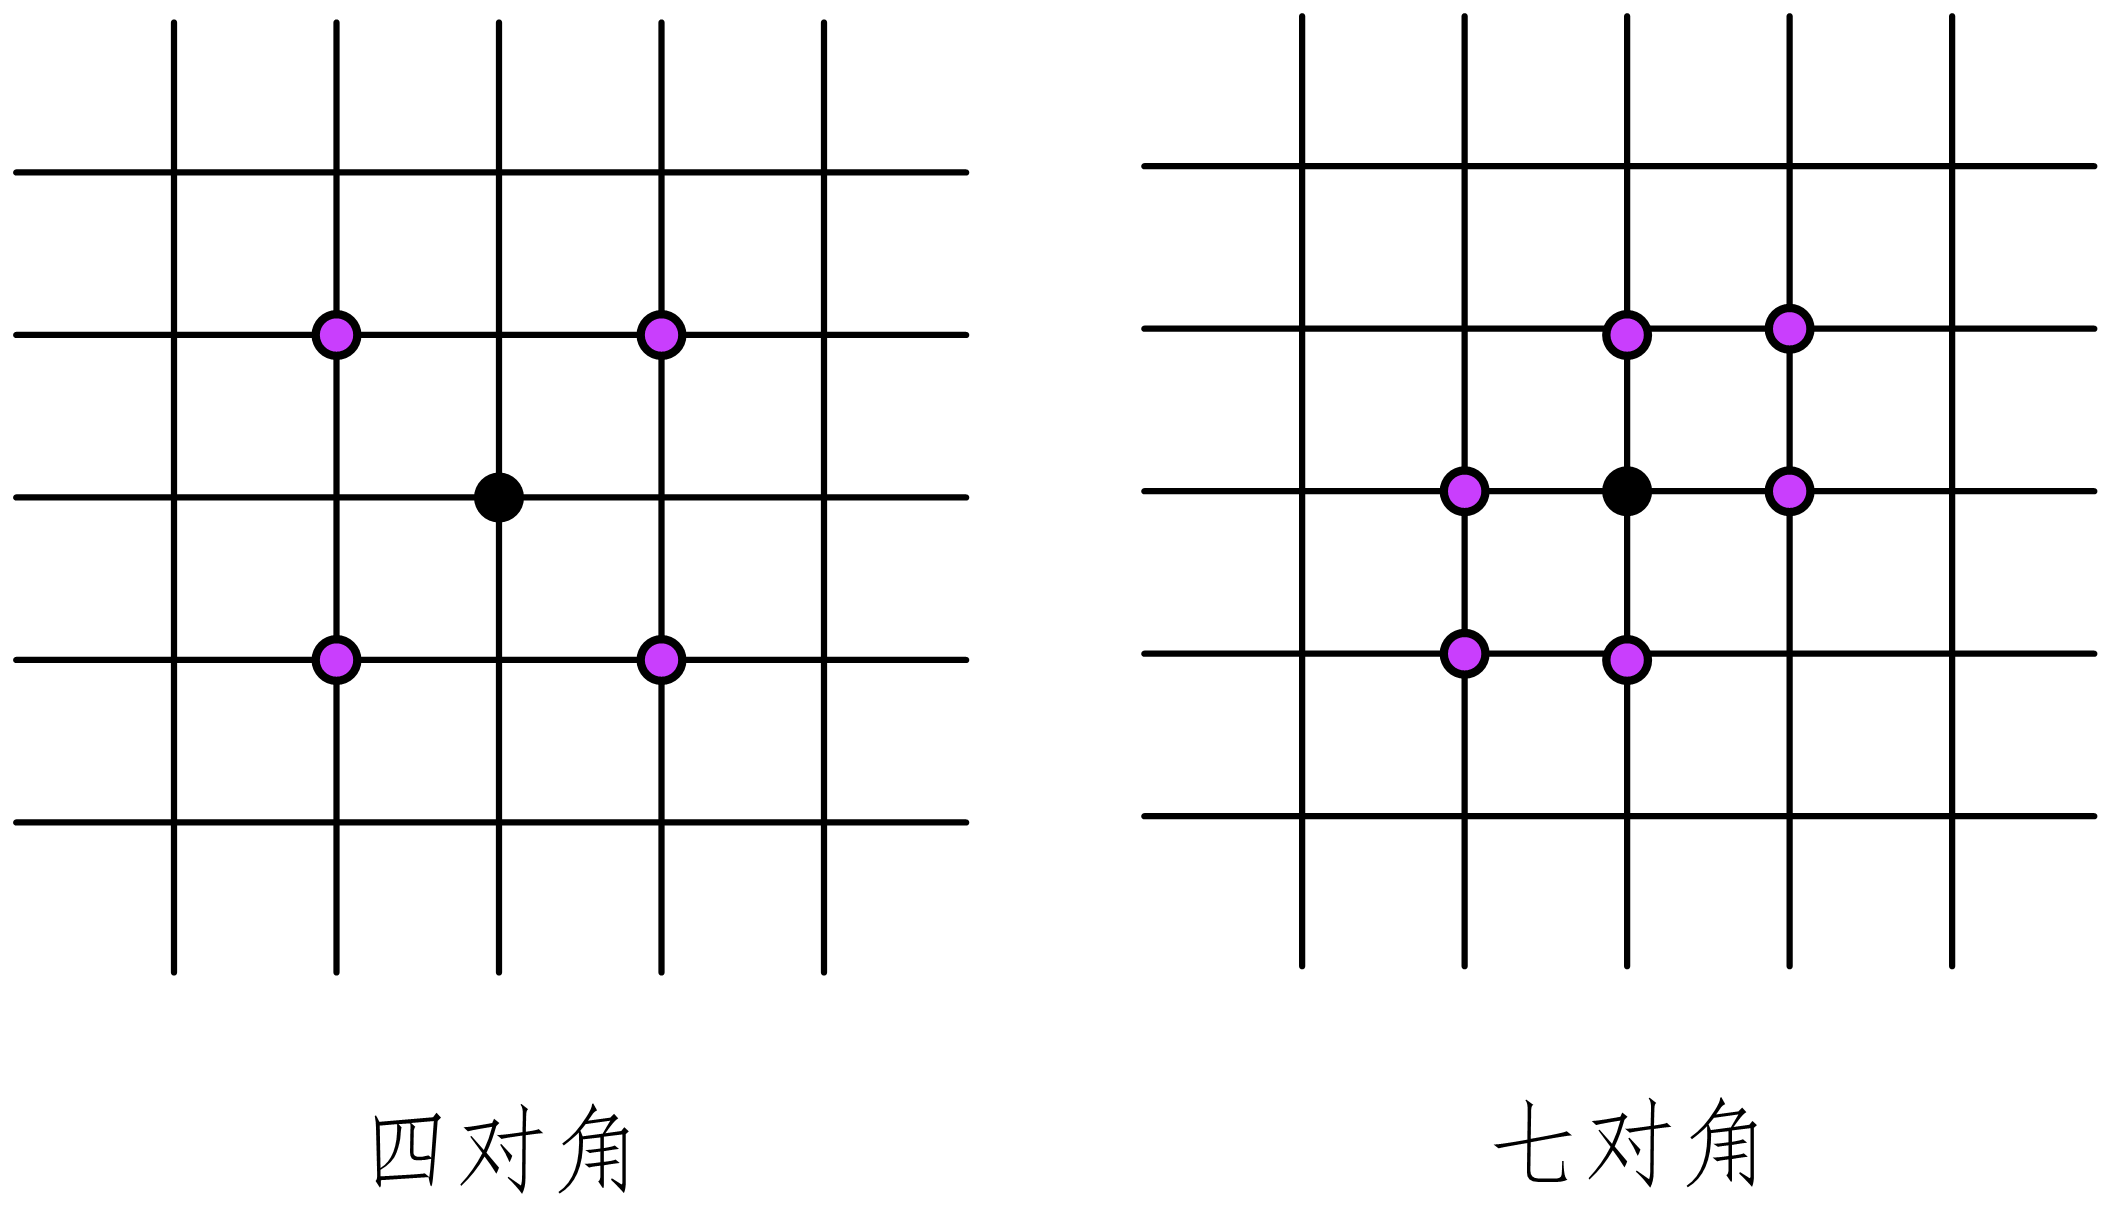
\includegraphics[width=10cm]{figure/2D-uniform-finite-difference.png}
\end{center}

\paragraph*{Laplacian}
\begin{empheq}{align}
\nabla^2 f|_{i,j}&=\left.\pdv[order=2]{f}{x}\right|_{i,j}+\left.\pdv[order=2]{f}{x}\right|_{i,j}-\inv{12}hk(f_{xxxx}+f_{yyyy})+\mathcal{O}(h^2k^2)\mtag{五点式}\\
&=\inv{6hk}(4f_{i-1,j}+4f_{i+1,j}+4f_{i,j-1}+4f_{i,j+1}\mtag{九点式}\\
&\qquad +f_{i-1,j-1}+f_{i-1,j+1}+f_{i+1,j-1}+f_{i+1,j+1}-20f_{i,j})\nonumber\\
&\qquad -\inv{12}hk(f_{xxxx}+2f_{xxyy}+f_{yyyy})+\mathcal{O}(h^2k^2)\nonumber
\end{empheq}
这里的五点式是指二阶导数用前面的中心差分。九点式已经把周围的点全用上了。

在9点式中,注意
\begin{empheq}{align}
f_{xxxx}+2f_{xxyy}+f_{yyyy}=\nabla^2(\nabla^2f)
\end{empheq}
所以可以在不求得解的情况下计算主误差。

\subsubsection{非一致网格}

\subsection{三维}
\subsubsection{一致网格}

\subsubsection{非一致网格}

\section{特殊微分与导数}
\subsection{Frechet导数}
\subsubsection{定义}

\subsection{Gateaux导数}

\subsection{Dini导数}

\section{微分算子}
\subsection{流与向量场}
\subsubsection{向量场}\label{vector-field}
\begin{definition}[向量场]
一个向量场是一个光滑映射:
$$X:U\rightarrow \Rns$$
其中$U\subset \Rns$是一个开集。

考虑一个对应的ODE:
$$\by'=X(\by),\by(0)=\bx$$
它的解$\by(t):\mathbb{R}\rightarrow\Rns$被称为向量场的积分曲线,或者轨道。同时记解
$$\by=\by(t,\bx)=\mathcal{F}_X^t(\bx)$$
这里的$\bx$是初值,是定值。$\mathcal{F}_X^t$被称为向量场产生的流,所以流是向量场的积分。

向量场定义了一个标量函数的微分算子:
$$\mathcal{L}_Xf(\bx)=\lim_{h\rightarrow 0}\frac{f(\mathcal{F}_X^t\bx)-f(\bx)}{h}=\left.\odv{}{t}f(\mathcal{F}_X^t\bx)\right|_{t=0}$$
也记为$\mathcal{L}_X f(\bx)=Xf$。根据微分法则有:
$$\mathcal{L}_X f(\bx)=X(\bx)\cdot \nabla f(\bx)=\sum a_j(\bx)\pdv{f}{x_j}$$
\end{definition}
把向量场作为速度场,在空间中选择一个起点$\bx$,在速度场的作用下进行运动,在空间中画出一条轨迹,就是流。

$\mathcal{L}_X f(\bx)$可以理解为:在微小的时间内,在速度场的作用下从一个点运动到另一个点,由此引起了标量函数的变化,从而可以定义导数。

\subsubsection{李导数}
\begin{definition}[李导数]

\end{definition}
\subsection{微分形式}
\subsubsection{$k$形式}
\begin{definition}[1-形式]
一个$\Omega\in\Rns$上的1-形式表示为
$$\alpha=\sum_j a_j(\bx)\dif x_j$$
假如$\gamma:[a,b]\rightarrow \Omega$是一条光滑曲线,则有
$$\int_{\gamma} \alpha=\int_a^b \sum_j a_j(\gamma(t))\gamma_j'(t)\dif t=\int_I \gamma^{\ast}\alpha$$
$\gamma^{\ast}$是$\alpha$在映射$\gamma$下的拉回。
\end{definition}

\begin{definition}[$k$-形式]
一个$\Omega$上的$k$-形式$\alpha$是一个向量场上的$k$重多线性映射:
$$\alpha(X_1,\cdots,X_k)\in C^{\infty}(\Omega)$$
它满足反对称性:
$$\alpha(X_,\cdots,X_j,\cdots,X_l,\cdots,X_k)=-\alpha(X_,\cdots,X_l,\cdots,X_j,\cdots,X_k)$$

$k$-形式记为
\begin{empheq}{equation}\label{diff-k-form}
\alpha=\sum_j a_j(\bx)\dif x_{j_1}\wedge\cdots\wedge \dif x_{j_k}
\end{empheq}
其中
$$a_j(\bx)=\alpha(D_{j_1},\cdots,D_{j_k}),\quad D_j=\pdv{}{x_j}$$
求和是对所有$k$-元组$(j_1,\cdots,j_k)$进行的,同时有:
$$\dif x_{j_1}\wedge \cdots \wedge \dif x_{j_k}=(\sgn \sigma)\dif x_{j_{\sigma(1)}}\wedge \cdots\wedge\dif x_{j_{\sigma(k)}}$$
$\sigma$是$\{1,\cdots,k\}$的一个排列。如果$j_m=j_l$,则上式为0。

一个$k$-形式也记为
$$\alpha\in\Lambda^{k}(\Omega)$$
\end{definition}

\subsubsection{微分形式的运算}
\paragraph*{外积}相当于微分形式的“乘法”。
\begin{definition}[外积wedgep product] 
假如$\alpha\in\Lambda^k(\Omega)$由\ref{diff-k-form}给出,而
$$\beta=\sum_i b_i(\bx)\dif x_{j_1}\wedge\cdots\wedge\dif x_{i_l}\in\Lambda^l(\Omega)$$
则有外积
$$\alpha\wedge\beta=\sum_{j,i}a_j(\bx)b_i(\bx)\dif x_{j_1}\wedge\cdots\wedge\dif x_{j_k}\wedge\dif x_{i_1}\wedge\cdots\wedge\dif x_{i_l}=(-1)^{kl}\beta\wedge\alpha$$
对于一些特殊情形有以下记号:
$$\wedge_k \alpha=\dif x_k\wedge\alpha$$
\end{definition}
上面$a_jb_i$的形式有点类似于向量的外积$\bx\by^T$,而$\dif$项是直接拼在一起的。

\paragraph*{内积}此“内积”(interior product)不是Hilbert空间中的内积。
\begin{definition}[内积interior product]
也叫contraction。定义为
$$(\alpha\rfloor X)(X_1,\cdots,X_{k-1})=\alpha(X,X_1,\cdots,X_{k-1})\in\Lambda^{k-1}(\Omega)$$
也可以记为$i_X\alpha$。

特殊记号:
$i_k\alpha=\alpha \rfloor D_k$。
\end{definition}
contraction可能比interior product更加形象。有点类似于消去一个参数。在Matlab中定义function handle的时候有类似的操作:
\begin{center}
\texttt{new\_fun=@(y) fun(x,y)}
\end{center}


\paragraph*{外微分}对微分形式进行微分。
\begin{definition}[外微分exterior derivative]
外微分$d:\Lambda^k(\Omega)\rightarrow\Lambda^{k+1}(\Omega)$定义为:
$$\dif \alpha=\sum_{j,l}\pdv{a_j}{x_l}\dif x_l\wedge x_{j_1}\wedge\cdots\wedge \dif x_{j_k}$$

它满足性质
\begin{enumerate}
\item $\dif(\dif \alpha)=0$。
\item $\dif(\alpha\wedge\beta)=(\dif \alpha)\wedge \beta+(-1)^k\alpha\wedge(\dif\beta),\quad\alpha\in\Lambda^k(\Omega),\beta\in\Lambda^j(\Omega)$
\item $F^{\ast}(\dif\alpha)=\dif (F^{\ast}\alpha)$
\end{enumerate}
\end{definition}

外微分有一个著名的定理:
\begin{theorem}[外微分定理]
\begin{empheq}{equation}
\int_{\Omega}\dif \alpha=\int_{\partial \Omega} \omega
\end{empheq}
\end{theorem}
它把全区域的积分转换成了边界上的积分,牛顿-莱布尼茨公式、格林公式、高斯公式都是它的特例。
\paragraph*{关系}
\begin{empheq}{align}
\wedge_k \iota_l+\iota_l\wedge_k&=\delta_{kl}\mtag{反交换}\\
\wedge_j\wedge_k+\wedge_k\wedge_l&=0\\
\iota_j\iota_k+\iota_k\iota_j&=0
\end{empheq}

\subsection{Halmiltonian系统}


\section{一元积分}
注意有的文章里面没有使用标准符号,比如\cite{10.2307.3215821}中,
$$\int_{0}^{\infty}\dif h\ G(h)$$
其实是表示 
$$\int_{0}^{\infty}G(h)\dif h$$
而不是
$$\int_{0}^{\infty}\dif (hG(h))$$
\subsection{定积分}
\subsubsection{微积分基本公式}
\begin{empheq}{equation}
\int_{a}^{b}\dif F(x)=F(b)-F(a)
\end{empheq}
\section{曲线积分}
\subsection{对线元曲线积分}
对线元的积分:
\begin{empheq}{equation}
\int_L f(\bx)\dif s
\end{empheq}
$L$是一段曲线,$\dif s$为线元。

在曲线自然参数化下,曲线表示为弧长的函数:$L=\bx(s)$,此时原积分为
$$\int_{s_0}^{s_1} f(\bx(s))\dif s$$

假如曲线可以由参数曲线$L=\bx(t)$,则$\dif s=\sqrt{\sum \left(\odv{x_k}{t}\right)^2}$,则原积分为:
$$\int_{t_0}^{t_1} f(\bx(t))\sqrt{\sum \left(\odv{x_k}{t}\right)^2}\dif t$$

假如曲线可以转化为某个坐标$x_i$的函数则原积分为:
$$\int_{x_0}^{x_1} f(\bx(x_i))\sqrt{\sum \left(\odv{x_k}{x_i}\right)^2}\dif x_i$$
跟$t$参数化是一回事。

假如曲线可以由一个单参数化经过坐标变换给出:$L=\bx(\by(t)))$。则$\dif \bx=J\by'\dif t$,$\dif s=\sqrt{(\dif \bx)^T(\dif \bx)}=\sqrt{(\by')^TJ^TJ\by'}\dif t=\sqrt{g_{ij}\dif y^i\dif y^j}$。参考\ref{tensor-field-metric}。

比如对于极坐标系,$t=\theta,\by=(r,\theta),\by'=(r',1)$,有
$$\int_L f(x,y)\dif s=\int_{\theta_0}^{\theta_1}f(r(\theta)\cos\theta,r(\theta)\sin\theta)\sqrt{r^2(\theta)+(r'(\theta))^2}\dif \theta$$
\subsection{对坐标曲线积分}
对坐标的积分:
$$\int_L \sum a_k(\bx)\dif x_k$$
这个一般可以每一项分开算,把曲线$L$分别转换成$x_k$的函数,然后再当成一元积分。

也可以常规换元:
$$\int_{t_0}^{t_1}\sum a_k(\bx(t))x_k'\dif t$$

\subsection{联系与区别}
\begin{enumerate}
\item 第一类曲线积分与第二类曲线积分可以相互转化:
$$\int_L \sum a_k(\bx)\dif x_k=\int_L \sum a_k(\bx)\cos\theta_k\dif s$$
$\theta_k$为有向曲线弧的单位切向量。实际上给定一个向量$\dif s$,则它在某方向的投影长就是$(\dif s)\theta_k=\dif x_k$,所以上式也相当于换元。
\end{enumerate}
\subsection{例题}

\section{重积分}
\subsection{二重积分}
\subsubsection{一般二重积分}
\paragraph*{一般形式}笛卡尔坐标系下:
\begin{empheq}{equation}
\int_{\Omega}f(x,y)\dif x\dif y=\int_{x_0}^{x_1}\int_{y_0(x)}^{y_1(x)}f(x,y)\dif y\dif x
\end{empheq}

极坐标系下:
\begin{empheq}{equation}
\int_{\Omega}f(r,\theta)r\dif r\dif \theta=\int_{\theta_0}^{\theta_1}\int_{r_0(\theta)}^{yr_1(\theta)}f(r,\theta)r\dif r\dif \theta
\end{empheq}

\subsubsection{对面积曲面积分}
\paragraph*{基本形式}
\begin{empheq}{equation}
\int_{\Sigma} f(x,y,z)\dif S
\end{empheq}
这里的$\dif S$是曲面上一个小的面积元,注意它不是$\dif x\dif y$。 
\paragraph*{投影法}假如$\Sigma$可以投影到某个坐标面上,比如$xOy$,则有
\begin{empheq}{equation}\label{2d-int-area-project}
\int_{\Sigma} f(x,y,z)\dif S=\int_{D_{xy}}f(x,y,z(x,y))\sqrt{1+z_x^2+z_y^2}\dif x\dif y
\end{empheq}

\subsubsection{对坐标曲面积分}
\paragraph*{基本形式}
\begin{empheq}{equation}
\int_{\Sigma} f(x,y,z)\dif x\dif y
\end{empheq}
\paragraph*{投影法}假如$\Sigma$可以投影到某个坐标面上,比如$xOy$,则有
\begin{empheq}{equation}
\int_{\Sigma} f(x,y,z)\dif x\dif y=\pm\int_{D_{xy}}f(x,y,z(x,y))\dif x\dif y
\end{empheq}
注意与面积的曲面积分式\cref{2d-int-area-project}不同,被积表达式没有根号那一项。而且符号有正负。一般外法向定义为正。 

\subsubsection{两类曲面积分的联系}
\paragraph*{基本原理}
\begin{empheq}{equation}
\int_{\Sigma} P\dif y\dif z+Q\dif x\dif z+R\dif x\dif y=\int_{\Sigma} P\cos\alpha+Q\cos\beta+R\cos\gamma\dif S
\end{empheq}

\subsubsection{格林公式}\label{green-formula}
\paragraph*{基本原理}把二维封闭曲面积分转换成边界上的二维曲线积分:
\begin{empheq}{equation}
\int_{\Omega}\left(\pdv{Q}{x}-\pdv{P}{y}\right)\dif x\dif y=\int_{L^+}  P\dif x+Q\dif y
\end{empheq}
这里的$L^+$表示正向,沿着曲线走,曲面总在左边的方向为正,直观就是逆时针。

\paragraph*{有限元基本公式}以下假定$\Omega$为一平面区域。这个积分出现在拉普拉斯方程的有限元法中:
\begin{empheq}{align}
\langle -\Delta u, v\rangle&=\iint_{\Omega} v\Delta u\dif x\dif y\\
&=-\iint_{\Omega} \left(\underbrace{((u_xv)_x+(u_y v)_y)}_{\text{格式公式}}-u_xv_x-u_yv_y\right)\dif x\dif y\\
&=-\int_{\partial \Omega} u_x v\dif y-u_y v\dif x+\iint_{\Omega} u_xv_x+u_yv_y\dif x\dif y
\end{empheq}

假如$u,v$在边界$\partial \Omega$上为0,则原式变成:
\begin{empheq}{equation}
\langle -\Delta u, v\rangle=\iint_{\Omega} u_xv_x+u_yv_y\dif x\dif y
\end{empheq}

\subsubsection{斯托克斯公式}\label{2d-surface-int-stokes-theorem}
\paragraph*{基本原理}把三维封闭曲面积分转换成边界上的三维曲线积分:
\begin{empheq}{align}
&\int_{\Sigma}\left(\pdv{R}{y}-\pdv{Q}{z}\right)\dif y\dif z+\left(\pdv{P}{z}-\pdv{R}{x}\right)\dif x\dif z+\left(\pdv{Q}{x}-\pdv{P}{y}\right)\dif x\dif y\\
=&\int_{\Sigma}\begin{vmatrix}
\dif y \dif z& \dif z\dif x & \dif x\dif y \\
P & Q& R\\
\pdv{}{x}& \pdv{}{y}&\pdv{}{z}
\end{vmatrix}\\
=&\int_{L^+} P\dif x+Q\dif y+R\dif z
\end{empheq}
这里的正向符合右手法则:除大拇指外手指绕曲线时,大拇指指的方向为正向。

\subsubsection{曲面面积}
\paragraph*{面积的计算}熟知一个平面曲面$D$的面积在笛卡尔系下表示为:
\begin{empheq}{align}
S=\iint_{D}\dif x\dif y=\int_{x_0}^{x_1}\int_{y_0(x)}^{y_1(x)}\dif y\dif x
\end{empheq}

在极坐标系下为:
\begin{empheq}{align}
S=\iint_{D}r\dif r\dif \theta=\int_{\theta_0}^{\theta_1}\int_{r_0(\theta)}^{r_1(\theta)}r\dif r\dif \theta
\end{empheq}
但使用极坐标计算务必需要$\Sigma$包含原点,且为简单曲面。否则会出错。

如果使用斯托克斯公式\ref{2d-surface-int-stokes-theorem},则面积可以改写为:
\begin{empheq}{align}
S&=\iint_{D}\dif x\dif y\\
&=-\oint_{L^+}y\dif x\\
&=\oint_{L^+} x\dif y\\
&=\inv{2}\oint_{L^+} x\dif y-y\dif x
\end{empheq}
这样就转换成了一个曲线积分的问题,假如曲面是由参数方程给出的,则计算较为方便。但务必注意曲线不能自交。

\paragraph*{参数曲面算例}
\begin{example}
考虑一个参数曲面:$x=\cos 2t,y=t\sin t,0\leq t\leq 2\pi$所围图形的面积。

该参数曲线如下图所示:
\begin{center}
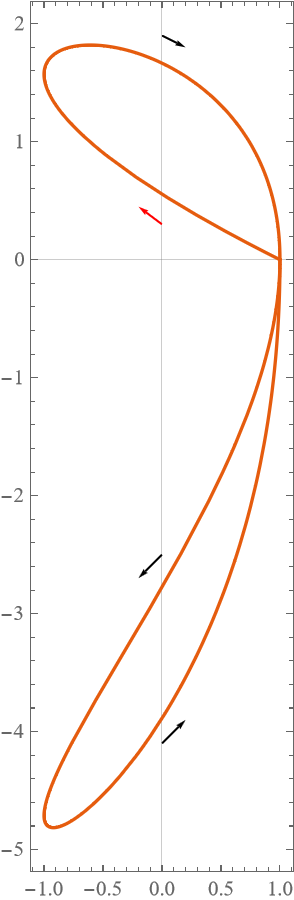
\includegraphics[width=4cm]{figure/two-curve.png}
\end{center}
红色箭头为起始方向。
\end{example}
\begin{solution}
由于曲线是自交的,所以需要分两段计算。
\begin{empheq}{align*}
S&=-\left(-\int_{0}^{\pi} y\dif x\right)-\int_{\pi}^{2\pi}y\dif x\\
&=-2\int_{0}^{\pi}t\sin t \sin (2t)\dif t +2\int_{\pi}^{2\pi}t\sin t \sin (2t)\dif t\\
&=\frac{16}{9}+\frac{16}{9}\\
&=\frac{32}{9}
\end{empheq}
第一项的前面有个负号,是因为沿图中红色箭头方向出发时,曲面在右边,但曲面在左边时才定义为正,所以需要取反。
\end{solution}
\subsection{三重积分}
\subsubsection{一般三重积分}
\paragraph*{基本形式}
\begin{empheq}{equation}
\int_{\Omega}f(x,y,z)\dif V=\int_{x_0}^{x_1}\int_{y_0(x)}^{y_1(x)}\int_{z_0(x,y)}^{z_1(x,y)}f(x,y,z)\dif z\dif y\dif x
\end{empheq}
上式中$\dif V=\dif x\dif y\dif  z$,物理学中有时也记为$\dif^3 x$。

\paragraph*{球坐标}

\subsubsection{高斯公式}
\paragraph*{基本原理}高斯公式建立了体积分与曲面积分的联系,把体积分变成边界上的对坐标曲面积分。 
\begin{empheq}{equation}
\int_{\Omega}\left(\pdv{P}{x}+\pdv{Q}{y}+\pdv{R}{z}\right)\dif x\dif y\dif z=\int_{\partial\Omega}  P\dif y\dif z+Q\dif x\dif z+R\dif x\dif y
\end{empheq}

\paragraph*{泊松方程3D有限元基本公式}以下$\Omega$为一3D区域。积分出现在3D泊松方程的有限元法中,利用高斯公式可以证明:
\begin{empheq}{align}
\langle -\Delta u,v\rangle &=-\iiint_{\Omega} v\Delta u\dif V\\
&=-\iiint_{\Omega} (u_xv)_x+(u_yv)_y+(u_zv)_z-(u_xv_x+u_yv_y+u_zv_z)\dif V\\
&=-\iint_{\partial \Omega} u_xv\dif y\dif z +u_yv\dif x\dif z+u_zv\dif x\dif y+\iiint_{\Omega}\nabla u\cdot\nabla v\dif V
\end{empheq}

假如在边界上$v$为0,则
\begin{empheq}{equation}
\langle -\Delta u,v\rangle =\iiint_{\Omega}\nabla u\cdot\nabla v\dif V
\end{empheq}


\subsubsection{旋转体}

\section{数值积分}
\subsection{插值型求积}
\subsubsection{简介}

\subsubsection{牛顿-柯茨法}

\subsubsection{高斯求积}

\subsection{复化求积}
\subsubsection{基本原理}
对于一维函数,把区间$[a,b]$分隔为多个小区间得到节点$[x_0,\cdots,x_n]$,在每个小区间上进行近似:
\begin{empheq}{equation}
I=\int_{a}^{b} f(x)\dif x=\sum_{k=0}^{n-1} \int_{x_k}^{x_{k+1}} f(x)\dif x
\end{empheq}
小区域积分$\int_{x_k}^{x_{k+1}} f(x)\dif x$可以用前面的插值型积分来计算。
\subsubsection{梯形法则}
用梯形来逼近积分:
\begin{empheq}{equation}
\int_{x_k}^{x_{k+1}} f(x)\dif x=\frac{(f(x_k)+f(x_{k+1}))(x_{k+1}-x_k)}{2}
\end{empheq}

\section{积分表}
\subsection{基本函数}

\subsection{三角函数}
\begin{align}
\int_{-\infty}^{\infty} \frac{\sin^2 x}{x^2}\dif x&=\pi
\end{align}

\subsection{超越函数}

\subsection{有理函数}

\subsection{无理函数}
\begin{empheq}{align}
\int \frac{\dif x}{\sqrt{ax^2+bx+c}}&=\inv{\sqrt{a}}\ln\left(\sqrt{ax^2+bx+c}+\sqrt{a}x+\frac{b}{2\sqrt{a}}\right)+C
\end{empheq}
\chapter{特殊函数}
\section{Gamma族函数}
\begin{empheq}{align*}
	\Gamma(x) & =\int_{0}^{\infty} t^{x-1}e^{-t} \dif t=(x-1)! \\
	\text{Beta}(x,y) & =\int_{0}^{1} t^{x-1}(1-t)^{y-1} \dif x=\frac{\Gamma(x)\Gamma(y)}{\Gamma(x+y)}\\
	\Gamma_p(x)&=\pi^{\frac{p(p-1)}{4}}\prod_{k=1}^{p}\Gamma\left(x-\frac{k-1}{2}\right)\mtag{Multivariate Gamma}\\
	\Gamma_1(x)&=\Gamma(x)\\
	\Gamma_2(x)&=\pi^{\frac{1}{2}}\Gamma(x)\Gamma\left(x-\frac{1}{2}\right)\\
	\psi(x)&=\frac{\partial \ln \Gamma(x)}{\partial x}=\frac{\Gamma'(x)}{\Gamma(x)} \mtag{digamma}\label{digamma}\\
	\psi_1(x)&=\psi'(x)=\frac{\partial^2 \ln\Gamma(x)}{\partial^2 x} \mtag{Trigamma}
\end{empheq}
在Mathematica中Digamma函数用\texttt{PolyGamma[z]}计算,Trigamma函数用\texttt{PolyGamma[1,z]}表示。
\section{Bessel}
常微分方程:

$$y''+\frac{1}{z}y'+(1-\frac{v^2}{z^2})y=0$$

它的解为:

\begin{empheq}{align*}
	J_v(z) &=\sum_{k=0}^{\infty}(-1)^k\frac{1}{k!\Gamma(v+k+1)}\left(\frac{z}{2}\right)^{2k+v} \\
	I_v(z) &=\sum_{k=0}^{\infty}\frac{1}{k!\Gamma(v+k+1)}\left(\frac{z}{2}\right)^{2k+v} \\
	K_v(z) &=\frac{\pi}{2\sin v\pi}(I_{-v}(z)-I_v(z))
\end{empheq}

\section{超几何函数}

\begin{empheq}{align*}
	F(\alpha,\beta,\gamma,x) &=\sum_{k=0}^{\infty} \frac{(\alpha)_k(\beta)_k}{(\gamma)_k k!}z^n\\
	&=\sum_{k=0}^{\infty}\frac{\Gamma(\alpha+k)\Gamma(\beta+k)\Gamma{\gamma}}{\Gamma(\alpha)\Gamma(\beta)\Gamma(\gamma+k)\Gamma(k+1)}z^k
\end{empheq}

其中$(\alpha)_0=1,(\alpha)_n=\alpha(\alpha+1)\cdots(\alpha+n+1)=\frac{\Gamma(\alpha+n)}{\Gamma(\alpha)}$.

\section{椭圆函数}
\begin{empheq}{align*}
t=\sn(u,k) &\Longleftrightarrow u=\int_{0}^{t}\frac{\dif t}{\sqrt{(1-t^2)(1-k^2t^2)}}\\
\varphi=\am (u,k) &\Longleftrightarrow u=\int_{0}^{\varphi}\frac{\dif \varphi}{\sqrt{1-k^2\sin^2 \varphi}}
\end{empheq}

有以下关系:

\begin{empheq}{align*}
\sn u&=\sin \am u\\
\cn u&=\cos \am u\\
\dn u&=\sqrt{1-k^2\sn^2u}\\
\sn^2 u+\cn^2 u&=1\\
\dn^2u+k^2\sn^2u&=1
\end{empheq}

\section{Polylogarithm函数$\Li_s(z)$}
Polylogarithm函数:
$$\Li_s(z)=\sum_{k=1}^{\infty}\frac{z^k}{k^s}$$

其积分表示为:
$$\Li_{s+1}(z)=\int_{0}^{\infty}\frac{\Li_s(t)}{t}\dif t$$

又叫费米-狄拉克积分或玻色-爱因斯坦积分.

特殊值:
\begin{empheq}{align*}
\Li_1(z)&=-\ln(1-z)
\end{empheq}

\section{三角积分、对数与指数积分}
\begin{empheq}{align*}
\li(x)&=\int_{0}^{x}\frac{\dif t}{\ln x}=\Ei(\ln x)\mtag{对数积分}\\
\Li(x)&=\li(x)-\li(2) \mtag{欧拉对数积分}\\
\Ei(x)&=\int_{-\infty}^{x}\frac{e^t}{t}\dif t \mtag{指数积分}\\
\E_1(z)&=\int_{1}^{\infty}\frac{e^{-zt}}{t}\dif t\\
\Si(x)&=\int_{0}^{x}\frac{\sin t}{t}\dif t\mtag{正弦积分}\\
\isi(x)&=-\int_{x}^{\infty}\frac{\sin t}{t}\dif t\mtag{正弦积分}\\
\ci(x)&=-\int_{x}^{\infty}\frac{\cos t}{t}\dif t\mtag{余弦积分}\\
\end{empheq}

$\li(x)=0$的唯一正值解叫拉马努金-索德纳常数,值$\gamma\approx 1.45$.

特殊值:
\begin{empheq}{align*}
\E_1(ix)&=i\si x-\ci x\\
\end{empheq}

\section{正交多项式}
\subsection{勒让德多项式}
微分方程
$$\left[(1-x^2)y'\right]'+l(l+1)y=0$$
的解称为勒让得多项式:
$$y=P_l(x)=\frac{1}{2^ll!}\odv[order={l}]{}{x}(x^2-1)^l$$

另外有\textbf{连带勒让德多项式}:
$$P_l^m(x)=(-1)^m(1-x^2)^{m/2}\odv[order={m}]{P_l(x)}{x}$$

\section{球谐函数}
来自球坐标系下的拉普拉斯方程。

$$Y_{l,m}(\theta,\phi)=\sqrt{\frac{2l+1}{4\pi}\frac{(l-m)!}{(l+m)!}}P_l^m(\cos\theta)e^{im\phi}$$

一些特殊值:
\begin{enumerate}
\item $Y_{0,0}=\sqrt{\frac{1}{4\pi}}$
\item $Y_{1,0}=\sqrt{\frac{3}{4\pi}}\cos\theta$。
\end{enumerate}
\chapter{级数、有理函数与函数逼近}\label{series-function-approxmation}
\section{子空间逼近}
\subsection{逼近的定义}

\subsection{正交子空间逼近}
\subsubsection{一维正交子空间逼近}
给定一个$[0,1]$上的线性正交函数空间$V_n=\{1,g_1(x),g_2(x),\cdots\}$,所谓正交是指:
$$\int_{0}^{1} g_i(x)g_j(x)\dif x=\delta_{ij}$$
假如有一个函数$f$,则它的最佳逼近(或称其为投影)为:
$$f(x)=\sum a_i g_i(x),\quad a_i=\int_{0}^{1}f(x)g_i(x)\dif x$$

这是因为
$$\int_0^{1}f(x)g_i(x)\dif x=\int_{0}^{1}a_ig_i(x)g_i(x)\dif x =a_i$$
\subsubsection{常见一维正交多项式空间}

\subsection{泰勒公式}
\subsubsection{一维}
\paragraph*{标准公式}
\begin{empheq}{align*}\label{1d-taylor}
f(x)&=\sum_{k=0}^{\infty}\frac{f^{(k)}(x_0)}{k!}(x-x_0)^k\\
&=f(x_0)+f'(x_0)(x-x_0)+\inv{2}f''(x_0)(x-x_0)^2+\cdots
\end{empheq}
\subsubsection{典型例子}
为了方便阅读,以下所有结果中级数求和从$k=0$开始。

\paragraph*{初等函数}
\begin{empheq}{align}
\ln(1+x)&=\sum_{k=0}^{\infty}\frac{(-1)^{k}x^{k+1}}{k+1}\approx x-\inv{2}x^2+\inv{3}x^3\\
\ln\left(\frac{1+x}{1-x}\right)&=2\sum_{k=0}^{\infty}\frac{x^{2k+1}}{2k+1},|x|<1
\end{empheq}
\begin{empheq}{align}
\arctan x&=\sum_{k=0}^{\infty}\frac{(-1)^kx^{2k+1}}{2k+1}\approx x-\inv{3}x^3,|x|<1
\end{empheq}

\subsubsection{高维}
\paragraph*{$\Rns\rightarrow \mathbb{R}$}二阶逼近:
\begin{empheq}{equation}\label{nd-taylor}
f(\bx)\approx f(\bx_0)+\nabla f(\bx_0)(\bx-\bx_0)+\inv{2}(\bx-\bx_0)^T\nabla^2 f(\bx_0)(\bx-\bx_0)
\end{empheq}
\subsubsection{典型例子}

\subsection{常用的逼近公式}
\subsubsection{函数逼近}
\begin{empheq}{align*}
n!&=\sqrt{2\pi n}\left(\frac{2\pi}{e}\right)^n\left(1+O\left(\frac{1}{n}\right)\right) \mtag{Stirling公式}\\
\ln x&\approx 1-x,\ x\rightarrow 1
\end{empheq}

\subsection{基本级数}
\subsubsection{加法}
\begin{empheq}{align*}
e^x&=\sum_{k=0}^{\infty} \frac{x^k}{k!},\quad |R|=\infty\\
\frac{1-x^{n+1}}{1-x}&=\sum_{k=0}^{n}x^k\\
\inv{a+x}&=\sum_{k=0}^{\infty} \inv{a^{k+1}}x^k,\quad |R|=\inv{a},a>0\\
&\approx 1-x+x^2-x^3+\cdots\\
\sum_{n=0}^{\infty}\frac{(-1)^n}{n+1/2}&=\frac{\pi}{2}\\
\sum_{n=1}^\infty \frac{(-1)^n}{n}&=\sum_{n=1}^{\infty}\frac{(-1)^n}{n}x^n\rvert_{x=1}=-\ln|1+x|\rvert_{x=1}=-\ln 2
\end{empheq}
\subsubsection{乘法}


\section{有理函数}
\subsection{Pade逼近}
\subsubsection{定义}
\begin{definition}[Pade逼近]
给定一个连续函数$f$和两个整数$m,n$,则$f$的Pade逼近定义为:
\begin{empheq}{equation}
R(x)=\frac{\sum_{k=0}^{m}a_kx^k}{1+\sum_{k=1}^{n}b_kx^k}
\end{empheq}
注意下面的求和是从1开始的。相当于分母的0次项为1。系数满足要求:
$$f^{(i)}(x)=R^{(i)}(x)$$


\end{definition}

\begin{property}
\item Pade逼近是{\heiti 唯一}的。
\item 将$R(x)$按级数展开后,前$m+n$项对应$f$直接展开时的项。
\end{property}
\subsubsection{常见函数的逼近}

\subsection{连分数}

\chapter{泛函分析}\label{functional-analysis}

\section{泛函分析重要概念}
\subsection{泛函分析思想}
\subsection{泛函分析中的空间}
\subsubsection{各种空间的图景}
\begin{center}
\includegraphics[width=14cm]{figure/Functional Space - Overview.png}
\end{center}
\subsubsection{拓扑空间}
\begin{definition}[拓扑空间]\label{}
拓扑空间是一个集合$X$及其子集族$\tau$,满足以下条件:

\begin{enumerate}
	\item 空集和$X$属于$\tau$.
	\item $\tau$中任意多个集合的交和并均属于$\tau$.
\end{enumerate}

称子集族$\tau$为$X$的拓扑.$\tau$中的元素称为开集.开集的补集为闭集,集合可以是开的、闭的、非开非闭、既开又闭.

集合$\{\emptyset,X\}$构成平凡拓扑.

给定两个拓扑空间$X,Y$和一个映射$f\colon X\rightarrow Y$,如果$Y$中开集的原像是$X$中的开集,则称$f$连续.如果$X$中开集的像在$Y$中是开集,称$f$为开映射.

$X$到$Y$的所有连续映射记为$\mathcal{C}(X;Y)$.
映射$f\colon X\rightarrow Y$称为$X$到$Y$上的同胚,如果$f$是双射,且$f\in\mathcal{C}(X;Y),f^{-1}\in \mathcal{C}(X;Y)$.此时又称$X$与$Y$同胚.
\end{definition}

与子集族$\tau$相近的一个概念是滤子.

\begin{definition}[滤子]\label{}
设$X$为一集合,$\mathcal{F}$是$X$的非空子集族,如果:
\begin{enumerate}
\item $\mathcal{F}$中任意两个元素的交属于$\mathcal{F}$.
\item 如果$A\in\mathcal{F},A\subset B\subset X$,那么$B\subset \mathcal{F}$.
\end{enumerate}	

\end{definition}
第一个性质是指$\mathcal{F}$对交运算完备(但不像拓扑空间中一样涉及并运算),第二个性质类似于扩张.滤子的概念与$\sigma$代数十分相似.

拓扑空间的例子有:距离空间.

拓扑空间可以有连续性(指映射连续)、紧性、连通性.之前的定义中已经确定了连续性.

\begin{definition}[拓扑空间的紧性]\label{}
拓扑空间$X$是紧的,是指对$X$中任何一族开集$(O_i)_{i\in I}$,当$K\subset \bigcup_{i\in I}O_i$时,必存在$(O_i)_{i\in I}$的有限子族$(O_j)_{j\in J}$,使得$K\subset \bigcup_{j\in J}O_j$.
	
一种等价描述性:任何开覆盖均有有限子覆盖.

这种性质又称为Heine-Borel-Lebesgue性质.

在欧几里得空间中,这又等价于集合封闭且有界.
\end{definition}

开覆盖是指$\bigcup_{i\in I}O_i$,有限子覆盖是指$\bigcup_{j\in J}O_j$.

乍看上去,紧性似乎对每个拓扑空间都应该成立.因为既然$K\subset \bigcup_{i\in I}O_i$,即$K$属于交集,那么这个交肯定是由子集族中一些集合相交得到的.

问题核心就在这个“有限”上.比如取区间$(0,1]$,它不是紧的,因为它有开覆盖$\big\{(\frac{1}{n},1]\big\}_{n=1}^\infty$.但它的任意子覆盖必然不能覆盖区间$(0,1]$.但区间$[0,1]$就是紧的,前述的开覆盖并不能覆盖它.

紧空间的一些好处有:
\begin{enumerate}
\item 紧空间上的连续函数必然有最大最小值.
\end{enumerate}


\begin{definition}[拓扑空间的连通性]\label{}
拓扑空间$(X,\mathcal{O})$是连通的,是指$X$中既是开集又是闭集的子集只有$X$和$\emptyset$.

等价于$X$不能被分为两个不相交开集的并.

$X$的子集$A$称为连通的,是指$A$关于$X$在$A$上的诱导拓扑,它是一个连通的拓扑空间.

设$x,y\in X$,从$x$到$y$中的道路是指连续映射$[0,1]\rightarrow X$,它满足$\gamma(0)=x,\gamma(y)=y$.如果任意两个不同的点存在道路,称$X$弧连通.
\end{definition}

连通性的等价定义更容易理解——不能分为不相交开集的并.比如两个不相交的圆取并形成的集合,就不是连通的.连通性可以诱导中值定理.

\begin{definition}[Bolzano中值定理]\label{}
$X$为连通拓扑空间,$f\colon X\rightarrow \mathbb{R}$为连续函数,$a,b\in X$且$f(a)<f(b)$,则对任意给定的$y\in]f(a),f(b)[$,存在$x\in X$,使得$f(x)=y$.
\end{definition}

通俗地说,中值定理是指连通拓扑空间上的连续函数可以取一切中间值.

对于一个特定的集合可以构造很多拓扑,但很多是没有用的,如果引入更多的公理(或者说约束),就能定义更好性质的拓扑.常见的有分离公理、可数性公理.

\begin{definition}{分离定理}{}
$T_0$公理:任意不同的两点,存在某点的开邻域,不包含另外一点.

$T_1$公理:任意不同的两点,每个点存在开邻域,不包含另外一点.

$T_2$公理:任意不同的两点,每个点存在互不相交的开邻域.

满足$T_2$公理的空间又称$T_2$空间、豪斯多夫空间.$T_2$空间中每个序列不会收敛到两点以上的点.度量空间都是$T_2$空间.
\end{definition}

从$T_0$到$T_2$是递进的,越来越严格.比如$T_1$公理中,邻域不包含另外一点,但可以相交.

\subsubsection{距离空间}
\paragraph*{距离空间}就是集合加上距离函数。
\begin{definition}[距离空间]\label{}
设$X$是一个集合,函数$d:X\times X\rightarrow \mathbb{R}$满足下列性质:$\forall x,y,z\in X$,
\begin{empheq}{align*}
d(x,x)&=0,\text{且如果}x\neq y,\text{则}d(x,y)>0\\
d(x,y)&=d(y,x)\\
d(x,z)&\leq d(x,y)+d(y,z)
\end{empheq}
$(X,d)$为距离空间。
\end{definition}
\paragraph*{完备距离空间}每个Cauchy序列均在$X$中收敛的距离空间,在$X$中收敛需要满足两个条件,一是收敛,二是收敛的点也在$X$中。
\begin{definition}[Cauchy列]
记$(X,d)$为距离空间,$x_n\in X,n\geq 0$,如果$n\rightarrow \infty$,集合$\bigcup_{m=n}^\infty{x_m}$的直径收敛于0。

或者说$\forall \varepsilon>0,\exists n_0(\varepsilon)\geq 0$,使得当$m,n\geq n_0(\varepsilon)$时有$d(x_m,x_n)<\varepsilon$。
\end{definition}
\subsubsection{函数空间}
\begin{definition}[压缩映射]\label{concen-map}
设$(X,d)$为一距离空间,对映秀$f:X\rightarrow X$,如果存在常数$k$,使得$0<k<1$,且对任何$x,y\in X$,均有
$$d(f(x),f(y))\leq k d(x,y)$$
则称$f$为压缩映射.
\end{definition}

“压缩”指的是压缩距离.

\subsubsection{向量空间}
向量空间是集合配上加法与数乘。对于向量空间可以定义Hamel集,实质相当于最大独立集,和一般说的基相同。

\begin{definition}[赋范向量空间]\label{def::norm-vec-space}
设$X$为$\mathbb{K}$上的向量空间,$\mathbb{K}=\in\{\mathbb{R,C}\}$,设映射$\|\cdot\|:X\rightarrow\mathbb{R}$(范数)满足以下性质:
\begin{description}
\item[非负性] $\forall x\in X,\|x\|\geq 0$,且$\|x\|=0\implies x=0$。
\item[线性] $\forall \alpha \in \mathbb{K},x\in X, \|\alpha x\|=|\alpha|\|x\|$。
\item[三角不等式] $\forall x,y\in X,\|x+y\|\leq \|x\|+\|y\|$。
\end{description}
称$(X,\|\cdot\|)$为赋范向量空间。
\end{definition}
\paragraph*{赋范向量空间中的线性算子}对于算子也可以定义范数,但它与向量空间中的范数并不一样。
\begin{theorem}[算子的范数]\label{op-norm}
设$X,Y$是两个赋范向量空间,则
\begin{enumerate}[label=(\alph*)]
\item 由
$$\|\cdot\|:A\in\mathcal{L}(X;Y)\rightarrow \|A\|\coloneqq \sup_{x\neq 0}\frac{\|Ax\|}{\|x\|}$$
定义的映射是向量空间$\mathcal{L}$上的范数。且由定义有
$$\|Ax\|\leq \|A\|\|x\|$$
\item $A\in\mathcal{L}(X;Y)$可以等价定义为
\begin{empheq}{align*}
\|A\|&=\sum_{\|x\|\leq 1}\|Ax\|=\sum_{\|x\|<1}\|Ax\|=\sum_{\|x\|=1}\|Ax\|\\
&=\inv{r}\sum_{\|x\|\leq r}\|Ax\|=\inv{r}\sum_{\|x\|= r}\|Ax\|\\
&=\inf\{C>0\mid\forall x\in X,\|Ax\|\leq C\|x\|\}
\end{empheq}
\item 如果$X$是有限维空间,那么
$$\exists x_0\neq 0\in X,\|A\|\|x_0\|=\|Ax_0\| $$
\item 设$Z$为赋范向量空间,如果$A\in\mathcal{L}(X;Y),B\in\mathcal{L}(Y;Z)$,那么$BA\in\mathcal{L}(X;Z)$,且
$$\|BA\|\leq \|A\|\|B\|$$
那么,如果$A\in X$,则
$$\forall n\geq 0, \|A^n\|\leq \|A\|^n$$
\item 如果$A\in X$,则$A$的任意特征值$\lambda$满足$|\lambda|\leq \|A\|$。
\end{enumerate}
\end{theorem}
\subsubsection{Banach空间}
赋范向量空间$(X,\|\cdot\|)$是Banach空间,如果距离空间$(X,d)$完备,此处$d(x,y)=\|x-y\|$。相当于完备距离空间加上赋范向量空间。

\subsubsection{Hilbert空间}



\section{泛函分析基本定理}
\subsection{Korovkin定理}
\subsubsection{基本定理}
\begin{theorem}[Korovkin定理]{}
设$(K,d)$为紧距离空间,函数$\varphi\in\mathcal{C}[0,\infty]$满足$\forall t>0,\phi(t)>0$。对$\forall x\in K$,定义$\psi_x\in\mathcal{C}(K)$:
$$\psi_x(y)=\varphi(d(x,y)),y\in K$$

(不妨称为伪距离函数)。设线性算子$A_n:\mathcal{C}(K)\rightarrow \mathcal{C}(K)$的序列满足以下三个性质:
\begin{enumerate}
\item 保非负性。$A_n$保持非负,即假如$f\in\mathcal{C}(K)$,并且$\forall x\in K, f(x)\geq 0$,则
$$\forall x\in K, A_nf(x)\geq 0$$
\item 逼近常数1函数。对定义为$\forall x\in K,f_0(x)=1$的函数$f_0\in\mathcal{C}(K)$,有
$$\lim_{n\infty} \|f_0-A_nf_0\|=0$$
\item 局部逼近零函数。
$$\lim_{n\rightarrow \infty}\|f-A_nf\|=0$$
\end{enumerate}

那么$\forall f\in\mathcal{C}(K)$,有
$$\lim_{n\rightarrow \infty}\left(\sup_{x\in K}(A_n\phi_x)(x)\right)=0$$
\end{theorem}

本定理是证明了如果算子能够逼近某些特殊函数,则它能逼近空间中的任意函数。

按照极限的标准证法,需要证明的目标是:
$$\forall f\in\mathcal{C}(K),\varepsilon>0,\exists n_0=n_0(f,\varepsilon)\geq 0,\forall n\geq n_0,\sup_{x\in K}|(A_nf)(x)-f(x)|\leq \varepsilon$$

现在运用三角不等式:
\begin{empheq}{align*}
\forall x\in K,n\geq 0,|A_nf(x)-f(x)|&=|A_nf(x)-f(x)A_nf_0(x)+f(x)A_nf(0)(x)-f(x)f_0(x)|\\
&\leq |A_nf(x)-f(x)A_nf_0(x)|+|f(x)(A_nf_0-f_0)(x)|
\end{empheq}
注意到上界的第二项对应的就是性质2。现在主要是需要对第一项进行估计,显然它至少需要用到性质3与函数$\psi_x$。

但在第一项中,假设$A_n$可以准确地逼近$f_0$,那么第一项就相当于
$$|A_nf(x)-f(x)f_0(x)|=|A_nf(x)-f(x)|$$
就是需要证明的目标,似乎问题并没有变得更简单。这意味着上界的第二项并不是实质性的。

对于上界的第一项,假如我们可以对$f-f(x)f_0$进行估计(强调它的参数不必是$x$,于是函数为$f(y)-f(x)f_0(y)$),则利用保非负性,就可以对$A_nf(y)-f(x)A_nf_0(y)$进行估计,再取$y=x$,即得到目标。注意保非负性的实质是,$f_1\leq f_2\implies f_2-f_1\geq 0\implies A_n(f_2-f_1)\geq 0\implies A_nf_1\leq A_nf_2$(这里其实类似于单调性,因此也叫单调算子)。现在的问题就是对$f-f(x)f_0$进行估计,或者是对$f(y)-f(x)$进行估计,必然用到$\psi_x$,因为它就相当于一个二元函数。证明时先把它与伪距离函数联系起来,再取$y=x$。

下面的证明就是按照这个思路来的。
\begin{proof}

\end{proof}
\input{Stone-Weierstrass定理}、
\input{Hilbert空间中的投影定理}
\subsection{Banach不动点定理}
核心是压缩映射:压缩映射有且仅有一个不动点.

\begin{theorem}{Banach不动点定理}{}
设$(X,d)$为完备的距离空间.则任何压缩映射$f:X\rightarrow X$有且仅有一个不动点$x\in X$.

此外,任意给定点$x_0\in X$,由
$$x_{n+1}=f(x_n),\ n\geq 0$$

定义的序列$\{x_n\}_{n=0}^\infty $当$n\rightarrow 0$时,收敛于$x$,且成立以下估计:
$$\parallel x_n-x\parallel \leq Ck^n,\ n\geq 0,\ C\coloneqq \frac{d(f(x_0),x_0)}{1-k}$$

\end{theorem}

证明过程依赖于Cauchy列.

\begin{proof}
(柯西列)对任何$p\geq 1$,
$$d(x_{p+1},x_p)\leq kd(x_p,x_{p+1})\leq\cdots\leq k^pd(x_1,x_0)$$
因此对任意$m>n\geq 0$,
\begin{empheq}{align*}
d(x_m,x_n)&leq\sum_{p=n}^{m-1}d(x_{p+1},x_p)\leq\left(\sum_{p=n}^{m-1}k^p\right)d(x_1,x_0)\\
&\leq k^n\left(\sum_{p=0}^{m-n-1}k^p\right)d(x_1,x_0)\leq \frac{k^n}{1-k}d(x_1,x_0)
\end{empheq}

(存在不动点)空间$(X,d)$是完备的,所以存在$x\in X$,使得$\lim_{n\rightarrow \infty}x_{n+1}=x$.因为压缩映射显然是连续的,所以
$$f(x)=\lim_{n\rightarrow \infty}f(x_{n})=\lim_{n\rightarrow \infty}x_{n+1}=x$$
因此$x$是不动点.

(不动点惟一)假设$y\in X$也是不动点,则
$$d(x,y)=d(f(x),f(y))\leq kd(x,y)$$

所以$y=x$,因此不动点惟一.
	
\end{proof}

利用序列$\{x_n\}_{n=0}^\infty $逼近不动点的办法也叫逐次逼近或者Picard方法.
\subsection{Baire定理及其推论}
Baire定理是线性泛函分析的基本定理之一.以下逐步引入这个定理及其应用.
\subsubsection{Baire定理}
\paragraph*{基本Baire定理}
\begin{theorem}[Cantor交集定理]\label{cantor-intersection}
假设$X$为完备距离空间,设$(A_n)^{\infty}_{n=0}$是满足以下性质的非空闭子集序列:

\begin{enumerate}[label=(\alph*)]
	\item $A_0\supset A_1\supset\cdots$.
	\item 当$n\rightarrow \infty$时,$\diam A_n\rightarrow 0$.
\end{enumerate}

则存在唯一的$x\in X$,使得
$$\bigcap_{n=0}^\infty A_n=\{x\}$$
\end{theorem}

这个定理从形式上类似于闭区间套定理、压缩映射,利用一个逐渐缩小的集合来确定单个元素.它又类似于集合收敛.如同闭区间套定理可以刻画实数集的完备性,Cantor交集定理也可以刻画距离空间的完备性.

此外性质(b)的假设是实质性的,考虑集合列$A_n=[n, \infty)$,它满足性质(a),但不满足性质(b).

证明过程也依赖于Cauchy序列,分存在性与唯一性两个部分.

\begin{proof}
(存在性)对每个$n$,取$x_n\in A_n$,那么对于任意$m>n$,由于$A_m\subset A_n$,有
$$d(x_m,x_n)\leq \diam A_n$$

因此$\{x_n\}_0^\infty$构成Cauchy序列,设$x=\lim_{n\rightarrow \infty}x_n$.

同时$x_m\in A_n$,由于$A_n$是闭集,所以$x\in A_n$,那么$x\in \cap_{n=0}^\infty A_n$.

(唯一性)假设存在另一点$y\neq x,\ y\in \cap_{n=0}^\infty A_n$,则由于集合是逐渐缩小的,那么存在$n_0>0$,使得$\diam A_{n_0}< d(x,y)$.

但是$x,\ y$均属于交集,那么$x,\ y\in A_{n_0}$,因此$d(x,y)<\diam A_{n_0}$,与前述矛盾,所以$\cap_{n=0}^\infty A_n=\{x\}$,即集合中只包含一个元素.
\end{proof}

\begin{theorem}[Baire定理]\label{baire:proof}
假设$X$为完备距离空间,则下面两个定理等价:

\begin{enumerate}[label=(\alph*)]
\item 设$(F_n)^{\infty}_{n=0}$是$X$中的闭子集序列,且对所有$n\geq 0$,$\sint F_n=\emptyset$,则
$$\sint \left(\bigcup_{n=0}^\infty F_n\right)=\emptyset$$

\item 设$(O_n)^{\infty}_{n=0}$是$X$中的开子集序列,且对所有$n\geq 0$,$\overline{O_n}=X$,则
$$\overline{\left(\bigcap_{n=0}^\infty O_n\right)}=X$$
\end{enumerate}

\end{theorem}


直觉上说,这个定理是在讲:一组可列的闭子集,每个子集的内部是空的,则它们的交内部也是空的.可以类比:可列无限个有理数,它们合起来也不能表示一个区间,所以测度是0.

证明过程分两步;首先构造等价表述,将原问题的集合为空(就是不存在性)转换为一个集合非空的问题.既然集合是非空的,那么第二步找到这样一个元素.就证明了原问题.要点是第二步依据Cantor交集定理构造一个子集列,它们的半径趋于0.

\begin{proof}
(通过刻画集合内部为空来构造原问题的等价表述)原问题等价于证明
$$\forall \text{ 非空开子集 }O\in X,O\cap \left(X-\bigcup_{n=0}^\infty F_n\right)\neq \emptyset$$

根据集合的分配率,问题又可以转换为
$$\forall \text{ 非空开子集 }O\in X,O\cap \bigcap_{n=0}^\infty\left(X- F_n\right)\neq \emptyset$$

上式中的交集就类似于Cantor交集定理.现在只要能构造出一列子集就可以了.

(存在性)利用$F_n$是内部为空的闭子集序列,令$O_0=O$,$O$是任意一个开子集$O\subset X$.则$O_0\cap(X-F_0)\neq \emptyset$.那么
$$\exists \text{ 非空开子集 } O_1\subset X,\overline{O}_1\subset O_0\cap(X-F_0),\diam \overline{O}_1\le 1$$

比如取$O_0\cap(X-F_0)$中一个开球.由于$O_1$是开集,同样地存在
$$\exists \text{ 非空开子集 } O_2\subset X,\overline{O}_2\subset O_1\cap(X-F_1),\diam \overline{O}_2\le 1$$

类似地可以构造子集列
$$\exists \text{ 非空开子集 } O_{n+1}\subset X,\overline{O_n}\subset O_n\cap(X-F_n),\diam \overline{O}_{n+1}\le \frac{1}{n+1},n\geq 0$$

显然闭子集列$\overline{O}_n$满足Cantor交集定理,那么存在$x\in X,{x}=\cap \overline{O}_n\subset \cap (X-F_n)$.

又$x\in \overline{O}_1\subset O_0=O$,因此$x\in O$.所以
$$x\in O\cap \bigcap_{n=0}^\infty (X-F_n)$$

这就证明了转换后的问题——集合非空.

\end{proof}

证明过程中$\diam \overline{O}_n<\frac{1}{n+1}$这个约束其实是强行添加的.

从整个过程中也可以看出,最核心的就是刻画内部空与非空.
\paragraph*{基本Baire定理的等价表述}
\begin{theorem}[Baire定理的等价形式]\label{baire-eq}
设$X$是距离空间,令$F_n(n\geq 0)$是$X$的闭子集使得$X=\cup_{n=0}^\infty F_n$(实质是说集合是可列个子集的并),那么有以下结论:
\begin{enumerate}[label=(\alph*)]
\item\label{baire-eq-a1} 如果$\forall n\geq 0,\sint F_n=\emptyset$,那么$X$是不完备的。
\item 如果$X$是完备的,那么$\exists n_0\geq 0,\sint F_{n_0}\neq\emptyset$。即内部非空。
\end{enumerate}
\end{theorem}
本定理的一个简单推论就是二维平面不能表示成可列条直线的并集,因为直线的内部是空的。

另外由\ref{baire-eq-a1}可以得到以下结论:
\begin{theorem}[]
无穷维Banach空间不可能具有可列无穷Hamel基。

特别地,由单变量或者多变量组成的多项式空间,不可能装备范数,成为Banach空间(所有$n$次多项式是可列、无穷的,而且构成Hamel基)。
\end{theorem}
证明的主要思路是证明集族
$$F_n=\Span \{e_j\}_{j=0}^n$$
有
$$\int F_n=\emptyset$$
用反证法。

那么如何理解多项式空间中的不完备性呢?

其一是可以构造收敛点不在多项式空间中的Cauchy列。级数展开就是一个例子。比如对于$e^x$,它的级数展开在任意一点都是收敛的,但显然$e^x$不属于多项式空间。

\subsubsection{Baire定理的推论}
以下定理中Banach-Steinhaus定理、Banach开映射定理、Banach闭图像定理是线性泛函分析的三大基石。
\paragraph*{Banach-Steinhaus定理}这个定理是说,由值域的有界可以导出线性算子范数的有界;或者由point-wise有界导出normed有界。也叫一致有界原理。
\begin{theorem}[Banach-Steinhaus定理]\label{Banach-steinhaus}
设$X$是Banach空间,$Y$为赋范向量空间,而$(A_i)_{i\in I}$为映射$A_i\in \mathcal{L}(X;Y)$构成的算子族,满足
$$\forall x\in X,\sup_{x\in \mathcal{I}}\|A_ix\|_Y<\infty$$
而
$$\sup_{i\in \mathcal{I}}\|A_i\|_{\mathcal{L}(X;Y)}<\infty$$
\end{theorem}
证明分为两个部分,首先构造一个集族,利用Baire定理证明存在一个闭子集,然后对$x$重新进行表示,利用三解不等式来得到算子范数有界。
\begin{proof}
\circled{1}首先证明存在闭子集。取集合
$$F_n=\{x\in X\mid \sup_{i\in\mathcal{I}}\|A_ix\|\leq n\}$$
这里的$i$是遍历所有算子。对于任意$x\in X$,由假设$\sup_{x\in \mathcal{I}}\|A_ix\|_Y<\infty$可知,存在整数$n(x)\geq 0$,有$\sup_{x\in \mathcal{I}}\|A_ix\|_Y<n(x)$,那么$x\in F_{n(x)}$。所以
$$X=\bigcup_{n=0}^\infty F_n$$
原因是$x$是任取的,任意取它都在$F_{n(x)}$中,而遍历$n(x)$相当于$n$,所以$X$可以由$F_n$取并得到。

$F_n$的另一个等价表述是
$$F_n=\bigcap_{i\in\mathcal{I}}\{x\in X\mid \|A_ix\|\leq n\}$$
这里是取交集,因为原始定义中是上界小于$n$,就是所有算子都必须满足小于$n$,就是取交。

由这个定义可知$F_n$是$X$中闭子集的交集,于是它也是闭集。

根据$X$的完备性,可以使用Baire定理,因此
$$\exists n_0\geq 0,\sint F_{n_0}\neq \emptyset$$
因此$\exists (x_0\in F_{n_0},r>0),\overline{B(x_0;r)}\subset F_{n_0}$。由$F_{n_0}$的定义,有
$$\forall z\in\overline{B(x_0;r)},i\in\mathcal{I}, \|A_iz\|\leq n_0$$

\circled{2}重新表示$x$,取$z=\left(x_0+r\frac{x}{\|x\|}\right)\subset \overline{B(x_0;r)}$,那么
$$x=\frac{\|x\|}{r}(z-x_0)$$
于是
\begin{empheq}{align*}
\|A_ix\|&\leq \frac{\|x\|}{r}(\|A_iz\|+\|A_ix_0\|)\\
&\leq \inv{r}(n_0+\|A_ix_0\|)\|x\|\\
&\leq \inv{r}\left(n_0+\sup{i\in\mathcal{I}}\|A_ix_0\|\right)\|x\|,\forall i\in \mathcal{I},x\in X
\end{empheq}
由假设$\sup{i\in\mathcal{I}}\|A_ix_0\|<\infty$,于是
$$\sup_{i\in\mathcal{I}} \|A_i\|=\sup_{x\in X}\frac{\|A_ix\|}{\|x\|}\leq \inv{r}\left(n_0+\sup{i\in\mathcal{I}}\|A_ix_0\|\right)<\infty$$
\end{proof}
在上面的证明中,第\circled{1}步是不可以省略的,假如只有第\circled{2}步,那么$z$可能压根不属于$X$(比如取一组离散的点),那么也就没法使用三角不等式了。

另一个初等证明由\cite{Alan_D_Sokal_2011}给出,不依赖于Baire定理,它使用了反证法,首先假设$\sup_{i\in \mathcal{I}}\|A_i\|=\infty$,然后导出$\exists x,A_ix\rightarrow\infty$。

\paragraph*{Banach开映射定理}一个Banach空间到另一个Banach空间中的连续线性线性算子是开映射。
\begin{theorem}[Banach开映射定理]
设$X, Y$是Banach空间,$A\in\mathcal{L}(X;Y)$是满射。

那么$X$的任意开子集在映射$A$下的直接像$A(U)$是$Y$的开子集。
\end{theorem}
所谓开集就是每个点都有一个开领域,具体地说就是给定任意开集$U\in X$,对于$\forall y\in A(U)$,希望找一个开球,证明主要从这个目标入手。

\paragraph*{Banach开映射定理的推论}双射的逆也是连续线性算子。
\begin{theorem}[Banach开映射定理]
设$X, Y$是Banach空间,$A\in\mathcal{L}(X;Y)$是满双射。则$A^{-1}\in\mathcal{L}(X;Y)$。
\end{theorem}

\subsection{Hann-Banach定理}
\subsubsection{基本定理}
Hann-Banach定理是泛函分析又一核心定理.它描述了赋范向量空间中的扩张.凸集分离定理是Hann-Banach定理的几何形式.

\begin{theorem}[实向量空间中的Hann-Banach定理]\label{hann-banach}
设$X$是实向量空间,而$p:X\rightarrow \mathbb{R}$是$X$上的次线性泛函,即满足下列条件的函数
\begin{empheq}{align*}
p(\alpha x)&=\alpha p(x),\forall \alpha>0, x\in X \tag{标量乘法}\\
p(x+y)&\leq p(x)+p(y),\forall x,y\in X \tag{类三角不等式}
\end{empheq}

又设$Y$是$X$的子空间,$\ell:Y\rightarrow \mathbb{R}$是线性泛函,满足
$$\widetilde{\ell}(y)\leq p(y), \forall y\in Y$$

那么存在线性泛函$\widetilde{\ell}:X\rightarrow \mathbb{R}$,满足
\begin{empheq}{align*}
\widetilde{\ell}(y)&=\ell(y),\forall y\in Y\\
\widetilde{\ell}(x)&\leq\ell(x),\forall x\in X
\end{empheq}

\end{theorem}

本定理将子空间$Y$上的线性泛函$\ell$延拓到了全空间$X$上,成为$\widetilde{\ell}$.定理中涉及两类函数:线性泛函$\ell,\widetilde{\ell}$与次线性泛函$p$.$p$和$l$是已知的,我们的目标是找到$\widetilde{\ell}$,它可以逼近$p$,同时又局部地等于$\ell$,因此有两个约束.

定理的证明过程分两步,一是构造一类对象,它们部分地满足约束,但定义域不是全空间,二是从这类对象中找到一个元素,它们满足约束,定义域也是全空间.由于第二步进行选择,使用了选择公理.

\begin{proof}
(构造$\Dom f$)不妨认为$Y\subsetneqq X$,任取一元素$x_0\in X-Y$(所以$x_0\neq 0$),定义$X$的子空间
$$\Dom f\coloneqq \{(\alpha x_0+y)\in X|\alpha\in\mathbb{R},y\in Y\}$$

它的形象描述如下图所示,实际上是对$Y$进行偏移得到的一个条带.

\begin{center}
	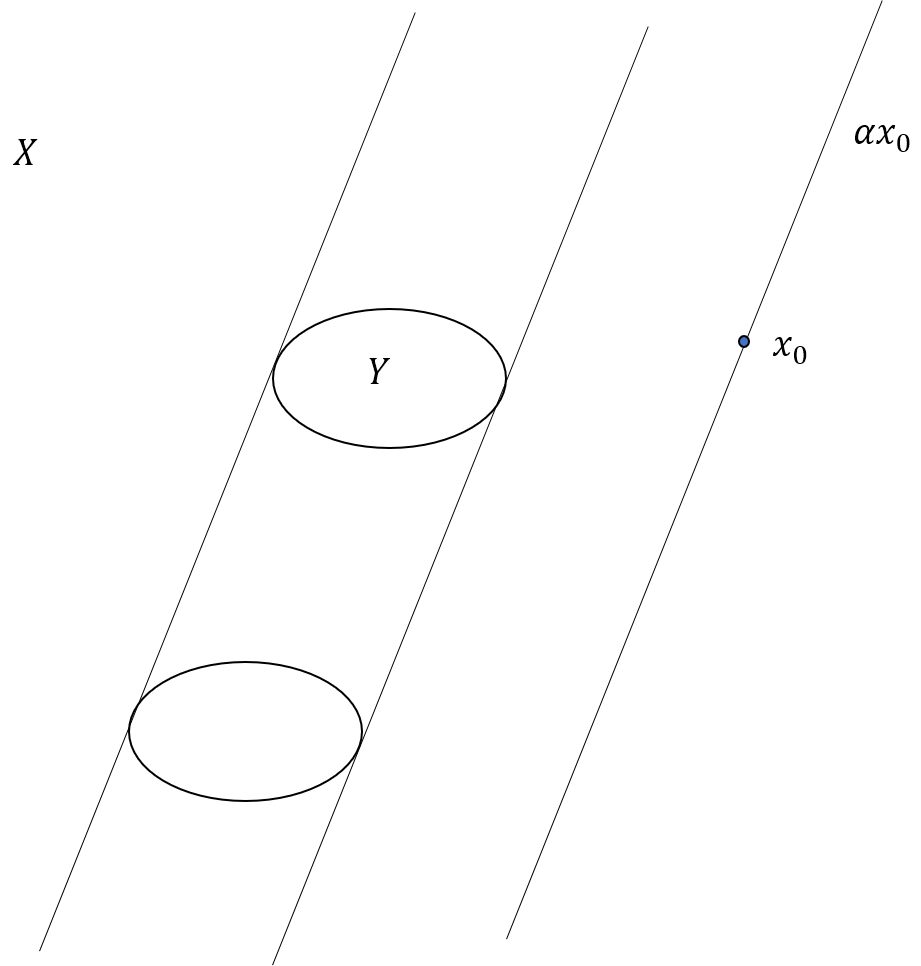
\includegraphics[width=0.5\linewidth]{figure/Domf.png}
\end{center}

(1)局部扩张的存在性.

(构造线性泛函$f\colon\Dom f\rightarrow\mathbb{R}$)现在证明存在线性泛函$f:U(x_0)\rightarrow\mathbb{R}$,它满足
\begin{empheq}{align*}
f(y)&=\ell (y),\forall y\in Y\\
f(x)&\leq p(x), \forall x\in\Dom f
\end{empheq}

假设$f$是存在的,那么它满足
\begin{empheq}{align*}
	f(\alpha x_0+y)&=\alpha f(x_0)+f(y)\\
	&=\alpha f(x_0)+\ell(y)\\
	&\leq p(\alpha x_0+y), \forall\alpha\in \mathbb{R},y\in Y
\end{empheq}

当$\alpha=0$时,显然是成立的(所以$f(y)=\ell(y),\forall y\in Y$自动成立).因为$f$是未知的,假如我们找到一个常数$\lambda\coloneqq f(x_0)$,即令
$$	f(\alpha x_0+y)=\alpha \lambda +\ell(y)$$

这就是一个线性泛函.需要它满足约束,因此现在来确定$\lambda$.
\begin{empheq}{align*}
&\alpha \lambda +\ell(y)\leq p(\alpha x_0+y)\\
\implies & \begin{aligned}[t]
	\lambda &\leq \frac{1}{\alpha}(p(\alpha x_0+y)-\ell y) ,\forall \alpha>0\\
	&=p\left(x_0+\frac{1}{\alpha}y\right)-\ell\left(\frac{1}{\alpha}y\right)
\end{aligned}
\end{empheq}

同时
\begin{empheq}{align*}
	&\alpha \lambda +\ell(y)\leq p(\alpha x_0+y)\\
	\implies & \begin{aligned}[t]
		\lambda &\geq \frac{1}{\alpha}(p(\alpha x_0+y)-\ell y) ,\forall \alpha<0\\
		&=\frac{1}{\alpha}\left(p\left(-\alpha\left(-x_0-\frac{1}{\alpha}y\right)\right)-\ell(y)\right)\\
		&=-p\left(-x_0-\frac{1}{\alpha}y\right)+\ell\left(-\frac{1}{\alpha}y\right)
	\end{aligned}
\end{empheq}

我们已经确定了$\lambda$潜在的上下界,现在还需要确定上界大于下界.由$\ell$的线性和$p$的次线性有
\begin{empheq}{align*}
\ell(u)+\ell(v) &=\ell(u+v),\forall u,v\in Y\\
\leq p(u+v)&=p(-x_0+u+x_0+v)\\
&\leq p(-x_0+u)+p(x_0+v)\\
\implies -p(x_0+u)+\ell(u)&\leq p(x_0+v)-\ell(v)
\end{empheq}

所以可以确定上界确实大于下界.那么取
\begin{empheq}{align*}
a\leq&\lambda\leq b\\
a&\coloneqq \sup_{u\in Y}\{-p(x_0+u)+\ell(u)\}\\
\leq b& \coloneqq \sup_{v\in Y}\{p(x_0+v)-\ell(v)\}
\end{empheq}

即可.

注意把$u,v$对应上去,实际上$u=-\frac{1}{\alpha}y$.

现在回头看思路,实际上构造的泛函是$h(x_0)=f(\alpha x_0+y)=\alpha \lambda +\ell(y)$,即对每个$x_0$有一个函数.反算回去,$\forall x\in U(x_0)$,它满足$f(x)\leq p(x)$.

(2)全局延拓的存在性.

(构造泛函集合)记$\mathcal{F}$为所有满足以下条件的泛函$f:\Dom f\rightarrow \mathbb{R}$的集合:
\begin{empheq}{align*}
f(y)&=\ell(y),\forall y\in Y\\
f(x)&\leq p(x),\forall y\in \Dom f
\end{empheq}

注意$y\subset \Dom f$,且$\Dom f$并非一个固定的子空间.

集合$\mathcal{F}$是非空的,因为$\ell\in \mathcal{F}$.此外,$\mathcal{F}$按以下关系$\preccurlyeq$是半序的:
$$f_1 \preccurlyeq f_2\iff \Dom f_1\subset \Dom f_2, f_2(x)=f_1(x),\forall x\in \Dom f_1$$

关系$\preccurlyeq$实际上就是延拓.

(证明全序子集有上界)给定一个$\mathcal{F}$的一个全序子集$\mathcal{E}$,令
$$\Dom g\coloneqq \bigcup_{f\in \mathcal{E}}\Dom f$$

它显然是$X$的子空间.以下证明,对于$\forall x\in \Dom g$,关系式
$$g(x)\coloneqq f(x), \forall x\in \Dom f, f\in \mathcal{E}$$

\circled{1}定义了一个线性泛函$g\colon \Dom g\rightarrow \mathbb{R}$,\circled{2}且$\forall x\in\Dom g,g(x)\leq p(x)$.

设$x\in \Dom g$使得$x\in \Dom f_1,x\in \Dom f_2$,而$f_1,f_2\in\mathcal{E}$,不妨设$f_1\preccurlyeq f_2$,因此
$$g(x)=f_1(x)=f_2(x)\leq p(x)$$

这证明了第二点.

又假如$x_1\in\Dom f_1,x_2\in\Dom f_2,f_1\preccurlyeq f_2$,那么$x_1+x_2\in\Dom f_2$(实际上$x_1$同时也属于$f_2$).因此$g(x_1+x_2)=f_2(x_1+x_2)=f_2(x_1)+f_2(x_2)=g(x_1)+g(x_2)$.同样地,$\forall \alpha \in \mathbb{R},g(\alpha x_1)=f_1(\alpha x_1)=\alpha f_1(x_1)=\alpha g(x_1)$.

这证明了第二点.

以上说明$g$是$\mathcal{E}$的上界.这是因为$\forall f\in \mathcal{E},\Dom f\subset \Dom g$.

(选择极大元)由Zorn引理,集合$\mathcal{F}$有极大元$\widetilde{\ell}$,它定义在子空间$\Dom \widetilde{\ell}$上.然后有
$$\Dom \widetilde{\ell}=X$$

这就是说$\widetilde{\ell}$正是我们想要找到的泛函.如果$\Dom \widetilde{\ell}\subsetneqq X$,那么可以像第(1)部分一样继续扩张,构造泛函$\widetilde{f}\colon \Dom \widetilde{f}\rightarrow \mathbb{R}$,它满足
$$\Dom \widetilde{\ell}\subsetneqq \Dom \widetilde{f},\widetilde{f}(y)=\ell(y),\forall y\in Y$$
$$\widetilde{f}\leq p(x),\forall x\in \Dom \widetilde{f}$$

这说明$\widetilde{\ell}$不是极大元,矛盾.

因此原命题得证.

\end{proof}

在这个证明中,我们首先进行局部延拓,再通过选择极大元延拓到全局.



\chapter{微分几何与张量分析}
这一章节从两个角度来写.第一是形象的微分几何,比如曲线理论、曲面理论.第二是抽象的微分几何,比如流形理论.

\section{曲线理论}
\subsection{曲线的表示}
曲线有平面与空间曲线,后者一般可以从前者扩展面来.

\subsubsection{参数表示法}
\begin{empheq}[left=\empheqlbrace]{align*}
x&=x(t)\\
y&=y(t)
\end{empheq}
也可以用向量来表示
$$\bm{r}=\bm{r}(t)$$

\subsubsection{隐式表示}
用方程表示
$$F(x,y)=0$$

\subsubsection{弧长表示}
将曲线坐标表示为弧长的函数
$$\bm{r}=\bm{r}(s)$$

这种表示法比较难算,因为弧长是积分.但后面可以看到,弧长表示法易于表达曲率、挠率等概念.

以下用$t$表示一般参数表达,用$s$表示弧长表达.

\subsection{与曲线有关的量}
\subsubsection{弧长}
\begin{empheq}{align*}
s&=\int_{a}^{b} \sqrt{x'(t)^2+y'(t)^2}\dif t \mtag{平面曲线}\\
&=\int_{a}^{b} \sqrt{x'(t)^2+y'(t)^2+z'(t)^2}\dif t \mtag{空间曲线}\\
&=\int_{a}^{b} |\bm{r}'(t)| \dif t
\end{empheq}

\subsubsection{切向量}
就是梯度$\bm{t}=\bm{r}'(s)$.
\subsubsection{曲率}
与二阶导数有关.
\begin{empheq}{align*}
k&=\frac{x'y''-y'x''}{(x'^2+y'^2)^{\frac{3}{2}}} \mtag{平面曲线}\\
&=|\bm{r}''(s)|\\
R&=\frac{1}{|k|} \mtag{曲率半径}
\end{empheq}

\subsubsection{单位法向量}
$$\bm{n}=\frac{1}{k}\bm{r}''(s)$$
\subsubsection{副法向量}
$$\bm{b}=\bm{t}\bm{n}$$
\subsubsection{挠率}
三阶导数.

\subsubsection{奇点}
即导数为0的点,即$\bm{r}'(t)=0$.

\subsection{各种平面曲线}
\subsubsection{椭圆}

\subsection{各种空间曲线}

\section{曲面理论}
\subsection{曲面的表示}
\subsubsection{第一基本型}
给定曲面$\bm{r}(u,v)$,$\bm{r}$是三维向量。则第一基本型的系数为$E,F,G$,则线元素为
$$I=E\dif u^2+2F\dif u\dif v+G\dif v^2$$
其中
\begin{empheq}{align*}
E&=\bm{r}_u\cdot \bm{r}_u\\
F&=\bm{r}_u\cdot \bm{r}_v\\
G&=\bm{r}_v\cdot \bm{r}_v
\end{empheq}
所谓线元素是指线段$\bm{r}(u,v)$到$\bm{r}(u+\dif u,v+\dif v)$的长度。

从形式上看,第一基本型与度量张量\eqref{metric-tensor}的表示一模一样。其实
\begin{empheq}[left=\empheqlbrace]{align*}
E&=g_{11}\\
F&=g_{12}=g_{21}\\
G&=g_{22}
\end{empheq}

可以看出,曲面相当于$R^2\rightarrow R^3$的映射,而一般的坐标变换是$R^n\rightarrow R^n$的映射,在两种情况下都可以计算度规。

面积元为
$$\dif A=|\bm{r}_u\times \bm{r}_v|\dif u\dif v=\sqrt{|g|}\dif u\dif v$$

\subsubsection{第二基本型}
给定曲面$\bm{r}=\bm{r}(u,v)$
$$II = L\dif u^2 + 2M \dif u\dif v+N\dif v^2$$
其中
\begin{empheq}{align*}
\bm{n}&=\frac{\bm{r}_u\times \bm{r}_v}{|\bm{r}_u\times \bm{r}_v|}\\
L&=\bm{r}_{uu}\cdot \bm{n}\\
M&=\bm{r}_{uv}\cdot \bm{n}\\
N&=\bm{r}_{vv}\cdot \bm{n}
\end{empheq}

第二基本型的实质是邻近点到切平面的有向距离。对于一个点$\bm{r}(u_0,v_0)$,该点处法向量为$\bm{n}$,取切平面$\pi$,再取一个邻近点$\bm{r}(u+\Delta u,v+\Delta v)$,则点到$\pi$的有向距离是
$$\delta(\Delta u,\Delta v)=(\bm{r}(u+\Delta u,v+\Delta v)-\bm{r}(u,v))\cdot\bm{n}=\frac{1}{2}II+o(\Delta^2 u+\Delta^2 v)$$

显然,第二基本型可以用来表示曲面的弯曲程度,某点处的值越大,表示微扰带来的偏离越远,则弯曲得越厉害。

\subsubsection{作为曲面的3D函数}
考虑一个3D函数$f(x,y)$,取曲面$\bm{r}(u,v,f(u,v))$。则
\begin{empheq}{align*}
\bm{r}_u&=(1,0,f_u)\\
\bm{r}_v&=(0,1,f_v)\\
\bm{n}&=\frac{(-f_u,-f_v,1)}{\sqrt{f_u^2+f_v^2+1}}\\
\bm{r}_{uu}&=(0,0,f_{uu})\\
\bm{r}_{uv}&=(0,0,f_{uv})\\
\bm{r}_{vv}&=(0,0,f_{vv})\\
J&=\begin{bmatrix}
\bm{r}_u&\bm{r}_v
\end{bmatrix}\\
G_{ij}&=J^TJ=\begin{bmatrix}
1+(f_u)^2&f_uf_v\\
f_vf_u&1+(f_v)^2
\end{bmatrix}\\
G^{ij}&=G_{ij}^{-1}=\inv{(f_u)^2+(f_v)^2+1}\begin{bmatrix}
1+(f_v)^2&-f_uf_v\\
-f_uf_v&1+(f_u)^2
\end{bmatrix}
\end{empheq}

Christoffel符号有8个:$1\leq i,j,k\leq 2$。
\subsection{曲面的性质}
\subsubsection{测地线}
测地线是测地曲率为0的点,是直线概念的推广,但在任意维的流形上,测地线不一定是最短的,不过最短的一定是测地线。也就是说测地线可能不惟一。

在黎曼度量下,对于三维曲面,其含义是
\begin{empheq}[box=\fbox]{equation}
\frac{D}{\dif  t}\left(\odv{\bm{r}(u(t),v(t))}{t}\right)
\end{empheq}

任意维的度量中,测地线按以下方程组给出:
\begin{empheq}[box=\fbox]{equation}
\pdv[order={2}]{u^i}{t}+\Gamma^i_{jk}\pdv{u^j}{t}\pdv{u^k}{t}=0,1\leq i\leq n
\end{empheq}
注意这里$u,v$实际上是单参数函数。

初始条件可以按两种方式给出,一是边值问题,即给定起点$[u(0),v(0)]$与终点$[u(1),v(1)]$。二是初值问题,给定起点$[u(0),v(0)]$与方向$[u'(0),v'(0)]$。对于三维曲面$f(u,v)$,测地线由参数方程$[u[t],v[t],f(u[t],v[t])]$给出。

但是黎曼度量在代数曲面上可能难以计算,所以还是从测地曲率的角度考虑比较好。

\section{超曲面}
\subsection{超曲面上的几何}
\subsubsection{切丛}
给定一个$n$元函数$F(\bx)$,其在某点$\bm{p}_0$处的梯度为$\nabla F(\bm{p}_0)$,等值面为$F(\bx)=F(\bm{p}_0)$,维度是$n-1$,等值面的法向量为$\nabla F(\bm{p}_0)$(法向量是梯度),$tF(\bm{p}_0)$为法向量空间,其维度是$1$,等值面在该点处的切空间为$\nabla F(\bm{p}_0)\cdot \bx-\nabla F(\bm{p}_0)\cdot\bm{p}_0=0$(切空间过点,且垂直于梯度)。所以说某点等值面的法向量就是函数的梯度。

另一方面,$n$元函数可以视为一个$n+1$维平面$F(\bx)-x_{n+1}=0$,该点处的切空间为
$$\begin{bmatrix}
\nabla F(\bm{p}_0) & -1
\end{bmatrix}\cdot \begin{bmatrix}
\bx & x_{n+1}
\end{bmatrix}=\begin{bmatrix}
\nabla F(\bm{p}_0) & -1
\end{bmatrix}\cdot \begin{bmatrix}
\bm{p}_0 & F(\bm{p}_0)
\end{bmatrix}$$
或者
\begin{empheq}{align*}
x_{n+1}&=\nabla F(\bm{p}_0)\cdot \bx-(\nabla F(\bm{p}_0)\cdot \bm{p}_0-F(\bm{p}_0))\\
&=F(\bm{p}_0)+\nabla F(\bm{p}_0) \cdot ( \bx-\bm{p}_0)
\end{empheq}
注意,这里其实就是一阶泰勒展开,所以切平面相当于一阶泰勒展开式。注意第一项是偏移量,第二项是等值面的切空间。
\subsection{曲面理论定理}
\section{张量与场}
\subsection{度规与联络}\label{tensor-field-metric}
度规(或者度量张量)的含义是:
\begin{empheq}[box=\fbox]{equation}
\dif s^2=g_{ij}\dif x^i \dif x^j\label{metric-tensor}
\end{empheq}

对于曲面坐标系中的张量,有:
\begin{empheq}[box=\fbox]{align}
A_i&=g_{ik}A^k
\end{empheq}

给定坐标系$x_i=x_i(x^i,x^j,x^k)$,$x_i$是欧几里得坐标(一般用下标表示),则
\begin{empheq}{align}
g_{ij}&=\sum_{i=1}^{3}\pdv{x_k}{x^i}\pdv{x_k}{x^j}\\
g^{ij}&=\sum_{i=1}^{3}\pdv{x^i}{x^k}\pdv{x^j}{x^k}
\end{empheq}
注意,$g_{ij}$和$g^{ij}$通常是$x^i$的函数,即曲线坐标。它也可以用矩阵形式表示:
\begin{empheq}{align}
(g_{ij})=J^TJ=G\\
(g^{ij})=G^{-1}
\end{empheq}
$J$为Jacobi矩阵:
\[J=\pdv{{(x_1,x_2,x_3)}}{{(x^1,x^2,x^3)}}=\begin{bmatrix}
\pdv{x_1}{x^1} &\pdv{x_1}{x^2}&\pdv{x_1}{x^3}\\
\pdv{x_2}{x^1} &\pdv{x_2}{x^2}&\pdv{x_2}{x^3}\\
\pdv{x_3}{x^1} &\pdv{x_3}{x^2}&\pdv{x_3}{x^3}
\end{bmatrix}\]


度规的导数与协变导数按下式给出:
\begin{empheq}{align*}
	\pdv{g^{ik}}{x^l}&=-\Gamma^i_{ml}g^{mk}-\Gamma^k_{ml}g^{im}\\
	g^{ik}_{;l}&=g_{ik;l}=0
\end{empheq}

\subsection{Christoffel符号}
\begin{empheq}[box=\fbox]{align}
\Gamma_{i,kl}&=\frac{1}{2}\left(\pdv{g_{ik}}{x^l}+\pdv{g_{il}}{x^k}-\pdv{g_{kl}}{x^i}\right)\\
\Gamma^i_{jk}&=\frac{1}{2}g^{im}\left(\pdv{g_{mk}}{x^l}+\pdv{g_{ml}}{x^k}-\pdv{g_{kl}}{x^m}\right)=g^{im}\Gamma_{m,kl}
\end{empheq}

\subsection{协变导数}
张量的协变导数定义为
\begin{empheq}[box=\fbox]{align}
DA_i&=g_{ik}DA^k\label{DA_ig}\\
	DA^{ik}&=\dif A^{ik}-\delta A^{ik}\equiv A^{ik}_{;l}\dif x^l\mtag{协变微分}\\
A^{ik}_{;l}&=\pdv{A^{ik}}{x^l}+\Gamma^i_{ml}A^{mk}+\Gamma^k_{ml}A^{im}\\
A^i_{k;l}&=\pdv{A^i_k}{x^l}-\Gamma^m_{kl}A^i_m+\Gamma^i_{ml}A^m_k\\
A_{ik;l}&=\pdv{A_{ik}}{x^l}-\Gamma^m_{il}A_{mk}+\Gamma^m_{kl}A_{im}
\end{empheq}

协变微分可以按如下方式理解。
\begin{center}
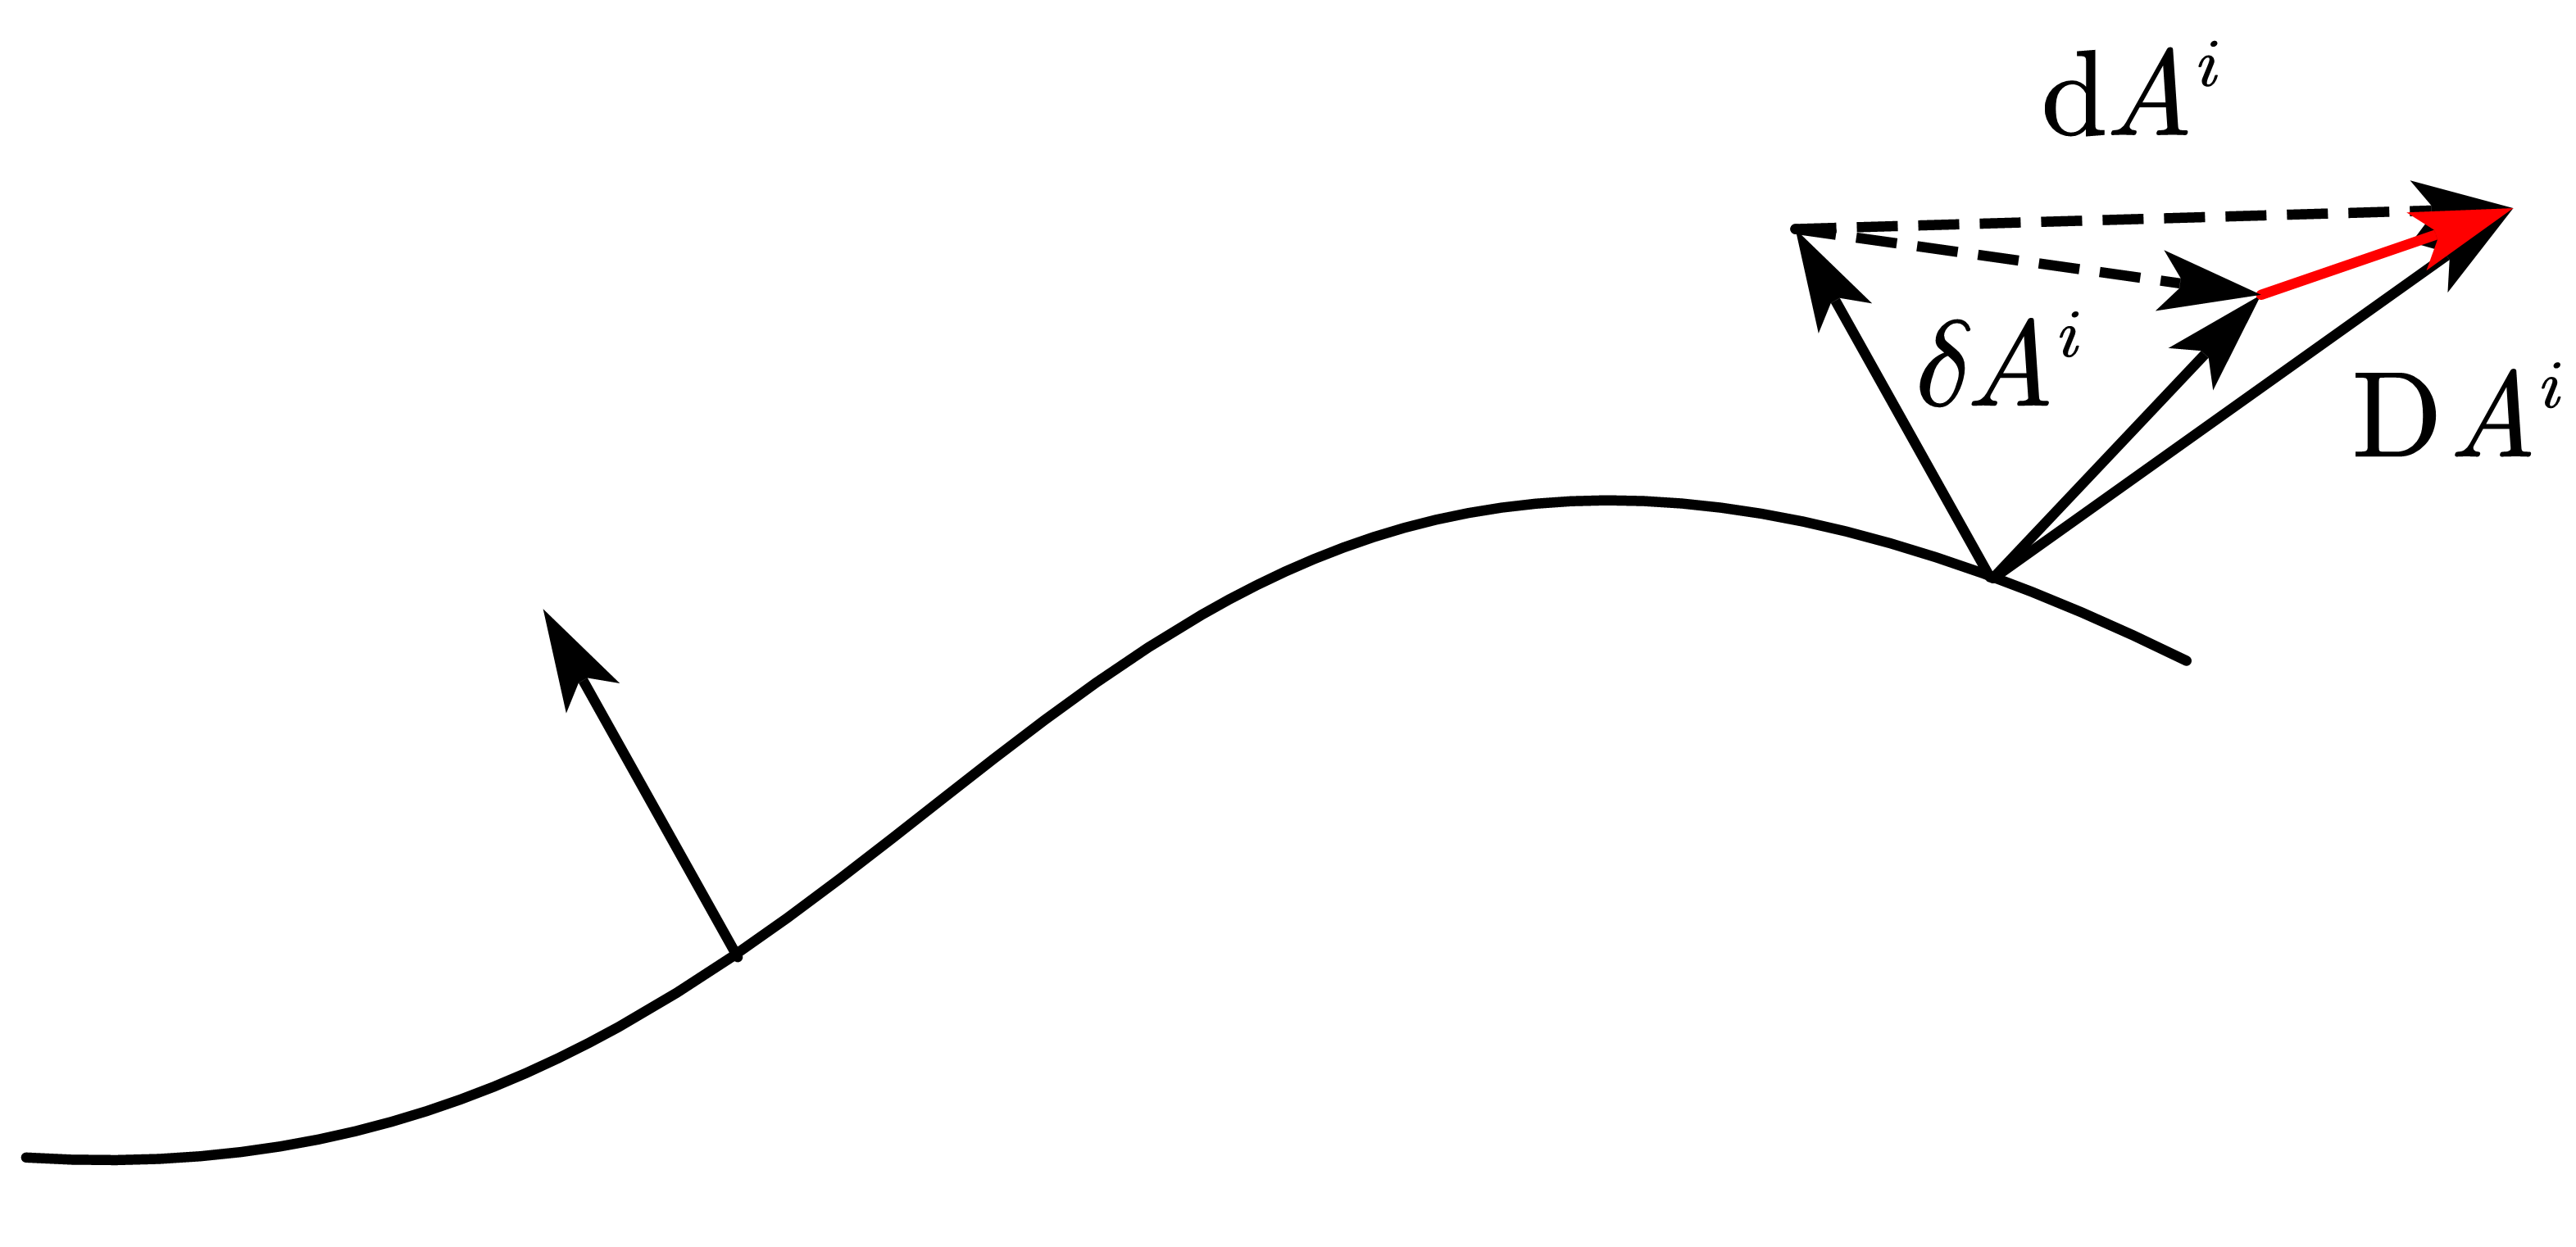
\includegraphics[width=8cm]{figure/CovariantDifferential.png}
\end{center}

我们希望计算微小坐标变化下引起的矢量的变动。如果直接把两个矢量相减,得到的是$\dif A^i$。但空间是弯曲的,假如把一个矢量沿着空间“平行移动”到与另一个矢量同起点,相对于之前的矢量,发生的变化是$\delta A^i$。协变微分就是图中的红线,即将一个矢量平行移动后计算的微分(如果两个矢量不是同起点,不能直接相减)。
\subsection{曲率}
\begin{empheq}[box=\fbox]{align}
R^i_{klm}&=\pdv{\Gamma^i_{km}}{x^l}-\pdv{\Gamma^i_{kl}}{x^m}+\Gamma^i_{nl}\Gamma_{km}^n-\Gamma_{nm}^i\Gamma_{kl}^n\mtag{黎曼曲率张量}\\
R_{iklm}&=g_{in}R^n_{klm}\\
R_{ik}&=g^{lm}R_{limk}=R^l_{ilk\cdot}\mtag{Ricci张量}\\
R&=g^{ik}R_{ik}=g^{il}g^{km}R_{iklm}\mtag{曲率标量}
\end{empheq}

\paragraph*{曲率张量的性质}以下前两个式子是说它关于$ik$和$lm$的第一对是反对称的。
\begin{empheq}{align}
R_{iklm}&=-R_{kilm}=-R_{ikml}\nonumber\\
R_{iklm}&=R_{lmik}\nonumber\\
R_{iklm}+R_{imkl}+R_{ilmk}&=0\nonumber\\
R^k_{ijl}+R^k_{jli}+R^k_{lij}&=0\mtag{第一比安基恒等式}\\
R^k_{ijl;h}+R^k_{ilh;j}+R^k_{ihj;l}&=0\mtag{第二比安基恒等式}
\end{empheq}
\section{空间坐标系}
\subsection{极坐标}\label{polar-coord}
\begin{center}
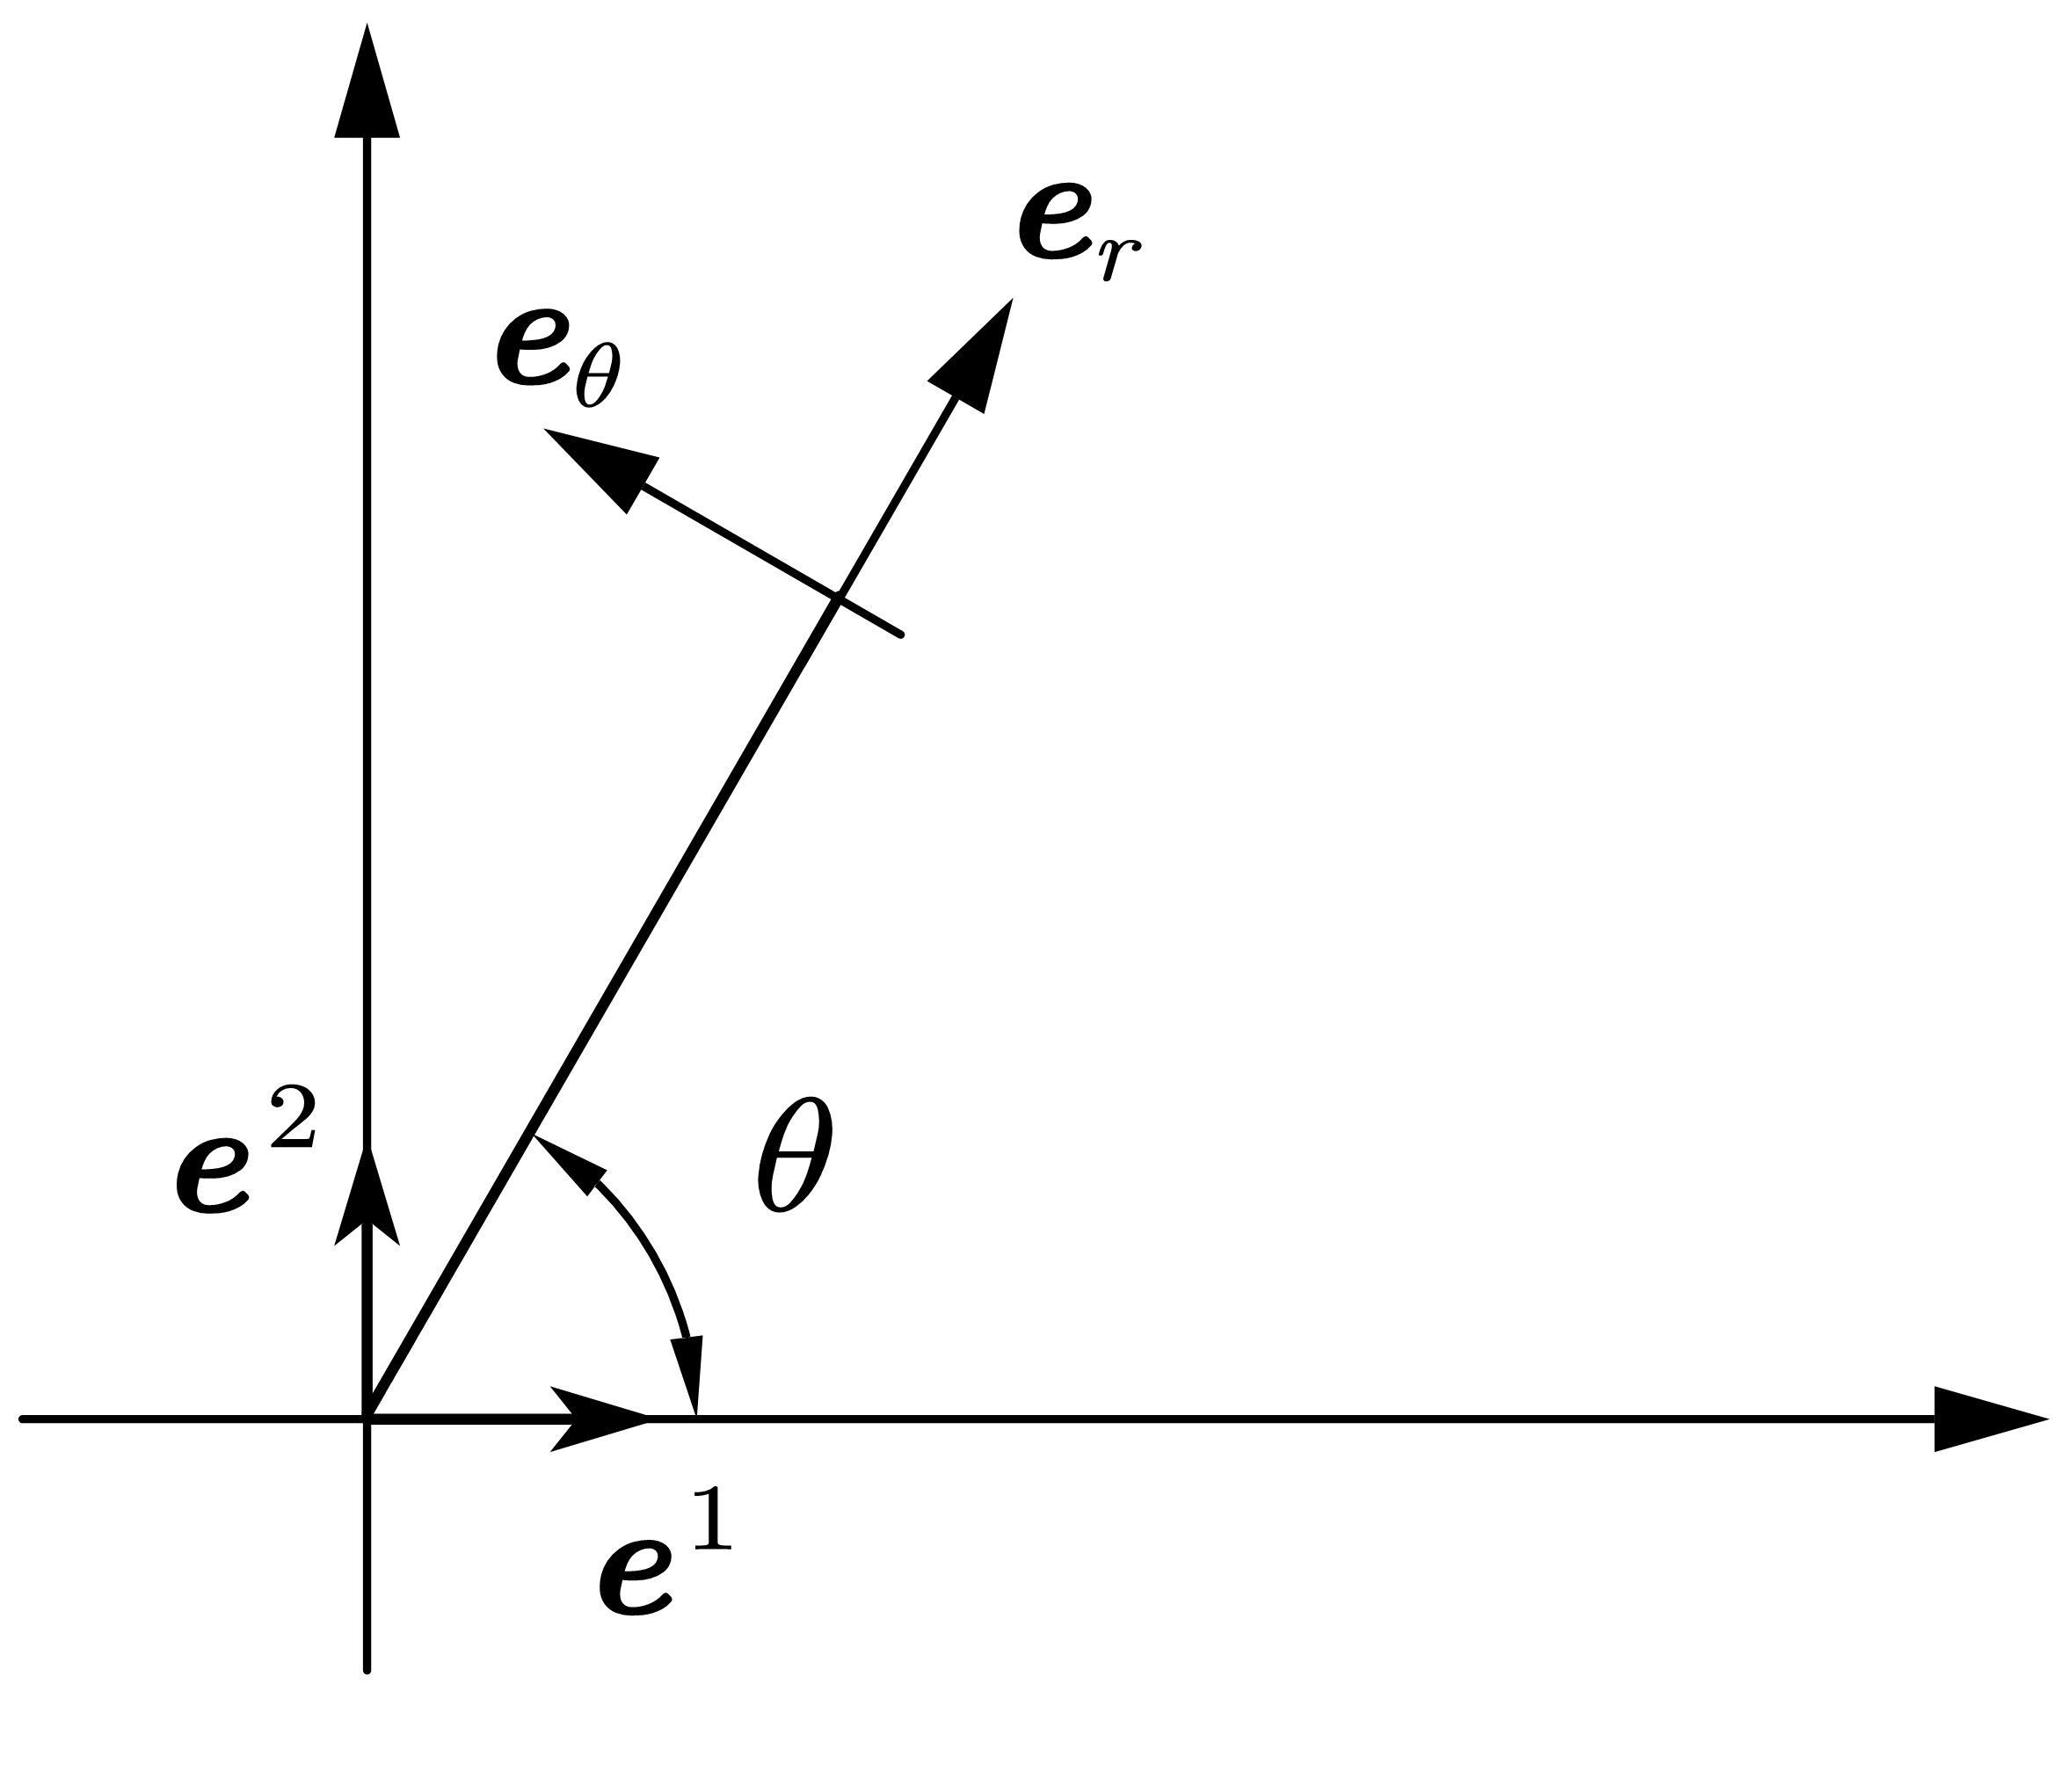
\includegraphics[width=5cm]{figure/polar-coord.png}
\end{center}

\begin{empheq}[left=\empheqlbrace]{align*}
x&=r\cos\theta\\
y&=r\sin\theta
\end{empheq}
求解
\[
(g_{ij})=\begin{bmatrix}
g_{rr} & g_{r\theta}\\
g_{\theta r}&g_{\theta\theta}
\end{bmatrix}=\begin{bmatrix}
1&0\\
0& r^2
\end{bmatrix}
,\quad (g^{ij})=(g_{ij})^{-1}\begin{bmatrix}
	1&0\\
	0& \frac{1}{r^2}
\end{bmatrix}\]
从度量中可以看出,极坐标系是正交坐标系。另外有基变换
\begin{empheq}{align*}
\bm{e}_r&=\pdv{x_i}{r}\bm{e}^i=\cos\theta\bm{e}^1+\sin\theta \bm{e}^2\\
\bm{e}_\theta&=\pdv{x_i}{\theta}\bm{e}^i=-r\sin\theta\bm{e}^1+r\cos\theta\bm{e}^2
\end{empheq}
\subsection{柱坐标}

\subsection{球坐标}
\subsubsection{坐标表示}
这里使用物理学中的约定。

\begin{center}
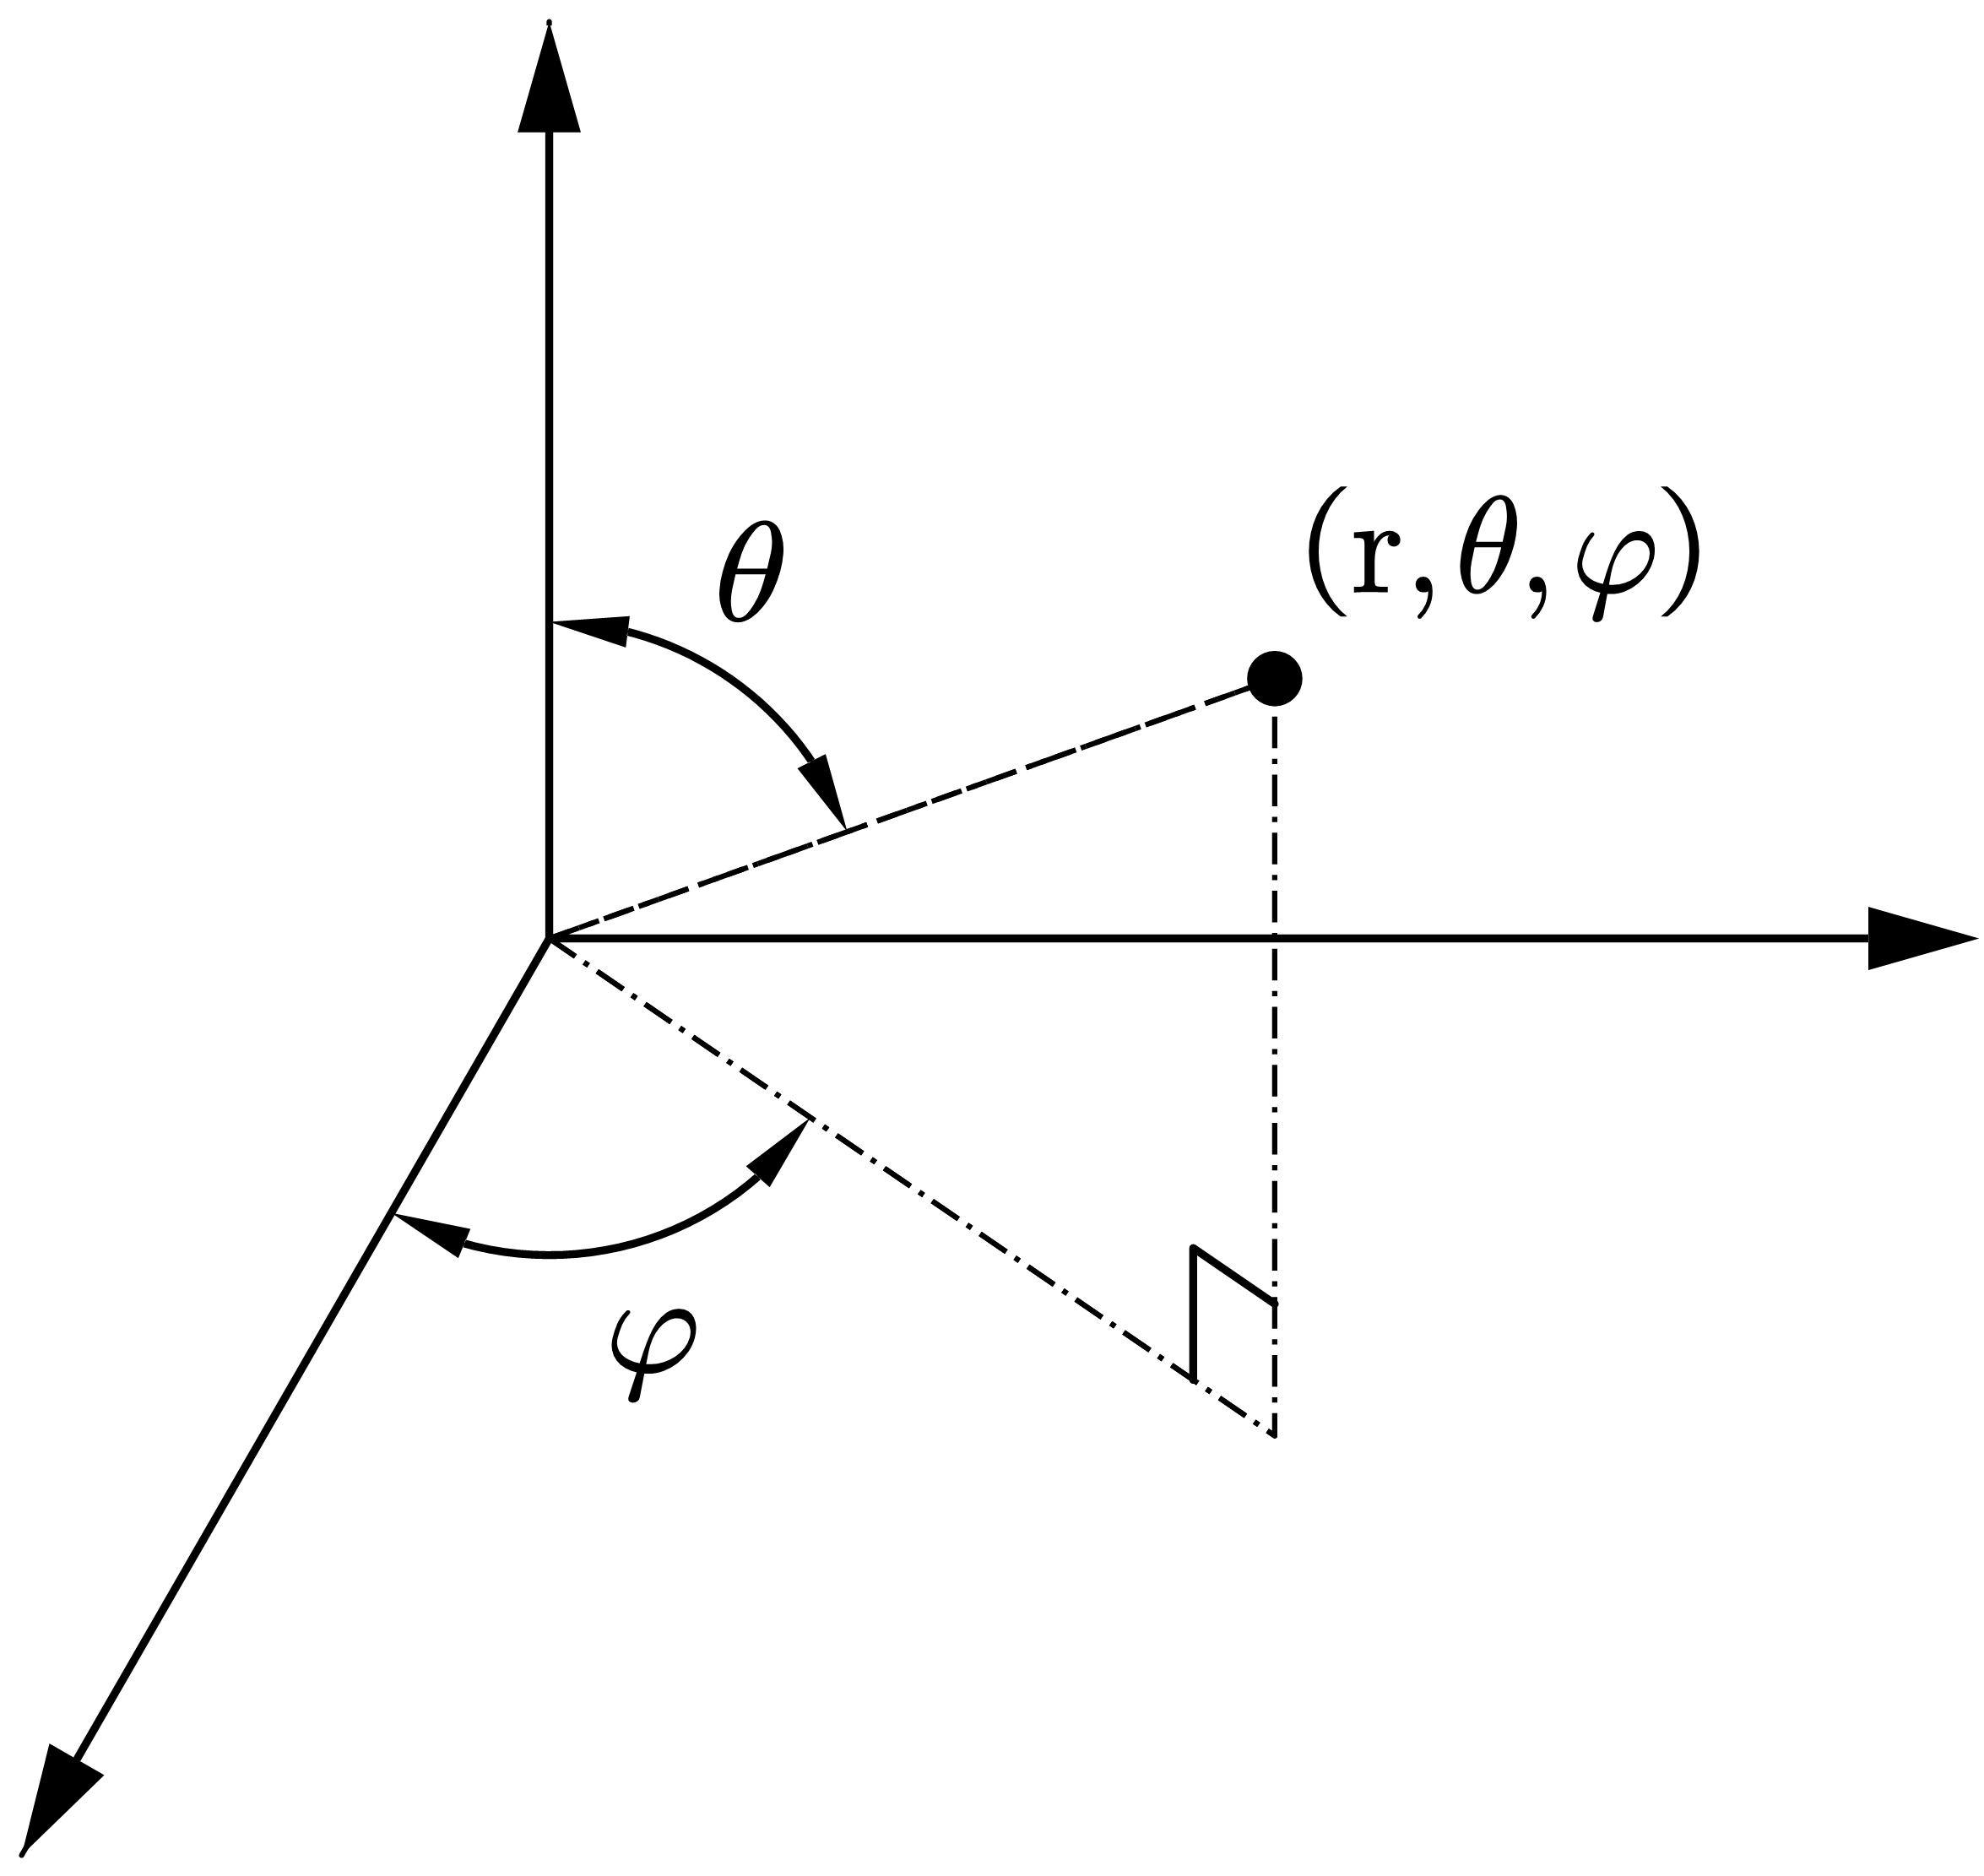
\includegraphics[width=4cm]{figure/Sphere3D.png}
\end{center}
\begin{empheq}[left=\empheqlbrace]{align}
x&=r\sin\theta\cos\phi\\
y&=r\sin\theta\sin\phi\\
z&=r\cos\theta
\end{empheq}

\subsubsection{微分公式}
\begin{center}
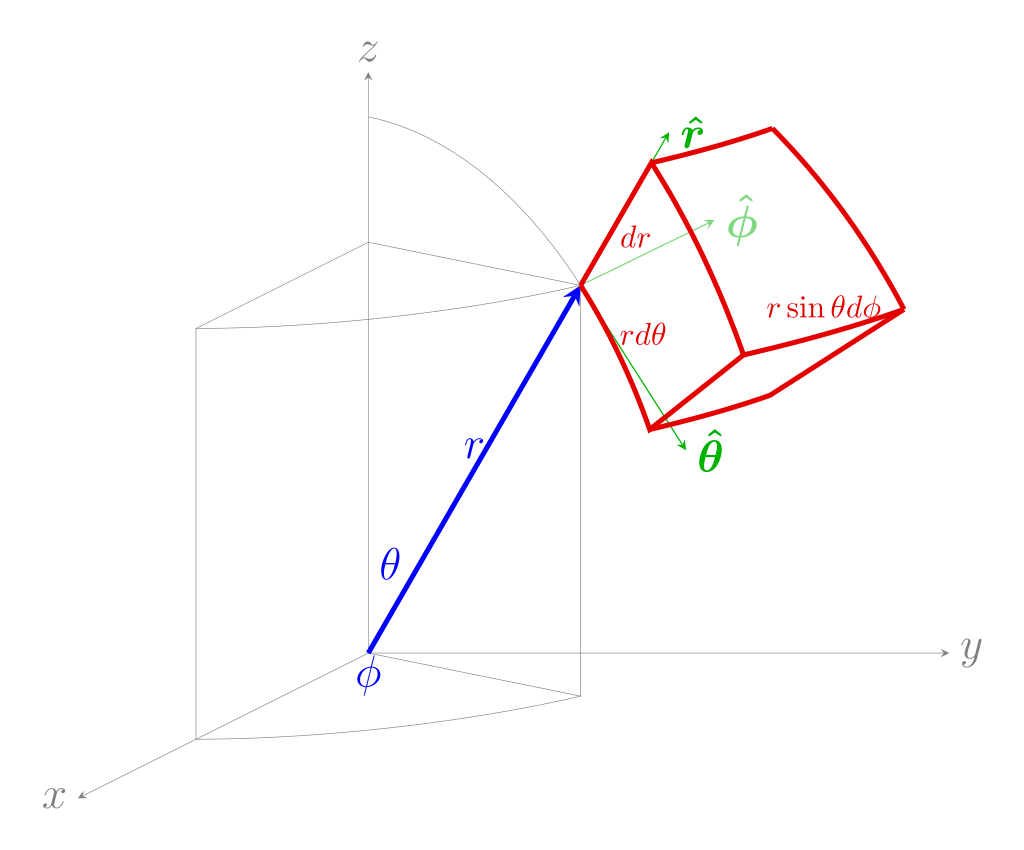
\includegraphics[width=6cm]{figure/Sphere3DDiff.png}
\end{center}

\begin{description}
\item[线元素] 从$(r,\theta,\varphi)$到$(r+\dif r,\theta+\dif \theta,\varphi+\dif \varphi)$的无穷小位移,表示为
$$\dif \bm{r}=\dif r \hat{\bm{r}}+r\dif\theta\hat{\bm{\theta}}+r\sin\theta\dif\varphi\hat{\bm{\varphi}}$$
$\hat{\bm{r}},\hat{\bm{\theta}},\hat{\bm{\varphi}}$为单位矢量。
\item[体积元素] $$\dif V=r^2\sin\theta\dif r\dif\theta\dif\varphi$$
\item[梯度公式] $$\nabla f=\frac{\partial f}{\partial r}\hat{\bm{r}}+\frac{1}{r}\frac{\partial f}{\partial \theta}\hat{\bm{\theta}}+\frac{1}{r\sin\theta}\frac{\partial f}{\partial \varphi}\hat{\bm{\varphi}}$$
\item[拉普拉斯算子] $$\nabla^2f=\frac{1}{r^2}\frac{\partial}{\partial r}\left(r^2\frac{\partial f}{\partial r}\right)+\frac{1}{r^2\sin\theta}\frac{\partial }{\partial\theta}\left(\sin\theta\frac{\partial f}{\partial \theta}\right)+\frac{1}{r^2\sin^2\theta}\frac{\partial^2f}{\partial \varphi^2}$$
\end{description}


\section{微分形式}

\chapter{拓扑与流形}
\section{Riemann流形}

\section{Teichmuller空间}

\chapter{模形式}
\chapter{变分法}\label{variant-of-calculus}

\section{变分法原理}
\subsection{变分的定义}
\subsubsection{积分的变分}
\paragraph*{一元积分}$x$为自变量,$y(x)$为一个光滑函数,取$\varepsilon$为一极小量,$\eta(x)$为一光滑函数。积分
$$I(y)=\int_a^b F(x,y(x),y'(x))\dif x$$
则定义
\begin{empheq}{align}
I(y+\delta\eta)-I(y)&=\int_a^b F(x,y+\delta\eta,(y+\delta\eta)')-F(x,y,y')\dif x\\
&=\int_a^b \left[\left(\delta y\pdv{}{y}+(\delta y)'\pdv{}{y'}\right)F+\inv{2}\left(\delta y\pdv{}{y}+(\delta y)'\pdv{}{y'}\right)^2F+\cdots\right]\dif x\\
&=\delta I(y)+\inv{2}\delta^2I(y)+\cdots
\end{empheq}

于是可以看出:
\begin{empheq}{align}
\delta I(y)&=\int_a^b \left(\delta y\pdv{}{y}+(\delta y)'\pdv{}{y'}\right)F\dif x\\
&=\int_a^b \delta y\pdv{F}{y}\dif x+\left.\delta y\pdv{F}{y'}\right|_a^b-\int_a^b \delta y\odv{}{x}\pdv{F}{y}\dif x\\
&=\int_a^b \left(\pdv{F}{y}-\odv{}{x}\pdv{F}{y'}\right)\delta y\dif x
\end{empheq}
这里用了分部积分。

从以上可以看出,所谓变分,就是在一个光滑函数的微小扰动下积分的改变量。

\paragraph*{一阶最优条件}问题
$$\min_y I(y)$$
的一阶条件就是
\begin{empheq}{equation}\label{1d-varition-min-1st-order-cond}
\delta I(y)=0\implies \pdv{F}{y}-\odv{}{x}\pdv{F}{y'}=0
\end{empheq}

有的地方也这样定义变分:
\begin{empheq}{align}
\delta_1 I(y,\eta)&=\left.\odv{I(y+\varepsilon \eta)}{\varepsilon}\right|_{\varepsilon=0}\\
&=\int_a^b \left(\pdv{F}{y}-\odv{}{x}\pdv{F}{y'}\right)\dif x\\
&=\frac{\delta I}{\delta}
\end{empheq}
这个定义与前面的实质相同。叫做Gateaux变分,是方向导数的推广。物理学中前一种用的多,Gateaux用的不多。

\paragraph*{一阶最优条件的特殊情形}

\begin{description}
\item[不显含$x$] 函数为$F(y,y')$。取
\begin{empheq}{align}
\odv{}{x}\left(y'\pdv{F}{y'}-F\right)&=y''\pdv{F}{y'}+y'\odv{}{x}\pdv{F}{y'}-\left(\pdv{F}{y}y'+\pdv{F}{y'}y''\right)\\
&=-y'\left(\pdv{F}{y}-\odv{}{x}\pdv{F}{y'}\right)\\
\implies &F-y'\pdv{F}{y'}=\text{const} \label{1d-varition-min-1st-order-cond-special-1}
\end{empheq}
\item[不显含$y$] 函数为$F(x,y')$,直接代入有:
\begin{empheq}{equation}\label{1d-varition-min-1st-order-cond-special-2}
\pdv{F}{y'}=\text{const}
\end{empheq}
\item[不显含$y'$] 函数为$F(x,y)$。 直接代入\cref{1d-varition-min-1st-order-cond}即得:
\begin{empheq}{equation}\label{1d-varition-min-1st-order-cond-special-3}
\pdv{F}{y}=0
\end{empheq}

\end{description}

\paragraph*{一元变分与偏微分记号}假如$F$函数不显含$y'$,则有
\begin{empheq}{align}
\delta I=\int_a^b \varepsilon y\pdv{F}{y}\dif x
\end{empheq}
则可以记
$$\frac{\delta I}{\varepsilon y}=\pdv{I}{y}=\pdv{F}{y}$$
一阶条件\cref{1d-varition-min-1st-order-cond}现在就是
$$\pdv{F}{y}=0$$
这里的偏微分只是一种记号,不要把它与一般的微分混淆。$\pdv{F}{y}$是$x$的函数,但是$I$本身是一个积分,不是$x$的函数。
\paragraph*{多元积分}考虑一个更一般的多元积分:
$$I(y)=\int_{\Omega}F(\bx, y(\bx),\nabla y(\bx))\dif V$$
$\bx\in\Rns$,$y$仍是标量函数,此时
\begin{empheq}{align}
\delta I(y)&=\int_{\Omega} \left(\pdv{L}{y}-\sum_k \pdv{}{x_k}\pdv{F}{y_k'}\right)\delta y\dif V
\end{empheq}
这里$u_k'=\pdv{y}{x_k}$。
\subsubsection{变分运算的法则}
\begin{enumerate}
\item 与微分交换:
$$(\delta y)'=\delta y'$$
\item 与积分交换:
$$\delta \int_a^b F\dif x=\int_a^b \delta F\dif x$$
\item 复合函数的变分与微分相同:
$$\delta F(x,y,y')=F_2\delta y+F_3\delta y'$$
\end{enumerate}
\subsection{约束变分与拉格朗日法}

\section{变分法的应用}

\subsection{几何优化}

\subsection{运动学}
\subsubsection{最速降线}
\paragraph*{曲线方程}
\begin{example}
建立如下坐标系:
\begin{center}
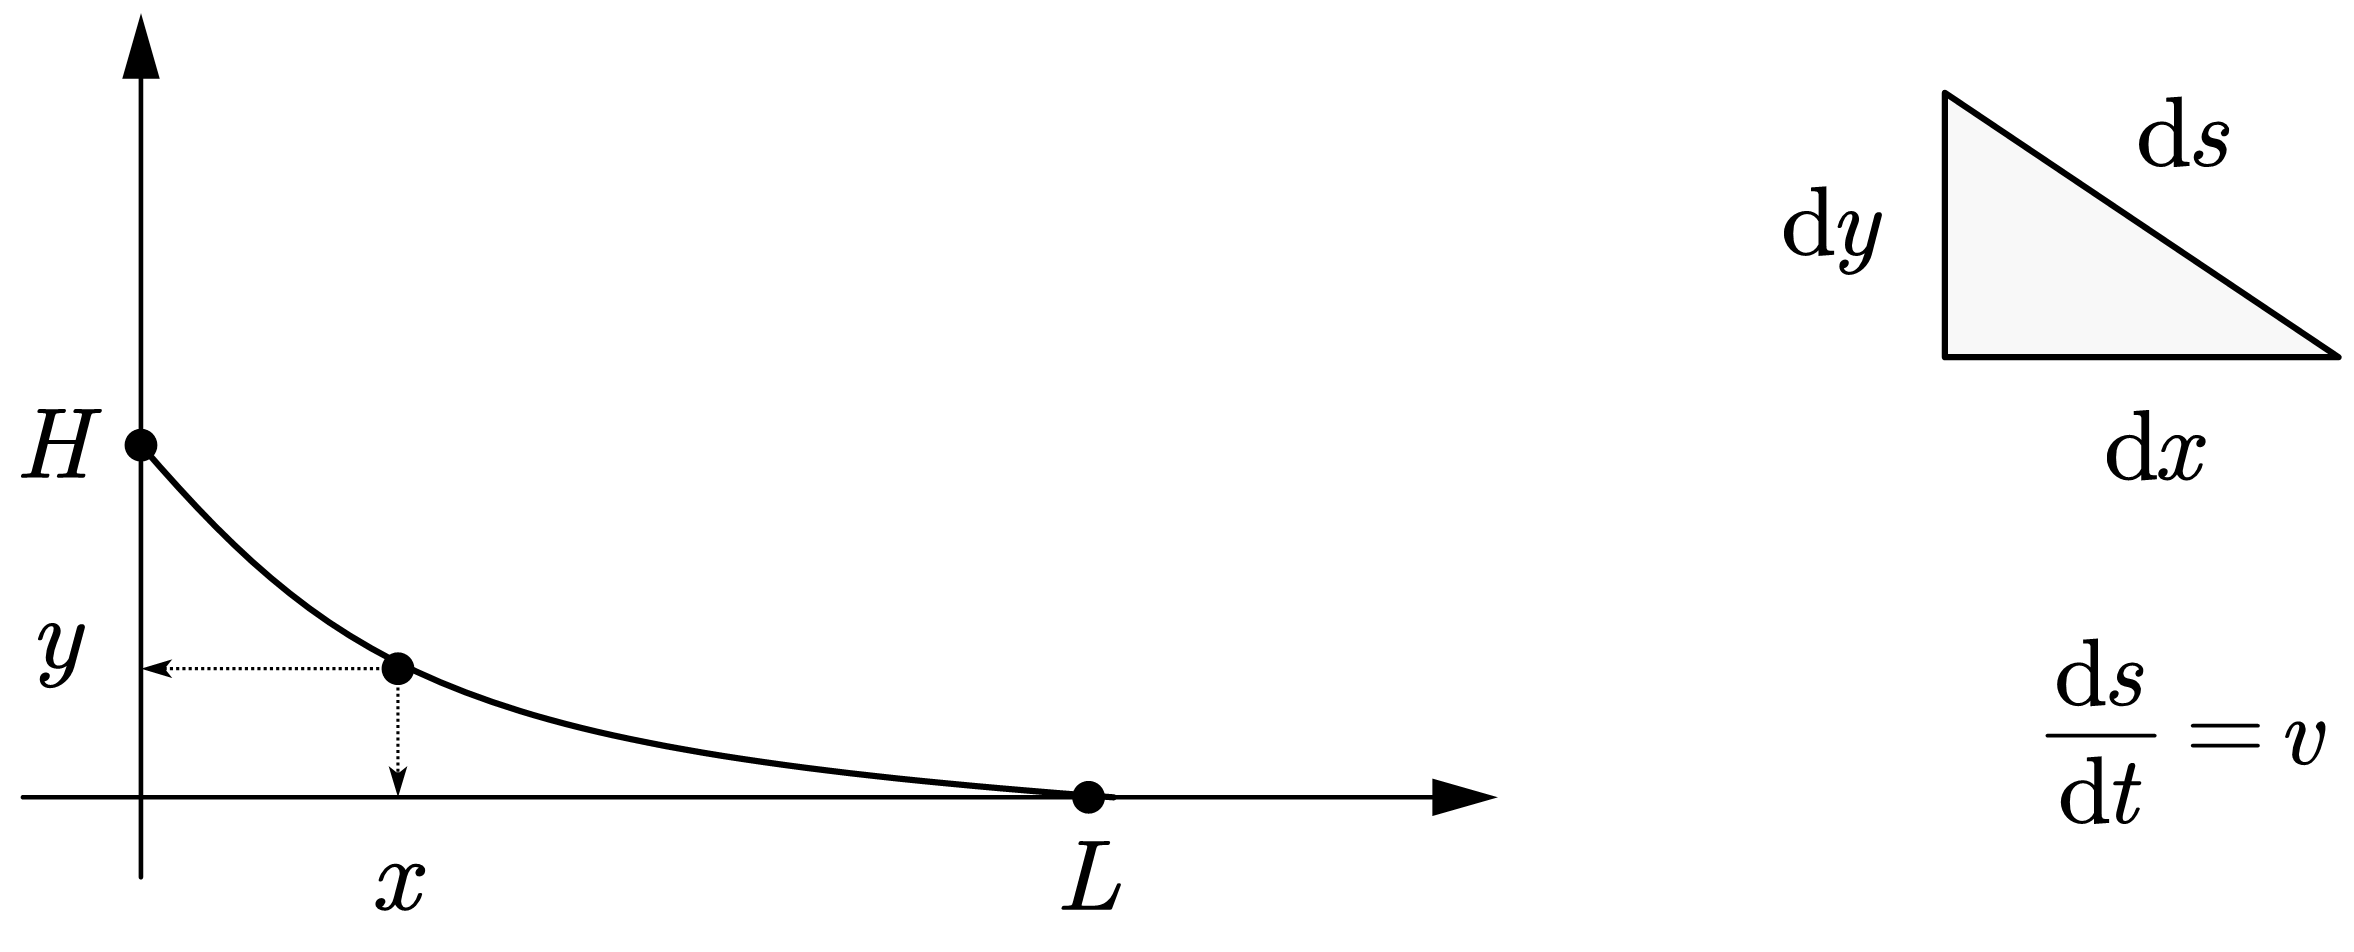
\includegraphics[width=8cm]{figure/fastest-path.png}
\end{center}
求最速降线方程,这条线也叫Brachistochrone curve。需要强调,图中只是一种示意,不代表路径必然在$x$轴上方,有可能某一部分是在下方的。
\end{example}
\begin{solution}
我们的求解目标是:
$$\min \int_0^T\dif t,\quad y(x=0)=H,y(x=L)=0$$
但积分是要对$x$进行的,因此需要得到$\dif t,\dif x$的关系式。如示意图所示,根据能量守恒有:
\begin{empheq}{equation}\label{fastest-desc-path-dx-dt}
\odv{s}{t}=v=\sqrt{2g(H-y)}=\frac{\dif x\sqrt{1+(y')^2}}{t}\ \implies \ \dif t=\sqrt{\frac{1+(y')^2}{2g(H-y)}}\dif x
\end{empheq}

于是现在的优化目标是:
\begin{empheq}{equation}\label{fastest-desc-path-target-transform}
\min_y\quad \int_0^L\sqrt{\frac{1+(y')^2}{2g(H-y)}}\dif x
\end{empheq}

可以忽略常数$g$。根据不显含$x$的特殊一阶条件\cref{1d-varition-min-1st-order-cond-special-1},可得:
$$\sqrt{\frac{1+(y')^2}{(H-y)}}-\frac{1}{\sqrt{(1+(y')^2)(H-y)}}(y')^2=C$$
左边为
$$\inv{\sqrt{H-y}}\inv{\sqrt{1+(y')^2}}>0$$
因此$C>0$。上式还可转化为:
\begin{empheq}{equation}\label{fastest-path-cond-deriv}
1+(y')^2=\inv{C^2}\inv{(H-y)}
\end{empheq}
由于$1+(y')^2\geq1$,因此$C^2(H-y)\leq 1$。

解上式时,可以直接解出$y'$,再解微分方程。另一种技巧是换元
\begin{empheq}{equation}\label{fastest-desc-path-target(theta)}
H-y=\inv{C^2}\sin^2\theta\implies 1+(y')^2=\inv{\sin^2\theta},\frac{1+(y')^2}{H-y}=\frac{C^2}{\sin^4\theta}
\end{empheq}
不妨取$\theta\geq 0$。同时根据上式有
\begin{empheq}{equation}\label{fastest-desc-path-target(theta)}
y'=-\inv{C^2}\sin(2\theta)\theta'
\end{empheq}
代入式\cref{fastest-desc-path-target(theta)},即有:
\begin{empheq}{equation}\label{fastest-desc-path-dtheta-dx}
\odv{\theta}{x}=\theta'=\pm\frac{C^2}{2\sin^2\theta}
\end{empheq}
可以解出
\begin{empheq}{equation}\label{fastest-desc-path-x-theta}
C^2x+C_1=\pm\left(\theta-\inv{2}\sin(2\theta)\right)
\end{empheq}

现在考虑定解条件:$x=0, y=H\implies\theta=0\implies C_1=0$。当$x=L$时,$y=0,H=\inv{C^2}\sin^2(\theta),C^2L=\pm\left(\theta-\inv{2}\sin(2\theta)\right)$。

分开考虑,$L>0$时,$4C^2L>0$,取$4C^2L=\theta-\inv{2}\sin(2\theta)$,结合$HC^2=\sin^2\theta$,有:
\begin{empheq}{equation}\label{fastest-desc-path-theta-max}
\frac{L}{H}=\frac{\theta-\inv{2}\sin(2\theta)}{\sin^2\theta}
\end{empheq}
据此可以解出$\theta_{\max}$,同时得到
\begin{empheq}{equation}\label{fastest-desc-path-C}
C=\sqrt{\frac{\sin^2\theta_{\max}}{H}}
\end{empheq}
则可以得参数方程形式的解:
\begin{empheq}[left=\empheqlbrace]{align}
x(\theta)&=\frac{1}{C^2}(\theta-\inv{2}\sin(2\theta))\\
y(\theta)&=H-\frac{\sin^2\theta}{C^2}\\
\theta&\in[0,\theta_{\max}]
\end{empheq}
当$L<0$时,$x$取反即可。或者让$x$乘上一个因子$\sign(L)$。这里需要注意,$x$是$\theta$的单调函数,但$y$不是。根据这个解,可以直接得到$\dot{x}(0)=0,\dot{y}(0)=0$。

能否根据$\sin\theta=\sqrt{C^2(H-y)},\theta=\arcsin \sqrt{C^2(H-y)}$代入$2C^2L$的等式解出$C$呢?这不太容易,因为一般来说$\arcsin\in\left[-\frac{\pi}{2},\frac{\pi}{2}\right]$,但本例中$\theta$是可以大于$\hpi$的,于是不一定能解出$C$。 

这是说周期函数的反函数不是单值函数,最好不要用。

\end{solution}

\paragraph*{坐标-时间}现在考虑运动时间。根据解可直接得到:
\begin{empheq}[left=\empheqlbrace]{align}\label{fastest-desc-path-xy-dot}
\dot{x}&=\frac{2\sin^2\theta}{C^2}\dot{\theta}\\
\dot{y}&=-\frac{\sin(2\theta)}{C^2}\dot{\theta}
\end{empheq}

需要求出$\dot{\theta}$。不妨假定$L>0$。则由\cref{fastest-desc-path-dtheta-dx}得到:
\begin{empheq}{equation}
\dif x=\frac{2\sin^2\theta}{C^2}\dif \theta
\end{empheq}

再根据式\cref{fastest-desc-path-target(theta)}给出的被积函数与$\theta$的关系式,可知:
\begin{empheq}{align}
t(x)&=\int_0^x \sqrt{\frac{1+(y')^2}{2g(H-y)}}\dif x\\
&=\int_0^{x^{-1}(x)}\inv{\sqrt{2g}} \frac{C}{\sin^2\theta}\frac{2\sin^2\theta}{C^2}\dif \theta\\
&=\frac{2}{\sqrt{2g}C}x^{-1}(x)
\end{empheq}
这里给出了时间与$x$坐标的关系。反之,$\theta$与$t$的关系就是:
\begin{empheq}{equation}
x(t)=x\left(\frac{\sqrt{2g}C}{2}t\right)\implies
\theta(t)=\frac{\sqrt{2g}C}{2}t
\end{empheq}
顺便也得到了$y(t)$。

最长运动时间
\begin{empheq}{equation}
t_{\max}=\frac{2}{\sqrt{2g}C}\theta_{\max}
\end{empheq}

\paragraph*{验证能量守恒}
现在验证此时$\sqrt{(\dot{x})^2+(\dot{y})^2}\stackrel{?}{=}\sqrt{2g(H-y)}$,即由能量守恒给出的速度是否与运动方程给出的相同。
\begin{empheq}{align}
\sqrt{(\dot{x})^2+(\dot{y})^2}&=\sqrt{\left(\frac{2\sin^2\theta}{C^2}\right)^2+\left(-\frac{\sin(2\theta)}{C^2}\right)^2}\frac{\sqrt{2g}C}{2}\\
&=\sqrt{2g}\frac{\sin\theta}{C}\\
\sqrt{2g(H-y)}&=\sqrt{2g}\sqrt{\frac{\sin^2\theta}{C^2}}\\
&=\sqrt{2g}\frac{\sin\theta}{C}
\end{empheq}
两式相等,能量守恒成立。

\paragraph*{特殊情况}现在来考虑一个问题,给定$H$,假如我们希望到达底部时,$\dot{y}=0$,也就是速度平行于$x$轴,则$L$应当怎么取?

根据式\cref{fastest-desc-path-xy-dot}有:
\begin{empheq}{equation}
\dot{y}=-\inv{C^2}\sin(2\theta)\dot{\theta}=0
\end{empheq}
由于$\dot{\theta}>0$,因此必有$\theta_{\max}=\hpi$。回代到\cref{fastest-desc-path-theta-max,fastest-desc-path-C},即有:
\begin{empheq}{align}
\frac{L}{H}&=\frac{\pi}{2}\\
C&=\inv{\sqrt{H}}
\end{empheq}

\paragraph*{数值解}
\begin{center}
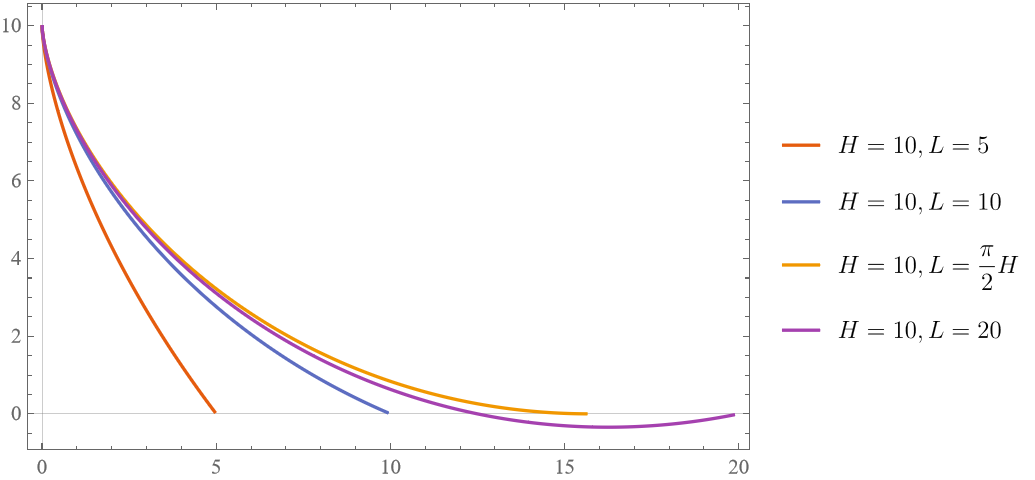
\includegraphics[width=10cm]{figure/fastest-descedning.png}
\end{center}

\subsubsection{最速升线}
\paragraph*{无约束}
\begin{example}
有最速降线,就有最速升线。如图所示:
\begin{center}
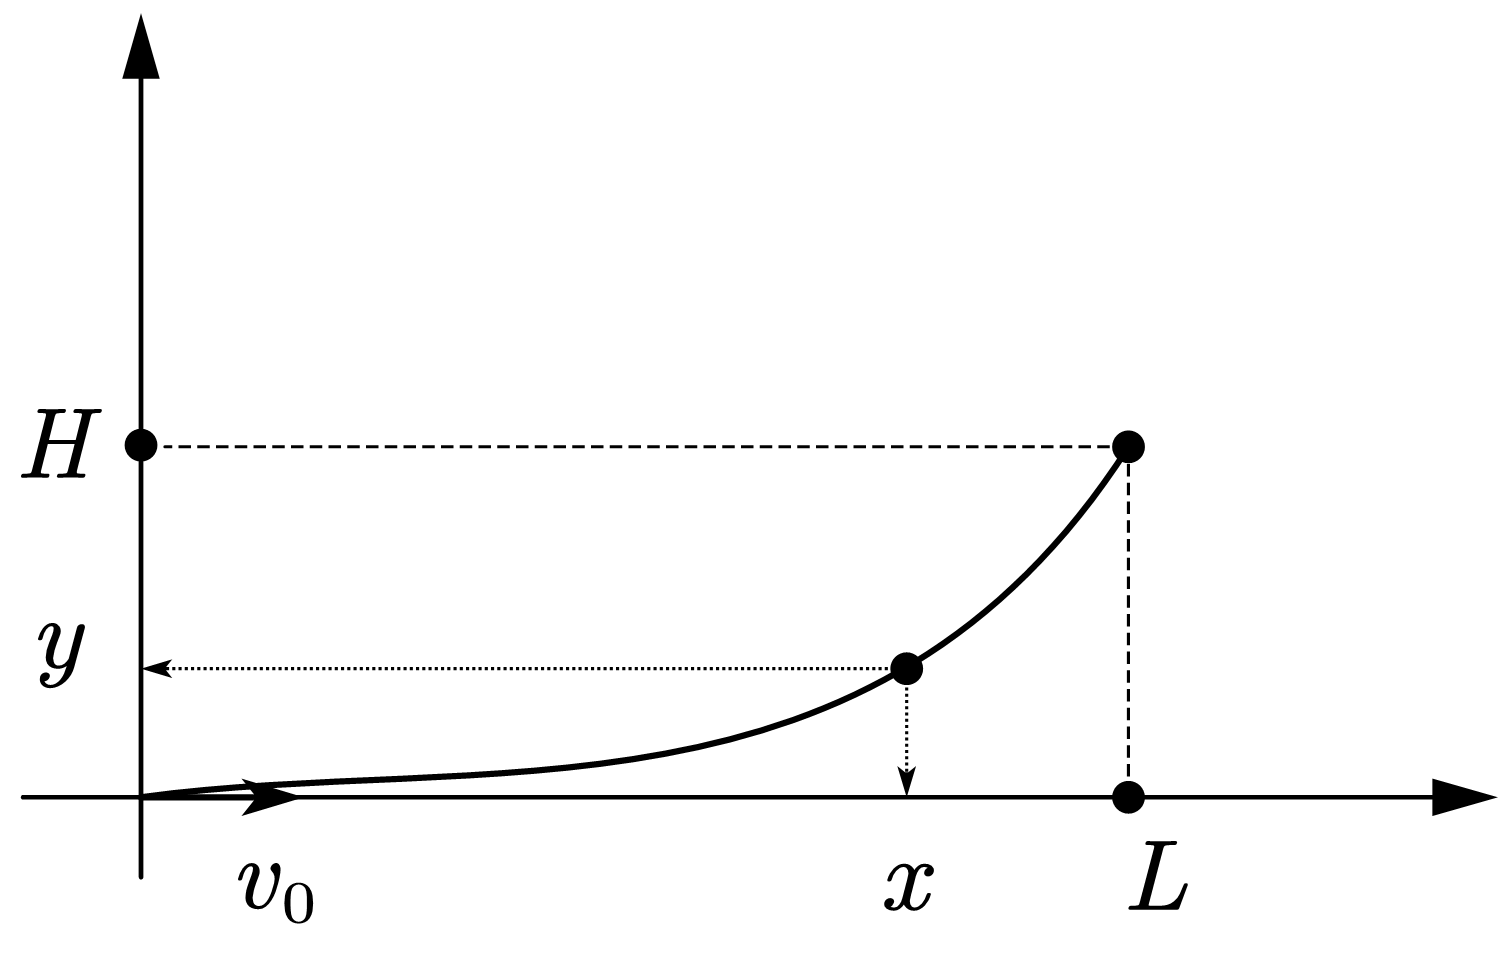
\includegraphics[width=6cm]{figure/fastest-ascending.png}
\end{center}
假定初始速度$v_0$,出发点为原点。显然,边界条件为$y(x=0)=0,y(x=L)=H$。
\end{example}
\begin{solution}
仍然沿用之前的做法,只是根据能量守恒,现在
$$v=\sqrt{2g\left(\frac{v_0^2}{2g}-y\right)}$$
$H$满足的限制为:
$$H\leq\frac{v_0^2}{2g}$$
对比最速降线中的速度\cref{fastest-desc-path-dx-dt},可知,现在的被积函数只是把$H$换成$\frac{v_0^2}{2g}$,此外边界条件有所改变,因此最后得到的是最速降线的一个镜像对称。

直到最速降线的\cref{fastest-desc-path-x-theta}的推导都是相同的,只是把被积表达式中的$H$换成$\frac{v_0^2}{2g}$。关键结论如下:
\begin{empheq}{align}
\frac{v_0^2}{2g}-y&=\frac{\sin^2\theta}{C^2}\implies 1+(y')^2=\inv{\sin^2\theta},\frac{1+(y')^2}{\frac{v_0^2}{2g}-y}=\frac{C^2}{\sin^4\theta}\label{fastest-asc-transform}\\
C^2x+C_1&=\pm\left(\theta-\inv{2}\sin(2\theta)\right)\label{fastest-asc-x-eq}
\end{empheq}

直接考虑定解条件。由两个边界条件代入换元表达式\cref{fastest-asc-transform}有:
\begin{empheq}{align}
\frac{v_0^2}{2g}&=\frac{\sin^2\theta_0}{C^2}\\
\frac{v_0^2}{2g}-H&=\frac{\sin^2\theta_1}{C^2}
\end{empheq}
易知$\sin^2\theta_1<\sin^2\theta_0$,由于$\theta>0$,因此$\theta_1<\theta_0$。再把两个边界条件代入\cref{fastest-asc-x-eq},有:
\begin{empheq}{align}
C_1&=\pm\left(\theta_0-\inv{2}\sin(2\theta_0)\right)\\
C^2L+C_1&=\pm\left(\theta_1-\inv{2}\sin(2\theta_1)\right)
\end{empheq}
未知数为$\theta_0,\theta_1,C,C_1$,恰有4个方程,可以求解。当$L>0$时,$C^2L+C_1>C_1$,再加上$\theta_1<\theta_0$,因此应该取$-$。使用数值计算时,约束条件为$C>0,2\pi>\theta_0>\theta_1>0$。

在已经解出系数的情况下,曲线为:
\begin{empheq}[left=\empheqlbrace]{align}
x(\theta)&=-\frac{1}{C^2}\left(\theta-\inv{2}\sin(2\theta)+C_1\right)\\
y(\theta)&=\frac{v_0^2}{2g}-\frac{\sin^2\theta}{C^2}\\
\theta&\in[\theta_0,\theta_1]
\end{empheq}
速度与时间的方程为:
\begin{empheq}[left=\empheqlbrace]{align}\label{fastest-asc-path-xy-dot}
\dot{x}&=-\frac{2\sin^2\theta}{C^2}\dot{\theta}\\
\dot{y}&=-\frac{\sin(2\theta)}{C^2}\dot{\theta}
\end{empheq}
现在求$\dot{\theta}$。
\begin{empheq}{align}
t(x)&=\int_0^x \sqrt{\frac{1+(y')^2}{2g(H-y)}}\dif x\\
&=\int_{x^{-1}(x)}^{\theta_0}\inv{\sqrt{2g}} \frac{C}{\sin^2\theta}\frac{2\sin^2\theta}{C^2}\dif \theta\\
&=\frac{2}{\sqrt{2g}C}(\theta_0-x^{-1}(x))\\
\implies x(t)&=x\left(\theta_0-\frac{\sqrt{2g}C}{2}t\right)\\
t_{\max}&=\frac{2}{\sqrt{2g}C}(\theta_0-\theta_1))
\end{empheq}
注意以上$x^{-1}(x)<\theta_0$,要保持积分为正,需要交换上下限。

能量守恒的验证与最速降线相同。

以上的做法,有一个问题是,速度是以绝对值进入模型的,因此没有方向,所以不能实现速度水平的约束。


\end{solution}

\paragraph*{特殊情况}如果要求$\dot{y}(\theta_0)=0$,则$\theta_0=\hpi,C=\sqrt{\frac{2g}{v_0^2}},C_1=\hpi,\theta_1=\arcsin\sqrt{1-\frac{2gH}{v_0^2}}$,最后
$$L=-\inv{C^2}\left(\theta_1-\inv{2}\sin(2\theta_1)+C_1\right)$$
\paragraph*{数值解}
\begin{center}
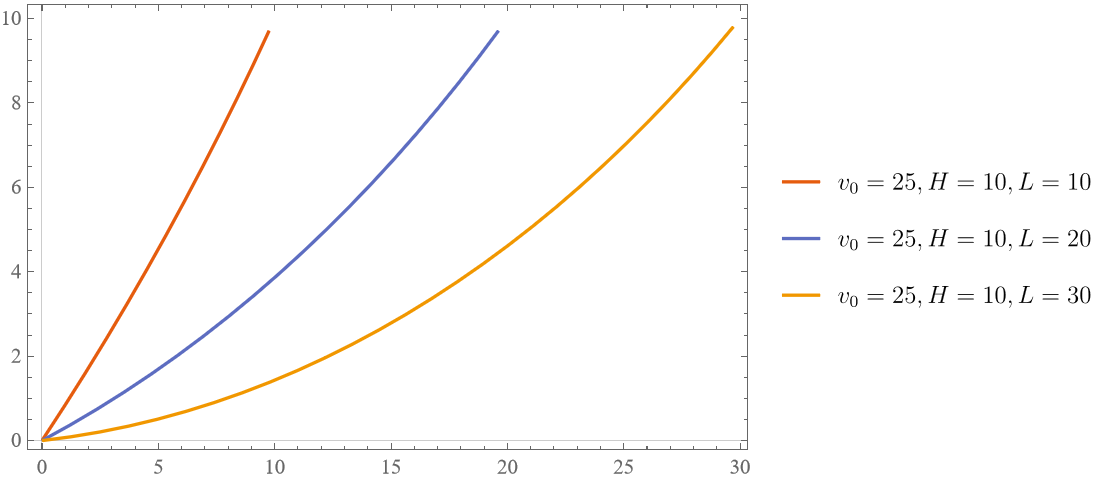
\includegraphics[width=10cm]{figure/fastest-ascedning.png}
\end{center}

\paragraph*{水平初速度约束}
\begin{example}
无约束最速升线的基础上,限定初速度与$x$轴平等,再次求解。
\end{example}
\begin{solution}

\end{solution}
\subsubsection{连续问题的一阶欧拉拉格朗日方程}
给定单变量函数优化问题

\begin{empheq}[left=\empheqlbrace]{align*}
\min_{\bm{q}}&\int_{t_0}^{t_1}L(\bm{q}(t),\bm{q}'(t),t)\\
\bm{q}(t_0)&=\bm{a}\\
\bm{q}(t_1)&=\bm{b}\\
\bm{q}&\colon \mathbb{R}\rightarrow \mathbb{R}^K
\end{empheq}

它等价于下面的欧拉-拉格朗日方程:
$$\frac{\dif }{\dif t}L_{\bm{q}_j'}(\bm{q},\bm{q}',t)-L_{\bm{q}_j'}(\bm{q},\bm{q}',t)=0,j=1\cdots,K$$

跟凸优化类似.注意,仅求解方程实际上并不能一定说解就是最小化原问题的解.更确切地说是求得驻点或者是潜在的稳态解.另外对$L$求导时,我们把$\bm{q}'$当作变量,并非链式法则.

多变量时,结果类似.问题

\begin{empheq}[left=\empheqlbrace]{align*}
	\min_{\bm{q}}&\int_{t_0}^{t_1}L(\bm{q},\partial \bm{q},\bm{x})\dif \bx\\
	\bm{q}&=\bm{\phi},\text{在}\partial D\text{上}\\
	\bm{q}&\colon \mathbb{R}^N\rightarrow \mathbb{R}^K
\end{empheq}

欧拉-拉格朗日方程为
$$\sum_{k=1}^n \partial_j L_{\partial_j \bm{q}_k}-L_{\bm{q}_k}=0,k=1,\cdots,K$$

注意这里是求和,单变量问题中只有一个变量,就没有求和.

\chapter{微分方程与动力系统}\label{ode-dynamic-system}
\section{常微分方程}
\subsection{常微分方程的求解}
\subsubsection{一览表}
\begin{longtable}{cl}
\toprule
\bf{方程形式}& \hfill\bf{解}\\
\midrule
$y'(x)+p(x)y=q(x)$& $y=e^{-\int p(x)\dif x}\left(\int q(x)e^{-\int p(x)\dif x}+C\right)$\\
\midrule
\multirow{5}{*}{$ay''+by'+cy=0$}&首先求解特征方程:$ar^2+br+c=0$,得到两个解$r_1,r_2$:\\
&\circled{1} $r_1,r_2$为两个不等实根,则$y=C_1e^{r_1x}+C_2e^{r_2x}$\\
&\circled{2} $r_1=r_2=r$,为重根,则$y=C_1e^{rx}+C_2xe^{rx}$\\
&\circled{3} $r_1,r_2$为两个纯虚根$\pm i\omega$,则$y=C_1\cos(\omega x)+C_2\sin(\omega x)$\\
&\circled{4} $r_1,r_2$为两个复根$r\pm i\omega $,则$y=e^{rx}(C_1\cos(\omega x)+C_2\sin(\omega x))$\\
\bottomrule
\end{longtable}

\subsection{Lyapunov稳定性理论}\label{ode-lyapunov}
Lyapunov理论主要用来考查常微分方程
\begin{equation}\label{lyapunov-ode}
\dot{\bx}=\bm{f}(t,\bx),\bx(t_ 0)=\bx_0
\end{equation}
的稳定性。

首先要定义什么是稳定性。

\subsubsection{Lyapunov稳定性}
\begin{theorem}[Lyapunov稳定性]
\begin{description}
\item[平衡点] $\bx^*$称为平衡点,如果$\forall t\geq 0, f(\bx^*,t)=0$。
\item[稳定] 一个平衡点$\bx_e$称为稳定的,如果$\forall t_0\geq 0,\epsilon>0$,存在标量$\delta(t_0,\epsilon)$满足
$$\|\bx_0-\bx_e\|<\delta \implies \forall t>t_0,\|\bx_t-\bx_e\|<\epsilon$$
含义是说如果初始点接近平衡点,则轨迹始终停留在距离平衡点的一个小区域内。
\item[一致稳定] 在稳定的定义中,如果$\delta$可以与$t_0$无关,则称为一致稳定。
\item[渐近稳定] $\bx_e$稳定且为吸引子。\textbf{吸引子}定义为:$\forall t_0\geq 0$,存在$\delta(t_0)$满足
$$\|\bx_0-\bx_e\|<\delta \implies \lim_{t\rightarrow \infty}\|\bx_t-\bx_e\|=0$$
吸引子的含义是说如果初始点距离平衡点够近,则最终轨迹收敛于平衡点。
\item[一致渐近稳定] $\bx_e$一致稳定且轨迹一致收敛于$\bx_e$。后者定义为存在$\delta>0$和一个函数$\mathbb{R}_+\times \mathbb{R}^n\rightarrow \mathbb{R}_+$,$\gamma$满足$\forall \bx_0\in B_{\delta},\lim_{\tau\rightarrow \infty}\gamma(\tau,\bx_0)=0$。然后有
$$\|\bx_0-\bx_e\|<\delta \implies \|\bx_t-\bx_e\|\leq \gamma(t-t_0,\bx_0)$$
这里与一致稳定加上渐近稳定非常像,只是在渐近的定义上有所不同,渐近稳定中考虑的是极限,而一致渐近稳定考虑的是距离的上界,$\gamma$刻画了收敛速率。
\item[全局渐近稳定] $\bx_e$稳定且$\forall \bx_0\in\Rns,\lim_{t\rightarrow\infty} \bx_t=\bx_e$.含义为对于\emph{任意}初始值,轨迹最终趋于$\bx_e$。
\item[指数稳定] $\bx_e$稳定,且存在$m,\alpha>0$,满足
$$\forall \bx_0\in B_h,t\geq t_0\geq 0,\|\bx_t-\bx_e\|\leq me^{-\alpha(t-t_0)}\|\bx_0\|$$
$B_h$是$\bx_e$的邻域,$\alpha$称为收敛速率。含义是轨迹与均衡点的距离按指数衰减。

大致可以看出,指数稳定是渐近稳定的特例。
\end{description}
\end{theorem}
以上的定义中上,核心点主要有三个:稳定、吸引子、指数稳定。稳定与吸引子容易混淆。前者指的是轨迹始终停留在一个小区域内,而后者说的是极限情况。吸引不一定稳定,因为在中途,轨迹可能脱离这个小区域,也就是说无论初始距离取得多么近,在收敛之前,它会脱离小区域。

稳定也不一定吸引,可能在平衡点附近一直波动,但就是不收敛。
\subsubsection{能量函数}
\begin{definition}[能量函数与正定函数]
一个连续、严格\emph{单调递增}函数,且满足$\alpha(0)=0$的函数$\alpha:\mathbb{R}^+\rightarrow \mathbb{R}^+$称为{\heiti K族函数}(隐含$\alpha(\cdot)>0$。如果它还满足当$p\rightarrow \infty$时,有$\alpha(p)\rightarrow \infty$,则称之为{\heiti KR函数}。

一个连续函数$v(\bx,t): \mathbb{R}^n\times \mathbb{R}_+\rightarrow \mathbb{R}_+$称为{\heiti 局部正定函数}(l.p.d.f),如果它满足,对于一些$h>0$和一些$K$函数$\alpha$,有:
$$v(0,t)=0,\text{且} \forall \bx\in B_h,t>0, v(\bx,t)\geq \alpha(|\bx|)$$

一个l.p.d.f局部地像一个能量函数。而一个{\heiti 正定函数}全局地像{\heiti 能量函数}。

具体地说,一个连续函数$v(\bx,t): \mathbb{R}^n\times \mathbb{R}_+\rightarrow \mathbb{R}_+$称为 正定函数(p.d.f),如果它满足,对于一些KR函数$\alpha$,有
$$v(0,t)=0,\text{且}\forall \bx\in\mathbb{R}^n,t\geq 0, \text{有}v(\bx,t)\geq \alpha(|\bx|)$$

同时还有{\heiti 减函数}。一个连续函数$v(\bx,t): \mathbb{R}^n\times \mathbb{R}_+\rightarrow \mathbb{R}_+$称为减函数(decrescent函数)。如果存在一些K函数$\beta$,满足
$$\forall \bx\in B_h,t\geq 0,v(\bx,t)\leq\beta(|\bx|)$$
\end{definition}
局部正定函数相当于在局部,函数的下界为一个单调递增函数(准确地说是K函数),或大于一个$K$函数。而正定函数是全局性的,含义为函数全局地大于一个KR函数。减函数是说函数小于一个K函数。

局部正定函数与正定函数的区别在于下界的性质和$\bx$的范围。

\begin{example}
以下给出一些能量函数的例子:
\begin{enumerate}
\item $|\bx|^2$:减p.d.f.
\item $\bx^TP\bx$,$P$正定矩阵:减p.d.f.。$\lambda_{\min} |\bx|^2\leq  \bx^TP\bx\leq \lambda_{\max}|\bx|^2$。
\item $(t+1)|\bx|^2$:p.d.f.$(t+1)|\bx|^2\geq |\bx|^2$。
\item $e^{-t}|\bx|^2$:减函数。上界可以取$e^{-t_0}|\bx|^2$.
\item $\sin^2(|\bx|^2)$:减l.p.d.f.
\item $e^t\bx^TP\bx$,$P$不正定:以上全不是。
\item $v(\bx,t)$与$t$无关,则它为减函数。
\end{enumerate}
\end{example}


\subsubsection{基本Lyapunov定理}
\begin{theorem}[基本Lyapunov定理]
对于任意能量函数,以下给出了判断ODE\eqref{lyapunov-ode}稳定性的条件:
\begin{longtable}{|c|c|c|}
\hline
$v$ & $-\dot{v}$ & \textbf{结论}\\
\hline
l.p.d.f. & 局部$\geq 0$ &稳定\\
减l.p.d.f. & 局部$\geq 0$ & 一致稳定\\
减l.p.d.f. & l.p.d.f. & 一致渐近稳定\\
减p.d.f. & p.d.f. &全局一致渐近稳定\\
\hline 
\end{longtable}

其中
$$\dot{v}=\sum_{i=1}^n\pdv{v}{x_i}f_i+\pdv{v}{t}$$

需要强调,以上给出的是一个充分而非必要条件,如果一个Lyapunov函数下,以上条件不满足,只能说在这个函数下不能给出稳定性;但在其它函数下仍然可能稳定。
\end{theorem}

\subsubsection{不稳定性}
\paragraph*{自治系统}以下几个定理涉及$f$与时间无关的ODE:
\begin{equation}
\dot{x}=f(\bx),\bx(t_0)=\bx_0
\end{equation}

\begin{theorem}[Lyapunov不稳定性定理]
记$\bx_e$为一平衡点。如果存在一个函数$V:\mathbb{R}^n\rightarrow \mathbb{R}$,满足:
\begin{enumerate}
\item $\forall \bx\in\{\bx:V(\bx)\leq 0\}, \dot{V(\bx)}\leq 0$.注意这里$\bx$是$t$的函数。
\item $V(x_0)< V(\bx_e)$
\end{enumerate}
则轨迹$\bx(t)$不会收敛于$\bx_e$。
\end{theorem}

以上定理其实比较简单,因为初始的能量小于$V(\bx_e)$,而$\dot{V}$又是小于等于0的,所以随着时间的发展,能量会起来越小,且小于$V(\bx_e)$,自然不会收敛于$\bx_e$。

\begin{theorem}[Lyapunov发散定理]
记$\bx_e$为一平衡点。如果存在一个函数$V:\mathbb{R}^n\rightarrow \mathbb{R}$,满足:
\begin{enumerate}
\item $\forall \bx\in\{\bx:V(\bx)< 0\}, \dot{V(\bx)}< 0$
\item $V(x_0)< 0$
\end{enumerate}
则轨迹$\bx(t)$无界。
\end{theorem}

这个定理也比较简单。首先必然有$V(\bx(t))<V(\bx_0)$,这与$\dot{V(\bx)}<0$和初始值 $V(x_0)< 0$有关。现在假设轨迹有界,即$\|\bx(t)\|\leq R$,那么集合$\{\bx:V(\bx)\leq V(\bx_0),\|\bx\|\leq R\}$为紧致集合,则有正数$\beta$满足$-\dot{V}\leq -\beta$,于是$V(\bx(t))\leq V(\bx_0)-\beta t$,那么$V(\bx(t))\rightarrow \infty$,因此无界。


\subsubsection{分析案例}
\paragraph*{塌缩函数}此处是指形如$\bm{f}(\bx,t)=\bm{g}(s(\bx),t)$,即向量$\bx$最终可以归结为一个标量进入模型。

\begin{example}
什么
\end{example}

\paragraph*{非塌缩函数}

\begin{example}
\begin{empheq}[left=\empheqlbrace]{align*}
\dot{x_1}&=x_2\\
\dot{x_2}&=-x_2-(2+\sin t)x_1
\end{empheq}
显然$\bm{0}$为平衡点。取能量函数
$$v(\bx,t)=x_1^2+\frac{x_2^2}{2+\sin t}$$
由于
$$x_1^2+x_2^2=|\bx|^2\geq v(\bx,t)\geq x_1^2+x_2^2/3\geq 1/3|\bx|^2$$
因此它是减p.d.f.。

再考虑$-\dot{v}$:
$$-\dot{v}=\frac{x_2^2(4+2\sin t+\cos t)}{(2+\sin t)^2}\geq 0$$
因此是一致稳定的。但不是一致渐近稳定,因为$-\dot{v}$只与$\bx_2$有关,找不到一个函数K函数$\alpha(|\bx|)$,使得$-\dot{v}$的下界为它。
\end{example}

\begin{example}
{\heiti 极限环系统}

\begin{empheq}[left=\empheqlbrace]{align*}
\dot{x_1}&=-x_2+x_1(x_1^2+x_2^2-1)\\
\dot{x_2}&=x_1+x_2(x_1^2+x_2^2-1)
\end{empheq}
显然$\bm{0}$为平衡点。取能量函数
$$v(\bx,t)=x_1^2+x_2^2$$
它是减p.d.f.。

再考虑$-\dot{v}$:
$$-\dot{v}=-2(x_1^2+x_2^2)(x_1^2+x_2^2-1)=-2|\bx|^2(|\bx|^2-1)$$
在$|\bx|<1$的范围内,$-\dot{v}$相对于$|\bx|$单调递增;在较大的范围内,$-\dot{v}<0$,因此只是l.p.d.f.。所以$\bm{0}$是一致渐近稳定的,但不是全局一致渐近稳定。
\end{example}
\subsection{其它稳定性理论}
\subsubsection{线性方程与线性近似的稳定性}
\begin{theorem}[线性ODE方程的稳定性]
一个线性方程
$$\dot{\bx}=A\bx$$
则它的稳定性与$A$的特征值密切相关:
\begin{enumerate}
\item $\bx=0$渐近稳定$\iff \forall \lambda_i(A),\Re(\lambda_i)<0$,即特征值实部全为负。
\item $\bx=0$稳定$\iff \Re(\lambda_i)\leq 0$,且实部为负的特征根对应的Jordan块为一阶。
\item $\bx=0$不稳定$\iff \exists \lambda_i, \Re(\lambda_i)>0$
\end{enumerate}
\end{theorem}

线性方程的稳定性与线性近似的稳定性密切相关:

\begin{theorem}[线性近似的稳定性]
如果$\bm{f}$是非线性的,则在平衡点附近进行线性化:
$$\dot{\bx}=A(t)\bx+\bm{N}(t,\bx)$$

$\bm{N}$满足
\begin{enumerate}
\item $N(t_0, \bx_e)=0$
\item $\forall t\geq t_0,\lim_{|\bx|\rightarrow|\bx_e|}\frac{|N(t,\bx)|}{|\bx|}=0$
\end{enumerate}

如果$A(t)=A$为一常矩阵,则原来的非线性方程的稳定性与线性化后的方程的稳定性相关:
\begin{enumerate}
\item $\bx=0$渐近稳定$\iff \forall \lambda_i(A),\Re(\lambda_i)<0$,即特征值实部全为负。
\item $\bx=0$不稳定$\iff \exists \lambda_i, \Re(\lambda_i)>0$
\end{enumerate}

需要注意,线性近似法相比纯线性方程的稳定性的区别在于:线性挖只适用于\emph{渐近稳定}与\emph{不稳定}的情形,不能判别稳定。

如果$A(t)$不为常矩阵,则没有以上结论。
\end{theorem}




\subsection{不稳定性理论}
\subsubsection{爆破}

\subsubsection{刚性}

\subsubsection{极限环}

\section{偏微分方程}

\subsection{概论}
\subsubsection{PDE的分类理论}
偏微分方程就是指含有多个自变量的导数的方程。

\paragraph*{一阶PDE}只含有一阶导数的PDE,形如
$$\sum a_i(\bx)\pdv{u(\bx)}{x_i}=F(u)$$
的称为一阶线性PDE。如果$a_i$与$u$有关,形如:
$$\sum a_i(\bx,u(\bx))\pdv{u(\bx)}{x_i}=F(u)$$
的称为一阶拟线性PDE。不是线性、拟线性的叫一阶非线性PDE。

\paragraph*{二阶PDE}最高含有二阶导数的PDE为线性PDE。$n$个自变量(时间$t$也算其中的一个)的二阶线性PDE的一般形式为:
\begin{empheq}{equation}
\sum_{i=1}^n\sum_{i=1}^na_{ij}\pdv[order=2]{u}{x,y}+\sum_{i=1}^nb_i\pdv{u}{x_i}+cu(\bx)=f
\end{empheq}
系数$a_{ij}$构成系数矩阵$A=[a_{ij}]$。依据系数矩阵在某点$\bx$处的特征值分布:
\begin{description}
\item[椭圆型] $A$的特征值同号。
\item[双曲型] $A$的特征值有$n-1$个同号,与剩下的一个异号。
\item[抛物型] 特征值有一个为0,其它同号。
\end{description}
称PDE在该点处为对应的型。如果PDE在整个区域内都为此型,即称为对应的PDE型;如果在某些部分为一型,另一些部分为其它型,称为混合型PDE。
\paragraph*{例子}以下给出一些PDE的例子与其对应的分类:
\begin{longtable}{ccc}
\toprule
名称 & 形式 & 说明\\
\midrule
拉普拉斯方程& $\Delta u=f$ & 二阶椭圆。\\
波动方程& $\pdv[order=2]{u}{t}-c^2\pdv[order=2]{u}{x}=0$ &二阶双曲。系数矩阵的特征值为$1,-c^2$。\\
热传导& $\pdv{u}{t}=k\pdv[order=2]{u}{x}$& 二阶抛物。\\
\bottomrule
\end{longtable}

\subsection{计算方法}


\subsection{分析方法}


\section{离散时间动力系统}
\subsection{表示论}
\subsubsection{常系数线性系统与矩阵乘法}
给定一个线性系统
$$y_{n+2}=2y_{n+1}+y_{n}$$
可以表示为矩阵乘法
\[
\begin{bmatrix}
y_{n+3}\\
y_{n+2}
\end{bmatrix}=\begin{bmatrix}
5 & 2\\
2 & 1
\end{bmatrix}\begin{bmatrix}
y_{n+1}\\
y_{n}
\end{bmatrix}\]

比如给定初始值$[y_0,y_1]=[1,1]$,那么直接迭代计算$y_4=17,y_5=41$,也可以用两次矩阵计算
\[\begin{bmatrix}
	y_{5}\\
	y_{4}
\end{bmatrix}=\begin{bmatrix}
	5 & 2\\
	2 & 1
\end{bmatrix}^2\begin{bmatrix}
	y_{1}\\
	y_{0}
\end{bmatrix}=\begin{bmatrix}
41\\17
\end{bmatrix}\]
利用矩阵乘法,一次可以计算2个值。显然原本的迭代增长速度是指数的,所以矩阵连乘可以表达指数增长。而且可以利用特征值分解来计算矩阵乘法。

那么一个显然的问题是,矩阵连乘能不能表示多项式增长?当然是可以的。

考虑矩阵
\[M=\begin{bmatrix}
	1 & 2\\
	0 & 1
\end{bmatrix}\]
可以算出
\[M^n=\begin{bmatrix}
	1 & 2n\\
	0 & 1
\end{bmatrix}\]
这是多项式增长的。而且注意到,其实$M$的特征值是2个1。

其实对于矩阵
\[
M=\begin{bmatrix}
1& a_{12} & a_{13}\\
0& 1 & a_{23}\\
0&0&1
\end{bmatrix},M^n=\begin{bmatrix}
1& na_{12} & \frac{n(n+1)}{2}a_{13}a_{23}+na_{13}\\
0& 1 & na_{23}\\
0&0&1
\end{bmatrix}
\]

可以看出是多项式增长的。一个简单的想法就是,对于三角阵,如果对角线上都是1,那就是多项式增长,这也部分说明了为什么对角线元素比较重要。

\subsubsection{使用矩阵或纯加法计算多项式}
一个多项式可以写成 $a_nx_1^n=a_n(x_0+\dif x)^n=a_n\sum_{k=0}^{n }\alpha_k x^k\dif^{n-k}x$的形式,其中$\alpha_k$是多项式系数。比如,

$$
\begin{bmatrix}
	a_4x_1^4\\
	a_4x_1^3\dif x\\
	a_4x_1^2\Dif2 x\\
	a_4x_1\Dif3 x\\
	\Dif4 x
\end{bmatrix}=\begin{bmatrix}
	\binom{4}{4} & \binom{4}{3} & \binom{4}{2} & \binom{4}{1} &\binom{4}{0}\\
	0& \binom{3}{3} & \binom{3}{2} &\binom{3}{1} &\binom{3}{0} \\
	0& 0& \binom{2}{2} & \binom{2}{1} & \binom{2}{0}\\
	0& 0&0& \binom{1}{1}&\binom{1}{0}\\
	0& 0& 0& 0& 1
\end{bmatrix}\begin{bmatrix}
	a_4x_0^4\\
	a_4x_0^3\dif x\\
	a_4x_0^2\Dif2 x\\
	a_4x_0\Dif3 x\\
	\Dif4 x
\end{bmatrix}=\begin{bmatrix}
	1 & 4 & 6 & 4 &1\\
	0& 1 & 3 &3 &1 \\
	0& 0& 1 & 2 & 1\\
	0& 0&0& 1&1\\
	0& 0& 0& 0& 1
\end{bmatrix}\begin{bmatrix}
	a_4x_0^4\\
	a_4x_0^3\dif x\\
	a_4x_0^2\Dif2 x\\
	a_4x_0\Dif3 x\\
	\Dif4 x
\end{bmatrix}
$$

通过矩阵连乘,我们可以计算 $x_i^n,i\geq 1$。不过这里还有标量乘法。假如只用加法,\circled{1} 希望矩阵的元素属于 $\{-1,0,1\}$,或者  \circled{2} 直接用加法代替乘法,需要 $2^4+2^3+2^2+2^1+2^0-\frac{(1+5)5}{2}$ 次加法来代替矩阵乘法。后者显然是不合适的。

现在来考虑一个更抽象的问题,计算:
$$\bm{y}_{n+1}=L\bm{y}_n \text{ ,且 } L \text{是上三角阵且} L_{ii}=1$$

考虑方法\circled{1}, 也就是通过基变换的方式。希望找到矩阵 $M,A$使得
$$A\by_{n+1}=MA\by_{n} \text{ 且 }M_{ij}\in\{-1,0,1\}$$
这样一来 $A\by_{n+1}=AL\by_n=MA\by_n$。一个简单的条件是$AL=MA$。注意上面这个变换的含义,$A$是变换矩阵,我们同时对$\by_{n+1},\by_n$进行变换,使得$A\by_{n+1}$恰好可以通过$A\by_n$进行行的加减法得到。

显然这个问题是不定的,因为参数过多。我们可以随便选择$M$ 然后求解$AL=MA$ 得到$A$ ,具体来说是求解$Px=0$ ,其中$x$ 是将 $A$中元素堆叠形成的向量。

在我们的问题中,需要计算 $a_4x^4$ ,它是$\by_n$的第一行。那么$A$的第一行应该是$[1,\bm{0}]$ ,也就是说我们寻找 的变换不改变 $\by_n$的第一行。并且 $M$ 必须是上三角阵,因为每一行为线性组合的系数,而高次项的线性组合不可能得到低次项。于是$\forall i<j, M_{ij}=0$。即使加上这些约束,问题还是不定的。 

现在我们考虑用尽可能少的加法,那么至少需要的加法次数是1。于是 $M$的形式应该像:
\[M=\begin{bmatrix}
	1 & 1 &  &  &  \\
	& 1& 1& &\\
	& & 1& 1& \\
	& & & 1& 1\\
	& & & & 1
\end{bmatrix}\]

由于$A$的第一行固定为$[1,\bm{0}]$,我们可以按顺序求解出 $A$的每一行。比如对于第二行可以构造方程:
$$\begin{aligned}
	\underbrace{\begin{bmatrix}
			1 & 0 & 0 & 0& 0\\
			0 & x_2 & x_3 & x_4 &x_5\\
	\end{bmatrix}}_{A}\underbrace{\begin{bmatrix}
			1 & 4 & 6 & 4 &1\\
			0& 1 & 3 &3 &1 \\
			0& 0& 1 & 2 & 1\\
			0& 0&0& 1&1\\
			0& 0& 0& 0& 1
	\end{bmatrix}}_{L}&=\underbrace{\begin{bmatrix}
			1 & 4 & 6 & 4 &1\\
			0& x_2& 3x_2+x_3&3x_2+2x_3+x_4&x_2+x_3+x_4+x_5
	\end{bmatrix}}_{P}\\
	=\underbrace{\begin{bmatrix}
			1 & 1 &  &  &  \\
			& 1& 1& &\\
			& & 1& 1& \\
			& & & 1& 1\\
			& & & & 1
	\end{bmatrix}}_{M}\underbrace{\begin{bmatrix}
			1 & 0 & 0 & 0& 0\\
			0& x_2 & x_3 & x_4 &x_5\\
	\end{bmatrix}}_{A}&=\underbrace{\begin{bmatrix}
			1 & x_2 & x_3 & x_4 &x_5\\
			& & \cdots & & 
	\end{bmatrix}}_{Q}
\end{aligned}
$$

对比$P$与$Q$,有$[1, x_2,x_3,x_4,x_5]=[1,4, 6,4,1]$。它恰好是$L$的第一行。那么$P$的第二行已经固定了。现在可以用$Q$的第2行求解$A$的第3行$\cdots$最终解出$A$的全部行。 用数学的语言来表示这个迭代过程:
\[\begin{aligned}
	P_{i,}&=A_{i,}L\\
	Q_{i,}&=A_{i,}+A_{i+1,}\\
	P_{i,}&=Q_{i,}
\\
	s.t.&\ A_{0,},L\text{ 已知}
\end{aligned}\]
其中 $A_{i,}$ 表示$A$的第$i$行。最终,
$$A_{i+1,}=P_{i,}-A_{i,}=A_{i,}L-A_{i,}=A_{i,}(L-I)$$ 

这样就求出了 $A$的每一行。最后就可以用 $\by_{n+1}'=A\by_{n+1}=M(A\by_{n})$再加上初始值就可以只用加法计算多项式了。

最后还有一个问题,计算$L$。对于二项式系数有:
$$\binom{n}{k}=\binom{n-1}{k-1}+\binom{n-1}{k},\binom{n}{0}=\binom{n}{1}=\binom{n}{n}=1$$
这样可以按行计算出$L$。
\subsection{逼近理论}
给定一个系统,计算系统的极限,或者对它的值进行估计。

\subsubsection{级数展开法}
首先通过级数展开取主项,然后设法构造简单的迭代式如等差数列,再求和。有时展开后的项与要求的目标不一定相符,可能需要进行一些变换。级数展开的实质是求导,所以一般也可以用洛必达法则或者Stolz定理。

一些思路:
\begin{enumerate}
\item 迭代式里面没有$n$,但要求的极限有$n$,那么设想构造等差数列,求和就出现$n$了。
\end{enumerate}

\begin{example}
已知$x_{n+1}=\sin(x_n),x_n<3$,试计算
$$\lim_{n\rightarrow \infty} \sqrt{n}x_n$$
\end{example}
\begin{solution}
迭代的表达式里面没有$n$,但要求的极限里面有,因此必须首先将$n$与迭代过程联系起来。一种思路就是级数展开:
$$\sin x\approx x-\frac{1}{6}x^3+O(x^5)$$
那么有
\begin{empheq}{align*}
\frac{1}{x_{n+1}^2}&=\frac{1}{\sbra{x_n-\frac{1}{6}x_n^3+O(x_n^5)}^2}\\
&=\inv{x_n^2}\inv{\sbra{1-\frac{x_n^2}{6}+O(x_n^4)}^2}\\
&=\inv{x_n^2}+\inv{3}+O(x_n^2)
\end{empheq}
令$y_n=\inv{x_n^2}$,那么
\begin{empheq}{align*}
y_{n+1}&=y_n+\inv{3}+O\sbra{\inv{y_n}}\\
\frac{y_n+1}{n}&=\frac{n}{3}+O\sbra{\sum_{k=1}^n\inv{y_k}}
\end{empheq}
然后很容易得到原来的结果是$\sqrt{3}$。

本例还可以用Stolz定理的引理\ref{lem:Stoltz-l1}求解。

\begin{empheq}{align*}
\lim_{n\rightarrow \infty}\sbra{\inv{x_{n+1}^2}-\inv{x_n^2}}&=\lim_{n\rightarrow \infty}\sbra{\inv{\sin^2 x_n}-\inv{x_n^2}}\\
&=\lim_{x\rightarrow 0}\sbra{\inv{\sin^2x}-\inv{x^2}}\\
&=\inv{3}
\end{empheq}
立即可得原来的结果。
\end{solution}

\begin{example}
给定系统$x_1=\frac{1}{2},x_{n+1}=x_n-\frac{x_n^2}{16}$,证明
$$\frac{1}{n+1}\leq x_n\leq\frac{16}{n}$$
\end{example}
\begin{solution}
首先原命题相当于
$$n+1\geq \frac{1}{x_n}\geq \frac{n}{16}$$
这与上面的问题相似,对于原系统,取$\frac{1}{x_{n+1}}=\frac{1}{x_n-\frac{x_n^2}{16}}$,可以很容易得到$\inv{x_{n+1}}\approx \inv{x_n}+\frac{1}{16}$,即得到不等式的右边。

完整的证明可以按以下入手,首先证明$x_n$是单调递减的,再证明$1\geq \inv{x_{n+1}}- \inv{x_n}\geq \inv{16}$,等差数列相加就是原命题。
\end{solution}

\section{随机动力系统}

\subsection{稳定性}
\subsubsection{Stochastic Stablity Lemma}
\begin{lemma}[Stochastic Stablity Lemma]
给定常数$v_1,v_2,\mu>0, 0<\alpha<1$,如果存在一个随机过程$V(\xi_k)$满足以下条件:
$$v_1\|\xi_n\|^2\leq V(\xi_n)\leq v_2\|\xi_n\|^2$$
$$\E(V(\xi_n)|\xi_{n-1})-V(\xi_{n-1})\leq \mu-\alpha V(\xi_{n-1})$$
那么有
\begin{empheq}{equation}\label{Stochastic-Stablity-Lemma-result}
\E(\|\xi_n\|^2)\leq \frac{v_2}{v_1}\E(\|\xi_0\|^2)(1-\alpha)^n+\frac{\mu}{v}\sum_{i=0}^{n-1}(1-\alpha)^i
\end{empheq}
\end{lemma}
这个引理给出了二阶矩的上界,或者说通过$V$的界来控制变量的界,相当于从结果来反推原因的性质。
\section{混沌理论}
\subsection{基本概念}


\chapter{函数方程}
函数方程就是以函数为未知变量的方程,积分方程、微分方程、变分法都可以视为函数方程。

\section{分析方法}
\subsection{改写函数方程的技巧}
\begin{empheq}{align}
&f(x)=\inv{1+x}\implies \inv{x}=\inv{f(x)}-1\\
\implies& f(3x)=\frac{3}{\inv{x}+3}=\frac{3f(x)}{1+2f(x)}\\
\implies & \inv{f(3x)}=\inv{3}\inv{f(x)}+\frac{2}{3}
\end{empheq}

\section{求解方法}
\subsection{离散法}
把函数用一个特定输入、输出构成的限表来逼近。
\subsubsection{一维函数方程}
给定一个函数方程:
$$F(y(x),x)=0,\quad x\in[a,b]$$
把定义域分割为$n$份,则有$n+1$个未知数待求解,有$n+1$个方程组:
\begin{empheq}{align*}
F(y_0, x_0)&=0\\
\cdots&\\
F(y_n, x_n)&=0
\end{empheq}
可以用数值方法求解。对于一个不在节点上的值$x$,可以用插值法求解$y(x)$。

\subsection{半数值方法}
\subsubsection{待定系数法}
结合函数逼近理论,取一系列有限的基函数$f_i(x)$,令$\tilde{y}=\sum_{i=1}^{n}a_if_i(x)$。然后优化参数$a_i$,这可以有多种选择,一是像离散法一样选择有限数量的点当成回归做。也可以用积分的方式:
\begin{empheq}{equation}
\min\quad \mathcal{L}=\inv{2}\int_{a}^{b}F(\tilde{y}(x),x)^2\dif x
\end{empheq}
距离函数也可以取绝对值。导数为:
\begin{empheq}{equation}
\pdv{\mathcal{L}}{a_k}=\int_{a}^{b}F(\tilde{y}(x),x)\left.\pdv{F}{a}\right|_x\dif x
\end{empheq}
实际应用时,发现优化非常困难,可能是问题本身高度非线性。不过可以用来检验优化算法的能力。

还有一个问题是,假如区间比较大,则可能需要非常高阶的级数。

\subsubsection{DJM方法}
一种半数值方法,结合了级数展开与不动点迭代。

对于方程
\begin{empheq}{equation}\label{functional-eq-djm-prob}
y(x)=f(x)+N(y(x))
\end{empheq}
假设一个解:
\begin{empheq}{equation}
y=\sum_{i=1}^{\infty}y_i(x)
\end{empheq}
则
\begin{empheq}{equation}
N(y)=N(\sum_{i=1}^{\infty}y_i(x))=N(y_0)+\sum_{i=1}^{\infty}\left[N\left(\sum_{j=0}^{i}y_j(x)\right)-N\left(\sum_{j=0}^{i-1}y_j(x)\right)\right]
\end{empheq}
代入原问题\cref{functional-eq-djm-prob}有:
$$\sum_{i=1}^{\infty}y_i(x)=f(x)+N(y_0)+\sum_{i=1}^{\infty}\left[N\left(\sum_{j=0}^{i}y_j(x)\right)-N\left(\sum_{j=0}^{i-1}y_j(x)\right)\right]
$$
对比系数,可以得到一个迭代算法:
\begin{empheq}{align}
y_0&=f(x)\\
y_1&=N(y_0)\\
y_2&=N(y_0+y_1)-N(y_0)\\
\cdots&\\
y_{n+1}&=N(y_0+\cdots+y_n)-N(y_0+\cdots+y_{n-1})
\end{empheq}
实际计算时可以选择一个特定的迭代次数。$y_0$也可以根据具体情况,取$f$的一部分,比如假设$f=f_0+f_1$,则有:
$$\sum_{i=1}^{\infty}y_i(x)=f_0+f_1+N(y_0)+\sum_{i=1}^{\infty}\left[N\left(\sum_{j=0}^{i}y_j(x)\right)-N\left(\sum_{j=0}^{i-1}y_j(x)\right)\right]
$$
也可以有迭代算法:
\begin{empheq}{align}\label{functional-eq-djm-rec2}
y_0&=f_0\\
y_1&=f_1+N(y_0)\\
y_2&=N(y_0+y_1)-N(y_0)\\
\cdots&\\
y_{n+1}&=N(y_0+\cdots+y_n)-N(y_0+\cdots+y_{n-1})
\end{empheq}
当然$y_1=f_1,y_2=N(y_0)$也是可以的。

\subsection{求解实例}
\subsubsection{积分方程}
\paragraph*{问题}
\begin{example}
给定一非线性沃尔泰拉方程:
$$y(x)=e^x-\frac{xe^{3x}}{3}+\frac{x}{3}+\int_0^x xy^3(t)\dif t,\quad x\in [-1,3]$$
\end{example}
积分方程用离散法不太好解,假设取$x_0,\cdots, x_n$,假设积分用梯形法则逼近,则需要0在参数中才好用,具体计算的时候,还要判断应该用哪些块加入计算,不太方便。积分方程适合用半数值方法。

\paragraph*{级数逼近法}用一个5次多项式逼近,外层有积分,内层也有积分:
\begin{empheq}{equation}
\min\quad \mathcal{L}=\int_{-1}^{3} \left(\tilde{y}(x)-\left(e^x-\frac{xe^{3x}}{3}+\frac{x}{3}+\int_0^x x\tilde{y}^3(t)\dif t\right)\right)^2\dif x
\end{empheq}
强调上式不等于:
\begin{empheq}{equation}
\min\quad \mathcal{L}'=\int_{-1}^{3}\dif x\int_0^x \left(\tilde{y}(x)-\left(e^x-\frac{xe^{3x}}{3}+\frac{x}{3}+ x\tilde{y}^3(t)\dif t\right)\right)^2\dif t
\end{empheq}
注意积分的范围,这个积分可以是负值,虽然被积函数是正的。但原来的积分必然是正值。

现在计算导数:
\begin{empheq}{align*}
\pdv{\mathcal{L}}{a_k}&=\int_{-1}^{3} \left(\tilde{y}(x)-\left(e^x-\frac{xe^{3x}}{3}+\frac{x}{3}+\int_0^x x\tilde{y}^3(t)\dif t\right)\right)\left(x^k-\int_0^x3x\tilde{y}^2(t)t^k\dif t\right)\dif x\\
\pdv{\mathcal{L}}{a_k,a_j}&=\int_{-1}^{3} \left[\left(x^j-\int_0^x 3x\tilde{y}^2(t)t^j\dif t\right)\left(x^k-\int_0^x3x\tilde{y}^2(t)t^k\dif t\right)\right.\\
&\quad \left.-\left(\tilde{y}(x)-\left(e^x-\frac{xe^{3x}}{3}+\frac{x}{3}+\int_0^x x\tilde{y}^3(t)\dif t\right)\right)\int_0^x 6x\tilde{y}(t)t^{k+j}\dif t\right]\dif x
\end{empheq}


\paragraph*{DJM方法}按\cref{functional-eq-djm-rec2}的迭代过程如下:
\begin{empheq}{align*}
y_0&=e^x\\
y_1&=-\frac{xe^{3x}}{3}+\frac{x}{3}+N(y_0)=-\frac{xe^{3x}}{3}+\frac{x}{3}+\int_0^x xe^{3t}\dif t=0\\
y_2&=N(y_0+y_1)-N(y_0)=0
\cdots&\\
y_n&=0,\quad n\geq 1
\end{empheq}
因此$y=e^x$,恰为精确解。


\section{积分方程}

\part{概率论与统计学}
\chapter{基本理论}\label{prob-stat-base}

\section{概率论}
\subsection{概率计算}
\begin{empheq}{align*}
\Prob(X|Y) &=\frac{\Prob(X,Y)}{\Prob(Y)}=\frac{\Prob(XY)}{\Prob(Z)}=\frac{\Prob(X\cap Y)}{\Prob(Z)}\mtag{条件概率公式}\\
 &=\frac{\Prob(Y|X)\Prob(X)}{\Prob(Y)} \mtag{贝叶斯公式} \\
\Prob(Y)&=\sum_n\Prob(Y, X_n)=\sum_n\Prob(Y|X_n)\Prob(X_n)\mtag{全概率公式}\\
\E(X)&=\E_Y(\E_X(X|Y))\mtag{全期望公式}\\
\E(X|Z)&=\E_Y(\E_X(X|Y)|Z)\\ 
\Prob(X,Y,Z)&=\Prob(X|Y,Z)\Prob(Y|Z)\Prob(Z)\\
p(y|x)&=\int p(y|z)p(z|x)\dif z\\
	f_X(x) &=\int_{-\infty}^{\infty } f(x,y)\dif y=\frac{\partial F(x,y)}{\partial x} \\
f_{X|Y}(x|y)&=\frac{f(x,y)}{f_Y(y)} 
\end{empheq}
\begin{note}
\begin{enumerate}
\item 条件概率的分子有多种不同的写法.但是注意,$P(X,Y)$是简写,完整的写法是$P(X=x,Z=z)$.
\end{enumerate}
\end{note}
\subsection{随机变量}
\subsubsection{密度、分布函数与矩}
求解密度函数的基本思路有:\circled{1}通过CDF求:先求CDF,再求PDF.\circled{2} 归一化:利用正比关系,直接得到密度函数的大致表达示,再进行归一化,得到密度函数.

\begin{empheq}{align}
	\E(X)&=\int_{-\infty}^{\infty} xf(x)\dif x =\int_{-\infty}^{\infty} \dif x \int_{-\infty}^{\infty} xf(x,y)\dif y\\
	\E(\alpha X)&=\alpha \E(X)\\
	\Var(X)&=\E(X-\E X)^2=\E(X^2)-\E^2(X)=\int_{-\infty}^{\infty} (x-E(X))^2f(x)\dif x \\
	\Var(\alpha X)&=\alpha^2 \Var(X)\\
	\Var(X|Y)&=\E(X^2|Y)-\E^2(X|Y) \\
	\E(XY)&=\int_{-\infty}^{\infty}\int_{-\infty}^{\infty} xyf(x,y)\dif x \dif y \\
	\MGF(X)&=\phi(t)=\E(e^{tX})\mtag{矩母函数} \\
	\MGF(X+Y) &=\MGF(X)\cdot\MGF(Y)=\phi_X(t)\phi_Y(t) \\
	\CF(X)&=f(t)=\E(e^{i t X})\mtag{(一元分布)特征函数}\label{prob-characteristic-function} \\
		\CF(X)&=f(\bm{t})=\E(e^{i X^T\bm{t}})\mtag{(多元分布)特征函数} \\
	\E(X^k)&=\frac{1}{i^k}f^{(k)}(0) \\
	p(x) & =\frac{1}{2\pi}\int_{-\infty}^{\infty} e^{-itx}f(t)\dif t\\
\end{empheq}

\begin{note}
	\begin{enumerate}
		\item 分布函数定义为右连续。
		\item 矩母函数对应于$e^{tX}$的级数展开.特征函数相当于$f(x)$的级数展开.
		\item 特征函数一定存在,但矩母函数不一定存在.
	\item 涉及多个随机变量的和时,通常需要多项式定理.对于低阶的,给出一个例子:
	$$(X_1+\cdots+X_N)^4$$
	
	可以分解为:
	\begin{enumerate}
		\item 只有一个变量$X_i^4$:$n$种.
		\item 只有二个变量$X_i^2X_j^2, X_iX_j^3$:从$n$个中任选2个有$\binom{n}{2}$种可能,前者排列有$\frac{4!}{2!2!}=6$种,后者有$\frac{4!}{3!}\times 2=4$(这里乘上2是因为可以是$X_i^3X_j$),共有$14\binom{n}{2}$种.
		\item 有三个变量$X_i^2X_jX_k$:选3个有$\binom{n}{3}$种,排列有$\frac{4!}{2!}\times 3=36$种.
		\item 有四个变量$X_iX_jX_kX_l$:有$\binom{n}{4}\times 4!$种.
	\end{enumerate}
	
	合起来有$n^4$种.根据这个可以计算独立同分布变量和的矩:
	\begin{empheq}{align*}
		\E\left(\sum_{k=1}^nX_k-\sum_{k=1}^n\E X_k\right)^4&=n\E Y^4+6\times \binom{n}{2}\E (Y_i^2Y_j^2)\\
		&=n\E (X-\E X)^4+ 3n(n-1)(\Var X)^2\\
	\end{empheq}
	
	式中$Y_i=X_i-\E X_i$,展开式中含有$Y_i$奇数项的消去,因为$\E(X-\E X)=0$.
\item 给定任意一个一维序列$x_n$,对低阶矩量与$\max,\min$进行估计:
\begin{enumerate}
	\item $\min\leq \mu\leq \max$,这是显然的。
	\item 给定$\mu,\sigma^2$,能否估计$\min,\max$,显然,$\max$不能任意大,$\min$不能任意小。
	
	我们有
\[	\begin{cases}
	\frac{1}{n}\sum X_i=\mu\\
	\inv{n}\sum (X_i-\mu)^2=\sigma^2
	\end{cases}\]

取isotopic变换:$Y_i=\frac{X_i-\mu}{\sigma}$,于是$\mu_Y=0,\sigma^2_Y=1$。那么
\[\begin{cases}
\sum Y_i=0\\
\sum Y_i^2=n
\end{cases}\]
注意第一个方程描述的是$n-1$维超平面,而第二个方程描述的是$n-1$维球面$S^{n-1}$,于是$Y$位于超平面与球面的交界上,而$\min$和$\max$就是最大与最小的坐标分量。注意这里的最大与最小,有两种可能的含义。第一种是指,对于任意一个点,取它的最大与最小的分量。第二种是,对所有的点,它们中最大的和最小的坐标分量,这种不要求最大与最小出现在一个点上。这里考虑第二种。

首先考虑最大的分量,如果只考虑第二个方程,那么取$Y_k^2$最大为$n$,其它的$Y_i$为0。但这样就不满足第一个方程,于是可行的方案是取一个$Y_j^2=Y_k^2=\frac{n}{2}$,然后取$Y_j=-Y_k$,其它为0,刚好满足第一个方程。那么有没有可能$Y_j^2>\frac{n}{2}$呢?假如确实存在这种$Y_j$,那么$\sum_{-j} Y_i^2<\frac{n}{2}$,同时要求$\sqrt{\frac{n}{2}}+\sum_{-g} Y_i=0$,于是$\sum_{-j} Y_i=\sqrt{\frac{n}{2}}$。在平方和的要求下,其项之和能否达到$\sqrt{\frac{n}{2}}$呢?

可以使用Jensen不等式\eqref{jensen's-in-eq},即$E(f(X))\geq f(E(X))$,$f$是凸函数。取$f=x^2$。那么$\frac{n}{2}\inv{n-1}>\inv{n-1}\sum_{-j} Y_i^2\geq \left(\inv{n-1}\sum_{-j}Y_i\right)^2$,于是$\sum_{-j}Y_i<\sqrt{\frac{n(n-1)}{2}}$,当$n>2$时,上界$\sqrt{\frac{n(n-1)}{2}}>\sqrt{\frac{n}{2}}$则$\sum_{-j} Y_i=\sqrt{\frac{n}{2}}$还是有可能达到的。所以这样考虑不行。

另一种思路是考虑能否直接算出方程的解。比如圆与直线交于两点,而球面与平面交于一个圆。首先由和为0,有$y_{n}=-\sum_{k=1}^{n-1}y_k$,于是
$$\sum_{k=1}^{n-1}y_k^2+\left(-\sum_{k=1}^{n-1}y_k\right)^2=n$$

上式可以改写为
\begin{empheq}{equation}
\begin{bmatrix}
y_1&\cdots&y_{n-1}
\end{bmatrix}\begin{bmatrix}
2& 1 &\cdots &1\\
1& 2 & \cdots &1\\
& & \cdots & \\
1& 1 & \cdots &2
\end{bmatrix}\begin{bmatrix}
y_1\\\cdots\\y_{n-1}
\end{bmatrix}=n
\end{empheq}
取$\bm{y}^T=\begin{bmatrix}
	y_1&\cdots&y_{n-1}
\end{bmatrix}$,则上式是在说
$$\bm{y}^TA_{n-1}\bm{y}=\bm{y}^T(I_{n-1}+\bm{1}_{(n-1)\times(n-1)})\bm{y}=n$$

矩阵$A_n$是对称正定矩阵,其特征值为$\begin{bmatrix}
n& 1& 1&\cdots& 1
\end{bmatrix}$,即恰有一个特征值为$n$,其它全为1。取Cholesky分解$A_{n-1}=L_{n-1}L_{n-1}^T$,则$(L_{n-1}^T\bm{y})^TL_{n-1}^T\bm{y}=n$,又取$L_{n-1}^T\bm{y}=\bm{u},\bm{y}=(L_{n-1}^T)^{-1}\bm{u}$,显然$u_i$的最大可能值是$\sqrt{n}$。那么我们现在希望通过$\bm{u}$的最大值来反算$y_i$的最大值。

由于$A_{n-1}$的特殊结构,可以算出来
$$(L_{n-1}^T)^{-1}=\begin{bmatrix}
\frac{\sqrt{2}}{2} & -\frac{\sqrt{6}}{6}&\cdots &\cdots\\
0& \frac{\sqrt{6}}{3}& -\frac{\sqrt{3}}{6}&\cdots&\cdots\\
& & \cdots& & \\
& & & & \frac{\sqrt{n(n-1)}}{n}\\
\end{bmatrix}$$
这个矩阵的特征是最后一个元素的绝对值是最大的,而主对角线上元素是递增的。要使$y_i$尽可能大,那么应该让$u_{n-1}=\sqrt{n}$,即最后一个元素取最大,前面全为0(这里似乎不太严格,但结论应该是正确的)。于是$y_{\max}=\sqrt{n}\frac{\sqrt{n(n-1)}}{n}=\sqrt{n-1}$,其它元素全为$-\frac{1}{\sqrt{n-1}}$。很容易验证序列和为0,而平方和为$n$。正是我们所需要的。

最终我们有结论
$$\max\leq \mu+\sqrt{n-1}\sigma,\ \min\geq -(\mu+\sqrt{n-1}\sigma)$$
\end{enumerate}

\item 对正值随机变量,可以按如下方式计算期望:
\begin{empheq}{equation}
\E(X)=\int_{0}^{\infty}1-F(x)\dif x
\end{empheq}
这是因为
\begin{empheq}{align*}
\int_{0}^{\infty} xf(x)\dif x&=\left. xF(x)\right\vert_{0}^{\infty} -\int_{0}^{\infty} F(x)\dif x\\
&=\int_{0}^{\infty}1-F(x)\dif x
\end{empheq}
\end{enumerate}
\end{note}
\begin{empheq}{align*}
F^{-1}(p)&=q_p=\inf\{x:F(x)\geq p\}\mtag{$p$分位数}\\
&=\argmin_c \E\left(\rho_p(X-c)\right)\\
\rho_p(x)&=\left(p-I(x<0)\right)x 
\end{empheq}

分位数的性质可以用于进行分位数估计.注意期望与中位数不是同一回事.

\subsubsection{随机变量的和、差、积、商}
\begin{empheq}{align*}
\E(aX)&=a\E(X)\\
\E(X+Y)&=\E(x)+\E(Y)\\
\Var(ax)&=a^2\Var(X)\\
\Var(X+Y)&=\Var(X)+\Var(Y)+2\Cov(X,Y)\\
\Cov(X,Y)&=\E(XY)-\E(X)\E(Y)\\
f_{X+Y}(z)&=\int_{-\infty}^{\infty} f_{XY}(x,z-x)\dif x \mtag{卷积}
\end{empheq}

\subsubsection{随机变量的变换}
假设$X$的密度与分布函数分别为$F_X,f_X$,则它的变换$Y=g(X)$的密度函数按以下计算:
\begin{empheq}{align*}
P(Y\leq y)&=P(X\leq g^{-1}(y))\\
&=F_X(g^{-1}(y))
\end{empheq}
求导有$f_Y(y)=f_X(g^{-1}(y))\left|\frac{\dif g^{-1}(y) }{\dif y}\right|=\left|\frac{f_X(g^{-1}(y))}{g'(y)}\right|$。注意不要把$g^{-1}(y)$当成倒数,它是反函数。

以上假定$g$是单调的。

多元分布同样有:
$$f_Y(\by)=f_X(g^{-1}(\bx))\left|\det\sbra{\frac{\dif g^{-1}(\by)}{\dif \by}}\right|$$

\subsubsection{Censored与Truncated分布}
自然界中的分布都是有界的,对于超出界的样本,如果把它调整为上界或者下界,就是Censor,对应Censored分布;如果直接删除,就是Truncate,对应Truncated分布。

给定一个连续分布的分布函数$F(x)$和密度函数$f(x)$,及上下界$[a,b]$,那么Censored分布的密度函数为
\[
f_{\text{censored}}=\begin{cases}
F(a) & \text{ if } x=a\\
f(x) & \text{ if } a<x< b\\
F(b) & \text{ if } x=b\\
0& \text{ otherwise }
\end{cases}
\]

\[
f_{\text{truncated}}=\begin{cases}
\frac{f(x)}{F(b)-F(a)} & \text{ if } b\leq x\leq a\\
0& \text{ otherwise }
\end{cases}
\]

对于truncated分布,其分布函数为:
\begin{empheq}{equation}
F_{\text{truncated}}=\begin{cases}
0&x<a\\
\frac{F(x)-F(a)}{F(b)-F(a)}& a\leq x<b\\
1&\text{否则}
\end{cases}
\end{empheq}

\subsubsection{多元随机变量的分布与密度}
给定随机向量的分布函数$F(W\bx)$,则密度函数为$f_X(W\bx)|W|$.注意后面还有个行列式.

\subsubsection{条件分布}
\begin{empheq}{align}
\E(g(X)|h(X,Y)=v)&=\int_{-\infty}^{\infty} g(x)f(x|h(X,Y)=v)\dif x
\end{empheq}
\begin{example}
已知$X,Y\sim i.i.d. \Exp(\lambda)$,求$\E(X^2|X+Y)$。

\begin{empheq}{align*}
\E(X^2|X+Y)&=\int_{0}^{v}x^2f(x|v)\dif x\\
f(x|v)&=\frac{f(x,v)}{f(v)}=\pdv[order=2]{F(x,v)}{v}\bigg/\pdv{F(v)}{v}\\
F(x,v)&=\int_{0}^{x}\dif x \int_{0}^{v-x}f(x)f(y)\dif y\\
F(v)&=\int_{0}^{v}\dif x \int_{0}^{v-x}f(x)f(y)\dif y\\
f(x,v)&=\lambda^2 e^{-\lambda v}\\
f(v)&=\lambda^2 ve^{-\lambda v}\\
\implies f(x|v)&=\inv{v}\\
\implies \E(X^2|X+Y)&=\inv{3}v^2
\end{empheq}
注意$f(u|v)$是一个均匀分布,这是一个很特殊的情形。
\end{example}
\subsubsection{多元随机变量的矩}
\begin{empheq}{align*}
	\E(A\bx)&=A\E(\bx)\\
	\text{Var}(A\bm{x})&=A\text{Var}(\bm{x})A^T=A\Sigma A^T	\\
	\E(\bm{x}^T\bm{x})&=\text{trace}(\Sigma)+\bm{\mu}^T\bm{\mu}\\
	\E(\bm{x}\bm{x}^T)&=\Sigma+\bm{\mu}\bm{\mu}^T\\
	\E(\bx a^T\bx)&=\E(\bx\bx^T\bm{a})=\E(\bx\bx^T)\bm{a}\\
	\E(\bx^TA\bx)&=\text{trace}(A\Sigma)+\bm{\mu}^TA\bm{\mu}\\
    \E((A\bx+\bm{a})^T(B\bx+\bm{b}))&=\trace(A\Sigma B^T)+(A\bmu+\bm{a})^T(B\bmu+\bm{b})
\end{empheq}


\subsubsection{相关系数与协方差阵}
\paragraph*{协方差阵}是对称、半正定矩阵,要求特征值全大于等于0.

\paragraph*{线性相关系数}最常见:
$$\rho_{XY}=\frac{\E(XY)-\E(X)\E(Y)}{\sqrt{\Var(X)}\sqrt{\Var(Y)}}=\frac{\Cov(X,Y)}{\sigma_X\sigma_Y}$$

可以看出不同的协方差可以诱导相同的相关系数,那么从协方差阵可以导出相关系数矩阵,但从相关系数矩阵,不一定能导出协方差阵,需要配合方差才行.

而且从定义可以看出,相关系数的定义与向量的夹角基本相似,给定三个向量$X,Y,Z$,假如$X,Y$和$Y,Z$的夹角是给定的:$\theta_1,\theta_2$,那么$X,Z$的夹角也有一个范围:$[|\theta_1-\theta_2|,\theta_1+\theta_2]$.

相应地,相关系数也不能随便设定.

\begin{example}
令$\sigma_X=\sigma_Y=\sigma_Z=1,\mu_X=\mu_y=\mu_Z=0$,假如$\rho_XY=0.5,\rho_YZ=0$,分别对应夹角$\frac{\pi}{3},\frac{\pi}{2}$,那么$\rho_{XZ}\leq\cos\left(\frac{\pi}{2}-\frac{\pi}{3}\right)=\cos\left(\frac{\pi}{6}\right)\approx 0.86625$.协方差阵为
$$\begin{bmatrix}
1 & 0.5 & \rho_{XZ}\\
0.5 & 1 & 0\\
\rho_{XZ}&0&1
\end{bmatrix}$$

当$ \rho_{XZ}\geq 0.866025$时,矩阵就不正定了.

\end{example}
\subsubsection{特征函数}
\ref{prob-characteristic-function}给出了特征函数的定义,它实际上相当于随机变量分布函数的傅里叶变换,是概率论研究的基本工具。矩母函数与特征函数相似,只是指数中没有$i$,显然矩母函数不一定存在,因为实数指数函数是无界的,而特征函数一般是存在的。

\paragraph*{证明中心极限定理}

\subsubsection{分布表}
\paragraph*{离散随机变量}离散随机变量一般都有很明确的意义:

\begin{enumerate}
	\item \emph{Bernoulli分布}:做一次实验,问是否成功的分布情况,实际上成功概率是$p$.
	\item \emph{Binomial分布}:做$n$个Bernoulli实验,问成功次数的分布情况.即$Y=\sum X_k$.
	\item \emph{Negative Binomial分布(Pasca分布)}:重复做Bernoulli实验,直到恰好成功$k$次,则实验失败次数的分布.它与Binomial恰好相反,Binomial分布是已知实验次数,问成功次数.而Negative Binomial是已知成功次数.
	
	Negative Binomial是离散分布,推广到连续情形,就是Polya分布.
	\item \emph{Poisson分布}:$\lambda$是单位时间内事件发生的平均次数,Poisson分布描述的是某段时间内事件发生次数的分布.
	
	Poisson分布是由二项分布推导来的,当$n$很大、$p$很小时,二项分布的极限就是Poisson分布.
	
	Poisson分布与指数分布可以对应起来,指数分布描述的是泊松过程中,事件发生的间隔的分布.
	
\end{enumerate}
\paragraph*{连续随机变量}有些连续随机变量有特殊性质:

\begin{enumerate}
	\item \emph{Normal分布}:最著名的连续分布,因为中心极限定理指出,假如若干种随机变量相互独立地发挥作用,那么极限情况下就趋于正态分布.
	
	它的一大特点是概率密度很快衰减到0,但实际中的数据经常出现长尾的情况,此时可以用t分布建模.不过t分布的计算量远比正态分布高.
	\begin{property}
	
	\begin{enumerate}
		\item 正态分布完全由一阶矩与二阶矩决定.
		\item 多个独立正态分布的随机变量之和,仍是正态分布.
		\item 多维正态分布的条件与边缘分布,仍是正态分布.
        \item 若$X\sim \mathcal{N}(\mu, \sigma^2)$,则$Y=\frac{X-\mu}{\sigma}\sim\mathcal{N}(0,1)$,此时$F_Y(y)=\Phi\left(\frac{y-\mu}{\sigma}\right)$,但$f_Y(y)=\inv{\sigma}\phi\left(\frac{y-\mu}{\sigma}\right)$,注意密度函数需要缩放。
	\end{enumerate}
\end{property}
	大致上可以看出,正态分布天然是“线性分布”.
	
	求正态分布方差的简便方法:
	
	\begin{empheq}{align*}
		&\int_{-\infty}^{\infty}\frac{1}{\sqrt{2\pi}\sigma}e^{-\frac{x^2}{2\sigma^2}}\dif x=1\\
		\xRightarrow{\text{对}\sigma\text{求导}}& \int_{-\infty}^{\infty} \frac{1}{\sqrt{2\pi}}\frac{-1}{\sigma^2}e^{-\frac{x^2}{2\sigma^2}}+\frac{1}{\sqrt{2\pi}\sigma}e^{-\frac{x^2}{2\sigma^2}}\frac{-x^2}{2}(-2)\frac{1}{\sigma^3}\dif x=0\\
		\xRightarrow{\text{整理}}&\int_{-\infty}^{\infty}x^2\frac{1}{\sqrt{2\pi}\sigma}e^{-\frac{x^2}{2\sigma^2}}\dif x=\sigma^2
	\end{empheq}
	
	对于多元正态分布,如果想证明积分为1,首先对协方差矩阵进行分解,进行变量替换使协方差阵成为对角矩阵,一下就可以得到积分为1.
	
	\item \emph{t分布}:常用的长尾分布,当自由度很高时,趋近于正态分布.
    
    \begin{property}
    \begin{enumerate}
    \item $1<\nu\leq 2$时,分布的方差无穷大,所以一般在软件中进行回归时,$\nu$一般默认取3。
    \item $k$阶矩只在$0<k<\nu$时有定义,更高阶矩不存在。
    \item 标准化:如果$X\sim t_{\nu}(\mu,\sigma)$,那么$\frac{x-\mu}{\sigma}\sim t_{\nu}$,这里是标准t分布。
    \item 缩放:如果$X\sim t_{\nu}(\mu,\sigma)$,那么$\alpha X+\beta\sim t_{\nu}(\alpha \mu+\beta, \alpha\sigma)$。
    \end{enumerate}
    \end{property}
	\item \emph{Chi-square分布}:标准正态分布的平方和就是卡方分布:$Y=\sum X_i^2,\ X_i\sim N(0,1)$.
	\item \emph{Exponential分布}:无后效性.
	\item \emph{Wishart分布}:描述的是正定对称矩阵的分布,比如协方差阵,或者估计理论中常用的$X^TX$的分布.
	$$\forall \mathbf{x}\in \mathcal{R}^d,\ \cfrac{\mathbf{x}^TS \mathbf{x}}{\mathbf{x}^T W \mathbf{x}}\sim \chi_{\nu-d-1}^2,\text{ given }W\sim \text{Wishart}_{\nu,d}(S),\ \nu>d-1$$
	
	大致可以看出,Wishart分布就是Chi分布的多维推广.
	
	如果取$S=I$,那就是标准Wishart分布.
    \item \emph{Weibull分布}.经常用于可靠性分析。当$k=1$时,它是指数分布,$k=2$时是Rayleigh分布。
	\item \emph{次高斯分布}.简单地说就是比高斯分布衰减得更快的分布:
	$$\exists C,v>0,\ \Prob(|X|>t)\leq Ce^{-vt^2}$$
	
\end{enumerate}

\paragraph*{由随机变量的和差积商导出的分布}这些分布通常用于统计检验,一般假设随机变量间是独立的.
\begin{enumerate}
\item \emph{F分布}
$$\frac{\chi_{d_1}/d_1}{\chi_{d_2}/d_2}\sim F(d_1,d_2)$$
\end{enumerate}
\paragraph*{共轭分布}
\begin{enumerate}
\item 如果$X|\mu\sim N(\mu,\sigma^2),\sigma^2\sim IG(\frac{\nu}{2},\frac{\nu}{2}s^2)$,那么
$$X\sim t_{\nu}\left(\mu, \frac{s^2}{n}\right)$$
\end{enumerate}

\newpage
\thispagestyle{empty}
\newgeometry{left=1.5cm,bottom=0.5cm,top=0.5cm,right=1.5cm}
\begin{landscape}
\begin{longtable}{X{0.15\linewidth} X{0.1\linewidth} X{0.35\linewidth}Y{0.1\linewidth}X{0.2\linewidth}}
\toprule
\heiti{分布}& \heiti{记号} & \heiti{密度函数}  &\hfil \heiti{矩} & \heiti{特征函数}\\
\midrule
\multirow{3}{*}{Binomial}&\multirow{3}{*}{ $X\sim\text{Bin}(n,p)$}&\multirow{3}{*}{ $\binom{n}{k}p^k(1-p)^{n-k}$}& $\E(X)=np$ & \multirow{3}{*}{$\left(1-p+pe^{it}\right)^n$}\\
& & &$\Var(X)=np(1-p)$ & \\
& & & mode$(X)=$& \\
\midrule
\multirow{3}{*}{Negative Binomial}&\multirow{3}{*}{ $X\sim\text{Neg-Bin}(\alpha,\beta)$}&\multirow{3}{*}{ $\binom{\alpha-1+k}{\alpha-1}\left(\frac{\beta}{\beta+1}\right)^\alpha\left(\frac{1}{\beta+1}\right)^\alpha$}& $\E(X)=\frac{\alpha}{\beta}$ & \multirow{3}{*}{$\left(\frac{1-p}{1-pe^{it}}\right)^n$}\\
& & &$\Var(X)=\frac{\alpha}{\beta^2}(\beta+1)$ & \\
& & & mode$(X)=$& \\
\midrule
\multirow{3}{*}{Beta Binomial}&\multirow{3}{*}{ $X\sim\text{Beta-Bin}(n,)$}&\multirow{3}{*}{ $$}& $E(X)=$ & \multirow{3}{*}{$$}\\
& & &$D(X)=$ & \\
& & & mode$(X)=$& \\
\midrule
\multirow{3}{*}{Uniform} & \multirow{3}{*}{$X\sim \text{U}(a,b)$}&\multirow{3}{*}{$\frac{1}{b-a}$} & $\E(X)=\frac{b-a}{2}$&  \\
& & &$\Var(X)=$ & \\
& & & & \\
\midrule
\multirow{3}{*}{Normal}&\multirow{3}{*}{ $X\sim \text{N}(\mu,\sigma^2)$}&\multirow{3}{*}{ $\frac{1}{\sqrt{2\pi}\sigma}e^{-\frac{(x-\mu)^2}{2\sigma^2}}$}& $\E(X)=\mu$& \multirow{3}{*}{$e^{i\mu t-\frac{1}{2}\sigma^2 t^2}$}\\
& & &$\Var(X)=\sigma^2$ & \\
& & & mode$(X)=\mu$& \\
\midrule
\multirow{3}{*}{Lognormal}&\multirow{3}{*}{ $X\sim\text{lognormal}(\mu,\sigma^2)$}&\multirow{3}{*}{ $\frac{1}{\sqrt{2\pi}\sigma x}e^{-\frac{(\ln x-\mu)^2}{2\sigma^2}}$}& $\E(X)=e^{\mu+\frac{1}{2}\sigma^2}$ & \multirow{3}{*}{$$}\\
& & &$\Var(X)=e^{2\mu+\sigma^2}(e^{\sigma^2}-1)$ & \\
& & & mode$(X)=e^{\mu-\sigma^2}$& \\
\midrule
\multirow{3}{*}{Skew Normal}&\multirow{3}{*}{ $X\sim\text{SkewNormal}(\mu,\sigma,\alpha)$}&\multirow{3}{*}{ $\frac{2}{\sigma}\phi(\frac{x-\mu}{\sigma})\Phi\Big(\alpha\Big(\frac{x-\mu}{\sigma} \Big)\Big)$}& $\E(X)=\mu+\sqrt{\frac{2}{\pi}}c\sigma,\ c=\frac{\alpha}{\sqrt{1+\alpha^2}}$ & \multirow{3}{*}{$e^{i\mu t-\frac{\sigma^2}{2}t^2}$}\\
& & &$\Var(X)=\Big(1-\frac{2c^2}{\pi}\Big)\sigma^2$ & \\
& & & mode$(X)=$& \\
\midrule
\multirow{3}{*}{Multivariate Normal}&\multirow{3}{*}{ $X\sim\text{N}_d(\bm{\mu},\Sigma)$}&\multirow{3}{*}{ $(2\pi)^{-\frac{d}{2}}|\Sigma|^{-1/2}e^{-\frac{1}{2}(\bm{x}-\bm{\mu})^T\Sigma^{-1}(\bm{x}-\bm{\mu})}$}& $\E(X)=\bm{x}$ & \multirow{3}{*}{$e^{i\bm{\mu}^T\bm{t}-\frac{1}{2}\bm{t}^T\Sigma \bm{t}}$}\\
& & &$\Var(X)=\Sigma$ & \\
& & & mode$(X)=\bm{\mu}$& \\
\midrule
\multirow{3}{*}{Gamma}&\multirow{3}{*}{ $X\sim\text{Gamma}(\alpha,\beta)$}&\multirow{3}{*}{$\frac{\beta^\alpha}{\Gamma(\alpha)}x^{\alpha-1}e^{-\beta x}$}& $\E(X)=\frac{\alpha}{\beta}$ & \multirow{3}{*}{$\Big(1-\frac{it}{\beta}\Big)^{-\alpha}$}\\
& & &$\Var(X)=\frac{\alpha}{\beta^2}$ & \\
& & & mode$(X)=\frac{\alpha-1}{\beta}$& \\
\midrule
\multirow{3}{*}{t}&\multirow{3}{*}{ $X\sim\text{t}_\nu(\mu,\sigma^2)$}&\multirow{3}{*}{ $\frac{\Gamma(\frac{\nu+1}{2})}{\Gamma(\frac{\nu}{2})\sqrt{\nu \pi}\sigma}\left(1+\frac{1}{\nu}\left(\frac{x-\mu}{\sigma}\right)^2\right)^{-\frac{\nu+1}{2}}$}& $\E(X)=\mu$ & \multirow{3}{*}{$$}\\
& & &$\Var(X)=\frac{\nu}{\nu-2}\sigma^2$ & \\
& & & mode$(X)=\mu$& \\
\midrule
\multirow{3}{*}{Multivariate t}&\multirow{3}{*}{ $X\sim\text{t}_\nu(\bmu,\Sigma)$}&\multirow{3}{*}{ $\frac{\Gamma(\frac{\nu+1}{2})}{\Gamma(\frac{\nu}{2})(\nu\pi)^{d/2}}|\Sigma|^{-\inv{2}}\left(1+\frac{1}{\nu}(\bx-\mu)^T\Sigma^{-1}(\bx-\mu)\right)^{-\frac{\nu+d}{2}}$}& $\E(X)=\bmu$ & \multirow{3}{*}{$$}\\
& & &$\Var(X)=\frac{\nu}{\nu-2}\Sigma$ & \\
& & & mode$(X)=\bmu$& \\
\midrule
\multirow{3}{*}{Wishart}&\multirow{3}{*}{ $X\sim\text{Wishart}_{\nu,d}(S)$}&\multirow{3}{*}{ $\cfrac{|W|^{\frac{\nu-d-1}{2}}e^{-\frac{1}{2}\text{tr}(S^{-1}W)}}{2^{\frac{\nu d}{2}}|S|^{\frac{\nu}{2}}\Gamma_p\left(\frac{d}{2}\right)}$}& $\E(X)=dS$ & \\
& & &$\Var(X)=$ & \\
& & & mode$(X)=$& \\
\midrule
\multirow{3}{*}{Inverse Wishart}&\multirow{3}{*}{ $X\sim\text{Inv-Wishart}_{\nu,d}(S)$}&\multirow{3}{*}{ $\cfrac{|S|^{\frac{\nu}{2}}e^{-\frac{1}{2}\text{tr}(S^{-1}W)}}{2^{\frac{\nu d}{2}}|W|^{\frac{\nu-d-1}{2}}\Gamma_p\left(\frac{d}{2}\right)}$}& $\E(X)=dS$ & \\
& & &$\Var(X)=$ & \\
& & & mode$(X)=$& \\
\midrule
\multirow{3}{*}{Weibull}&\multirow{3}{*}{ $X\sim\text{Weibull}(\lambda,k)$}&\multirow{3}{*}{ $\frac{k}{\lambda}\left(\frac{x}{\lambda}\right)^{k-1}e^{-(x/\lambda)^{k}}$}& $\E(X)=\lambda \Gamma\left(1+\inv{k}\right)$ & \\
& & &$\Var(X)=$ & \\
& & & mode$(X)=$& \\
\midrule
\multirow{3}{*}{Dirichlet}&\multirow{3}{*}{ $X\sim\text{Dirichlet}(\balpha)$}&\multirow{3}{*}{$\frac{\Gamma(\sum \alpha_k)}{\prod \Gamma(\alpha_k)}x_1^{\alpha_1-1}\cdots x_n^{\alpha_n-1},\sum x_k=1$}& $\E(X)=\frac{\alpha_k}{\sum \alpha_k}$ & \multirow{3}{*}{$\Big(1-\frac{it}{\beta}\Big)^{-\alpha}$}\\
& & &$\Var(X)=\frac{\alpha}{\beta^2}$ & \\
& & & mode$(X)=\frac{\alpha-1}{\beta}$& \\
\bottomrule
\end{longtable}
\end{landscape}

\newpage
\restoregeometry

\subsubsection{随机变量的分类}
\begin{description}
\item[isotropic] 期望为$\bm{0}$,协方差为$I$的随机变量(或随机向量)。对于任意随机变量$X$,按$\Sigma^{-1/2}(X-\mu)$变换后的随机变量是isotropic的。
\item[log-concave] 如果随机变量的密度函数$f$满足
$$f(\lambda x+(1-\lambda)y)\geq f(x)^\lambda f(y)^{1-\lambda}$$
则称它为log-concave,均匀分布、指数族分布等等均属于此类,实际上常见的分布函数基本上都是这样的。
\end{description}
\subsection{大数定律、渐近理论、Concentration Inequality与KLS猜想}
三者非常相似,都是考查随机变量在大样本下的分布情况。Concentration描述的现象是,大多数概率分布,其密度函数分布在一个比较小的区间内,可以说是一种“富集”现象。由于这种将就的存在,采样时只需要在一个小的区域内进行,就可以得到相当准确的估计。
\subsubsection{次高斯分布}
\begin{theorem}{Boucheron 2013\cite{Boucheron2013_conineq}}
假如$X$是一个$\sigma^2$-次高斯分布,那么有
$$\Prob(X\geq \epsilon)\leq \exp\sbra{-\frac{\epsilon^2}{2\sigma^2}}$$
\end{theorem}
\subsection{采样方法}
\subsubsection{反函数方法}
适用于一元随机变量。假设目标分布为$F(X)$,首先随机生成$x_i\sim U[0,1]$值,再计算$F^{-1}(x_i)$,所得序列就符合目标分布。

\subsubsection{重要性采样}
\paragraph*{基本方法}
它要解决的问题是估计
$$\E(f(\bx)),\bx\sim p$$
如果我们能直接从$p$中进行采样,则可以直接用
$$\E(f(\bx))\approx \inv{N}\sum f(\bx_k)$$
来估计。如果不能从$p$中采样,但知道密度函数$p$的具体形式,可以考虑用一个$q$来逼近$p$,这是重要性采样的出发点。假设$p(\bx)=\inv{Z}\phi(\bx)$,则
$$Z=\int \phi(\bx)\dif \bx = \int \frac{\phi(\bx)}{q(\bx)}q(\bx)\dif \bx \approxeq \inv{N} \sum w(\bx_i)$$
此外$\bx_i\sim q$。那么
\begin{empheq}{align}
\E(f(\bx))&=\inv{Z}\int f(\bx)\phi(\bx)\dif \bx\\
&=\inv{Z}\int f(\bx)\frac{\phi(\bx)}{q(\bx)}q(\bx)\dif \bx\\
&\approxeq \frac{1}{NZ}\sum f(\bx_i)w(\bx_i)\\
&=\frac{\sum w(\bx_i)f(\bx_i)}{\sum w(\bx_i)}\\
&=\sum W(\bx_i)f(\bx_i)=\hat{\mu}\mtag{重要性采样逼近}
\end{empheq}
显然$q$要足够接近$\phi$或者$p$,重要性采样逼近的效果才会比较好。

逼近的方差为:
\begin{empheq}{align*}
\Var(\hat{\mu})&=\inv{N}\left(\int \frac{f^2(\bx)p^2(\bx)}{(q\bx)}\dif \bx\right)
\end{empheq}
对于一个给定的$N$,假如$f^2(\bx)p^2(\bx)$的衰减速度慢于$q(\bx)$,比如前者是一个长尾分布,则$\Var(\hat{\mu})\rightarrow \infty $。
\subsubsection{随机变量的采样}
\paragraph*{一元正态分布}

\paragraph*{多元正态分布}

\paragraph*{多元t分布}

\paragraph*{Gamma分布}

\subsection{统计检验}
统计检验的基本思想是构造统计、计算它的分布、计算$p$值.

基本统计量如下:
\begin{empheq}{align*}
S^2&=\frac{1}{n-1}\sum_{k=1}^{n}(X_i-\bar{X})\mtag{样本方差}
\end{empheq}

\subsubsection{F检验}
\paragraph*{正态总体检验方差一致}两组数据的样本方差分别为$S_1^2,s_2^2$.
$$\frac{S_1^2}{S_2^2}\sim F(n_1-1,n_2-1)$$
\subsection{Copula}
Copula是一种处理高维分布的工具.

\subsubsection{Copula基础概念}
\begin{definition}{Copula}{}
\begin{empheq}{align*}
F(x_1,x_2,\cdots,x_n)&=C(u_1,u_2,\cdots,u_n) \mtag{Sklar Theorem}\\
&=C(F_1(x_1),F_2(x_2),\cdots,F_n(x_n))\\
f(x_1,x_2,\cdots,x_n)&=c(F_1(x_1),F_2(x_2),\cdots,F_n(x_n))\prod_{k=1}^{n}f_k(x_k)
\end{empheq}

$C$函数被称为Copula.强调单独给定$C$函数时,联合分布仍然是未知的,还需要边缘分布信息.
\end{definition}

Sklar定理将多元随机变量的分布函数,表示为每个随机变量的分布函数的函数.

在二维的情形有:
\begin{empheq}{align*}
f(x_1,x_2)&=\frac{\partial^2 F(x_1,x_2)}{\partial x_1\partial x_2}\\
&=\frac{\partial^2 C_{12}(F_1(x_1),F_2(x_2))}{\partial x_1\partial x_2}\\
&=c_{12}(F_1(x_1),F_2(x_2))f_1(x_1)f_2(x_2)\\
c_{12}(u_1,u_2)&=\frac{\partial^2 C_{12}(u_1,u_2)}{\partial u_1\partial u_2}\\
f(x_2|x_1)&=c_{12}(F_1(x_1),F_2(x_2))f_2(x_2)
\end{empheq}

Vine Copula是高维Copula的一种表示方法,用多棵树表示高维分布.比如对于一个三维Copula,有以下分解:
\begin{empheq}{align*}
f(x_1,x_2,x_3)=&f_1(x_1)f_2(x_2)f_3(x_3)\text{ (marginals)}\\
&\cdot \textcolor{blue}{c_{12}(F_1(x_1),F_2(x_2)) c_{23}(F_2(x_2),F_3(x_3))}\text{ (unconditional) }\\
&\cdot \textcolor{red}{c_{13|2}(F_{1|2}(x_1|x_2),F_{3|2}(x_3|x_2))}\text{ (conditional)}
\end{empheq}

对应于两棵树
\begin{center}
\begin{tikzpicture}[
	basicnode/.style={circle,draw=black, very thick, minimum size=7mm},
	blueline/.style={draw=blue}
	]
	%Nodes
	\node[basicnode]   (N1)   {1};
	\node[basicnode,right=2.5cm of N1]  (N2)    {2};
	\node[basicnode,right=2.5cm of N2]      (N3)  {3};
	%Lines
	\path[blueline] (N1)--node[midway,above,align=center]{\textcolor{blue}{12}} (N2);
	\path[blueline] (N2)--node[midway,above,align=center]{\textcolor{blue}{23}} (N3);
\end{tikzpicture}
\end{center}

\begin{center}
\begin{tikzpicture}[
	basicnode/.style={circle,draw=black, very thick, minimum size=7mm},
	redline/.style={draw=red}
	]
	%Nodes
	\node[basicnode]      (N12)                              {12};
	\node[basicnode,right=3cm of N12]        (N23)  {23};
	%Lines
	\path[redline] (N12)--node[midway,above,align=center]{\textcolor{red}{13|2}} (N23);
\end{tikzpicture}
\end{center}

在第二棵树中,结点12和13都包含2,所以是指“给定2”的情况下,即条件分布.

\subsubsection{常用的Copula}
\begin{longtable}{X{0.1\textwidth} X{0.5\textwidth} X{0.2\textwidth}}
\toprule
名称& 形式 参数范围 \\
\midrule
Gumbel& $e^{-\left((-\ln u_1)^\theta+(-\ln u_2)^\theta\right)^{1/\theta}}$ &$\theta\in[1,\infty)$\\
\bottomrule
\end{longtable}

\subsubsection{理解Copula}
单独给定一个二元Copula函数$C(u_1,u_2)$,其实不能得到边缘分布,它跟边缘分布无关.通常拟合Copula时,要先将原始数据进行积分变换成为$[0,1]$区间内.常见的做法是可以假定一个边缘分布,计算分位数,或者使用经验分布函数进行变换.然后将变换后的数据代入Copula函数进行拟合,在拟合时,其实没有用到边缘分布.

那么使用Copula函数与用一般的二元分布有什么区别呢?

答案在于Copula的范围更广,比如一个连续分布是正态,一个是t分布,可以用Copula来描述相关性.一般的做法是使用二维正态分布或者t分布,显然范围就缩小了.

另一方面,由于Copula没有直接使用边缘分布,所以使用可以完整地保留连续分布的信息.但这并不一定是好事,假如希望得到边缘分布,还得要设定分布形式来估计.

现在再看相关系数,相关系数中需要联合分布,所以不同的Copula下,利用公式计算的相关系数可能不同.比如我们首先对两个变量拟合不同的Copula,再进行模拟生成$u_1,u_2$、还原为原变量,并计算相关系数.预期不同的Copula诱导的相关系数不同.

模拟的一种简便方法是先随机生成$u_1$,再反算$u_2$.

\section{极值理论}
主要考查诸如局部极值、最大与最小值的分布一类的问题。
\subsection{局部极值的分布}

\subsubsection{图上随机函数的局部极值数量分布}
\cite{distribution-of-local-minima-of-graph}指出:
\begin{theorem}{图上随机函数的局部极值数量分布}
给定一个$d$图$G(V,E)$,即每个节点有$d$个相邻节点,又令$F$是一个$G$上的随机函数,且在每个节点处的值是独立分布的(只限定连续,不限定分布的具体类型)。取$W$为$F$的局部极值数量,又取$\E(W)=\mu,\Var (W)=\sigma^2$,则
$$\E (W)=\frac{|V|}{d+1}$$
且对于任意正数$w$,有
$$\left|\Prob(W\leq w)l-\Phi\left(\frac{w-\mu}{\sigma}\right)\right|\leq\frac{C}{\sqrt{\sigma}}$$
\end{theorem}

这个定理是在说,局部极值的分布接近正态分布。但文章作者也认为这个上界不是紧的,最优的界(收敛速度)可能与$\inv{\sigma}$成正比,而不是$\frac{1}{\sqrt{\sigma}}$。

以下给出一些应用的例子:
\begin{enumerate}
	\item 对于一个$n\times n$的二维网格,假设边界是周期性的,则每个点有4个相邻节点,$d=4$,那么$|V_n|=n^2$,
	$$\E(W_n)=\frac{n^2}{5}$$
	
\end{enumerate}
\section{随机过程}
\subsection{随机过程的基本概念}

\subsubsection{什么是随机过程}
\paragraph*{定义}
随机过程就是一个随机变量族$\{X_t\}_{t\in\Omega}$,$\Omega$是下标集合,最常见的就是$\mathbb{N}$,即以时间为下标,但它也可以是实数集或者其它抽象集合。它由有穷维分布函数族完全确定,所谓有空维分布就是取一个有限子集$\{X_t\}_{t\in\omega}$的联合分布。随机过程从本质上来说就是无穷维的,但我们不可能直接定义一个无穷维的分布,所以只能用有限维分布来刻画。

从以上可以看出,理解一个随机过程需要抓住三个要素:
\begin{description}
	\item[下标集$\Omega$] 下标集可以是任意一个无限集,并不必然是整数。
	\item[随机变量的值域$E$] 值域就是每个随机变量的取值。
	\item[有穷维分布] 它刻画了随机过程的概率性质。随机变量是无限维的,只能通过“切片”的方式来刻画,一个切片就是一个联合分布。但在定义一个随机变量时,我们不必给出任意子集的有穷维分布,可以只给出某些特定子集的分布,Dirichlet过程就是一个例子。
	
	对随机过程进行采样,就是对某个有穷维分布进行采样(我们不可能对无限个随机变量的联合分布采样),所以就要首先确定这个有穷维分布对应的下标集。
\end{description}

注意随机过程有多种类型,每种类型定义的出发点不同:
\begin{enumerate}
\item 增量过程,值域可以连续或者离散。增量可以是独立的,比如独立增量过程,也可以有相关性,比如Ito过程属于此类。适合描述动力系统。
\item 直接给定同质有空维分布族。比如高斯过程就是任何子集的随机变量满足高斯分布。高斯过程的下标集是自然数。

Dirichlet过程就是某些特定有空维分布为Dirichlet分布,此时它的下标集是集合的幂集。

并非任何分布都能够作为有空维分布族。高斯过程是因为高斯分布的特性:子集也属于高斯分布。但服从多元t分布的子集不一定满足t分布,所以就没有t过程。
\item 马尔科夫过程。取值离散,下一时刻的状态由之前的状态决定。
\end{enumerate}
从以上可以看出Ito过程只是随机过程的一个子类,不要混淆机器学习中的随机过程与Ito过程。

\paragraph*{实现}定义并不能直接告诉我们应当如何得到随机过程的一个实现(或者说采样)。

\paragraph*{应用}随机过程适合用来描述无穷维的东西:
\begin{enumerate}
\item 以时间或者自然数为下标的变量族,比如时间序列回归或者一般的回归。此时每个样本对应一个随机变量。
\item 描述整数下标本身,每个下标可以对应其它的东西。比如聚类分布中聚类的数量,又比如无限个基函数。注意区别它与上一点,两种情况下,下标都有其对应的东西,但上一点中,我们希望刻画的是下标对应的东西,而这里,我们是希望刻画下标本身,通常是给下标确定一个概率。
\item 划分。比如把一个区间划分为若干份,划分的数量可以趋于无穷。
\end{enumerate}
\subsubsection{Ito微积分}
用于对以随机过程为变量的函数进行微分。

\paragraph*{基本原理}
\begin{empheq}{align*}
\int_{0}^{t}\dif B_s&=\sum_{i=1}^{N}B_{s_{i}}-B_{s_{i-1}}=B_t\\
\dif t\dif t&=\dif t\dif B_t=0\\
\dif B_t\dif B_t&=\dif t\\
\end{empheq}
这里是从随机游走的极限情况考虑的。在$\Delta t$时间的内的增量$\Delta B_t$服从正态分布$N(0,\Delta^2 t)$。

现在考虑积分
\begin{empheq}{align*}
\int_{0}^{t}B_s\dif B_s&=\sum B_{s_i}(B_{s_i}-B_{s_{i-1}})\\
&=\sum\left(-\frac{1}{2}\left((B_{s_i}-B_{s_{i-1}})^2-B^2_{s_i}-B^2_{s_{i-1}}\right)-B^2_{s_{i-1}}\right)\\
&=-\inv{2}\sum\left(\Delta^2 B_{s_{i-1}}\right)+\inv{2}\sum (B^2_{s_{i}}-B^2_{s_{i-1}})\\
&=\inv{2}B_t^2-\inv{2}t
\end{empheq}
这里用到了$xy=-\inv{2}((x-y)^2-x^2-y^2)$。累积和
$$[B]_t=\sum (B_{s_i}-B_{s_{i-1}})^2$$
叫二次变差。
\paragraph*{一维情形}取随机过程
$$\dif X_t=\mu_t\dif t+\sigma_t\dif B_t$$
那么
$$(\dif X_t)^2=\mu_t^2(\dif t)^2+2\mu_t\sigma_t\dif t\dif B_t+\sigma_t^2(\dif B_t)^2=\sigma_t^2\dif t$$
现在取一个函数$g(X_t)$,则由Taylor公式有:
\begin{empheq}{align}
\dif g(X_t)&=g'(X_t)\dif X_t+\inv{2}g''(X_t)\dif^2 X_t\\
&=(g'(X_t)+\inv{2}\sigma_t^2g''(X_t))\dif t+\sigma_t\dif B_t
\end{empheq}

假如函数与$t$有关,则
$$\dif f(t,X_t)=\left(f_1+\mu_tf_2+\frac{1}{2}\sigma_t^2f_{22}\right)\dif t+\sigma_t f_{22}\dif B_t$$
证明与上面的相似,也用Taylor展开。
\paragraph*{高维情形}此时
$$\dif X_t=\bm{\mu}_t\dif t+G_t\dif X_t$$
注意$G_t$是矩阵函数,而$X_t$是向量,则
$$\dif f(t,X_t)=\left(\nabla_t f+\bm{\mu}_t\cdot \nabla_X f+\frac{1}{2}\trace\left(G^T(H_Xf) G\right)\right)\dif t+(\nabla_X f)^TG\dif B_t$$
\subsection{Martingale}

\subsection{典型随机过程}
\subsubsection{Brawion运动}

\subsubsection{Dirichlet过程}\label{dirichlet-process-def}
\paragraph*{含义}
这个随机过程比较抽象,因为它的下标集不是自然数,而是集合的幂集。首先我们有一个集合$\mathcal{B}$,通常取$\mathbb{R}^n$,或者$\mathbb{R}^n$的子集,在这个集合$\mathcal{B}$上我们定义一个原始的分布$P_0$。然后我们取$\mathcal{B}$的幂集$P(\mathcal{B})$,在这个幂集中,有一些子集$\{B_k\}_1^n$恰好可以构成一个$\mathcal{B}$的划分,即$B_k$互不重叠,且其并集为$\mathcal{B}$。假如在任意一个这样的划分上定义了一个Dirichlet分布$\Dirichlet(\alpha P_0(B_1),\cdots,\alpha P_0(B_n) )$,则称这个过程为Dirichlet过程,记为$\DP(\alpha P_0)$。

需要强调的是这里我们给出的有空维分布不是任意子集的有穷维分布,但其它子集的分布也可以导出来,只是不一定能显式给出。比如一系列变量服从Dirichlet分布,则从中取若干随机变量,也可以定义一个分布,虽然不能直接写出分布的函数形式。

从以上分析来看,这个随机过程的值域是$[0,1]$,相当于落入$B_k$的概率。有人认为Dirichlet过程是“分布的分布”,含义就在这里,从Dirichlet过程中进行一次采样,可以得到一个类似于直方图的概率分布。

$\alpha$一般叫Concentration参数,它决定了方差。如果$\alpha\rightarrow \infty$,则采样的分布趋向于原始分布。

\paragraph*{Stick-breaking construction}采样方法的一种。

\paragraph*{Chinese restaurant process construction}一个餐馆中有无限张桌子,第1个人任意选择一张桌子坐下(记这张桌子为第一张),第2个人以$\frac{\alpha}{1+\alpha}$的概率坐在第1张桌子,以$\frac{1}{\alpha+1}$的概率坐在第2张桌子……以此类推,第$i$个人以$\frac{n_j}{\alpha+\sum n_j}$的概率坐在第$j$张桌子,$n_j$表示坐在第$j$张桌子的人数;以$\frac{\alpha}{\alpha+\sum n_j}$坐在一张新桌子。显然,随着人数越来越多,$\frac{\alpha}{\alpha+\sum n_j}\rightarrow 0$,即总的桌子数量趋于固定。

\subsection{随机过程的性质}
\subsubsection{Max Drawdown}
最大回撤,在金融中多用于衡量风险。实质是相对以前的最高点,最大的下跌比例。Matlab中有一个\texttt{maxdrawdown}可以计算,不过手写也很快,就是两个循环。



\section{信息论}
\subsection{熵}
描述的是不确定性、混乱性,熵越大,混乱度越高.熵增定理:封闭系统的熵是增加的.

\begin{empheq}{align*}
H(X) &= -\sum_{x\in \mathcal{X}} p(x)\ln p(x) \mtag{熵}\\
&=E_P[-\ln P(X)]\\
H(X) &\geq 0
\end{empheq}

性质:
\begin{enumerate}
	\item 连续性:概率值发生微小变化时,熵值也发生微小变化.
	\item 当为均匀分布时,即等概率,熵最大.
	\item 对称性:比如对于离散变量,交换两个取值的概率,熵是相同的.
	\item 可加性:整个系统的熵可以通过对子系统的熵和相互作用求得.
\end{enumerate}

\begin{empheq}{align*}
H(X|Y) &=H(X,Y)-H(Y) \mtag{条件熵}\\
	 &=-E_P[ \ln P(X|Y)]\\
H(X|Y)&\leq H(X)\\
H(X,Y)&=-E_P[\ln P(X,Y) ]\mtag{联合熵}\\
H(X_1,\cdots,X_n)&=H(X_1)+H(X_2|X_1)+\cdots+H(X_n|X_1,\cdots,X_n)
\end{empheq}

注意条件熵实际就是熵里面取条件概率,而非全概率.

\begin{empheq}{align*}
H(p,q)&=H(p)+D_{KL}(p\parallel q)\mtag{交叉熵}\\
 &=-\sum_{x\in \mathcal{X}}p(x)\ln q(x)
\end{empheq}

注意区别交叉熵与联合熵中的$H(X,Y)$,联合熵这里针对的是随机变量,只有一个分布,而交叉熵针对的是2个分布.

\begin{empheq}{align*}
D(P||Q)=&E_P\left[ \ln \frac{P(X_1,\cdots,X_n)}{Q(X_1,\cdots,X_n)}\right] \mtag{相对熵,KL散度} \\
	=&D(P(X_1)\parallel Q(X_1))\\
	&+D(P(X_2|X_1)\parallel Q(X_2|X_1))+\cdots\\
	&+D(P(X_n|X_1,\cdots,X_{n-1})\parallel Q(X_n|X_1,\cdots,X_{n-1}))\\
D(P\parallel Q)\geq& 0
\end{empheq}


\subsection{互信息}
\begin{empheq}{align*}
I(X;Y) &=\sum_{x\in \mathcal{X}}\sum_{y\in \mathcal{Y}}p(x,y)\ln \frac{p(x,y)}{p(x)p(y)} \\
&=\sum_{x\in \mathcal{X}}\sum_{y\in \mathcal{Y}}p(x,y)(\ln p(x,y)-\ln p(x)-\ln p(y)\\
&=E\Big[\ln \frac{P(X,Y)}{P(X)P(Y)}\Big] \\
&=E\Big[\ln \frac{P(X|Y)}{P(X)}\Big] \\
&=D_{\text{KL}}(P_{(X,Y)})||P_X \otimes P_Y)\\
I(X;Y) &\geq 0
\end{empheq}

显然互信息是对称算子.

\subsection{熵与互信息的关联}
\begin{empheq}{align*}
I(X;Y) &=H(X)-H(X|Y)\\
 &=H(Y)-H(Y|X)\\
 &=H(X)+H(Y)-H(X,Y)\\
 &=H(X,Y)-H(X|Y)-H(Y|X)
\end{empheq}

\subsection{分布距离}
\subsubsection{Jensen Shanon Divergence}
$$JSD(P\|Q)=\frac{1}{2}D(P\|M)+\frac{1}{2}D(Q\|M)$$
其中$M=\frac{P+Q}{2}$.显然$JSD$是对称的。

与其它度量的关联:
$$I(X;Z)=JSD(P\|Q)$$
$P,Q$是两个分布,$Z$是一个二元变量,等可能取$0,1$。$X$是一个混合分布,当$Z=0$时从$P$中取值,否则从$Q$中取值。
\section{处理与因果推断}
\subsection{处理效应与因果效应的含义}
研究某种操作对于某个变量的影响,这两个概念似乎在有些地方是相同的含义,有些地方不是:
\begin{empheq}{align*}
ATE&=\E(Y_{1i}-Y_{0i})\mtag{平均处理效应}\\
ATT&=\E(Y_{1i}-Y_{0i}|D_i=1)\mtag{参与者平均处理效应}\\
ATU&=\E(Y_{1i}-Y_{0i}|D_i=0)\mtag{未参与者平均处理效应}\\
ACE&=\Prob(Y=1|\doop X=1)-\Prob(Y=1|\doop X=0)\mtag{平均因果效应}\\
\end{empheq}

$i$表示第$i$个个体.上式中$ACE$相当于在处理效应中引入$\doop$操作.但有的地方把上式中的$ATE$叫做$ACE$.
\subsection{倾向性得分}
\subsubsection{计算倾向性得分}
最基本的模型使用Logistic回归,定义倾向性得分:
$$e(X)=P(Z=1|X)$$
其实就是进行一个Logistic回归,计算预测值,然后按下式计算:
$$\widehat{ATE}=\frac{1}{N}\sum_{i=1}^{N}\left[\frac{Y_iZ_i}{\hat{e}(X_i)}-\frac{Y_i(1-Z_i)}{1-\hat{e}(X_i)}\right]$$

\subsubsection{得分匹配}

\subsection{反事实推断}
考查这类问题:事件$X,Y$都没有发生,问假如事件$X$发生了,$Y$发生的概率?即计算下面的概率:
$$\Prob(Y_{X=0}=0|X=1,Y=1)$$

日常生活中,这类问题通常与后悔有关:要是当初没有做某事就好了?事实上此概率也叫PN(Probability of Necessity).类似地有:
\begin{empheq}{align*}
PN&=\Prob(y'_{x'}|x,y)\\
PS&=\Prob(y_{x}|x',y')\\
\end{empheq}
式中用小写表示值为1.

注意这个概率是超出了传统的概率框架的.

\subsubsection{引入单调性假设}
引入假设
$$y_{x=1}\geq y_{x=0}$$
含义是说做了某事,总不会比没有做更差.在这个假设下:
\begin{empheq}{align}
PN&=\frac{\Prob(y)-\Prob(y_{x'})}{\Prob(x,y)}=\underbrace{\frac{\Prob(y|x)-\Prob(y|x')}{\Prob(y|x)}}_{\text{attributable risk fraction}}+\underbrace{\frac{\Prob(y|x')-\Prob(y_{x'})}{\Prob(y|x)}}_{\text{cofounding factor}}\\
PS&=\frac{\Prob(y_x)-\Prob(y)}{\Prob(x',y')}
\end{empheq}


以下计算PN.

$$PN=\Prob(y'_{x'}|x,y)=\frac{\Prob(y'_{x'},x,y)}{\Prob(x,y)}=\frac{\Prob(y'_{x'},x,y_x)}{\Prob(x,y)}$$

由于$y_x=y_{x'}\vee (y_x \wedge y'_{x'})$,那么 
$$x\wedge y_x=(x\wedge y_{x'})\vee (y_x \wedge y'_{x'}\wedge x)$$

所以
\begin{empheq}{align*}
	\Prob(y'_{x'},x,y_x)&=\Prob(x,y_x)-\Prob(x,y_{x'})\\
	&=\Prob(x,y)-\Prob(x,y_{x'})\\
	&=\Prob(x,y)-(\Prob(y_{x'})-\Prob(x',y_{x'}))\\
	&=\Prob(x,y)-(\Prob(y_{x'})-\Prob(x',y))\\
	&=\Prob(y)-\Prob(y_{x'})\\
\end{empheq}

以上的证明没有用到单调性,这条性质是在$y_x$的概率分解时使用的,见下文.

总结一下,证明中有几个要点:
\begin{enumerate}
	\item $y_x=y_{x'}\vee (y_x \wedge y'_{x'})$,这是从集合论的角度来考查联合概率.这个公式将等式左边的概率分解为两部分.左边的概率是说,$x$发生,导致$y$发生的概率.右边第一项是说$x$没有发生,导致$y$发生了概率.本公式的证明过程如下:
	\begin{empheq}{align*}
		y_x&=y_x\wedge (y_{x'}\vee y'_{x'})=(y_x\wedge y_{x'})\vee (y_x\wedge y'_{x'})\\
		y_{x'}&=y_{x'}\wedge (y_x\vee y'_x)=(y_{x'}\wedge y_x)\vee (y_{x'}\wedge y'_x)=y_{x'}\wedge y_x\\
	\end{empheq}
	
	第二行公式中可以约简是由于单调性假设表明$y_{x'}\wedge y'_{x}=0$,这里把单调性假设也用集合论描述了.将第二行公式回代一得到结论.
	
	第一行公式中$y_{x'}\vee y'_{x'}=1$,所以可以取$\wedge$.
	
	\item $\Prob(x,y_x)=\Prob(x,y)$.这从逻辑上比较好理解.
	\item $\Prob(x,y_{x'})=\Prob(y_{x'})-\Prob(x',y_{x'})$.这其实就是说$(A\wedge B)\vee (\bar{A}\wedge B)=B$,属于集合论常规内容,但不一定可以想到在此处使用.
\end{enumerate}

可以看出,主要是要从集合论的角度来考查.

\section{一些真实的分布}

\subsection{几何}
\subsubsection{随机向量夹角的分布}
对于$\mathbb{R}^n$空间,(从均匀分布)随机取两个向量,则夹角的概率分布为
$$p(\theta)=\frac{\Gamma \left(\frac{n}{2}\right)}{\Gamma \left(\frac{n-1}{2}\right)}\frac{\sin^{n-2}(\theta)}{\sqrt{\pi}}$$

当$n=2$时,$p(\theta)=\frac{1}{\pi}$。

当$n=3$时,$p(\theta)=\frac{1}{2}\sin\theta$。

推导也比较容易,首先任意取一个向量,然后另一个向量与它形成夹角$\theta$,夹角增加$\dif\theta$在球面上切割出环状区域,面积$\Delta S$,这个区域的面积与整个球的表面积之和,即为概率密度,即
$$p(\theta)\dif\theta=\frac{\Delta S}{S_{n-1}}=\frac{S_{n-2}(R\sin\theta)R\dif\theta}{S_{n-1}(R)}$$
注意环的内圆就是$n-2$维球。$n$维球的表面积公式参见\ref{ndsphere}。在三维空间中比较直观:
\begin{center}
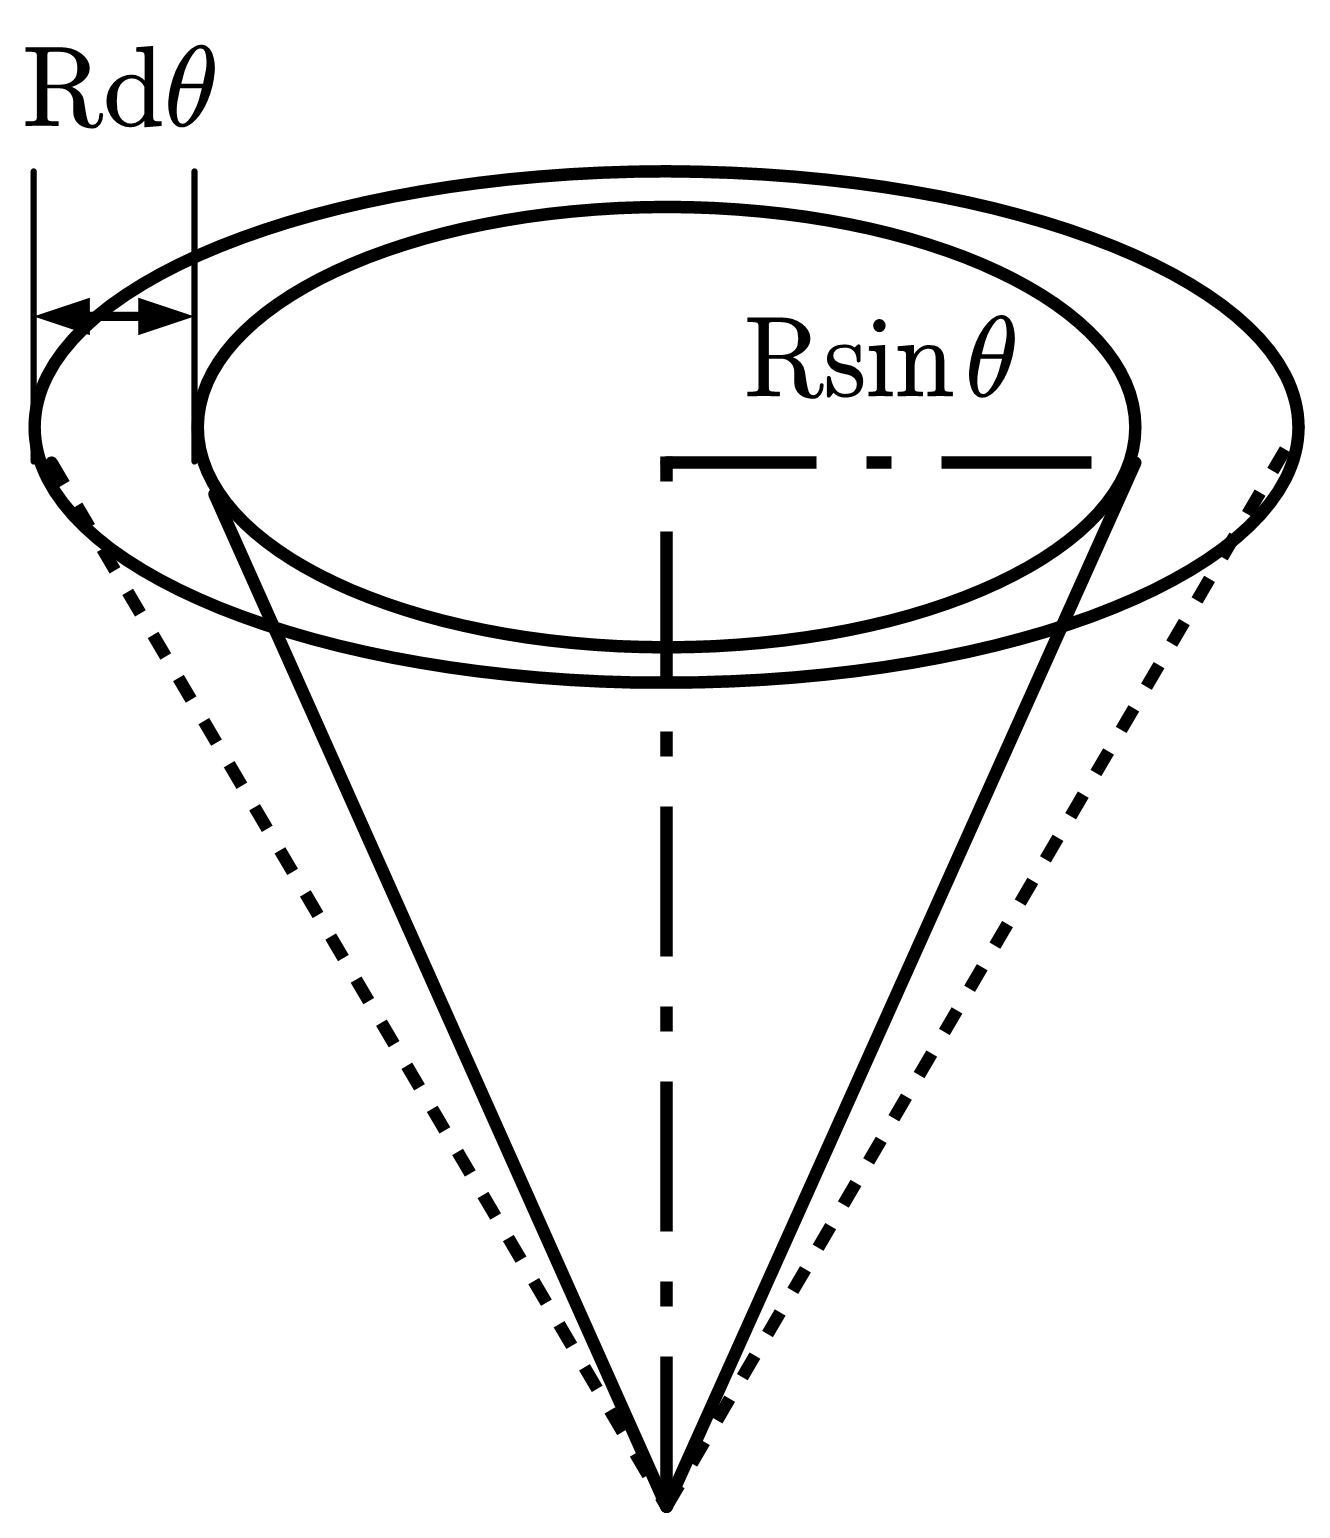
\includegraphics[width=4cm]{figure/NdThetaDist.png}
\end{center}
\subsubsection{常见情形下距离的分布}
\paragraph*{线段}在线段$[0,1]$上随机取2个点,计算距离的分布。

\begin{empheq}{align*}
\Prob(D\leq d)&=\Prob(|x-y|\leq d)\\
&=\Prob(x-d\leq y\leq x+d)
\end{empheq}

对应到正方形中对角梯形的面积,为
$$2\times \frac{\sqrt{2}+\sqrt{2}(1-d)}{2}\frac{d}{\sqrt{2}}=d(2-d)$$

\paragraph*{正方形}在矩形$[0,1]\times[0,1]$上随机取2个点,计算距离的分布。这个就非常复杂了。


\chapter{统计估计理论}\label{prob-stat-est}
\section{估计什么}
估计,可以是估计参数(参数估计理论),或者估计一个分布(贝叶斯分析,分类也是估计一个分布),或者估计某一个量(比如估计处理效应,这在概率论中有所分析.通常也与分布有关).

\paragraph*{估计某一个量} 给定一组样本$\{X_i\}_{i=1}^n,X_i\sim f(X_i;\theta)$,试估计$g(\theta)$。

在极大似然的框架下,可以首先通过极大似然估计$\theta$,然后直接计算$g(\theta)$。在贝叶斯框架下,需要估计的是$g(\theta;X)$,它是一个分布。

具体地说,假如是参数化模型,估计的量大致分为:
\begin{enumerate}
\item 只有确定型变量.通常就是最优化解决,如OLS.线性回归中的方差建模为确定型变量.
\item 定形随机变量.形是指形式、大小,比如线性回归中自变量的参数.可以用ML、EM估计.
\item 不定形随机变量.典型的例子是变分EM中的聚类个数.
\end{enumerate}
\section{估计中存在的问题}
各种扩展的统计模型大都是为了解决以下问题:

\begin{enumerate}
\item 噪声.当噪声为高斯时,比较好处理,非高斯就很难处理了.另外,噪声可能引起异常值,比如对一个分布进行采样,大概率会有一些值远超出平均水平,这是由概率的本性决定的.
\item 小样本.
\item 样本非独立或者非随机.我们希望样本是独立的,这样很容易拆开来分析;再者,相互作用属于非线性关系.但实践中不一定能做到随机采样,比如截断与删失(幸存者偏差也属于此类),有些样本没法观测到;又比如自相关,就是非独立.

非独立有两个维度,第一是纵向:个体间;第二是横向:变量间.潜变量模型也可以视为变量间非独立的例子.
\item 样本非同分布.只有样本本来属于同一个分布,才能通过许多样本对参数进行准确的估计,如果本来就不是同分布的,那么就难以准确地估计,因为不同样本的参数本来不一样.Mixture模型就是解决非同分布的一种方法,引入多个分布.

注意,非同分布有时不一定是一个问题,比如假如能找到驱动非同分布的变量,也可以放一起估计.从这里看,非同分布有时可能是选择的变量不完全.
\item 非线性,线性关系只有一种,而非线性关系则是无穷的.线性模型本质上相当于一阶展开式,它的一个特征时,参数在变量取不同值时的作用是一样的.
\item 分布不符合模型.通常我们是用噪声的分布指定模型的分布,所以分布不符合模型通常是说噪声分布不符合模型,比如非正态分布.
\end{enumerate}

\section{重要定义}
\subsection{估计量的性质}
\subsubsection{无偏性}
估计量的期望就是真实值:
$$\E(\hat{\btheta})=\btheta_o$$

\subsubsection{渐近一致}
$$\plim{n\rightarrow \infty} \hat{\btheta}=\btheta_o$$
实际相当于依概率收敛
\begin{equation}
\hat{\btheta}\xrightarrow{P}\btheta_o
\end{equation}

也可以表示为
$$\forall \varepsilon,\lim_{n\rightarrow \infty}\Prob\sbra{|\hat{\btheta}-\btheta_o|>\varepsilon}=0$$
另一个常见定义是样本趋于无穷大时,估计量极限为真实值,且方差为0.

注意依概率收敛弱于一致收敛:
\begin{equation}
\hat{\btheta}\xrightarrow{\text{a.s.}}\btheta_o
\end{equation}
或者
\begin{equation}
\Prob\left(\lim_{n\rightarrow \infty} \hat{\btheta}=\btheta_o\right)=1
\end{equation}
这里的意思是说概率全部集中在一点。

粗粗地看,渐近一致与无偏差不多,都描述了趋近于真实值的意思.但前者是静态的,只考虑期望,后者是动态的.一个估计量可以无偏但不渐近一致,也可以渐近一致但有偏.前者比较容易理解,只要方差没有趋于0,就没有渐近一致.

后者有点反直觉,给出一个例子:
$$\hat{\mu}=\frac{1}{N}+\frac{1}{N}\sum_{k=1}^Nx_i$$

这是有偏的,但方差是趋于0,因为常数的方差是0,加上常数不影响方差,而且样本无穷大时,前一项为0.
\subsubsection{相合估计量}

\subsubsection{无偏估计量的方差界限}
\paragraph*{Cramer Rao Bound}含义是在不同的$\theta_o$时,估计的难易程度不一样。

给定一组样本$X$,希望用它来估计$g(\theta)$,那么
$$\Var(\hat{g}(X))\geq \frac{\sdet{g'(\theta)}^2}{nI_1(\theta)}=\frac{\sdet{g'(\theta)}^2}{I(\theta)}$$
$I(\theta)$是Fisher信息矩阵\eqref{Fisher-Information},$I_1(\theta)$是单个样本的“贡献”。

如果$g(\theta)=\theta$,即直接估计$\theta$,那么有:
$$\Var(\hat{\theta})\geq \frac{1}{I(\theta)}$$

可见这个下界是与分布和参数有关的,而且注意这个下界并不总是能达到。这可以从推导过程看出来。

首先刻画无偏估计量:
\begin{empheq}{align*}
\int_x \sbra{\hat{\theta}-\theta}p(x|\theta)\dif x=0
\end{empheq}
上式中我们是用样本$x$估计参数,所以是对$x$积分。上式对$\theta$求导有:
\begin{empheq}{align*}
-\int_x p(x|\theta)\dif x+\int_x \sbra{\hat{\theta}-\theta}\frac{\partial p(x|\theta)}{\partial \theta}\dif x=0\\
\xRightarrow{} \int_x \sbra{\hat{\theta}-\theta}\frac{\partial \ln p(x|\theta)}{\partial \theta}p(x|\theta)\dif x=1
\end{empheq}
这个求导技巧在计算正态分布的方差时也使用了。

然后使用Schwaritx公式\eqref{int-Schwarz}估计方差:
$$\Var(\hat{\theta})=\int_x \sbra{\hat{\theta}-\theta}^2p(x|\theta)\dif x$$
\begin{empheq}{align*}
&\int_x\sbra{\hat{\theta}-\theta}^2p(x|\theta)\dif x \int_x \sbra{\frac{\partial \ln p(x|\theta)}{\partial \theta}}^2p(x|\theta)\dif x\\
\geq & \sbra{\int_x \sbra{\hat{\theta}-\theta}\sqrt{p(x|\theta)}\sbra{\frac{\partial \ln p(x|\theta)}{\partial \theta}}\sqrt{p(x|\theta)}\dif x}^2\\
=&1
\end{empheq}

比如对于正态分布
\begin{empheq}{align*}
I(\mu)&=nI_1(\theta)\\
&=-n\int_{\infty}^{\infty}\frac{\partial^2 \ln\phi(\frac{x-\mu}{\sigma})}{\partial^2 \mu}\phi\sbra{\frac{x-\mu}{\sigma}}\dif x\\
&=-n\int_{\infty}^{\infty}\frac{\partial^2 }{\partial^2 \mu}\sbra{-\frac{(x-\mu)^2}{2\sigma^2}}\phi\sbra{\frac{x-\mu}{\sigma}}\dif x\\
&=\frac{n}{\sigma^2}
\end{empheq}
假如$\sigma$非常小,接近0,那么只要1个样本,就基本可以确定$\mu$,反之,就很难确定。

现在用样本均值$\bar{X}$来估计$\mu$,则$\Var{\hat{\mu}}=\frac{\sigma^2}{n}$,即样本均值估计量到达了下界。

又比如,对于泊松分布,
\begin{empheq}{align*}
I(\lambda)&=-n\times \frac{1}{n}\sum_{n=0}^{\infty}\frac{\partial^2 }{\partial^2 \lambda}\sbra{C+n\ln \lambda-\lambda}p(n;\lambda)\\
&=-n\times \frac{1}{n}\sum_{n=0}^{\infty}\frac{-n }{\lambda^2}p(n;\lambda)\\
&=\frac{n}{\lambda^2}\sbra{\frac{1}{n}\sum_{n=0}^{\infty}np(n;\lambda)}\\
&=\frac{n}{\lambda}
\end{empheq}

样本均值$\bar{X}$估计量的方差是$\frac{\lambda}{n}$,也达到了下界。

对于chi-square分布
\begin{empheq}{align*}
I(\nu)&=-n\int_{\infty}^{\infty}\frac{\partial^2 \ln p(x;\nu)}{\partial^2 \nu}p(x;\nu)\dif x\\
&=-n\int_{\infty}^{\infty}\frac{\partial^2 \ln\sbra{-\ln\Gamma(\nu/2)+k\nu+C}}{\partial^2 \nu}p(x;\nu)\dif x\\
&=\frac{n}{4}\psi_1\sbra{\frac{\nu}{2}}
\end{empheq}
样本均值估计量的方差是$\frac{\nu}{n}$,它没有达到下界。


\subsection{Risk}
定义
$$\Risk(\hat{\beta})\coloneqq \E(L(\hat{\beta})-L(\beta))$$

对于LS,有
$$\Risk(\hat{\beta})=\E\|\hat{\beta}-\beta\|_\Sigma^2=\underbrace{\E\|\hat{\beta}-\bar{\beta}\|_\Sigma^2}_{\text{Variance}}+\underbrace{\|\bar{\beta}-\beta\|_\Sigma^2}_{\text{Prediction loss}}$$

其中$\Sigma=\frac{1}{n}X^TX,\|\bx\|_\Sigma=\bx^T\Sigma\bx$.
\section{估计方法概览}
\subsection{基于大数定律的估计}
估计方法大致上可以分为参数估计与非参数估计方法.参数估计预先假定一个数据的分布,并且分布完全由一组参数决定;而非参数估计不预先假定数据的分布,或者假定了分布,但分布并不由参数完全决定(比如高斯过程回归),又或者参数是无限维的.主要的非参模型有:

\begin{enumerate}
	\item 全部树方法.
	\item 核方法族.比如SVM、高斯过程回归.
	\item KNN.
\end{enumerate}

非参数模型通常与函数空间密切相关.比如给每条观测值分配一个函数,比如LOWESS,对每个点进行局部加权线性回归.


另外还有半参数方法,一部分由参数决定,另一部分不由参数决定,比如Mixture模型.

贝叶斯分析中的模型有参数模型,也有非参数模型.常见的贝叶斯回归模型均属于参数模型,比如贝叶斯线性回归.虽然贝叶斯分析把参数视为随机变量,但参数还是存在的,只不过取值是不确定的.有些贝叶斯模型的参数是无限维的,就认为它是非参数模型,比如狄利克雷回归.

所以贝叶斯分析与传统统计学的区别就是,传统统计学视参数为确定的,而贝叶斯分析视参数服从一个分布.

模型除了参数还有超参数,通常我们说的参数是指它决定了数据的分布,而超参数并不直接决定数据的分布.比如神经网络的学习率.又比如贝叶斯模型中先验分布的参数是属于超参数.

\subsection{基于小样本的估计}

\subsection{一些例子}
\subsubsection{用线性组合估计总体均值。}
\begin{example}
给定一个分布$N(\mu,1)$,现在有2个样本$X_1,X_2$。现在希望用两个样本的线性组合来估计$\mu$,即$\hat{\mu}=aX_1+bX_2$,问$a,b$在何种情况下可以得到最优的解。
\end{example}
\begin{solution}
给定$a,b$,则$\hat{\mu}$的分布是$N(a\mu+b\mu,a^2+b^2)$,此时$\mu$最有可能是$a\mu+b\mu$,立即可以得到$a+b=1$。然后此时的概率密度是$\frac{1}{\sqrt{2\pi}\sqrt{a^2+(1-a)^2}}$,最大化这个值,得到$a=b=\frac{1}{2}$。

第二种角度是从一致估计量的角度来考虑,由$\E(aX_1+bX_2)=\mu$,立即可以得到当$a+b=1$,同时计算$\Var(aX_1+bX_2)=(a^2+b^2)\Var(X)\geq \frac{1}{2}\Var(X)$,所以当$a=b=\frac{1}{2}$时,$\hat{\mu}$是方差最小的无偏估计量。

第三种角度是从极大似然考虑:$L=\phi(X_1-\hat{\mu})\phi(X_2-\hat{\mu})$,可以求出$\hat{\mu}=\frac{1}{2}(X_1+X_2)$。
	
这样其它我们得到了均值的最优估计。以上也相当于用一阶矩的最优估计。

\end{solution}
上面对于2个样本使用了极大似然估计,但实际上,只有在极少数情况下,小样本时的极大似然估计是无偏的。
\begin{example}
对于$\chi^2_v$分布,它的期望是$v$,对于2个样本,极大似然估计的情况如何?
\end{example}
\begin{solution}
在小样本时,$ML(\nu;X_1,X_2)\neq \frac{X_1+X_2}{2}$,但在大样本时
$$ML(v;X)\simeq \bar{X}$$。不仅如此,每次采样2个样本,得到$\hat{\nu_i}$的估计,重复$n$次,即便$\lim_{n\rightarrow \infty}\bar{\hat{\nu}}\neq \nu_o$,所以ML估计此时不是无偏的。

然而,即便在小样本时,样本均值仍然是$\nu$最小方差无偏线性估计量.那么对于非线性函数是否也是如此?这就是之前提到的Cramer Rao Bound,样本均值的方差没有达到下界。


\end{solution}
\section{参数估计——M估计}
M估计是一大类估计方法的统称,它通过极小化样本的某个泛函得到:

$$\sum_{k=1}^n \rho(\bm{\theta};\bm{x}_i,\bm{y}_i)$$

可以看出许多估计均属于此类.

\subsection{OLS估计}
\subsubsection{单因变量回归}
对于单一的自变量,系数为向量。OLS估计对应的泛函为

$$\rho(\bm{\theta};\bm{x}_i,y_i)=(y_i-\bm{x}_i^T\bm{\theta})^2$$

它的估计结果是:

\begin{empheq}{align*}
	\hat{\bm{\theta}}&=(X^TX)^{-1}X^T\bm{y}\\
	\Var(\hat{\bm{\theta}})&=(X^TX)^{-1}
\end{empheq}
\subsubsection{多因变量回归(向量回归)}
现在有多个因变量,则系数为一个矩阵:
$$\by=A\bx+\bm{e}$$

写成矩阵形式为:
$$Y=XA^T+E$$

注意$A$不必是一个方阵,如果取$\by_i\in\mathbb{R}^d,\bx_i\in\mathbb{R}^n$,则$A\in\mathbb{R}^{n\times d}$。仍然可以用OLS估计:
$$\rho(\bm{\theta};\bm{x}_i,\bm{y}_i)=\sum\trace\left((\bm{y}_i-\bm{x}_i^T\bm{\theta})^T(\bm{y}_i-\bm{x}_i^T\bm{\theta})\right)$$

在矩阵微分部分\ref{vector-regression-target}已经给出了上式的微分,因此可以求得
$$A=\left(\sum \by_i\bx_i^T\right)\left(\sum \bx_i\bx_i^T\right)^{-1}=Y^TX(X^TX)^{-1}$$
其中$Y_{N\times n},X_{N\times d}$.

\paragraph*{随机自变量}现在来考虑一个有意思的问题,假如$X$是一个随机生成的矩阵,即每一行为一个随机向量的值,且已知其协方差阵,问这种估计方法会得到什么。

首先$\E(X^TX)=N\Sigma_{\bm{x}}$,然后有
$$\E(A)=\bmu_{\by}\bmu_{\bx}^T\Sigma_{\bm{x}}^{-1}$$
注意到,假如两个均值向量有一个为0,则系数矩阵期望为零矩阵。于是残差矩阵为
$$E=Y-X\E(A)^T$$

\paragraph*{自变量为多向量}在向量自回归的模型,我们可能取高阶自回归项:
$$\by_i=A\by_{i-1}+B\by_{i-2}$$
其实可以把数据堆起来成为一个矩阵:
$$\by_i=\begin{bmatrix}
	A&B
\end{bmatrix}\begin{bmatrix}
\by_{i-1}\\\by_{i-2}
\end{bmatrix}$$
然后按之前的方法进行计算。

\subsubsection{加权LS}
为了解决异常值问题引入的方法.OLS中每条观测值对整体贡献是均等的,如果有异常值,就可能推高整体水平.那么一种自然的想法就是给高异常值的观测值分配一个权重.

$$\rho(\bm{\theta};\bm{x}_i,\bm{y}_i)=w_i(\bm{y}_i-\bm{x}_i^T\bm{\theta})^2$$

估计结果为:

\begin{empheq}{align*}
		\hat{\bm{\theta}}&=(X^TWX)^{-1}X^TW\bm{y}\\
		\hat{\Var(\bm{\theta})}&=(X^TWX)^{-1}
\end{empheq}

$W$是一个对角矩阵.

引入权重有许多种方式,最常见的是将$\bm{y}_i$的条件方差的倒数作为权重.这需要预先估计条件方差.一种做法是用一个另外的方程的残差方差作为条件方差,再对原方程进行估计.另一种做法是用本方程来估计条件方差并迭代改进系数(Iterated WLS).

以上是使用一组全局参数,假如对每个局部采用一小部分点进行加权回归,把各个局部拼起来形成整体,就是LOWESS回归,不过这是非参方法.神经网络的分层训练在思想上基本是一回事.
\subsection{工具变量估计}

\subsection{分位数回归}
\subsubsection{模型形式与求解}
OLS描述了变量对期望的影响,而分位数回归描述的是变量变动对分位数的影响,或者说预测值在回归线以下的比例.模型形式为

\begin{equation}\label{linear-qreg-model}
y_i^p=\alpha^p+A^p\bx_i+\epsilon_i^p
\end{equation}

$p$就表示小于$p$分位数的比例.

其距离函数是
\[
d(y,\hat{y})=\begin{cases}
(1-p)|y-\hat{y}|,&\text{ if }y\leq \hat{y}\\
p|y-\hat{y}|,&\text{ otherwise }
\end{cases}
\]

即拟合线以下的数据点权重为$(1-p)$.

整体的优化目标函数是
\begin{empheq}{align*}
\min L&=p\sum_{e_i\geq 0}|e_i|+(1-p)\sum_{e_i< 0}|e_i|\\
&=\sum_{i=0}^{n}e_i\left(pI(e_i\geq 0)+(p-1)I(e_i<0)\right)\\
&=\sum_{i=0}^n e_i(p-I(e_i<0))\\
e_i&=y_i-\hat{y}
\end{empheq}

以下展示用不同分位数进行估计得到的结果.
\begin{center}
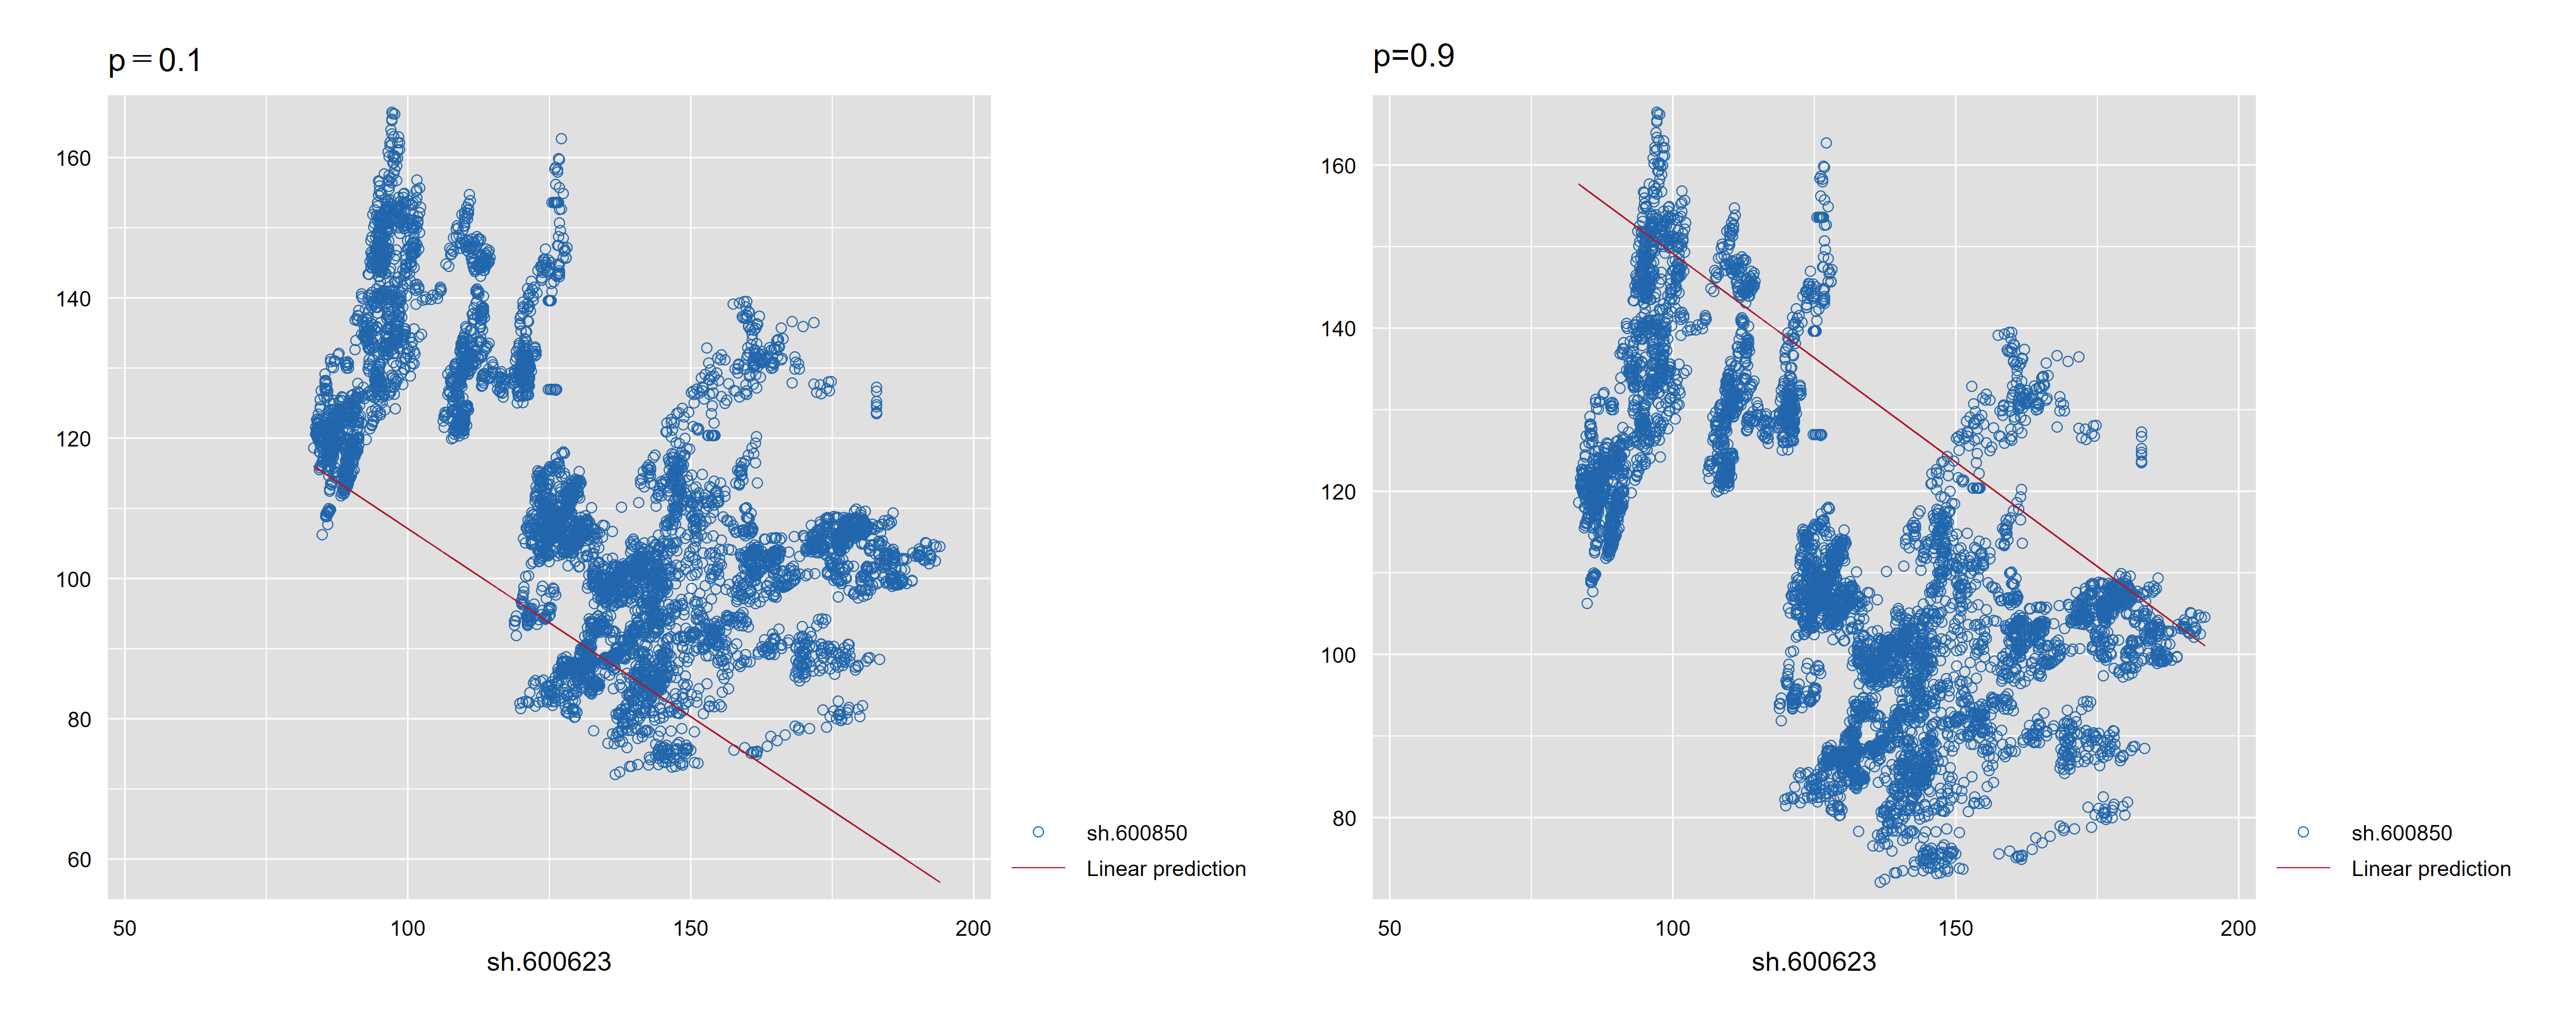
\includegraphics[width=\textwidth]{./figure/Qreg.png}
\end{center}

对于左边的图,有0.1比例的点在回归线以下,右边有0.9比例.所以分位数可以理解为
$$\E(y_i^p|\bx_i)$$

那么点在回归线以下的比例与分位数(注意每一个$\bx_i$对应一个分位数)有何关系呢?整体来看,有$p$比例的数在回归线以下,平均到每个点,就对应了每个$\bx_i$对应的分位数.反过来,$y_i^p$表示有$p$比例的$y_i$小于$y_i^p$,对应到整体就有$p$比例小于回归线.

而参数估计的置信区间就相当于进行多次分位数回归,即$y_i^{p}$的$(1-2\alpha)\%$置信区间是:
$$\left[y_i^{p_1},y_i^{p_2}\right]$$
$$p_2-p_1=1-2\alpha$$

注意这个置信区间与$p$没有直接关系.相当于说分位数的置信区间还是分位数.

由于VaR也是描述了分位数,所以一个很自然的应用就是用分位数回归计算VaR.
\subsubsection{分位数回归的优点}
\begin{enumerate}
\item 不需要假定残差的分布,适合处理非正态分布、异方差.
\item 通过对残差加权可以降低异常值的影响,另一方面,我们只看比例,那么就算异常值超出很多也关系不大,这也说明不易受异常值影响.
\item 可以设定不同的$p$拟合多条曲线.对于高斯模型,假如是异方差,则不同曲线斜率不同;同方差时,斜率是相同的.这很好理解,假如是同方差,则增大$p$时,各个$\bx_i$对应的预测值应当增加得比较均匀.

由不同的斜率可以诱导变量对不同分位数的影响,那么现实中就可以用来度量某些因素对不同收入人群的影响.
\end{enumerate}

\subsubsection{扩展}
\paragraph*{神经网络分位数回归}在\eqref{linear-qreg-model}的模型中,如果用神经网络来输出结果$\hat{y}$,就得到神经网络分位数回归。

\subsection{极大似然估计}
\subsubsection{计算}
$$\rho(\bm{\theta};\bm{x}_i,\bm{y}_i)=-\ln f(\bm{\theta};\bm{x}_i,\bm{y}_i)$$

$f$表示概率密度.

MLE估计中的一个重要度量是Fisher信息.对于单变量,定义为:
\begin{empheq}{align}
\mathcal{I}(\theta)&=E_{f(X;\theta)}\left[ \sbra{\frac{\partial \ln f(X;\theta)}{\partial \theta}}^2 \right]=-E_{f(X;\theta)}\left[\frac{\partial^2 \ln f(X;\theta)}{\partial \theta^2}\right]\mtag{Fisher Information} \label{Fisher-Information}
\end{empheq}

显然第二个等号需要函数是二次可微的,但这并不总是成立。由第一个等号可知,这个值总是大于0的。

含义是,任意无偏估计的方差不能小于这个值,所以它给出了无偏估计方差的下界.但有偏的时候,方差是可以小于这个下界的.注意,求$I(\theta)$时由于对$X$进行积分,所以并没有涉及真实的样本,而且这个值与分布和参数有关。

对于多变量,定义:
\begin{empheq}{align*}
 \mathcal{I}(\bm{\theta})&=E\left[\nabla \ln f\nabla^T \ln f|\theta\right]^2=-E\left[\textbf{H}( \ln f) | \theta\right]
\end{empheq}

\textbf{H}表示Hessian矩阵.
\subsubsection{极大似然估计的一致性}
极大似然估计是最大化:
$$\frac{1}{n}\sum_{i=1}^{N}\ln f(X_i|\theta)$$
根据大数定律,在样本无穷大时
$$\frac{1}{n}\sum_{i=1}^{N}\ln f(X_i|\theta)\rightarrow \E_{\theta_o}\ssbra{\ln f(X|\theta)}$$
最优化左边,就相当于最优化右边。右边最优化,那就是$\theta_o$。现在证明右边确实在$\theta_o$处取得最大值:
\begin{empheq}{align*}
\E_{\theta_o}\ssbra{\ln f(X|\theta)}-\E_{\theta_o}\ssbra{\ln f(X|\theta_o)}&=\E_{\theta_o}\ssbra{\ln\frac{f(X|\theta)}{f(X|\theta_o)}}\\
&\leq \ln \E_{\theta_o}\ssbra{\frac{f(X|\theta)}{f(X|\theta_o)}}\\
&=\ln \int\frac{f(x|\theta)}{f(x|\theta_o)}f(x|\theta_o)\dif x\\
&=0
\end{empheq}
当然,这个值不一定是唯一的。

\subsubsection{实例}
\paragraph*{高斯分布多元线性回归}模型为
$$\by=\bx_i^T\theta+e_i,\quad e\sim \mathcal{N}(0,\sigma^2)$$

似然函数为
$$LL(\bx_i;\btheta,\sigma^2)=\text{const}-\inv{2}\ln \sigma^2 -\frac{1}{\sigma^2}(y_i-\bx_i^T\btheta)^2$$

根据Robbins-Monro\label{Robbins-Monro}方法,导出一个Online算法:
\begin{empheq}{align}
\btheta_{i+1}&=\btheta_i+\eta (y_i-\bx_i^T\btheta_i)\bx_i=\btheta_i+\eta e_i\bx_i\label{single-var-gaussian-reg-theta}\\
\sigma_{i+1}^2&=(1-\eta)\sigma_i^2+\eta e_i^2\label{gauss-linear-reg-sigma2-online}
\end{empheq}
$\btheta_0$一般初始化为$\bm{0}$。

式\eqref{single-var-gaussian-reg-theta}中没有用到$\sigma$,可以理解为是用MSE的损失函数来推导的,如果严格按照MLE的损失函数来推导,应该是
\begin{empheq}{equation}\label{single-var-gaussian-reg-theta-no-sigma}
\btheta_{i+1}=\btheta_i+\eta \frac{e_i}{\sigma^2}\bx_i
\end{empheq}

这两个更新公式在动力学上是肯定不一样的。但最终结果却是相似的。可以这样来分析,假设初始为$\btheta^{(0)}$,用所有数据进行一次性更新(Full batch)后为$\btheta^{(1)}$。则式\cref{single-var-gaussian-reg-theta, single-var-gaussian-reg-theta-no-sigma}的更新过程分别对应为:
\begin{empheq}{align}
\btheta^{(k+1)}&=\btheta^{(k)}+\eta \sum_{i=1} (y_i-\bx_i^T\btheta^{(k)})\bx_i\\
\btheta^{(k+1)}&=\btheta^{(k)}+\eta\sum_{i=1} \frac{1}{\sigma^2}(y_i-\bx_i^T\btheta^{(k)})e_i^T\bx_i
\end{empheq}
可以理解为不动点迭代,则两式的不动点分别为:
\begin{empheq}{align}\label{single-var-gaussian-reg-theta-fixed-point}
\sum_{i=1}(y_i-\bx_i^T\btheta^{(k)})\bx_i&=0\\
\sum_{i=1}\frac{1}{\sigma^2}(y_i-\bx_i^T\btheta^{(k)})e_i^T\bx_i&=0 
\end{empheq}
显然,不动点是一样的。不过这里是假定$\sigma$为常量,实际上由于在线算法是每次用一条样本更新一次,此时不动点不再由方程\eqref{single-var-gaussian-reg-theta-fixed-point}直接给出,因此最终结果会有微小差异。

$\sigma^2$的迭代公式是这样给出的:首先计算梯度$\pdv{LL}{\sigma^2}=-\inv{2}\inv{\sigma^2}+\inv{2}e_i^2\inv{(\sigma_n^2)^2}$,直接写出的迭代公式为:
$$\sigma_{i+1}^2=\sigma_{i}^2+\eta\left(e_i^2\inv{(\sigma_i^2)^2}-\inv{\sigma_i^2}\right)$$
上式两边乘以$(\sigma_i^2)^2$有:
$$\sigma_{i+1}^2(\sigma_i^2)^2=(\sigma_i^2)^3+\eta(e_i^2-\sigma_i^2)$$
稳态时$\sigma_{i+1}^2(\sigma_i^2)^2=(\sigma_i^2)^3$,消去这两项,再在左边加上$\sigma_{i+1}^2$,右边加上$\sigma_i^2$,即可得到式\eqref{gauss-linear-reg-sigma2-online}。

\paragraph*{高斯分布向量回归}模型为
$$\by_i=A\bx_i+\bm{e}_i,\bm{e}_i\sim\mathcal{N}(\bm{0},\Sigma)$$

单样本似然函数为
$$LL(\bx_i;A,\Sigma)=-\frac{d}{2}\ln(2\pi)-\inv{2}\ln|\Sigma|-\inv{2}\bm{e}_i^T\Sigma^{-1}\bm{e}_i$$

正则方程组为
\begin{empheq}{align}
\pdv{LL}{A}&=\sum_{i=1}^{N}\Sigma^{-1}(\by_i-A\bx_i)\bx_i^T=0\\
\pdv{LL}{\Sigma^{-1}}&=\frac{N}{2}\Sigma-\inv{2}\sum_{i=1}^{N}\bm{e}_i\bm{e}_i^T=0
\end{empheq}
解为:
\begin{empheq}{align}
A&=\left(\sum_{i=1}^{N}\by_i\bx_i^T\right)\left(\sum_{i=1}^{N}\bx_i\bx_i^T\right)^{-1}=Y^TX(X^TX)^{-1}\\
\Sigma&=\inv{N}\sum_{i=1}^{N}\bm{e}_i\bm{e}_i^T=\inv{N}(Y-XA^T)^T(Y-XA^T)
\end{empheq}
式中$Y\in \mathbb{R}^{n\times d}$,为将$\by_i^T$按行堆积后形成的矩阵。同样的结果用OLS估计也可以得到。

同时导出Robbins-Monro类Online算法:
\begin{empheq}{align}
A_{i+1}&=A_i+\eta \bm{e}_i\bx_i^T \label{mv-gaussian-reg-A}\\
\Sigma_{i+1}&=(1-\eta)\Sigma_i+\eta \bm{e}_i\bm{e}_i^T\\
\Sigma_{i+1}^{-1}&=\Sigma_{i}^{-1}+\eta (\Sigma_i-\bm{e}_i\bm{e}_i^T)
\end{empheq}

\paragraph*{t分布多元线性回归}形式与高斯多元线性回归相同,只是分布假设不一样,由于t分布的长尾特性,适合进行Robust回归。
$$y_i=\bx_i^T\theta+e_i,\quad e\sim t_{\nu}(0,\sigma^2)$$
$\nu$一般可以固定为3,作为参数来学习也是可以的。

对数似然函数为
$$LL=\ln\Gamma\left(\frac{\nu+1}{2}\right)-\ln\Gamma\left(\frac{\nu}{2}\right)-\inv{2}\ln(\nu\pi)-\inv{2}\ln\sigma^2-\frac{\nu+1}{2}\ln\left(1+\inv{\nu}\left(\frac{(y_i-\bx_i^T\btheta)^2}{\sigma^2}\right)\right)$$

首先求出梯度:
\begin{empheq}{align*}
\alpha_i&=\frac{\nu+1}{\nu+e_i^2/\sigma^2}\\
\pdv{LL}{\btheta}&=\alpha_i\inv{\sigma^2}e_i\bx_i\\
\pdv{LL}{\sigma^2}&=\inv{2}\left(-\inv{\sigma^2}+\alpha_i\frac{e_i^2}{(\sigma^2)^2}\right)\\
\pdv{LL}{\nu}&=\inv{2}\left(\psi\left(\frac{\nu+1}{2}\right)-\psi\left(\frac{\nu}{2}\right)-\inv{\nu}-\ln\left(1+\inv{\nu}\left(\frac{e_i^2}{\sigma^2}\right)\right)+\alpha_i\frac{e_i^2}{\sigma^2}\inv{\nu}\right)
\end{empheq}
上式中$\psi(x)$为特殊函数\ref{digamma}。从以上也可以看出t分布回归与高斯分布回归的关系,当$\nu\rightarrow\infty$时,$\alpha_i\rightarrow 1$,则更新过程趋于高斯分布回归。

$\btheta,\nu$的更新公式立即可得,不过$\sigma^2$的更新公式可以进行一下变换:
\begin{empheq}{align*}
\sigma_{n+1}^2&=\sigma_n^2+\eta \frac{e_i^2-\sigma^2}{e_i^2+\nu\sigma^2}
\end{empheq}

另一方面可以重参数化,更新$\inv{\sigma^2}$,导数为:
$$\pdv{LL}{(\sigma^2)^{-1}}=\inv{2}\sigma^2-\inv{2}\frac{\nu+1}{\nu+e_i^2(\sigma^2)^{-1}}e_i^2$$
得到更新公式为:
$$\sigma_{n+1}^{-2}=\sigma_{n}^{-2}+\eta\left(1/\sigma_{n}^{-2}-\alpha_ie_i^2\right)$$

由于t分布的长尾特性,可以猜测使用$t$分布回归得到的$\sigma^2_{\text{t}}<\sigma^2_{\text{Gaussian}}$,因为前者会“忽略”一些异常值。

\paragraph*{t分布向量线性回归}模型为
$$\by_i=A\bx_i+\bm{e}_i,\bm{e}_i\sim t_{\nu}(\bm{0},\Sigma),A\in\mathbb{R}^{d\times k},\bx_i\in\mathbb{R}^d,\by\in\mathbb{R}^n$$

对数似然函数为:
\begin{empheq}{align}
LL(\bx_i;A,\nu,\Sigma)=\ln\Gamma\left(\frac{\nu+d}{2}\right)-\ln\Gamma\left(\frac{\nu}{2}\right)-\frac{d}{2}\ln(\nu\pi)-\inv{2}\ln|\Sigma|-\frac{\nu+d}{2}\ln\left(1+\inv{\nu}\bm{e}_i^T\Sigma^{-1}\bm{e}_i\right)
\end{empheq}

导数为:
\begin{empheq}{align}
\alpha_i&=\frac{\nu+d}{\nu+\bm{e}_i^T\Sigma^{-1}\bm{e}_i}\\
\pdv{LL}{A}&=\alpha_i\Sigma^{-1}\bm{e}_i\bx_i^T\\
\pdv{LL}{\Sigma}&=\inv{2}(-\Sigma^{-1}+\alpha(\Sigma^{-1}\bm{e})(\Sigma^{-1}\bm{e})^T)=\inv{2}(-\Sigma^{-1}+\alpha\Sigma^{-1}(\bm{e}\bm{e})^T\Sigma^{-1})\\
\pdv{LL}{\Sigma^{-1}}&=\inv{2}\left(\Sigma-\alpha\bm{e}_i\bm{e}_i^T\right)\\
\pdv{LL}{\nu}&=\inv{2}\left(\psi\left(\frac{\nu+d}{2}\right)-\psi\left(\frac{\nu}{2}\right)-\frac{d}{\nu}-\ln\left(1+\inv{\nu}\bm{e}_i^T\Sigma^{-1}\bm{e}_i\right)+\alpha_i \frac{\bm{e}_i^T\Sigma^{-1}\bm{e}_i}{\nu}\right)
\end{empheq}

实践中看,如果使用在线算法,那更新$\Sigma,\Sigma^{-1}$效果差别不明显,不过后者的复杂度稍低,收敛速度稍快。此外如果更新$\Sigma^{-1}$,那么$\det$那一项应该是$+\inv{2}\ln|\Sigma^{-1}|$,不要搞错前面的符号。步长要足够小,大概$10^{-3}$不错。
\subsection{矩估计}

\section{参数估计——贝叶斯估计}
\subsection{后验分布的计算}
\subsubsection{线性回归}
线性回归$\by=X\btheta+\bmeta,\btheta\sim \mathcal{N}(\bmu_{\btheta},\Sigma_{\btheta}),\btheta\in\mathbb{R}^{k\times 1},\bmeta\in\mathbb{R}^{n\times 1}$,注意,一般的线性回归中是假设$\btheta$不为随机变量。则分布
\begin{empheq}{align}
p(\btheta)&=\mathcal{N}\sbra{\btheta-\bmu_{\btheta},\Sigma_{\btheta}}\\
p(\by)&=\mathcal{N}(\by-X\bmu_{\btheta},\Sigma_{\bmeta}+X\Sigma_{\btheta}X^T)\\
p(\by|\btheta)&=\mathcal{N}(\by-X\btheta,\Sigma_{\bmeta})
\end{empheq}
后验分布
\begin{empheq}{align}\label{linear-gauss-posterior}
p(\btheta|\by)&=\mathcal{N}(\btheta-\bmu_{\btheta|\by},\Sigma_{\btheta|\by})\\
\bmu_{\btheta|\by}&=\bmu_{\btheta}+\left(\Sigma_{\btheta}^{-1}+X^T\Sigma_{\bmeta}^{-1}X\right)^{-1}X^T\Sigma_{\bmeta}^{-1}(\by-X\bmu_{\btheta})\\
\Sigma_{\btheta|\by}&=\left(\Sigma_{\btheta}^{-1}+X^T\Sigma_{\bmeta}^{-1}X\right)^{-1}
\end{empheq}

这个后验分布非常难算,最直接的办法就是用贝叶斯公式强行计算:
\begin{empheq}{align*}
p(\btheta|\by)&=\frac{p(\by|\btheta)p(\btheta)}{p(\by)}\\
\end{empheq}
完整展开如下:
\begin{empheq}{align*}
&(2\pi)^{-\frac{n}{2}}\left|\Sigma_{\bmeta}\right|^{-\frac{1}{2}}\exp\left(-\frac{1}{2}(\by-X\btheta)^T\Sigma_{\bmeta}^{-1}(\by-X\btheta)\right)\\
\times & (2\pi)^{-\frac{k}{2}}\left|\Sigma_{\btheta}\right|^{-\frac{1}{2}}\exp\left(-\frac{1}{2}\sbra{\btheta-\bmu_{\btheta}}^T\Sigma_{\btheta}^{-1}\sbra{\btheta-\bmu_{\btheta}}\right)\\
\hline &(2\pi)^{-\frac{n}{2}}\left|\Sigma_{\bmeta}+X\Sigma_{\btheta}X^T\right|^{-\frac{1}{2}}\exp\left(-\frac{1}{2}(y-X\bmu_{\btheta})^T\left(\Sigma_{\bmeta}+X\Sigma_{\btheta}X^T\right)^{-1}(y-X\bmu_{\btheta})\right)
\end{empheq}
可以看出这个后验分布显然还是高斯分布,因为指数项是二次的。上式中常数项可以约掉$n$的指数。然后考虑$\det$项。
\begin{empheq}{align*}
\frac{\left|\Sigma_{\bmeta}\right|^{-\frac{1}{2}}\left|\Sigma_{\btheta}\right|^{-\frac{1}{2}}}{\left|\Sigma_{\bmeta}+X\Sigma_{\btheta}X^T\right|^{-\frac{1}{2}}}&=\left|\Sigma_{\btheta}\right|^{-\frac{1}{2}}\left|\Sigma_{\bmeta}\left(\Sigma_{\bmeta}+X\Sigma_{\btheta}X^T\right)^{-1}\right|^{-\frac{1}{2}}\\
&=\left|\Sigma_{\btheta}\right|^{-\frac{1}{2}}\left|\left(I_n+\Sigma_{\bmeta}^{-1}X\Sigma_{\btheta}X^T\right)^{-1}\right|^{-\frac{1}{2}}\\
\underline{\sdet{I_n+AB^T}=\sdet{I_k+A^TB}}&=\left|\Sigma_{\btheta}\right|^{-\frac{1}{2}}\sdet{\left(I_k+X^T\Sigma_{\bmeta}^{-1}X\Sigma_{\btheta}\right)^{-1}}^{-\frac{1}{2}}\\
\underline{\sdet{A^{-1}+A^{-1}BA}=\sdet{A^{-1}+B}}&=\sdet{\sbra{\Sigma_{\btheta}^{-1}+\Sigma_{\btheta}^{-1}X^T\Sigma_{\bmeta}^{-1}X\Sigma_{\btheta}}^{-1}}^{-\frac{1}{2}}\\
&=\sdet{\sbra{\Sigma_{\btheta}^{-1}+X^T\Sigma_{\bmeta}^{-1}X}^{-1}}^{-\frac{1}{2}}
\end{empheq}

其实这里已经求出了条件分布的协方差阵。现在来考虑指数项,省略前面的$-\frac{1}{2}$:
\begin{empheq}{align*}
&\sbra{\by-X\btheta}^T\Sigma_{\bmeta}^{-1}\sbra{\by-X\btheta}+\sbra{\btheta-\bmu_{\btheta}}^T\Sigma_{\btheta}^{-1}\sbra{\btheta-\bmu_{\btheta}}-(y-X\bmu_{\btheta})^T\left(\Sigma_{\bmeta}+X\Sigma_{\btheta}X^T\right)^{-1}(y-X\bmu_{\btheta})\\
=&\sbra{\by-X\btheta}^T\Sigma_{\bmeta}^{-1}\sbra{\by-X\btheta}+\sbra{\btheta-\bmu_{\btheta}}^T\Sigma_{\btheta}^{-1}\sbra{\btheta-\bmu_{\btheta}}\\
&-(y-X\bmu_{\btheta})^T\left(\Sigma_{\bmeta}^{-1}-\Sigma_{\bmeta}^{-1}X\left(\Sigma_{\btheta}^{-1}+X^T\Sigma_{\bmeta}^{-1}X\right)^{-1}X^T\Sigma_{\bmeta}^{-1}\right)^{-1}(y-X\bmu_{\btheta})\\
=&\sbra{\by-X\btheta}^T\Sigma_{\bmeta}^{-1}\sbra{\by-X\btheta}+\sbra{\btheta-\bmu_{\btheta}}^T\Sigma_{\btheta}^{-1}\sbra{\btheta-\bmu_{\btheta}}-(y-X\bmu_{\btheta})^T\Sigma_{\bmeta}^{-1}(y-X\bmu_{\btheta})\\
&+\uwave{(y-X\bmu_{\btheta})^T\Sigma_{\bmeta}^{-1}X\sbra{\Sigma_{\btheta}^{-1}+X^T\Sigma_{\bmeta}^{-1}X}^{-1}}\underline{\sbra{\Sigma_{\btheta}^{-1}+X^T\Sigma_{\bmeta}^{-1}X}}\uwave{\sbra{\Sigma_{\btheta}^{-1}+X^T\Sigma_{\bmeta}^{-1}X}^{-1}X^T\Sigma_{\bmeta}^{-1}(y-X\bmu_{\btheta})}
\end{empheq}

上式的第二部分是显面易见的二次型,现在只需要考虑第一部分。基本思路是把第一部分的第一项拆开,再与第三项组合,第一部分
\begin{empheq}{align*}
&\sbra{y-X\bmu_{\btheta}+X\bmu_{\btheta}-X\btheta}^T\Sigma_{\bmeta}^{-1}\sbra{y-X\bmu_{\btheta}+X\bmu_{\btheta}-X\btheta}+\sbra{\bmu_{\btheta}-\btheta}^T\Sigma_{\btheta}^{-1}\sbra{\bmu_{\btheta}-\btheta}-(y-X\bmu_{\btheta})^T\Sigma_{\bmeta}^{-1}(y-X\bmu_{\btheta})\\
=&\sbra{\bmu_{\btheta}-\btheta}^T\underline{\sbra{\Sigma_{\btheta}^{-1}+X^T\Sigma_{\bmeta}^{-1}X}}\sbra{\bmu_{\btheta}-\btheta}+2\sbra{y-X\bmu_{\btheta}}^T\Sigma_{\bmeta}^{-1}X(\bmu_{\btheta}-\btheta)\\
=&\sbra{\bmu_{\btheta}-\btheta}^T\underline{\sbra{\Sigma_{\btheta}^{-1}+X^T\Sigma_{\bmeta}^{-1}X}}\sbra{\bmu_{\btheta}-\btheta}\\
&+2\uwave{\sbra{y-X\bmu_{\btheta}}^T\Sigma_{\bmeta}^{-1}X\sbra{\Sigma_{\btheta}^{-1}+X^T\Sigma_{\bmeta}^{-1}X}^{-1}}\underline{\sbra{\Sigma_{\btheta}^{-1}+X^T\Sigma_{\bmeta}^{-1}X}}\sbra{\bmu_{\btheta}-\btheta}
\end{empheq}
再与原来的第二部分合并起来看,二次型已经非常明显了。

\section{随机逼近理论}
\subsection{Robbins-Monro方法}\label{Robbins-Monro}
假设我们希望求解
$$f(\btheta)=\E(\phi(\btheta,\bbeta))$$
的零点,其中$\eta$为未知的统计量,假设它是已知的,则可以用一般的解方程组方法求解。在未知的情况下,$f$的具体形式是不知道的。Robbins-Monro方法就是给定一组独立同分布的观测值$\bbeta_0,\bbeta_1,\cdots$,按如下更新$\btheta$:
\begin{empheq}{equation}
\btheta_n=\btheta_{n-1}-\mu_n\phi(\btheta_{n-1},\bbeta_n),\sum \mu_n^2<\infty, \sum \mu_n\rightarrow \infty
\end{empheq}
从迭代过程可以看出,它适宜用来导出在线算法。

在这个算法中,假如取$\phi$为梯度,则可以得到梯度下降法:
$$\btheta_n=\btheta_{n-1}-\nabla \mathcal{L}(\btheta_{n-1},y_n\bx_n)$$

在线性回归中,我们希望求解:
$$\E(\bx(\bx^T\btheta-y))=0$$
使用Robbins-Monro方法即有:
\begin{empheq}{equation}
\btheta_n=\btheta_{n-1}+\mu_n\bx_n\bm{e}_n=\btheta_{n-1}+\mu_n\bx_n(y_n-\bx_n^T\btheta_{n-1})\mtag{LMS算法}
\end{empheq}

\section{正则化}
正则化往往与约束有关,比如稀疏化:将某些参数归0.正则化的一个好处是减少了参数数量,容易训练模型;防止过拟合,增强泛化能力.

\subsection{岭回归}\label{Tikhonov-regularization}
Ridge Regression,又叫Tikhonov正则化.参数估计如下:
\begin{empheq}{align}
\hat{\bbeta}&=\argmin_{\btheta} \|\by-X\btheta\|+\lambda \|\btheta\|^2\\
&=\left(\Sigma+\lambda I\right)^{-1}\left(\frac{1}{N}X^T\by\right)
\end{empheq}

其中$\Sigma=\frac{1}{N}X^TX$.

\section{EM方法}
\subsection{基本过程}
EM方法常用于包含潜变量的模型估计,记$\chi^l$为(随机)潜变量,$\xi$为确定型的超参数,基本过程如下:
\begin{enumerate}
\item Expectation:计算$p(\chi^l|\chi,\xi^{(j)})$以及
$$\mathcal{Q}(\xi,\xi^{(j)})\coloneqq \E\left(\ln p(\chi^l,\chi;\xi)\right)=\E(\ln p(\chi|\chi^l)+\ln p(\chi^l))$$
期望是针对$p(\chi^l|\chi,\theta^{(j)})$求的.如果使用高斯分布,则后验也是高斯分布,容易计算.同时可以看出,EM方法需要计算潜变量的条件分布,如果难以计算,则EM方法就不能进行.

此外,对于上式最右边,期望中第一项相当于ML估计的似然函数,第二项相当于潜变量的似然函数。

\item Maximization:最优化求解$\xi^{(j+1)}$,
$$\xi^{(j+1)}=\argmax_{\xi} \mathcal{Q}(\xi,\xi^{(j)})$$
\end{enumerate}

这个算法看起来比较简单,但比较难以理解.以下给出一些例子.

\subsection{EM线性回归}
考虑线性回归$\by=X\btheta+\bmeta,X\in \mathbb{R}^{n\times k}$,潜变量为$\btheta$,参数$\bxi$与协方差有关:$\Sigma_{\bmeta}=\sigma_{\bmeta}^2I,\Sigma_{\btheta}=\sigma_{\btheta}^2I,\bxi=[\alpha,\beta],\alpha=\frac{1}{\sigma_{\btheta}^2},\beta=\frac{1}{\sigma_{\bmeta}^2}$,这里其实假定了参数分布为正态分布.

\paragraph*{E-Step}似然函数
$$\ln p(\by|\btheta;\bxi)=n\ln \frac{1}{2\pi}+\frac{n}{2}\ln\beta-\frac{\beta}{2}\|\by-X\btheta\|^2$$

潜变量似然函数
$$\ln p(\btheta;\bxi)=k\ln \frac{1}{2\pi}+\frac{k}{2}\ln\alpha-\frac{\alpha}{2}\btheta^T\btheta$$

求期望时,要用到后验分布,参考\eqref{linear-gauss-posterior}。


\paragraph*{M-Step}

\subsection{EM-GMM}
GMM是指Gauss Mixture Model.区分它与FMM(Finite Mixture Model),前者只用于分类,后者有分类,还有回归。

\section{变分推断}
变分推断在不同的地方有不同的说法.有人认为变分推断可以推导出EM。

\subsection{基本原理}
参数估计是通过优化某个目标函数(比如似然函数、MSE)来得到估计结果,而非参估计一般是通过采样或者其它一些方法。变分推断也是使用优化的方法,其目标函数是ELBO,由KL散度导出。

那么它是针对什么来进行优化的?在变分推断中,我们对潜变量的分布进行假设,得到其分布形式和参数,然后通过优化找到最优的参数。常见的一种分布形式就是平均场近似,它是假设参数间的分布是独立的。

记$\bz$为潜变量,我们希望得到后验分布
$$p(\bz|\bx)=\frac{p(\bx|\bz)p(\bz)}{p(\bx)}$$
但$p(\bx)$通常是很难得到的。在变分推断中我们转而求解
$$q^\star(\bz)=\argmin_{\btheta}\text{KL}(q(\bz;\btheta))\|p(\bz|\bx)$$
即寻找一个最接近目标后验分布的分布。显然,“变分”的名字就是从这里来的,我们是把$q$当作一个函数来优化。

现在有
\begin{empheq}{align}
\text{KL}(q(\bz;\btheta))\|p(\bz|\bx)&=\E\left(\ln(p(\bz))\right)-\E\left(\ln(p(\bz|\bx))\right)\\
&=\E\left(\ln(p(\bz))\right)-\E\left(\ln(p(\bz,\bx))\right)+\ln(p(\bx))
\end{empheq}
记
\begin{empheq}{equation}\label{ELBO}
\text{ELBO}(q)=\E\left(\ln(p(\bz,\bx))\right)-\E\left(\ln(p(\bz))\right)\mtag{ELBO}
\end{empheq}
由于$p(\bx)$是常数,那么最大化ELBO,相当于最小化KL。同时可以看出
$$\ln(p(\bx))=\KL\left(q(\bz)\|p(\bz|\bx)\right)+\text{ELBO}(q)$$
由于KL必然大于等于0,因此ELBO可以作为$p(\bx)$的下界。

对ELBO进行一些变换可以得到
\begin{empheq}{align}
\text{ELBO}(q)&=\E\left(\ln(p(\bz))\right)+\E\left(\ln(p(\bx|\bz))\right)-\E\left(\ln(p(\bz))\right)\\
&=\E\left(\ln(p(\bx|\bz))\right)-\KL(q(\bz)\|p(\bz))
\end{empheq}
\subsection{平均场逼近与循环上升}
假设潜变量之间的独立的,那么有
$$q(\bz)=\prod_{k=1}^{n}q_k(z_k)$$

使用类似于EM的思想,由于子分布间是独立的,那么可以循环优化每个分量。假设除了$q_k$,其它参数都知道了,那么有
$$\ln q_k(z_k)\propto \E_{-k}\left(\ln p(z_k|\bz_{-k},x\right)$$

问题在于$p\left(z_k|\bz_{-k},x\right)$如何计算?通常这是由模型决定的。$\ln p$是$z_k,\bz_{-k}$的函数,取期望后是$z_k, \E(\bz_{-k})$的函数,后者是矩量。假如右边是一个二次项,那么取指数就得到$q_k$是正态分布。所以我们并不假设$q_k$的具体形式,具体形式是通过计算导出的。

而且实际上我们并不需要$q_k$的具体形式,因为在更新其它分布时,通常只需要得到矩量就可以了,即最终需要的是诸如$\E(q_k(z_k))$之类的矩量。不过通过右边的形式导出$q_k$的分布形式,可以便于计算,否则要进行积分,也很麻烦。

\subsection{变分EM}

\subsection{神经网络中的变分推理}

\section{非参方法}
\subsection{核函数}
\subsubsection{基本含义}
简单地说,核函数就是计算两个点在高维投影下的内积。假如没有核函数,那么我们先要把点投影到高维空间,得到高维向量,再对高维向量计算内和。但很多情况下,我们只需要这个内积就够了,并不需要点的高维投影的具体表示。核函数就可以完成这个任务:在低维空间中计算高维投影的内积。

\begin{example}
有两个点$\bx^{(1)},\bx^{(2)}\in\mathbb{R}^2$,取核函数为$k(\bx^{(1)},\bx^{(2)})=(\bx^{(1)}\cdot \bx^{(2)}+1)^2$,这个核函数数相当于首先把$\bx$映射为$(\sqrt{2}x_1,x_1^2,\sqrt{2}x_2,x_2^2,\sqrt{2}x_1x_2,1)$,再求内积,注意到映射后的空间是5维的。
\end{example}

\begin{example}
高斯核函数$\k(\bx_1,\bx_2)=\exp\left(-\frac{\|\bx_1-\bx_2\|_2}{2\sigma^2}\right)$被称为可以映射到无穷维空间的核函数。

首先,涉及到无穷维,通常就与函数有关,一个潜在的想法是高斯核函数是否将点映射为一个函数?事实也是如此,如果取
$$f:\bx\rightarrow N(\bx, \sigma^2 I)$$
这里取密度函数,则
\begin{empheq}{align*}
f(\bx_1)\cdot f(\bx_2)&=\int_{-\infty}^{\infty}f(\bx_1)f(\bx_2)\dif x\\
&=\frac{1}{\sqrt{2\pi}\sigma^{d^2/2}}\exp\left(-\frac{\|\bx_1-\bx_2\|_2^2}{2\sigma^2}\right)
\end{empheq}
它与高斯核函数相差一个常数项。所以高斯核函数是把点映射为一个高斯分布的密度函数。
\end{example}
\subsection{核方法}
\subsubsection{高斯过程(GP)回归}
\paragraph*{高斯过程采样}
随机过程就是一列随机变量,而高斯过程就是任取其中有限个随机变量,它们的分布服从高斯分布.每个随机变量的取值是标量.

注意,区别随机过程与分布.一个随机过程可以定义分布,但它不等于分布.

实现高斯过程的一种方式如下:

\begin{enumerate}
	\item 对区间$[a,b]$进行等距分割,得到一个$n$维向量$\bm{x}=[x_1,\cdots,x_n]^T$.
	\item 给定一个核函数$\kappa(x,y)$,计算协方差矩阵$\Sigma_{ij}=\kappa(x_i,x_j)$.
	\item 给定一个$n$维均值向量$\bm{\mu}$,可以取零向量,对多元正态分布$\text{N}(\bm{\mu},\Sigma)$进行采样,得到向量$\bm{y}$,则向量$\bm{x}$与$\bm{y}$描述了一条分段曲线,它们是接近光滑的.
\end{enumerate}

把$x$扩展到高维空间也是一样的,因为最终采样是针对$y$的,它是向量.


\paragraph*{高斯过程回归}
高斯过程经常被认为是神经网络的有力竞争者,其原理是,神经网络作为参数模型,是在用有限的基函数来逼近目标,而高斯过程模型是非参模型,可能使用无限的基函数。

一个高斯过程是一个随机变量序列,其中任意有限个随机变量的联合分布服从多元高斯分布。高斯过程回归模型有不同的形式,其中一种为
$$\by=H(X)\bbeta+\bm{f}(X)+\bm{\varepsilon}$$
$X_{n\times d}$为观测值矩阵。$H_{n\times p}=[h_1(x),h_2(x),\cdots,h_p(x)]$为基函数值矩阵,它将原空间$\mathbb{R}^d$中的点映射到$\mathbb{R}^p$空间,$h_i$可控,通常可以取多项式函数。比如为二次函数时$H(X)=[1,X,X^2]$。$\bm{f}$是一个高斯过程:$\bm{f}\sim GP(0,k(x,x'))$。那么
$$P(\by | \bm{f},X)=N(y|H\bbeta+\bm{f},\sigma^2 I)$$

$k$为核函数,最常见的核函数就是指数函数:
$$k(x,x')=e^{-\sum_{k=1}^{n}\frac{(x_k-x_k')^2}{\theta_k}}$$

$\theta_k$是待估计参数。整个模型的参数是基函数系数$\bbeta$、$\sigma^2$、$\theta_k$,一般是通过极大似然估计得到。

假定参数已经估计完成,那么在给定一组样本$X,\by$的情况下,
$$\bm{f}|X,\by\sim N\left(\inv{\sigma^2}\left(\frac{I}{\sigma^2}+K(X,X)^{-1}\right)^{-1}(y-H\beta),\left(\frac{I}{\sigma^2}+K(X,X)^{-1}\right)^{-1}\right)$$
现在假定有新的样本点$X'$,我们希望预测$\by'$。则首先需要预测$f'$:
\begin{empheq}{align*}
	\bm{f}'|\bm{f},X,X'&\sim N\left(K(X',X)K(X,X)^{-1}f,\Sigma_f\right)\\
	\Sigma_{\bm{f}'}&=K(X',X')-K(X',X)K(X,X)^{-1}K(X,X')
\end{empheq}
然后再预测$\by'$:
$$\by'|\bm{f}',X'\sim N(H(X')\beta+\bm{f}',\sigma^2)$$
注意到$\bm{f}'$是一个随机分布,经过代数处理,就可以得到
\begin{empheq}{align*}
	\by'|X,\bm{y},X'&\sim N\left(H(X')\beta+\mu, \Sigma\right)\\
	\mu&= K(X',X)(K(X,X)+\sigma^2I)^{-1}(y-H\beta)\\
	\Sigma & = K(X',X')-K(X',X)(K(X,X)+\sigma^2I)^{-1}K(X,X')
\end{empheq}

从另一个角度来看,$\by$中的随机性只来自于$\bm{f},\varepsilon$,可以从$\by$中减去非随机项$H\beta$,即$\tilde{\by}=\bm{y}-H\beta=\bm{f}+\varepsilon$,对于新的数据$X'$,有
$$\begin{bmatrix}
	\tilde{\bm{y}}\\\tilde{\bm{y}}'
\end{bmatrix}\sim N\left(\begin{bmatrix}0\\0\end{bmatrix},\begin{bmatrix}
	K(X,X)+\sigma^2I & K(X',X)\\K(X,X')& K(X',X')
\end{bmatrix}\right)$$
这里体现了高斯过程的性质:任意多个点服从联合正态分布。据此可以导出与之前完全相同的结果。
这也是为什么只有“高斯过程”,而没有“t过程”一类,因为假如一系列随机变量服从多元t分布,那么取其中的子集,不定还服从t分布。

\paragraph*{时间序列方面的应用}假设使用高斯过程回归来进行多步预测,那么需要知道$X$的多步值,最简单的办法就是直接用时间作为自变量,那么可以自然地得到时间的多步“预测”,此时只是对单序列进行建模。但这种方法实际上还是相当于自回归,结果与ARIMA模型基本相同。在一次实践中,使用高斯过程回归得到MSE为4500,使用ARIMA也是在4500左右,非常相似。

\subsection{Dirichlet过程}
\subsubsection{无限混合模型(DPM)}
给定一个样本集合,聚类或者混合模型就是把这个样本集进行划分,每个子集服从相同的分布。这很自然地与Dirichlet过程相符,因此可以用它来建模。Dirichlet过程允许划分为无限子集,所以就是无限混合模型。


\chapter{最优输运}
最优输运要解决的问题是将一个分布变成另一个分布的问题,每个变换有一个损失函数,我们希望优化这个损失函数。可以类比发货——收货的问题。

如上图所示,我们有$N$个发货地,$M$个收货地,已知的条件是每个发货地的存量$x_i$和每个收货地的需求$y_i$和每个发货地到收货地的运输价格$c_{ij}$,希望求解的是从$i$个发货地发到$j$个收货地的货物$w_{ij}$。事实上这是一个线性规划的问题,对应的是离散情形的Kantorovich问题:
\begin{empheq}{align*}
\min_{\pi_{ij}}\quad & \sum_{i}\sum_{j}c_{ij}\pi_{ij}\\
\text{s.t.}\quad & \pi_{ij}>0\\
& \sum_{j} \pi_{ij}=\alpha_i\\
&\sum_{i}\pi_{ij}=\beta_j
\end{empheq}
\section{问题的表述}
\subsection{Monge问题}
Monge问题是从变换的角度来刻画输运。把原始空间中的值变成另外一个值,但是约束变换后的分布满足目标分布,相当于change of variable。
\begin{definition}[Kantorovich最优输运问题]
\begin{empheq}{align}
\min\quad &\mathbb{M}(T)=\int_{X} c(x,T(x))\dif \mu(x)\\
\text{s.t.}\quad & \nu=T_{\#}\mu
\end{empheq}
\end{definition}

\subsection{Kantorovich问题}
如同之前的发货——收货问题,Kantorovich问题是通过联合分布来刻画输运的:
\begin{definition}[Kantorovich最优输运问题]
\begin{empheq}{align}
\min_{\pi}\quad &\mathbb{K}(\pi)=\int_{X\times Y} c(x,y)\dif \pi(x,y)\\
\text{s.t.}\quad &\pi\in\prod(\mu,\nu),\mu\in\mathcal{P}(X),\nu\in\mathcal{P}(Y)
\end{empheq}
$\mu,\nu$是概率测度。
\end{definition}

\subsection{比较与联系}
一个明显的区别是Monge问题中,每个值只能被变换为另一个固定的值,相当于多对一映射;而在Kantorovich问题中,每个值可以变换为多个值,相当于多对多映射。显然前者的约束更强,因此
$$\inf \mathbb{K}(\pi)\leq \inf\mathbb{M}(T)$$

\section{定解}
\subsection{解的存在性}

\subsection{最优性条件}

\section{应用}


\chapter{计量经济模型}

\chapter{时间序列模型}
\section{时间序列的特征}
\subsection{自相关}

\subsection{谱密度}

\section{序列检验}
\subsection{自相关}
\subsubsection{Ljung Box Test}
$$H_0:\text{ 模型没有自相关 }$$

如果$p$值显著,拒绝零假设,表示模型存在自相关。

\subsubsection{}

\subsection{正态性}

\section{自回归模型}
\subsection{ARIMAX}
\subsubsection{模型结构}
基本模型如下:
\begin{empheq}{equation}
\Delta^d y_t=X_t\bm{\beta}\sum_{k=1}^p\phi_k \Delta^d y_{t-k}+\sum_{k=1}^q\gamma_k \varepsilon_{t-k}+\varepsilon_t
\end{empheq}
$\Delta^d$表示高阶差分,比如
\begin{empheq}{align}
\Delta^0 y_t&=y_t\\
\Delta^1 y_t&=y_t-y_{t-1}\\
\Delta^2 y_t&=(y_t-y_{t-1})-(y_{t-1}-y_{t-2})=y_t-2y_{t-1}+y_{t-2}=\Delta^1 y_t-\Delta^1 y_{t-1}
\end{empheq}

利用算子代数,可以将ARIMAX表示为
\begin{empheq}{equation}
\left(1-\sum_{i=1}^{p}\phi_iL_i\right)(1-L)^dy_t=X_t\bm{\beta}+\left(1-\sum_{i=1}^{p}\gamma_iL_i\right)\varepsilon_t
\end{empheq}
$(1-L)^d$中的$d$就是$d$次方,比如
$$(1-L)^2=1-2L_1+L_2$$
对应
$$y_t-2y_{t-1}+y_{t-2}$$

\subsubsection{一阶自回归}
\paragraph*{模型结构}
模型为
$$y_t=ay_{t-1}+\varepsilon_t$$
现在把它展开:
\begin{empheq}{align*}
	y_t&=a(ay_{t-2}+\varepsilon_{t-1})+\varepsilon_t\\
	&=a^ty_0+\sum_{k=0}^{t-1} a^{k}\varepsilon_{t-k}
\end{empheq}
由于残差的期望是0,所以上式第二项期望为0,则长期来看$\E(y_t)=a^ty_0\rightarrow 0$。现再加上常数项$c$,则
模型为
$$y_t=ay_{t-1}+c+\varepsilon_t$$
\begin{empheq}{align*}
y_t&=a^ty_0+\sum_{k=0}^{t-1} a^{k}c+\sum_{k=0}^{t-1} a^{k}\varepsilon_{t-k}\\
&=a^ty_0+c\frac{1-a^t}{1-a}+\sum_{k=0}^{t-1} a^{k}\varepsilon_{t-k}
\end{empheq}
注意由于$c,\varepsilon$的地位相同,所以不必重新推导,只需要替换一下即可。在上式中$y_t\rightarrow \frac{c}{1-a}$,即便在历史的每一项中都加上$c$,但由于远距离样本的影响会衰减,所以整体上序列还是会收敛的。

\paragraph*{冲击响应}
记$y_t^*=ay_{t-1}^*=a^ty_0$,这是无冲击下的模型。再定义
\begin{empheq}{align*}
\tilde{y}_t&=y_t-y_t^*\\
&=ay_{t-1}+\varepsilon_t-ay_{t-1}^*\\
&=a(y_{t-1}-y_{t-1}^*)+\varepsilon_t\\
&=a\tilde{y}_{t-1}+\varepsilon_t
\end{empheq}
边界条件为$\tilde{y}_{0}=0$。

假设在$k$时刻有一个冲击$\varepsilon_k$,其它时间没有冲击,则$\tilde{y}_k=\varepsilon_t$。那么$\tilde{y}_{k+1}=a\varepsilon_t$,当$|a|<1$时,最终$\tilde{y}_{n}\rightarrow 0$,即最终会回到原来的路径。

一个有意思的现象是$1>a>0,\varepsilon_t>0$时,$\tilde{y}_{n}\geq 0$,且为单调递减序列。但假如$-1<a<0$,则$\tilde{y}_{k}>0,\tilde{y}_{k+1}<0,\tilde{y}_{k+2}>0,\cdots $这样就形成波动。


\section{随机波动率模型}

\subsection{ARCH族}
\subsubsection{基本结构}
ARCH模型主要用于描述残差的自相关性,均值可以使用其它的任意模型。基本结构如下:
\begin{empheq}{align}
y_t&=f_t+\varepsilon_{t}\mtag{均值方程}\\
\varepsilon_t&=\sigma_tz_t\\
\sigma_t^2&=g(\varepsilon_{t-1}^2,\cdots,\sigma_{t-1}^2,\cdots)\\
z_t&\sim N(0,1)
\end{empheq}
$g$可以使用不同的模型,这里的正态分布假定也可以使用其它的分布,比如$t$分布。注意到在上面的模型中
$$\varepsilon_t\sim N(0,\sigma_t^2)\equiv N(0,g_t^2)$$

$f_t$同样可以由不同的模型来给出,有时直接取常数。

可计算条件期望为
\begin{empheq}{align*}
\E_t(\varepsilon_{t})&=\E_t(\sigma_t^2)
\end{empheq}

实际建模时,可以独立建模均值方程,然后计算残差序列,对残差序列建立模型。也可以联合起来估计。
\subsubsection{GARCH}
\paragraph*{模型结构}取$f$为线性,GARCH($p,q$)模型如下:
$$\sigma_t^2=\omega+\sum_{k=1}^{p}\beta_k\sigma_{t-k}^2+\sum_{k=1}^{q}\alpha_k\varepsilon_{t-k}^2$$

\paragraph*{条件分布}
\begin{empheq}{align*}
\E_{t+1}&=\omega+\sum_{k=1}^{p}\beta_k\E_t(\sigma_{t-k}^2)+\sum_{k=1}^{q}\alpha_k\E_t(\varepsilon_{t-k}^2)\\
&=\omega+\sum_{k=1}^{p}\beta_k\sigma_{t-k}^2+\sum_{k=1}^{q}\alpha_k\sigma_{t-k}^2
\end{empheq}
注意由于是取条件分布,所以在$t+1$时刻,$\sigma_+t$是已知的。类似地,计算$\E_t(\sigma_{t+2}^2)$时需要用到$\E_t(\sigma_{t+1}^2)$。以GARCH(1,1)为例:
\begin{empheq}{align*}
\E_t(\sigma_{t+1}^2)&=\omega+(\beta+\alpha)\sigma_t^2\\
\E_t(\sigma_{t+2}^2)&=\E_t(\omega+\beta\sigma_{t+1}^2+\alpha\varepsilon_{t+1}^2)\\
&=(1+(\beta+\alpha))\omega+(\beta+\alpha)^2\sigma_t^2\\
\E_t(\sigma_{t+n}^2)&=\omega\frac{1-(\beta+\alpha)^n}{1-(\beta+\alpha)}+(\beta+\alpha)^n\sigma_t^2
\end{empheq}
易知稳定性条件为
$$\beta+\alpha<1$$
极限为
$$\lim_{n\rightarrow \infty}\E_t(\sigma_{t+n}^2)=\frac{\omega}{1-(\beta+\alpha)}$$

\paragraph*{MLE估计}根据残差的分布,可以计算似然函数为
$$L(\btheta;\by)=L(\btheta;y_0)\prod N(y_t-f_t,\sigma_t^2)$$
前一项为初始值,通常取无条件分布,有时也直接忽略掉这一项。实际计算时首先计算所有$\varepsilon_t$,然后再迭代计算$\sigma_t^2$。

仍以GARCH(1,1)模型为例:
\begin{enumerate}
	\item 计算残差序列$\{\varepsilon_t\}_0^N$
	\item 猜测一个$\sigma_0^2$,通常取残差的方差。然后根据递推关系计算$\{\sigma_t\}_1^N$。
	\item 优化似然函数:
	\begin{empheq}{align*}
		\ln\mathcal{L}(\omega,\beta,\alpha)&=\sum_{t=1}^{N}\ln(N_{\text{PDF}}(\varepsilon_t;0,\sigma_t^2))\\
		&=\sum_{t=1}^{N}\left(-\inv{2}\ln 2\pi-\frac{\varepsilon_t^2}{2\sigma_t^2}-\inv{2}\ln\sigma_t^2\right)
	\end{empheq}
\end{enumerate}

如果使用自动微分工具,且联合均值方程,假设均值方程为常数,则现在参数为$(c,\omega,\beta,\alpha)$,要采用循环的方式, 但$\sigma_0^2$不易取得,可以先单独估计均值方程,计算一个$\sigma_0^2$,再循环:
\begin{enumerate}
	\item $L=0$
	\item $t=1\cdots N$:
	\begin{enumerate}
		\item 计算$\varepsilon_t$,计算样本的似然函数$L_t$ 
		\item $L+=L_t$
	\end{enumerate}
\end{enumerate}
\subsubsection{NAGARCH}
即Nonlinear Asymmetric GARCH(1,1)模型:
$$\sigma_t^2=\omega+\alpha(\varepsilon_{t-1}-\theta\sigma_{t-1})^2+\beta\sigma_{t-1}^2$$
$\theta$一般为正值,模型用来刻画杠杆效应,即负收益率(对应$\varepsilon_{t-1}$为负值)对波动的影响大于正收益率。

为保证波动率为正,要求$\omega>0,\alpha,\beta\geq 0$。
\subsubsection{IGARCH}
Integrated GARCH,GARCH的系数限制版本:
$$\sum_{k=1}^{p}\beta_k+\sum_{k=1}^{q}\alpha_k=1$$

\subsubsection{EGARCH}
指数GARCH:
\begin{empheq}{align*}
\ln\sigma_t^2&=\alpha_0+\sum_{k=1}^{p}\beta_k\ln\sigma_{t-k}^2+\sum_{k=1}^{q}\alpha_kg(z_{t-k})\\
g(z_{t-k})&=\theta z_{t}+\gamma(|z_t|-\E(|z_t|))
\end{empheq}
$z_t$通常可以取标准正态分布,此时$\E(|z_t|)=\sqrt{\frac{2}{\pi}}$。

\subsubsection{GARCH-in-Mean}
在均值方程中添加一个$\sigma_t$项:
$$y_t=f+\lambda\sigma_t+\varepsilon_t$$

\subsubsection{TGARCH}
对标准差建模:
$$\sigma_t=K+\delta\sigma_{t-1}+\alpha_1\varepsilon_{t-1}^++\alpha_1^-\varepsilon_{t-1}^-$$
其中$\varepsilon_{t-1}^+=\max(\varepsilon_t,0)$,$\varepsilon_{t-1}^-$类似,同样用来刻画正负收益率的非对称性。
\chapter{状态空间模型}

\section{Kalman滤波——最优线性滤波}
\subsection{高斯线性模型}
\subsubsection{模型结构}
\begin{empheq}[left=\empheqlbrace]{align*}
	\bm{x}_t&=A_t\bm{x}_{t-1}+\bm{u}_t \mtag{状态方程}\\
	\bm{y}_t&=B_t\bm{x}_t+\bm{v}_t \mtag{量测方程}\\
	E(\bm{u}_t)& =0,\ E(\bm{v}_t)=0\\
	E(\bm{u}_t\bm{u}_t^T)&=Q_t,\  E(\bm{v}_t\bm{v}_t^T)=R_t\\
	E(\bm{u}_t\bm{u}_{t_1}^T)&=O,\  E(\bm{v}_t\bm{v}_{t_1}^T)=O,\ t\neq t_1\\
	E(\bm{u}_t\bm{v}_{t_1}^T)& =O,\ \forall t
\end{empheq}

\subsubsection{Kalman滤波算法}

\begin{algorithm}
\SetKwData{Left}{left}\SetKwData{This}{this}\SetKwData{Up}{up}

\KwIn{$A_t,\ B_t,\ Q_t,\ R_t,\ t=1,\cdots,n$,$\Gamma_0$(guess)}
\KwOut{$\hat{x}_{t|t},\ \hat{x}_{t+1|t}$}
\BlankLine
Initialization:\\
\quad$\hat{x}_{1|0}=E(\bm{x}_1)$\\
\quad$P_{1|0}=\Gamma_0$
\BlankLine
\For{$t=1$ \KwTo $n$}{
	$K_t=P_{t|t-1}B_t^TS_t^{-1}=P_{t|t-1}B_t^T(R_t+B_tP_{t|t-1}B_t^T)^{-1}$\\
	$\hat{\bm{x}}_{t|t}=\hat{\bm{x}}_{t|t-1}+K_t(\bm{y}_t-B_t\hat{\bm{x}}_{t|t-1})$($=\hat{\bm{x}}_{t|t-1}+K_te_t$)\\
	$P_{t|t}=(I-K_tB_t)P_{t|t-1}$\\
	$\hat{\bm{x}}_{t+1|t}=A_{t+1}\hat{\bm{x}}_{t|t}$\\
	$P_{t+1|t}=A_{t+1}P_{t|t}A_{t+1}^T+Q_{t+1}$\\
}
\caption{Kalman滤波I}
\end{algorithm}

首先来考查一下算法的结构。构造一个计算图:
\begin{center}
	\begin{tikzcd}
		  &  \hat{\bm{x}}_{t|t} & & \\
		  \hat{\bm{x}}_{t|t-1}\arrow[ur] &B\arrow[u] \arrow[r] &  K_t\arrow[ul] & \by_t\arrow[ull]\\
		\hat{\bm{x}}_{t-1|t-1}\arrow[u] &A\arrow[ul] \arrow[r]& P_{t|t-1}\arrow[u] & R \arrow[ul]\\
		& & P_{t-1|t-1}\arrow[u]& Q \arrow[ul]
	\end{tikzcd}
\end{center}
从图中可以看出, 要得到$P,K$并不需要计算$\hat{\bm{x}}$,计算它也不需要$\by$的数据。事实上$P_{t|t}$由$P_{0|0},A,Q$完全决定,而$K$又由$P,B,R$完全决定。$P_{t|t}$只在更新$P_{t+1|t}$时才用到,所以可以直接代换到$P_{t+1|t}$中,或者把$P_{t|t-1}$代换到$P_{t|t}$中。类似地还有$\hat{\bx}_{t|t},\hat{\bx}_{t+1|t}$,这样只需要存储3个量:$K_t, \hat{\bm{x}}_{t|t},P_{t|t}$。

对迭代过程进行一些变换可得:
\begin{empheq}{align*}
P_{t+1|t}&=AP_{t|t-1}A^T+Q-AK_tB_tP_{t|t-1}A^T
\end{empheq}
\subsubsection{推导}
\paragraph*{MSE角度}Kalman滤波是最优线性估计.即

\begin{empheq}{align*}
\min_{K_t}E(\bm{e}_{t|t}^T\bm{e}_{t|t})&
	=E((\bm{x}_t-\hat{\bm{x}}_{t|t})^T(\bm{x}_t-\hat{\bm{x}}_{t|t}))\\
    &=\trace(\E(\bm{e}_{t|t}\bm{e}_{t|t}^T))\\
    &=\trace(P_{t|t})\\
\text{subject to }\hat{\bm{x}}_{t|t}&=\hat{\bm{x}}_{t|t-1}+K_t\bm{e}_t
\end{empheq}

我们通过对$\hat{\bm{x}}_{t|t-1}$进行线性校正得到$\hat{\bm{x}}_{t|t}$,因此是“线性估计”。

在上式中中:

$$\bm{e}_t=\bm{y}_t-B_t\hat{\bm{x}}_{t|t-1}$$

是预测$\bm{y}_t$的残差.$P_{t|t}$实际上是残差的协方差阵.就思路上而言,我们假定利用线性变换$K_n$更新残差,然后看什么情况下残差的协方差阵最小.

现在来进行推导:
\begin{empheq}{align}
\bm{e}_{t|t}&=\bm{x}_t-\hat{\bm{x}}_{t|t}\nonumber\\
&=\bm{x}_t-(\hat{\bx}_{t|t-1}+K_t\bm{e}_t)\nonumber\\
&=\bm{e}_{t|t-1}+K_t\bm{e}_t\nonumber\\
&=\bm{e}_{t|t-1}+K_t(\by_t-B_t\hat{\bm{x}}_{t|t-1})\nonumber\\
&=\bm{e}_{t|t-1}+K_t(B_t\bx_t+\bm{v}_t-B_t\hat{\bm{x}}_{t|t-1})\nonumber\\
&=(I-K_tB_t)\bm{e}_{t|t-1}+K_t\bm{v}_t  \nonumber
\end{empheq}

于是:
\begin{empheq}{align}
P_{t|t}=\E(\bm{e}_{t|t}\bm{e}_{t|t}^T)&=(I-K_tB_t)\E(\bm{e}_{t|t-1}\bm{e}_{t|t-1}^T)(I-K_tB_t)^T+K_t\E(\bm{v}_t\bm{v}_t^T)K_t^T\nonumber\\
&=(I-K_tB_t)P_{t|t-1}(I-K_tB_t)^T+K_tR_tK_t^T\label{kalman-filter-core-deriv}
\end{empheq}

根据$\trace$的求导即可得:
\begin{equation}\label{kalman-filter-normal-eq}
\odv{L}{K_t}=-2(I-K_tB_t)P_{t|t-1}B_t^T+2K_tR_t=0
\end{equation}

解得到:
$$K_t=P_{t|t-1}B_t^T(R_t+B_tP_{t|t-1}B_t^T)^{-1}$$

同时根据式\eqref{kalman-filter-normal-eq},有
$$K_tR_tK_t^T=(I-K_tB_t)P_{t|t-1}(K_tB_t)^T$$

代回式\eqref{kalman-filter-core-deriv}:
\begin{empheq}{align*}
P_{t|t}&=K_tR_tB_t^{-T}(I-K_tB_t)^T+(I-K_tB_t)P_{t|t-1}(K_tB_t)^T\\
&=(I-K_tB_t)P_{t|t-1}
\end{empheq}
这里已经导出了$P_{t|t}$的递推式,再考虑$P_{t|t-1}$:
\begin{empheq}{align*}
\bm{e}_{t|t-1}&=\bx_t-\hat{\bx}_{t|t-1}\\
&=A_t\bx_{t-1}+\bm{u}_t-A_t\hat{\bx}_{t-1|t-1}\\
&=A_t\bm{e}_{t-1|t-1}+\bm{u}_t
\end{empheq}

于是
\begin{empheq}{align*}
P_{t|t-1}&=\E(\bm{e}_{t|t-1}\bm{e}_{t|t-1}^T)\\
&=A_tP_{t|t}A_t^T+Q_t
\end{empheq}
\paragraph*{贝叶斯滤波角度}根据贝叶斯定理
\begin{empheq}{align}\label{bayesian-filter-kalman-core-deriv}
p(\bx_t|\by_{1:t})&=\frac{p(\by_t|\bx_t)p(\bx_t|\by_{1:t-1})}{\int p(\by_t|\bx_t)p(\bx_t|\by_{1:t-1})\dif \bx_t}
\end{empheq}

如果取
\begin{empheq}{align}
p(\by_t|\bx_t)&\sim\Normal(A\bx_{t},R_t)\\
p(\bx_t|\by_{1:t-1})&\sim\Normal(\bx_t;\hat{\bx}_{t|t-1},P_{t|t-1})\\
p(\by_t|\by_{1:t-1})&\sim \Normal(B\hat{\bx}_{t|t-1},BP_{t|t-1}B^T+R_t)\\
p(\bx_t|\by_{1:t})&\sim\Normal(\hat{\bx}_{t|t},P_{t|t})
\end{empheq}

这实际上就相当于高斯线性回归的后验概率,根据\eqref{linear-gauss-posterior},如果令
$$\bmu_{\btheta}=\bx_{t|t-1}\quad \Sigma_{\btheta}=P_{t|t-1}$$
则
\begin{empheq}{align}
\hat{\bx}_{t|t}&=\bx_{t|t-1}+(P_{t|t-1}^{-1}+B_t^TR_t^{-1}B_t)^{-1}B_t^TR_t^{-1}(\by_t-B_t\bx_{t|t-1})\\
P_{t|t}&=(P_{t|t-1}^{-1}+B_t^TR_t^{-1}B_t)^{-1}\label{kalman-filter-bayesian-cov}
\end{empheq}
在式\eqref{kalman-filter-bayesian-cov},根据矩阵逆\eqref{Woodbury}有
\begin{empheq}{align*}
P_{t|t}&=P_{t|t-1}-P_{t|t-1}B_t(R_t+B_tP_{t|t-1}B_t^T)^{-1}B_tP_{t|t-1}\\
&=(I-K_tB_t)P_{t|t-1}\\
\hat{\bx}_{t|t}&=\bx_{t|t-1}+K_t(\by_t-B_t\bx_{t|t-1})
\end{empheq}
同样可以得到Kalman滤波。

\subsubsection{性质}
\paragraph*{观测变量的预测误差矩阵}也可以说是重建误差。
\begin{empheq}{align*}
\E((\by_t-\hat{\by}_{t|t-1})(\by_t-\hat{\by}_{t|t-1})^T)&=\E((B\bx_t+\bm{v}_t-B\hat{\bx}_{t|t-1})(B\bx_t+\bm{v}_t-B\hat{\bx}_{t|t-1})^T)\\
&=BP_{t|t-1}B^T+R
\end{empheq}

\subsubsection{Rauch-Tung-Striebel Smoothing}
给定一个时间序列,我们可以从之前的数据推后面的,也可以用后面的数据推过去的。上面的Kalman滤波中,主要是通过前面的数据推后面的,而RTS Smoother结合了Kalman滤波与反推,可以提高效率:
\begin{enumerate}
\item 正向迭代,首先通过卡尔曼波波估计$P_{t|t},\hat{\bx}_t^f,t=1,\cdots T$。这些值是全部要存储下来的。
\item 反向迭代:$T=N,\cdots,1$:
\begin{empheq}{align}
\hat{\bx}_{T}'&=\hat{\bx}_{T|T},\quad P_{T}'=P_{t|t}\mtag{初始条件}\\
P_{t}'&=P_{t|t}-G_t(P_{t+1|t}-P_{t+1}')G_t^T\\
\hat{\bx}_t'&=\hat{\bx}_{t|t}+G_t(\hat{\bx}_{t+1}'-\hat{\bx}_{t+1|t})\\
G_t&=P_{t|t}A_tP_{t+1|t}^{-1}
\end{empheq}
反向迭代时只用到了参数$A$,其它几个参数矩阵是没有用到的。


\end{enumerate}
这个过程与神经网络的Forward与Backward有点相似。以上过程作为在线算法也是可以的,先进行单步前向迭代,再反向迭代。
\section{粒子滤波——非线性滤波}
\subsection{模型结构}
考虑一个一般化的模型:
\begin{empheq}{align}
\bx_n&=\bm{f}_n(\bx_{n-1},\bmeta_n) \mtag{状态方程}\\
\by_n&=\bm{h}_n(\bx_n,\bm{v}_n) \mtag{量测方程}
\end{empheq}

\subsection{原始粒子滤波}
推导与\eqref{bayesian-filter-kalman-core-deriv}相似,仍然是基于贝叶斯滤波角度。
\begin{empheq}{align*}
p(\bx_{1:t}|\by_{1:t})&=\frac{p(\bx_{1:t},\by_{1:t})}{\int p(\bx_{1:t},\by_{1:t})\dif \bx_{1:t}}=\frac{p(\bx_{1:t},\by_{1:t})}{Z_n}\\
p(\bx_{1:t},\by_{1:t})&=p(\by_t|\bx_t)p(\bx_t|\bx_{t-1})p(p(\bx_{1:t-1},\by_{1:t-1}))
\end{empheq}
\section{参数估计}
\subsubsection{EM框架}
可以在EM框架下估计,循环:

\begin{enumerate}
\item 假定参数已知,估计潜变量$\hat{\bm{x}}_{t|t}$.
\item 根据潜变量的值,利用极大似然对两个方程分别估计参数.
\end{enumerate}

\subsubsection{直接迭代}


\chapter{图模型}
\section{贝叶斯网}
\subsection{重要基本概念}
\subsubsection{马尔科夫网}
马尔科夫网用于描述边的独立性结构,形如“给定某某变量的值,其它变量相互独立”:$X\perp Y|Z$.核心就是条件概率分解.如下图:

\begin{center}
	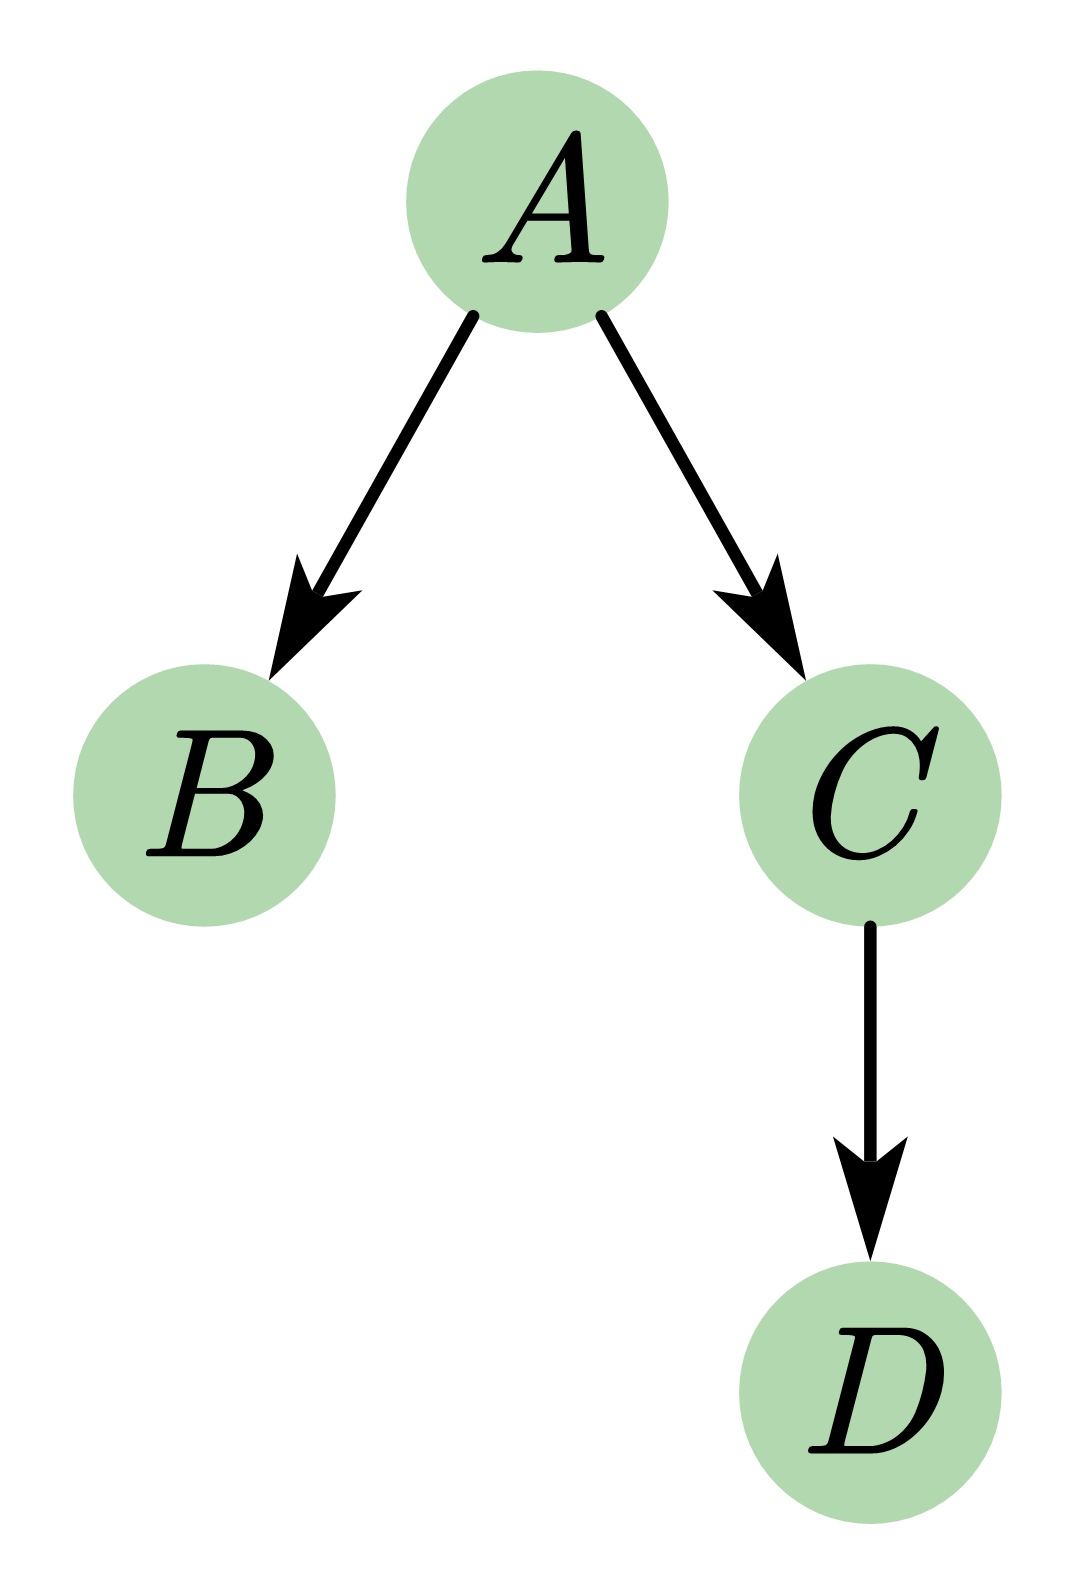
\includegraphics[width=3cm]{figure/BayesNet1.png}
\end{center}

表示概率分解:
\begin{empheq}{align*}
	P(A,B,C,D)&=P(A)P(B,C,D|A)\\
	&=P(A)P(B|A)P(C,D|A)\\
	&=P(A)P(B|A)P(D|C)P(C|A)\\
\end{empheq}

\subsubsection{等价类}
一个马尔科夫网的等价类是指:\circled{1}骨架相同;\circled{2}非正规结构(V结构)相同.骨架是指不考虑边的方向得到的边集.V结构形如:$X\rightarrow Z\leftarrow Y$,即双因.由于$Z$是由两个原因共同导致的,假如确定了$Z$,$X,Y$并不是独立,只有在某些情况下,才能共同诱导$Z$的特定值.

\subsubsection{do操作}
$\doop$也叫干预查询.图结构如下所示:
\begin{center}
	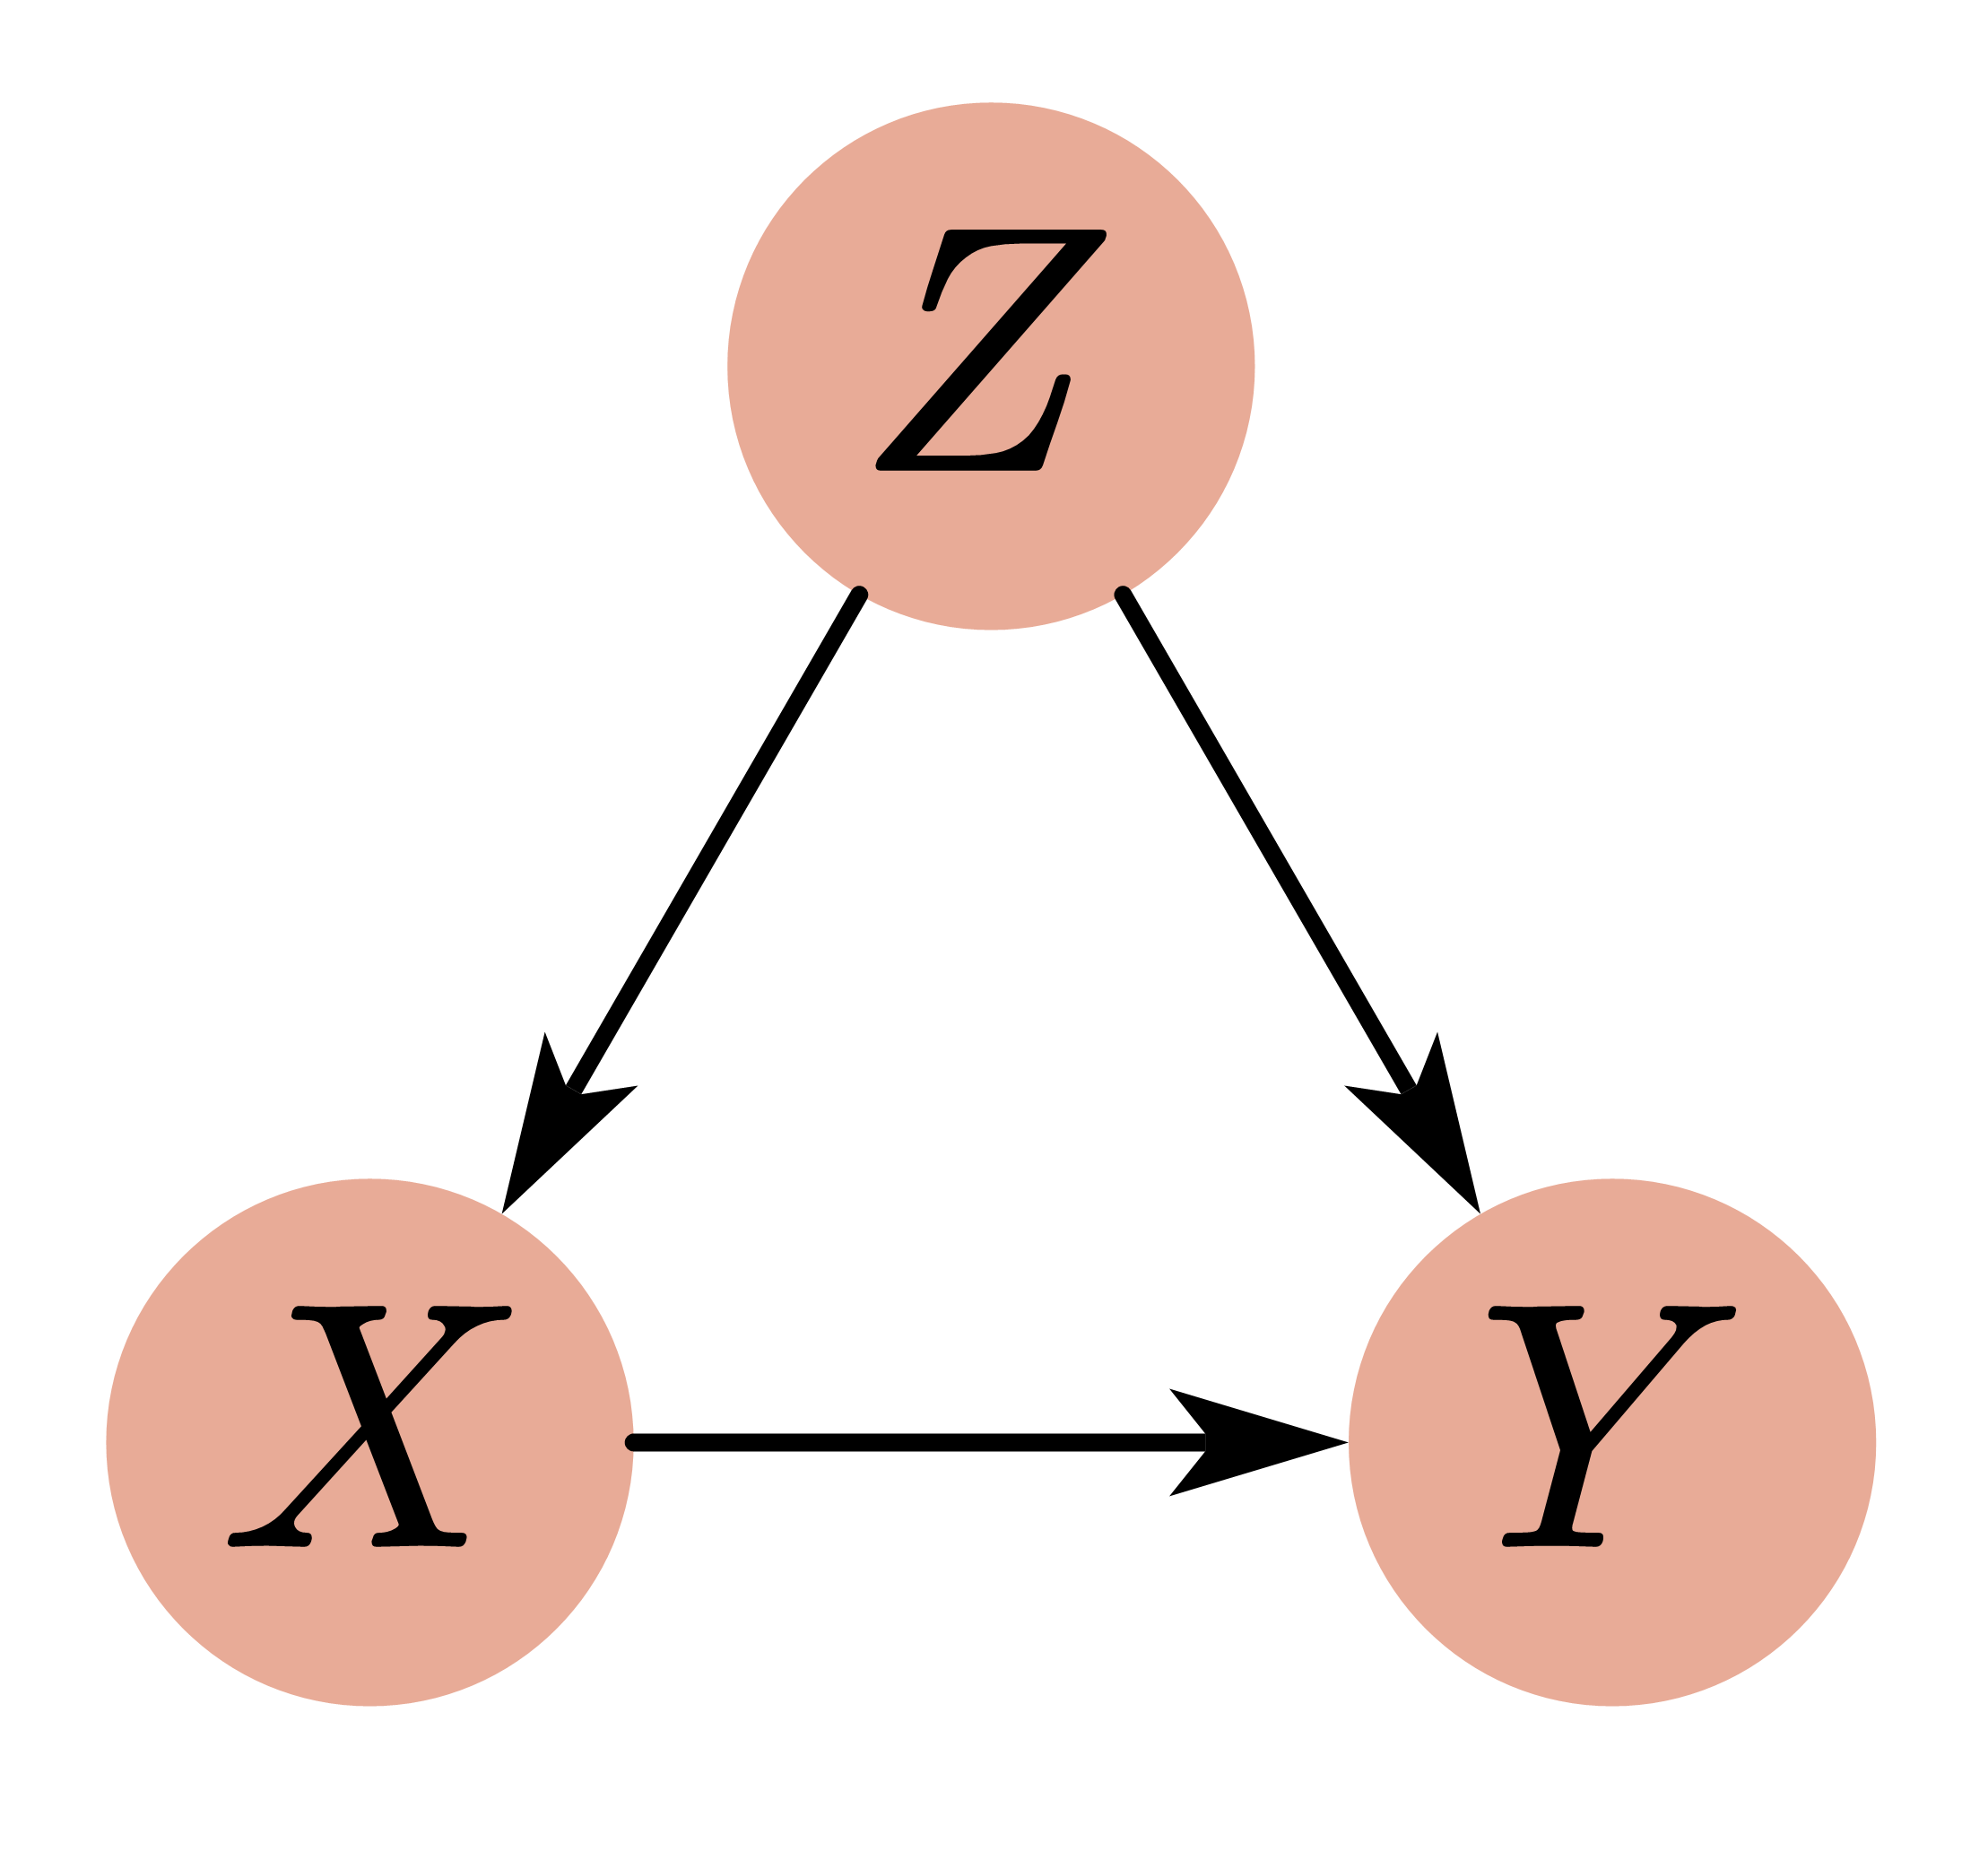
\includegraphics[width=3cm]{figure/Cofounder.png}
	\captionof{figure}{三变量网络}
	\label{fig:p5f1}
\end{center}

如果直接计算条件概率
\begin{empheq}{align*}
	\Prob(Y=y|X=x)&=\frac{\Prob(Y=y,X=x)}{\Prob(X=x)}\\
	&=\frac{\sum_z \Prob(Y=y,X=x|Z=z)\Prob(Z=z) }{\Prob(X=x)}\\
	&=\frac{\sum_z \Prob(Y=y|X=x,Z=z)\Prob(X=x|Z=z)P(Z=z) }{\Prob(X=x)}\\
	&=\frac{\sum_z \Prob(Y=y|X=x,Z=z)\Prob(X=x,Z=z) }{\Prob(X=x)}\\
	&=\sum_z \Prob(Y=y|X=x,Z=z)\Prob(Z=z|X=x)\label{condprob}
\end{empheq}

原本变量$X$由$Z$驱动,但使用$\doop X=x$操作后,$Z$就无法再影响$X$了,所以现在的图应当是
\begin{center}
	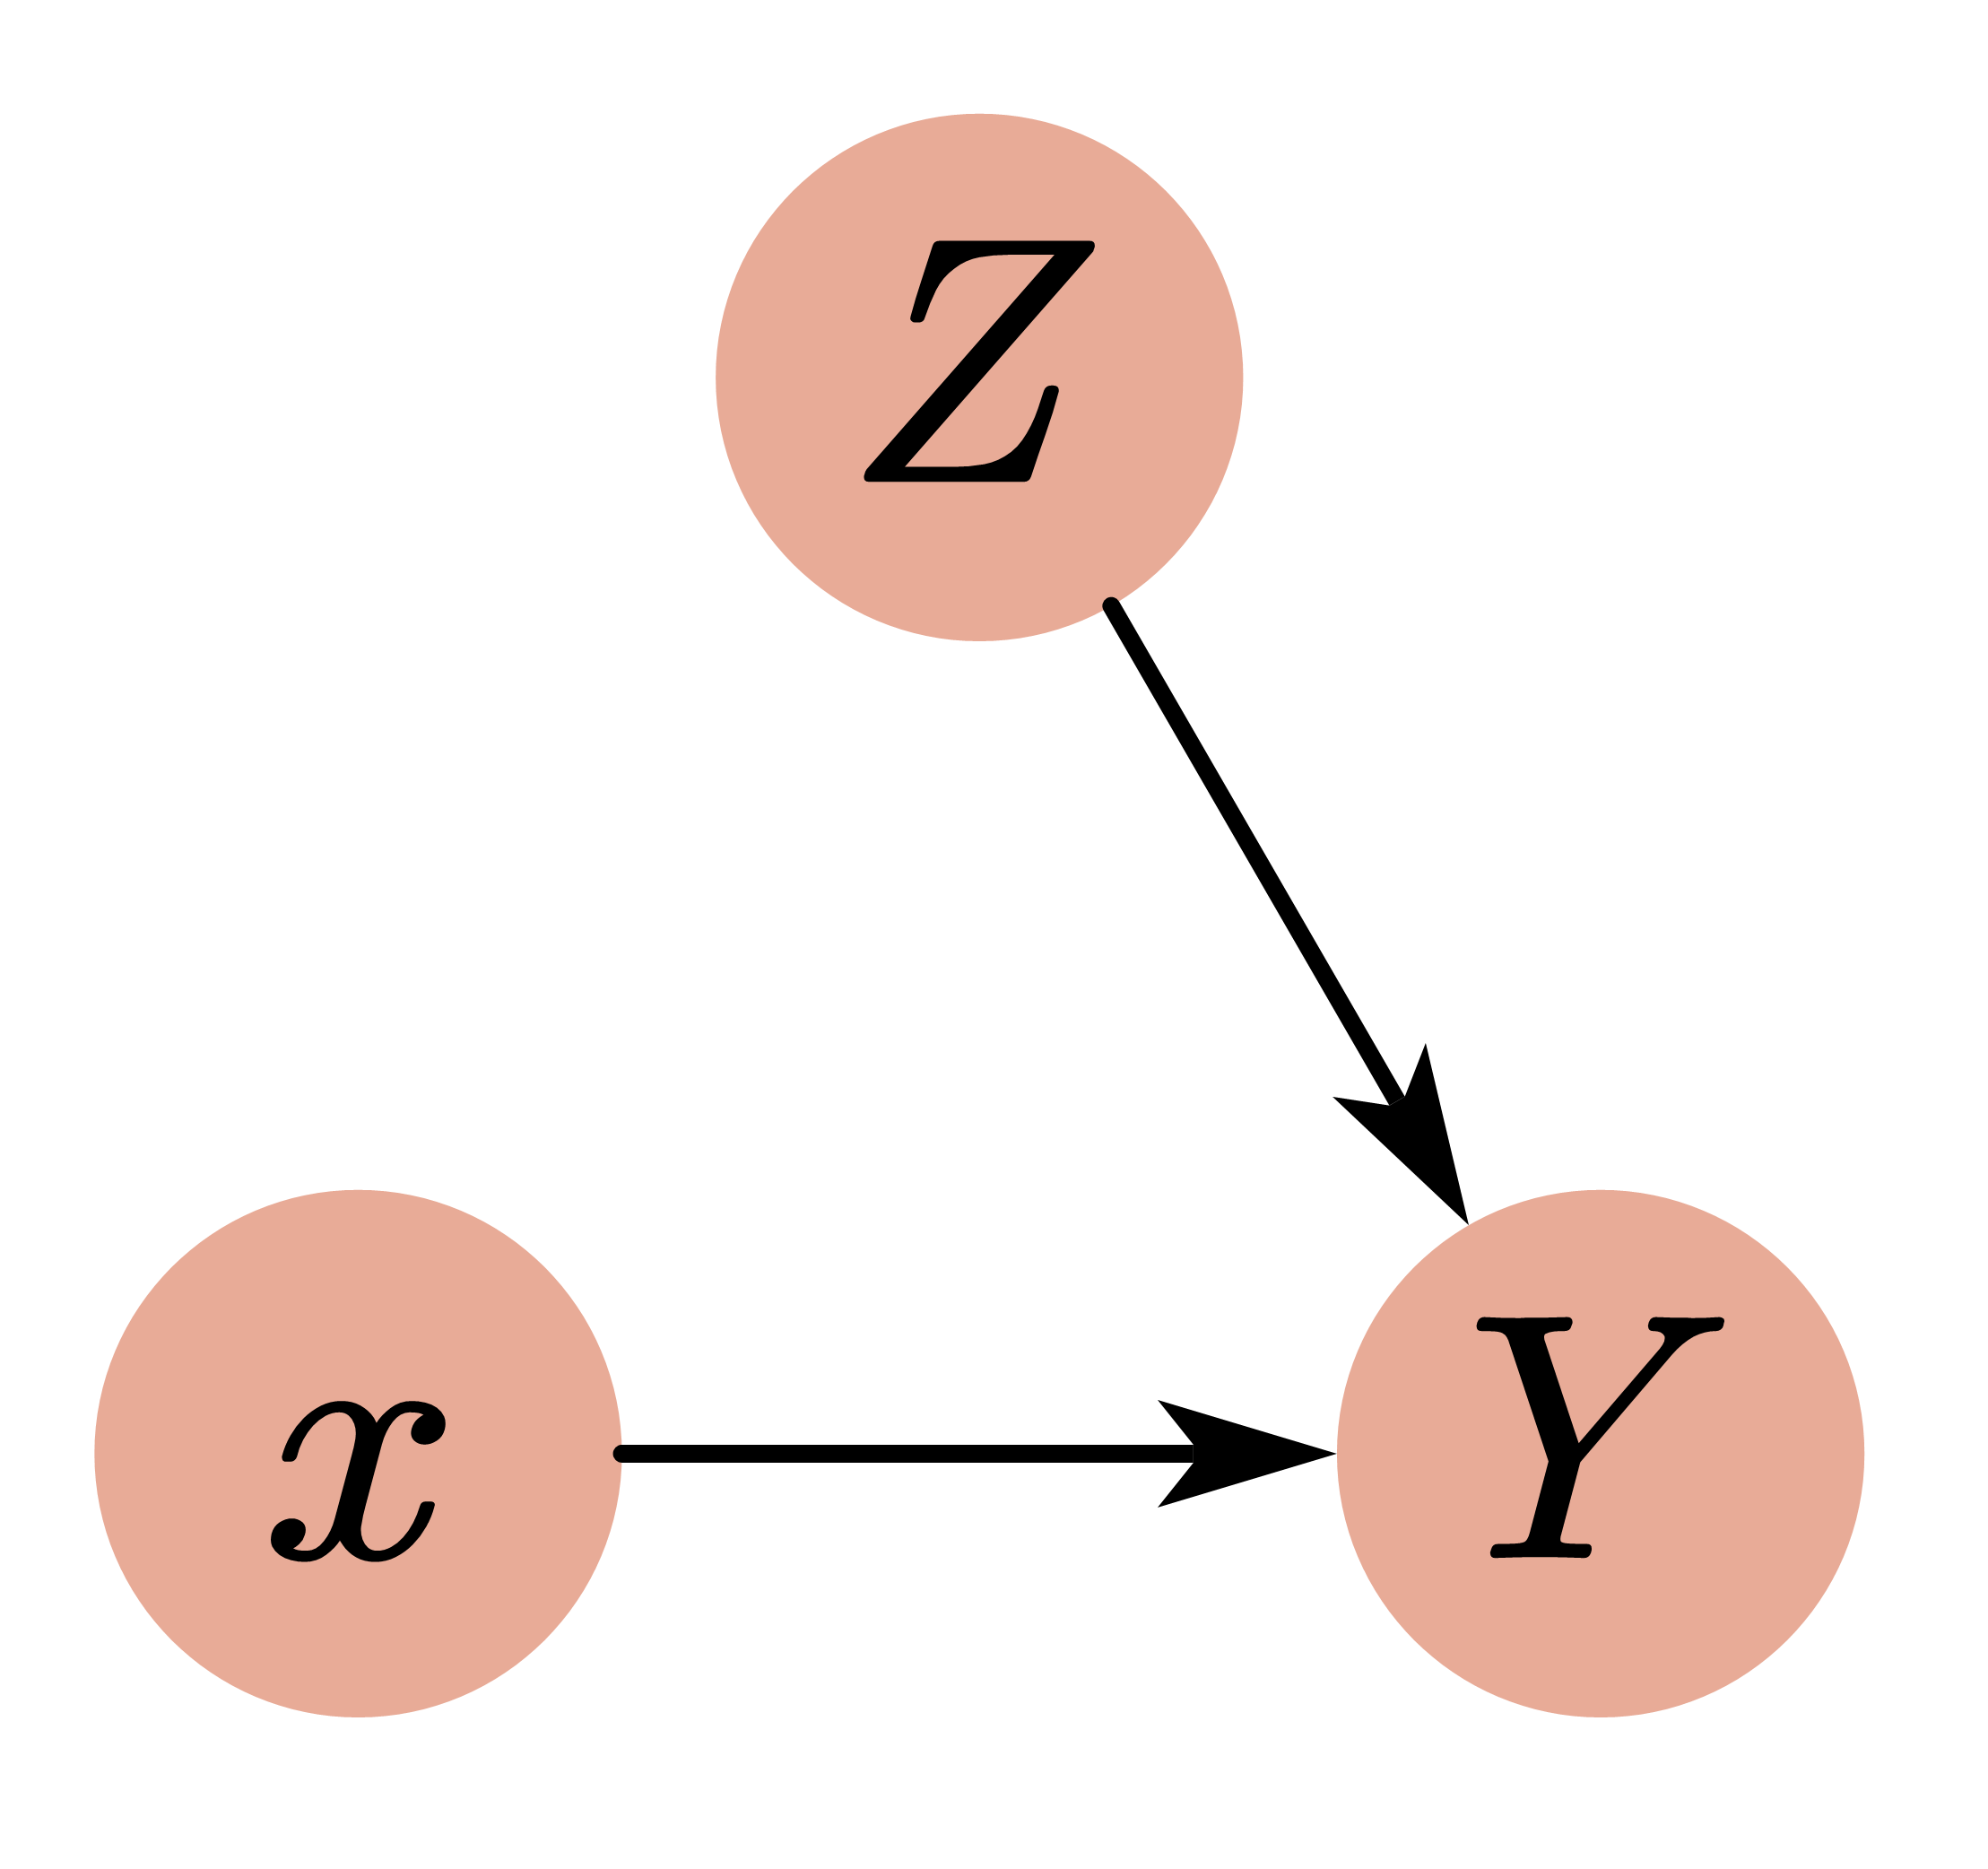
\includegraphics[width=3cm]{figure/bivar.png}
\end{center}
上图中$x$表示$X=x$,注意它现在已经不再是随机变量了,一下可以看出
\begin{empheq}{align}
	\Prob(Y=y|\doop X=x)&=\sum_z\Prob(Y=y|X=x,Z=z)\Prob(Z=z)\label{doprob}
\end{empheq}

之所以可以一步这样写,是因为$x$不是随机变量,而是类似于参数,假如暂时忽略它,那么就是
\begin{empheq}{align*}
	\Prob(Y=y)&=\sum_z\Prob(Y=y|Z=z)\Prob(Z=z)
\end{empheq}

现在把参数$x$加进去,就可以得到\eqref{doprob}.

以上可以看出,$\doop$操作的实质就是阻断因果关系.

另一方面,使用$\doop$后,$X$仍然可以理解为随机变量,但现在$\Prob(X=x)=1$,把这个条件加入\eqref{condprob}中,可以得到
\begin{empheq}{align*}
	\Prob(Y=y|X=x)
	&=\sum_z \Prob(Y=y|X=x,Z=z)\Prob(Z=z|X=x)\\
	\xRightarrow{P(X=x)=1}&\sum_z \Prob(Y=y|X=x,Z=z)\Prob(Z=z|1)\\
	&=\sum_z \Prob(Y=y|X=x,Z=z)\Prob(Z=z)\\
	\implies&\Prob(Y=y|\doop X=x)
\end{empheq}

这样我们从两个角度理解了$\doop$操作的实质.
\subsection{推理与计算}


\subsubsection{}

\chapter{神经网络与深度学习}

\section{数学基础与基本理解}
\subsection{深度与广度}
最基本的神经网络本质上就是一层套一层的连续变换

\begin{empheq}{align*}
\bm{y}&=\bm{f}_1(\bm{f}_2(\bm{f}_3\cdots(\bx)))\\
\bm{f}_i(\bx)&=\bm{\sigma}_i(W_i\bx+\mathbf{b}_i)
\end{empheq}

$\bm{\sigma}_i$就是激活函数,如果不加,那就是矩阵连乘.由于求导的链式法则,当导数小于1的时候,乘起来很快就变成0了,这是梯度消失;如果导数绝对值大于1,乘起来又可能变得很大,这是梯度爆炸.

激活函数一定要是非线性的,否则连续线性变换最终还是线性的.一般使用的激活函数是ReLU,它在大于0时是线性的,小于0时也是线性的.假如网络规模较小,比如就是传统的几层网络.那么当初始化后,假如恰好每一层的输出都大于0,那么就是线性的,此时梯度下降可能失效,导致最后训练出一个线性函数.此时必须引入更多的非线性.另一方面,只使用少数层可能使得所有输出大于0,但是假如提高深度,也可以增加非线性.

实际测试中发现,一个$1\rightarrow 5\rightarrow 10\rightarrow 1$的网络,如果全用ReLU激活函数,很容易习得一个线性函数,假如把其中一层改成ELU,那么就可以习得非线性.假如提高深度,中间中4层,那么也很容易习得非线性.这可能是说深度比广度更加重要一些.也说明网络效果与激活函数与初始化方式有关.


\paragraph*{为什么深度比广度更加重要}基本原因是用简单的事物来构造复杂的事物,一定要经过多次连续变换才行,即层次性.日常编程也是如此,需要对数据复合很多次才能得到目标结果.

从连续性的角度来理解,简单的事物,经过小的变换,是连续的,得到的新东西相比以前相差还不十分多,所以要经过很多变换才能得到目标.

在数学上,衡量一个函数的复杂性:极值的数量、不连续点的数量等等.

神经网络就是用简单的函数来逼近复杂的函数:加法、乘法、基本函数.


\paragraph*{连续变换} 从信息论的角度讲,做变换就可能造成信息损失,所以整个网络的表达能力取决于中间层的最小宽度和深度.

为什么残差网络有用,连续变换过程中丢失了信息,现在把原来的信息再传一遍,起到了一个增强的作用.

从表示论的角度中,中间层就是用一种新形式来表达原来的输入.这就与所谓的流形学习有关——现实中的高维数据通常可以用更小的维度来表达.

非光滑函数经过变换,通常还是非光滑的,这启示我们如果想逼近光滑函数,应该用光滑激活函数如$\tanh x$.如果想逼近非光滑的函数,如分类问题,应该用非光滑激活函数如$\ReLU,\HardTanh$.

连续线性变换,还是线性变换,包括卷积在内都属于线性变换.

\subsection{理解非线性}
非线性有不同的类型,比如对于CV来说,非线性可能是指Piecewise的非线性,就是分为很多段,但在局部仍然是接近线性的.在这种情形下,用ReLU就非常合适,因为它本身就适合描述if else判断.

有的非线性是指在整个区间上光滑,但是不同局部的增长速度不同.增长速度大致可以分为多项式或者指数级.可以设想,对于指数增长,用ReLU可能就不合适,因为复合线性乘法,本质上是多项式增长的,没法实现指数增长.

在这样的理念引导之下,我们可以设想,假如拟合超过多项式增长的函数,就引入一层指数函数.

非线性中尤其强调离散,注意离散是非线性,常用的Bool逻辑就属于离散函数.

\subsection{用神经网络表达各种函数}
\subsubsection{$\max$}
二维时:
$$\max (x,y)=\ReLU (x-y)+y$$

$n$维时,有几种思路.比如第一种:每次比较两个,选最大的,进行$n-1$次比较选出最大值,这样构造出来有$n-1$层.或者构造一棵树,一次比较$n/2$对,需要$n/2$层.

\subsubsection{两段直线}
\[
f(x)=\begin{cases}
	\frac{1}{3}x&,\ \text{if} x<=0 \\
	x&,\ \text{otherwise}
\end{cases}
\]

原点左边斜率为$\frac{1}{3}$,右边为$1$.这可以用$\ReLU$与$\sign$合成:
\begin{empheq}{align*}
f(x)&=\frac{1}{3}x+\frac{2}{3}\ReLU x\\
&=-\frac{1}{3}\sign (x) x+\frac{4}{3}\ReLU x
\end{empheq}


\subsection{作为核方法的深度学习}
有文章指出:使用梯度下降法学习的模型本质上近似于核方法\ref{deep_learning_as_ker}。所谓核方法就是简单地记忆数据,然后在遇到新样本时,通过查询、整合相似的记忆来输出结果。

本文中认为核心方法形如:
$$y=g\sbra{\sum_i a_i K(x,x_i)+b}$$
$g$为非线性函数,$a_i$为参数,在监督学习中通常就是$y_i$。$x_i$为已有样本,所以这是在说$x$的结果是其它样本的结果按相似度进行组合。

文章中提出了两种核
\begin{empheq}{align*}
K_{f,v}^g(x,x')&=\nabla_wf_w(x)\cdot \nabla_wf_w(x') \mtag{Tangent Kernel}\\
K_{f,c}^p(x,x')&=\int_{c(t)}K_{f,w}^g(x,x')\dif t \mtag{Path Kernel}
\end{empheq}


但文章也指出,一个SVM相当于单层的神经网络。而深度学习模型并不能简单地化简为核方法,因为它相比浅层网络可以表示指数级的复杂度,只是使用梯度下降法学习的模型相当于核方法。

\subsection{完备基函数组与参数效率、表达能力}\label{neural-network-basis-function}
神经网络是在用一些基本的Building block搭建整体,那么所选择的building block必定要具有某种“完备性”,才能具有足够的表达能力。一个简单的例子是用全连接层是很难表达$y=x_1x_2$的,全连接层的基本模型是
$$y=A_3\sigma(A_2\sigma(A_1\bx+\bm{b}_1)+\bm{b}_2)+\bm{b}_3$$
如果抛开激活函数不看,那么输出就是线性组合,并不存在输入之间的边乘项,猜想是不能准确地表达$x_1x_2$。

以下说明完全基函数组,首先是二元运算:
\begin{description}
\item[矩阵乘法] 内积$\cdot$也属于矩阵乘法。
\item[加法+]
\item[element-wise乘法$\otimes$]
\item[拼接Concatenate$\|$]
\end{description}
再配上激活函数或者一些一元运算:
\begin{description}
\item[$\min,\max$] $\ReLU$激活函数可以表达这两种。
\item[$\exp$]
\item[$\text{pow}$] 乘方。
\item[复制] 复制这个操作一般是隐含的,比如在卷积网络中,输入一个图片,可以用多个Features卷积产生输出,其实就包含了复制操作。
\item[缩放] 标量乘法。softmax可以由$\exp$与缩放复合而成。
\end{description}

二元运算虽然比较少,但是分左和右。神经网络的信息分参数与输入,那么每种运算至少有$(2+1)\times(2+1)=9$种可能,一下就非常多了。2和1是指参数与输入,1是指混合,不过只有参数与参数运算,意义不大,去掉这一种,至少也有8种。同时参数与输入还有顺序关系,比如残差层使用了之前的输出,可能的情况会更多。

观察大多数神经网络,都使用了以上结构,Transformer可能是最复杂的,基本把以上都包含了。

\subsection{拟合指数增长函数}
拟合指数增长函数并不是一件容易的事。首先一般的线性模型、多项式模型都无法做到,无论使用何种分布假设、使用马尔科夫链。神经网络中假如使用$\ReLU$激活函数,那么本质上是局部线性的,也不可能准确拟合指数增长函数。

有几种思路,要么改进模型,增加相应的基函数组,要么对数据进行变换,使之线性化。比如对数据取$\ln$变换。变换的思路可以应用于神经网络中,比如中间某一层,首先取$\ln(\ReLU(x)+1),\ln(\text{sigmoid}(x))$,经过线性组合后,再取$\exp$,如果直接使用$\exp$可能出现溢出。

金融领域中,有些股票的价格就是呈现指数增长状态的。

对于分类模型而言,随着深度的增加,树的分支也是呈现指数增长的,这种指数增长不能通过取对数来处理。使用传统的神经网络模型显然无法准确地处理,这也是研究双曲神经网络的一个重要原因,它适用于描述指数增长。

\subsection{初始化}
\subsubsection{Kamming}
\begin{equation}
W=U/\sqrt{out/2}
\end{equation}
以上中$out$表示输出的大小。
\section{各种神经网络层}
\subsection{Convolution}
Convolution就是局部元素的线性组合,相当于把全连接层拆分.假如对一个序列自身进行Convolution,就是自回归,两个序列进行Convolution,就是线性回归.以下说明一些基本概念.

\paragraph*{channel}Chanel本来是图像中的概念,比如一般的彩色图片有三个Channel,每个Channel是一个矩阵.对于1D的情形,输入向量$n\times1$,可以视为1个Channel.

\paragraph*{padding}在1D的情形,假如序列长度为$n$,取长为$k$的核,那么输出为$n-k+1$,长度缩短了,需要在输入的两边补充0元素来使输出进行扩张.

\paragraph*{stride}每次核移动多少距离,一般是取1.移动的距离越短,则输出越少.

\paragraph*{dialation}间距.一般是取连续的元素与核进行合成,现在用不连续的元素来合成,就是dialation.

\paragraph*{group}默认是1,要求in\_channels和out\_channels是它的倍数.核的数量=in\_channels/groups*out\_channels.见下图.使用分组可以直到截断关联的作用.取分组为1的时候,输出的每个Channel是由所有输入的channel复合而成.如果取分组为in\_channel,那么就叫depth-wise convolution,每个in\_channel展开成多个out\_channel.

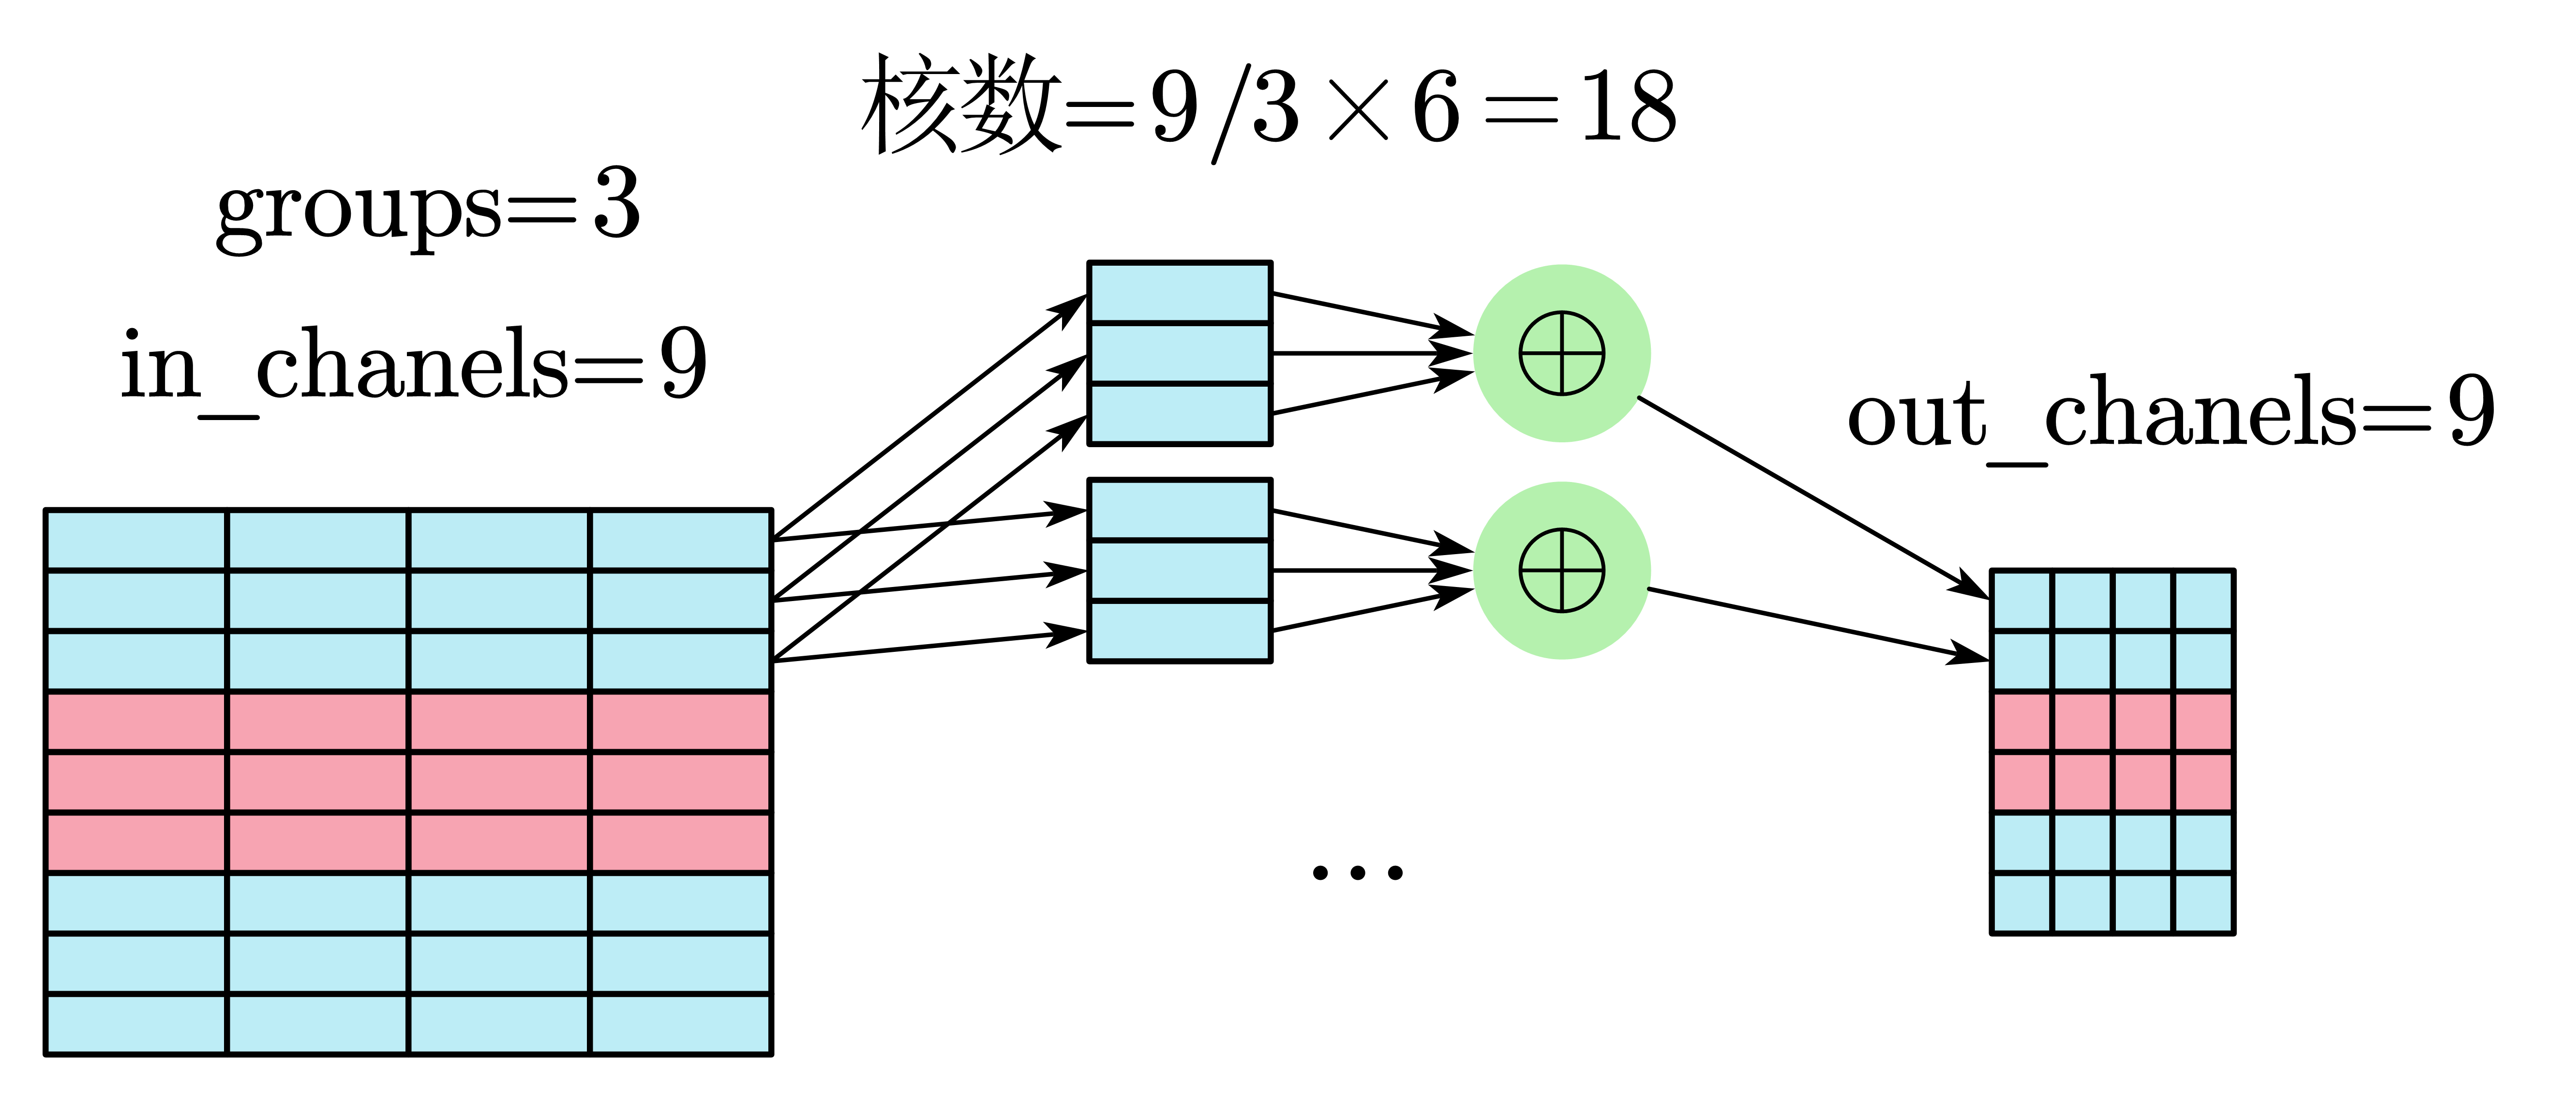
\includegraphics[width=\textwidth]{figure/Convolution-Groups.png}

注意图中,左边每次滑动移动距离为窗长,实践中一般是移动1.显然,Convolution捕捉的是局部相关性,因为它把相邻近的元素进行组合.

\subsection{LSTM层}
\subsubsection{数学表达式}

\begin{empheq}[left=\empheqlbrace]{align*}
\widetilde{\bm{c}}_t&=\tanh (W_c\bx_t+U_c\bm{h}_{t-1}+\bm{b}_c)\\
\bm{i}_t&=\sigma(W_i\bx_i+U_i\bm{h}_{t-1}+\bm{b}_i)\\
\bm{f}_t&=\sigma(W_f\bx_t+U_f\bm{h}_{t-1}+\bm{b}_f)\\
\bm{o}_t&=\sigma(W_o\bx_t+U_o\bm{h}_{t-1}+\bm{b}_o)\\
\bm{c}_t&=\bm{f}_t\odot\bm{c}_{t-1}+\bm{i}_t\odot\widetilde{\bm{c}}_t\\
\bm{h}_t&=\bm{o}_t\odot\tanh(\bm{c}_t)
\end{empheq}

\subsubsection{示意图}
一个LSTM Cell的结构如下图所示,图中的$N$表示输入(Batch Size为1,为向量,对应于Features或者Channel个数)的长度,$M$是Hidden size。

\begin{center}
\includegraphics[width=12cm]{figure/LSTM Cell.png}
\end{center}

可以从图中看出,参数的个数是$\underbrace{(M+N)\times N \times 4}_{\text{四个门的矩阵乘法}}+\underbrace{(M+N)\times 4}_{\text{四个门的偏移}}$。

一个LSTM层由多个LSTM Cell堆叠起来。整个层的输入通常是$(N,L,C)$,每次取1列送往网络进行计算,则每次的输入是$(N,C)$,最终的输出是$(N,C_H)$。如下图所示:

\begin{center}
	
\includegraphics[width=12cm]{figure/LSTM Sample.png}
\end{center}

\subsection{GRU层}
\subsubsection{数学表达式}
\begin{empheq}[left=\empheqlbrace]{align*}
\bm{h}_t&=\bm{z}_t\odot\bm{h}_{t-1}+(1-z_t)\odot \widetilde{\bm{h}}_t\\
\bm{z}_t&=\sigma(W_z\bx_t+U_z\bm{h}_{t-1}+\bm{b}_z)\\
\widetilde{\bm{h}}_t&=\tanh (W_h\bx_t+U_h(\bm{r}_t\odot\bm{h}_{t-1})+\bm{b}_h)\\
\bm{r}_t&=\sigma(W_r\bx_t+U_r\bm{h}_{t-1}+\bm{b}_r)
\end{empheq}
\subsubsection{示意图}

\begin{center}
\includegraphics[width=12cm]{figure/GRU cell.png}
\end{center}

\subsection{Residual层}
\subsubsection{数学表达式}
\begin{empheq}{align*}
\by&=\mathcal{F}(\bx)+\bx
\end{empheq}

\subsubsection{示意图}
\begin{center}
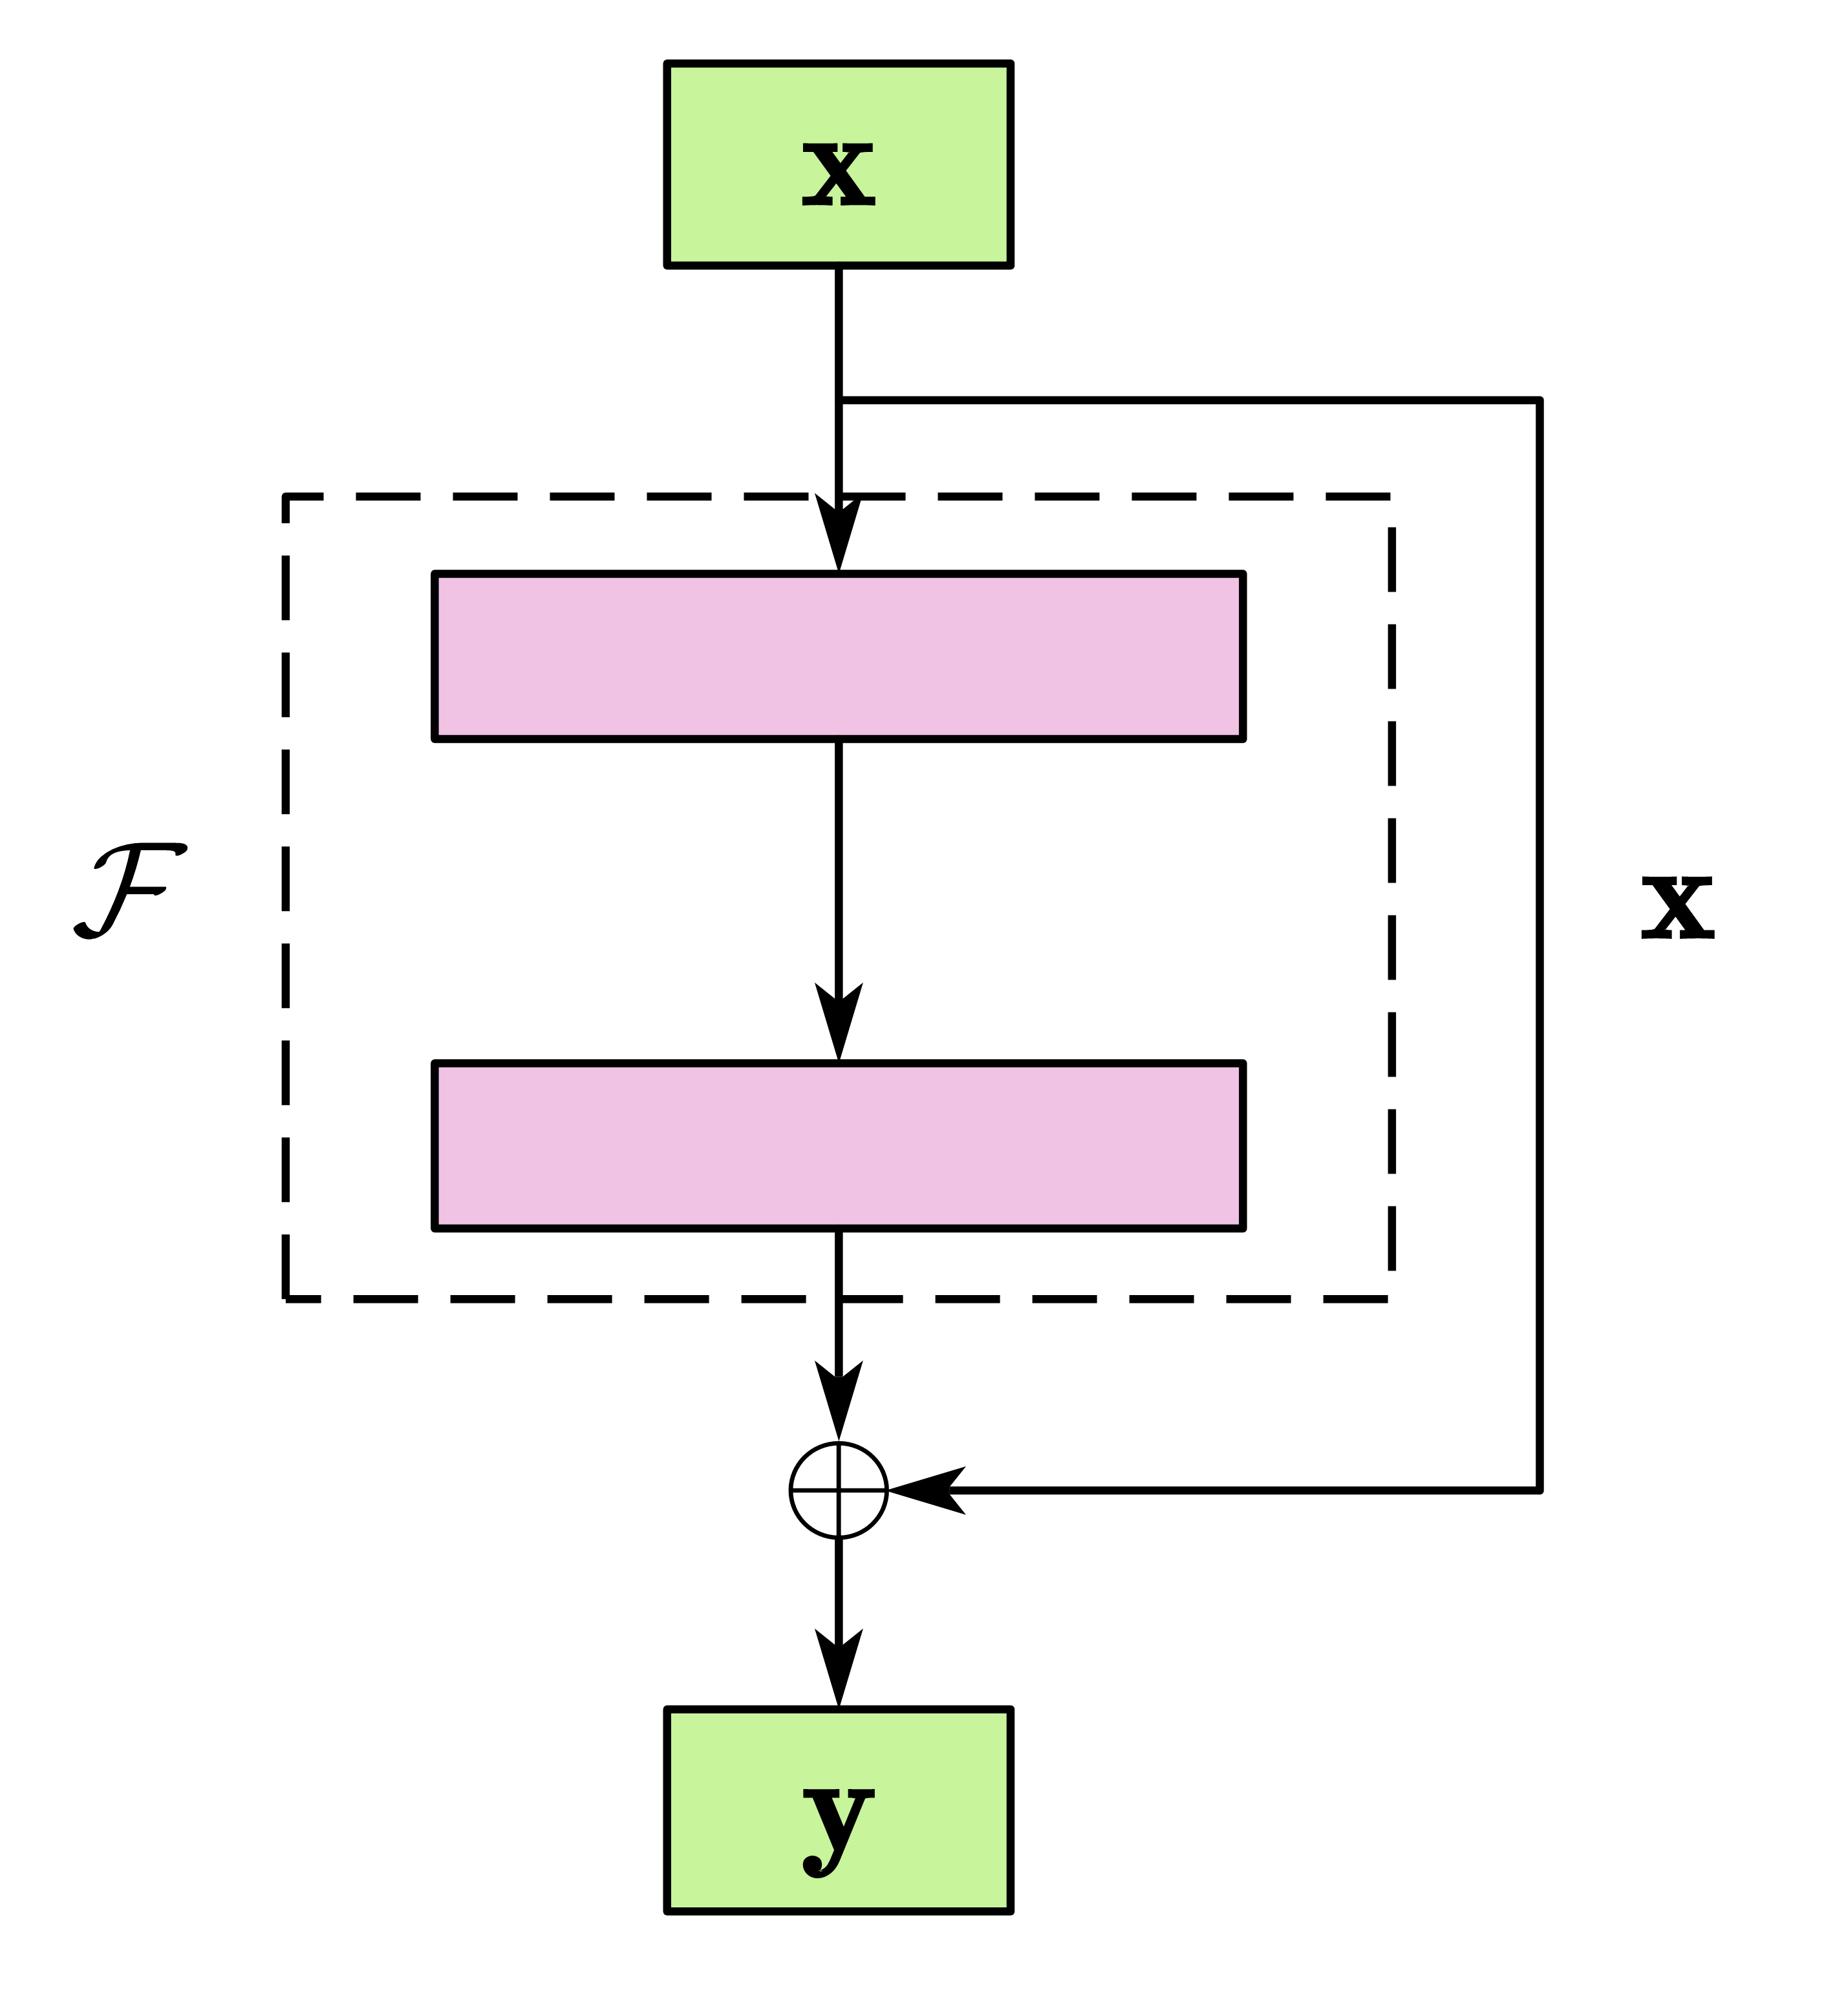
\includegraphics[width=6cm]{figure/Residual-block.png}
\end{center}

从图中可以看出,所谓残差是指
$$\mathcal{F}(\bx)=\by-\bx$$

此外,直接将输出传送到输出,也叫identity map by shortcuts,所谓identity就是指$\bx$.

\section{各种损失函数}


\section{各种激活函数}
注意$\sign$也可以用作激活函数.
\subsection{ReLU族}
特征是在输入小于0时输出接近0,而大于0时保持。

\subsubsection{ReLU}
函数形式:
\[
ReLU(x)=\begin{cases}
	0&,\ \text{if} x<=0 \\
	x&,\ \text{otherwise}
\end{cases}
\]

同时$\ReLU$也可以用$\sign$表达:
$$\ReLU(x)=\frac{1}{2}(\sign(x)+1)*x$$

\pgfplotsset{
	myplot/.style={
		width=8cm, height=4cm,
		xlabel=$x$, ylabel=$ReLU(x)$,
		samples=50,
		xlabel style={at={(1,0)}, anchor=west},
		ylabel style={rotate=-90, at={(0,1)}, anchor=south west},
		legend style={draw=none, fill=none},
		xmin=-3, xmax=3
	}
}
\begin{center}
	\begin{tikzpicture}[>=stealth,
		every node/.style={rounded corners},
		declare function={
			ReLU(\x)=((\x>0)*\x);
		}]
		
		\begin{axis}[myplot]
			\addplot[smooth, thick, domain=-3:3] {ReLU(x)};
		\end{axis}
	\end{tikzpicture}
\end{center}
\subsubsection{LeakyReLU}
ReLU加强版,负数不归0,而是用一条小斜率的直接取代.
\[
LeakyReLU(x)=\begin{cases}
	slope\times x&,\ \text{if} x<=0 \\
	x&,\ \text{otherwise}
\end{cases}
\]

$slope$在Pytorch中默认为0.01.
\subsubsection{PReLU}
LeakyReLU加强版,允许对输入为负数时的斜率进行学习:
\[
PReLU(x)=\begin{cases}
	ax&,\ \text{if} x<=0 \\
	x&,\ \text{otherwise}
\end{cases}
\]

$a$为一可学习的参数.按Pytorch官方的说法,使用这个激活函数时,不要用权重衰减.

\subsubsection{RReLU}
类似于PRELU,允许对输入为负数时的斜率进行学习:
\[
RReLU(x)=\begin{cases}
	ax&,\ \text{if} x<=0 \\
	x&,\ \text{otherwise}
\end{cases}
\]

$a$为随机采样的斜率.函数形式与RReLU完全一样。

\subsubsection{GeLU}

在Transformer中经常使用。

\[
\text{GeLU}(x)=x\Phi(x)
\]

\pgfplotsset{
	myplot/.style={
		width=8cm, height=4cm,
		xlabel=$x$, ylabel=$\text{GeLU}(x)$,
		samples=50,
		xlabel style={at={(1,0)}, anchor=west},
		ylabel style={rotate=-90, at={(0,1)}, anchor=south west},
		legend style={draw=none, fill=none},
		xmin=-3, xmax=3
	}
}
\begin{center}
	\begin{tikzpicture}[>=stealth,
		every node/.style={rounded corners},
		declare function={
			GeLU(\x)=x/(1 + exp(-0.07056*pow(\x,3) - 1.5976*\x));
		}]
		
		\begin{axis}[myplot]
			\addplot[smooth, thick, domain=-3:3] {GeLU(x)};
		\end{axis}
	\end{tikzpicture}
\end{center}

\subsection{tanh族}
特征是输出有界。

\subsubsection{tanh}
\pgfplotsset{
	myplot/.style={
		width=8cm, height=4cm,
		xlabel=$x$, ylabel=$tanh(x)$,
		samples=50,
		xlabel style={at={(1,0)}, anchor=west},
		ylabel style={rotate=-90, at={(0,1)}, anchor=south west},
		legend style={draw=none, fill=none},
		xmin=-3, xmax=3
	}
}
\begin{center}
	\begin{tikzpicture}[>=stealth,
		every node/.style={rounded corners},
		declare function={
			tanhf(\x)=tanh(x);
		}]
		
		\begin{axis}[myplot]
			\addplot[smooth, thick, domain=-3:3] {tanhf(x)};
		\end{axis}
	\end{tikzpicture}
\end{center}

\subsubsection{HardTanh}
函数形式:
\[
ReLU(x)=\begin{cases}
	-1&,\text{ if } x\leq-1 \\
	x&,\text{ if } -1\leq x\leq 1 \\
	1&,\text{otherwise}
\end{cases}
\]

\pgfplotsset{
	myplot/.style={
		width=8cm, height=4cm,
		xlabel=$x$, ylabel=$HardTanh(x)$,
		samples=50,
		xlabel style={at={(1,0)}, anchor=west},
		ylabel style={rotate=-90, at={(0,1)}, anchor=south west},
		legend style={draw=none, fill=none},
		xmin=-3, xmax=3
	}
}
\begin{center}
	\begin{tikzpicture}[>=stealth,
		every node/.style={rounded corners},
		declare function={
			HardTanh(\x)=((\x>1)+(\x<-1)*(-1)+and(\x<1,\x>-1)*x);
		}]
		
		\begin{axis}[myplot]
			\addplot[smooth, thick, domain=-3:3] {HardTanh(x)};
		\end{axis}
	\end{tikzpicture}
\end{center}

\subsection{Huber族}
\subsubsection{Huber Loss}
$$L_\delta(x)=\begin{cases}
\frac{1}{2}x^2&\text{ if } |x|\leq \delta \\
\delta x-\fh\delta^2 & \text{ otherwise }
\end{cases}$$
可以自然地拓展到进行函数逼近:
$$L_\delta(y,f(x))=\begin{cases}
	\frac{1}{2}(y-f(x))^2&\text{ if } |y-f(x)|\leq \delta \\
	\delta|y-f(x)|-\fh\delta^2 & \text{ otherwise }
\end{cases}$$

在靠近0的小区域内,它是二次的,在外面,它是线性的。而且本函数是光滑的。

\subsection{归一化类}
\subsubsection{softmax类}
\paragraph*{原始softmax}可以用来限定和为1,且值为正数,因此用来表示概率。
$$\softmax(x_i)=\frac{\exp(x_i)}{\sum \exp(x_i)}$$

\paragraph*{log-softmax}
$$\text{log-softmax}(\bx)=\ln(\softmax(\bx))\approx \bx-\max(\bx),x_i\in(-\infty, 0]$$
$\sum \exp(x_i)$会被,较大的数所主导,所以$\ln\left(\sum x_i\right)\approx \max (\bx)$。
\paragraph*{其它变体}
\begin{enumerate}
	\item 限定和为1,且有正负:$$n\softmax(\bx)-\frac{n-1}{n},x_i\in\left(-\frac{n-1}{n},n-1+\inv{n}\right)$$可以用来表示可以做空的投资权重。另一种方式是直接用绝对值归一化:
$$\frac{\bx}{\sum |x_i|},x_i'\in[-1,1]$$
但这种表示方法是仅仅绝对值之和为1,和是不确定的,而且因为有除法,不容易训练。
\item 在上一种方法上进行扩展:
$$a\softmax(\bx)-\frac{a-1}{n}$$
值域为
$$	x_i\in\begin{cases}
\left(-\frac{a-1}{n},\frac{n-1}{n}a+\inv{n}\right),&\text{if } a>0\\
	\left(\frac{n-1}{n}a+\inv{n}, -\frac{a-1}{n}\right) &\text{if } a<0
\end{cases}$$
\begin{note}
	\begin{enumerate}
		\item 如果希望限定最大值,比如对于3个数,取
		$$a-1+\frac{1}{n}\leq 1\implies a\leq \frac{3}{2}$$
		假如令$a=\frac{3}{2}$,则$x_i'\geq -\inv{2n}$,非常接近0了,不算太理想。
		
		要使下界小于0,必然有$a\geq 1$,上界$\geq \inv{n}$。
		\item 区间的长度为$\lvert\frac{n+1}{n}a-1\rvert$。
		\item 如果希望区间对称,则$\frac{a-1}{n}=\frac{n-1}{n}a+\inv{n}$,此时$a=\frac{2}{2-n}<0\rightarrow 0,x_i'\in\left(-\inv{n-2},\inv{n-2}\right)$,对于3个数,取$a=-2$,则区间为$(-1,1)$,这比较理想。如果$n=10,a=-\inv{4},x_i'\in\left(-\inv{8}, \inv{8}\right)$,不太理想。这个变换界卡得太死了。
		\item 由于$\softmax$值域是大于0的,线性变换要使区间对称,必然需要左偏,则$a<0$。
	\end{enumerate}

\end{note}
\end{enumerate}
\subsubsection{有界投影法}
考虑这样一种操作,首先把输出变换成有界区间$[a,b]$,再投影到平面$\sum x_i=1$平面上,由于输入有界,则投影后也有界,而且这个界易于自己控制。这样得到的结果是:
\begin{equation}\label{constrained-projection-normalize}
x_i'=\frac{1-\sum x_i}{n}+x_i
\end{equation}
这个变换的矩阵表示为:
$$\bx'=\left(I-\inv{n}\bm{1}_{n\times n}\right)\bx+\inv{n}\bm{1}_{n\times 1}$$
这个矩阵是不可逆的。

注意到\ref{constrained-projection-normalize}是一个线性变换,它会把极点变换成极点,但$[-a,\bm{0}]$显然不是极点,所以不应该代入这个。应该取$[-b,\bm{a}]$和$[a,-\bm{b}]$,输出界为
$$\left[\inv{n}-\frac{-b+(n-1)a}{n}-b,\inv{n}-\frac{a-(n-1)b}{n}+a\right]$$
仍然不对称。而且注意到,上下界之和为$\frac{2}{n}$,因此必然不可能对称,不过在$n$比较大时,差别就很小了。

如果约束上界为$u$,为方便计算,取$a=b$,那么解得
$$a=b=\frac{nu-1}{2n-2}$$
在$u=1$时,$a=b=\inv{2}$,此与维度无关,下界为$\frac{2}{n}-1$。
\section{各种网络结构}
\subsection{GAN}
\subsubsection{原始GAN}
原始GAN模型\cite{goodfellow2014generative}由两个部分组成:生成器、判别器。前者的任务是从先验(通常取均匀分布或者高斯分布)中生成服从目标分布的数据,而判别器的任务是判断生成的数据是否符合目标分布。从结果上看,生成器起到了将先验分布变换为目标分布的作用。图示如下:

\begin{center}
	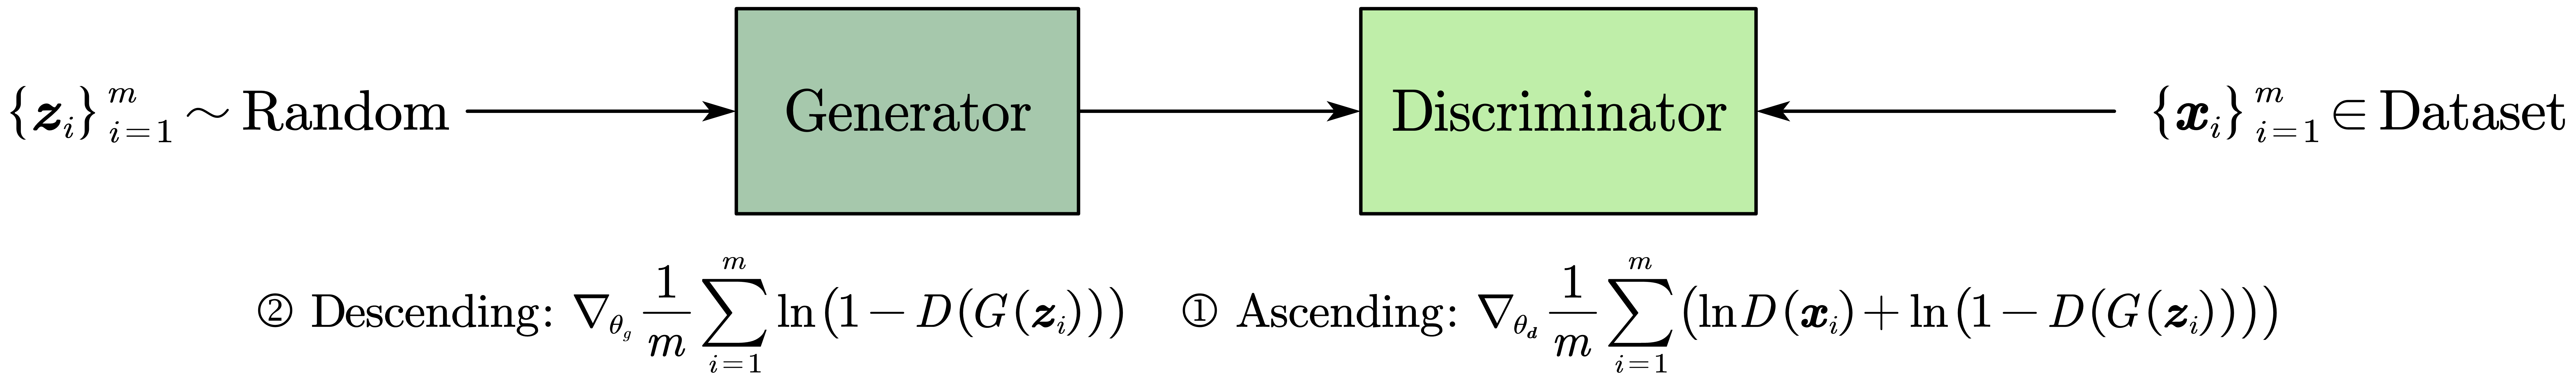
\includegraphics[width=15cm]{GAN.png}
\end{center}

如图所示,模型更新过程分为两个步骤,首先更新判别器,使用的是梯度上升,极大化目标函数。理想情况下$D(x)\rightarrow 1,D(G(z))\rightarrow 0$。需要注意的是,判别器是一个二分类器,输入只有1个,判断这个样本是不是目标分布,并非输入为2个。


再更新生成器。更新生成器时,进行梯度下降使用的样本是新生成的样本,并非第一步里面生成的样本。

从更新过程中可以看出,判别器不是越强越好。假如判别器的能力是无限的,那么$D(G(z))=0$,第二步更新生成器的过程就没有用了。

实际来看,GAN是比较难训练的。推荐以下策略:
\begin{enumerate}
\item 学习率不能太低,大概可以设成1e-5这样。可以使用衰减策略。
\item 分类器的学习率可以设成比生成器学习率低,一般可以取后者的1/10。
\item 
\end{enumerate}

\subsubsection{应用GAN}
\paragraph*{时间序列预测}下图来自\cite{ZHANG2019400}。模型结构如图所示:
\begin{center}
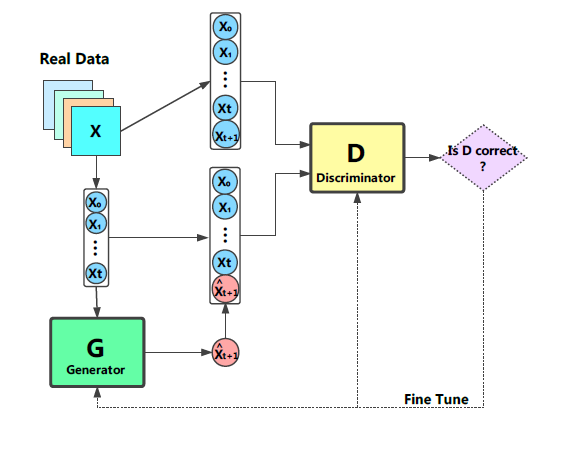
\includegraphics[width=10cm]{figure/gan-in-stock-pred.png}
\end{center}

核心在于生成器给出前向预测。

\subsection{Transformer}

\subsubsection{网络参数结构}
pytorch中,一个
\begin{verbatim}
	torch.nn.Transformer(d_model=10, nhead=5,dim_feedforward=200)
\end{verbatim}
的参数数量为59080。默认构造函数的参数是num\_encoder\_layers =num\_decoder\_layers=6。网络参数结构如下:
\begin{empheq}{align*}
\underbrace{\begin{bmatrix}
	300 & 30 & 100 & 10 \end{bmatrix}}_{\text{Multi-head Attention}}\underbrace{\begin{bmatrix} 2000 & 200 & 2000 & 10\end{bmatrix}}_{\text{FF}}\begin{bmatrix}
	10\times 4
\end{bmatrix}
\times 6 &=28140\\
\begin{bmatrix}
10
\end{bmatrix} &=5\\
\begin{bmatrix}
10&10 &	300 & 30 & 100 & 10 &300 & 30 & 100 & 10\end{bmatrix}
\underbrace{\begin{bmatrix} 2000 & 200 & 2000 & 10\end{bmatrix}}_{\text{FF}}
\begin{bmatrix}
10\times 4
\end{bmatrix}\times 6&=14850\\
\begin{bmatrix}
10\times 4
\end{bmatrix}&=15\\
&=28940
\end{empheq}

\subsubsection{示意图}
Transformer可以调用现成的库作为层调用,但其实内部比较复杂,更接近架构的概念,而非普通的层。表示为
$$(L_1,N,C)\times (L_2, N, C)\rightarrow (L_2, N, C)$$

此处引用一张广为流传的图:
\begin{center}
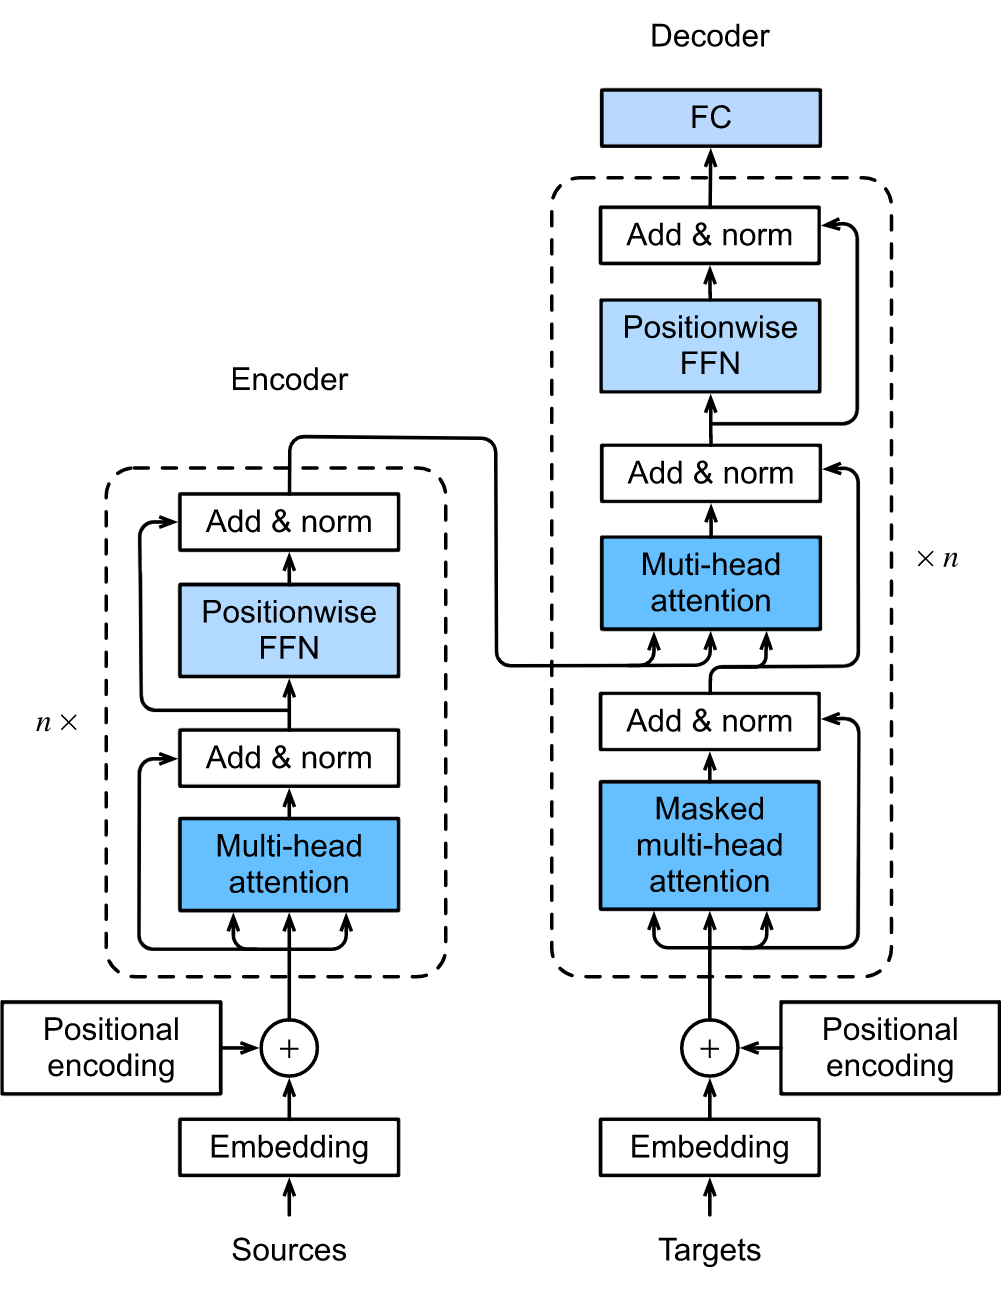
\includegraphics[width=10cm]{figure/TransformerArch.png}
\end{center}
Encoder与Decoder的结构是相似的,只是多了一层Attention。需要强调的是,Encoder的最终输出要送往Decoder的每一层。

下图对照之前的参数结构,给出Encoder一层的结构,没有画出BatchNorm层:
\begin{center}
\includegraphics[width=12cm]{figure/Transformer.png}
\end{center}

大致上是分两部分,首先是Attention层,再加上Linear层。Attention会把输入复制一下送到不同的head和$Q,K,V$。本质上是矩阵乘法、拼接。

其中FF层是
\begin{empheq}{equation*}
\by=W_2\max(0, W_1\bx+\bm{b}_1)+\bm{b}_2
\end{empheq}
现在对照之前的列表,即可看出,$W_1$是$d_{\text{model}}\times d_{\text{ff}}$,对应之前的$10\times 200=2000$,再加上偏移即可。$W_2$是$d_{\text{ff}}\times d_{\text{model}}$,也是2000。

从图中也可以看出,输入和输出的$C$必定等于模型的$d_{\text{model}}$,并且$d_{\text{model}}$必定整除\texttt{nhead}。

对于时间序列模型,输入通常有多个维度,但输出是1,即预测。此时一种直观的做法就是把输出进行复制,但不清楚这样是否合理。但这样一来,$Q,K,V$使用的参数就非常少,比如$C=5$,\texttt{nhead=1},则$Q$对应参数为$5\times 5=25$。或者还可以手动复制,比如5复制4份,得到$C=20$,增加参数数量。

此外,时间序列时用自变量预测因变量,可以把自变量的旧值作为Encoder输入,因变量的新值作为Decoder输入,然后下一时期的值作为输出。
\subsubsection{对比LSTM}
与LSTM相比,Transformer最大的差异就是没有维护内部状态,LSTM中是用$\bm{h,c}$来维护内部状态的。
\section{实践经验}
\subsection{最佳实践}
\begin{enumerate}
\item 使用残差连接。残差网络的性能比一般的网络稍好。但在训练过程中损失函数可能出现阶段式下降的情况,比如在某一阶段几次迭代过程中改变很小,之后才继续下降。尚不明确原因。

在回归中使用残差连接的一种方式就是LSTM+MLP+残差连接。在一次GAN-LSTM实践中,观察到在生成器中使用比LSTM+MLP的效果更好,如果只使LSTM+MLP,那么在MSE在降到最低点几百以后很快会上升,但残差连接不易出现这种情况,稳定性好。

不过残差网络在参数量相似的情况下,运行似乎有点慢。

\item 使用\texttt{gelu, leaky\_relu}一类的损失函数。
\item 使用$3\times3$的卷积核。卷积核不能太大.小的卷积核精度更高,大的卷积核容易丢失信息,一次实验中,使用10层卷积网络,核大小为5,一直只有0.5\%正确率,但降低为$3\times 3$后准确率立即提高了很多.
\item 多网络训练的同步问题.包括GAN之类的网络是由多个网络构成的,需要注意训练时的同步。主要是学习率需要好好设置,一般来说,更加关心的应该学习率设得高一些,比如GAN中的生成器,它的学习率可以设成判别器的10倍,此时相当于把生成器作为主要目标,而判别器作为辅助。GAN中判别器不能太强,也与网络的原理有关,如果判别器太强,则梯度很接近0,没法更新生成器。
\end{enumerate}


\subsection{不能随意使用卷积与ReLU}
在CV中,卷积通常可以起到边缘检测的作用,这要求数据在某个边界发生大的变动.同时ReLU会让很多数据归0,因此假如原本的数据变动不大(比如金融数据),而且有一定随机性,那么套上卷积与ReLU后,很容易使得结果归0.有人据此也认为ReLU函数发挥作用主要是因为正则化.假如此时加上一层全连接,那么起作用的实际上是bias,其它都归0了.

当然,归0也与参数的初始化方式有关,比如Pytorch中默认是均匀分布.大约有一半是负数,可能就比较容易全0.

为了防止归0,可以使用负数部分不归零的函数如PReLU、RReLU.


\subsection{BatchNorm}
使用BatchNorm可以降低损失函数的值,否则层层放大,可能导致损失函数异常大.有的网络中对每一层卷积都用了BatchNorm,可能过于频繁了,两层或更多加一个BatchNorm可能比较好.但BatchNorm本身对最终结果影响不大,只是如果不用的话,可能导致损失函数异常地大.

在一次分类实验中,如果不加BN,网络似乎一直无法训练,准确率一直不变。所以相比之下,还是要使用BN.

在一次回归中,没有使用BatchNorm,好像效果也挺不错,没有出现极端异常的输出。

所以整体上看,分类可以用BatchNorm,回归似乎并不需要。因为分类任务中\texttt{softmax}需要进行指数运算,如果值太大,就会溢出。从这点来看,分类任务中使中$\ReLU$也是有必要的,因为假如值太小,输出归0,就无法训练。
\subsection{评估网络规模与深度}
resnet18有1600万参数,用来给10575个人脸,50万张图片分类绰绰有余.在实际应用中需要注意参数的效率问题,常见的神经网络虽然参数很多,但很多是冗余的,效率不一定高。所以评估需要使用多少参数时,不能只看绝对比例,也要与问题匹配。大致上可能最多取数量的50\%。

在相同的参数下,深度比广度更加重要一些,所以务必要保证深度,尤其是使用relu激活函数时,如果深度不够,很可能出现全0的输出,导致训练很不容易。一般至少要5层以上。

此外,网络深度可能与指数增长有关。假如一个函数是指数增长的,则需要比较深的网络。宽度只相当于标量乘法,比如$x+2x$,而增加深度,就可以带来指数增长,比如$2\times(2 x)=2^2x$。但需要注意的是,这里的“指数增长”不是真正的指数增长,如果想要真正的指数增长,就需要使用$\exp$基函数。在涉及时间序列的预测的时候,“指数增长”性质尤为重要。因为给定的样本可能没有增长那么快,而拟合的时候就只是在拟合标量乘法,所以在样本外预测的时候,增长就不够。增加深度,可以近似指数增长,提高样本外预测的效率。

举一个一元回归的例子,如果只有一层,那么就是线性回归,无论使用多少个参数。假如使用2层,就是二次回归,使用3层,就是三次回归。显然精度会增加。

Transformer中使用了混合类型(\ref{neural-network-basis-function})与混合类型的内积运算,自然地带有指数增长结构。LSTM中也有使用混合类型与内积,但由于使用了激活函数,限定了范围,所以是没有指数增长结构的。

\subsection{直接正则化不一定必要}
很多操作都可以归结为正则化,但就实践的情况来看,使用\texttt{weight\_decay}正则化似乎是没有必要的,效果不明显。

\subsection{学习率不是越低越好}
低学习率更稳定,这是肯定的。但\circled{1}低学习率意味着每次调整的程度很小,那么容易受到初始值的影响,假如初始值不好,那么可能一直在很差的地方徘徊。\circled{2}高学习率也可以是稳定的。高学习率下,可能出现这种情况,就是准确率改变不大,这可能是由于按Batch调整的,很快就调整到最优了。

实践中可以取学习率衰减,范围在1e-1$\sim$1e-7的范围中取。
\subsection{结构改变重于重复运行}
同一个模型,重复运行的结果可能有所区别,但取平均后差别不大。所以主要在于结构和学习率。从这个角度上说,神经网络不完全是玄学。假如每次训练的结果相差非常多,更可能是因为结构或者编程问题。

其基本原理就是对称性,神经网络中蕴含了非常丰富的对称性,所以从不同初始值出发,可能最终的参数不一样,但参数的效果基本上应该是相同的。

但在一次回归任务中,重复运行确实有可能改善运行结果,所以可以多试几次看结果。比如第一次运行执行了400000次迭代验证集上才到达700,但另一次运行只用了13000次次迭代就到了400。不过训练集上损失函数的趋势倒是基本很像,均一直下降,只是测试集上的区别比较大:比如第二次运行中,训练集上MSE从10下降到7时,测试集上MSE从500变成800,但中途出现了200的训练集MSE波动较大。

究其原因,可能与随机Batch有关。有些样本可能本身比较难学习,随机采样时优先学到了这样的样本,可能学习起来就不容易,第二个原因是样本的非对称性,首先学习一种样本,再学习另一种,效果并不一样。


\subsection{一些现象}
\begin{enumerate}
\item 假如准确率前期一直不变,然后增加。这可能是由于学习率太低,造成每次改进很小,就不影响准确率。
\item 假如准确率一直不变(区别上一条),可能是学习率太高,分类任务中,可以取1e-6。
\item 全连接网络,似乎不一定越深越好,一次实验中,3+4层可能一直没法训练,而换成2+4就变好了,但这种好还是跟偶然性有关的。
\item 三分类任务,测试准确率一开始很高,然后稳定下降到1/3左右,一直不变。这个现象的原因可能是由于\texttt{weight\_decay}。它的设置为
\begin{verbatim}
torch.optim.Adam(parms1,lr=1e-5, weight_decay=1e-3)
\end{verbatim}
可能由于\texttt{weight\_dacay}比较大,所以后期导数的调整作用失效了。如果完全去掉,准确率可以一直上升。
\item 训练集上正确率一开始就是1,很可能就是过拟合了。另一方面,如果神经网络可以很快学到,说明数据本身可能比较简单。通过对抗式学习可以缓解过拟合,但这种网络不容易训练。
\item 网络的输出可能一开始变化非常小,比如只变动0.01,但经过训练之后,可能运动到变化非常大的区域,此时可能一下子从-1变到4.相当于从很平坦的区域运动到很陡峭的区域,尚不明确原因。
\end{enumerate}

\chapter{统计机器学习}
\section{降维}
\subsection{PCA}

\subsection{Kernel PCA}

\section{SVM}
\subsection{Optimal Margin分类}
考虑损失函数
\begin{empheq}{align}\label{optimal-margin-classification}
\min_{\btheta,\theta_0}\quad J&=\inv{2}\|\btheta\|^2+C\sum_{i=1}^{N}\mathcal{L}_{\rho}(y_i,\bx_i^T\btheta+\theta_0)\\
\mathcal{L}_{\rho}(y,\hat{y})&=\max\{0,\rho-y\hat{y}\}\\
y_i&\in\{-1,1\}\text{(二分类)}
\end{empheq}
损失函数中的第一项相当于Tikhonov正则化\ref{Tikhonov-regularization}。$\mathcal{L}_{\rho}$为Hinge损失函数。图像如下:
\pgfplotsset{
	myplot/.style={
		width=10cm, height=7.5cm,
		xlabel=$\hat{y}$, ylabel=$\mathcal{L}_{\rho}$,
		samples=50,
		xlabel style={at={(0.5,-0.08)}, anchor=south},
		ylabel style={rotate=-90, at={(0,0.5)}, anchor=east},
		legend style={draw=none, fill=none},
		xmin=-3, xmax=3,
        cycle list name=exotic
	}
}
\begin{center}
	\begin{tikzpicture}[>=stealth,
		every node/.style={rounded corners},
		declare function={
			hingelossp(\x)=(((1-\x)>0)*(1-\x));
            hingelossn(\x)=(((1+\x)>0)*(1+\x));
		}]
		
		\begin{axis}[myplot]
			\addplot+[mark=none, smooth, thick, domain=-3:3] {hingelossp(x)};
            \addplot+[mark=none, smooth, thick, domain=-3:3] {hingelossn(x)};
            \legend{$y=1$,$y=-1$};
		\end{axis}
	\end{tikzpicture}
\end{center}
从图中可以看出,如果$y_i=1$为正样本,则$\hat{y}$越大越好;反之,越小越好。不过这样可能会趋于无穷大或者无穷小,因此需要对$\btheta$进行约束,所以正则化项是必须的。

这个损失函数是不光滑的,利用松弛变量可以改变为一个约束优化问题:
\begin{empheq}{align}\label{optimal-margin-classification-slack}
\min_{\btheta,\theta_0,\bm{\xi}}\quad & J=\inv{2}\|\btheta\|^2+C\sum_{i=1}^{N}\xi_i\\
\text{s.t.}\quad & y_i(\bx_i^T\btheta+\theta_0)\geq \rho-\xi_i\\
&\xi_i\geq 0
\end{empheq}

注意看这个改写是怎么来的,取松弛变量$$\xi_i=\mathcal{L}_{\rho}(y_i,\bx_i^T\btheta+\theta_0)=\max\{0,\rho-y_i\hat{y}_i\}$$
显然$\xi_i\geq 0$,且$\xi_i\geq \rho-y_i\hat{y}_i$,分别对应第二个、第一个约束条件。

现在来说说这个Margin是什么意思。熟知给定一个超平面$\bx^T\btheta+\theta_0=0$,一个点$\bx_i$到平面的有符号距离是$\frac{\bx_i^T\btheta+\theta_0\bx_i}{\|\btheta\|}$,这是因为一个平面分空间为2部分,所以距离可以有符号,对应通常的上面、下面。如果给距离为正的点标识为正样本,取$y_i=1$,而负距离取$y_i=-1$,则$y_i(\bx_i^T\btheta+\theta_0\bx_i)$可以确保为非负值。

如果是线性可分的情形,则可以保证$y_i\hat{y}_i\geq 0$,此时对应$\xi_i=0$。如果是线性不可分,则有些点正样本的点可能距离为负,此时$y_i\hat{y}_i<0$,对应$\rho-\xi_i<0$,即$\xi_i\geq \rho>0$。因此优化任务就是希望$\xi_i$尽可能为负值。

所以这里的Margin就刻画了(但不是)点到超平面的距离。
\subsection{Maximum Margin分类——SVM}
\subsubsection{线性可分}
\paragraph*{问题表述}
对于上一节的问题\ref{optimal-margin-classification-slack},如果问题线性可分,则$\xi_i=0$,如果取$\rho=1$,则现在的问题是
\begin{empheq}{align}\label{svm-linear-seq-1}
\min_{\btheta,\theta_0}\quad & \inv{2}\|\btheta\|^2\\
\text{s.t.}\quad &y_i(\bx_i^T\btheta+\theta_0)\geq 1\\
\implies&\diag(\by)X\btheta+\theta_0\by\geq \bm{1}\\
\implies &\begin{bmatrix}
\diag(\by)X &\bm{0}\\\bm{0}&\by
\end{bmatrix}\begin{bmatrix}
\btheta\\
\theta_0\bm{1}_{N}
\end{bmatrix}\geq \bm{1}_{N}
\end{empheq}
这是一个线性线束二次规划问题。
\paragraph*{拉格朗日法}对于问题\ref{svm-linear-seq-1},其拉格朗日函数及对应的KKT条件为
\begin{empheq}{align}
L(\btheta,\theta_0,\bm{\lambda})&=\inv{2}\|\btheta\|^2-\sum_{i=1}^{N} \lambda_i(y_i(\bx_i^T\btheta+\theta_0)-1)\\
\pdv{L}{\btheta}&=\btheta-\sum_{i=1}^{N}\lambda_iy_i\bx_i=0\\
\pdv{L}{\theta_0}&=\bm{\lambda}^T\by=0\\
\lambda_i&(y_i(\bx_i^T\btheta+\theta_0)-1)=0\\
\lambda_i&\geq 0
\end{empheq}


\subsubsection{线性不可分}
\paragraph*{核函数的引入}

\section{树方法}

\subsection{核方法}

%

\chapter{强化学习}


\part{数值与广义计算}
\chapter{插值}
从广泛的意义上说,回归也算是插值,但一般来说,插值特指的是在样本点上误差为0,同时要尽可能简单。

\section{一维插值}
\subsection{分段线性插值}
就是最简单的插值,给定$n+1$个样本点:$(x_i,y_i)$,要求$\forall i<j:x_i<x_j$,即点有序。分段线性插值就是用$n$条线段依次连接每一点。假设目标点就$(x,y)$,$x$已知,且$x_k\leq x\leq x_{k+1}$。则有
\begin{empheq}{align*}
\lambda x_k+(1-\lambda) x_{k+1}&=x\\
\lambda y_k+(1-\lambda) y_{k+1}&=y
\end{empheq}
由第1式可得:
\begin{empheq}[box=\myalgo]{equation}
\lambda=\frac{x_{k+1}-x}{x_{k+1}-x_k}
\end{empheq}
代入第2式有
\begin{empheq}[box=\myalgo]{equation}
y=y_{k+1}-\lambda (y_{k+1}-y_k)
\end{empheq}

那么怎么来得到$k$,可以用循环判断,也可以用二分搜索,还可以用向量化编程:

\texttt{(x>=vx) \&\& (x<xv)}

这样可以得到boolean下标,表示$x$是否属于对应区间,找到第一个为\texttt{True}的下标就可以了。

\subsection{拉格朗日多项式}
\subsubsection{方法}
\paragraph*{基本算法}
给定$n+1$个样本点,不要求有序,拉格朗日多项式法形如
\begin{align}
L_k(x)&\coloneqq \prod_{j\neq k}^{n}\frac{x-x_j}{x_k-x_j}\\
&=\frac{(x-x_0)\cdots(x-x_{n})}{(x_k-x_0)\cdots\widehat{(x_k-x_k)}\cdots(x_k-x_n)}\\
I_n(x)&=\sum_{k=0}^{n}y_kL_k(x)
\end{align}
$I_n(x)$就是目标的插值。$L_k$就是$n$次拉格朗日多项式,它满足:$L_k(x_k)=1,\forall j\neq k,L_k(x_j)=0$。还有一个重要的性质是:
\begin{empheq}[box=\mymath]{equation}\label{interpolation-lagrange-all-1}
\sum_{k=0}^{n} L_k(x)=\tilde{I}_n(x)=\sum_{k=0}^{n}\prod_{j\neq k} \frac{x-x_j}{x_k-x_j}=1
\end{empheq}
从插值的意义上说,这是显然的,相当于$\forall i, y_i=1$时的插值多项式$\tilde{I}_n(x)$,则必然所有插值均为1。实际上根据代数学基本定理\ref{basic-theorem-in-algebra},给定零点,可以唯一确定一个最高次系数为1的多项式。此处$\tilde{I}_n(x)$恰为一个$n$次多项式,$\tilde{I}_n(x)-1$的零点有$n+1$个,为$x_k$。再取常多项式$p(x)=0$,$x_k$也是它的零点,于是根据唯一性有$\tilde{I}_n(x)-1=p(x)=0$。


$I_n(x)$还可以表示为:
\begin{align}
I_n(x)=\left\{\sum_{k=0}^{n}y_k\inv{x-x_k}\underbrace{\prod_{j\neq k}^{n}\inv{x_k-x_j}}_{\lambda_k}\right\}\prod_{j=0}^{n}(x-x_j)
\end{align}
如果记$\mu_k\coloneqq \frac{\lambda_k}{x-x_k}$为插值权重,则有
\begin{equation*}
I_n(x)=\left\{\sum_{k=0}^{n}\mu_iy_i\right\}\prod_{j=0}^{n}(x-x_j)
\end{equation*}
根据\cref{interpolation-lagrange-all-1},有
$$\prod_{j=0}^{n}(x-x_j)=\inv{\sum_{k=0}^n\mu_k}$$
于是有
$$I_n(x)=\frac{\sum_{k=0}^{n}\mu_ky_k}{\sum_{k=0}^n\mu_k}$$
这也叫重心公式。

最终得到向量化的插值算法:
\begin{empheq}[box=\myalgo]{align}
\lambda_k&=\prod_{j\neq k}^{n}\inv{x_k-x_j}\\
\bmu&=\frac{\blambda}{x-\bx}\\
\alpha&=\sum_{k=0}^{n}\mu_k\\
I_n(x)&=\frac{\bmu\cdot\by}{\alpha}
\end{empheq}
这个算法的复杂度为$O(n^2)$。

假设增加一个样本点$(x_{n+1},y_{n+1})$,则首先更新$\lambda$:
\begin{empheq}[box=\myalgo]{align}
\lambda_{k\leq n}&=\frac{\lambda_{k}}{x_k-x_{n+1}}\\
\lambda_{n+1}&=\prod_{j=0}^{n}\inv{x_{n+1}-x_j}
\end{empheq}
再按之前的式子更新$\bmu,\alpha,I_{n+1}(x)$,复杂度为$O(n)$。

\paragraph*{直观的构造}我们希望寻找一组多项式构成的基$f_k(x)$,以满足:
$$I_n(x)=\sum_{k=0}^{n}f_k(x)y_k$$
希望$f_k(x)$满足$f_k(x_k)=1,\forall k\neq j:f_k(x_j)=0$即在其它点处为0,在本点处为1。在其它点处为0,很容易构造,那就是
$$g_k(x)=(x-x_0)\cdots \widehat{x-x_k}\cdots(x-x_n)$$
要在本点处为1,就要标准化一下:
$$f_k(x)=\frac{g_k(x)}{g_k(x_k)}$$
同样可以得到之前的结果。

但仅凭这样并不能得到\cref{interpolation-lagrange-all-1},因为这里只考虑了节点上成立,\cref{interpolation-lagrange-all-1}是对任意$x$均成立的。

\paragraph*{线性代数的构造}我们希望求一个$n$次多项式(有$n+1$个未决系数)来拟合$n+1$个点,等价于解方程组:
\begin{empheq}{equation}
\by=A\bm{a}\implies \bm{a}=A^{-1}\by
\end{empheq}
式中$A$为范德蒙德矩阵:
\begin{empheq}{equation}
A=\begin{bmatrix}
1 & x_0 & x_0^2 &\cdots & x_0^n\\
1 & x_0 & x_1^2 &\cdots & x_1^n\\
1 & \cdots & & & \\
1 & x_n & x_n^2 &\cdots & x_n^n
\end{bmatrix}
\end{empheq}
则目标插值为
\begin{empheq}[box=\myalgo]{equation}
I_n(x)=\begin{bmatrix}
1 & x & x^2 &\cdots & x^n
\end{bmatrix}A^{-1}\by
\end{empheq}
可以证明这种方法与之前的拉格朗日插值多项式给出的结果相同,不过之前的算法要略微快一些。


\paragraph*{实例}


\subsubsection{理解}

\subsection{样条插值}
\subsubsection{一般理论}


\chapter{线性规划}
\section{基本概念}
\subsection{标准模型}
线性规划的标准模型是
\begin{empheq}{align}\label{lp-noninteger-standard}
\min\ & \bm{c}^T\bx\\
\text{s.t. }&A\bx=\bm{b}\\
&\bx\geq \bm{0}
\end{empheq}

对于非标准模型,可以通过松弛变量、取反等方法转换为标准模型。
\begin{enumerate}
\item 极大化$\max\ \bm{c}^T\bx$转换为$\min\ -\bm{c}^T\bx$。
\item 小于等于约束条件$\bm{a}^T\bx\leq b$,转换为$$\bm{a}^T\bx+x_k=b,x_k\geq 0$$
意为一个数如果小于另一个数,则前者要加上一个正数才会等于后一个数。

类似地,大于等于约束条件$\bm{a}^T\bx\geq b$转换为$-\bm{a}^T\bx\leq -b$,然后改写为
$$-\bm{a}^T\bx+x_k=-b,x_k\geq 0$$
或者
$$\bm{a}^T\bx-x_k=b,x_k\geq 0$$
\item $\bx$无界条件可以引入新的变量
$$\by=\begin{bmatrix}
\by_1\\\by_2
\end{bmatrix}\geq\bm{0}$$
令$\bx=\by_1-\by_2$,于是约束条件$A\bx=\bm{b}$可以改写为
$$\begin{bmatrix}
A & -A
\end{bmatrix}\begin{bmatrix}
\by_1 \\\by_2
\end{bmatrix}\implies\bm{b}=B\by=\bm{b}$$
目标函数现在是
$$\begin{bmatrix}
\bm{c}^T & -\bm{c}^T
\end{bmatrix}\by$$
此时变量数会加倍。
\item 为了容易得到初始基可行解,一般需要保证$\bm{b}\geq 0$,需要使用上面的技巧进行操作。
\end{enumerate}
%\section{存在性定理}

\subsection{对偶原理}
不等式线性约束问题
\begin{empheq}{equation}\label{lp-dual-1-standard}
		\begin{aligned}
	\min\ & \bm{c}^T\bx\\
	\text{s.t. }&A\bx\geq\bm{b}\\
	&\bx\geq \bm{0}
\end{aligned}
\end{empheq}
注意这个问题不是标准模型。其对偶问题是:
\begin{empheq}{equation}\label{lp-dual-2-standard}
		\begin{aligned}
	\max\ & \bm{b}^T\by\\
	\text{s.t. }&A^T\by\leq\bm{c}\\
	&\by\geq \bm{0}
\end{aligned}
\end{empheq}

带等式、无界约束线性规划问题:
\begin{empheq}{equation}\label{glp-dual-1-standard}
		\begin{aligned}
	\min\ & \bm{c}_1^T\bx_1+\bm{c}_2^T\bx_2\\
	\text{s.t. }&A_{11}\bx_1+A_{12}\bx_2=\bm{b}_2\\
	& A_{21}\bx_1+A_{22}\bx_2\geq\bm{b}_1\\
	&\bx_1\geq \bm{0}
		\end{aligned}
\end{empheq}
注意$\bx_2$没有有界约束。它的对偶问题是:
\begin{empheq}{equation}\label{glp-dual-2-standard}
	\begin{aligned}
	\max\ & \bm{b}_1^T\bm{w}_1+\bm{b}_2^T\bm{w}_2\\
	\text{s.t. }&A_{11}^T\bm{w}_1+A_{12}^T\bm{w}_2\geq \bm{c}_1\\
	& A_{21}\bm{w}_1+A_{22}^T\bm{w}_2=\bm{c}_1\\
	&\bm{w}_2\geq \bm{0}
		\end{aligned}
\end{empheq}
可以看出$=$与$\geq$互换,目标函数系数$\bm{c}$与$\bm{b}$互换,$\min$与$\max$互换。根据对偶原理:
\begin{enumerate}
\item \ref{glp-dual-1-standard}无界$\implies$\ref{glp-dual-2-standard}无可行解。
\item \ref{glp-dual-1-standard}无可行解$\implies$\ref{glp-dual-2-standard}无界或者无可行解。
\end{enumerate}
\section{单纯形法}
\subsection{基本算法}
\subsubsection{计算步骤}
确实一个初始基本可行解,记初始基为$B$。执行以下过程:
\begin{enumerate}
\item 解$B\bx_B=\bm{b}$,求得$\bx_B=B^{-1}\bm{b}=\bar{\bm{b}}$,取$\bx_N=\bm{0}$,计算目标函数值$\bm{c}_B^T\bx_B$。
\item 求单纯形乘子$\bm{w}$,解$\bm{w}B=\bm{c}_B$,有$\bm{w}=\bm{c}_BB^{-1}$,对于所有非基变量,计算判别数$z_j-c_j=\bm{w}^T\bm{p}_j=c_j$,令
$$z_k-c_k=\max \{z_j-c_j\}$$
如果全部判别数小于等于0,则停止。否则,进入下一步
\item 解$B\bm{y}_k=\bm{p}_k$,有$\by_k=B^{-1}\bm{p}_k$,假如$\by_k\leq \bm{0}$,即分量全为非正数,则停止,{\heiti 不存在}有限最优解,或者无界。否则进行下一步:
\item 确定下标$r$,使
$$\frac{\bar{b_r}}{y_{rk}}=\min\left\{\frac{\bar{b_i}}{y_{ik}}\rvert y_{ik}>0\right\}$$
$x_{B_r}$为离基变量,$x_k$为进基变量,用$\bm{p}_k$替换$\bm{p}_{B_r}$,得到新的基矩阵,再重复以上迭代。
\end{enumerate}

单纯形法的实质是每次求一个改进的解,使得函数值下降,且满足约束条件。由于约束条件的个数通常少于变量个数(否则可行解可能只有一个,直接求方程组即可),因此可以分为基变量与非基变量。判别数就指明了下降的量。比如
\begin{empheq}{align*}
f&=\bm{c}^T\bx=\begin{bmatrix}
	\bm{c}_B^T&\bm{c}_N^T
\end{bmatrix}\begin{bmatrix}
\bx_B\\\bx_N
\end{bmatrix}\\
&=\bm{c}_B^T\bm{x}_B+\bm{c}_N\bm{x}_N\\
&=\bm{c}_B(B^{-1}\bm{b}-B^{-1}N\bx_N)+\bm{c}_N\bx_N\\
&=\bm{c}_BB^{-1}\bm{b}-(\bm{c}_BB^{-1}N-\bm{c}_N)\bx_N\\
&=f_0-\sum (\bm{c}_BB^{-1}\bm{p}_j-c_j)x_j\\
&=f_0-\sum (z_j-c_j)x_j
\end{empheq}
$z_j-c_j$就是判别数,由于$x_j$大于0,那么取正判别数对应的变量进行调整,就可以使函数值下降。

一般情况下,基变量是新增加的变量(人工变量),约束矩阵中人工变量的系数为1,初始的基解是就是$\bm{b}$,非基变量为目标函数中的变量,此时判别数为负目标函数系数。但在有的情况下,是不一样的。但也可以取人工变量的系数为-1,主要希望保证$\bm{b}\geq \bm{0}$。


此外,即使保证了$\bm{b}\geq \bm{0}$,基变量也不一定就是人工变量。可以参考问题\ref{base-non-new}。

所以初始的基解有可能需要手动计算,不能直接得到。建立初表这样建立:
\begin{enumerate}
\item 基变量的约束矩阵是单位阵。
\item $\bm{b}\geq 0$。
\end{enumerate}

假设$\bm{b}$中存在0分量,则可能出现矩阵$B$不可逆的情况,称为退化。如果不存在,则一定不会出现不可逆。

\subsubsection{性质}
\begin{enumerate}
\item 假如某个非基变量的检验数为0,则有无穷多个解。
\item 假如进基变量的约束矩阵列全为负,则无下界。
\end{enumerate}
\subsection{单纯形表}
基本算法不便于手动操作,可以将它用表格表示出来,便于手动操作。

\subsubsection{基变量为人工变量}
\begin{example}
求解线性规划标准模型\eqref{lp-noninteger-standard}的单纯形表法如下。假设问题是:
\begin{empheq}{align}
	\min\ & \begin{bmatrix}
		1 & -2 &1 
	\end{bmatrix}\bx\\
	\text{s.t. }&\begin{bmatrix}
		1& 1&-2&1 & & \\
		2&-1&4& & 1& \\
		-1&2&-4& & & 1
	\end{bmatrix}\bx=\begin{bmatrix}
		10\\8\\4
	\end{bmatrix}\\
	&x_j\geq 0
\end{empheq}
\end{example}

\begin{solution}

构造初始单纯形表为
\begin{longtable}{c|cccccc|c}
	      & $x_1$ & $x_2$ & $x_3$ & $x_4$ & $x_5$ & $x_6$ &   \\ \hline
	& 1 & -2 & 1 & 0& 0 & 0&      \\ \hline
	$x_4$ &   1   &  1     &   -2    &  1    &   0    &  0     & 10  \\
	$x_5$ &   2   &   -1    &  4    &    0   &   1    &   0    &  8 \\
	$x_6$ &  -1   &     2  &   -4   &    0   &   0    &   1   & 4 \\ \hline
	   判别数   &  -1   &   2   &  -1   &   0   &   0   &   0   & 0
\end{longtable}
第一列的$x_4,x_5,x_6$称为基变量。第二大行就是目标函数中的系数。第三大行就是$A,\bm{b}$。第四大行为判别数$z_j-c_j=\bm{c}_B^TB^{-1}\bm{p}_j-c_j$,$B$是基变量$x_4,x_5,x_6$,$\bm{c}_B$是目标函数中基变量对应的系数,初始时为$\bm{0}$,$B$就是约束条件中基变量对应的系数矩阵,初始时就是单位阵$I$,$\bm{p}_j$是非基变量对应的约束矩阵列。容易看出,初始时,非基变量的判别数就是$-c_j$,基变量的判别数是0。

此外,初始解就是$[0,0,0,10,8,4]$,也就是非基变量是0,基变量就是$\bm{b}$,所以表中最后一个元素表示函数值0。

单纯形法的思路就是每次选一个基变量进行调整,直到达到最优。建表如下:
\begin{longtable}{c|c|cccccc|c}
&	& $x_1$ & $x_2$ & $x_3$ & $x_4$ & $x_5$ & $x_6$ &   \\ \hline
&& 1 & -2 & 1 & 0& 0 & 0&      \\ \hline
10/1=10&	$x_4$ &   1   &  1     &   -2    &  1    &   0    &  0     & 10  \\
&	$x_5$ &   2   &   -1    &  4    &    0   &   1    &   0    &  8 \\
4/2=2&	$x_6$ &  -1   &     \fbox{2}  &   -4   &    0   &   0    &   1   & 4 \\ \hline
&	判别数   &  -1   &   \circled{2}   &  -1   &   0   &   0   &   0   & 0
\end{longtable}
首先判别数中最大的是2,于是取第2列作为主列,再计算$b_i/a_{2i},a_{2i}>0$中的最小值,于是取第3行2列中的元素作为主元,进行RREF,使得该列中这个元素变成1,其它元素变成0。建表如下:
\begin{longtable}{c|c|cccccc|c}
	 &       & $x_1$ &    $x_2$    & $x_3$ & $x_4$ & $x_5$ & $x_6$ &    \\ \hline
	 && 1 & -2 & 1 & 0& 0 & 0&      \\ \hline
	 & $x_4$ &   3/2   &      0      &  0   &   1   &   0   &   -1/2   & 8 \\
	 & $x_5$ &   3/2   &     0      &   2   &   0   &   1   &   1/2   & 10  \\
	 & \circled{$x_2$} &  -1/2   &  \circled{1}   &  -2   &   0   &   0   &   1/2   & 2  \\ \hline
	 &  判别数  &     & 0 &     &   0   &   0   &      & 
\end{longtable}
现在基变量是$x_4,x_5,x_2$,注意到$A_{32}$从2变成1,该列其它元素是0.现在计算判别数,基变量的判别数是0,所以只需要计算非基变量$x_1,x_3,x_6$的:
\begin{empheq}{align*}
\bz_N-\bm{c}_N&=\bm{c}_BB^{-1}N-\bm{c}_N\\
&=
\begin{blockarray}{ccc}
x_4& x_5& x_2\\
\begin{block}{[ccc]}
0 & 0 & -2\\
\end{block}
\end{blockarray}
\begin{blockarray}{ccc}
	x_4& x_5& x_2\\
	\begin{block}{[ccc]}
		1 & 0 & 0\\
		0 & 1& 0\\
		0& 0& 1\\
	\end{block}
\end{blockarray}
\begin{blockarray}{ccc}
	x_1& x_3& x_6\\
	\begin{block}{[ccc]}
		3/2 & 0 & -1/2\\
		3/2& 2 & 1/2\\
		-1/2& -2 &1/2\\
	\end{block}
\end{blockarray}-\begin{blockarray}{ccc}
x_1& x_3& x_6\\
\begin{block}{[ccc]}
	1 & 1 & 0\\
\end{block}
\end{blockarray}\\
&=\begin{blockarray}{ccc}
	x_1& x_3& x_6\\
	\begin{block}{[ccc]}
		0 & 3 & -1\\
	\end{block}
\end{blockarray}
\end{empheq}
此处$N$表示非基变量的约束系数矩阵,$\bm{c}_N$就是非基变量的目标函数系数。实际计算过程中,$B$矩阵一般是1,所以不需要算矩阵逆。于是第一轮迭代后的完整表是
\begin{longtable}{c|c|cccccc|c}
	&       & $x_1$ &    $x_2$    & $x_3$ & $x_4$ & $x_5$ & $x_6$ &    \\ \hline
	&& 1 & -2 & 1 & 0& 0 & 0&      \\ \hline
	& $x_4$ &   3/2   &      0      &  0   &   1   &   0   &   -1/2   & 8 \\
10/2=5	& $x_5$ &   3/2   &     0      &   \fbox{2}   &   0   &   1   &   1/2   & 10  \\
	& \circled{$x_2$} &  -1/2   &  1   &  -2   &   0   &   0   &   1/2   & 2  \\ \hline
	&  判别数  &  0   & 0 &  3   &   0   &   0   &   -1   &  -4
\end{longtable}
最后一个-4就是表示目标函数值,此时的解是$[x_4,x_5,x_2]=[8,10,2]$,目标函数值是$-2\times x_2=-4$。现在主元是$A_{23}$。再进行一步迭代后:
\begin{longtable}{c|c|cccccc|c}
	 &       & $x_1$ & $x_2$ & $x_3$ & $x_4$ & $x_5$ & $x_6$ &    \\ \hline
	 &       &   1   &  -2   &   1   &   0   &   0   &   0   &    \\ \hline
	 & $x_4$ &  3/2  &   0   &   0   &   1   &   0   & -1/2  & 8  \\
	 & $x_3$ &  3/4  &   0   &   1   &   0   &   1/2   &  1/4  & 5 \\
	 & $x_2$ &   1   &   1   &   0   &   0   &   1   &  1  & 12  \\ \hline
	 &  判别数  &   -9/4   &   0   &   0   &   0   &   -3/2   &  -7/4   & -19
\end{longtable}
判别数全为负数,停止,现在解是$[0, 12, 5, 8, 0, 0]$,目标函数值-19。

在单纯型表中,停止条件有两类:
\begin{enumerate}
\item 判别数全负,正常停止,有最优解。
\item 最大的判别数大于0,但系数矩阵中该列全小于0,原问题无界。因为是要选择系数矩阵中大于0的系数行,那么无法进行下一步。
\end{enumerate}

\end{solution}

\subsubsection{基变量为非人工变量}\label{base-non-new}
\begin{example}
\begin{empheq}{align}
	\min\ & \begin{bmatrix}
		4 & 6 &18 
	\end{bmatrix}\bx\\
	\text{s.t. }&x_1+3x_3\geq 3\\
	& x_2+2x_3\geq 5\\
	x_1,x_2,x_3\geq 0
\end{empheq}
\end{example}
\begin{solution}
如果按上一题的方法直接构造表:
\begin{longtable}{c|ccccc|c}
	& $x_1$ & $x_2$ & $x_3$ & $x_4$ & $x_5$  &   \\ \hline
	& 4 & 6 & 18 & 0& 0    &   \\ \hline
	$x_4$ &   -1   &  0     &   -3    &  1    &   0      & -3  \\
	$x_5$ &   0   &   -1    &  -2    &    0   &   1      &  -5 \\ \hline
	判别数   &  -4   &   -6   &  -18   &   0   &   0    & 0
\end{longtable}
这个表对应基解$(0,0,0,-3,-5)$,显然是错的,$x_4,x_5<0$,不满足条件。

正解是可以取$x_1,x_2$作为初始基变量,建表:
\begin{longtable}{c|ccccc|c}
	& $x_1$ & $x_2$ & $x_3$ & $x_4$ & $x_5$  &   \\ \hline
	& 4 & 6 & 18 & 0& 0    &   \\ \hline
	$x_4$ &   1   &  0     &   3    &  -1    &   0      & 3  \\
	$x_5$ &   0   &   1    &  2    &    0   &   -1      &  5 \\ \hline
	判别数   &  0   &   0   &  -6   &   -4   &   -6    & 42
\end{longtable}
判别数中,基变量的是0,而非基变量的计算如下:
\begin{empheq}{align*}
\begin{bmatrix}
	4& 6
\end{bmatrix}I^{-1}\begin{bmatrix}
3 & -1 & 0\\2 & 0 & -1
\end{bmatrix}-\begin{bmatrix}
18 & 0& 0
\end{bmatrix}=\begin{bmatrix}
-6 & -4 & -6
\end{bmatrix}
\end{empheq}
表对应的解是$(3,5,0,0,0)$,所以$f=42$。

\begin{example}
\begin{empheq}{align}
		\min\ & \begin{bmatrix}
			1 & 1 &11 
		\end{bmatrix}\bx\\
		\text{s.t. }&x_1+2x_2-2x_3\leq 0\\
		& -x_1+x_3\leq -1\\
		x_1,x_2,x_3\geq 0
\end{empheq}
\end{example}
\begin{solution}
\paragraph*{初次尝试}
建立初表:
\begin{longtable}{c|ccccc|c}
	& $x_1$ & $x_2$ & $x_3$ & $x_4$ & $x_5$  &   \\ \hline
	& 1 & 1 & 1 & 0& 0    &   \\ \hline
	$x_1$ &   1   &  2     &   -2    &  1   &   0      & 0  \\
	$x_2$ &   1   &   0    &  -1    &    0   &   -1      &  1 \\ \hline
	判别数   &  0   &   0   &  $-\frac{5}{2}$   &   $\inv{2}$   &   $-\inv{2}$    & 
\end{longtable}
取$x_1,x_2$为基变量,基解为$(0,1,0,0,0)$。如果选择$x_4$换$x_1$,则约束系数矩阵是
$$\begin{bmatrix}
2&0\\
0& 0
\end{bmatrix}$$
不可逆。问题在于基解是错的,不满足要求。

\paragraph*{第二次尝试}
取$x_1,x_3$为基变量,建立初表:
\begin{longtable}{c|ccccc|c}
	& $x_1$ & $x_2$ & $x_3$ & $x_4$ & $x_5$  &   \\ \hline
	& 1 & 1 & 1 & 0& 0    &   \\ \hline
	$x_1$ &   1   &  -2     &   0    &  -1   &   -2      & 2  \\
	$x_2$ &   0   &   -2    &  1    &    -1   &   -1      &  1 \\ \hline
	判别数   &  0   &   -5   &  0   &   -2  &   -3    & 
\end{longtable}
这里为了方便,已经把基变量的约束矩阵化成单位阵了。可以看出已经得到最优解$(2,0,1,0,0)$了。
\end{solution}
\end{solution}
\chapter{凸优化}\label{convex-optimization}
优化与解方程基本上是同一回事,以下不加区分地处理这两个问题.

\section{基本概念与定理}
\subsection{凸函数与凸集}
\begin{definition}[凸集]{}
记集合$S\in \mathbb{R}^n$,$\forall \bx^{(1)},\bx^{(2)}\in S,\lambda\in[0,1]$,假如
$$\lambda  \bx^{(1)}+(1-\lambda) \bx^{(2)}\in S$$
称$S$为凸集。
\end{definition}
\begin{definition}[凸函数]{}
记$S$为$\mathbb{R}^n$中一个非空凸集,$f$是定义在$S$上的实函数,如果$\forall \bx^{(1)},\bx^{(2)}\in S,\lambda\in[0,1]$,
$$f(\lambda \bx^{(1)}+(1-\lambda)\bx^{(2)})\leq \lambda f(\bx^{(1)})+(1-\lambda)f(\bx^{(2)})$$
称$f$为$S$上的凸函数。
\end{definition}

\subsection{凸集分离定理}
给定两个集合$S_1,S_2\in \mathbb{R}^n$,对于一个超平面$H=\{\bx|\bm{p}^T\bx=\alpha\}$,假如$\forall \bx\in S_1,\bm{p}^T\bx\geq\alpha,\forall \bx\in S_2,\bm{p}^T\bx\leq\alpha$,则称超平面分离$S_1,S_2$。

\begin{theorem}[Farkas]\label{farkas-sys}
$A\in \mathbb{R}^{m\times n},\bm{c}\in\mathbb{R}^{n\times 1}$,则两系统
\begin{enumerate}
\item\label{farkas-sys-1} $A\bx\leq \bm{0},\bm{c}^T\bx>\bm{0}$
\item\label{farkas-sys-2} $A^T\by=\bm{c},\by\geq \bm{0}$
\end{enumerate}
有且仅一个有解。
\end{theorem}
所谓“有且仅一个有解”指的是假如其中一个有解,则另一个没有解,假如其中一个没有解, 则另一个有解。
\begin{proof}

\paragraph*{必要性}假设\ref{farkas-sys-1}有解$\bar{\bx}$。希望证明$A^T\by=\bm{c},\by\geq 0$无解。使用反证法,假设存在解$\by\geq \bm{0}$,使得
$$A^T\by=\bm{c}$$
则$\by^TA\bar{\bx}=\bm{c}^T\bar{\bx}$,由于$A\bx\leq \bm{0},\by\leq \bm{0}$,那么$\by^TA\bar{\bx}=\bm{c}^T\bar{\bx}\leq\bm{0}$,但是$\bm{c}^T\bar{\bx}>\bm{0}$,矛盾,必要性得证。

\paragraph*{充分性}设$A^T\by=\bm{c},\by\geq \bm{0}$无解,希望证明 $A\bx\leq \bm{0},\bm{c}^T\bx>\bm{0}$有解。取
$$S=\{\bz|\bz=A^T\by,\by\geq \bm{0}\}$$
于是$S$为闭凸集,由假设可知$\bm{c}\notin S$,于是$\exists \bx\neq \bm{0},\varepsilon>0$,使得
$$\forall \bz\in S, \bx^T\bm{c}\geq \varepsilon +\bx^T\bz$$
则$\bx^T\bm{c}>\bx^T\bz$

转置后有
\begin{empheq}{equation}\label{farkas-proof-1}
\bm{c}^T\bx>\bx^T\bz=\by^TA\bx
\end{empheq}
取$\bm{y}=\bm{0}$,则$\bm{c}^T\bx>0$。对于式\eqref{farkas-proof-1},由于$\bm{y}\geq \bm{0}$可以任取,于是取无穷大,则要使这个式子成立,必有$A\bx\leq \bm{0}$。于是$\bx$是系统\ref{farkas-sys-1}的解。
\end{proof}

一个类似的定理是
\begin{theorem}[Gordan]{}
$$A\bx<\bm{0}$$
有解的充要条件是
$$\exists \bm{y}\geq \bm{0},A^T\by=\bm{0}$$
\end{theorem}
证明与Farkas定理\ref{farkas-sys}相似。
\subsection{基本模型}
\subsubsection{线性等式约束}
\begin{empheq}{equation}\label{constrained-lin-eq}
	\begin{aligned}
		&\min\ & &f(\bx)\\
		&\text{s.t. }&& A\bx= \bm{b}\\
		& && \bx\geq \bm{0}
	\end{aligned}
\end{empheq}
\subsubsection{线性等式、不等式约束}
\begin{empheq}{equation}\label{constrained-lin-eq-neq}
	\begin{aligned}
		&\min\ & &f(\bx)\\
		&\text{s.t. }&& A\bx\geq \bm{b}\\
		& && E\bx =\bm{e}
	\end{aligned}
\end{empheq}

\subsubsection{非线性不等式约束}
\begin{empheq}{equation}\label{constrained-nonlin-neq}
	\begin{aligned}
		&\min\ & &f(\bx)\\
		&\text{s.t. }&& \bm{g}(\bx)\geq \bm{0}
	\end{aligned}
\end{empheq}
\subsubsection{非线性等式、不等式约束}
\begin{empheq}{equation}\label{constrained-nonlin-eq-neq}
	\begin{aligned}
		&\min\ & &f(\bx)\\
		&\text{s.t. }&& \bm{g}(\bx)\geq \bm{0}\\
		& && \bm{h}(\bx)=0
	\end{aligned}
\end{empheq}


\subsection{最优性条件}
\subsubsection{无约束优化}
\paragraph*{下降方向}给定无约束优化问题
\begin{empheq}{equation}
\min\ f(\bx)
\end{empheq}
定义下降方向$\bm{d}$为
$$f(\bx+\lambda \bm{d})\leq f(\bx)$$
如果取$<$,为强下降方向。显然在局部最优解附件不存在(强)下降方向。

\paragraph*{最优性条件}局部最优化的一阶最优性条件为
$$\nabla f(\bx^{\star})=0,\forall \text{充分小}\lambda >0$$

注意这时候可以是局部最小或者最大。

在满足一阶最优性条件下,二阶最优性条件为:
\begin{enumerate}
\item $H=\nabla^2f(\bx^{\star})$半正定$\implies$局部最小值。
\item $H=\nabla^2f(\bx^{\star})$正定$\implies$严格局部最小值。
\end{enumerate}

同时
$$\bx^{\star}\text{局部最优值}\implies \nabla f(\bx^{\star})=0,H\text{半正定}$$

事实上由多元函数的Taylor公式\eqref{nd-taylor},可知,在满足一阶最优性条件的情况下,假如$H$半正定,则由半正定矩阵的性质有:
$$f(\bx^{\star}+\Delta \bx)\approx f(\bx^{\star})+\inv{2}\Delta\bx^TF\bx\geq f(\bx^{\star})$$
所以是局部最小值。

如果$H$负定,那么可以得到局部最大值。

\subsubsection{约束优化}\label{nlp-cons-opt-FOC}

\paragraph*{可行方向}可行方向就是邻域中沿某个方向的点仍在可行集中。定义为
$$\{\bx^{(0)}+\lambda \bm{d}\}\in S,\forall \lambda\text{充分小}$$

对于线性等式与不等式约束问题\ref{constrained-lin-eq-neq},把$A$分为起作用约束与不起作用约束
$$A_1\bx=\bm{b}_1,A_2\bx\geq \bm{b}_2$$
则可行方向为
$$\bm{d}\in\{A_1\bm{d}\geq 0,E\bm{d}=0\}$$
可以看出不起作用约束是不影响可行方向的,这是因为对于不起作用约束,点是内点,充分小邻域在可行域内部,而对于起作用约束,点是边界点,指向内部的方向才是可行方向。

\paragraph*{可行下降方向}是可行方向的子集。对于线性约束,定义为
$$\{\bm{d}|J(\bm{g})^T\bm{d}< 0\}$$

对于一般的非线性问题,一般写不出可行和下降方向。

\paragraph*{Lagrange函数}定义为
$$L(\bx,\bm{u},\bm{v})=f(\bx)-\bm{u}^T\bm{g}-\bm{v}^T\bm{h}$$

\paragraph*{一阶最优条件}KKT条件定义为:
\begin{empheq}{equation}
\exists \bm{u,v},\begin{cases}
\nabla f(\bx^{\star})-\sum_iu_i\nabla g_i(\bx^{\star})-\sum_jv_j\nabla h_i(\bx^{\star})=0\\
\bm{u}\geq 0
\end{cases}
\end{empheq}
$\bm{u}$的长度是不等式约束条件的个数,而$\bm{v}$的长度是等式约束的个数。这种表述适合用来难KKT点。如果想要求KKT点,可以用另一种表示:
\begin{empheq}{equation}
\begin{cases}
\nabla_{\bm{x}} L(\bx,\bm{u},\bm{v})=\bm{0}\\
\bm{u}^T\bm{g}(\bx^{\star})=0(\text{或者}u_ig_i(\bx^{(\star)})=0)\\
\bm{u},\bm{g}(\bx^{\star})\geq \bm{0}\\
\bm{h}(\bx^{\star})=\bm{0}
\end{cases}
\end{empheq}
有两点需要注意,第一个条件中是对$f$求导,而第二个条件是对整个Lagrange函数求导。第二个条件中$u_ig_i=0,g_i\geq 0$的含义是$u_i,g_i$中至少有一个0.

\subsection{凸优化原理与收敛}
凸优化(包括无约束与约束优化)的核心迭代过程是:
\begin{empheq}{equation}
\bx^{(k+1)}=\bx^{(k)}+\lambda \bm{d}^{(k)}
\end{empheq}
核心因素就是步长$\lambda$与方向$\bm{d}^{(k)}$,不同的优化算法主要是在这两个上做文章。

对于一个二次问题,如果能一步收敛,就叫具有二次终止性。
\section{解方程组}
\subsection{解一元方程}
目标是求解
$$f(x)=0$$
\subsubsection{不动点迭代}
\paragraph*{原始方法}
原方程等价于
$$x=f(x)+x$$
或者根据具体的情况改写,比如
$$x^4-x-10=0\implies x=\frac{10}{x^3-1}$$
之后可以用不动点迭代.如果直接用不动点迭代$x=x^4-10$,则是不稳定的系统,会发散。

对于不同类型的函数,适宜于不同的改写方法.比如对于多项式方程,第一种在值比较大时,很容易发散,第二种就比较好.

\paragraph*{Steffensen加速}考虑迭代
$$x=g(x)$$
Steffensen加速每次迭代计算3个值:
\begin{enumerate}
\item 初始化$x_0^{(0)},x_1^{(0)}=g(x_0^{(0)}),x_2^{(0)}=g(x_1^{(0)})$。
\item 更新
$$x_0^{(1)}=x_0-\frac{(x_1-x_0)^2}{x_2-2x_1+x0}, x_1^{(1)}=g(x_0^{(1)}),x_2^{(1)}=g(x_1^{(1)})$$
以上为了方便观看,略去了上标。在这一步反复迭代即可。
\end{enumerate}
Steffensen加速在实践中比较快。
\subsubsection{牛顿法}
如下图所示:

\begin{center}
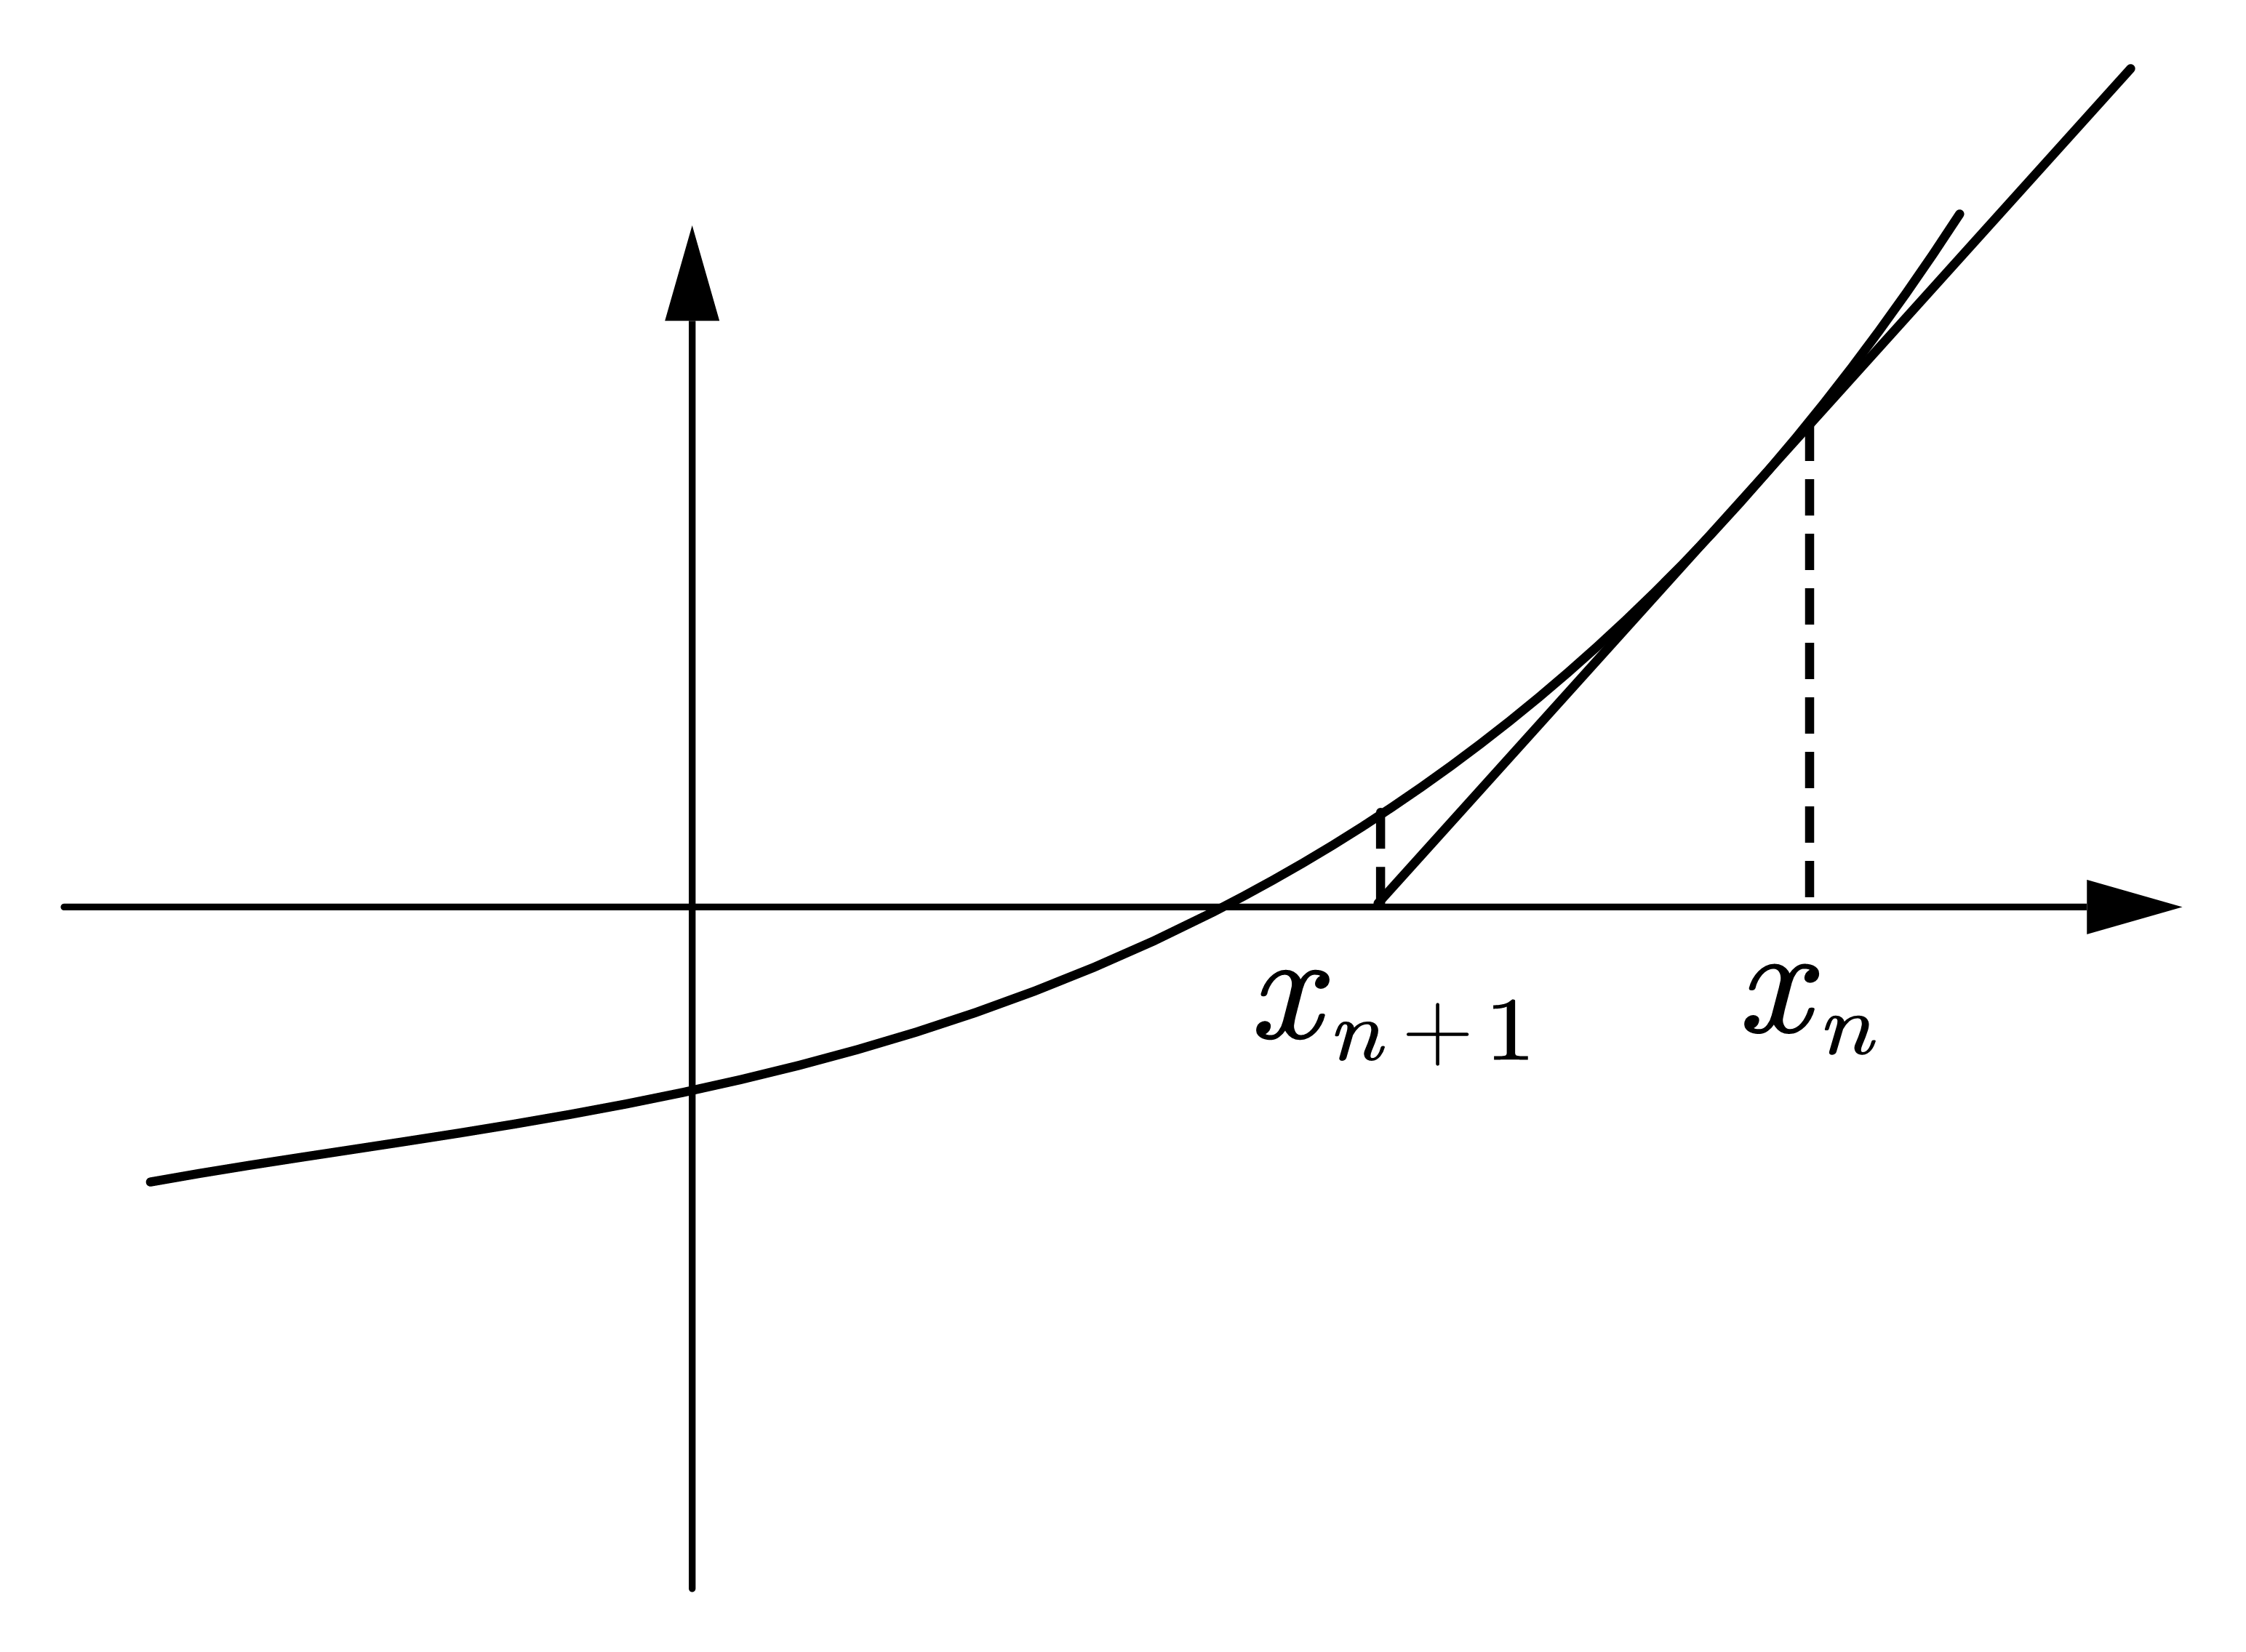
\includegraphics[width=8cm]{figure/Newton1D.png}
\end{center}

迭代过程为:
$$x_{n+1}=x_n-\frac{f(x_n)}{f'(x_n)}$$


\subsubsection{Secant方法}
牛顿迭代法中需要计算梯度,如果对梯度进行近似,可以得到其它一些方法.

$$f'(x_n)\simeq \frac{f(x_n)-f(x_{n-1})}{x_n-x_{n-1}}$$

迭代方法为
$$x_{n+1}=x_n-\frac{f(x_n)(x_n-x_{n-1})}{f(x_n)-f(x_{n-1})}$$

需要2个初始点,可以任选,或者计算一次导数,后面就不再需要计算导数了.

\subsection{解多元方程组}
求矩阵逆、伪逆也可以视为求多元方程组。
\subsubsection{不动点迭代}
\paragraph*{原始方法}对于方程
$$\bx=\bm{g}(\bx),\quad \bm{g}:\Rns\rightarrow \Rns$$
原始方法就是取$\bx_0$反复迭代到收敛。一个例子是
\begin{empheq}{align*}
x_1&=\frac{2\cos(x_2x_3)+1}{6}\\
x_2&=\frac{\sqrt{x_2^2+\sin x_3+1}}{9}-\frac{\sqrt{3}}{18}\\
x_3&=-\frac{e^{-x_1x_2}}{20}-\frac{10\pi-3}{60}
\end{empheq}
精确解为$\left[\inv{2},0,-\frac{\pi}{6}\right]$。
\paragraph*{Andreson加速}\label{andreson-fixed-point}新值是旧值的加权平均,权重通过优化残差得到。

取$\bm{f}_k=\bm{g}(\bx_k)-\bx_k$为残差。再取一个整数$m$作为分量数。算法:
\begin{enumerate}
\item 初始化$\bx_0,\bx_1=G(\bx_0),F_0$,
\item 对于$k\geq 1$,取$m_k=\min\{m,k\}$,装配矩阵$F=[\bm{f}_{k-m_k},\cdots,\bm{f}_k]$,就是取旧的$m_k$个值。求解最小二乘问题:
\begin{empheq}{align*}
\min_{\balpha}\quad & \|F\balpha\|_2\\
\text{s.t.}\quad & \balpha^T\bm{1}=1
\end{empheq}
根据拉格日乘数法,有
$$2F^TF\balpha=\lambda \bm{1}$$
则有
$$\balpha=\frac{\lambda}{2}(F^TF)^{-1}\bm{1}$$
代入$\balpha^T\bm{1}=1$可解出$\lambda$,然后有
$$\balpha=\inv{\bm{1}^T(F^TF)^{-1}\bm{1}}(F^TF)^{-1}\bm{1}$$

装配矩阵$G=[\bm{g}(\bx_{k-m_k}),\cdots, \bm{g}(\bx_k)]$,则新值为
$$\bx_{k+1}=G\balpha$$

在实现时,其实每一次不需要重新组装矩阵,只要$F,G$的列是对应的即可,因此可以这样,每一新分量加入到之前的下一列,如果装满了就填到第1列,然后第2列,……。

不过迭代几次后$f_k$就会趋于0,此时$F^TF$可能为奇异阵,因此不太可靠。需要使用更稳定的算法,参考\ref{linear-min-squared-prob}。
\end{enumerate}

以二分量为例,编程可以这样:
\begin{algorithm}
\SetKwData{Left}{left}\SetKwData{This}{this}\SetKwData{Up}{up}

\KwIn{$\bx_0$}
\KwOut{$\bx_k$}
\BlankLine
Initialization:\\
\quad$\bx_1=g(\bx_0)$\\
\quad$G=[\bx_1,g(\bx_1)]$\\
\quad$F=[g(\bx_0)-\bx_0,g(\bx_1)-\bx_1]$
\BlankLine
\For{$k=2$ \KwTo $n$}{
	求解$\balpha$\\
    $i=k \mod 2$\\
    $\bx_k=G\balpha$\\
	$G[,i]=g(\bx_k)$\\
	$F[,i]=g(\bx_k)-\bx_k$\\
}
\caption{2分量Anderson不动点迭代加速}
\end{algorithm}
从实践中来看,用Anderson加速可能初期很快,但由于浮点误差,可能最终得到的误差不如直接不动点。比如某个值的精确解为0,用不动点迭代6次到达$10^{-6}$,15次到达$10^L{-17}$,用Andreson加速,可能$3$次到达$10^{-6}$,但15次后可能只到$10^{-12}$。
\paragraph*{与梯度下降的关系}从某种意义上说,梯度下降法\ref{grade_descent}也是一种不动点迭代。

我们希望求解
$$g(\btheta)=\nabla f(\btheta)=0$$
则
$$J(g(\btheta))=\nabla^2 f(\btheta)$$
而且希望在这一点处是局部极小值。

取不动点迭代
$$\btheta=\btheta-\eta g(\btheta)$$
只要步长$\eta$取得足够小,则可以确保$\|\eta J\|\leq 1$,从而可以保证收敛性。

不动点迭代中取负梯度就是为了满足局部极小值,沿着负梯度方向,函数值下降,对应局部极小值。
\subsubsection{多元牛顿法}
直接把导数换成$J$矩阵:
$$\bx_{n+1}=\bx_n-\left(J(f(\bx_n)\right)^{-1}\bx_{n}$$

\subsubsection{Chebshev方法}
在\cite{li_chebyshev-type_2011}中对这种方法有比较详细的说明,该文章还推导了求伪逆的迭代方法。

\section{无约束多元函数优化}
以下默认是最小化.而且都需要提供初始值.

\subsection{梯度下降法系列}\label{gradient-descent-series}
只需要梯度信息。
\subsubsection{原始方法}\label{grade_descent}
无约束算法.属于一种最基本的算法,其它许多算法是根据这个算法改进而来.迭代过程为
$$\bx_{n+1}=\bx_n-\gamma \Delta F(\bx)$$

$\gamma$为步长,通常需要进行一维搜索得到,可以利用前面求解一元方程组的办法.

梯度下降法的变体主要集中在如何计算梯度以及选择的步长上面,有时还需要进行一些校正.

梯度下降法的一个有趣现象是,某点处的梯度要么与起始点的梯度平行,或者正交,这与等值面的法向量就是函数的梯度有关,也就是说,下降方向是等值面的法向量。而且下一个最优点就是等值面法线(1维)与另一个等值面的切点。如下图所示:

\begin{center}
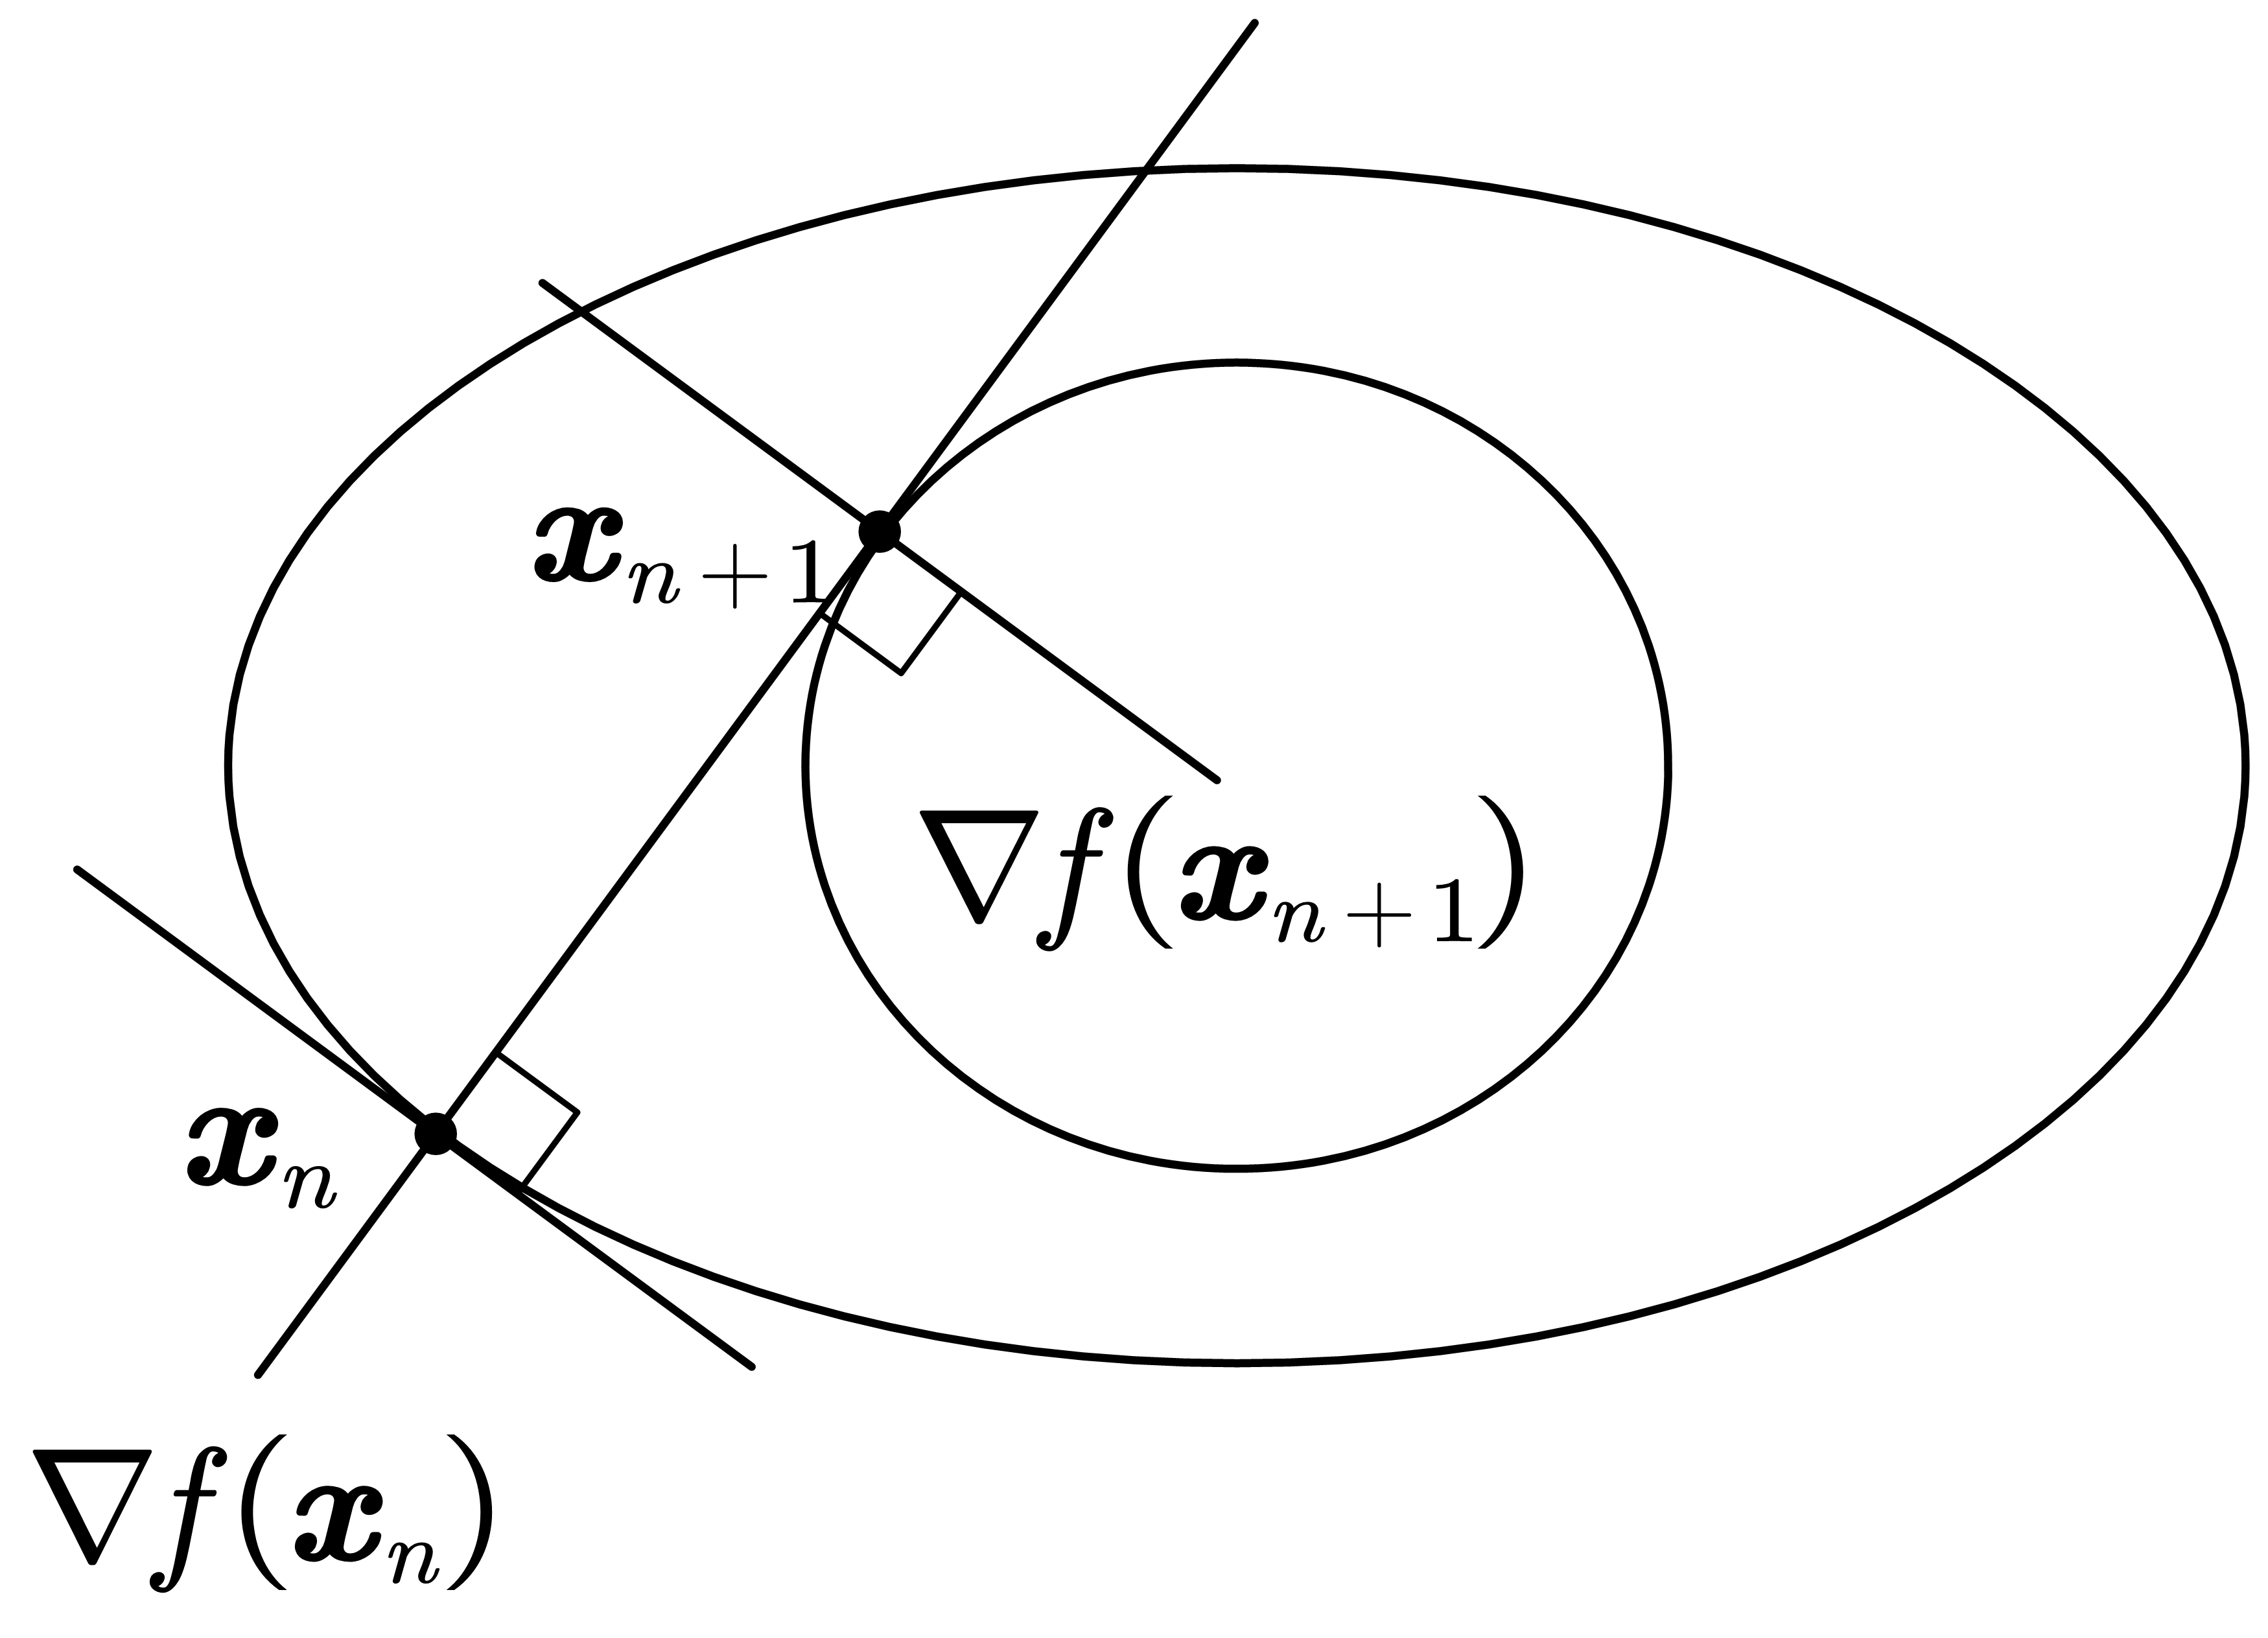
\includegraphics[width=6cm]{figure/grad_descent.png}
\end{center}

这一点也可以从迭代过程看出来,假如起始点为$\bm{x}^0$,现在进行梯度下降,则一维搜索的最优条件为
$$\pdv{f(\bx^0+\lambda \nabla f(\bx^0))}{\lambda}=\nabla f(\bx^0+\lambda \nabla f(\bx^0)))^T\nabla f(\bx^0)=\nabla f(\bx^1)^T\nabla f(\bx^0)=0$$
注意到第一次的下降方向是$\nabla f(\bx^0)$,第二次的下降方向是$\nabla f(\bx^1)$,两者内积为0,因此正交。
\subsubsection{随机梯度下降法}
对于机器学习,如果进行优化,就要计算全样本的梯度,如果每次只取一小部分甚至只取1个样本来计算,就是随机梯度下降.没有添加新的东西.不过步长现在不能再进行搜索了,只能固定,或者定期减小来稳定化.

\subsubsection{Adam}
\begin{empheq}{align*}
\bm{g}_{n}&=\nabla f(\bx_{n})	\\
\bm{m}_{n+1}&=\beta_1 \bm{m}_{n}+(1-\beta_1) \bm{g}_{n}\\
\bm{v}_{n+1}&=\beta_1 \bm{v}_{n}+(1-\beta_1) \bm{g}_{n}^2\\
\hat{\bm{m}}_{n+1}&=\frac{\bm{m}_{n}}{1-\beta_1^n}\\
\hat{\bm{v}}_{n+1}&=\frac{\bm{v}_{n}}{1-\beta_2^n}\\
\bx_{n+1}&=\bx_{n}-\frac{\alpha \hat{\bm{m}}_{n+1}}{\sqrt{\hat{\bm{v}}_{n+1}}+\varepsilon}
\end{empheq}

$\beta_1,\beta_2,\varepsilon$是预先确定的参数.通常$\beta_1,\beta_2$需要非常接近1,否则求指数后很快变成0了.原版论文的参数中,取$\beta_1=0.9,\beta_2=0.999,\varepsilon=10^{-8}$。$\alpha$就是学习率。$\bm{m}_0,\bm{v}_0$需要作为初始值给定,它们又被称为动量.注意到$\bm{m}_{n+1}$在$\beta_1=0.9$时,其中只有$1-0.9=0.1$倍直接计算的梯度,还是比较小的。

在实现时,只需要存储$\bm{m},\bm{v}$,可以通过就地修改来减少内存占用。但要看清楚,$\bm{m,v}$是自回归,不是对$\hat{\bm{m}},\hat{\bm{v}}$。另外需要注意的是迭代过程都是Elementwise计算。$n$的起始值不能为0,可以设成1。

在\cite{loshchilov2019decoupled}中提出了一种正则化方法,就是pytorch使用的\texttt{weight\_decay}。其公式是:
\begin{empheq}{align*}
\bm{g}_{n}'&=\bm{g}_n+\boxed{\lambda \bx_{n}}	\\
\bx_{n+1}'&=\bx_{n+1}-\boxed{\eta_t\lambda\bx_{n}}
\end{empheq}
$\lambda$对应decay,一般是取非常小的值。
\subsection{牛顿法系列}
\subsubsection{原始牛顿法}
\begin{empheq}{equation}
\bx^{(k+1)}=\bx^{(k)}-\nabla^2f(\bx^{(k)})^{-1}\nabla f(\bx^{(k)})
\end{empheq}
\subsubsection{拟牛顿法}
原始牛顿法需要计算$\nabla^2$的逆矩阵,这个非常难算,所以可以设法逼近它。记
\begin{empheq}{align*}
H_k&=\nabla^2f(\bx^{(k)})^{-1}\\
\bm{p}^{(k)}&=\bx^{(k+1)}-\bx^{(k)}\\
\bm{q}^{(k)}&=\nabla f(\bx^{(k+1)})-\nabla f(\bx^{(k)})
\end{empheq}

把$\nabla f(\bx^{(k)})$在$\bx^{(k+1)}$处展开后可以得到:
$$\nabla f(\bx^{(k)})=\nabla f(\bx^{(k+1)})+\nabla^2 f(\bx^{(k+1)})(\bx^{(k)}-\bx^{(k+1)})$$
变形即有
\begin{equation}
\bm{p}^{(k)}=H_{k+1}\bm{q}^{(k)}	\mtag{拟牛顿条件}
\end{equation}
取
$$H_{k+1}=H_{k}+\Delta H_{k}$$
可以用不同的方法来逼近这个$\Delta H_{k+1}$,这个矩阵也称为校正矩阵。

以下说明完整的过程:
\begin{enumerate}
\item 给定$\bx^{(0)}$计算一个初始的$H_0$,最优化$f(\bx^{(0)}-\lambda_0 H_0\nabla f(\bx^{(0)}))$得到$\lambda, x^{(1)}$.
\item 求$H_1,\bm{d}^{(1)},\lambda_1,\bx^{(2)}$。
\item 不断迭代上一步,直到停止。
\end{enumerate}

\paragraph*{秩1校正}假设矩阵的Rank是1,那么
$$\Delta H_k=\alpha_k \bz^{(k)}(\bz^{(k)})^T$$
$\alpha_k$是缩放系数。于是
\begin{empheq}{equation}\label{p-newton-rank-1}
\bm{p}^{(k)}=H_k\bm{q}^{(k)}+\alpha_k  \bz^{(k)}(\bz^{(k)})^T\bm{q}^{(k)}
\end{empheq}
这里表面上看未知数是$\alpha_k,\bz^{(k)}$,有$n+1$个,但方程是$n$个。实际上,$\alpha_k=\sign(\alpha_k)\sqrt{|\alpha_k|}^2$,所以它可以归约为$\pm 1$,因此只有$n+\inv{2}>n$个未知数,所以这个方程组是不定的,可能有多个解,即多种校正方法。

根据式\eqref{p-newton-rank-1}有
$$\bz^{(k)}=\frac{\bm{p}^{(k)}-H_k\bm{q}^{(k)}}{\alpha_k\bz^{(k)T}\bm{q}^{(k)}}$$
转置一下有:
$$\bz^{(k)}=\frac{(\bm{p}^{(k)}-H_k\bm{q}^{(k)})^T}{\alpha_k\bz^{(k)T}\bm{q}^{(k)}}$$
上两式相乘有
\begin{empheq}{equation}\label{p-newton-zzk}
\bz^{(k)}\bz^{(k)T}=\frac{(\bm{p}^{(k)}-H_k\bm{q}^{(k)})(\bm{p}^{(k)}-H_k\bm{q}^{(k)})^T}{\alpha_k^2(\bz^{(k)T}\bm{q}^{(k)})^2}
\end{empheq}

同时式\eqref{p-newton-rank-1}两边左乘$\bm{q}^{(k)T}$有
$$\bm{q}^{(k)T}(\bm{p}^{(k)}-H_k\bm{q}^{(k)})=\alpha_k(\bz^{(k)T}\bm{q}^{(k)})^2$$

这里给出了式\eqref{p-newton-zzk}的分子。所以
$$\Delta H_k=\frac{(\bm{p}^{(k)}-H_k\bm{q}^{(k)})(\bm{p}^{(k)}-H_k\bm{q}^{(k)})^T}{\bm{q}^{(k)T}(\bm{p}^{(k)}-H_k\bm{q}^{(k)})}$$

\paragraph*{DFP方法}公式如下:
\begin{empheq}{equation}\label{p-newton-DFP}
\Delta H_k=\frac{\bm{p}^{(k)}\bm{p}^{(k)T}}{\bm{p}^{(k)T}\bm{q}^{(k)}}-\frac{H_k\bm{q}^{(k)}\bm{q}^{(k)T}}{\bm{q}^{(k)}H_k\bm{q}^{(k)T}}
\end{empheq}

\paragraph*{BFGS}公式如下
\begin{empheq}{align}\label{p-newton-BFGS}
\Delta H_k&=\left(1+\frac{\bm{q}^{(k)T}H_k\bm{q}^{(k)}}{\beta}\right)\frac{\bm{p}^{(k)}\bm{p}^{(k)T}}{\beta}-\frac{\bm{p}^{(k)}\bm{q}^{(k)T}H_k+H_k\bm{q}^{(k)}\bm{p}^{(k)T}}{\beta}\\
\beta_k&=\bm{p}^{(k)T}\bm{q}^{(k)}
\end{empheq}

取
$$\bm{q}^{(k)}=B_{k+1}\bm{p}^{(k)}$$
然后利用DFP方法\eqref{p-newton-DFP}可以得到$B_{k}$的递推公式,再求逆:
$$H_{k+1}=B_{k+1}^{-1}$$
即可得到BFGS方法\eqref{p-newton-BFGS}。
\subsection{共轭梯度法}
\subsubsection{概念}
\begin{definition}[共轭梯度]\label{conjugate-gradient}
$A$为正定矩阵,如果$\bm{d}^{(1)},\bm{d}^{(2)}\in\mathbb{R}^n$满足
$$\bm{d}^{(1)T}A\bm{d}^{(2)}=0$$
称$\bm{d}^{(1)},\bm{d}^{(2)}$关于$A$共轭(正交)。
\end{definition}
%取Cholesky分解$A=LL^{T}$
以下给出一些关于共轭梯度有关的例子:
\begin{example}
$A$为一正定矩阵,$\bm{p}^{(i)},i\in\{1,\cdots,n\}$关于$A$共轭,给定某$\bx\in\mathbb{R}^n$,试求$\bx$在基$\bm{p}^{(i)}$下的坐标。
\end{example}
\begin{solution}
假设$\bx=\sum \alpha_i \bm{p}^{(i)}$,则
$$\bm{p}^{(i)}A\bx=\alpha_i\bm{p}^{(i)}A\bm{p}^{(i)}$$
于是
$$\alpha_i=\frac{\bm{p}^{(i)}A\bx}{\bm{p}^{(i)}A\bm{p}^{(i)}}$$
\end{solution}
\subsubsection{计算过程}
基本原理是每隔$n$次用最速下降方向“重启”,否则用其它方法对搜索方向校正。

计算步骤如下:
\begin{enumerate}
\item 给定初始点$\bx^{(1)}$,取$\by^{(1)}=\bx^{(1)},\bm{d}^{(1)}=-\nabla f(\by^{(1)}),k=j=1$。
\item\label{conjudate-gradient-1d-search} 假如$\|\nabla f(\by^{(1)})\|\leq \varepsilon$,停止。否则进行一维搜索,求解
$$\min_{\lambda \geq 0}f(\by^{(j)}+\lambda_j \bm{d}^{(j)})$$
得到$\by^{(j+1)}$。
\item 如果$j<n$, 进行步骤\ref{conjudate-gradient-calibrate};否则,进行步骤\ref{conjudate-gradient-restart}(重置)。
\item\label{conjudate-gradient-calibrate}  校正方向。取$\bm{d}^{(j+1)}=-\nabla f(\by^{(j+1)})+\beta_j \bm{d}^{(j)}$,其中
$$\beta_j=\frac{\|\nabla f(\bm{y}^{(j+1)})\|^2}{\|\nabla f(\bm{y}^{(j)})\|^2}$$
取$j\coloneqq j+1$。
\item\label{conjudate-gradient-restart}取$\bx^{(k+1)}=\by^{(n+1)},\by^{(1)}=\bx^{(k+1)},\bm{d}^{(1)}=-\nabla f(\by^{(1)}),j=1,k\coloneqq k+1$,转步骤\ref{conjudate-gradient-1d-search}。
\end{enumerate}
$k$是全局迭代次数。
\subsection{信赖域法}

\subsection{各种方法的比较}

\section{约束多元函数优化}
\subsection{最小二乘}
\subsubsection{线性约束最小二乘}\label{linear-min-squared-prob}
在不动点迭代的Andreson方法\ref{andreson-fixed-point}中需要求解以下问题:
\begin{empheq}{align*}
\min_{\balpha}\quad & \|F\balpha\|_2,F\in\mathbb{R}^{n\times k}\\
\text{s.t.}\quad & \balpha^T\bm{1}=1
\end{empheq}
如果直接求解的话,由于$F^TF$通常条件数很大,不能求逆,需要更稳定的方法。以下说明一种基于零空间的方法:
\paragraph*{Null-space方法},首先取$\bm{v}=[0,0,\cdots,1]^T\in\mathbb{R}^{k}$,假设存在满秩矩阵$V\in\mathbb{R}^{k\times (k-1)}$满足$\bm{1}^TV=\bm{0}$,则可以令$\balpha=\bm{v}+V\bm{\gamma}$,原问题转换为一个无约束优化问题:
\begin{empheq}{align*}
\min_{\bm{\gamma}}\quad & \|F(\bm{v}+V\bm{\gamma})\balpha\|_2=\bm{d}_k+FV\bm{\gamma}
\end{empheq}
$\bm{d}_k$就是$F$的最后一列。一阶条件为
$$(DV)^TDV\bm{\gamma}=-(DV)^TD\bm{\gamma}$$
$(DV)^T$条件数也还是很大,可以使用QR分解,取$DV=QR$,则一阶条件变成
$$R\bm{\gamma}=-Q^T\bm{d}_k$$
求解上式即可。最后$\bm{\alpha}=\bm{v}+V\bm{\gamma}$。
\subsection{可行方向法}
\subsubsection{Zoutendijk法}
\paragraph*{线性约束}求解线性等式、不等式约束问题\ref{constrained-lin-eq-neq}的Zoutendijk方法如下:
\begin{enumerate}
\item 给定初始点$\bx^{(1)}$,取$k=1$。
\item\label{zoutendijk-linear-2}把不等式约束条件分解为起作用与不起作用约束:
\begin{empheq}{equation}
A=\begin{bmatrix}
A_1\\A_2
\end{bmatrix},\bm{b}=\begin{bmatrix}
\bm{b}_1\\\bm{b}_2
\end{bmatrix}
\end{empheq}
其中$A_1\bm{x}^{(k)}=\bm{b}_1,A_2\bm{x}^{(k)}\geq \bm{b}_2$。需要强调的是,$\bx\geq \bm{0}$也属于约束条件,不要忘记。计算$\nabla f(\bx^{(k)})$。
\item 求解线性规划:
\begin{empheq}{equation}
\begin{aligned}
&\min && \nabla f(\bx^{(k)})^T\bm{d}\\
	&\text{s.t. } && A_1\bm{d}\geq \bm{0}\\
	& && E\bm{d}=\bm{0}\\
	& && -1\leq \bm{d}\leq 1
\end{aligned}
\end{empheq}
得到最优解$\bm{d}^{(k)}$。
\item 如果$\nabla f(\bx^{(k)})^T\bm{d}^{(k)}=0$。停止计算,得到K-T点。否则进行下一步。
\item\label{zoutendijk-lin-1d-search} 一维搜索。首先计算范围。取
\begin{empheq}{align}
\hat{\bm{b}}&=\bm{b}_2-A_2\bx^{(k)}\\
\hat{\bm{d}}&=A_2\bm{d}^{(k)}
\end{empheq}
然后令
\begin{empheq}{equation}
\lambda_{\max}=\begin{cases}
\min\  \left\{\frac{\hat{b}_i}{\hat{d}_i}\rvert \hat{d}_i<0\right\}& \hat{\bm{d}}\ngeq \bm{0}\\
\infty & \hat{\bm{d}}\geq \bm{0}
\end{cases}
\end{empheq}
$\hat{\bm{b}}$实际上是不起作用约束条件的“残差”,限定了调整范围。

进行一维搜索
\begin{empheq}{equation}
\min_{\lambda\in [0,\lambda_{\max}]} f(\bm{x}^{(k)}+\lambda \bm{d}^{(k)})
\end{empheq}
得到最优解$\lambda_k$,同时计算$\bx^{(k+1)}$。这里在计算时不要忘记$\lambda_{\max}$。
\item 取$k\coloneqq k+1$,返回\ref{zoutendijk-linear-2}。
\end{enumerate}


\subsubsection{梯度投影法系列}
\paragraph*{基本梯度投影法}
属于最速下降法的推广。求解线性等式、不等式约束问题\ref{constrained-lin-eq-neq}的基本梯度投影方法如下:
\begin{enumerate}
 \item 给定初始点$\bx^{(1)}$,取$k=1$。
\item\label{gradient-project-linear-2}把不等式约束条件分解为起作用与不起作用约束:
\begin{empheq}{equation}
	A=\begin{bmatrix}
		A_1\\A_2
	\end{bmatrix},\bm{b}=\begin{bmatrix}
		\bm{b}_1\\\bm{b}_2
	\end{bmatrix}
\end{empheq}
其中$A_1\bm{x}^{(k)}=\bm{b}_1,A_2\bm{x}^{(k)}\geq \bm{b}_2$。
\item\label{gradient-project-linear-3} 令
\begin{empheq}{align*}
M&=\begin{bmatrix}
A_1\\E
\end{bmatrix}\\
P&=\begin{cases}
I & M\in \emptyset\\
I-M^T(MM^T)^{-1}M & \text{否则}
\end{cases}
\end{empheq}
\item 计算下降方法。令$\bm{d}^{(k)}=-P\nabla f(\bx^{(k)})$。如果$\bm{d}^{(k)}\neq \bm{0}$,转步骤\ref{gradient-project-linear-6};如果$\bm{d}^{(k)}=0$,转步骤\ref{gradient-project-linear-5}。
\item\label{gradient-project-linear-5} 如果$M$空,则停止计算。否则令
$$W=(MM^T)^{-1}M\nabla f(\bx^{(k)})=\begin{bmatrix}
	\bm{u}\\\bm{v}
\end{bmatrix}$$
如果$\bm{u}\geq \bm{0}$,停止计算。如果包含负分量,取一个负分量$u_j$,去掉$A_1$中$u_j$对应的行,返回步骤\ref{gradient-project-linear-3}。
\item\label{gradient-project-linear-6} 一维搜索。这一步与Zoutendijk法中步骤\ref{zoutendijk-lin-1d-search}相同。
\item 取$k\coloneqq k+1$,返回\ref{gradient-project-linear-2}。
\end{enumerate}
\paragraph*{Frank-Wolfe方法}属于梯度投影法的一个变种。求解线性等式约束问题\ref{constrained-lin-eq}的Frank-Wolfe方法如下。

以下记$S=\{\bx|A\bx=\bm{b},\bx\geq \bm{0}\}$,即线性约束的可行域。

\begin{enumerate}
 \item 给定初始点$\bx^{(1)}$,取$k=1$。
 \item\label{frank-wolfe-lin-linear} 求解线性规划:
 \begin{empheq}{equation}
 \min_{\bx\in S} \nabla f(\bx^{(k)})^T\bx
 \end{empheq}
得到最优解$\by^{(k)}$。
\item 如果$\nabla f(\bx^{(k)})^T(\by^{(k)}-\bx^{(k)})\leq \varepsilon$,停止计算。否则进行下一步。
\item\label{frank-wolfe-lin-1d} 从$\bx^{(k)}$出发,沿方向$\by^{(k)}-\bx^{(k)}$在线段$\by^{(k)},\bx^{(k)}$上进行一维搜索:
\begin{empheq}{equation}
\min_{\lambda in [0,1]} f(\bx^{(k)}+\lambda (\by^{(k)}-\bx^{(k)}))
\end{empheq}
得到$\lambda_k$。
\item 更新
$$\bx^{(k+1)}=\bx^{(k+1)}+\lambda_k (\by^{(k)}-\bx^{(k)})$$返回步骤\ref{frank-wolfe-lin-linear}。
\end{enumerate}
注意在以上步骤\ref{frank-wolfe-lin-1d}进行一维搜索时,不需要计算上界,上界是已知的,即1。

\subsection{罚函数法}
\subsubsection{基本原理}
罚函数法在Matlab的\texttt{solve}中有应用(Interior Point算法)。实质是把约束条件整合进目标函数。于是可以当成一个无约束问题来做,跟多目标优化很像。分为外点与内点罚函数法。前者的搜索空间是在可行域外部,不断靠近可行域;而后者的搜索空间是在可行域内部。对于等式约束,可行域内部是"空的",所以此时不能用原始的内点法。

限定搜索空间在内部是通过障碍函数$G(\bx,r)$实现的,比如在内点法中,定义为
$$G(\bx,r)=f(\bx)+rB(\bx)$$
当$\bx$趋于边界(具体地是$g_i(\bx)\rightarrow 0^+$,一般要求约束条件形如$\bm{g}(\bx)\geq \bm{0}$)时,$B(\bx)\rightarrow +\infty$。常见的两种函数为
\begin{empheq}{align*}
B(\bx)&=\sum_{i=1}^{m}\inv{g_i(\bx)}\\
B(\bx)&=-\sum_{i=1}^{m}\log g_i(\bx)
\end{empheq}
令$r\rightarrow 0$,相当于极小化$f$,同时由于$B$函数的趋于无穷大的限制,使得解尽可能靠近边界,从而趋近于最优解。

外点法是类似的,其目标函数是
\begin{empheq}{align*}
F(\bx,\sigma)&=f(\bx)+rP(\bx)\\
P(\bx)&=\sum_{i=1}^{m}\phi(g_i(\bx))+\sum_{i=1}^{n}\varphi(h_i(\bx))
\end{empheq}
$\sigma$为罚因子,通常要取得大一些。$\phi$和$\varphi$通常取为
\begin{empheq}{align*}
\phi&=\left[\max\{0,-g_i(\bx)\}\right]^{\alpha}\\
\varphi&=\|h_i(\bx)\|^\beta
\end{empheq}
一般来说$\alpha=\beta=2$,就是2-范数。而且可以看出$\phi$里面是$\ReLU$函数。外点法的含义是很明显的,就是解在可行域内部时没有惩罚,在外部时有很大的惩罚。

令$r\rightarrow \infty$,可以得到解析解。
\subsubsection{外点罚函数法}
\begin{example}
\begin{empheq}{equation}
\begin{aligned}
\min\ & (x_1-3)^2+(x_2-2)^2\\
\text{s.t. } & x_1+x_2=4
\end{aligned}
\end{empheq}
\end{example}

\begin{solution}
取目标函数
$$f(x_1,x_2)=(x_1-3)^2+(x_2-2)^2+\sigma(x_1+x_2-4)^2$$
根据一阶条件,解一个线性方程组得到:
$$\bx=\frac{1}{2\sigma+1}\begin{bmatrix}
5\sigma+3\\3\sigma+2
\end{bmatrix}$$
令$\sigma\rightarrow \infty $,有
$$\bx=\begin{bmatrix}
\frac{5}{2}\\\frac{3}{2}
\end{bmatrix}$$
\end{solution}

\subsubsection{内点罚函数法}
\begin{example}
	\begin{empheq}{equation}
		\begin{aligned}
			\min\ & \inv{12}(x_1+1)^3+x_2\\
			\text{s.t. } & x_1\geq 1,x_2\geq 0
		\end{aligned}
	\end{empheq}
\end{example}

\begin{solution}
取目标函数:
$$G(\bx,r)=\inv{12}(x_1+1)^3+x_2+r\left(\inv{x_1-1}+\inv{x_2}\right)$$

由一阶最优性条件有:
$$\bx=\begin{bmatrix}
\sqrt{1+2\sqrt{r}}\\
\sqrt{r}
\end{bmatrix}$$
令$r\rightarrow 0$,有
$$\bx=\begin{bmatrix}
	\sqrt{1}\\
	\sqrt{0}
\end{bmatrix}$$
\end{solution}
\chapter{整数与混合整数规划}
\chapter{全局优化}
\chapter{多目标优化}

\chapter{微分方程的数值算法}\label{ode-numeric}

\section{常微分方程}
\subsection{常微分方程的一般形式}
\subsubsection{主方程}
$n$阶线性常微分方程的一般形式为
\begin{empheq}{equation}
\sum_{k=1}^n a_(t,\bx)\odv[order=k]{\bx}{t}=f(t,\bx,\bx',\cdots)
\end{empheq}

线性是指为左边为导数的线性组合(系数可以是常系数,也可以是函数)。对于高阶的方程,可以通过引入额外变量的方式降阶。比如对于一元二阶线性常微分方程
$$\ddot{x}+a\dot{x}+by=f(t,x)$$
引入$x_1=x,x_2=\dot{x_1}$,则原方程可化为二元一阶线性常微分方程:
\begin{empheq}[left=\empheqlbrace]{align}
\dot{x_1}&=\dot{x}=x_2\\
\dot{x_2}&=\dot{x_1}=-ax_2-bx_1+f(t,x)
\end{empheq}

又比如非常系数的线性常微分方程也可以降阶:
$$\ddot{x}+(\sin t) \dot{x}=\cos x\implies \begin{cases}
\dot{x_1}&=\dot{x}=x_2\\
\dot{x_2}&=\dot{x_1}=-\sin t x_2+\cos x
\end{cases}$$

所以$n$阶线性常微分方程的一般形式可以表述为:
\begin{empheq}{equation}\label{1st-order-1-ode}
\dot{\bx}=\pdv{\bx}{t}=f(t,\bx) \quad \by\in\Rns
\end{empheq}
即对应一个$n$元一阶线性常微分方程组。
\subsubsection{边界条件}
\paragraph*{初值条件}给定初始时刻的值:
$$\bx(0)=\bx_0$$
对应的问题叫初值问题。初值问题适合用积分法,从初始时刻一步一步往后推。高阶方程,需要给定低阶初始导数值,比如二阶问题,要给出$\bx(0),\dot{\bx}(0)$。

初值问题适合积分法。
\paragraph*{边值问题}给定两个边界点的值
$$\bx(0)=\bx_0,\bx(T)=\bx_T$$
对应边值问题。注意,一元一阶常微分方程只有边值问题。初值问题至少需要二阶才有。

一个二阶一元方程,给定边值$x(0),x(T)$。

边值问题适合差分法。
\subsection{一元一阶线性常微分方程}
\subsubsection{积分法原理}
对于问题\eqref{1st-order-1-ode},并且假定为初值问题。按照积分的法则:
$$x_{n+1}=x_n+\int_{t_n}^{t_{n+1}} f(t,x(t))\dif t$$
右边可以用多种方法逼近。

\subsubsection{简单均值逼近}
\paragraph*{一阶时间差分}
原方程左边可以用最简单的差分逼近:
\begin{empheq}{align}
\dot{x}_n&\approx \frac{x_{n+1}-x_{n}}{h}
\end{empheq}
高阶差分格式可以参考\ref{diff-int-finite-difference}。
\paragraph*{显式Euler方法}原方程右边可以用$f(t_n,x_n)$或者$f(t_{n+1},x_{n+1})$。
就是用前一时刻的导数来逼近增量:
$$\frac{x_{n+1}-x_n}{h}=f(t_n,x_n)\implies x_{n+1}=x_n+hf(t_n,x_n)$$
可以递推计算。对应于用$t_n$处的函数值代替被积函数平均值。

\paragraph*{隐式Euler方法}用下一点处的导数逼近右边:
$$\frac{x_{n+1}-x_n}{h}=f(t_{n+1},x_{n+1})\implies x_{n+1}=x_n+hf(t_{n+1},x_{n+1})$$
显然需要解方程。性能比显式方法好。对应于用$t_{n+1}$处的函数值代替被积函数平均值。

\paragraph*{Crank-Nicolson格式}用前一时间与后一时刻的加权的方式逼近原方程右边:
\begin{empheq}{align}
&\frac{x_{n+1}-x_n}{h}=\theta f(t_{n},x_{n})+(1-\theta)f(t_{n+1},x_{n+1})\\
\implies &x_{n+1}=x_n+h(\theta f(t_{n},x_{n})+(1-\theta)f(t_{n+1},x_{n+1}))
\end{empheq}
取$\theta=\inv{2}$时,叫Crank-Nicolson格式,它是隐式方法,对应于积分的梯形法则。

\paragraph*{Predictor-Corrector校正}\label{ode-predictor-corrector}以显式Euler方法为例,先得到预测值$x_{n+1}^0=x_n+hf_n=x_n+hf(t_n,x_n)$,然后得到$f_{n+1}^0=f(t_{n+1},x_{n+1}^0)$,则根据梯形规则,预测值为
$$x_{n+1}^1=x_n+\frac{h}{2}(f_n+f_{n+1}^0)$$
这个过程可以执行多次:
\begin{empheq}{align}
x_{n+1}^0&=x_n+hf(t_n,x_n)\\
f_{n+1}^k&=f(t_{n+1},x_{n+1}^{k-1})\\
x_{n+1}^k&=x_n+\frac{h}{2}(f_n+f_{n+1}^k)
\end{empheq}
如果迭代到收敛,它可以与隐式方法具有一样的性能。以上这个过程,相当于通过不动点迭代求解
$$x_{n+1}=x_n+\frac{h}{2}(f(t_n,x_n)+f(t_{n+1},x_{n+1}))$$
相当于隐式积分法了。

\subsection{二阶一元常线性微分方程}
\subsubsection{差分法}
对于二阶一元常线性微分方程
$$a\ddot{x}+b\dot{x}=f(t,x)$$
假定为边值问题,即将时间段分成$N+1$个区间,给定$x_0,x_{N+1}$,待求解的是$[x_1,\cdots,x_N]'$,即有$N$个变量。

\paragraph*{差分格式}二阶导数取中心差分:
$$\ddot{x}=\frac{x_{t+1}-2x_t+x_{t-1}}{h^2}$$
一阶导数取前向差分。
\paragraph*{方程组}采用隐式Euler方法,则可得到$N$个方程组:
\begin{empheq}{align}
a\frac{x_{2}-2x_1+x_{0}}{h^2}+b\frac{x_1-x_0}{h}&=f(t_1,x_1)\\
a\frac{x_{3}-2x_2+x_{1}}{h^2}+b\frac{x_2-x_1}{h}&=f(t_2,x_2)\\
a\frac{x_{4}-2x_3+x_{2}}{h^2}+b\frac{x_3-x_2}{h}&=f(t_3,x_3)\\
\cdots &\cdots\\
a\frac{x_{N+1}-2x_N+x_{N-1}}{h^2}+b\frac{x_N-x_{N-1}}{h}&=f(t_{N},x_N)
\end{empheq}
这是一个非线性方程组。如果$f$与$\bx$无关,即只与$t$有关,则上面的方程组对应一个线性方程组:
\begin{empheq}{align}
\begin{bmatrix}
-2+\frac{b}{a}h & 1 & & & &  \\
1-\frac{b}{a}h & -2+\frac{b}{a}h&1 & \cdots & & \\
 & 1-\frac{b}{a}h & -2+\frac{b}{a}h&1 & & \\
&  & & \cdots& & \\
 &  & & & 1-\frac{b}{a}h&-2+\frac{b}{a}h 
\end{bmatrix}
\begin{bmatrix}
x_1\\
x_2\\
x_3\\
\cdots\\
x_N
\end{bmatrix}=\frac{h^2}{a}\begin{bmatrix}
f(t_1)\\
f(t_2)\\
f(t_3)\\
\cdots\\
f(t_N)
\end{bmatrix}+\begin{bmatrix}
1+\frac{b}{a}hx_0\\
0\\
0\\
\cdots\\
-x_{N+1}
\end{bmatrix}
\end{empheq}
对应
$$A\bx=F$$
可以看出系数矩阵为三对角矩阵,对角线上元素相同,上对角线全为1,下对角线也相同。

\subsection{其它常微分方程}
\subsubsection{多元一阶常微分方程}

\section{偏微分方程}
\subsection{差分法}

\subsection{有限元方法}
\subsubsection{弱形式}
\paragraph*{弱形式的导出}
有限元方法的起点是PDE的弱形式,也叫变分形式。考虑一个泊松方程:
$$-\Delta u(x,y)=f(x,y)$$
给两边乘上一个测试函数$v$,再在全区域上积分,即可得到弱形式:
\begin{empheq}{align}
\iint_{\Omega}(-\Delta u-f)v\dif S=\iint_{\Omega} \nabla u\cdot \nabla v - fv\dif S=0
\end{empheq}
这里用到了格林公式\ref{green-formula}。这个方程应该对所有$v$成立。说它是弱形式,是因为原方程是在每点成立,而这个方程是在全区域的积分下成立,因此强形式的解必然满足弱形式,但弱形式的解不一定满足强形式。
\subsection{有限体积法}

\subsection{同伦分析法}

\chapter{组合与动态优化}

\section{确定型动态优化}
\subsection{等式约束、无限期、贴现}
\subsubsection{问题形式}
考虑一个一般的动态决策问题:
\begin{empheq}{align}\label{dynamic-decision-problem}
\max_{\{\bx_t\}_0^\infty}&\quad\sum_{t=0}^{\infty}\beta^t\varphi(\bx_t,\by_t)\\
\text{s.t.}&\quad \bx_t\in\Gamma(\by_t),\by_{t+1}=F(\bx_t,\by_t)\\
&\quad\bx_t\in\mathbb{R}^n,\by_t\in\mathbb{R}^k,\by_0\text{已知}
\end{empheq}
$\beta$为贴现率,$\bx$为控制变量(决策),$\by$为状态变量。约束条件的含义是说,本期的决策与本期的状态$y_t$有关,下一期的状态与本期的状态与决策有关。

这个问题出现在高级宏观经济学、强化学习、控制论中。
\subsubsection{拉格朗日函数法}
\paragraph*{一阶条件}
问题\ref{dynamic-decision-problem}的拉格朗日函数为:
\begin{empheq}{equation}
\mathcal{L}(\bx_t,\by_{t+1})=\sum_{t=0}^{\infty}\beta^t\varphi(\bx_t,\by_t)+\sum_{t=0}^{\infty}\blambda_t^T(\by_{t+1}-F(\bx_t,\by_t))
\end{empheq}
可以给出一阶条件为:
\begin{empheq}{align}
\pdv{\mathcal{L}}{\bx_t}&=\beta^t\pdv{\varphi}{\bx_t}-\left(\pdv{F(\bx_t,\by_t)}{\bx_t}\right)^T\bm{\lambda}_t=\bm{0}\\
\pdv{\mathcal{L}}{\by_{t+1}}&=\blambda_t+\beta^{t+1}\pdv{\varphi(\bx_t,\by_t)}{\by_{t+1}}-\left(\pdv{F(\bx_{t+1},\by_{t+1})}{\by_{t+1}}\right)^T\bm{\lambda}_{t+1}=0\\
&\by_{t+1}-F(\bx_t,\by_t)=0
\end{empheq}

\paragraph*{消费者效用优化}考虑如下的消费者效用优化。式中$c_t$为消费,$k_t$为资本。
\begin{empheq}{align}
\max_{c_t}\quad &\sum_{t=0}^{\infty} \beta^tu(c_t)\\
\text{s.t.}\quad & k_{t+1}=f(k_t)-c_t
\end{empheq}

代入上面的一阶条件有:
\begin{empheq}{align}
\beta^tu'(c_t)+\lambda_t&=0\\
\lambda_t-f'(k_{t+1})\lambda_{t+1}&=0
\end{empheq}
根据第一式有:$\lambda_{t+1}=-\beta^{t+1}u'(c_{t+1})$,代入第二式有:
\begin{empheq}{equation}
-\beta^t u'(c_t)+f'(k_{t+1})\beta^{t+1}u'(c_{t+1})\implies \beta u'(c_{t+1})f'(k_{t+1})=u'(c_t)
\end{empheq}
再代入$c_t=f(k_t)-k_{t+1}$,即有:
$$\beta u'(f(k_{t+1})-k_{t+2})f'(k_{t+1})=u'(f(k_t)-k_{t+1})$$
这就是\emph{资本积累方程},它是二阶一个差分方程。

\subsubsection{动态规划法}
\paragraph*{贝尔曼准则}
贝尔曼准则是说,无论初始状态$\by_0$与初始决策$\bx_0$如何,余下的决策必然相对状态$\by_1$构成最优决策。记
$$V(\by_k)=\max_{\{\bx_t\}_k^\infty}\ \sum_{t=k}^{\infty}\beta^t\varphi(\bx_t,\by_t)$$
表示在$k$期状态为$\by_k$的情况下进行最优决策得到的收益 。

则依据贝尔曼准则,原问题等价于贝尔曼方程:
\begin{empheq}{align}\label{dynamic-decision-bellman-equation}
V(\by_0)=\max_{\bx_0}&\  \varphi(\by_0,\bx_0)+\beta V(\by_1)\\
\text{s.t.}&\ \by_{1}=F(\by_0,\bx_0)
\end{empheq}

这里有一个小问题,是先无条件承认贝尔曼准则,从而得到贝尔曼方程;还是先得到贝尔曼方程,再总结为贝尔曼准则呢?应该是后者。可以这样考虑,假设我们已经做了决策$\bx_0$,那么剩下的决策必然达到局部最优,即对应贝尔曼方程。

\paragraph*{Bellman方程的一阶最优条件}
假如问题是连续的,则问题\cref{dynamic-decision-bellman-equation}在$t$时期对应拉格朗日函数为:
$$\mathcal{L}(\bx_t,\by_{t+1})=\varphi(\bx_t,\by_t)+\beta V(\by_{t+1})+\lambda_t^T(\by_{t+1}-F(\bx_t,\by_t))$$

一阶最优条件为:
\begin{empheq}{align}\label{dymaic-decision-bellman-eq-FOC}
\pdv{\mathcal{L}}{\bx_t}&=\pdv{\varphi(\bx_t,\by_t)}{\bx_t}+\left(\pdv{F(\bx_t,\by_t)}{\bx_t}\right)^T\bm{\lambda}_t=\bm{0}\\
\pdv{\mathcal{L}}{\by_{t+1}}&=\beta\pdv{V(\by_{t+1})}{\by_{t+1}}+\bm{\lambda}_t=0
\end{empheq}
注意我们不能只考虑$\bx_t$,因为$\bx_t$会影响后面的决策。


\paragraph*{包络引理}
\begin{empheq}{equation}
\odv{V(\by_t)}{\by_t}=\pdv{\mathcal{L}}{\by_t}=\pdv{\varphi(\bx_t,\by_t)}{\by_t}+\left(\pdv{F(\bx_t,\by_t)}{\by_t}\right)^T\bm{\lambda}_t
\end{empheq}
注意$\by_t$本身不是$\mathcal{L}$的直接参数。根据全微分展开$\mathcal{L}$,再取最优解时对决策变量的导数为0,可以得到这个等式。

\subsection{一般约束、有限期、一般}
\subsubsection{问题形式}
考虑一个一般化的有限期动态优化问题:
\begin{empheq}{align}\label{dynamic-decision-problem-gcons-finite-g}
\max_{\{\bx_t\}_0^T}&\quad\sum_{t=0}^{T}\varphi(\bx_t,\by_t)\\
\text{s.t.}&\quad \bx_t\in\Gamma(\by_t),\by_{t+1}=F(\bx_t,\by_t)\\
&\quad G(\by_t,\bx_t)\geq 0\\
&\quad\bx_t\in\mathbb{R}^n,\by_t\in\mathbb{R}^k
\end{empheq}
上面的不等式约束通常用来表示某些值不能非负,比如净资产不为负。
\subsubsection{NLP法}
\paragraph*{最大值原理}有限期问题的最大好处是可以直接当成静态优化,即一般的NLP问题来做,待求解变量变量为$\bx_0,\bx_1,\cdots,\bx_T$,每个时间点可以构造相应的约束条件。这样便于使用数值优化。

其最优性条件参考凸优化章节中的中的内容\ref{nlp-cons-opt-FOC}。

\section{不确定型动态优化}


\chapter{控制论}

\chapter{计算理论}

\section{理解计算}
\subsection{计算的一般模式}
下图展示了计算的一般模式:

\begin{center}
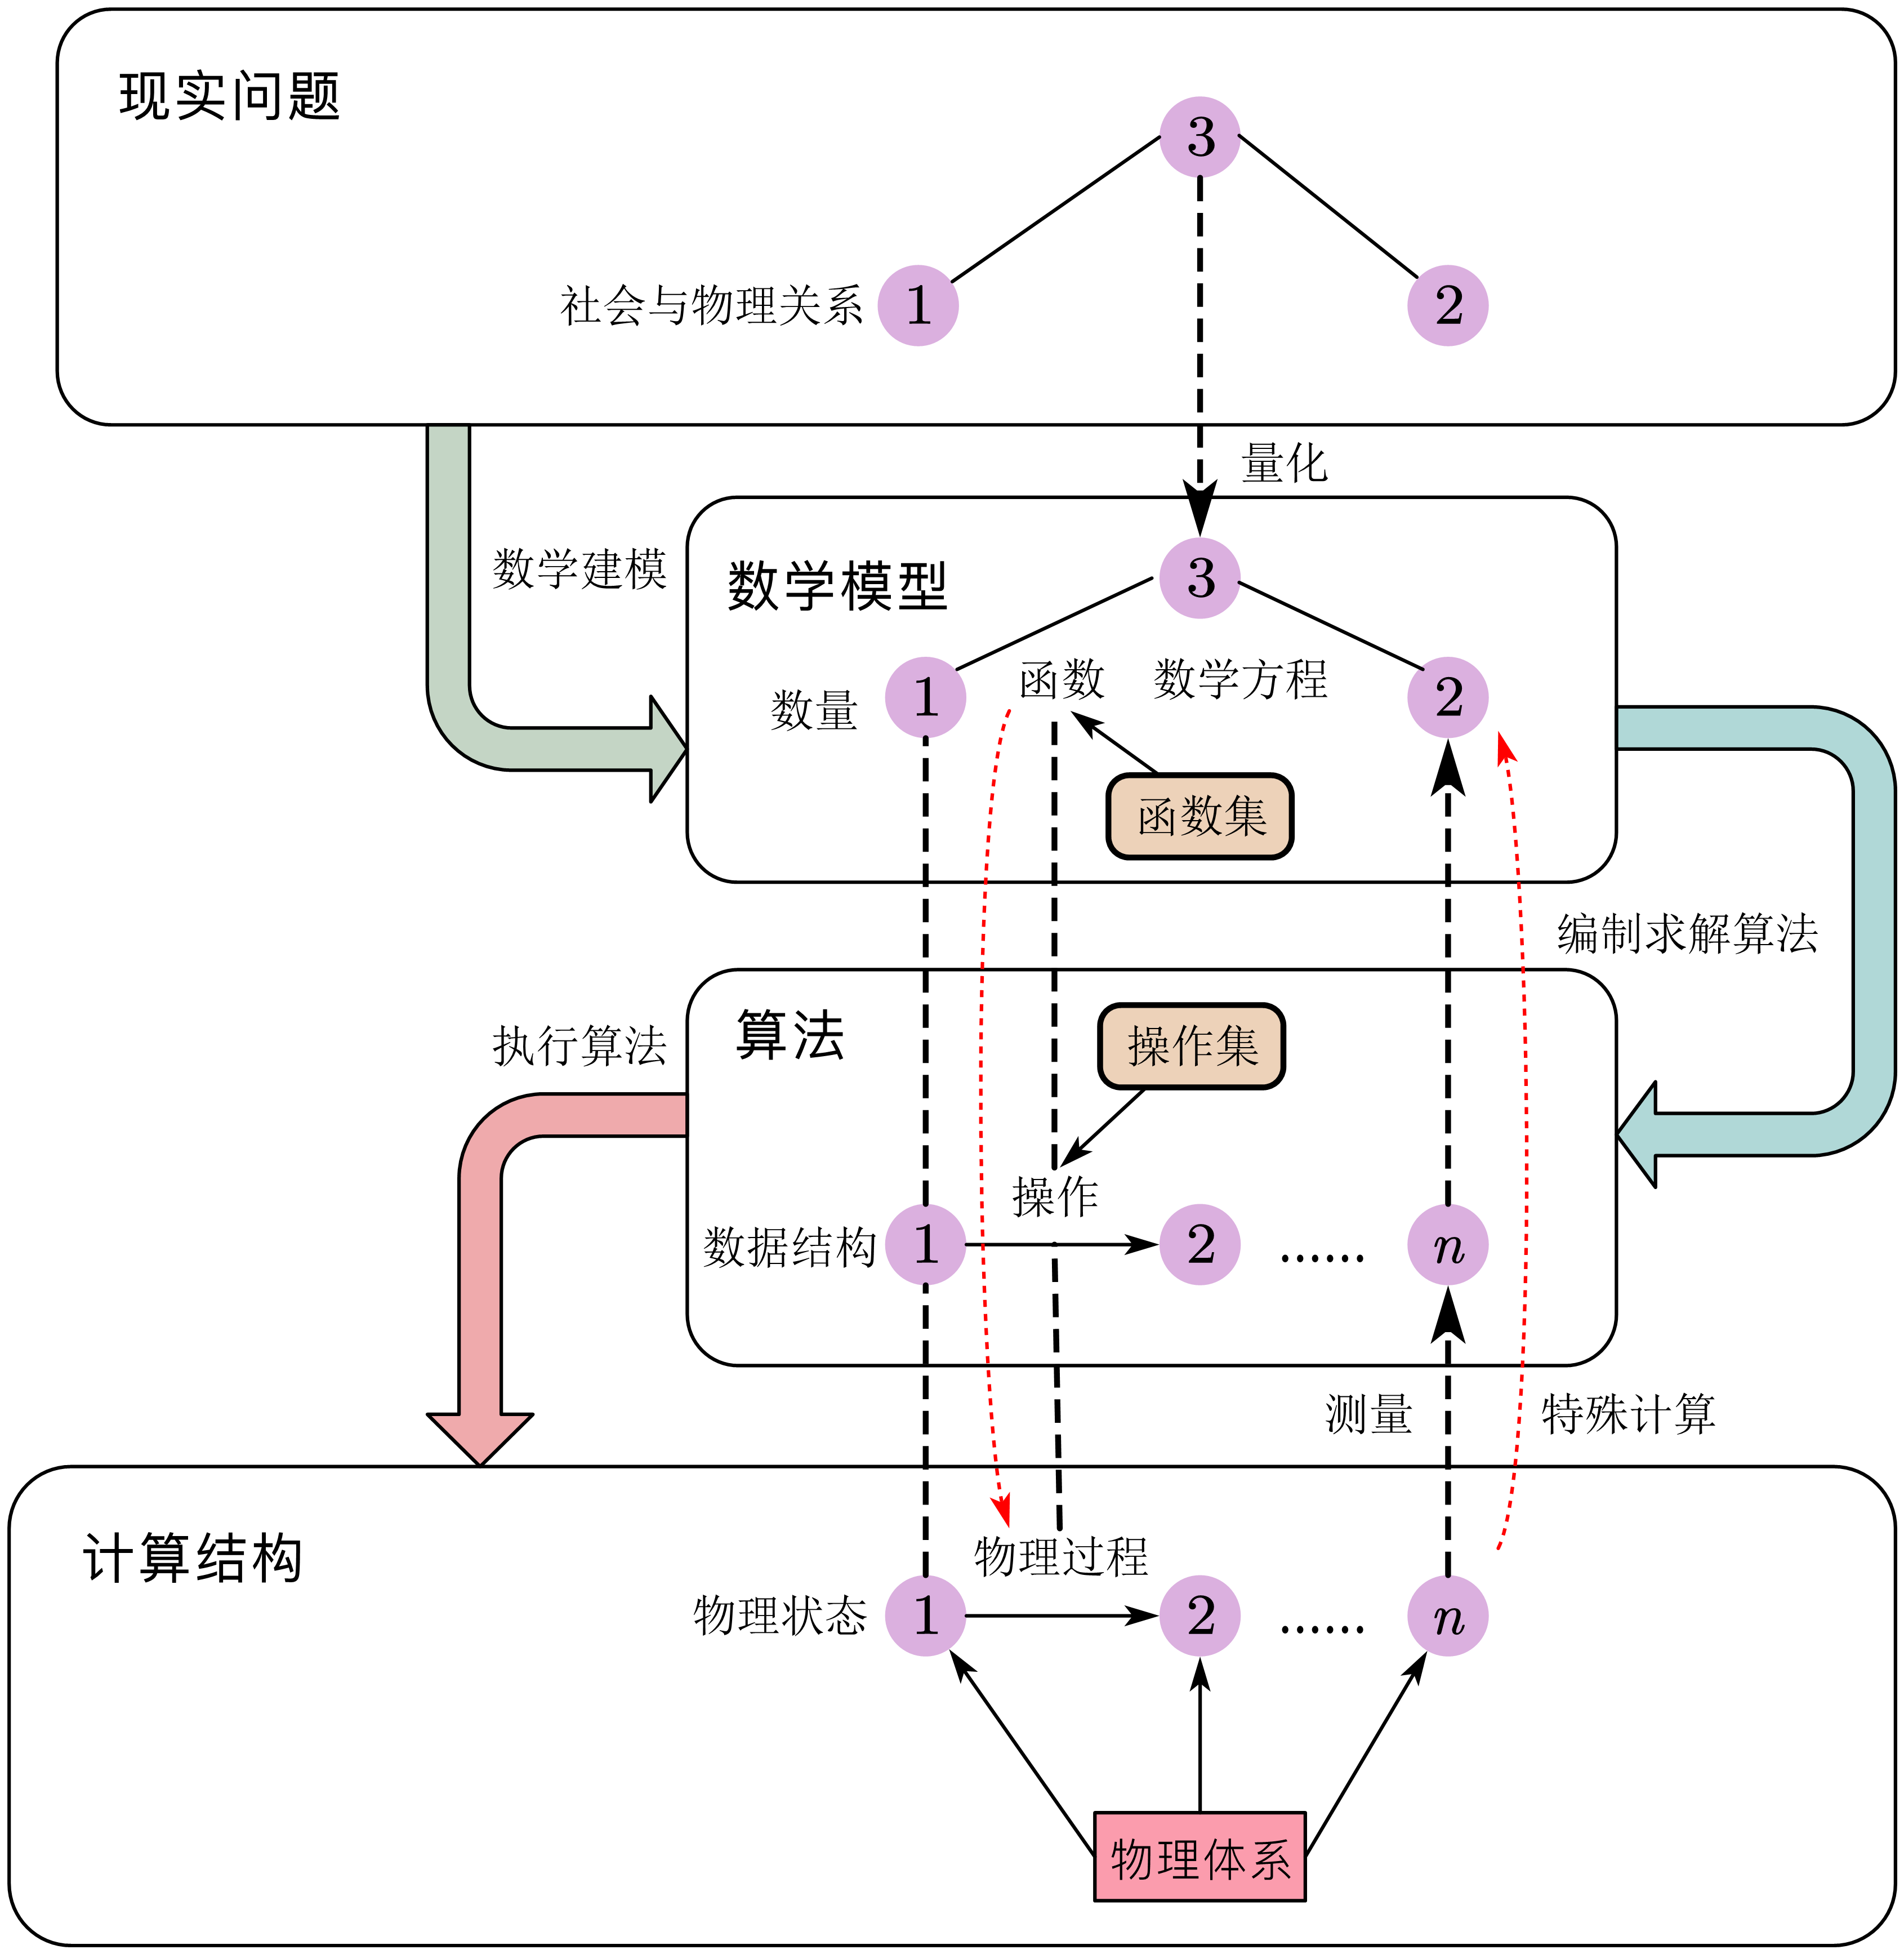
\includegraphics[width=14cm]{figure/General Computing.png}
\end{center}

图中画红线的是特殊计算,比如光子计算、蛋白质计算、神经计算等等,以区别于传统的诸如使用计算机编程的计算。


\section{量子计算}


\part{证明的方法}
\chapter{证明问题的常见思路}
\section{通用思路}
第一,尝试对原问题进行转换.

第二,证明逆否命题.

第三,构造法:构造反例、正例.

第四,从部分到整体.

阅读证明时,也要从以上入手.

\section{证明存在性与不存在性}
存在性通常是指:存在某个对象,满足某种性质.证明存在性,只要能构造一个正例即可.证明不存在性,构造反例,或者假设存在,推出矛盾.

阅读已有的证明时,也要从以下入手:\circled{1}正例是什么,反例是什么;\circled{2}构造例子的过程;\circled{3}背后的直觉.

一些特殊的技巧:

\begin{enumerate}
\item 证明存在性,首先构造一类对象,部分地满足性质,再从这一类对象中选择一些特殊的对象,比如最大、最小,证明这些特殊对象恰好可以满足全部性质.在证明Hann-Banach定理\ref{hann-banach}时应用了这种思路,此处,“部分满足”是指函数的定义域非全集.从中选择极大元,它的定义域恰好是全集.

如果选择极大元,必然要求极大在元存在,有时需要Zorn引理.

这种思路基本上是从部分到整体的思路,类似地,我们可以分别构造不同类的对象,它们分别部分地满足不同的性质,再把这些对象合成一类,比如分段线性函数.

\end{enumerate}
\section{证明解集的完备性}

对于一个问题,求出了一组解,并不代表解是完备的,该问题可能存在其它解,需要证明求出的解就是原问题的解.

首先,最直观地从个数上,思路是证明\circled{1}原问题的解最多只有$n$个,\circled{2}已经求出了$n$个解.所以求出的解是完备的.

更抽象地看,“个数”是集合的一种性质,那么也可以从其它性质入手.\circled{1}原问题的解必然满足某种性质,\circled{2}满足某种性质的解只能是求出的解.所以解集是完备的.

\section{证明唯一性}
唯一性是很重要的性质,尤其是在数值计算中.

第一,可以假设存在两个不同的元素,证明这两个元素是相同的,比如差为0.

第二,在分析学中,对于迭代给出的算法,有时可以证明,假设存在一个真实的值,从任意一个初始值出发,会收敛到相同的真实值;或者对于任意不同的初始值,分别迭代后,会趋于同一个值.

\section{扩张与数学归纳法}
对于少数事物间的联系与性质,将它推广到更多的事物。通常与数学归纳法密切相关。

\chapter{证明不等式}
\section{导数法}
构造一个函数,再求导得到单调性,是一种基本思路.

有时对于一些代数函数,我们设想可以用泰勒展开,比较最高次项的符号,这样可以得到在展开点附近的导数符号.但是它不能说明整个区间上的符号.所以另一方式就是求高阶导数.这两种方式基本上是一样的,比如两个函数,如果泰勒展开相减后消去了一阶项,只有二阶.那么求二阶导再相减后,一阶项也被消去了.

\chapter{函数估计理论}
此估计非统计学中的参数估计,而是估计函数值的上下界一类的问题.

\section{常微分方程估计}
\subsection{将函数值表示为导数}
\begin{example}
	$f(1)=1$,且$\forall x\geq 1, f'(x)=\frac{1}{x^2+f^2(x)}$,试估计函数在无穷大时的取值.
\end{example}

\begin{solution}
	可以看出$f$是递增的,且$f(x)\geq 1$,那么$f'(x)\leq \frac{1}{1+x^2}$,同时$f(x)=1+\int_{1}^{x}f'(t)\dif t$,据此很容易算出来.
\end{solution}


\part{数学物理}
\chapter{物理学图景}
\section{物理学基本思想}
\subsection{最小作用量原理}

\subsection{守恒律}

\subsection{对称性}

\subsection{近似}

\section{物理学基本定义}
\subsection{物理量的单位}
\subsubsection{国际单位制}
\paragraph*{基本定义}
共有7个国际基本单位,其它单位可以从基本单位导出:

\begin{longtable}{ccc}
	\toprule
	含义 &   英文名   &      单位       \\ 
	\midrule
	时间 &         &    \si{\s}    \\
	长度 &         &    \si{\m}    \\
	质量 &         &   \si{\kg}    \\
	电流 &         &    \si{\A}    \\
	温度 & kelvin  &    \si{\K}    \\
	数量 &  mole   &   \si{\mol}   \\
	光强 luminous intensity& candela & \si{\candela} \\ 
	\bottomrule
\end{longtable}
\paragraph*{由基本单位导出的单位}
\begin{longtable}{cccc}
\toprule
名称 & 含义 &   英文名   &      单位       \\ 
\midrule
功 & & & \si{\J}=\si{\N\m} \\
电压 & 移动1单位电荷所做的功恰为1\si{\J}& & \si{\V}=\si{\J\per\coulomb}\\
电阻 & & & \si{\O}=\si{\V\per\A}\\
\bottomrule
\end{longtable}

\subsubsection{自然单位制}
国际单位制下的公式写起来比较繁琐,可以用自然单位制。在自然单位制下,某些物理量被标准化为1。最常见的就是光速标准化为$1$,即以$c$为单位。以下列出一些自然单位制。

\paragraph*{普朗克单位制}\label{planck-natural-unit}
\begin{empheq}{align}
c=G=\hbar=\inv{4\pi\varepsilon_0}=k_B&=1\\
e=\sqrt{\alpha}&\approx 0.08542
\end{empheq}

\subsection{物理学常数}
\begin{longtable}{cccc}
\toprule
名称 & 含义 &   英文名    &说明  \\ 
\midrule
光速 &$c=\frac{1}{\mu_0\varepsilon_0}$ & &这里包含了三个常数。\\
万有引力常数 & $G$& &\\
玻尔兹曼常数 & $k_B$& &\\
\bottomrule
\end{longtable}

\subsection{物理量的定义}
有些物理量是定义出来的,但具体的计算可能是通过一些近似得到,不同的近似会有不同的结果。

\begin{note}
\begin{enumerate}
	\item 速度可以是矢量(velocity)或者标量(speed),作为标量的速度就是矢量的$L_2$范数。比如对于圆周运动,$\bx=[r\cos\theta,r\sin\theta]^T$,则矢量速度
$$\bm{v}=\frac{\dif \bm{x}}{\dif t}=\begin{bmatrix}
	-r\sin\theta\frac{\dif \theta}{\dif t}\\
	r\cos\theta\frac{\dif \theta}{\dif t}
\end{bmatrix}$$
取绝对值就是$v=\omega r$,$\omega$为角速度。
\end{enumerate}

\end{note}

\chapter{经典力学}

\section{空间中的运动}
\subsection{平移与旋转}
\subsubsection{公式一览}\label{move-rot-formulas}
下表中的内容大部分来自于\cite{BibEntry2021Nov}。
\begin{longtable}{m{0.1\textwidth} m{0.38\textwidth}|m{0.1\textwidth} m{0.38\textwidth}}
\toprule
\multicolumn{2}{c|}{刚体平动} & \multicolumn{2}{c}{定轴转动} \\
\midrule
速度 &$\bm{v}=\odv{\bm{r}}{t}$  & 角速度&  $\bm{\omega}=\odv{\btheta}{t}$\\
加速度 &$\bm{a}=\odv{\bm{v}}{t}$ & 角加速度& $\balpha=\odv{\bm{\omega}}{t}$\\
 力& $\bm{F}$ & 力矩& $\bm{M}$\\
质量 & $m$ & 转动惯量& $J=\int r^2\dif m=\int r^2\rho\dif V$\\
 动量& $\bm{p}=m\bm{v}$ &角动量 & $\bm{L}=\bm{r}\times \bm{p}=J\bm{\omega}$ \\
 \midrule
 运动定律& $\bm{F}=m\bm{a}$& 转动定律& $\bm{M}=J\balpha$\\
 动量定理 & $\int_{t_0}^{t_1}\bm{F}\dif t=m(\bm{v}_1-\bm{v}_2)$& 角动量定理&$\int_{t_0}^{t_1}\bm{M}\dif t=\bm{L}_1-\bm{L}_0$\\
 动量守恒& $\sum F_i=0\iff \sum m_i\bm{v}_i=0$&角动量守恒& $\bm{M}=0\iff \sum J_i\bm{\omega}_i=\text{const}$\\
 力的功&$W=\int_{\bm{a}}^{\bm{b}}\bm{F}\cdot \dif \bm{r}$&力矩的功& $W=\int_{\btheta_0}^{\btheta_1}M\dif \theta$\\
 功率& $P=\odv{W}{t}=\frac{1}{t_1-t_0}\int_{t_0}^{t_1}F\cdot \bm{v}\dif t$&力矩的功率 & $P=\frac{1}{t_1-t_0}\int_{t_0}^{t_1}M\cdot \bm{\omega}\dif t$\\
 \midrule
 动能& $E_k=\inv{2}mv^2$& 转动动能& $E_k=\inv{2}J\omega^2$\\
 动能定理&$W=\inv{2}m(v_1^2-v_0^2)$&动能定理& $W=\inv{2}J(\omega_1^2-\omega_0^2)$\\
 重力势能&$E_p=mgh$ &重力势能 & $E_p=mgh_C$\\
 机械能守恒& 只有保守力做功$\implies E_k+E_p=\text{Const}$&同左& 同左\\ 
 \bottomrule
\end{longtable}
上式中有些量可以是矢量也可以是标量,比如$F=ma$,$F,a$即可以是矢量,也可以是标量。其实标量式就相当于矢量式取绝对值:$$F=|\bm{F}|=|m\bm{a}|=m|a|=ma$$
动量式也类似,可以取矢量或者标量。

下图为示意图:
\begin{center}
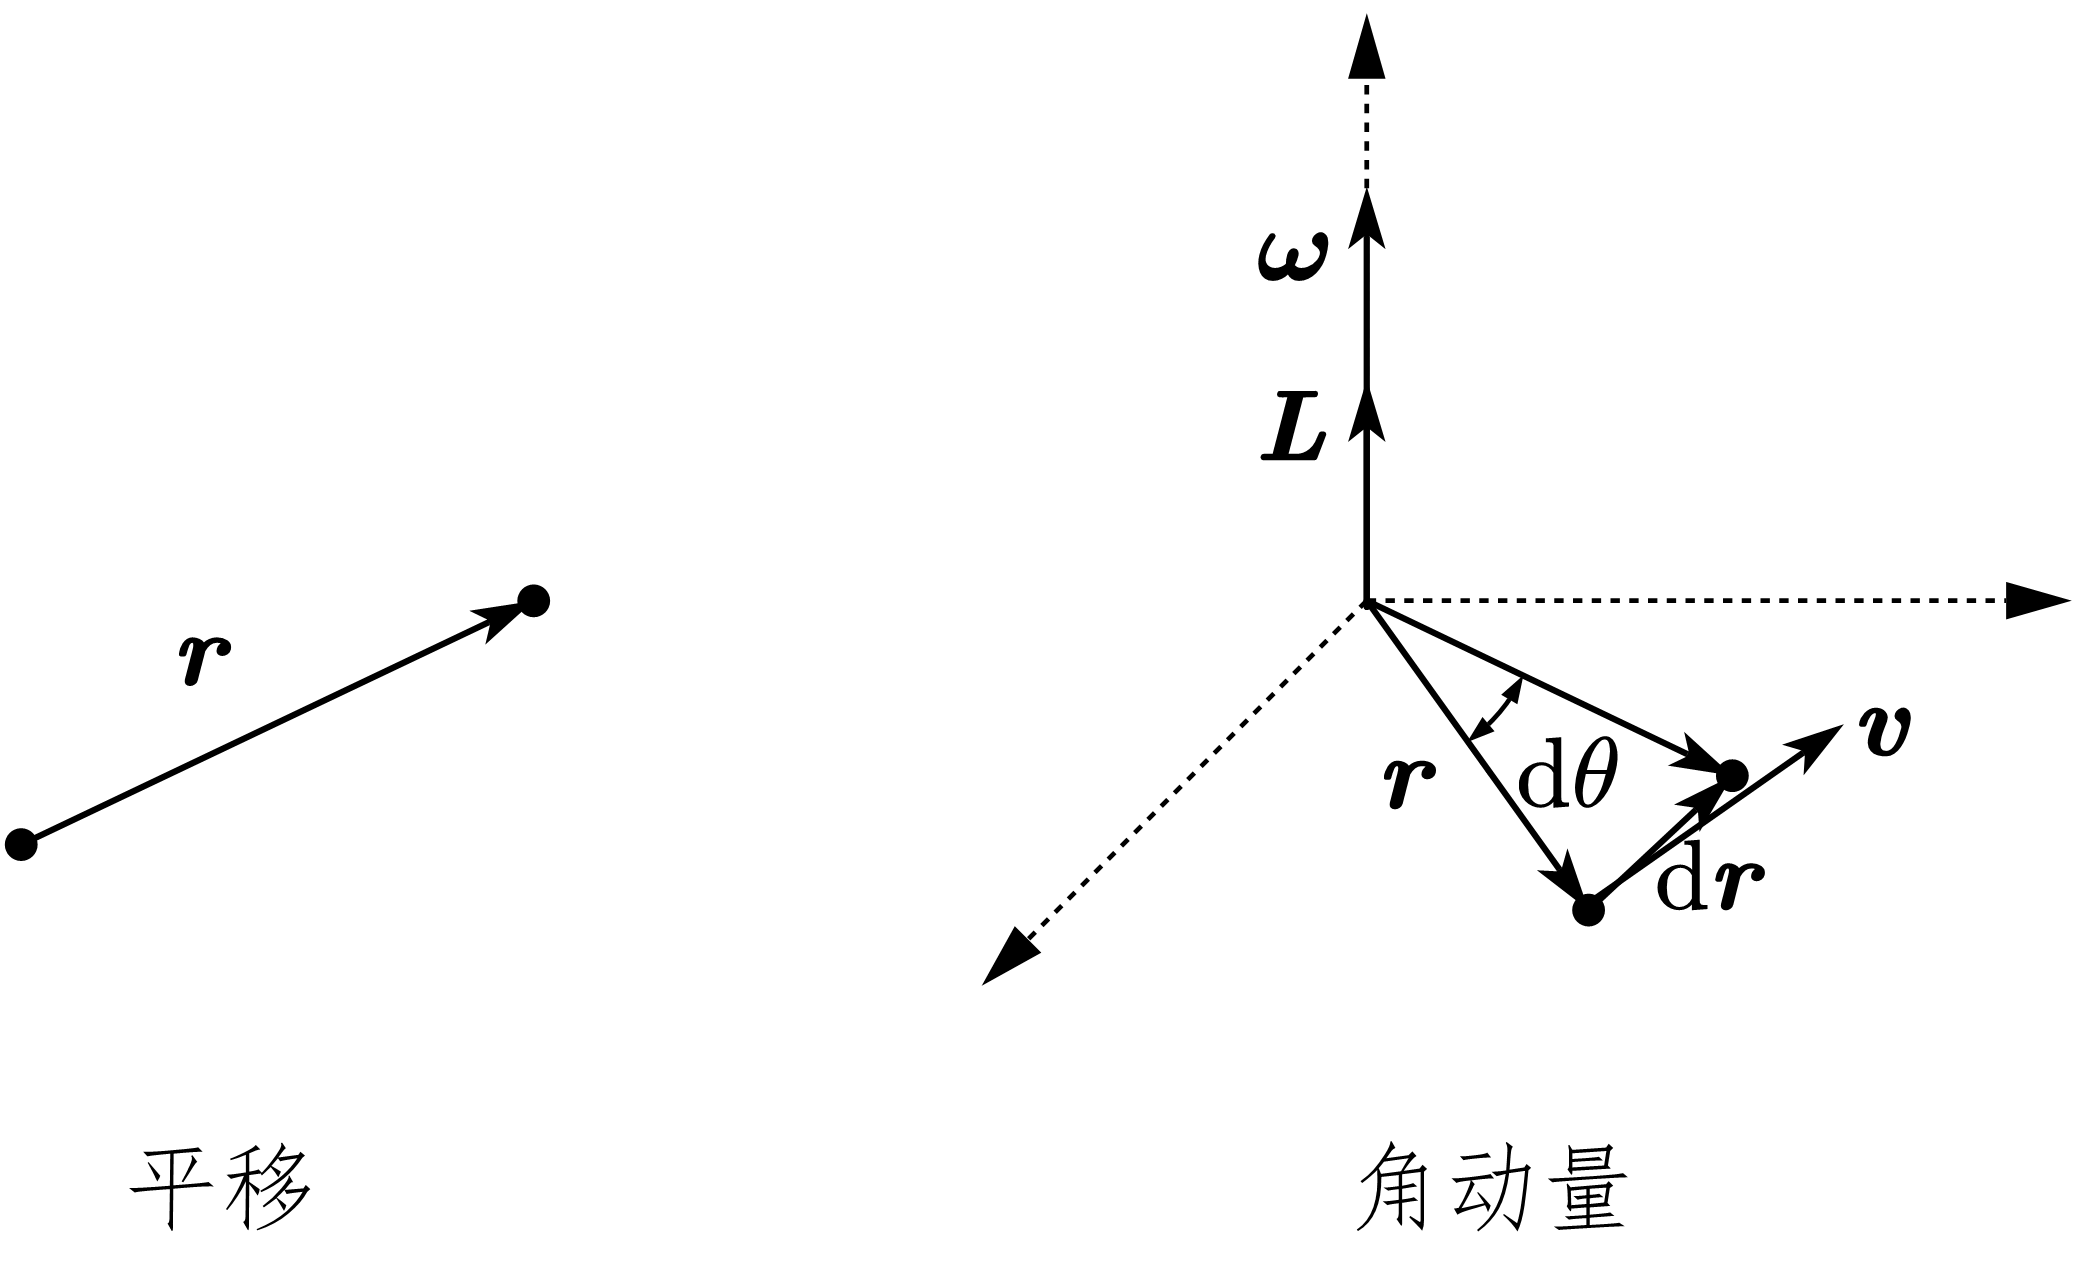
\includegraphics[width=6cm]{figure/move-in-space.png}
\end{center}

\subsubsection{抛体运动}
如下图所示,考虑炮弹的运动轨迹。

\begin{center}
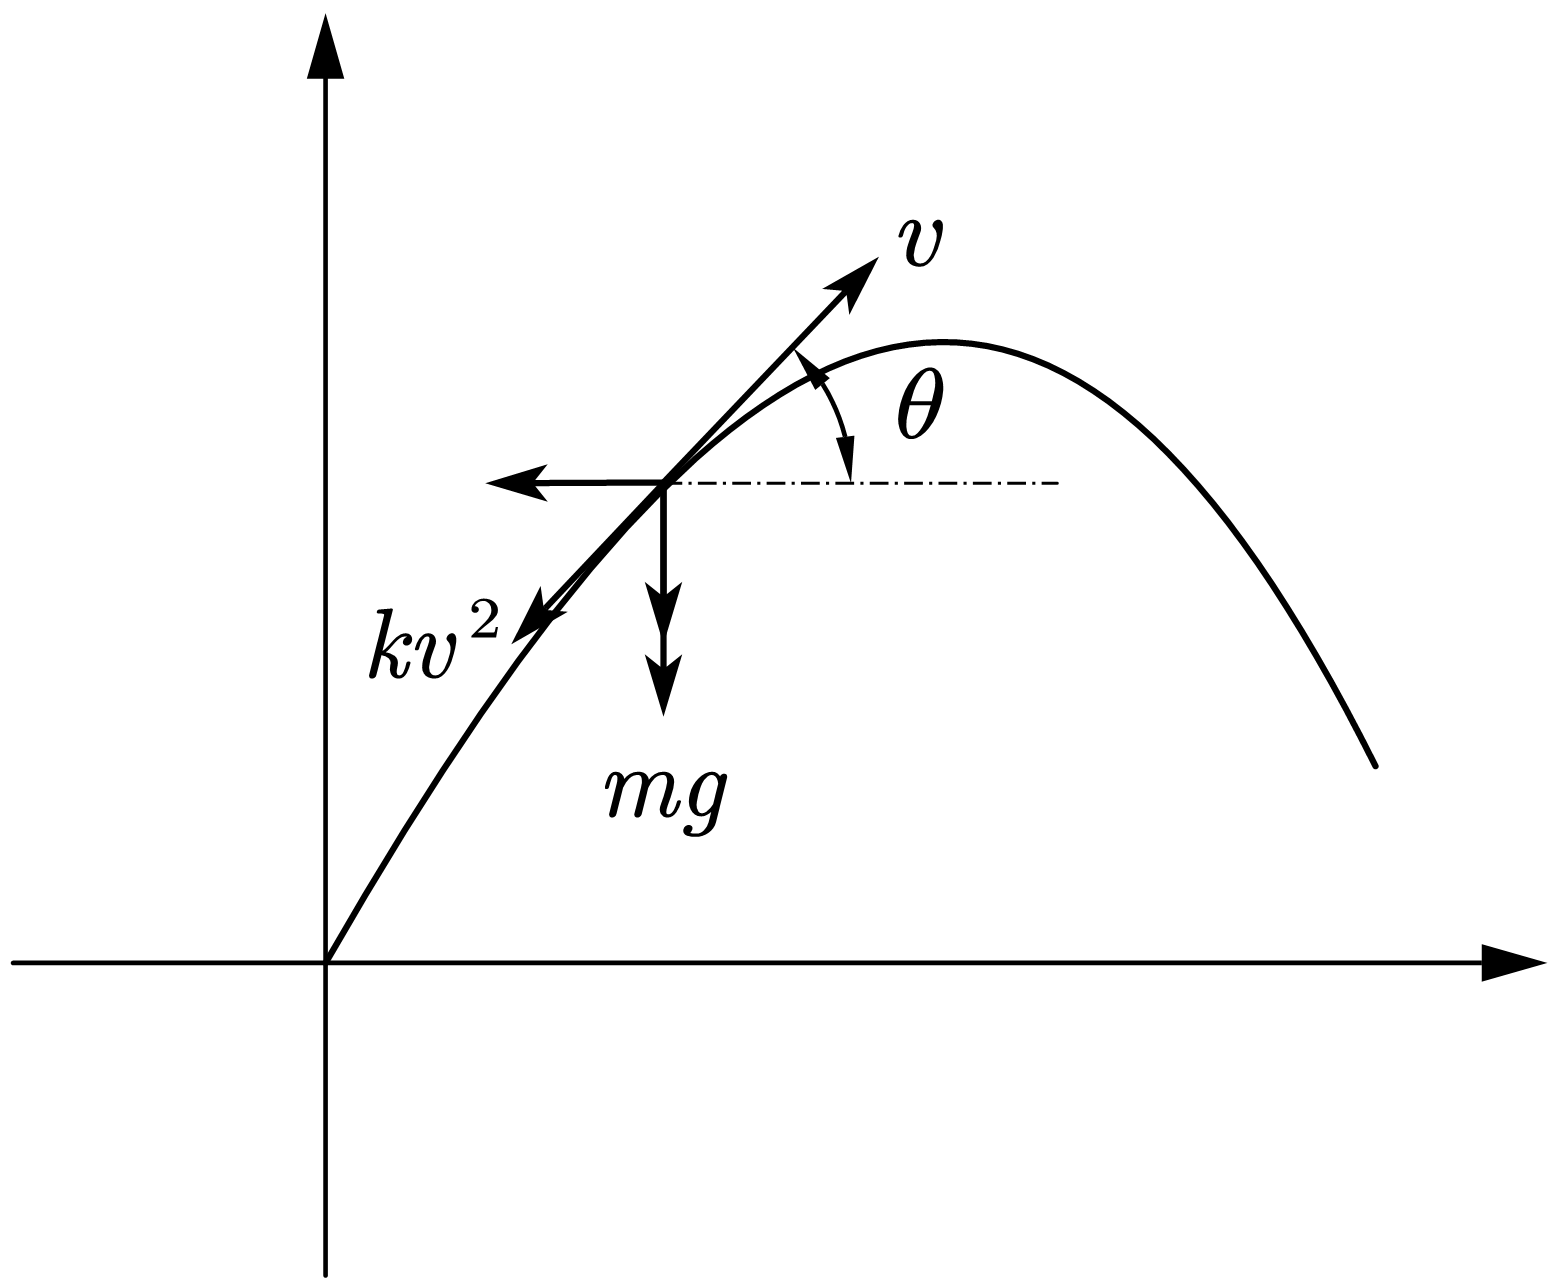
\includegraphics[width=6cm]{figure/projectile.png}
\end{center}

$f=kv^2$为阻力。$v$为速率。首先有速度方程:
\begin{empheq}{align}
\dot{x}&=v\cos\theta\\
\dot{y}&=v\sin\theta
\end{empheq}
然后有加速度方程:
\begin{empheq}{align}
\ddot{x}&=\odv{v\cos\theta}{t}=\dot{v}\cos\theta-\dot{\theta}v\sin\theta=-kv^2\cos\theta/m\\
\ddot{y}&=\odv{v\sin\theta}{t}=\dot{v}\sin\theta+\dot{\theta}v\cos\theta=-kv^2\sin\theta/m-g
\end{empheq}
这两个方程可以解出$\dot{v},\dot{\theta}$,最后得到4个方程:
\begin{empheq}[left=\empheqlbrace]{align}
\dot{v}&=-g\sin\theta-kv^2/m\\
\dot{\theta}&=-g\cos\theta/v\\
\dot{x}&=v\cos\theta\\
\dot{y}&=v\sin\theta\\
x(0)&=y(0)=0,v(0)=v_0,\theta(0)=\theta_0
\end{empheq}
实际上只有前2个方程是独立的。


\subsection{形变}

\subsection{碰撞}

\subsection{振动}

\section{拉格朗日力学}
\subsection{最小作用量原理与拉格朗日函数}
\subsubsection{最小作用量原理}


\subsubsection{拉格朗日函数的性质}
\paragraph*{可缩放}

\paragraph*{可加性}

\paragraph*{拉格朗日函数不唯一}

\paragraph*{惯性参考系}

\paragraph*{伽里略相对性原理}
\subsubsection{守恒律}
守恒律是拉格朗日函数的特殊性质。

\paragraph*{能量守恒}

\paragraph*{动量守恒}

\paragraph*{角动量守恒}

\subsection{各种情形下的拉格朗日函数}
\subsubsection{势场中的质点系}


\section{哈密顿力学}


\chapter{相对论}
\section{原理}
\subsection{洛伦兹变换}
\begin{definition}[洛伦兹变换]
假设两个坐标轴相互平等,坐标系$S'$相对另一个坐标系$S$沿$x$轴以匀速$v$运动。$(x',y',z',t'),(x,y,z,t)$分别为同一个事件在两个坐标系中的四维时空坐标,则坐标之间的变换为:
\begin{empheq}{equation}
x'=\gamma(x-vt),y'=y,z'=z,t'=\gamma(t-vx/c^2)
\end{empheq}
其中$\gamma=\inv{\sqrt{1-\beta^2}},\beta=v/c$。
\end{definition}
现在来验证它确实保持事件的间隔在两个坐标系中相同。假设第一个坐标系中发生的2个事件为$(x_1,y_1,z_1,t_1),(x_2,y_2,z_2,t_2)$,其事件间隔为
$$\Delta  s=\sqrt{c^2(t_2-t_1)^2-((x_2-x_1)^2+(y_2-y_1)^2+(z_2-z_1)^2)}$$

在第二个坐标系,对应的两个事件为$(x_1',y_1',z_1',t_1'),(x_2',y_2',z_2',t_2')$,希望验证$\Delta s'=\Delta s$。由于$x,y$坐标没有变,因此只需要验证
\begin{empheq}{equation}
c(t_2-t_1)^2-(x_2-x_1)^2=c(t_2'-t_1')^2-(x_2'-x_1')^2
\end{empheq}

对于上式
\begin{empheq}{align*}
\text{右边}&=c^2\gamma^2(t_2-t_1-v/c^2(x_2-x_1))^2-\gamma^2(x_2-x_1-v(t_2-t_1))^2\\
&=(c^2+v^2)\gamma^2(t_2-t_1)^2-v^2\gamma^2(x_2-x_1)^2\\
&=c(t_2-t_1)^2-(x_2-x_1)^2\\
&=\text{左边}
\end{empheq}
验证完成。

\subsection{时间膨胀与洛伦兹收缩}
在$S$坐标系中的同一空间坐标(固定空间),测得时间间隔为$T=t_2-t_1$,则在另一个坐标系中测得时间间隔为。

在某个坐标系中某个特定时间点(固定时间),测得物体在$x$方向的长度为$L=x_2-x_1$,则在另一个坐标系中,测得的长度为$L'=\gamma(x_2-x_1)=\gamma L$,即长度发生了收缩,这就是洛伦兹收缩。

\section{相对论力学}

\section{狭义相对论}

\section{广义相对论}

\chapter{电磁学与电动力学}
本章是以Maxwell方程组为核心来组织的。

\section{基本物理量与概念}
\subsection{电}
\subsubsection{电荷}
\paragraph*{物理对象}如下图所示为一些基本对象:
\begin{center}
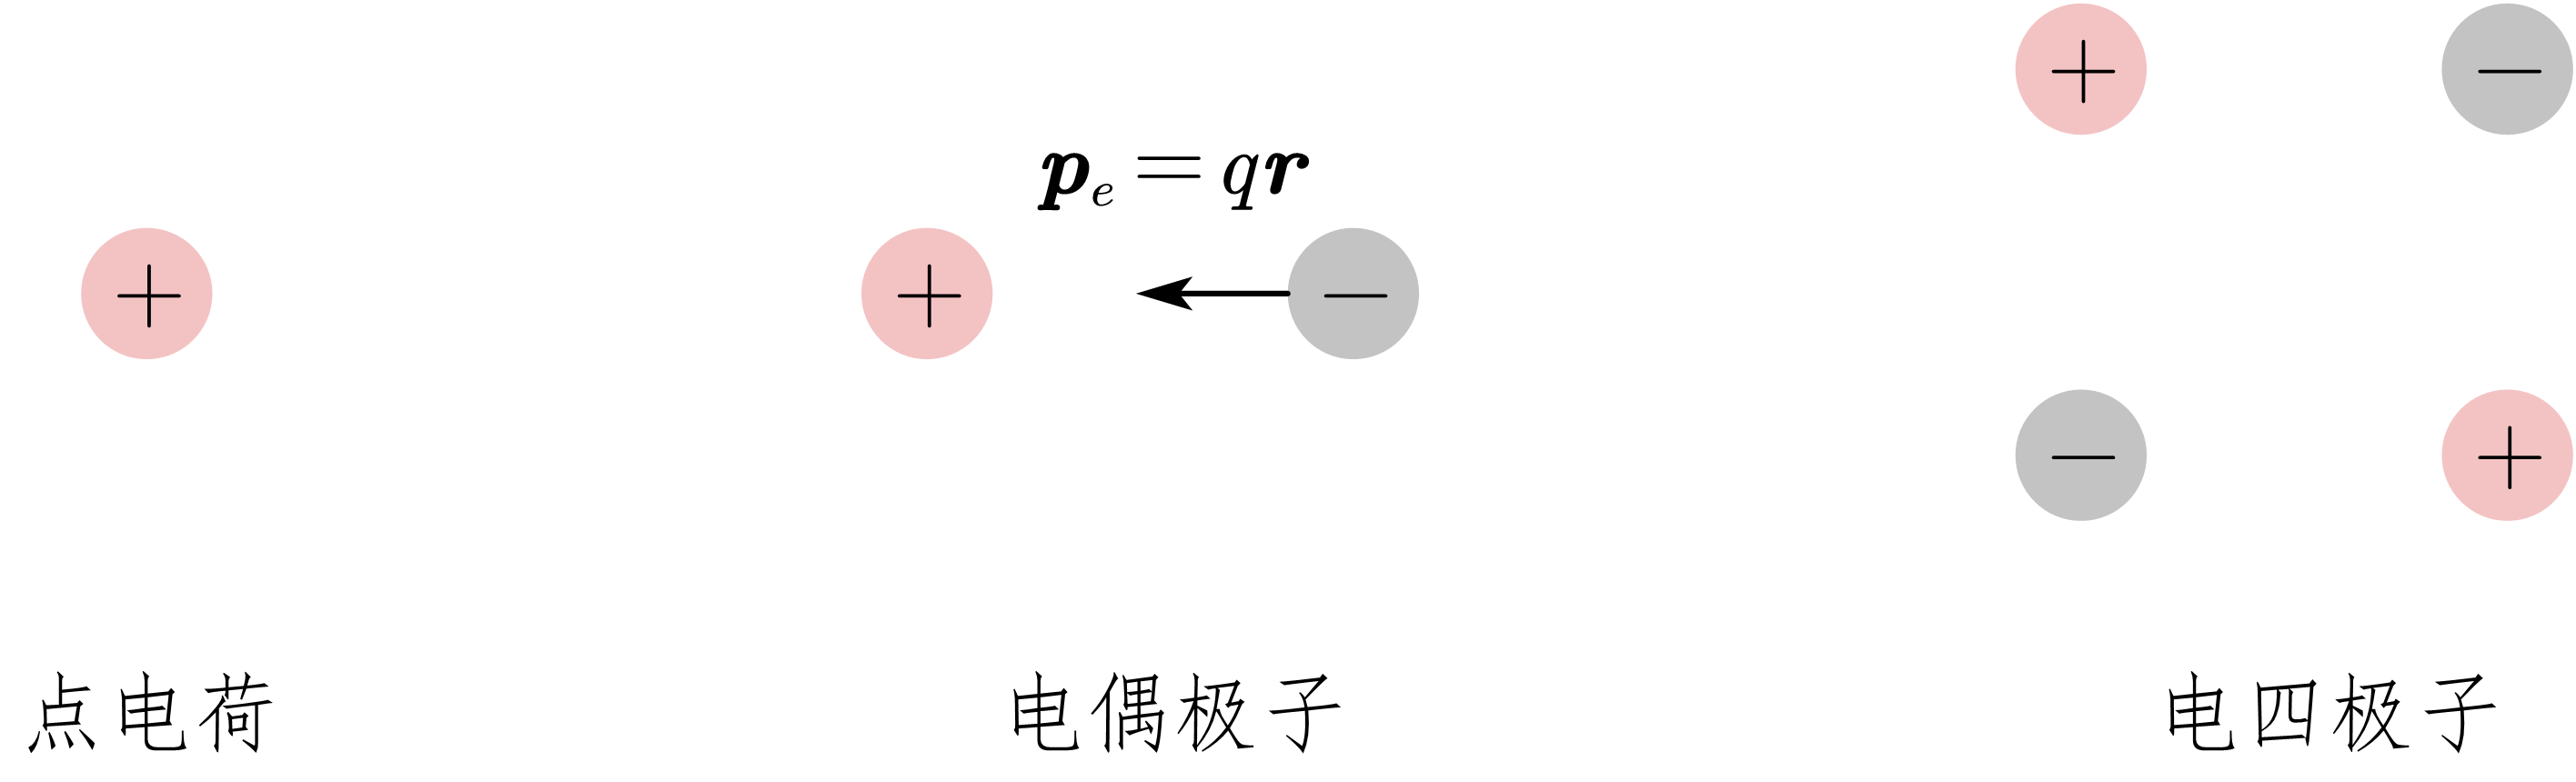
\includegraphics[width=10cm]{figure/ele-dyna-elec.png}
\label{charge-illustration}
\end{center}
\paragraph*{物理量}
\begin{description}
\item[电荷] 电荷$q$是基本粒子的基本属性.它是量子化的,即一个带电体的电荷是基本电荷电量的\qty{1.60217733e-19}{\coulomb}.夸克具有分数电荷$\pm\frac{1}{e},\pm\frac{2}{3}e$,但仍是量子化的。
\item[电荷体密度] 电荷分布在带电体上的密度,单位\si{\coulomb\per\cubic\m}:
\begin{empheq}{equation}
\rho=\odv{q}{v}
\end{empheq}
\item[电荷面密度] 电荷分布在曲面上的密度,单位\si{\coulomb\per\square\m}:
\begin{empheq}{equation}
\rho=\odv{q}{s}
\end{empheq}
\item[真空电容率] 国际单位制下为$q$\,\si{\ampere}电流在\qty{1}{\s}内累积的电荷量,也叫真空介电常数。表示为
$$\varepsilon_0=\SI{8.85e-12}{\square\coulomb\per(\newton\square\m)}$$
有时记$k=\inv{4\pi\varepsilon_0}$。
或者\si{\N\m}。
\item[偶极矩] 即之前图中的$\bm{p}_e$,一个电偶极子由偶极矩表示。
\end{description}
\subsubsection{电场}
\paragraph*{电场强度} 是一个矢量,表示为$\bE$。其大小的含义是单位正电荷在该点处所受的电场力的大小,其方向就是受力的方向。单位为\si{N\per\coulomb}。

与电场强度相关的概念有:
\begin{description}
\item[电通量] 是电场强度的曲面积分,标量:
$$\Phi_e=\iint_S \bE\cdot\dif s$$
其中$\dif s$为面片的单位元。
\item[电位移矢量] 用符号$\bm{D}$表示:
$$\bm{D}=\varepsilon_0\bm{E}+\bm{P}$$
单位\si{\coulomb\per\square\m}。对于线性各向同性的介质,有$\bm{D}=\varepsilon \bm{E}$,$\varepsilon$为电介质的绝对介电常数。电位移矢量的导数有以下表达式:
$$\pdv{\bm{D}}{t}=\nabla\times \bm{H}-\bm{J}$$
对应Maxwell方程\ref{maxwell-4}。
\item[电位移通量] 电位移矢量的曲面积分,是标量:
$$\Phi_{\bm{D}}=\iint_S\bm{D}\cdot\dif s$$ 
\item[点电荷的电场强度] 值为$\bE=k\frac{q}{r^3}\bm{r}$。它取绝对值就是$k\frac{q}{r^2}$,但是注意矢量可以叠加,但取绝对值之后不可叠加。
\end{description}
\paragraph*{电势}电场的基本属性,属于标量。含义是在某点$\bm{p}$移动1单位正电荷到零电势点$\bm{p}_0$时电场力做的功:
$$U(\bm{p})=\frac{W}{q}=\int_{\bm{p}}^{\bm{p}_0}\bE\cdot\dif \bm{l}$$
$\bm{l}$为积分路径。当电荷分布在有限区域内时,通常选择无穷远点为零电势点,则积分上界为$\infty$。电势在有的地方也用$\varphi$表示,$U$在电路中经常用来表示电压,即电势的差值。

对于静电场,电势与电场强度的关系为:
$$\bE=-\nabla U$$
由于$\vdiv \bE=0$,因此可以得到电势的拉普拉斯方程:
$$\Delta \varphi=0$$

由电势衍生出以下一些概念:
\begin{description}
\item[电势能] 电荷与电场的相互作用能。移动$q$电荷到零势能点所做的功:
$$W(\bm{p})=\int_{\bm{p}}^{\bm{p}_0}q\bE\cdot\dif \bm{l}$$
\item[点电荷的电势] 点电荷生成的电势为$U=\inv{4\pi\varepsilon_0}\frac{q}{r}$。
\item[偶极矩] 给定一个电荷体系,任取其中一个电荷为原点,则每个电荷具有径矢$\bm{r}_a$,现在考虑一个径矢为$\bm{R}_0$的点,则它的电势为:
$$\varphi=\sum \frac{q_i}{|\bm{R}_0-\bm{r}_i|}$$
这里省略系数$\inv{4\pi\varepsilon_0}$。如下图所示:
\begin{center}
\includegraphics[width=4cm]{figure/elec-mag-single-point-charge-u.png}
\end{center}

当$\bm{R}_0\gg \bm{r}_i$时,把势函数在$\bm{R}_0$处展开:
\begin{empheq}{align}
\varphi=\frac{\sum q_i}{R_0}-\sum e_i \bm{r}_i\cdot \nabla \inv{R_0}
\end{empheq}
以上结论是通过取$f(\bx)=\sum \frac{q_i}{|\bx|}$,对它用一阶近似得到的。于是取
$$\bm{d}=\sum q_i\bm{r}_i$$
为电荷体系的偶极矩。

当$\sum q_i=0$时,偶极矩与坐标无关。同时,有该电荷体系在远距离处的电势为:
$$\phi=-\bm{d}\cdot\nabla\frac{1}{R_0}=\frac{\bm{d}\cdot \bm{R}_0}{R_0^3}$$
电场强度为
$$\bE=-\nabla \frac{\bm{d}\cdot\bm{R}_0}{R_0^3}=-\inv{R_0^3}\nabla (\bm{d}\cdot\bm{R}_0)-(\bm{d}\cdot\bm{R}_0)\nabla \inv{R_0^3}$$


对于图\ref{charge-illustration}中的电偶极子,偶极矩就是$\bm{d}=q\bm{r}$,取绝对值$d=qr$,这时与一般的定义一致。这里$\bm{r}$是从负电荷指向正电荷的径矢。
\end{description}

\subsubsection{电介质}
\paragraph*{带电荷导体的静电场}一个带电荷导体具有静电场,在静电平衡时,其内部的场强必然为0,否则引起电荷运动。因此平衡时电荷应该分布在导体的表面,且导体表面的电场强度应该垂直于表面,或切向分量为0:
$$\bE_t=\bm{0}$$
否则引起电荷在切向的运动。由于$\bE=-\nabla \varphi$,因此导体在表面的电势应当相同。

根据$\vdiv \bE=4\pi\bar{\rho}$,$\bar{\rho}$为平均电荷密度。可得$E_{\bn}=4\pi\sigma$,$\sigma$为电荷的面密度。然后有:
\begin{empheq}{align}
\sigma&=\inv{4\pi}E_n=-\inv{4\pi}\pdv{\varphi}{n}\mtag{导体表面的电荷分布}\\
e&=-\inv{4\pi}\oint \pdv{\varphi}{n}\dif s \mtag{导体表面的总电荷}
\end{empheq}
总电荷就是对面密度积分。

\paragraph*{带电荷导体的静电场能量}系统的总能量为:
\begin{empheq}{equation}
\mathcal{U}=\inv{8\pi}\int\bE^2\dif V=\inv{2}\sum_a e_a\varphi_a
\end{empheq}
\paragraph*{带电荷导体的电容}电势与电荷的关系应该为线性的,这是因为场的叠加特性,于是有
\begin{empheq}{equation}
e_a=\sum_b C_{ab}\varphi_b
\end{empheq}
$C_{aa}$称为\emph{电容系数},$C_{ab}(a\neq b)$称为\emph{静电感应系数},它们与导体的特性有关。如果只有一个导体$e=C\varphi$,$C$就是一般的电容。

相应地
\begin{empheq}{equation}
\varphi_a=\sum_b C_{ab}^{-1}e_b
\end{empheq}
注意$C_{ab}^{-1}$为逆矩阵的系数,不是$\inv{C_{ab}}$。



\paragraph*{电导率} 表示为$\sigma$,刻画导体中电荷流动的难易程度:
$$\bm{j}=\sigma \bE$$
$\bm{j}$是电流密度。
\paragraph*{极化}电介质在外电场中时,在电场的作用下,电介质内部或者表面出现净束缚电荷(极化电荷),这此电荷产生附加电场,从而改变了原来的电场分布,就叫极化。以下为一些描述极化的量:
\begin{description}
\item[电极化强度] 用$\bm{P}$表示,等于单位体积内电偶极矩的矢量和:
\begin{empheq}{equation}
\bm{P}=\frac{\sum \bm{p}_{分子}}{\Delta V}
\end{empheq}
单位为\si{\coulomb\per\square\m}。
\item[极化率] 极化强度对电场强度的比值$\chi_{\varepsilon_0}$:
$$\bm{P}=\chi_{\varepsilon_0}\bE$$
\item[介电常数] 又称为电容率:
\begin{empheq}{align}
\varepsilon&=\varepsilon_0\varepsilon_r\\
\varepsilon_r&=1+\chi_{\varepsilon_0}
\end{empheq}
$\varepsilon$为绝对介电常数,$\varepsilon_r$为相对介电常数。
\end{description}
\subsubsection{直流电}
电流就是电荷的运动,具体地说是单位时间内通过单位面积的电荷量。如果是金属导电流,就是电子的运动。直流电就是电荷只向同一个方向运动。

\paragraph*{电阻}电阻就是导体对电流运动的阻碍,通常记为$R\si{\ohm}$,电阻率为$\rho \si{\ohm\meter}$,电导率$\rho=\inv{1}{R}$。有以下关系式:
\begin{empheq}{align}
\rho&=\frac{RS}{l}\mtag{均匀导体}\\
\dif R=\rho(x)\frac{\dif x}{A(x)}&\implies R=\int_{a}^{b}\inv{\rho(x)A(x)}\dif x \mtag{非均匀导体}
\end{empheq}
$l$为导体长度,$S,A$为横截面积。


\paragraph*{电流密度}电流本身为标量,不是矢量。但电流密度$\bm{j}$是矢量,电流强度$I$与它的关系为:
$$I=\iint_S \bm{j}\cdot\dif \bm{S}$$
如果是均匀电流,则
$$I=jS$$
此处$j=|\bm{J}|$。
\paragraph*{平均漂移速度}飘移速度是电子的运动速度,它与电流密度的关系为
$$\bm{j}=nev\bar{v}$$
$n$为流过截面的电子个数。

\paragraph*{电压}用$U$表示,单位\si{\volt}。对于一段导线,假如它没有电阻,则各点处电压相同,不妨称为平衡原理。

\paragraph*{欧姆定律}给出了电势差、电流强度、电阻的关系:
$$U=IR$$

\paragraph*{功率}电流的功率为:
$$P=IU=I^2R=\frac{U^2}{R}$$

\paragraph*{串联与并联电路}如下图所示:
\begin{center}
\includegraphics[width=14cm]{figure/seq-vs-parrllel-circuit.png}
\end{center}

\paragraph*{基尔霍夫定律}描述复杂电路中支路的电流与电压的关系,在每个节点处有:
\begin{empheq}{align}
\sum_{k=1}^{n}i_k&=0\mtag{基尔霍夫第一定律}\\
\sum_{j=1}^{n}v_j&=0\mtag{基尔霍夫第二定律}
\end{empheq}
当电流注入节点时,$i_k$为正,否则为负。$v_j$表示某个元件的电势差(有正负)。第一定律针对节点,也可以表达为注入某节点的电流等于流出节点的电流。第二定律针对整个闭合回路(电源也算,回路也可以是电路的一部分)。

\paragraph*{惠更斯电桥}一五电阻电路:
\begin{center}
\includegraphics[width=8cm]{figure/5R-elec-bridge.png}
\end{center}
用并联与串联电路不能求解,需要使用基尔霍夫定律。
对于图示的三个回路有:
\begin{enumerate}
\item 回路1,$acda$:$I_1R_1+I_5R_5-I_3R_3=0$
\item 回路2,$acbda$:$(I_1-I_5)R_2-(I_3+I_5)R_4-I_5R_5=0$
\item 回路3,$acbUa$:$I_1R_1+(I_1-I_5)R_2-U=0$
\end{enumerate}
电流有3个,方程有3个,且为线性方程组,可以求解:
\begin{empheq}{align}
I_1&=\frac{U}{\Delta}((R_2+R_4)R_3+(R_3+R_4)R_5)\\
I_3&=\frac{U}{\Delta}((R_2+R_4)R_1+(R_1+R_2)R_5)\\
I_5&=\frac{U}{\Delta}(R_2R_3-R_1R_4)\\
\Delta &=R_1R_2(R_3+R_4)+R_3R_4(R_1+R_2)+(R_1+R_2)(R_3+R_4)R_5
\end{empheq}
可知
$$I=I_1+I_3=\frac{U}{\Delta}((R_1+R_3)(R_2+R_4)+(R_1+R_2+R_3+R_4)R_5)$$
于是$ab$间电阻为:
$$R_{ab}=\frac{U}{I}=\frac{R_1R_2(R_3+R_4)+R_3R_4(R_1+R_2)+(R_1+R_2)(R_3+R_4)R_5}{(R_1+R_3)(R_2+R_4)+(R_1+R_2+R_3+R_4)R_5}$$

\subsubsection{交流电}

\subsection{磁}
\subsubsection{磁场}
磁场可以内磁感应强度来刻画:

\paragraph*{磁感应强度Magnetic induction} 与电场强度对应,描述了磁场的大小和方程。用$\bB$表示,单位\si{\N\s\per(\coulomb\m)}=\si{\N\per(\ampere\m)},称为特斯拉,用\si{\tesla}表示。$\bB$的尤洛卡为单位正电荷以单位速度通过该点时受到的最大作用力:
$$B=\frac{F_{\max}}{qv},\quad \bm{F}=q(\bB\times\bm{v})$$

由磁感应强度衍生出:
\begin{description}
\item[磁感应通量]\label{magnetic-induction-flux} 与电通量对应:
$$\Phi_{\bB}=\iint_S\bB\cdot\dif \bm{s}$$
单位\si{\tesla\square\m},叫做韦伯,符号\si{\weber}。
\item[磁场强度] 为了方便书写而引入的符号,用$\bm{H}$表示:
$$\bm{H}=\frac{\bB}{\mu_0}-\bm{M}$$
\end{description}

\paragraph*{磁矢势}磁场是有旋无散场,即$\nabla\cdot \bB=0$,则根据向量分析的定理\ref{vec-ana-div-zero},存在$\bm{A}$,满足$\bB=\nabla \times \bm{A}$。$\bm{A}$就称为磁矢势。

\begin{description}
\item[磁矩]  考查运动电荷体系产生的磁势。记$\bar{\bA}$为平均矢势,即对时间的平均,现在它只是对坐标的函数。类似于电极矩中的定义,以$\bm{r}_i$记径矢,则磁矢势
$$\bar{\bA}=\frac{1}{c}\frac{\bar{q_i\bm{v}_i}}{|\bm{R}_0-\bm{r}_i|}$$
展开为幂级数:
$$\bar{\bA}=\inv{cR_0}\sum q\bar{\bm{v}}-\inv{c}\sum \overline{q\bm{v}\left(\bm{r}\cdot \nabla \inv{R_0}\right)}$$
对第一项
$$\sum q\bar{\bm{v}}=\overline{\odv{}{t}\sum q\bm{r}}=0$$
这是因为在一个有限范围内变化的量的导数的均值为0。还剩下一项
$$\bar{\bA}=-\inv{c}\sum \overline{q\bm{v}\left(\bm{r}\cdot \nabla \inv{R_0}\right)}=\inv{cR_0^3}\sum \overline{q\bm{v}(\bm{r}\cdot\bm{R}_0)}$$
注意到$\bm{v}=\dot{\bm{r}}$,于是
$$\sum q\bm{v}(\bm{r}\cdot\bm{R}_0)=\inv{2}\odv{}{t}\sum q\bm{r}(\bm{r}\cdot\bm{R}_0)+\inv{2}\sum q(\bm{v}(\bm{r}\cdot\bm{R}_0)-\bm{r}(\bm{v}\cdot\bm{R}_0))$$
第一项的平均也是0,则
$$\bar{\bA}=\inv{2cR_0^3}\sum\overline{q(\bm{v}(\bm{r}\cdot\bm{R}_0)-\bm{r}(\bm{v}\cdot\bm{R}_0)}$$
记
$$\bm{\mathfrak{m}}=\inv{2c}\sum q\bm{r}\times \bm{v}$$
为磁矩。此时
$$\bar{\bA}=\frac{\bar{\bm{\mathfrak{m}}}\times \bm{R}_0}{R_0^3}=\nabla \inv{R_0}\times\bar{\bm{\mathfrak{m}}}$$
这里参考$\times$的运算公式\cref{triple-cross-prod-rule}。利用磁矩可以改写磁场公式:
$$\bar{\bH}=\vcurl \bar{\bA}=\vcurl \frac{\bar{\bm{\mathfrak{m}}}\times \bm{R}_0}{R_0^3}=\bar{\bm{\mathfrak{m}}}\vdiv \frac{\bm{R}_0}{R_0^3}-(\bar{\bm{\mathfrak{m}}}\cdot\nabla)\frac{\bm{R}_0}{R_0^3}$$
由于$\vdiv \vdiv \frac{\bm{R}_0}{R_0^3}=0$,且
$$(\bar{\bm{\mathfrak{m}}}\cdot\nabla)\frac{\bm{R}_0}{R_0^3}=\frac{\bar{\bm{\mathfrak{m}}}}{R_0^3}-\frac{3\bm{R}_0(\bar{\bm{\mathfrak{m}}}\cdot\bm{R}_0)}{R_0^5}$$
因此
$$\bar{\bH}=\frac{3\bm{n}(\bar{\bm{\mathfrak{m}}}\cdot\bm{n})-\bar{\bm{\mathfrak{m}}}}{R_0^3}$$

假如电荷具有相同的荷质比,则磁矩
$$\bm{\mathfrak{m}}=\inv{2c}\sum q\bm{r}\times \bm{v}=\frac{q}{2mc}\sum m\bm{r}\times \bm{v}=\frac{q}{2mc}\sum \bm{r}\times \bm{p}=\frac{q}{2mc}\bm{M}$$
当$v\ll c$时,$\bm{p}=m\bm{v}$为动量,$\bm{M}$为角动量,参考\ref{move-rot-formulas}。即磁矩与角动量之比为常数。
\end{description}
\subsubsection{磁介质}
\paragraph*{磁导率Magnetic permeability}表征磁介质导磁性能的物理量,
\begin{empheq}{align}
\mu&=\mu_0\mu_r\\
\mu_r&=1+\chi_m
\end{empheq}
$\mu$为绝对磁导率,$\mu_0$为真空磁导率,$\mu_r$为相对磁导率。
\paragraph*{磁化}
原来不显示磁性的磁介质在外加磁场$\bB_0$的作用下显示磁性,产生附加磁场。磁化后在介质的表面或者内部会产生等效的磁化电流,磁化电流产生磁场$\bB'$,则磁介质内部的总磁场为$\bB=\bB'+\bB_0$。

描述磁化的物理量有:
\begin{description}
\item[磁化强度] 向量。描述介质磁化程度的量。用$\bm{M}$表示:
$$\bm{M}=\frac{\sum \bm{m}_{\text{分子}}}{\Delta V}$$
即单位体积内分子磁矩的的矢量和,单位\si{\ampere\per\m}。
\item[磁化率] 磁化强度$\bm{M}$与磁场强度$\bm{H}$的关系叫介质的磁化规律,比例称为磁化率,用$\chi_m$表示:
$$\bm{M}=\chi_m\bm{H}$$
\end{description}

\subsection{相互作用}
\subsubsection{受力}
\paragraph*{洛伦兹力}运动电荷在电磁场中的受力:
$$\bm{F}=q(\bE+\bm{v}\times \bB)$$
如果磁感应强度为0,或者静止,显然只受电场力。由于磁场力是垂直于运动方向的,所以磁场不做功。

\paragraph*{安培力}电流元在磁场中的受力:
$$\dif \bm{F}=I\dif\bm{l}\times\bB$$
对一段导线进行积分,可以求得整个导线在磁场中受的合力。

\paragraph*{安培定律}描述了两个电流元间的相互作用力:
$$\dif \bm{F}_{21}=\frac{\mu_0}{4\pi\varepsilon_0}\frac{I_1I_2\dif\bm{l}_2(\dif \bm{l}_1\times\bm{e}_{21})}{r_{21}^2}$$
对于两段平行导线,这个作用力是:
$$F=\frac{\mu_0}{2\pi}\frac{I_1I_2}{r^2}$$

\subsubsection{电磁感应}
\paragraph*{磁$\rightarrow$电}导体运动或者磁场变化引用的电动势。如下图所示:

\begin{center}
\includegraphics[width=6cm]{figure/magnetic-to-current.png}
\end{center}

\begin{description}
\item[感生电动势induced electromotive force] 导体不动,由磁场变化而引发的电动势:
$$\varepsilon =\oint_L\bE\cdot\dif\bm{l}=\oiint_S \pdv{\bB}{t}\cdot\dif \bm{s}$$

一个特殊的情形是法拉弟电磁感应:
$$\varepsilon=-\odv{\Phi_{\bB}}{t}$$
$\Phi_{\bB}$为磁感应通量\ref{magnetic-induction-flux}。
\end{description}


\paragraph*{电$\rightarrow$磁}
\begin{description}
\item[毕奥-萨伐尔定律Biot-Savart]给出了电流元激发的磁感应强度。而电流是电荷的运动。

$$\dif \bB=\frac{\mu_0}{4\pi\varepsilon_0}\frac{I\dif \bm{l}\times \bm{e}_r}{r^2}$$

$\dif\bm{l}$是电流元,$r$是电流元到点的距离,$\bm{e}_r$是电流元指向点的单位矢量。对上式积分可以求出任意形状曲线在某点处的磁感应强度。
\end{description}

\subsection{电磁波}

\subsection{电磁场的张量分析}
这部分内容主要来自朗道的《场论》,使用了相对论原理。

\subsubsection{四维矢量}
\paragraph*{事件坐标与四维径向矢量} 四维时空的一个事件的坐标记为:$(x^0,x^1,x^2,x^3)=(ct,x,y,z)$。该矢量长度的平方为$(x^0)^2-(x^1)^2-(x^2)^2-(x^3)^2$,它在四维坐标系的任意转动下不变。
\paragraph*{四维矢量的定义}如果四个量$A^0,A^1,A^2,A^3$在四维坐标系的变换下像四维径向矢量那样变换,就称为四维矢量$A^i$。在洛伦兹变换下:
\begin{empheq}{align}
A^0&=\frac{A^{'0}+V/cA^{'1}}{\sqrt{1-V^2/c^2}}\\
A^1&=\frac{A^{'1}+V/cA^{'0}}{\sqrt{1-V^2/c^2}}\\
A^2&=A^{'2}\\
A^3&=A^{'3}
\end{empheq}
同时引入$(A_0,A_1,A_2,A_3)=(A^0,-A^1,-A^2,-A^3)$。$A^i$称为四维矢量的逆变分量,$A_i$称为协变分量。

量$A^iB_i$为一个标量,类似地有$A^iA_i$,即四维矢量的长度平方。分量$A^0$称为四维矢量的时间分量,$A^1,A^2,A^3$称为空间分量。四维矢量的平方可以为正(类时矢量)、负(类空矢量)、零(类光矢量)。

在纯空间转动(不影响时间)下,三个空间分量构成一个三维矢量$\bm{A}$,此时也记
\begin{empheq}{align}\label{elect-mag-4d-vec-def}
A^i&=(A^0,\bm{A})\\
A_i&=(A^0,-\bm{A})\\
x^i&=(ct,\bm{r})\\
x_i&=(ct,-\bm{r})\\
x^ix_i&=c^2t^2-\bm{r}^2
\end{empheq}

\paragraph*{二阶四维张量}对应于矩阵。是16个量$A^{ik}$的集合,在坐标变换下像两个四维矢量分量的积那样变换。一个二阶张量的分量可以写成三种形式:协变的$A_{ik}$,逆变的$A^{ik}$,混合的$A^i_{\ k}$、$A_{\ i}^k$。

这些分量之间的变换规则是:
\begin{enumerate}
\item 升降一个空间指标时变号:$A_0^{\ 1}=A^{01},A^1_{\ 1}=-A^{11}=A_{11}$。则升降两个空间指标不变号:$A^{11}=A_{11}$。
\item 升降时间指标不变号:$A^0_{\ 0}=A^{00}=A_{00},A_{00}=A^{00},A_{01}=-A^{01}$。
\end{enumerate}

如果$A^{ik}=A^{ki}$,则称为对称张量。如果$A^{ik}=-A_{ki}$,则称为反对称张量,反对称张量的对角线元素为0。

\paragraph*{四维张量的运算}
\begin{description}
\item[缩并] $A^i_{\ i}=A^0_{\ 0}+A^2_{\ 2}+A^3_{\ 3}+A^4_{\ 4}$,这里$A^i_{\ i}=A^{\ i}_i$。
\item[]
\end{description}

\paragraph*{单位张量与度规张量}单位四维张量 $\delta^i_j$,其实就是$\delta$函数。对$\delta^i_j$升降指标得到度规张量$g^{ik},g_{ik}$,两个的分量相同,其矩阵式为$(g^{ik})=(g_{ik})=\diag([1,-1,-1,-1])$。度规张量与四维矢量的计算如下:
$g_{ik}A^k=A_i,g^{ik}A_k=A^i,A^iA_i=g_{ik}A^iA^k=g^{ik}A_iA_k$

类似地有四阶全反对称张量$e^{iklm}$,它的分量在交换任意一对指标时变号,非零分量为$\pm 1$。由其反对称性,具有相同两个指标的所有分量为0。同时约定:
\begin{empheq}{equation}
e^{0123}=1,\quad e_{0123}=-1
\end{empheq}
可知$e^{iklm}e_{iklm}=-24$。这是因为4个指标有24种排列,相同的上下标反号,则乘积-1。

\paragraph*{赝张量}赝张量在反射以外的坐标转动下都具有张量的性质。反射(坐标正负号改变,镜像对称)是特殊的,因为它不能归结为转动。


\paragraph*{四维矢量的微分}
\begin{enumerate}
\item[梯度] 标量$\varphi$的四维梯度是四维矢量:
$$\pdv{\varphi}{x^i}=(\inv{c}\pdv{\varphi}{t},\nabla \varphi)$$
这些导数是梯度四维矢量的协变分量。这是因为标量的微分 $\dif\varphi=\pdv{\varphi}{x^i}\dif x^i$,形式为两个四维矢量的标量积。
\end{enumerate}

\paragraph*{四维矢量的积分}四维空间中的积分有4种类型:
\begin{enumerate}
\item 沿四维空间中的曲线积分。积分元是线元:$\dif x^i$。
\item 沿四维空间中一个二维曲面积分。无穷小面元为一个二阶反对称张量:$\dif f^{ik}=\dif x^i\dif x^{'k}-\dif x^k \dif x^{'i}$,这里$\bx,\bx'$为两个四维矢量,$\dif f^{ik}$为两个四维矢量张成的面元在坐标面上的投影。类似地可以构造$\dif f^{ik}$的对偶张量:
$$\dif f^{*ik}=\inv{2}e^{iklm}\dif f_{lm}$$
\item 沿一个超曲面(三维流形)的积分。三个四维矢量张成的平等六面体体积的投影为:
\begin{empheq}{equation}
\dif S^{ikl}=\begin{matrix}
\dif x^i & \dif x^{'i} & \dif x^{''i}\\
\dif x^k & \dif x^{'k} & \dif x^{''k}\\
\dif x^l & \dif x^{'l} & \dif x^{''l}
\end{matrix}
\end{empheq}
使用与$\dif S^{ikl}$对偶的四维矢量$\dif S^i$更方便:
\begin{empheq}{align}
\dif S^i=-\inv{6}\dif e^{iklm}\dif S_{klm}&\quad \dif S_{klm}=e_{nklm}\dif S^n\\
\dif S^0=\dif S^{123}=\dif x\dif y\dif z,\dif S^1=\dif S^{023}
\end{empheq}

\item 沿四维体积的积分。积分元是标量:
$$\dif \Omega=\dif x^0\dif x^1\dif x^2\dif x^3=c\dif t\dif V$$
\end{enumerate}

\subsubsection{电磁场的四维势}
\paragraph*{四维势的定义}一个电磁场可以用一个四维势$A_i$表征,它的分量是坐标与时间的函数。其三维空间分量构成一个三维空间矢量$\bA(t,\bm{r})$,称为矢势;时间分量称为标势。于是:
$$A^i=(\varphi, \bA)$$

四维势的具有以下性质:
\begin{empheq}{align}
\odv{\bA}{t}=\pdv{\bA}{t}+(\bm{v}\cdot \nabla)\bA
\end{empheq}

\paragraph*{四维势与最小作用量}电磁场中电荷的作用量形式为
\begin{empheq}{align}
S&=\int_{a}^{b}-mc\dif s-\frac{q}{c}A_i\dif x^i\label{4d-elec-mag-action}\\
&=\int_{a}^{b}(-mc\dif s+\frac{q}{c}\bA\cdot\dif \bm{r}-q\varphi\dif t)\nonumber\\
&=\int_{t_0}^{t_1}\left(-mc^2\sqrt{1-v^2/c^2}+\frac{q}{c}\bA\cdot\bm{v}-q\varphi\right)\dif t\label{4d-elec-mag-charge-lag}\\
&=\int_{t_0}^{t_1} L\dif t
\end{empheq}
式\ref{4d-elec-mag-action}中的第一项与电荷自身有关,而第二项与场有关。$L$即为拉格朗日量。

\paragraph*{四维势与电场、磁场强度}根据拉格朗日方程:
\begin{empheq}{equation}
\odv{}{t}\pdv{L}{\bm{v}}=\pdv{L}{\bm{r}}
\end{empheq}
式中$L$即为\cref{4d-elec-mag-charge-lag}。上式右边:
\begin{empheq}{align}
\pdv{L}{\bm{r}}&=\frac{1}{c}\nabla (\bA\cdot\bm{v})-q\nabla \varphi\\
&=\frac{q}{c}(\bm{v}\cdot \nabla)\bA+\frac{1}{c}\bm{v}\times \vcurl \bA-q\nabla \varphi
\end{empheq}
这里用到了向量场内积的微分式\cref{div-of-inner-prod}。

拉格朗日方程左边:
$$\odv{}{t}\pdv{L}{\bm{v}}=\odv{}{t}\left(\bm{p}+\frac{q}{c}\bA\right)$$

于是有:
\begin{empheq}{equation}
\odv{\bm{p}}{t}=-\frac{q}{c}\pdv{\bA}{t}-q\nabla \varphi+\frac{q}{c}\bm{v}\times \vcurl \bA
\end{empheq}
式中第一部分(第一、二项)与速度无关,对应电场的效应;而第二部分(第三项)与速度有关,且垂直于速度,对于磁场的效应。作用于粒子第一类型的力,称为电场强度;第二类型的力,就是磁场强度。于是有:
\begin{empheq}{align}\label{elec-mag-E-H-tensor-def}
\bE&=-\inv{c}\pdv{\bA}{t}-\nabla\varphi\\
\bm{H}&=\vcurl \bA
\end{empheq}
此式给出了电场强度与磁场强度的关系。在一电磁场中,如果$\bm{H}=0,\bE\neq 0$,就是电场,反之为磁场。

这里可以看出,电磁场的四维势统一了电场与磁场。

\subsubsection{电磁场中的张量}
\paragraph*{电磁场张量}再考查式\cref{4d-elec-mag-action}的最小作用量原理:
\begin{empheq}{align}
\delta S=\delta \int_{a}^{b}-mc\dif s-\frac{q}{c}A_i\dif x^i=0
\end{empheq}
由于$\dif s=\sqrt{\dif x_i\dif x^i}$,于是
\begin{empheq}{align}
\delta S=-\int\left(mc\frac{\dif x_i\dif \delta x^i}{\dif s}+\frac{q}{c}\bA_i\dif \delta x^i+\frac{q}{c}\delta A_i\dif x^i\right)=0
\end{empheq}
取$\odv{x_i}{s}=u_i$。现在用分部积分,于是第一项为:
$$mcu\delta x^i-\int mc\delta x^i\dif u_i$$
第二项为
$$\frac{q}{c}(A_i \delta x^i-\int \delta x^i\dif A_i)$$
整理后有:
\begin{empheq}{equation}
\int \left(mc\delta x^i\dif u_i+\frac{q}{c}\delta x^i\dif A_i-\frac{q}{c}\delta A_i\dif x^i\right)-\left(mcu_i+\frac{q}{c}A_i\right)\delta x^i=0
\end{empheq}
由于边界固定,因此第二项为0。同时有:
\begin{empheq}{equation}
\delta A_i=\pdv{A_i}{x^k}\delta x^k,\quad \dif A_i=\pdv{A_i}{x^k}\dif x^k
\end{empheq}
那么:
\begin{empheq}{equation}
\int \left(mc\dif u_i\delta x^i+\frac{q}{c}\pdv{A_i}{x^k}\delta x^i\dif x^k-\frac{q}{c}\pdv{A_i}{x^k}\dif x^i\delta x^k\right)=0
\end{empheq}
现在再根据表达式:$\dif u_i=\odv{u_i}{s}\dif s,\dif x^i=u^i\dif s$,同时交换第三项的$i,k$指标,则
\begin{empheq}{equation}
\int\left(mc\odv{u_i}{s}-\frac{q}{c}\left(\pdv{A_k}{x^i}-\pdv{A_i}{x^k}\right)u^k\right)\delta x^i\dif s=0
\end{empheq}
一阶条件为:
\begin{empheq}{equation}
mc\odv{u_i}{s}-\frac{q}{c}\left(\pdv{A_k}{x^i}-\pdv{A_i}{x^k}\right)u^k=0
\end{empheq}
引入符号:
\begin{empheq}{equation}\label{elec-mag-tensor}
F_{ik}=\pdv{A_k}{x^i}-\pdv{A_i}{x^k}
\end{empheq}
反对称张量$F_{ik}$称为电磁场张量,此时运动方程为:
\begin{empheq}{equation}
mc\odv{u_i}{s}=\frac{q}{c}F^{ik}u_k
\end{empheq}
这是四维形式的电荷运动方程。

将$A_i=(\varphi, -\bA)$代入定义式\cref{elec-mag-tensor},可得
\begin{empheq}{equation}
F_{ik}=\begin{bmatrix}
0 & E_x & E_y & E_z\\
-E_x & 0 & -H_z & H_y\\
-E_y & H_z & 0 & -H_x\\
-E_z & -H_y & H_x & 0
\end{bmatrix},\quad F^{ik}=\begin{bmatrix}
0 & -E_x & -E_y & -E_z\\
E_x & 0 & -H_z & H_y\\
E_y & H_z & 0 & -H_x\\
E_z & -H_y & H_x & 0
\end{bmatrix}
\end{empheq}
也可以表示为:
\begin{empheq}{equation}
F_{ik}=(\bE,\bH),\quad F^{ik}=(-\bE,\bH)
\end{empheq}

现在来考查一下以上的$F_{ik}$是怎么计算的:
\begin{empheq}{equation}
F_{01}=\pdv{A_1}{x^0}-\pdv{A_0}{x^1}
\end{empheq}
根据四维矢量的定义\cref{elect-mag-4d-vec-def},有$x^i=(ct,\bm{r})$,于是
\begin{empheq}{align}
\pdv{A_1}{x^0}&=-\inv{c}\pdv{A_1}{t}\\
\pdv{A_0}{x^1}&=\pdv{\varphi}{x}
\end{empheq}
于是$$F_{01}=-\inv{c}\pdv{A_1}{t}-\pdv{\varphi}{x}$$
对比电场强度的张量定义式\cref{elec-mag-E-H-tensor-def},可知
$$F_{01}=E_x$$
其它类似。

\subsection{重要原理}
\subsubsection{叠加原理}
电场强度、电势、磁感应强度都是可以叠加的。这样一来,两点电荷产生的电场就是两个点电荷产生的电场的叠加。

在向量场部分\ref{vector-field},曾经指出,向量场可以作为一阶微分算子,它就是线性的。
\section{Maxwell方程组}
\subsection{Maxwell方程组的分析}
\paragraph*{真空中的Maxwell方程组与外微分}标准的Maxwell方程包含4个方程:
\begin{empheq}{align}
\vdiv \bB&=0 \label{maxwell-1}\\
\pdv{\bB}{t}+\vcurl \bE&=\bm{0}\label{maxwell-2}\\
\vdiv \bE&=4\pi\rho\label{maxwell-3}\\
\pdv{\bE}{t}-\vcurl \bB&=-4\pi\bJ\label{maxwell-4}
\end{empheq}
这里使用普朗克自然单位制\ref{planck-natural-unit}。Maxwell方程组描述了真空中电场与磁场满足的关系。

取Minkowski四维时空$\mathbb{R}^4$上的洛伦兹度量与微分形式
\begin{empheq}{equation}
\mathcal{F}=\sum_{1}^{3}E_j\dif x_j\wedge \dif t+B_1\dif x_2\wedge x_3+B_2\dif x_3\wedge x_1+B_3\dif x_1\wedge x_2
\end{empheq}
注意$\bB$的三个下标是轮换的。

则原始Maxwell方程组可以由两个方程描述:
\begin{empheq}{align}
\dif \mathcal{F}&=0\\
\dif^{\bigstar}\mathcal{F}&=4\pi\mathcal{J}^b
\end{empheq}
\cref{maxwell-1,maxwell-2}由前一个方程描述,而\cref{maxwell-3,maxwell-4}由后两个方程描述。式中
\begin{empheq}{equation}
\mathcal{J}^b=-\rho\dif t+\sum_{1}^{3}\bJ_k\dif x_k
\end{empheq}
它是一个四维电流密度(电荷-电流4矢量)
\begin{empheq}{equation}
\mathcal{J}=(\rho,\bJ)
\end{empheq}
的1-形式。

\paragraph*{存在电介质的Maxwell方程组}

\subsection{Maxwell方程组的应用}
\subsubsection{电磁场}
\paragraph*{单点电荷的电场}从\ref{maxwell-3}可以导出单点电荷的电场。以该点电荷为中心,取一个球$\Omega$,其半径为$r$,对\ref{maxwell-3}的两边在整个球上积分:
$$\int_{\Omega} \vdiv \bE\dif V=\int_{\Omega}4\pi\rho\dif V$$
根据外微分定理,对球的积分可以转换成对球面的积分,由于球的对称性,球面上所有点处场强相同,为$\bE$。则上式左边为$4\pi r^2E$。现在考虑右边,$\rho$本身是$\bx$的函数,但现在是点电荷,则在原点处的$\rho=\infty$,而在其它点,$\rho=0$,根据$\delta$函数的性质,积分应为$4\pi q$。于是$4\pi r^2 \bE =4\pi q$,于是$\bE=\frac{q}{r^2}$,注意这里用的自然单位制。

\subsubsection{电磁波}
\paragraph*{波动方程}对\cref{maxwell-2,maxwell-4}两边取$\nabla \times$,则对\cref{maxwell-2}有:
\begin{empheq}{align*}
\nabla \times \pdv{\bm{B}}{t}+(\nabla(\nabla\cdot \bE)-\nabla^2 \bE)&=0\\
\pdv{}{t}(\nabla \times\bB)-\nabla^2\bE&=0\\
\pdv{}{t}\left(\pdv{}{t}\bE+4\pi\bm{J}\right)-\Delta \bE&=0\\
\implies \pdv[order=2]{\bE}{t}-\Delta \bE&=0
\end{empheq}
倒数第二步忽略了电流$\bm{J}$。最后一个就是波动方程。类似地可以导出$\bB$的波动方程。
\section{静电磁学}
\subsection{电势与电场强度的计算}
\subsubsection{有心电荷场生成的电势}

\subsubsection{带电荷曲线生成的电势}
\paragraph*{直线段生成的电势}

\begin{example}
电荷$q$均匀分布在一段长为$2l$的线段上,将它放在$x$轴上,其中心与原点重合,求它生成的电势。
\end{example}
\begin{solution}
在$x$轴上距原点中心$s$处的线元$\dif s$的电荷为$\dif q=\frac{q}{2l}\dif s$,它产生的电势为:
$$\dif \varphi(x,y,z)=k\frac{dq}{r}=k\frac{q}{2l}\frac{\dif s}{\sqrt{(x-s)^2+y^2+z^2}}$$
于是整个线段产生电势为积分:
\begin{empheq}{align*}
\varphi(x,y,z)&=k\frac{q}{2l}\int_{-l}^l\frac{\dif s}{\sqrt{(x-s)^2+y^2+z^2}}\\
&=k\frac{q}{2l}\ln\frac{\sqrt{(x+l)^2+y^2+z^2}+x+l}{\sqrt{(x-l)^2+y^2+z^2}+x-l}
\end{empheq}

另一方面,假定把这条线段放在与$x$轴平行的方向,其中心为$(x_0,y_0,z_0)$。则现在的积分为:
\begin{empheq}{align*}
\varphi(x,y,z)&=k\frac{q}{2l}\int_{-l}^l\frac{\dif s}{\sqrt{(x-s-x_0)^2+(y-y_0)^2+(z-z_0)^2}}\\
&=k\frac{q}{2l}\ln\frac{\sqrt{(x+l-x_0)^2+(y-y_0)^2+(z-z_0)^2}+x+l-x_0}{\sqrt{(x-l-x_0)^2+(y-y_0)^2+(z-z_0)^2}+x-l-x_0}
\end{empheq}

假设线段是二维的,则
$$\varphi(x,y)=k\frac{q}{2l}\ln\frac{\sqrt{(x+l)^2+y^2}+x+l}{\sqrt{(x-l)^2+y^2}+x-l}=k\frac{q}{2l}\ln\left(1+\frac{2l+\sqrt{(x+l)^2+y^2}-\sqrt{(x-l)^2+y^2}}{\sqrt{(x-l)^2+y^2}+x-l}\right)$$
考虑$\frac{2l+\sqrt{(x+l)^2+y^2}-\sqrt{(x-l)^2+y^2}}{\sqrt{(x-l)^2+y^2}+x-l}$这一项,由于分母中包含一个额外的$x$项,而在其它项中$x,y$大致是对称的,因此$x$的变动的影响大概率要略小于$y$的影响,所以平行板之间的电场强度近似于平行于$y$轴,但不是精确地平行。

现在计算场强:
\begin{empheq}{align}
E_x=-\pdv{\varphi}{x}&=\frac{1}{\sqrt{(x-l)^2+y^2}}-\inv{\sqrt{(x+l)^2+y^2}}\\
E_y=-\pdv{\varphi}{y}&=\frac{y}{\sqrt{(x-l)^2+y^2}\left(\sqrt{(x-l)^2+y^2}+x-l\right)}\\
&\quad -\frac{y}{\sqrt{(x+l)^2+y^2}  \left(\sqrt{(x+l)^2+y^2}+x+l\right)}
\end{empheq}


假设$l\rightarrow\infty,\frac{q}{2l}=\rho_0$,现在计算一下极限,对于$E_x$,相当于$\infty-\infty$,不定,需要计算一下:
\begin{empheq}{align}
\lim_{l\rightarrow\infty} E_x&=k\rho_0\lim_{l\rightarrow\infty}\frac{\sqrt{(x+l)^2+y^2}-\sqrt{(x-l)^2+y^2}}{\sqrt{(x+l)^2+y^2}\sqrt{(x-l)^2+y^2}}\\
&=k\rho_0\lim_{l\rightarrow\infty}\frac{(x+l)\left(\sqrt{1+\frac{y^2}{(x+l)^2}}-\sqrt{1+\frac{y^2-4lx}{(x+l)^2}}\right)}{\sqrt{(x+l)^2+y^2}\sqrt{(x-l)^2+y^2}}\\
&=k\rho_0\lim_{l\rightarrow\infty}\frac{(x+l)\left(\sqrt{1+\frac{y^2}{(x+l)^2}}-\sqrt{1+\frac{y^2-4lx}{(x+l)^2}}\right)}{\sqrt{(x+l)^2+y^2}\sqrt{(x-l)^2+y^2}}\\
&=k\rho_0\lim_{l\rightarrow\infty}\frac{(x+l)\frac{2lx}{(x+l)^2}}{\sqrt{(x+l)^2+y^2}\sqrt{(x-l)^2+y^2}}\\
&=0
\end{empheq}
现在考虑$\lim_{l\rightarrow\infty}E_y$,显然第二项是0,第一项的分母是$\infty\times 0$,不定,需要考虑第一项:
\begin{empheq}{align}
\lim_{l\rightarrow\infty}E_y&=k\rho_0\lim_{l\rightarrow\infty} \frac{y}{\sqrt{(x-l)^2+y^2}\left(\sqrt{(x-l)^2+y^2}+x-l\right)}\\
&=k\rho_0\lim_{l\rightarrow\infty} \frac{y}{\sqrt{(l-x)^2+y^2}\left(\sqrt{(l-x)^2+y^2}-(l-x)\right)}\\
&=k\rho_0\lim_{l\rightarrow\infty}\inv{y}\frac{\sqrt{(l-x)^2+y^2}+(l-x)}{\sqrt{(l-x)^2+y^2}}\\
&=k\rho_0\lim_{l\rightarrow\infty}\inv{y}\left(1+\frac{l-x}{\sqrt{(l-x)^2+y^2}}\right)\\
&=\frac{2k\rho_0}{y}
\end{empheq}
可见对于无穷长的线段,$x$方向场强就是0,而$y$方向不是,于是场强平行于y轴。

也可以直接考虑无穷范围的积分:
\begin{empheq}{align}
\varphi(x,y)&=\int_{-\infty}^{\infty}\frac{k\rho_0\dif s}{\sqrt{(x-s)^2+y^2}}\\
&=\int_{-\infty}^{\infty}\frac{k\rho_0\dif u}{\sqrt{u^2+y^2}}
\end{empheq}
则
\begin{empheq}{align}
E_y=-\pdv{\varphi}{y}=\int_{-\infty}^{\infty}\frac{k\rho_0 y\dif u}{\sqrt{u^2+y^2}}=\frac{2k\rho_0}{y}
\end{empheq}
与此前的结果相同。

如果是三维的,则积分与场强为
\begin{empheq}{align}
\varphi(x,y,z)&=\int_{-\infty}^{\infty}\frac{k\rho_0\dif s}{\sqrt{(x-s)^2+y^2+z^2}}\\
&=\int_{-\infty}^{\infty}\frac{k\rho_0\dif u}{\sqrt{u^2+y^2+z^2}}\\
E_x&=0\\
E_y=-\pdv{\varphi}{y}&=\frac{2k\rho_0 y}{y^2+z^2}\\
E_z=-\pdv{\varphi}{z}&=\frac{2k\rho_0 z}{y^2+z^2}
\end{empheq}
场强平行于$yz$平面(即$x$方向的分量为0),由$x$轴均匀指向外围。
\end{solution}

\paragraph*{圆锥底面圆周在顶点生成的电场}
\begin{example}\label{elec-field-from-circle-in-vertex}
现在有一个圆锥,底面半径为$r$,高度为$h$。底面圆周上均匀分布有电荷量$Q$,求圆周在顶点生成的电场强度。
\end{example}
\begin{solution}
直接在圆周上积分,水平方向的场强可以直接抵消,只需要考虑竖直方向:
\begin{empheq}{align}
\int_L \frac{kQ}{2\pi r(r^2+h^2)}\cos\theta\dif s=\int_L \frac{kQ}{2\pi r(r^2+h^2)^2}\frac{h}{\sqrt{r^2+h^2}}\dif s=\frac{kQh}{(r^2+h^2)^{\frac{3}{2}}}
\end{empheq}
上式中$\frac{Q}{2\pi r}$是密度$\rho$,$\rho\dif s$就是线元的电荷量。$\cos\theta$就是竖直方向与径矢的夹角。

另一方面也可以从电势的角度考虑:
\begin{empheq}{align}
\varphi=\int_L \frac{kQ}{2\pi r\sqrt{r^2+h^2}}\dif s =\frac{kQ}{\sqrt{r^2+h^2}}
\end{empheq}
由电势计算$z$方向(或$h$方向)的场强为:
$$E_z=-\varphi_h=\frac{kQh}{(r^2+h^2)^{\frac{3}{2}}}$$
显然两者结果一致。

由于电势的结果中不显含$x,y$,所以不能从此处的电势中得到这两个方向的场强。
\end{solution}

\paragraph*{圆周在任意点生成的电场}
\begin{example}
与上一个例子类似,现在计算底面圆周在任意点生成的电场强度。
\end{example}
\begin{solution}
把圆周放在$xy$平面上,圆心与原点重合,顶点在$z$轴上。

需要用电势进行计算:
\begin{empheq}{align}
\varphi(x,y,z)&=\int_L \frac{kQ}{2\pi rR(s)}\dif s \\
&=\int_{0}^{2\pi} \frac{kQ}{2\pi r\sqrt{(x-r\cos\theta)^2+(y-r\sin\theta)^2+z^2}}r\dif \theta
\end{empheq}
这个积分应该是没有解析解的。但可以用来考虑$x,y$方向的场强,利用积分下求导:
\begin{empheq}{align}
E_x(x,y,z)=-\pdv{\varphi(x,y,z)}{x}&=\int_{0}^{2\pi} \frac{kQ}{2\pi r\sqrt{(x-r\cos\theta)^2+(y-r\sin\theta)^2+z^2}}r\dif \theta\\
&=\int_{0}^{2\pi} \frac{kQ(r-\cos\theta)}{2\pi r\left((x-r\cos\theta)^2+(y-r\sin\theta)^2+z^2\right)^{3/2}}r\dif \theta
\end{empheq}
令$x=y=0$,则可知$z$轴上任意点处:
\begin{empheq}{align}
E_x(0,0,z)&=\int_{0}^{2\pi} \frac{-kQr\cos\theta}{2\pi r\left(r^2+z^2\right)^{3/2}}r\dif \theta=0
\end{empheq}
即$z$轴上$x$方向的场强为0,易知$y$方向也是。

$z$由上$z$方向的场强也可以由类似的方法得到:
\begin{empheq}{align}
E_z(0,0,z)&=\int_{0}^{2\pi} \frac{kQz}{2\pi r\left(r^2+z^2\right)^{3/2}}r\dif \theta= \frac{kQz}{\left(r^2+z^2\right)^{3/2}}
\end{empheq}
与上一例计算结果一致。
\end{solution}

\subsubsection{带电荷曲面生成的电势}
\paragraph*{无限大平面生成的场强}
\begin{example}
给定一个无限大的平面,面上任意点处的电荷密度为$\rho$,求该平面在任意点处生成的场强。
\end{example}
\begin{solution}
由于对称性,水平方向的场强可以抵消,只剩下$z$方向的场强。可以利用之前计算圆锥场强的结果,把平面分成无限个圆环,圆环的中心就是目标点在平面上的投影。每个圆环的半径为$r$,而宽度为$\dif r$。一个圆环在目标点处生成的场强为
$$\frac{k2\pi r \rho z}{(r^2+h^2)^{3/2}}\dif r$$
对$r$积分:
\begin{empheq}{align}
\int_{0}^{\infty}\frac{k2\pi r \rho z}{(r^2+z^2)^{3/2}}\dif r=2k\pi\rho
\end{empheq}
所以这是一个匀强电场。

能否从电势的角度出发进行计算呢?积分
$$\varphi(x,y,z)=\iint_{\Sigma} \frac{k\rho}{R(S)}\dif S$$
$\Sigma$为$x,y$平面,设为$u-v$平面,于是原积分转换为:
\begin{empheq}{align}
\varphi(x,y,z)&=\int_{-\infty}^{\infty}\int_{-\infty}^{\infty} \frac{k\rho}{\sqrt{(x-u)^2+(y-v)^2+z^2}}\dif u\dif v\\
\xRightarrow{\text{平移}}&=\int_{-\infty}^{\infty}\int_{-\infty}^{\infty} \frac{k\rho}{\sqrt{u_1^2+v_1^2+z^2}}\dif u_1\dif v_1\\
\xRightarrow{\text{极坐标}}&=\int_0^{2\pi}\dif\theta\int_{0}^{\infty}\frac{k\rho}{\sqrt{r^2+z^2}}r\dif r
\end{empheq}
注意最后这个积分是无穷大的,它不显含$x,y$,所以$E_x,E_y$必然为0。在\ref{elec-field-from-circle-in-vertex}中计算圆周的电势时,我们算出的电势中也不含$x,y$,但并不能得到$x,y$方向的场强为0,因为那里相当于只考虑点投影恰好为原点的情况,是直接从极坐标开始计算,没有进行平移坐标系这一步,所以不完整。

现在考虑$z$方向的场强:
$$E_z=-\pdv{\varphi}{z}=2\pi \int_{0}^{\infty}\frac{k\rho z}{(r^2+z^2)^{3/2}}\dif r=\sgn(z)2k\pi\rho$$

也得到了匀强电场的结论。这里$\sgn(z)$是表示平面上下的方向。
\end{solution}
\section{电磁感应}

\section{粒子与电磁场的相互作用}

\section{电磁波的传播}
\subsection{干涉}

\section{电磁辐射}


\section{电路}
\subsection{电路原理}


\subsection{电路器件}
这一部分内容主要结合Matlab中Simulink的电路元件,网址:\href{}{text}。

\subsection{传输线}
\subsubsection{基本方程}



\chapter{量子物理}
\section{基本原理}
\subsection{公式与基本习题}
\subsubsection{公式合集}
$$h=2\pi \hbar$$
\begin{equation}
\lambda=\frac{h}{p}\mtag{德布罗意波长}
\end{equation}
\begin{equation}\begin{cases}
\Delta p\Delta x\geq \hbar\\
\Delta E\Delta t\geq \hbar
\end{cases}\mtag{不确定性原理}\end{equation} 
$$\begin{cases}
\frac{N(E)}{g(E)}=f_F(E)=\frac{1}{1+\exp\left(\frac{E-E_F}{kT}\right)}\\
N(E)\text{:单位体积单位能量的粒子数}\\
g(E)\text{:单位体积单位能量的量子状态}\\
f_F(E)\text{:费米——狄拉克分布函数,表示能量为}E\text{的量子态被电子占据的可能性}
\end{cases}
$$
\subsubsection{习题}
\begin{exercise}
求动能为\qty{12}{\meV} 的电子的德布罗意波长。
\end{exercise}

\begin{solution}
首先根据动能算出速度,再求波长,需要注意把\unit{\meV}转换成标准能量单位。
\begin{empheq}{align*}
v&=\sqrt{\frac{2T}{m}}=\sqrt{\frac{\numproduct{2 x 12e-3 x 1.6e-19}}{m_e}}=\qty{64926.3693}{\m\per \s}\\
\lambda&=\frac{h}{mv}=\qty{1.12e-8}{\m}=\qty{112}{\angstrom}
\end{empheq}

\begin{exercise}
某个电子的坐标不确定度为\qty{8}{\angstrom},动量$p=\qty{1.2e-23}{\kg.\m\per\s}$,求能量的不确定度。
\end{exercise}
\begin{solution}
$\Delta E=\odv{E}{p}\Delta p=\frac{p}{m}\Delta p=\qty{10.85}{\meV}$。
\end{solution}
\end{solution}
\subsection{自旋(Spin)}

\subsection{纠缠(Entanglement)}

\section{Schrodinger方程}
\subsection{1D}
\subsubsection{导出}
一维非相对论的薛定谔波动方程为
\begin{equation}
\frac{-h^2}{2m}\pdv[order=2]{\Psi(x,t)}{x}+V(x)\Psi(x,t)=i\hbar\pdv{\Psi(x,t)}{t}
\end{equation}
使用分离变量法,假设$\Psi(x,t)=\psi(x)\phi(t)$,代入原方程后有
\begin{empheq}{align*}
\frac{-h^2}{2m}\psi''(x)\phi(t)+V(x)\psi(x)\phi(t)&=i\hbar\psi(x)\phi'(t)\\
\implies  \frac{-h^2}{2m}\inv{\psi(x)}\psi''(x)+V(x)&=i\hbar\inv{\phi(t)}\phi'(t)
\end{empheq}
上式中左边是空间的函数,右边是时间的函数,则假如不考虑时间,要保持相等,应该为一个常数$E$。可得不含时波动方程:
\begin{equation}
\pdv[order=2]{\psi(x)}{x}+\frac{2m}{\hbar^2}(E-V(x))\psi(x)=0
\end{equation}
而时间项为一个一阶方程,其解为:
\begin{empheq}{equation}
\phi(t)=e^{-\frac{iEt}{h}}
\end{empheq}

波动方程的物理含义是$|\Psi(x,t)|^2$为一个概率密度函数,表示粒子在空间中各处出现的概率。
\subsubsection{势阱模型}
如图所示:
\begin{center}
\includegraphics[width=10cm]{figure/schrodinger1d.png}
\end{center}
在II区,$V(x)=0$,则现在不含时方程为
\begin{equation}
\pdv[order=2]{\psi(x)}{x}+\frac{2m}{\hbar^2}E\phi(x)=0
\end{equation}
这是一个2阶ODE,其通解为
\begin{equation}
\psi(x)=A_1\cos kx+A_2\sin kx,k=\sqrt{\frac{2mE}{\hbar^2}}
\end{equation}

根据$V_1(x)$与$V_2(x)$取值的不同,对应不同的边界条件。

\paragraph*{$V_1(x)=V_2(x)=\infty$}此时为无限深势阱,在区域I和III发现粒子的概率应该是0,同时有边界条件$\psi(0)=\psi(a)=0$。

由$\psi(0)=0$,可知$A_1=0$。由$\psi(a)=0$,有$A_2\sin ka=0$,一个平凡解是$A_2=0$,这没有意义。因此有$ka=n\pi$。则
\begin{empheq}{align}
k&=\frac{n\pi}{a}=\sqrt{\frac{2mE}{\hbar^2}}\nonumber\\
E&=E_n=\frac{\hbar^2n^2\pi^2}{2ma^2}\mtag{能量量子化}
\end{empheq}
这就是能量量子化,它只能取分立的值。

再加上归一化条件,即得
\begin{empheq}{equation}
\psi(x)=\sqrt{\frac{2}{a}}\sin\left(\frac{n\pi x}{a}\right)
\end{empheq}

\begin{exercise}
假设势阱的宽度为\qty{5}{\angstrom},计算电子的前3级能量。
\end{exercise}
\begin{solution}
$E_1=\qty{1.51}{\eV},E_2=\qty{6.02}{\eV},E_3=\qty{13.55}{\eV}$。
\end{solution}

\subsubsection{阶跃模型}
\begin{center}
\includegraphics[width=10cm]{figure/jump-potential.png}
\end{center}
假设粒子从左向右运动,在I区域,波动方程为
\begin{equation}
\pdv[order=2]{\psi_1(x)}{x}+\frac{2m}{\hbar^2}E\psi_1(x)=0
\end{equation}
通解为
\begin{equation}
\psi_1(x)=A_1e^{ik_1x}+B_1e^{-ik_1x},k_2=\sqrt{\frac{2mE}{h^2}}
\end{equation}
假设$E<V_0$,区域II的方程为
\begin{equation}
\pdv[order=2]{\psi_2(x)}{x}-\frac{2m}{\hbar^2}(V_0-E)\psi_2(x)=0
\end{equation}
通解
$$\psi_2(x)=A_2e^{k_2x}+B_2e^{-k_2x},k_2=\sqrt{\frac{2m(V_0-E)}{\hbar^2}}$$
定解条件有3个:
\begin{enumerate}
\item 波函数有界。于是$A_2=0$。
\item 波函数在$x=0$处连续。于是$\psi_1(0)=\psi_2(0)$,有
\begin{equation}
A_1+B_1=B_2
\end{equation}
\item 由于二阶导存在,则一阶导连续,有$\psi_1'(0)=\psi_2'(0)$,即
\begin{equation}
ik_1A_1-ik_1B_1=-k_2B_2
\end{equation}
结合上一个条件,解得
\begin{empheq}{align}
B_1&=\frac{k_1^2-2k_1k_2i-k_2^2}{k_1^2+k_2^2}A_1\label{jump-model-sol-B1}\\
B_2&=\frac{2k_1^2-2k_1k_2i}{k_1^2+k_2^2}A_1
\end{empheq}
\item 归一化条件。
\begin{empheq}{equation}
\int_{-\infty}^{0}\left|A_1e^{ik_1x}+B_1e^{-ik_2x}\right|^2\dif x+\int_{0}^{\infty}\left|B_2e^{-k_2x}\right|^2\dif x
=1
\end{empheq}
这里可以使用\eqref{complex-sum-abs},可得
\begin{empheq}{equation}
\int_{-\infty}^{0}(A_1+B_1)^2-4A_1B_1\sin^2k_1 x\dif x-B_2^2
\end{empheq}
\end{enumerate}
\chapter{固体物理}
\section{晶体}

\section{半导体}
\chapter{流体力学}
\section{物理量}
\subsection{压强}
压强有很多种:
\begin{description}
\item[静态压强Static Pressure] 忽略速度效应。
\item[Gauage Pressure] 以某个参考点为零点的压强,通常是标准大气压。
\item[动态压强Dynamic Pressure] 
\item[总压强Total Pressure] 
\item[绝对压强Absolute Pressure] 以0Pa为零点的压强。仿真时推荐用这个。
\end{description}
\section{原理}

\section{流体力学基本方程}
\subsection{Navier-Stokes方程}
\subsubsection{方程形式}
NS方程的一般形式
\begin{empheq}{align}
\pdv{\rho}{t}+\vdiv (\rho \bm{U})&=0 \mtag{质量守恒、连续性方程}\label{ns-1}\\
\pdv{\rho \bm{U}}{t}+\vdiv (\rho \bm{U}\bm{U})&=-\nabla p+\vdiv\bm{\tau}+\bm{F} \mtag{动量方程} \label{ns-2}
\end{empheq}
其中$\rho$为标量密度场,$\bm{U}$为向量速度场,$p$为标量压力场,$\bm{\tau}$为矩阵剪切应力场,$\bm{F}$为向量外力场。因此第一个方程为标量方程,而第二个方程为向量方程,对应$n$个方程($n$为维度)。

式\eqref{ns-2}的左边在有的地方也写成:
\begin{empheq}{equation}
\rho\left(\pdv{\bm{U}}{t}+\bm{U}\cdot \nabla \bm{U}\right)
\end{empheq}

这是因为依据\ref{sec-vector-analysis},式\eqref{ns-2}的左边
\begin{empheq}{align}
\pdv{\rho \bm{U}}{t}+\vdiv (\rho \bm{U}\bm{U})&=\bm{U}\pdv{\rho}{t}+\rho\pdv{\bm{U}}{\bm{U}}+\bU\nabla\cdot(\rho\bU)+\rho\bU\cdot\nabla \bU\\
&=\bU\underbrace{\left(\pdv{\rho}{t}+\vdiv (\rho \bm{U})\right)}_{\text{连续性方程}}+\rho\left(\pdv{\bm{U}}{t}+\bm{U}\cdot \nabla \bm{U}\right)\\
&=\rho\left(\pdv{\bm{U}}{t}+\bm{U}\cdot \nabla \bm{U}\right)
\end{empheq}

\subsubsection{剪切应力场}

\paragraph*{牛顿流体}如果流动过程中流体层间所产生的剪应力与法向速度梯度成正比,就称为牛顿流体,有
$$\bm{\tau}=2\mu\bm{S}=\mu(\nabla \bU+\nabla \bU^T)$$
$\mu$为粘度。代入式\eqref{ns-2}有
\begin{empheq}{equation}
\pdv{\rho \bm{U}}{t}+\vdiv (\rho \bm{U}\bm{U})=-\nabla p+\vdiv(\mu (\nabla \bU+\nabla \bU^T))+\bm{F}
\end{empheq}

如果$\bm{\tau}$是常量,则
$$\nabla \cdot \bm{\tau}=\mu(\Delta \bm{U}+\nabla\cdot(\nabla \bm{U}))$$
\paragraph*{不可压缩流}对于不可压缩流,不可压缩时密度为常量$\rho_0$,则
$$\vdiv \bU=0$$
于是牛顿流体中:
$$\nabla \cdot \bm{\tau}=\mu\Delta \bU$$
\paragraph*{可压缩流体}剪切应力场在牛顿流体上还要加上一个量:
$$\bm{\tau}=\mu (\nabla \bU+\nabla \bU^T)-\frac{2}{3}\mu(\vdiv \bU)I$$

\paragraph*{理想流体}粘度的引入会使得求解变得困难,有些问题中粘度显示不出来,比如均匀流动的情形,此时假定粘度为0,称为理想流体。此时$\bm{\tau}=\bm{0}$。
\subsubsection{特殊情形}
不考虑外力。
\paragraph*{稳态}密度不随时间变化,消去时间项:
\begin{empheq}{align}
\vdiv (\rho \bm{U})&=0 \label{stable-ns-1}\\
\vdiv (\rho \bm{U}\bm{U})&=-\nabla p+\vdiv\bm{\tau} \label{stable-ns-2}
\end{empheq}
第一个方程表示$\rho\bU$为无源场。

\paragraph*{不可压缩流体、稳态}
\begin{empheq}{align}
\vdiv \bm{U}&=0 \\
-\mu\Delta \bU+\nabla p&=-\rho_0 \bU\cdot\nabla\bU
\end{empheq}
第二个方程的右边为惯性力,在低Re数的情况下,右边的项较小,因此还可以忽略右边,此时有
\begin{empheq}{align}
\vdiv \bm{U}&=0 \\
-\mu\Delta \bU+\nabla p&=0
\end{empheq}
\subsubsection{边界条件}


\part{化学生物}
\chapter{物理化学}

\chapter{分子生物学}
\chapter{计算神经科学}

\part{经济金融}
\chapter{投资学}
\section{交易系统中的计算}
\subsection{收益率}
\subsubsection{百分比收益率}
设初始资产总量为$W_0$,初始权重向量$\bm{w}$(此处注意权重的含义是资产价值占总价值的比例,不是资产的份数),初始价格向量$\bm{p}$,价格变动后向量为$\bm{p}'$,投资组合价值为$W_1=\sum \frac{W_0 w_i}{p_i}p_i'$,整个投资组合的收益率是
$$R=\frac{W_1-W_0}{W_0}=\frac{\sum \frac{W_0 w_i}{p_i}p_i'-\sum W_0w_i}{W_0}=\sum w_i\frac{p_i'}{p_i}-\sum w_i=\sum w_ir_i=\bm{r}\cdot\bm{w}$$

即投资组合在两个时期间的收益率等于每种资产收益率的线性组合。

如果考虑多个时期,用$n$标志时期。那么
\begin{empheq}{align*}
W_n&=\sum_i \frac{W_0 w_i}{p_{0i}}p_{ni}\\
&=\sum_iW_0w_i\prod_{k=1}^n(1+r_{ki })
\end{empheq}

类似地有
\begin{empheq}{align}
R_{0: n}&=\bm{r}_{0: n}\cdot \bm{w}\\
&=\frac{\bm{p}_n-\bm{p}_0}{\bm{p}_0}\cdot\bm{w}\\
&=\sbra{\frac{\bm{p}_0\prod_{k=1}^n \frac{\bm{p}_k}{\bm{p}_{k-1}}-\bm{p}_0}{\bm{p}_0}}\cdot\bm{w}\\
&=\sbra{\frac{\bm{p}_0\prod_{k=1}^n (1+\bm{r}_{k-1:k})-\bm{p}_0}{\bm{p}_0}}\cdot\bm{w}\\
&=\sbra{\prod_{k=1}^n (1+\bm{r}_{k-1:k})-1}\cdot \bm{w} \label{r0n_first}
\end{empheq}

如果直接从收益序列的角度考虑,有
\begin{empheq}{align}
W_n&=\sum_i \frac{W_{n-1} w_i}{p_{n-1,i}}p_{ni}\\
&=\sum_i W_{n-1}w_i(1+r_{ni})\\
&=W_{n-1}\bm{r}_n\cdot \bm{w} \label{seq-val-correct}\\
&=W_{n-1}(1+R_{n-1: n})\\
R_{n-1: n}&=\bm{r}_{n-1: n}\cdot \bm{\lambda}_n \label{seq-ret-correct}\\
R_{0: n}&=\frac{W_n-W_0}{W_0} \label{seq-tot-ret-correct}\\
&=\frac{W_n-W_{n-1}+W_{n-1}-W_0}{W_0}\\
&=\frac{W_n-W_{n-1}}{W_{n-1}}\frac{W_{n-1}}{W_0}+R_{0:n-1}\\
&=R_{n-1: n}(1+R_{0: n-1})+R_{0:n-1} \label{seq-tot-ret-correct-exp}
\end{empheq}
注意上式的第一项是新创造的收益,而第二项是旧的收益。此外强调权重向量本身并非定值,由于资产的价格变动,则资产的权重是自然改变的,因此上式中$\bm{\lambda}$就表示自然权重。下表给出一个“买入——持有”(买入后就不再调整)策略的例子:
\begin{longtable}{c cc cc cc cc cc}
\toprule
时间 & \multicolumn{2}{c}{资产价格} & \multicolumn{2}{c}{初始权重$\bm{w}$ } & \multicolumn{2}{c}{资产份数} & \multicolumn{2}{c}{自然权重$\bm{\lambda}$} &$W_n$ & $R_{0: n}$\\
\midrule
0 & 5& 6  & $\inv{2}$ &$\inv{2}$ &$\inv{10}$& $\inv{12}$&   $\inv{2}$ &$\inv{2}$ & 1 & \\
1 & 7 & 9 & & & & & $\frac{14}{29}$ & $\frac{15}{29}$& $\frac{29}{20}$&$\frac{9}{20}$ \\
2& 10&13 &   & & & & $\frac{12}{25}$ & $\frac{13}{25}$& $\frac{25}{12}$ & $\frac{13}{12}$\\
\bottomrule
\end{longtable}
$R_{1:2}=\frac{25/12-29/20}{29/20}=38/87=\frac{14}{29}\frac{10-7}{7}+\frac{15}{29}\frac{13-9}{9}=\bm{r}_{1:2}\cdot \bm{\lambda}\neq \bm{r}_{1:2}\cdot \bm{w}$,所以不要把自然权重与初始的权重混为一谈。

以上我们从两种角度计算了整体收益率$R_{0: n}$,现在证明这两种方式是一样的。

从式\eqref{r0n_first}有
\begin{empheq}{align*}
R_{0: n}&=\sbra{(1+r_{n-1: n})\odot\prod_{k=1}^{n-1}(1+r_{k-1: k})-1}\cdot\bm{w}\\
&=\sbra{(1+r_{n-1: n})\odot\sbra{\prod_{k=1}^{n-1}(1+r_{k-1: k})-1}+r_{n-1: n}}\cdot\bm{w}\\
&=\sbra{(1+r_{n-1: n})\odot r_{0: n-1}+r_{n-1: n}}\cdot \bm{w}\\
&=
\end{empheq}


注意以上的向量间乘法、除法是element-wise。

\begin{enumerate}
\item 如果只有收益率数据,不调整资产,那么应该从\eqref{r0n_first}计算收益率。
\end{enumerate}

以上假定初始选择了一个权重后,就不再调整资产。如果资产进行调整,那么应该从收益率序列的角度考虑,则
$$R_{n-1: n}=\bm{r}_{n-1: n}\cdot \bm{w}_{n-1}$$

$\bm{w}_{n-1}$是调整后的权重。仍以上面的表为例,假设强行在确认收益后,调整为等权重,则有:
\begin{longtable}{c cc cc cc cc cc}
	\toprule
	时间 & \multicolumn{2}{c}{资产价格} & \multicolumn{2}{c}{调整权重$\bm{w}$ } & \multicolumn{2}{c}{资产份数} & \multicolumn{2}{c}{自然权重$\bm{\lambda}$} &$W_n$ & $R_{0: n}$\\
	\midrule
	0 & 5& 6  & $\inv{2}$ &$\inv{2}$ &$\inv{10}$& $\inv{12}$&   $\inv{2}$ &$\inv{2}$ & 1 & \\
	1 & 7 & 9 &$\inv{2}$ &$\inv{2}$ &$\frac{29}{280}$ &$\frac{29}{360}$ &  &  & $\frac{29}{20}$&$\frac{9}{20}$ \\
	2& 10&13 &  $\inv{2}$ &$\inv{2}$ &$\frac{5249}{50400}$  &$\frac{5249}{504}$ &  & & $\frac{5249}{2520}$ & $\frac{2729}{2520}$\\
	\bottomrule
\end{longtable}
此时$R_{1:2}=\frac{1}{2}\sbra{\frac{10-7}{7}+\frac{13-9}{9}}=\frac{55}{126}$

实践中,等权重可以调整持有周期,最优的交易周期下,似乎等权重一般比买入持有更好。

\paragraph*{交易费用}以上的分析没有考虑交易费用。交易费用包括手续费、印花税等等。如果手续费是按比例的,那么一种直接的理解是,收益率是资产收益率减去手续费的比例,这种直觉是否恰当呢?

首先考虑单个资产,假如初始时持有现金110元,资产价格100元,买和卖的手续费比例0.001,那么可以购买的资产份数$x$由下式决定
$$100x\times(1+0.001)=110$$
则$x\approx 1.0989$。现在资产价格上升到$150$,则现在的资产价值约为$164.8352$,但假如卖出,实际只能得到$164.8352\times(1-0.001)\approx 164.6703$。

现在来对比,资产收益率是0.5,而到手的现金收益率约$\frac{164.6703-110}{110}=0.497003< 0.5-0.001\times 2=0.498$。

如果只考虑卖出方向的手续费,那么到手的现金收益率是
$$\frac{\frac{110}{100}\times 150\times(1-0.001)-110}{110}=0.4985<0.5-0.001=0.499$$

两种情况下,到手的收益率均小于资产的收益率减去手续费比例。对于只考虑卖出方向的手续费,正解相当于
$$\frac{1.1\times 150\times(1-0.001)-1.1\times 100}{1.1\times 100}=\frac{150-100}{100}-\frac{150}{100}\times 0.001$$
等式右边的第一项是资产收益率,第二项是手续费,所以秘密在于,手续费是按资产变动后的价格征收的,所以需要乘上一个大于1的常数。

鉴于计算比较复杂,因此推荐在计算时使用价格数据按\eqref{seq-val-correct,seq-ret-correct, seq-tot-ret-correct, seq-tot-ret-correct-exp}进行计算,不要简单地直接连乘。

\paragraph*{从价格出发计算}假设当前有1元资产,如果不考虑按整数笔进行交易。那么给定权重$\bm{w}$,每种资产可以购买的份数$n_i$满足方程:
$$n_i\times p_i \times(1+c)=w_i$$
解出$n_i=\frac{w_i}{p_i(1+c)}$。

假如下一期的资产价格为$p_i'$,则当前持有$n_i$份资产$p_i'$。现在换成现金,每种资产可以得到现金:
$$\gamma_i=n_ip_i'\times(1-c)$$

则总财富为$$W'=\sum_i \gamma_i=\sum_i w_i\frac{1-c}{1+c}\frac{p_i'}{p_i}$$

收益率是$$R=W'-1=\sum_i w_i\sbra{\frac{1-c}{1+c}\frac{p_i'}{p_i}-1}$$

\paragraph*{从收益率出发计算}可以按上面的结果计算。现金
$$\gamma_i=w_i\frac{1-c}{1+c}\frac{p_i'}{p_i}=w_i\frac{1-c}{1+c}(1+r_i)$$

但当$c$非常小时,$$\frac{1-c}{1+c}\approx1- 2c-O(c^2)$$

所以可以算出收益率
$$R\approx \sum_i w_i\sbra{r_i-2c-2cr_i}$$

\paragraph*{做空}

\subsubsection{对数收益率}
对数收益率的好处是可以将乘法换成加法来计算。

以上面仅对卖出方向征收手续费的例子,计算对数收益率为
$$\ln \frac{150(1-0.001)}{100}\approx\ln\frac{150}{100}-\ln(1-0.001)\approx \ln\frac{150}{100}-0.001$$
第一个约等于的误差在$10^{-15}$量级左右,而第二个约等号的全局误差在$10^{-7}$左右,可见精度是非常高的。因此用资产收益率减去手续费比例的直接在对数收益率下有效。

但实际计算时,还是应该用百分比收益率,只是在分析、统计的时候,可以使用对数收益率。

\subsubsection{收益率序列的统计特征}
\paragraph*{二阶矩与累积收益率}
给定一个收益率序列$\bm{r},\E(\bm{r})=\mu,\Var(\bm{r})=\sigma^2$,则累积收益率:
\begin{empheq}{align*}
\prod_{k=1}^{n}(1+r_k)-1&=e^{\sum_{k=1}^{n}\ln(1+r_k)}-1\\
&\approx e^{\sum_{k=1}^{n}\left(r_k-\frac{r_k^2}{2}\right)}-1\\
&=e^{n\mu-\frac{n}{2}(\sigma^2+\mu^2)}-1\\
&=e^{n\left((1-\inv{2}\mu)\mu-\inv{2}\sigma^2\right)}-1
\end{empheq}


\subsection{以持仓量为基准的模型}
基本原则:卖出时结算收益时应该按照调整后的价格(或者调整后收益率),且调整后的价格应该是以期间起点为准进行后复权(不如直接用调整后收益率);但是买入时应该按照真实价格。计算组合价值也应该用真实价格。

初始时持仓量为$\bm{w}_0=\bm{0}$此后每个时刻的持仓量为$\bm{w}_t$,是已知的。记真实价格为$P_t$,调整后价格为$P_t'$。记现金为$C_t$。假设调仓时在同一天卖出,再买入。每一时刻的价值为买入之后的。$\alpha$为手续费率。

则首先卖出得到现金$(1-\alpha)P_t\cdot\bm{w}_{t-1}$,现在有现金$C_{t-1}+(1-\alpha)P_t'\cdot\bm{w}_{t-1}$。再买入组合$\bm{w}_t$,需要现金$P_t\cdot \bm{w}_t(1+\alpha)$。于是现在剩下现金$C_t=C_{t-1}+(1-\alpha)P_t'\cdot\bm{w}_{t-1}-P_t\cdot \bm{w}_t(1+\alpha)$,而组合价值是$P_t\cdot \bm{w}_t$。

总价值=组合价值+现金。


\subsection{增量调仓模型}
\subsubsection{}
\subsection{回测系统}

\section{风险度量}
\subsection{基于收益风险比的度量}
\subsubsection{原始夏普率}
\begin{definition}[Sharpe Ratio]
给定一个收益率序列$\bm{r}$,定义夏普比率为
$$S_p(\bm{r})=\frac{\E(\bm{r})}{\sqrt{\Var(\bm{r})}}=\frac{\sign(\E(c\bm{r}))}{\sqrt{\frac{\E(\bm{r}^2)}{\E^2(\bm{r})}-1}}$$
其含义是明显的,用标准差表示风险,夏普比率就是取得单位收益需要的风险。这个思路可以用来定义更多的风险度量,分母可以取不同的计量方式。
\end{definition}

\begin{property}
夏普率有以下性质:
\begin{description}
\item[尺度不变性] 对序列进行整体缩放,夏普率不变:
$$S_p(c\bm{r})=\frac{\E(c\bm{r})}{\sqrt{\Var(c\bm{r})}}=S_p(\bm{r})$$
\item[可以无界] 如果有无风险资产,则它的标准差为0,夏普率可以趋于无穷大。
\end{description}
\end{property}
在后面会看到,夏普率对应风险-收益图中点的斜率。

\paragraph*{收益率序列扰动下的夏普率}给定一个收益率序列$\bm{r}=\{r_1,\cdots,r_k,\cdots, r_n\}$,现在对$r_k$进行扰动,得到新序列$\bm{r}'=\{r_1,\cdots,r_k,\cdots, r_n\}$。记$\E(\bm{r})=\mu, \Var(\bm{r})=\sigma^2$现在来计算它的夏普率:
\begin{empheq}{align*}
S_p(\bm{r})'&=\frac{\mu+\frac{d}{n}}{\sqrt{\inv{n}(\sum_{i\neq k}\left(r_i-\mu-\frac{d}{n}\right)^2+\left(r_k+d-\mu-\frac{d}{n}\right)^2)}}\\
&=\frac{\mu+d/n}{\sqrt{\sigma^2+\left(\inv{n^2}+\frac{(n-1)^2}{n^2}\right)d^2+2(r_k-\mu)d}}
\end{empheq}
这种方法计算起来较为复杂,可以按如下计算,注意到$\E(\bm{r}^2)=\bar{\sigma}^2=\sigma^2+\mu^2$,
\begin{empheq}{align*}
S_p&=\inv{\sqrt{\frac{\inv{n}\left(\sum_{i\neq k}r_i^2+(r_k+d)^2\right)}{\left(\mu+\frac{d}{n}\right)^2}-1}}=\inv{\sqrt{\frac{\bar{\sigma}^2+\frac{2r_kd}{n}+\frac{d^2}{n}}{\left(\mu+\frac{d}{n}\right)^2}-1}}
\end{empheq}
现在仅仅考虑分母中的前一项,考查它相对于原来值的变化:
$$\frac{\bar{\sigma}^2+\frac{2r_kd}{n}+\frac{d^2}{n}}{\left(\mu+\frac{d}{n}\right)^2}-\frac{\bar{\sigma}^2}{\mu^2}=\frac{\frac{2d\mu}{n}(\mu r_k-\bar{\sigma}^2)+\frac{d^2}{n}\left(\mu^2-\frac{\bar{\sigma}^2}{n}\right)}{\left(\mu+\frac{d}{n}\right)^2\mu^2}$$
但这个也不太容易分析。只能大概估算,实际的收益率序列,$r_i$大约是2位小数,平方一下为4位小数,如果取$n$为100,则$\sigma^2/n$为6位小数,这样一来,$\mu^2-\bar{\sigma}^2/n>0$。现在就看$\mu r_k-\bar{\sigma}^2$,假如$r_k>\mu$,则它有一定概率大于0,而假如$r_k<\mu$,则它必然小于0。 如果它小于0,取$d>0$,则差大于0。
\subsubsection{修正夏普率}
原始Sharpe比率中上行与下行的贡献是相同的,但实际上我们希望涨的越多越好,而下跌越小越好。基于这个原理可以定义一个修正的Sharpe比率:
\begin{definition}[修正Sharpe Ratio]
给定多种资产的收益率矩阵$Y$及权重矩阵$W$,$Y,W\in\mathbb{n\times d}$,$d$为资产个数,定义一个修正Sharpe比率为:
\begin{empheq}{align}
S_p'(Y,W)&=\frac{\E(\bm{r})+V^+}{V^-}\\
V^+&=\sqrt{\inv{N}\trace(W(Y^T_+Y_+)W)}\\
V^-&=\sqrt{\inv{N}\trace(W(Y^T_-Y_-)W)}\\
\end{empheq}
$\bm{r}=YW^T\bm{1}$为整个资产组合的收益率序列。式中$Y_+,Y_-$分别为只保留正数、只保留负收益率(其它归零)的收益率矩阵。这个定义来自于Sortino。

上行与下行风险可以用不同的方式衡量,比如也有人这么定义:
\begin{empheq}{align}
V^+&=\Var(\bm{r}_+)\\
V^-&=\Var(\bm{r}_-)
\end{empheq}
式中$\bm{r}_+,\bm{r}_-$是只保留资产组合收益率序列中的正值、负值(其它归0)。

强调在以上的定义中可能出现这种情况:收益率序列全为正值,则$V^-=0$,但它是分母,一除出现无穷大。可以给分母加上一个小数,比如$10^{-10}$。
\end{definition}
\subsection{基于分位数的度量}

\subsection{风险前沿}

\section{投资组合管理}
\subsection{优化目标}

\section{投资标的}
\subsection{股票}

\subsection{基金}

\subsection{债券}


\chapter{金融衍生品}
\section{衍生品的分类}

\section{期权}
\subsection{基本概念}

\subsection{欧式期权}

\subsection{美式期权}

\section{期货}

\section{远期}

\section{互换}

\section{混合型}
\subsection{可转换债券}


\chapter{微观经济学}
本章节主要以田国强的《高级微观经济学》为基础编写。
\section{微观经济学的数学基础}
\subsection{序关系与偏好理论}

\subsection{微观经济学中的函数}
\subsubsection{效用函数与生产函数}
效用函数与生产函数基本上是一回事,“效用”就相当于物品“生产”出的效用。只是在一般性质上有差异。生产函数一般总是能作为效用函数的。

\paragraph*{生产函数的性质}连续生产函数一般满足以下性质:
\begin{enumerate}
\item $f>0$:产量为正。
\item $f'>0$:产量是严格增函数。
\item $f''<0$:边际报酬递减。
\end{enumerate}

以下如果没有说明,则默认都可以用来作为效用或者生产函数。

\paragraph*{单变量效用函数}比如消费、某种商品的效用函数:
\begin{empheq}{align}
u(C)&=C-a\frac{C^2}{2}\mtag{二次型}\\
u(C)&=\ln(C)\mtag{对数型}\\
u(C)&=C^{\alpha},\quad 0<\alpha\leq 1\mtag{指数型}
\end{empheq}


\paragraph*{单变量效用函数的叠加}对单变量效用函数进行叠加可以得到多变量的效用函数:
\begin{empheq}{align}
u(\bm{C})&=\sum w_iU_i(C_i),\quad w_i>0,\sum w_i=1\mtag{加权和}\\
u(\bm{C})&=\prod u_i(C_i)^{\alpha_i},\quad \alpha_i>0,\sum \alpha_i=1\mtag{乘积}
\end{empheq}
以下说明一些常用的例子:
\begin{description}
\item[柯布——道格拉斯函数] 指数型的乘积:$u(C_1,C_2)=C_1^{\alpha}C_2^{1-\alpha}$。$u(C_1,C_2,C_3)=C_1^{\alpha}(C_2C_3)^{1-\alpha}$,这里是说$C_1,C_2$需要联合起来发挥作用。
\end{description}


\subsection{微观经济学中的导出量}
\subsubsection{弹性}
给定一个函数$y=f(x)$,定义
\begin{empheq}{equation}
E_{y,x}=\odv{y}{x}\frac{x}{y}=f'(x)\frac{x}{y}
\end{empheq}
为$y$对$x$的弹性。

如果$x$增加$a$比例,则当$x$较小时,比如1\%,$y$会变动$aE$。当$x$较大时,$y$的近似变动量为:
$$(1+a)^E-1$$
这只是一个近似,是通过固定$E$,解ODE得到的。

\section{个体决策}

\section{博弈论}
\subsection{完全信息静态博弈}

\subsection{完全信息动态博弈}

\subsection{不完全信息静态博弈}

\subsection{不完全信息动态博弈}

\subsection{重复博弈}

\subsection{合作博弈}

\section{市场理论}

\section{市场失灵}
\subsection{外部性}

\subsection{公共产品}

\subsection{交易成本}


\section{拍卖}

\section{福利与一般均衡理论}
\subsection{竞争均衡}

\subsection{福利经济学基本定理}


\subsection{不确定信息下的一般均衡理论}

\section{机制设计}
\subsection{委托-代理理论}
\subsection{完全信息下的一般机制设计}

\subsection{不完全信息下的一般机制设计}

\section{匹配}

\chapter{宏观经济学}
本章主要以罗默的《高级宏观经济学》为基础,结合《Recursive Macroeconomic Theory》、曼昆的《宏观经济学》编写。
\section{消费}
\subsection{确定性条件下的消费:永久收入假说及其改进}
\subsubsection{永久收入假说}
\paragraph*{永久收入}
考虑寿命为T的消费者的终生效用:
\begin{empheq}{align}
\max\quad U=\sum_{t=1}^{T}u(C_t),\quad u'>0,\quad u''<0
\end{empheq}
假设各期的劳动收入为$Y_1,\cdots,Y_T$。允许消费者借债,不考虑折现和利率,假设\emph{所有债务需要在生命完结前清偿},则有
\begin{empheq}{equation}
\sum_{t=1}^{T}C_t\leq A_0+\sum_{t=1}^{T}Y_t
\end{empheq}
利用拉格朗日乘数法可得:
$$u'(C_t)=\lambda$$
因此消费的边际效用不变,则消费也不变:$C_1=\cdots=C_T$,代入预算约束有:
\begin{empheq}{equation}
C_t=\inv{T}\left(A_0+\sum_{t=1}^{T}Y_t\right)
\end{empheq}
上式的右边称为\emph{永久收入}。整个式子的含义就是{\kaishu 消费由永久收入决定},消费者不仅要考虑当期收入,也要考虑终生收入。由于永久收入要除以一个因子$T$,因此假设一个人得了一笔意外之财,则除以$T$后变得很小,因此对消费影响很小。推论{\kaishu 暂时性的减税对消费影响较小}。

\paragraph*{储蓄}
定义为$$S_t=Y_t-C_t=\left(Y_t-\inv{T}\sum_{t=1}^{T}Y_t\right)-\inv{T}A_0$$
由此式可以看出,暂时收入较高时,储蓄也较高;暂时收入低时,储蓄为负。因此消费者会利用储蓄与借债来\emph{平滑消费路径}。从这个意义上说,{\kaishu 储蓄是未来的消费}。

\subsubsection{永久收入假说的改进}
\paragraph*{永久收入假说的缺陷}

\paragraph*{预防性储蓄}

\paragraph*{流动性约束}永久收入假说假定消费者可以按储蓄利率贷款,但在实际中贷款利率一般要远高于储蓄利率。存在流动性约束时,消费者会为了避险而进行储蓄,从而预防收入下降带来的影响。

考虑一个三期的模型,且忽略利率与折现率,$A_t$为$t$期末的资产,则按动态规划的原理,第三期$C_3=A_2+Y_3=A_1+Y_2+Y_3-C_2$。在第2期时,总效用为
$$U=\left(C_2-\inv{2}aC_2^2\right)+\E_2\left[(A_1+Y_2+Y_3-C_2)-\inv{2}a(A_1+Y_2+Y_3-C_2)^2\right]$$
一阶条件:
$$\pdv{U}{C_2}=1-aC_2-(1-a\E_2(A_1+Y_2+Y_3-C_2))=a(A_1+Y_2+\E_2(Y_3)-2C_2)$$
当$C_2<(A_1+Y_2+\E_2(Y_3))/2$时,上式为正值,否则为负。假如流动性约束不紧,则可以取=。当约束为紧时,消费为最大可得水平:
$$C_2=\min \left\{\frac{A_1+Y_2+\E_2(Y_3)}{2},A_1+Y_2\right\}$$

\paragraph*{不完全的最优化}最优化是有成本的,消费者可能很难进行长期分析,导致决策的非最优化。一种典型的不完全最优化是\emph{时间不一致性},即{\kaishu 经济个体在短期内缺乏耐心,而在长期中比较有耐心。}比如消费者要进行2周的消费优化,假如这两周位于1年后,则消费者对第1周与第2周通常没有偏好。但当临近这2周时,消费者更愿意违背之前的计划,选择在每1周消费更多(缺乏耐心)。



\subsection{不确定条件下的消费}
\subsubsection{含风险资产下的消费}
\paragraph*{风险资产收益与消费的替代}引入风险资产后必定涉及预期。那么预期什么呢?显然会对资产的收益进行预期,这是比较自然的。在现代宏观经济学,理性预期也涉及对消费的预期。这里就有一个问题:

对未来的消费预期,为什么会影响当前的消费呢?

设想,假如预期收益率高,那么消费者可能增加储蓄,以便在未来得到更多收益,所以行为发生了改变。但假如预期未来消费是100,对当前有何影响吗?如果影响了决策,那么必定有一个比较的过程,预期未来的消费,是跟谁进行比较呢?

答案就是消费的\emph{跨期替代},假如预期未来的消费高,那么消费者可能更愿意放弃当前的消费来为以后做准备。在效果上就实现了消费的平滑。用数学来刻画就是当期与未来的边际效用相等,这也是通过拉格朗日乘子法优化得到的结论。

假设有一系列风险资产,价格分别为$P_t^i$,第$i$种资产在未来产生的一系列收益是$D_{t+k}^i,k>0$。购买资产$P_t^i$,就需要在消费为$C_t$时放弃$P_t^i$的消费,对应的总边际效用为$P_t^iu'(C_t)$。下一期得到收益$D_{t+1}^i$,对应的总边际效用为$\inv{1+\rho}u'(C_{t+1})D_{t+1}^i$,对若干期求和,即可得到等式:
\begin{empheq}{equation}\label{macro-econ-consume-exp}
P_t^iu'(C_t)=\E_t\left[\sum_{k=1}^{\infty}\inv{(1+\rho)^k}u'(C_{t+k})D_{t+k}^i\right]
\end{empheq}


假设资产只持有一期。且定义收益率为$r_{t+1}^i=\frac{D_{t+1}^i}{P_t^i}-1$,则上式可以写成
\begin{empheq}{align}
u'(C_t)&=\inv{1+\rho}\E_t[(1+r_{t+1}^i)u'(C_{t+1})]\\
&=\inv{1+\rho}\left(E_t[1+r_{t+1}^i]E_t[u'(C_{t+1})]+\Cov_t(1+r_{t+1}^i,u'(C_{t+1}))\right)
\end{empheq}
假如效用为二次函数:$U(C)=C-a\frac{C^2}{2}$,代入可得:
\begin{empheq}{align}
u'(C_t)&=\inv{1+\rho}\inv{1+\rho}\E_t[(1+r_{t+1}^i)u'(C_{t+1})]\label{macro-econ-consume-u-2poly-1}\\
&=\inv{1+\rho}\left(E_t[1+r_{t+1}^i]E_t[u'(C_{t+1})]-a\Cov_t(1+r_{t+1}^i,C_{t+1})\right)\label{macro-econ-consume-u-2poly-2}
\end{empheq}

这个式子有以下含义:
\begin{enumerate}
\item 个体不关注资产的风险程度,因为收益率的方差没有出现。
\item 影响决策的是收益率与消费之间的关系。                                                                                                           
\item 【存疑问】消费者应该避免持有收益率与消费的风险来源正相关的资产,比如不应该持有国内股票。但在现实中,消费者往往具有\emph{本地偏向},即偏好本国公司。同时也意味着套期保值是重要的。
\end{enumerate}

\paragraph*{消费的资本资产定价模型}由\cref{macro-econ-consume-exp}解出:
\begin{empheq}{equation}
P_t^i=\E_t\left[\inv{(1+\rho)^k}\frac{u'(C_{t+k})}{u'(C_t)}D_{t+k}^i\right]
\end{empheq}
$\inv{(1+\rho)^k}\frac{u'(C_{t+k})}{u'(C_t)}$这一项称为\emph{定价核心},反应了愿意为不同资产支付多少。

现在考虑\cref{macro-econ-consume-u-2poly-2},解出:
\begin{empheq}{equation}\label{macro-econ-consume-u-2poly-Er}
\E_t(1+r_{t+1}^i)=\inv{\E_t(u'(C_{t+1}))}((1+\rho)u'(C_t)+a\Cov_t(1+r_{t+1}^i,C_{t+1}))
\end{empheq}
此式表明:资产收益与消费的协方差越大,则期望收益率越高。对于无风险资产,协方差为0,其收益率$\bar{r}_{t+1}$满足:
\begin{empheq}{equation}\label{macro-econ-consume-u-2poly-E-free}
1+\bar{r}_{t+1}=\frac{(1+\rho)u'(C_t)}{E_t(u'(C_{t+1}))}
\end{empheq}
\cref{macro-econ-consume-u-2poly-Er}减去\cref{macro-econ-consume-u-2poly-E-free}得:
\begin{empheq}{equation}\label{macro-econ-consume-u-2poly-capm}
\E_t(r_{t+1}^i)-\bar{r}_{t+1}=\frac{a\Cov_t(1+r_{t+1}^i,C_{t+1})}{E_t(u'(C_{t+1}))}
\end{empheq}
含义是{\kaishu 期望收益的升水,同资产的收益率与消费的协方差成正比。}此式就称为消费的CAPM。

\paragraph*{未解问题——股权溢价之迹}之前使用的是二次效用函数,现在回到\cref{macro-econ-consume-u-2poly-1},考虑常相对风险规避效用函数,则现在\cref{macro-econ-consume-u-2poly-1}变成:
\begin{empheq}{equation}
C_t^{1-\theta}=\inv{1+\rho}\E_t[(1+r_{t+1}^i)C_{t+1}^{-\theta}]\implies 1+\rho=\E_t\left[(1+r_{t+1}^i)\frac{C_{t+1}^{-\theta}}{C_t^{-\theta}}\right]
\end{empheq}
令$g_{t+1}^c=\frac{C_{t+1}}{C_t}-1$表示消费的增长率,则有
\begin{empheq}{align*}
1+\rho&=\E[(1+r^i)(1+g^c)^{-\theta}]\\
&\approx \E(1+r^i-\theta g^c-\theta g^cr^i+\inv{2}\theta(\theta+1)(g^c)^2)\\
&=1+\E(r^i)-\theta\E(g^c)\\
&\quad -\theta\left(\E(r^i)\E(g^c)+\Cov(r^i,g^c)+\inv{2}\theta(\theta+1)(\E^2(g^c)+\Var(g^c))\right)\\
\xRightarrow{\text{省去高阶项}}\E(r^i)&\approx \rho+\theta\E(g^c)+\theta\Cov(r^i,g^c)-\inv{2}\theta(\theta+1)\Var(g^c)
\end{empheq}
那么给定两种资产$r^i,r^j$,它们的期望收益满足
$$\E(r^i)-\E(r^j)=\theta\Cov(r^i,g^c)-\theta\Cov(r^i,g^c)=\theta\Cov(r^i-r^j,g^c)$$
但根据以往的数据,这一方程在实际中很难成立。比如某一时间,美国股票市场的平均收益率与政府短期债券(无风险资产)的收益率之差,约为0.06。而市场超额收益率与消费(用非耐用品和服务的实际 购买衡量)增长的协方差为0.0024,则表明相对风险规避系数为$0.06/0.0024=25$,这个水平非常高。对应了股权溢价过高,就称为\emph{股权溢价之谜}。


\section{经济增长理论}
本章主要讨论的问题是经济是如何增长的,主要涉及劳动力、知识、资本、消费、产出几个变量。

索罗模型\ref{macro-econ-solow}是最基本的模型,除储蓄率外,劳动力增长、知识增长都是外生的。

拉姆齐模型\ref{macro-econ-ramsey}把储蓄率内生了,储蓄由优化家庭效用得到。拉姆齐模型是现代高级宏观经济学模型的基础。

戴蒙德模型\ref{macro-econ-diamond}引入了消费者的有限寿命,分两期进行优化,其主要特征是可以存在动态无效率。

萨缪尔森的重叠世代模型\ref{macro-econ-smu}引入了父母与子女间的利他性,具体地说是允许一个人的效用来自于一生的消费和子女的未来效用(父母与子女相互让予)。则一个年轻人的消费可以来自工资收入与父母的给予,而父母年老时也有两种消费来源:消费与子女的给予。毫无疑问这个模型是最接近实际的。

内生增长模型引入了研发部门,使得知识增长也内生了。

\subsection{索罗增长模型}\label{macro-econ-solow}
\subsubsection{模型假设}
\paragraph*{生产函数}索罗的生产函数为
$$Y(t)=F(K(t),A(t)L(t))$$
$Y$为总产出,$K$为资本,$A$为知识,$L$为劳动力。需要注意索罗模型忽略了土地和其它自然资源的作用。$AL$通过乘法进入模型,称为有效劳动。

给模型附加一个额外的\emph{规模报酬不变}假设:
$$F(cK,cAL)=cY$$
在这个假设下,生产函数可以写成:
$$F\left(\frac{K}{AL},1\right)=\inv{AL}F(K,AL)=\frac{Y}{AL}$$
令$y=\frac{Y}{AL},f(k)=F\left(\frac{K}{AL},1\right),k=\frac{K}{AL}$。$k$为单位有效劳动的平均资本量,$y$为单位有效劳动的产出。于是
$$y=f(k)$$
同时有
\begin{empheq}{equation}\label{macro-econ-solow-F-f}
F(K,AL)=ALf(k)
\end{empheq}

强调规模报酬不变,并不意味着$f(ck)=cy$,因$f(ck)=F\left(\frac{cY}{AL},1\right)\neq F\left(\frac{cY}{AL},c\right)=cF\left(\frac{Y}{AL},1\right)=cy$。

对函数$f$还要增加额外的约束:
\begin{enumerate}
\item $f(0)=0$。没有投入就没有产出。
\item $f'(k)>0$。资本的边际产出为正。
\item $f''(k)<0$。资本的边际产出下降,或者说资本的边际收益递减。对应$f'(k)$为单调递减函数。
\item 稻田条件:$\lim_{k\rightarrow 0}f'(k)=\infty,\lim_{k\rightarrow \infty}f'(k)=0$。从数学的角度很好理解后者是为了避免$f$发散到无穷大。
%,前者是说0投入时产出0,增加一点投入后,产出为$\Delta >0$,显然增长率$\frac{\Delta -0}{0}\rightarrow \infty$。
\end{enumerate}
以上几个假定隐含了$f$为一严格单调递增函数,因此存在反函数$f^{-1}$。且反函数的一阶导数为:
$$\odv{k}{y}=\odv{f^{-1}(y)}{y}=\inv{f'(k)}>0$$
因此反函数也是严格单调递增函数。

以下列出一些常见的满足以上条件的生产函数:
\begin{description}
\item[道格拉斯生产函数] 形如:
\begin{empheq}{align}
F(K,AL)&=K^{\alpha}(AL)^{1-\alpha},\quad 0<\alpha<1\\
f(k)&=k^{\alpha}
\end{empheq}
\end{description}

\paragraph*{投入要素的变动}劳动力与知识为指数级增长,或者说增长率固定:
\begin{empheq}{align}
\dot{L}=nL& \implies L=L(0)e^{nt}\\
\dot{A}=gA&\implies A=A(0)e^{nt}
\end{empheq}
$n,g$为常量,为增长率。同时有有效劳动的增长率:
$$\odv{AL}{t}=\dot{A}L+A\dot{L}=(n+g)AL$$
为$n+k$。

总产出分为消费与投资,投资的比率固定为$s$。同时现有资本有折旧率$\delta$。则资本的增长为投资减去折旧:
$$\dot{K}=sY-\delta K$$

\subsubsection{模型的求解}
\paragraph*{要素收入}\label{macro-econ-solow-return}可以求出劳动的边际产出为:
\begin{empheq}{align}
W(t)=\pdv{F(K,AL)}{L}=A(f(k)-kf'(k))
\end{empheq}
假设资本与劳动均按边际产出支付报酬。资本收益为:
\begin{empheq}{equation}
R(t)=\pdv{F(K,AL)}{K}-\delta=f'(k)-\delta
\end{empheq}
第一项就是资本的边际产出。而资本收益率就是那么有
\begin{empheq}{align*}
WL+RK&=A(f(k)-kf'(k))L+(f'(k)-\delta)K\\
&=ALf(k)-\delta K\\
&=F(K,AL)-\delta K
\end{empheq}
注意最后一个式子是净产出。整个等式的含义是说:如果按边际产出支付报酬,则劳动与资本的总报酬为净产出。

\paragraph*{$k$的增长}根据基本微分法则可知:
\begin{empheq}{align}
\dot{k}=\odv{K/AL}{t}&=\frac{\dot{K}AL-K(\dot{A}L+A\dot{L})}{(AL)^2}\nonumber\\
&=sy-\delta k-(n+g)k\nonumber\\
&=sf(k(t))-(n+g+\delta)k \mtag{索罗模型的核心方程}
\end{empheq}

$n+g+k$称为持平投资,即使$k$不变时所需的必要投资量。此方程的含义是说,由于折旧和有效劳动的增长,需要一定量的追加投资$sf(k)$,才能使$k$不减少。

由于持平投资与$k$成正比,而$s(f(k))$在$k$增大时$f'(k)=0$,因此两条线有一个大于0的交点,且由于$f''(k)<0$,交点只有一个。因此最终$k$会收敛于$k^{*}$。

%我们也可以用Lyapunov稳定性理论\ref{ode-lyapunov}来分析。

\paragraph*{平衡增长路径与黄金率}在收敛时$k=k^*,\dot{k}=0$。此时$\dot{K}AL-K(\dot{A}L+A\dot{L})=0$,则
\begin{empheq}{align*}
\dot{K}=(n+g)K
\end{empheq}

在平衡增长时,由于$k$不变,则人均产出不变,为$f(k^*)$,但有效劳动是保持固定增长的,则总产出必定也是增长的,其增长率与有效劳动的增长率相同,为$n+g$。从数学角度也可以看出来:
$$Y(t)=A(t)L(t)f(k^*)$$
$f(k^*)$为常量,因此总产出的增长率与劳动效率的增长率相同。所以在索罗模型中{\kaishu 劳动效率的增长是工人平均产出增长的唯一源泉}。另一种说法是,{\kaishu 储蓄率的增长只对产出具有水平效应,而没有增长效应}。“水平效应”是指储蓄率的增长会提高平衡时的平均产出水平,“没有增长效应”是指平均产出的增长率不变,它等于劳动效率的增长率。

{\kaishu 黄金率的资本存量$k_{\text{GR}}$是使得平衡增长路径上单位有效劳动的平均消费最高的资本存量。}在索罗模型中,$k_{\text{GR}}=k^*$。

\paragraph*{储蓄率对黄金律的影响}$s\uparrow$时,利用图示可知,平衡时$k^*\uparrow$。

\begin{center}
	\begin{tikzpicture}[>=stealth,
		every node/.style={rounded corners},]
		
	\begin{axis}[	width=8cm, height=8cm,
			xlabel={$k$}, ylabel=单位有效劳动投资,
			samples=100,
			xlabel style={at={(1,0)}, anchor=west},
			ylabel style={at={(0,0.5)}, anchor=south west},
			%手动指定x坐标轴的标签
			xtick={0.32653, 0.73469},
			xticklabels={$k^*_{\text{old}}$,$k^*_{\text{new}}$},				ytick style={draw=none},
			yticklabels={,,},
			axis y line*=left,
			axis x line*=bottom,
			legend style={draw=none, fill=none},
			xmin=0, xmax=1,
			ymin=0, ymax=1,
			%xtick style={draw=none}, 
			axis lines=middle, 
			clip=false
			]
		\addplot[smooth, very thick, domain=0:1] {0.4*pow(x,0.5)};
		\addplot[smooth, very thick, domain=0:1, dashed] {0.6*pow(x,0.5)};
		\addplot[smooth, very thick, domain=0:1] {0.7*x};
		%竖直线
		\addplot[mark=none, dashed, thick] coordinates {(0.32653, 0) (0.32653, 0.9)};
		\addplot[mark=none, dashed, thick] coordinates {(0.73469, 0) (0.73469, 0.9)};
		%箭头
		\addplot[->, thick] coordinates {(0.9,0.41) (0.9,0.53)};
		%注释, west似乎是说锚是在左边(west),那么数据在右边
		\node at (axis cs:1.01,0.7) [anchor=west] {$(n+g+\delta)k$};
		\node at (axis cs:1.01,0.4) [anchor=west] {$s_{\text{old}}f(k)$};
		\node at (axis cs:1.01,0.6) [anchor=west] {$s_{\text{new}}f(k)$};
	\end{axis}
	\end{tikzpicture}
\end{center}
由图示还可以看出,$sf'(k^*)<a$。

能否通过数学分析得到相同的结论呢,这就需要敏感性分析的技巧了。假设$s$增加$\Delta s$,相应地,平衡时$k^*$变动$\Delta k^*$。记$n+g+\delta=a$则有
\begin{empheq}{align}
sf(k)-ak&=0\nonumber\\
(s+\Delta s)f(k^*+\Delta k^*)-a(k^*+\Delta k^*)&=0 \label{solow-k-analysis-2}
\end{empheq}
根据式\eqref{solow-k-analysis-2}有:
\begin{empheq}{align}
&(s+\Delta s)\left(f(k^*)+\int_{k^*}^{k^*+\Delta k^*}f'(x)\dif x\right)-ak^*-a\Delta k^*=0\\
\xRightarrow{\text{中值定理}} & f(k^*)\Delta s+(s+\Delta s)f'(\xi)\Delta k^*-a\Delta k^*=0\\
\implies & \Delta k^*=\frac{f(k^*)\Delta s}{a-(s+\Delta s)f'(\xi)}
\end{empheq}
上面用了中值定理,$\xi(k,\Delta k)$位于$k^*,k^*+\Delta  k^*$之间(但不确定$k^*,k^*+\Delta k^*$哪个更大),$f'(\xi)=\frac{f(k^*+\Delta k^*)-f(k^*)}{\Delta k^*}$。当$\Delta s >0$时,分子显然是正的,问题在于上式中分母的正负。

以下首先说明一种错误解法:如果不加思索,我们可能会认为,
\begin{caja}[title=错误解法]
对式\eqref{solow-k-analysis-2}两边对$k^*$求导有:
$$(s+\Delta s)f'(k^*+\Delta k^*)-a=0$$
由于$\xi<k^*+\Delta k^*$,且由假设$f'(k^*)>0,f''(k^*)<0$,有$f'(\xi)>f'(k^*+\Delta k^*)$,于是
$$(s+\Delta s)f'(\xi)-a>(s+\Delta s)f'(k^*+\Delta k^*)-a=0$$

则分母小于0。

这种做法的错误在于,$k^*,s$都是变量,如果一个变了,另外 一个也会改变,因此上面的求导是错误的。比如$s=1,f(k^*)=\sqrt{k^*},a=1$,于是$\sqrt{k^*}-k^*=0,k^*=1$,如果求导,则有$\inv{2}\sqrt{k^*}-1=0$,显然代入$k^*=1$并不满足。
\end{caja}

首先我们证明:
\begin{empheq}{equation}
sf'(k^*)<a
\end{empheq}

记$F(k;s)=sf(k)-ak$,则$F'(k)=sf'(k)-a$。由于$f'(k)$是一个单调递减函数,因此$sf'(k)-a$也是一个单调递减函数,$\lim_{k\rightarrow 0}sf'(k)-a=+\infty,\lim_{k\rightarrow 0}sf'(k)-a=-a$。则$F'(k)$恰有一个零点$k_1$,在$k<k_1$时,$F'(k)>0$,$k>k_1$时,$F'(k)<0$。因此$F(k)$在$[0,k_1]$区间上单调递增,在$[k_1,\infty)$区间上单调递减。则$F(k_1)>0$,若有$F(k^*)=0$,那么必然有$k^*>k_1$,则$F'(k^*)<0$,对应$sf'(k^*<)<a$。同时可知在$(0,k^*)$区间上有$F(k)>0$,因$F(k)$在$(0,k_1)$上单调递增,而在$(k_1,k^*)$上单调递减到0。

如果不利用单调性,可以这么考虑:当$k\in(0,k_1),F'(x)>0,F(k)=\int_0^k F'(x)\dif x>0$。当$k\in(k_1,k^*), F'(x)<0, F(k)=F(k_1)+\int_{k_1}^k F'(x)\dif x>F(k_1)+\int_{k_1}^{k^*} F'(x)\dif x=F(k^*)=0$。同样可知$k\in(0,k^*)$时,有$F(k)>0$。

当$\Delta s>0$时,$(s+\Delta s)f(k^*)-ak^*>sf(k^*)-ak^*=0$。即$F(k^*;s+\Delta s)>0$。注意到$k^*+\Delta k^*$就是$F(k;s+\Delta s)$的零点,则要求$k^*$在$(0,k^*+\Delta k^*)$区间中,即$k^*+\Delta k^*>k^*$,即$\Delta k^*>0$。

这里的证明并没有用到之前中值定理导出的$\Delta k^*$表达式。

\paragraph*{产出对储蓄率的弹性}弹性定义为:
\begin{empheq}{align}\label{macro-solow-y-s-elas}
\pdv{y^*}{s}\frac{s}{y^*}=f'(k^*)\pdv{k^*}{s}\frac{s}{y^*}
\end{empheq}
对$sf(k^*)-(n+g+\delta)k^*=0$使用隐函数微分可以得到
\begin{empheq}{equation}
\pdv{k^*}{s}=\frac{f(k^*)}{(n+g+\delta)-sf'(k^*)}
\end{empheq}
回代进\eqref{macro-solow-y-s-elas}得到:
\begin{empheq}{equation}
\pdv{y^*}{s}\frac{s}{y^*}=\frac{k^*f'(k^*)/f(k^*)}{1-k^*f'(k^*)/f(k^*)}=\frac{\alpha_k(k^*)}{1-\alpha_k(k^*)}
\end{empheq}
假设$E_{y^*,s}=\frac{\alpha_k(k^*)}{1-\alpha_k(k^*)}$已知,那么可以求得:
\begin{empheq}{equation}\label{macro-econ-solow-y-s-from-elas}
y^*=cs^E\iff \ln y^*=\ln c+E\ln s
\end{empheq}

如果按边际产出支付报酬,则\emph{资本总收入}为$k^*f'(k^*)$,那么$\alpha_K(k^*)=k^*f'(k^*)/f(k^*)$为\emph{资本收入占总收入的比例},同时$\alpha_K(k^*)=\frac{k^*}{y^*}y'(k^*)$,它就是\emph{平均产出对平均资本的弹性},因此可以用资本收入比例来估计平均产出对平均资本的弹性664。大多数国家的这一比例约为$1/3$,对应弹性$E_{y^*,s}=1/2$。这意味着储蓄率的大幅变化对平衡路径上产出水平只有中等程度的影响。比如当储蓄率从0.2上升到0.3时,上升50\%,但产出变动只有
$$\frac{\sqrt{0.3}-\sqrt{0.2}}{\sqrt{0.2}}\approx 0.22$$


\subsubsection{现实意义}
\paragraph*{资本积累差异不能解释收入差距}假定两国工人的平均产出分别为$y_1,y_0$,前者是后者的$X$倍,即$\ln y_1-\ln y_0=\ln X$。利用\eqref{macro-econ-solow-y-s-from-elas}的结果有:
$$\ln y_1-\ln y_0=\alpha_k (\ln k_1-\ln k_0)\implies \ln k_1-\ln k_0=\frac{\ln X}{\alpha_K}\implies k_1/k_0=X^{1/\alpha_K}$$
假设$\alpha_K=1/3,X=10$,即平均产出为10倍,则平均资本应该为1000倍;即使$\alpha_K=1/2$,资本也需要达到100倍。这么大的差距缺乏现实依据,在现实中,工业国家的工人平均资本大致比100年前高出10倍,没有达到1000倍。因此说{\kaishu 资本积累差异不能解释收入差距}。

也可以从资本边际产出的角度来考虑。假设生产函数为柯布——道格拉斯生产函数,则$f(k)=h^{\alpha}$,那么$f'(k)=\alpha y^{(\alpha-1)/\alpha}$,于是资本的边际产出对资本的弹性是$-(1-\alpha)/\alpha$,$\alpha=1/3$时,这一弹性为$-2$。于是10位平均产出对应了100倍资本边际产出(注意高产出对应低边际产出,若前者的平均产出为后者的10倍,则后者的边际产出为前者的100倍)。资本收益率为$f'(k)-\delta$,差距还会更大。但现实中资本收益率在各个国家是差不多的。而且假如穷国的边际产出是富国的100倍,那么资本应当更愿意流向穷国,显然这没有发生。
\subsubsection{改进}

\subsection{拉姆齐的无限期模型}\label{macro-econ-ramsey}
\subsubsection{模型假设}
\paragraph*{生产者}市场中有若干个相同的厂商,每个厂商都是同质的,生产函数为$Y=F(K,AL)$,皆全部由家庭持有。$A$的增长为$g$,外生。假设不存在折旧。

资本与劳动,按边际收入得到报酬。在索罗模型中已经指出过要素收入\ref{macro-econ-solow-return}:
\begin{empheq}{align}\label{macro-econ-ramsey-labor-capital-return}
r(t)&=f'(k(t))\mtag{实际利率}\\
W(t)&=A(t)(f(k(t))-k(t)f'(k(t))) \mtag{实际工资}\\
w(t)&=f(k(t))-k(t)f'(k(t))\mtag{有效劳动的工资}
\end{empheq}


\paragraph*{家庭}经济中存在$H$个家庭,\emph{总人口}为$L(t)$,每个家庭的人口增长率为$n$,每个成员供给1单位劳动力。成员寿命无限长,这就是“无限期”的含义。每个家庭初始拥有资本$K(0)/H$。

家庭效用函数为:
\begin{empheq}{equation}\label{macro-econ-ramsey-home-target}
U=\int_{0}^{\infty} e^{-\rho t}u(C(t))\frac{L(t)}{H}\dif t
\end{empheq}
$u(C(t))$取CRRA瞬时效用函数,定义为:
\begin{empheq}{equation}
u(C(t))=\frac{C(t)^{1-\theta}}{1-\theta},\ \theta>0,\ \rho-n-(1-\theta)g>0
\end{empheq}
$C(t)=A(t)c(t)$为工人平均消费,$A(t)$就是人均知识。那么有
\begin{empheq}{equation}
u(C(t))=A(0)^{1-\theta}e^{(1-\theta)gt}\frac{c(t)}{1-\theta}
\end{empheq}
取$B=A(0)^{1-\theta}L(0)/H,\beta=\rho-n-(1-\theta)g$,则效应函数为:
\begin{empheq}{equation}\label{macro-econ-ramsey-home-target-transform}
U=B\int_{0}^{\infty} e^{-\beta t}\frac{c(t)^{1-\theta}}{1-\theta}\dif t
\end{empheq}

\paragraph*{家庭预算约束}{\kaishu 终身消费的现值,不能超过初始财富加上终生劳动收入的现值},表示为:
\begin{empheq}{equation}\label{macro-econ-ramsey-home-budget-cond}
\int_{0}^{\infty} e^{-R(t)}C(t)\frac{L(t)}{H}\dif t\leq \frac{K(0)}{H}+\int_{0}^{\infty}e^{-R(t)}W(t)\frac{L(t)}{H}\dif t
\end{empheq}
$R(t)=\int_{\tau=0}^t r(\tau)\dif \tau$为累积收益。预算约束相当于:
\begin{empheq}{equation}\label{macro-econ-ramsey-cond}
\lim_{t\rightarrow \infty}\frac{K(0)}{H}+\int_{0}^{\infty} e^{-R(t)}(W(t)-C(t))\frac{L(t)}{H}\dif t \geq 0
\end{empheq}
$(W(t)-C(t))\frac{L(t)}{H}$就是家庭在$t$时刻的\emph{储蓄},上式相当于说家庭初始财富加上储蓄的贴现值大于0。

同时每个\emph{家庭在$s$时刻的资本持有量为}:
\begin{empheq}{equation}\label{macro-econ-ramsey-home-capital}
\frac{K(s)}{H}=e^{R(s)}\frac{K(0)}{H}+\int_0^s e^{R(s)-R(t)}(W(t)-C(t))\frac{L(t)}{H}\dif t
\end{empheq}

结合\cref{macro-econ-ramsey-cond,macro-econ-ramsey-home-capital}可得\emph{禁止庞氏博弈条件}:
\begin{empheq}{equation}\label{macro-econ-ramsey-no-poniz-1}
\lim_{s\rightarrow \infty}e^{-R(s)}\frac{K(s)}{H}\geq 0
\end{empheq}
考虑到有效劳动的平均资本$k(s)=\frac{K(s)}{A(s)L(s)}$。这里$\frac{K(s)}{L(s)}$为人均资本,再除以$A$就是有效劳动的平均资本。禁止庞氏博弈条件也可以写成:
\begin{empheq}{equation}
\lim_{s\rightarrow \infty}e^{-R(s)}e^{(n+g)s}k(s)\geq 0
\end{empheq}

\cref{macro-econ-ramsey-cond}式现在变成:
\begin{empheq}{equation}\label{macro-econ-ramsey-cond-transform}
k(0)+\int_0^{\infty}e^{-R(t)}(w(t)-c(t))e^{(n+g)t}\dif t\geq 0
\end{empheq}

\subsubsection{求解}
\paragraph*{消费路径}根据优化目标\cref{macro-econ-ramsey-home-target-transform}与约束条件\cref{macro-econ-ramsey-cond-transform}式构造拉格朗日函数为:
\begin{empheq}{equation}
\mathcal{L}=B\int_{0}^{\infty}e^{-\beta t}\frac{c(t)}{1-\theta}\dif t+\lambda \left[k(0)+\int_0^{\infty}e^{-R(t)}(w(t)-c(t))e^{(n+g)t}\dif t\right]
\end{empheq}
依据变分法原理,在任意时刻$t$的一阶条件为:
\begin{empheq}{equation}
Be^{-\beta t}c(t)^{-\theta}=\lambda e^{-R(t)}e^{(n+g)t}
\end{empheq}
两边取对数为
$$\ln B-\beta t-\theta \ln c(t)=\ln\lambda -\int_{\tau=0}^{t}r(\tau)\dif\tau+(n+g)t$$
再对$t$求导有:
\begin{empheq}{equation}
-\beta-\theta\frac{\dot{c}(t)}{c(t)}=-r(t)+(n+g)
\end{empheq}
整理可得消费路径:
\begin{empheq}{equation}\label{macro-econ-ramsey-consume-path}
\frac{\dot{c}(t)}{c(t)}=\frac{r(t)-n-g-\beta}{\theta}=\frac{r(t)-\rho-\theta g}{\theta}
\end{empheq}
则$C$的增长率为:
$$\frac{\dot{C}(t)}{C(t)}=\frac{\dot{A}(t)}{A}+\frac{\dot{c}(t)}{c(t)}=\frac{r(t)-\rho}{\theta}$$
上式的含义是说,假如实际收益率超过折现率,就会增加消费,否则减少消费。

\paragraph*{平衡路径}消费路径有一个稳定点,令\cref{macro-econ-ramsey-consume-path}为0,可得:
\begin{empheq}{equation}\label{macro-econ-ramsey-stable}
f'(k^*)=\rho+\theta g
\end{empheq}
即为平衡路径。

\paragraph*{$k$的增长黄金率}与索罗模型中相同,$\dot{k}$为实际投资减去持平投资。实际投资为产出减去消费,持平投资为$(n+g)k$,这里没有考虑折旧。于是
\begin{empheq}{equation}
\dot{k}=f(k)-c-(n+g)k
\end{empheq}
使得$\dot{k}=0$的消费应该为$c=f(k)-(n+g)k$。如果要使消费最大化,从而得到黄金率,那么应该让$\pdv{c}{k}=f'(k)-(n+g)=0$,即黄金率满足
\begin{empheq}{equation}\label{macro-econ-ramsey-gold-rule}
f'(k_{\text{GR}})=n+g
\end{empheq}

\subsubsection{引入政府}
\paragraph*{政府购买下$k$的增长}记$G(t)$为单位有效劳动的平均政府购买,政府购买通过税收支付,因此在预算平衡的情况下,有效劳动的平均税额为$G(t)$ 。假定政府购买不影响产出,只用于公共消费;也不影响私人消费的效用(可能是由于政府购买提供的效用补偿了损失),则$k$的运动方程为:
\begin{empheq}{equation}
\dot{k}=f(k)-c-G(t)-(n+g)k
\end{empheq}
显然政府购买越多,$k$越向下。这是因为用于私人购买的资本变少了。

由于需要支付税收,家庭预算约束式\cref{macro-econ-ramsey-cond-transform}现在变成
\begin{empheq}{equation}\label{macro-econ-ramsey-cond-transform-G}
k(0)+\int_0^{\infty}e^{-R(t)}(w(t)-c(t)-G(t))e^{(n+g)t}\dif t\geq 0
\end{empheq}

\paragraph*{政府购买永久变化的影响}假设初始时政府购买量$G_L$,在某一时刻增加为$G_H$,则$\dot{k}=0$线向下移动。由于政府购买不影响消费,因此$\dot{c}=0$线不变。在政府购买永久性增加的情况下,$c$会下降,下降量就等于$G$增加的量。由于消费下降等额以支付税收,则资本存量与实际利率$r=f'(k)$不变。

\paragraph*{政府购买暂时变化的影响}假如政府购买只是暂时性发生变化,则消费的下降量小于$G_H-G_L$。这是因为增加是可预料的,如果消费下降量等于$G_H-G_L$,则当政府购买回到原来的值时,消费会跳跃式上升,对应边际效用的下降。但这种下降是可以预料的,因此不符合效用最大化原理。

由于消费的下降量要少于$G_H-G_L$,那么必然资本存量会减少,用以支付税收。由于$r=f'(k)$,资本边际收益递减,因此实际利率会上升。这意味着{\kaishu 政府购买的暂时性增加会引起实际利率上上升,但永久性增加不会。}从另一个角度来看,政府购买暂时性增加时,家庭会预期未来的消费增加,则实际利率需要提高,来使家庭接受这种差别。但永久性增加了,消费会永久性下降,不需要实际利率变动也能使家庭接受。


\subsection{戴蒙德的重叠世代模型}\label{macro-econ-diamond}
\subsubsection{模型假设}
\paragraph*{家庭效用函数}与拉姆齐模型相比,重叠世代模型的最大区别是考虑了人口更替。假定每个人只生存2期,在第一期提供1单位劳动,将劳动收入用于消费与储蓄,在第二期只消费储蓄和利息。效用函数为:
\begin{empheq}{equation}\label{macro-econ-diamond-utility}
U_t=\frac{C_{1,t}^{1-\theta}}{1-\theta}+\frac{1}{1+\rho}\frac{C_{2,t+1}^{1-\theta}}{1-\theta}
\end{empheq}
上式中第二项为未来效用贴现。

假设人口增长率为$n$,在$t$时刻有$L_t=(1+n)L_{t-1}$个人出生。上一期有$L_{t-1}=\frac{L_t}{1+n}$人,他们在$t$期变老。

\paragraph*{预算约束}
假设$w_t$为有效劳动的平均工资,则$w_tA_t$为$t$期年轻人的人均实际工资,第1期的储蓄率为$w_tA_t-C_{1,t}$,它们在第二期变成$(1+r_{t+1})(w_tA_t-C_{1,t})$,显然这些应该被全部消费掉才能最大化效用,因此
$$C_{2,t}=(1+r_{t+1})(w_tA_t-C_{1,t})$$
可得\emph{预算约束}:
\begin{empheq}{equation}\label{macro-econ-diamond-cond}
C_{1,t}+\frac{1}{1+r_{t+1}}C_{2,t+1}=w_tA_t
\end{empheq}

$r$下标为$t+1$,可以这样考虑:$t$时刻的储蓄,需要在$t+1$时刻才能观测到收益,因此用$t+1$下标。
\subsubsection{求解}
\paragraph*{消费路径}结合优化目标\cref{macro-econ-diamond-utility}与预算约束\cref{macro-econ-diamond-cond},构造拉格朗日函数为:
\begin{empheq}{equation}
\mathcal{L}=\frac{C_{1,t}^{1-\theta}}{1-\theta}+\frac{1}{1+\rho}\frac{C_{2,t+1}^{1-\theta}}{1-\theta}+\lambda \left[w_tA_t-\left(C_{1,t}+\frac{1}{1+r_{t+1}}C_{2,t+1}\right)\right]
\end{empheq}
一阶条件为:
\begin{empheq}{align}
C_{1,t}^{-\theta}&=\lambda\\
\frac{1}{1+\rho}C_{2,t+1}^{-\theta}&=\inv{1+r_{t+1}}\lambda
\end{empheq}
消去$\lambda$有:
\begin{empheq}{equation}\label{macro-econ-diamond-consume}
\frac{C_{2,t+1}}{C_{1,t}}=\left(\frac{1+r_{t+1}}{1+\rho}\right)^{1/\theta}
\end{empheq}
代入预算约束,消去$C_{2,t+1}$,可得 
\begin{empheq}{align}
C_{1,t}&=\frac{(1+\rho)^{1/\theta}}{(1+\rho)^{1/\theta}+(1+r_{t+1})^{1/\theta-1}}A_tw_t=(1-s(r_{t+1}))A_tw_t\\
s(r)&=\frac{(1+r)^{1/\theta-1}}{(1+r)^{1/\theta}+(1+r)^{1/\theta-1}}
\end{empheq}
$s(r)$是收入中用于储蓄的比例。

\paragraph*{$k$的增长}$t+1$时刻的资本存量为年轻人在$t$期的储蓄:
\begin{empheq}{equation}
K_{t+1}=s(r_{t+1})A_tw_t
\end{empheq}
左右两边除以$L_{t+1}A_{t+1}$即可得到单位有效劳动的平均工资:
\begin{empheq}{equation}
k_{t+1}=\inv{(1+n)(1+g)}s(r_{t+1})w_t
\end{empheq}
根据要素收入\cref{macro-econ-ramsey-labor-capital-return},可得:
\begin{empheq}{equation}
k_{t+1}=\inv{(1+n)(1+g)}s'(f(k_{t+1}))(f(k_t)-k_tf'(k_t))
\end{empheq}
这是一个关于$k$的差分方程。上式也可以改写成:
\begin{empheq}{equation}
k_{t+1}=\inv{(1+n)(1+g)}s'(f(k_{t+1}))\frac{(f(k_t)-k_tf'(k_t))}{f(k_t)}f(k_t)
\end{empheq}
这4项分别:$t+1$期有效劳动与$t$期有效劳动之比$\inv{(1+n)(1+g)}$、储蓄比例$s(f'(k_{t+1}))$、产出中用于支付劳动报酬的比例$\frac{(f(k_t)-k_tf'(k_t))}{f(k_t)}$、$t$期单位有效劳动的平均产出$f(k_t)$。

根据$f$的特性,运动方程可以有多个平衡点。

假设生产函数为道格拉斯生产函数$f(k)=k^{\alpha}$,且$\theta=1$,则有
$$k_{t+1}=\inv{(1+n)(1+g)}\inv{2+\rho}(1-\alpha)k_t^{\alpha}$$
令$k_{t+1}=k_t$,求得唯一的稳定点:
\begin{empheq}{equation}\label{macro-econ-diamond-k-stable-when-dob}
k^*=\left[\frac{1-\alpha}{(1+n)(1+g)(2+\rho)}\right]^{1/(1-\alpha)}
\end{empheq}

\paragraph*{动态无效率}假设$g=0$,则依据式\cref{macro-econ-diamond-k-stable-when-dob}有:
$$k^*=\left[\frac{1-\alpha}{(1+n)(2+\rho)}\right]^{1/(1-\alpha)}$$
则平衡路径上资本边际产出为:
$$f'(k^*)=\frac{\alpha}{1-\alpha}(1+n)(2+\rho)$$
但依据拉姆齐模型中的黄金率式\cref{macro-econ-ramsey-gold-rule},在$g=0$时有:
$$f'(k_{\text{GR}})=n$$
对比可知$f'(k^*),f'(k_{\text{GR}})$的关系是不确定的,黄金率不一定等于平衡点。当$\alpha$足够小时,有$f'(k^*)<f'(k_{\text{GR}})$,根据资本边际收益递减原理,此时$k^*>k_{\text{GR}}$,即{\kaishu 平衡增长路径上的资本存量大于黄金率水平。}

由于这一情形的存在,可以通过调整资源分配来提高所有人在所有时期的消费。假设处于平衡路径且$k^*>k_{\text{GR}}$,引入一个计划者。在平衡路径上有$c=f(k^*)-nk^*$,假设计划者在初期分配更多的资源用于消费,以恰好使得下一期的资本存量为黄金率,则本期消费为$c=f(k^*)+(k^*-k_{\text{GR}})-nk^*>f(k^*)-nk^*$,下一期的消费为$f(k_{\text{GR}})-nk_{\text{GR}}$。由于$k_{\text{GR}}$最大化消费,于是$f(k_{\text{GR}})-nk_{\text{GR}}>f(k^*)-nk^*$,于是每一期的消费都增加了。

以上说明{\kaishu 戴蒙德模型可以不是帕累托最优的}。在市场经济下,老人持有的资本由资本存量与资本收益率决定来决定,但计划者没有这个限制,因此无限世代使得计划者能提供一条市场经济不能提供的路径。具体地来说,计划者可以从年轻人的的劳动收入中提取一部分给老人,而年轻人变老时又可以从其它年轻人得到一部分,这样就避免让任何人受损。这种无效率与传统的无效率不同,称为动态无效率。

\subsection{萨缪尔森的重叠世代模型}\label{macro-econ-smu}

\subsection{内生增长理论}

\subsection{跨国收入差距}

\section{货币、通货膨胀与货币政策}
\subsection{货币数量理论}

\subsection{铸币税}

\subsection{稳定政策}


\section{经济周期}
\subsection{总需求-总供给模型}
\subsubsection{基本AS-AD模型}

\subsubsection{IS-LM-BP模型}

\subsection{基准RBC实际经济周期模型}
\subsubsection{模型假设}
\paragraph*{厂商}

\paragraph*{家庭}

\paragraph*{技术冲击}

\paragraph*{政府购买冲击}

\subsubsection{求解}

\subsection{引入刚性的RBC模型}


\section{投资}

\section{失业}
\subsection{失业的类型}
\subsubsection{自然失业率}

\subsubsection{摩擦性失业}

\subsubsection{结构性失业}


\section{预算赤字与财政政策}
\subsection{政府债务约束}

\subsection{税收}

\subsection{债务危机}

\section{DSGE}
DSGE模型的基本思路是把经济系统划分为不同的部门,每个部门有自己的效用函数,他们各自优化自己的效用函数,得到一阶条件,同时求解这些一阶条件得到稳态的结果,因此部门的效用函数就是最基本的概念。在之前的内容中已经包含了DSGE的一些分析方法,这里单独用一节说明一些完整的DSGE模型。

使用DSGE模型需要大量使用变分法\ref{variant-of-calculus}的内容。

\subsection{简单例子}

\section{CGE}

\section{宏观经济学流派}

\chapter{公司金融}
\section{财务报表分析}



\addcontentsline{toc}{chapter}{参考文献}  
\printbibliography
\end{document}
